% Options for packages loaded elsewhere
\PassOptionsToPackage{unicode,linktoc=all}{hyperref}
\PassOptionsToPackage{hyphens}{url}
\PassOptionsToPackage{dvipsnames,svgnames,x11names}{xcolor}
%
\documentclass[
  letterpaper,
]{krantz}

\usepackage{amsmath,amssymb}
\usepackage{iftex}
\ifPDFTeX
  \usepackage[T1]{fontenc}
  \usepackage[utf8]{inputenc}
  \usepackage{textcomp} % provide euro and other symbols
\else % if luatex or xetex
  \usepackage{unicode-math}
  \defaultfontfeatures{Scale=MatchLowercase}
  \defaultfontfeatures[\rmfamily]{Ligatures=TeX,Scale=1}
\fi
\usepackage{lmodern}
\ifPDFTeX\else  
    % xetex/luatex font selection
  \setmonofont[Scale=0.7]{Roboto Mono}
\fi
% Use upquote if available, for straight quotes in verbatim environments
\IfFileExists{upquote.sty}{\usepackage{upquote}}{}
\IfFileExists{microtype.sty}{% use microtype if available
  \usepackage[]{microtype}
  \UseMicrotypeSet[protrusion]{basicmath} % disable protrusion for tt fonts
}{}
\makeatletter
\@ifundefined{KOMAClassName}{% if non-KOMA class
  \IfFileExists{parskip.sty}{%
    \usepackage{parskip}
  }{% else
    \setlength{\parindent}{0pt}
    \setlength{\parskip}{6pt plus 2pt minus 1pt}}
}{% if KOMA class
  \KOMAoptions{parskip=half}}
\makeatother
\usepackage{xcolor}
\setlength{\emergencystretch}{3em} % prevent overfull lines
\setcounter{secnumdepth}{5}
% Make \paragraph and \subparagraph free-standing
\ifx\paragraph\undefined\else
  \let\oldparagraph\paragraph
  \renewcommand{\paragraph}[1]{\oldparagraph{#1}\mbox{}}
\fi
\ifx\subparagraph\undefined\else
  \let\oldsubparagraph\subparagraph
  \renewcommand{\subparagraph}[1]{\oldsubparagraph{#1}\mbox{}}
\fi

\usepackage{color}
\usepackage{fancyvrb}
\newcommand{\VerbBar}{|}
\newcommand{\VERB}{\Verb[commandchars=\\\{\}]}
\DefineVerbatimEnvironment{Highlighting}{Verbatim}{commandchars=\\\{\}}
% Add ',fontsize=\small' for more characters per line
\newenvironment{Shaded}{}{}
\newcommand{\AlertTok}[1]{\textcolor[rgb]{1.00,0.00,0.00}{\textbf{#1}}}
\newcommand{\AnnotationTok}[1]{\textcolor[rgb]{0.38,0.63,0.69}{\textbf{\textit{#1}}}}
\newcommand{\AttributeTok}[1]{\textcolor[rgb]{0.49,0.56,0.16}{#1}}
\newcommand{\BaseNTok}[1]{\textcolor[rgb]{0.25,0.63,0.44}{#1}}
\newcommand{\BuiltInTok}[1]{\textcolor[rgb]{0.00,0.50,0.00}{#1}}
\newcommand{\CharTok}[1]{\textcolor[rgb]{0.25,0.44,0.63}{#1}}
\newcommand{\CommentTok}[1]{\textcolor[rgb]{0.38,0.63,0.69}{\textit{#1}}}
\newcommand{\CommentVarTok}[1]{\textcolor[rgb]{0.38,0.63,0.69}{\textbf{\textit{#1}}}}
\newcommand{\ConstantTok}[1]{\textcolor[rgb]{0.53,0.00,0.00}{#1}}
\newcommand{\ControlFlowTok}[1]{\textcolor[rgb]{0.00,0.44,0.13}{\textbf{#1}}}
\newcommand{\DataTypeTok}[1]{\textcolor[rgb]{0.56,0.13,0.00}{#1}}
\newcommand{\DecValTok}[1]{\textcolor[rgb]{0.25,0.63,0.44}{#1}}
\newcommand{\DocumentationTok}[1]{\textcolor[rgb]{0.73,0.13,0.13}{\textit{#1}}}
\newcommand{\ErrorTok}[1]{\textcolor[rgb]{1.00,0.00,0.00}{\textbf{#1}}}
\newcommand{\ExtensionTok}[1]{#1}
\newcommand{\FloatTok}[1]{\textcolor[rgb]{0.25,0.63,0.44}{#1}}
\newcommand{\FunctionTok}[1]{\textcolor[rgb]{0.02,0.16,0.49}{#1}}
\newcommand{\ImportTok}[1]{\textcolor[rgb]{0.00,0.50,0.00}{\textbf{#1}}}
\newcommand{\InformationTok}[1]{\textcolor[rgb]{0.38,0.63,0.69}{\textbf{\textit{#1}}}}
\newcommand{\KeywordTok}[1]{\textcolor[rgb]{0.00,0.44,0.13}{\textbf{#1}}}
\newcommand{\NormalTok}[1]{#1}
\newcommand{\OperatorTok}[1]{\textcolor[rgb]{0.40,0.40,0.40}{#1}}
\newcommand{\OtherTok}[1]{\textcolor[rgb]{0.00,0.44,0.13}{#1}}
\newcommand{\PreprocessorTok}[1]{\textcolor[rgb]{0.74,0.48,0.00}{#1}}
\newcommand{\RegionMarkerTok}[1]{#1}
\newcommand{\SpecialCharTok}[1]{\textcolor[rgb]{0.25,0.44,0.63}{#1}}
\newcommand{\SpecialStringTok}[1]{\textcolor[rgb]{0.73,0.40,0.53}{#1}}
\newcommand{\StringTok}[1]{\textcolor[rgb]{0.25,0.44,0.63}{#1}}
\newcommand{\VariableTok}[1]{\textcolor[rgb]{0.10,0.09,0.49}{#1}}
\newcommand{\VerbatimStringTok}[1]{\textcolor[rgb]{0.25,0.44,0.63}{#1}}
\newcommand{\WarningTok}[1]{\textcolor[rgb]{0.38,0.63,0.69}{\textbf{\textit{#1}}}}

\providecommand{\tightlist}{%
  \setlength{\itemsep}{0pt}\setlength{\parskip}{0pt}}\usepackage{longtable,booktabs,array}
\usepackage{calc} % for calculating minipage widths
% Correct order of tables after \paragraph or \subparagraph
\usepackage{etoolbox}
\makeatletter
\patchcmd\longtable{\par}{\if@noskipsec\mbox{}\fi\par}{}{}
\makeatother
% Allow footnotes in longtable head/foot
\IfFileExists{footnotehyper.sty}{\usepackage{footnotehyper}}{\usepackage{footnote}}
\makesavenoteenv{longtable}
\usepackage{graphicx}
\makeatletter
\def\maxwidth{\ifdim\Gin@nat@width>\linewidth\linewidth\else\Gin@nat@width\fi}
\def\maxheight{\ifdim\Gin@nat@height>\textheight\textheight\else\Gin@nat@height\fi}
\makeatother
% Scale images if necessary, so that they will not overflow the page
% margins by default, and it is still possible to overwrite the defaults
% using explicit options in \includegraphics[width, height, ...]{}
\setkeys{Gin}{width=\maxwidth,height=\maxheight,keepaspectratio}
% Set default figure placement to htbp
\makeatletter
\def\fps@figure{htbp}
\makeatother
\newlength{\cslhangindent}
\setlength{\cslhangindent}{1.5em}
\newlength{\csllabelwidth}
\setlength{\csllabelwidth}{3em}
\newlength{\cslentryspacingunit} % times entry-spacing
\setlength{\cslentryspacingunit}{\parskip}
\newenvironment{CSLReferences}[2] % #1 hanging-ident, #2 entry spacing
 {% don't indent paragraphs
  \setlength{\parindent}{0pt}
  % turn on hanging indent if param 1 is 1
  \ifodd #1
  \let\oldpar\par
  \def\par{\hangindent=\cslhangindent\oldpar}
  \fi
  % set entry spacing
  \setlength{\parskip}{#2\cslentryspacingunit}
 }%
 {}
\usepackage{calc}
\newcommand{\CSLBlock}[1]{#1\hfill\break}
\newcommand{\CSLLeftMargin}[1]{\parbox[t]{\csllabelwidth}{#1}}
\newcommand{\CSLRightInline}[1]{\parbox[t]{\linewidth - \csllabelwidth}{#1}\break}
\newcommand{\CSLIndent}[1]{\hspace{\cslhangindent}#1}

\usepackage{booktabs}
\usepackage{caption}
\usepackage{longtable}
\usepackage{colortbl}
\usepackage{array}
\usepackage{makeidx}
\makeindex
\makeatletter
\@ifpackageloaded{tcolorbox}{}{\usepackage[skins,breakable]{tcolorbox}}
\@ifpackageloaded{fontawesome5}{}{\usepackage{fontawesome5}}
\definecolor{quarto-callout-color}{HTML}{909090}
\definecolor{quarto-callout-note-color}{HTML}{0758E5}
\definecolor{quarto-callout-important-color}{HTML}{CC1914}
\definecolor{quarto-callout-warning-color}{HTML}{EB9113}
\definecolor{quarto-callout-tip-color}{HTML}{00A047}
\definecolor{quarto-callout-caution-color}{HTML}{FC5300}
\definecolor{quarto-callout-color-frame}{HTML}{acacac}
\definecolor{quarto-callout-note-color-frame}{HTML}{4582ec}
\definecolor{quarto-callout-important-color-frame}{HTML}{d9534f}
\definecolor{quarto-callout-warning-color-frame}{HTML}{f0ad4e}
\definecolor{quarto-callout-tip-color-frame}{HTML}{02b875}
\definecolor{quarto-callout-caution-color-frame}{HTML}{fd7e14}
\makeatother
\makeatletter
\makeatother
\makeatletter
\@ifpackageloaded{bookmark}{}{\usepackage{bookmark}}
\makeatother
\makeatletter
\@ifpackageloaded{caption}{}{\usepackage{caption}}
\AtBeginDocument{%
\ifdefined\contentsname
  \renewcommand*\contentsname{Table of contents}
\else
  \newcommand\contentsname{Table of contents}
\fi
\ifdefined\listfigurename
  \renewcommand*\listfigurename{List of Figures}
\else
  \newcommand\listfigurename{List of Figures}
\fi
\ifdefined\listtablename
  \renewcommand*\listtablename{List of Tables}
\else
  \newcommand\listtablename{List of Tables}
\fi
\ifdefined\figurename
  \renewcommand*\figurename{Figure}
\else
  \newcommand\figurename{Figure}
\fi
\ifdefined\tablename
  \renewcommand*\tablename{Table}
\else
  \newcommand\tablename{Table}
\fi
}
\@ifpackageloaded{float}{}{\usepackage{float}}
\floatstyle{ruled}
\@ifundefined{c@chapter}{\newfloat{codelisting}{h}{lop}}{\newfloat{codelisting}{h}{lop}[chapter]}
\floatname{codelisting}{Listing}
\newcommand*\listoflistings{\listof{codelisting}{List of Listings}}
\makeatother
\makeatletter
\@ifpackageloaded{caption}{}{\usepackage{caption}}
\@ifpackageloaded{subcaption}{}{\usepackage{subcaption}}
\makeatother
\makeatletter
\@ifpackageloaded{tcolorbox}{}{\usepackage[skins,breakable]{tcolorbox}}
\makeatother
\makeatletter
\@ifundefined{shadecolor}{\definecolor{shadecolor}{rgb}{.97, .97, .97}}
\makeatother
\makeatletter
\@ifundefined{codebgcolor}{\definecolor{codebgcolor}{HTML}{FAFAFA}}
\makeatother
\makeatletter
\ifdefined\Shaded\renewenvironment{Shaded}{\begin{tcolorbox}[boxrule=0pt, sharp corners, colback={codebgcolor}, enhanced, breakable, frame hidden]}{\end{tcolorbox}}\fi
\makeatother
\makeatletter
\makeatother
\ifLuaTeX
  \usepackage{selnolig}  % disable illegal ligatures
\fi
\IfFileExists{bookmark.sty}{\usepackage{bookmark}}{\usepackage{hyperref}}
\IfFileExists{xurl.sty}{\usepackage{xurl}}{} % add URL line breaks if available
\urlstyle{same} % disable monospaced font for URLs
% Make links footnotes instead of hotlinks:
\DeclareRobustCommand{\href}[2]{#2\footnote{\url{#1}}}
\hypersetup{
  pdftitle={Models},
  pdfauthor={Michael Clark \& Seth Berry},
  colorlinks=true,
  linkcolor={blue},
  filecolor={Maroon},
  citecolor={Blue},
  urlcolor={Blue},
  pdfcreator={LaTeX via pandoc}}

\title{Models}
\usepackage{etoolbox}
\makeatletter
\providecommand{\subtitle}[1]{% add subtitle to \maketitle
  \apptocmd{\@title}{\par {\large #1 \par}}{}{}
}
\makeatother
\subtitle{A Practical Guide from t-tests to Deep Learning}
\author{Michael Clark \& Seth Berry}
\date{}

\begin{document}
\maketitle
\renewcommand*\contentsname{Contents}
{
\hypersetup{linkcolor=}
\setcounter{tocdepth}{2}
\tableofcontents
}
\bookmarksetup{startatroot}

\chapter*{Preface}\label{preface}
\addcontentsline{toc}{chapter}{Preface}

\markboth{Preface}{Preface}

Hi there, this is our book! It's about models great and small, and we
hope you'll find some useful things here. Our main goal is to provide a
resource for people who are learning about models, and we hope that it
will be useful for people who are just starting out, as well as for
people who are already familiar with models but want to learn from a
different perspective. Whether you're a machine learning master that
would like a little bit more statistical nuance, or an academic trying
to dive into the world of machine learning, we hope you'll find it
helpful.

You'll definitely want tok have some familiarity with R or Python, and
some basic knowledge of statistics will be helpful. We'll try to explain
things as we go, but we won't be able to cover everything. If you're
looking for a good introduction to R, we recommend
\href{https://r4ds.had.co.nz/}{R for Data Science} or the
\href{https://jakevdp.github.io/PythonDataScienceHandbook/}{Python Data
Science Handbook} for Python. Beyond that, we'll try to provide the
context you need. We're not here to make you an expert, just to help you
get acquainted with the world of models.

\section*{Acknowledgments}\label{acknowledgments}
\addcontentsline{toc}{section}{Acknowledgments}

\markright{Acknowledgments}

A lot of people helped when writing the book\ldots{}

\bookmarksetup{startatroot}

\chapter{Introduction}\label{introduction}

Regardless of background, and whether we're conscious of it or not, we
are constantly inundated with data. It's inescapable, from our first
attempts to understand the world around us, to our most recent efforts
to explain why we still don't get it. Even now, our most complicated and
successful models are almost uninterpretable even to those that created
them. But that doesn't mean that even in those cases we can't understand
the essence of how they work. And if you're reading this, you are
probably the type of person that wants to keep trying! So for seasoned
professionals or perhaps just the data curious, we want to help you
learn more about how to use data to answer the questions you have.

\section{What Is This Book?}\label{what-is-this-book}

This book is a practical resource, something we hope you can refer to
for a quick overview of a specific modeling technique, a reminder of
something you've seen before, or perhaps a sneak peak into some modeling
details. The text is focused on a few statistical and machine learning
approaches that are widely employed, and specifically those which form
the basis for most other models in use. Believe it or not, whether a
lowly \emph{t}-test or a complex neural network, there is a tie that
binds. We hope to help you understand some of the core modeling
principles, and how the simpler models can be extended and applied to a
wide variety of data scenarios.

Our approach here is first and foremost a practical one, as models
themselves are just tools to help us reach a goal. If a model doesn't
work in the world, it's not very useful. But modeling is often a
delicate balance of interpretation and prediction, and each data
situation is unique in some way, requiring a bespoke approach. What
works well in one setting may be poor in another, and what may be the
state of the art may only be marginally better than a notably simpler
approach that is far more interpretable. In addition, complexities arise
even in an otherwise deceptively simple application. However, if you
have the core understanding of the techniques that lie at the heart of
many models, you'll automatically have many more tools at your disposal
to tackle the problems you face, and be more comfortable with choosing
the best for your needs.

\section{Who Should Use This Book?}\label{who-should-use-this-book}

This book is intended for every type of \emph{data dabbler}, no matter
what part of the data world you call home. If you consider yourself a
data scientist, a business analyst, or a statistical hobbyist, you
already know that the best part of a good dive into data is the
modeling. But whatever your data persuasion, models give us the
possibility to answer questions, make predictions, and understand what
we're interested in a little bit better. And no matter who you are, it
isn't always easy to understand \emph{how the models work}. Even when
you do get a good grasp of a modeling approach, it can still get
complicated, and there are a lot of details to keep track of. In other
cases, maybe you just have other things going on in your life and have
forgotten a few things. We find that it's always good to remind yourself
of the basics! So if you're just interested in data and hoping to
understand it a little better, then it's likely you'll find something
useful in this book!

Your humble authors have struggled mightily themselves throughout the
course of their data history, and still do! We were initially taught by
those that weren't exactly experts, and often found it difficult to get
a good grasp of statistical modeling and machine learning. We've had to
learn how to use the tools, how to interpret the results, and possibly
the most difficult, how to explain what we're doing to others! We've
forgotten a lot, confused ourselves, and made some happy accidents in
the process. That's okay! Our goal here is to help you avoid some of
those pitfalls, help you understand the basics of how models work, and
get a sense of how most modeling endeavors have a lot of things in
common.

Whether you enthusiastically pour over formulas and code, or prefer to
skip over them, we promise that you don't need to memorize a formula to
get a good understanding of modeling and related issues. We are the
first to admit that we have long dumped the ability to pull formulas out
of our brain folds\footnote{We actually never had this ability.};
however, knowing how those individual pieces work together only helps to
deepen your understanding of the model. Typically using code puts the
formula into more concrete terms that you can then use in different ways
to solidify and expand your knowledge. Sometimes you just need a
reminder or want to see what function you'd use. And often, the
visualization will reveal even more about what's going than the formula
or the code. In short, there are a lot of tools at your disposal to help
learn modeling in a way that works for you. We hope that anyone that
would be interested in the book will find a way to learn things in a
manner that suits them best.

There is bit of a caveat. We aren't going to teach you basic statistics
or how to program in R or Python. Although there is a good chance you
will learn some of it here, you'll have an easier time if you have a
very basic understanding of statistics and some familiarity with coding.
We will provide some resources for you to learn more about these topics,
but we won't be covering them in detail. The (\textbf{appendix?}) will
provide some more information about prerequisites or just stuff that
would be good to know. However, we really aren't assuming a lot of
conceptual knowledge, and are, if anything, assuming that whatever
knowledge you have may be a bit loose or fuzzy. That's okay!

\section{What Can You Expect?}\label{what-can-you-expect}

For each model that we cover, you can expect the following in terms of
content:

\begin{itemize}
\tightlist
\item
  Overview

  \begin{itemize}
  \tightlist
  \item
    Why it's useful
  \item
    Conceptual example and interpretation
  \item
    Where the model lies in the grand scheme of topics that we will
    cover
  \end{itemize}
\item
  Key ideas and concepts

  \begin{itemize}
  \tightlist
  \item
    Brief summary and definition list of concepts or terms
  \end{itemize}
\item
  Demonstration with data, code, results, and visualizations

  \begin{itemize}
  \tightlist
  \item
    The data will often be simulations as that opens doors for further
    understanding, or a dataset that hopefully is a little more
    interesting than mtcars or iris.
  \item
    The demonstrations will provide you the opportunity to get your
    hands as dirty as you wish. We will present the code in two ways:

    \begin{itemize}
    \tightlist
    \item
      standard functions (e.g., \texttt{lm} in R, \texttt{ols} in
      \texttt{statsmodels} for Python)
    \item
      the steps to recreate the estimation process on your own (or at
      least something a little more hands-on)
    \end{itemize}
  \end{itemize}
\item
  Commentary, cautions, and where to explore next
\end{itemize}

We are taking this approach for one reason: so that you can go as deep
as you wish. If you are looking for a quick tutorial on helpful models,
then you might not find yourself going any deeper than the standard
functions (or even getting into the code at all). If you want to really
dive into these models, then you might find yourself working through the
complete steps. Another approach is to allow yourself some time between
the standard functions and complete steps. You could work through the
standard functions of every chapter, give it some time to marinate, and
then work back through the complete steps. While we certainly recommend
working through the chapters in order, we want to give you the
flexibility to choose your own depth within each.

We hope that this book can serve as a ``choose your own adventure''
statistical reference. Whether you want a surface-level understanding, a
deeper dive, or just want to be able to understand what the analysts in
your organization are talking about, you will find value in this book.
While we assume that you have a basic familiarity with coding, that
doesn't mean that you need to work through every line of code to
understand the fundamental principles and use cases of every model.

\section{Which Language?}\label{which-language}

You've probably noticed most books, blogs, and courses on data science
choose R or Python. While many individuals often take an opinionated
approach towards teaching and using one over the other, we eschew
dogmatic approaches and language flame wars. R and Python are both great
languages (and equally flawed in unique ways), and it is advantageous to
be knowledgeable of both, even if you focus on one specifically, as they
are the most popular languages for statistical modeling and machine
learning. We use both extensively in our own work for teaching, personal
use, and production level code, and have found both are up to whatever
task you have in mind. Throughout this book, we will be presenting
demonstrations in both R and Python, and you can use both or take your
pick, but we want to leave that choice up to you. Our goal isn't to
obscure the ideas behind packages and specialty functions or tell you
why one languages is superior to the other (they aren't), but to show
you the most basic functions behind big model ideas.

While we want to provide you choice, we truly hope that displaying both
languages can help people to ``convert'' from one to the other. We have
spent countless hours, slumped over our computers, debugging errors and
figuring things out. If we can take away one source of pain for you,
that would be great! We'd like to consider this as a resource for the R
user, who knows exactly what they want to do in R, but could use a
little help translating their R knowledge to Python; we'd also like this
book to be a resource for the Python user, who sees the value in R's
statistical modeling abilities.

\section{Choose Your Own Adventure}\label{choose-your-own-adventure}

As an example of how things will go, let's look at the different ways we
might express a relationship between two variables. If you want just a
little bit of background, you can read through the \emph{Overview} and
\emph{Key Ideas}. If you want to see the easy way to use the model, you
can work through the \emph{Standard Function} section. If you want to
see the method from start to finish, feel free to work through the
\emph{Roll Your Own} section. If all of that sounds like a lot of work
and you'd rather look at the pretty pictures, that's fine
too\footnote{We love pretty pictures too! Sometimes it's the best way to
  bring a lot of ideas together.}, just jump to the \emph{Visualization}
section.

\subsection{Overview}\label{overview}

Correlations provide a means of understanding how, and \emph{if}, two or
more things are related. For any two variables or features, we can
estimate a single value that signals the strength and direction of the
relationship between them. Despite limitations, correlations can be a
great way to get a quick understanding of the relationship between two
features. One variable could be temperature while another variable is
the number of ice cream cones sold, or one is the number of hours spent
studying and another variable is the grade on a test, maybe the number
of hours spent watching TV versus the number of hours spent exercising.
The correlation value will give us information that is similarly
interpretable in each case.

\subsection{Key Ideas}\label{key-ideas}

Here are key ideas to consider for understanding correlation.

\begin{itemize}
\tightlist
\item
  \textbf{Variance}: Two variables must vary if they are to
  \emph{co-}vary
\item
  \textbf{Covariance}: Joint variability of two variables, i.e.~how they
  vary together
\item
  \textbf{Interpretation}: Covariance is hard to interpret because the
  variables are typically on different scales
\item
  \textbf{Correlation}: Correlation is a standardized covariance, so it
  is easier to interpret
\end{itemize}

Another way to think about correlation is through the lens of
\emph{variance} \emph{covariance}. Covariance is a measure of the joint
variability of two variables, i.e.~how they \emph{vary} together. If two
variables are highly correlated, then they have a high degree of
covariance, i.e.~they vary together in a meaningful way.

\subsection{Demonstration}\label{demonstration}

To demonstrate correlation, we could start by formally defining it. Here
is a formula for the Pearson-Product-Moment correlation coefficient.
What everyone typically just calls ``correlation'' or Pearson's \emph{r}
is actually the \emph{Pearson Product-Moment Correlation} -- that is a
lot of words, though, so we will just go with correlation. As we
mentioned earlier, we want to give you the choice to dive in as deep as
you want.

\begin{equation}\protect\hypertarget{eq-pearson}{}{
\rho = \frac{\Sigma(x_i-\bar{x})(y_i-\bar{y})}{\sqrt{\Sigma(x_i-\bar{x})^2\Sigma(y_i-\bar{y})^2}}
}\label{eq-pearson}\end{equation}

In words, starting with the numerator, we are going to subtract the mean
of \emph{x} from every observation of \emph{x}, do the same for
\emph{y}, multiply them together, and then sum them to produce a single
value. If you've taken a statistics class before, you might have seen
this part of the formula when talking about \emph{covariance} -- the
joint variability of two variables. In fact, if you just divide the
numerator by n-1 you'd get the covariance value. Covariance values,
though, are not standardized; therefore, they are a bit tough to
interpret. You will get a sign indicating relationship (just like a
correlation) and the magnitude tells you the strength of the
relationship, but it is hard to get your head around how much stronger a
covariance of 4.00 is compared to a covariance of 0.28.

This is where the denominator comes into play. To put it into real
terms, we will subtract the mean of \emph{x} from every observation of
\emph{x} (i.e.~get the deviations of x), square those values, and sum
those values to produce a single value. We will do the same for
\emph{y}, multiply those results, and then take the square root of that
product. The denominator might also look familiar to some. The
individual pieces- \(\Sigma(x_i-\bar{x})^2\) and
\(\Sigma(y_i-\bar{y})^2\) - are computing the \emph{variance} of x and
y. Taking the square root of variance gives us the \emph{standard
deviation}. Basically, we're getting a combined standard deviation to
scale the covariance. Using the standard deviation will mitigate the
effects of \emph{x} and \emph{y} potentially being on different scales;
in other words, we want to know how much two variables move together,
even if the means and typical movement (deviation) might be very
different.

Here is a simplification, depicting correlation as a
\textbf{standardized covariance}.

\begin{equation}\protect\hypertarget{eq-corcov}{}{
\rho = \frac{cov(x,y)}{\sigma_x\sigma_y}
}\label{eq-corcov}\end{equation}

where \(cov(x,y)\) is the covariance between \(x\) and \(y\), and
\(\sigma_x\) and \(\sigma_y\) are the standard deviations of \(x\) and
\(y\), respectively. So putting it all together, we are simply looking
at the ratio of raw covariance (i.e., how much two variables ``move''
together) and standard deviation (i.e., the amount of dispersion within
a variable). Just as we mentioned earlier, simpler concepts often tie
models together! What might look like a tricky formula, really just
starts with means and deviations, variance and covariance!

As a reminder, this correlation will give us an idea about the
\textbf{linear relationship} between two continuous variables; we will
get a value between -1 and 1, with values closer to 0 indicating that
there is no linear relationship between the two variables. As values get
closer to 1, we have a \textbf{positive correlation} -- as values for
one variable increase, values for the other variable tend to increase
along with it. As the correlation gets closer to -1, we have a
\textbf{negative correlation} -- as values for one variable increase,
values for the other variable typically decrease. Correlations can be
useful for quickly exploring linear relationships, but let's not get too
excited about it -- they aren't going to help you answer any big
questions! We also don't want to get too carried away with ``statistical
significance'' yet -- once samples get large, even small correlations
become ``significant''. Instead, just use correlations to explore the
patterns within your data, start getting ideas about interesting
relationships that you might find, and leave worries about significance
for people with more time on their hands.

\subsubsection{Code}\label{code}

It's often easier to understand a concept by seeing it in action. So
let's start by creating some data. We'll create a variable \texttt{x},
then make a \texttt{y} that will have a linear relationship with it, but
also have some random noise. We'll then plot the two variables to see
what they look like. To help your understanding, fiddle with the knobs
noted.

\subsubsection{R}

\begin{Shaded}
\begin{Highlighting}[]
\FunctionTok{set.seed}\NormalTok{(}\AttributeTok{seed =} \DecValTok{1001}\NormalTok{)}
\NormalTok{N }\OtherTok{\textless{}{-}} \DecValTok{500}
\NormalTok{x }\OtherTok{\textless{}{-}} \FunctionTok{rnorm}\NormalTok{(}\AttributeTok{n =}\NormalTok{ N, }\AttributeTok{mean =} \DecValTok{0}\NormalTok{, }\AttributeTok{sd =} \DecValTok{1}\NormalTok{)}

\CommentTok{\# Fiddle with the .5 and .75.}
\CommentTok{\# The first can also be negative if you like!}
\NormalTok{y }\OtherTok{\textless{}{-}}\NormalTok{ .}\DecValTok{5} \SpecialCharTok{*}\NormalTok{ x }\SpecialCharTok{+} \FunctionTok{rnorm}\NormalTok{(}\AttributeTok{n =}\NormalTok{ N, }\AttributeTok{mean =} \DecValTok{0}\NormalTok{, }\AttributeTok{sd =}\NormalTok{ .}\DecValTok{75}\NormalTok{)}
\end{Highlighting}
\end{Shaded}

\subsubsection{Python}

\begin{Shaded}
\begin{Highlighting}[]
\ImportTok{import}\NormalTok{ numpy }\ImportTok{as}\NormalTok{ np}

\NormalTok{np.random.seed(seed }\OperatorTok{=} \DecValTok{1001}\NormalTok{)}
\NormalTok{N }\OperatorTok{=} \DecValTok{500}
\NormalTok{x }\OperatorTok{=}\NormalTok{ np.random.normal(loc }\OperatorTok{=} \DecValTok{0}\NormalTok{, scale }\OperatorTok{=} \DecValTok{1}\NormalTok{, size }\OperatorTok{=}\NormalTok{ N)}

\CommentTok{\# Fiddle with the .5 and .75. }
\CommentTok{\# The first can also be negative if you like!}
\NormalTok{y }\OperatorTok{=} \FloatTok{.5}\OperatorTok{*}\NormalTok{x }\OperatorTok{+}\NormalTok{ np.random.normal(loc }\OperatorTok{=} \DecValTok{0}\NormalTok{, scale }\OperatorTok{=} \FloatTok{.75}\NormalTok{, size }\OperatorTok{=}\NormalTok{ N) }
\end{Highlighting}
\end{Shaded}

Now check out the plot of those two values:

\begin{figure}

{\centering 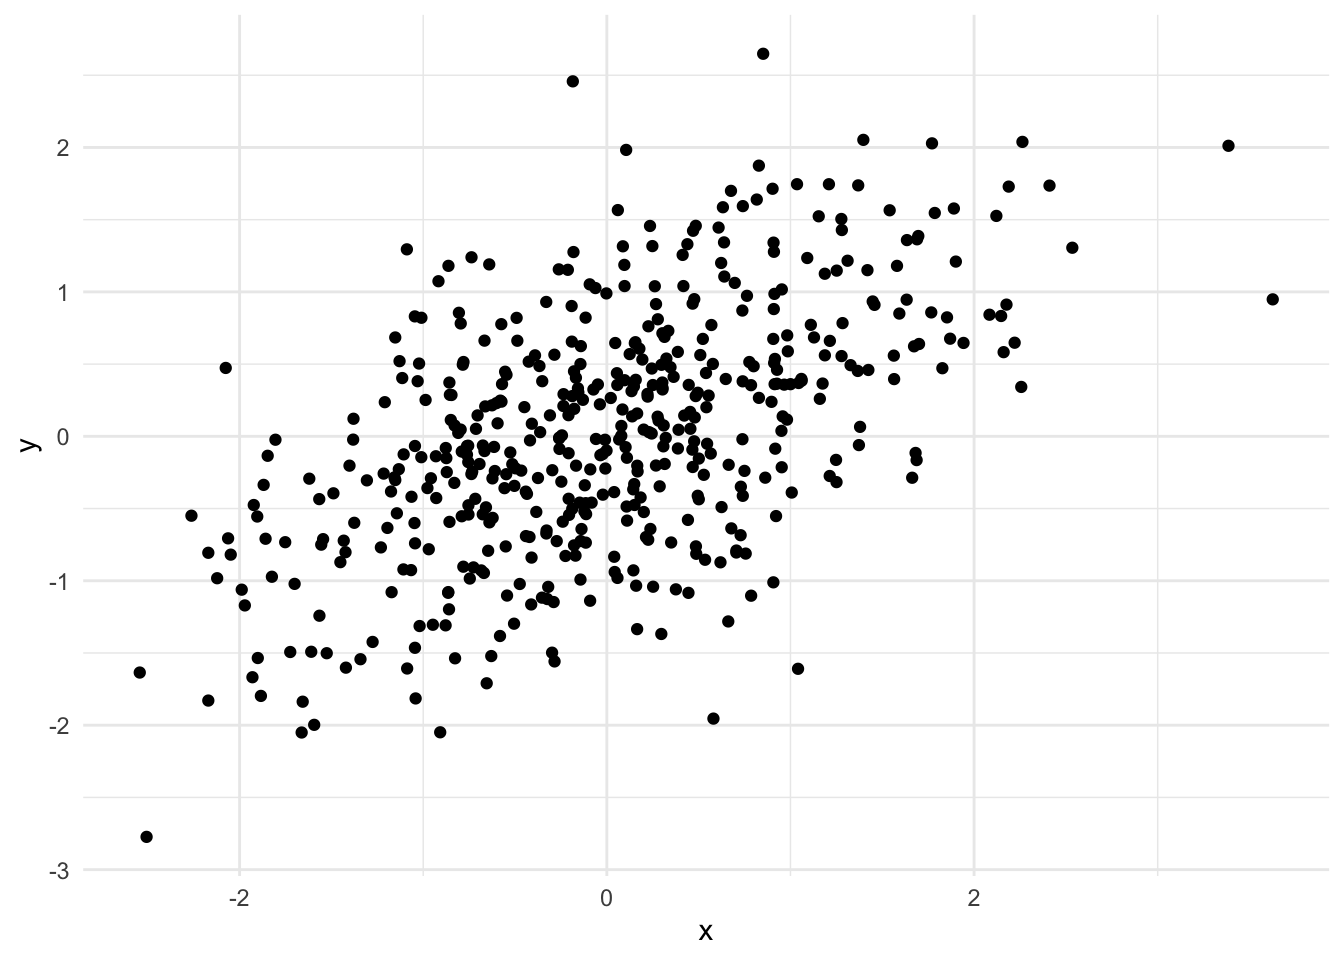
\includegraphics{introduction_files/figure-pdf/cor_viz-1.pdf}

}

\caption{Scatterplot of two variables.}

\end{figure}

Remember that correlation is testing for the presence of a linear
relationship, with -1 indicating a perfect negative relationship, 1
indicating a perfect positive relationship, and 0 indicating no
relationship. Before we see the actual correlation value for these two
variables, take a guess as to what value we are going to get!

Before we create our own function, we can use R's \texttt{cor} function
or numpy's \texttt{corrcoef} function. You should get something around
0.6.

\begin{Shaded}
\begin{Highlighting}[]
\CommentTok{\# Results for R and Python will be slightly}
\CommentTok{\# different due to different random number generators}
\FunctionTok{cor}\NormalTok{(x, y)}
\FunctionTok{np.corrcoef}\NormalTok{(x, y)}
\end{Highlighting}
\end{Shaded}

\begin{verbatim}
[1] 0.557
\end{verbatim}

When you guessed the value, were you close? If so, congrats! If not, try
fiddling with those knobs noted until things get a little clearer. But
now that we already know the answer, let's make sure that we can get the
same answer by working through the formula via code. The following takes
that initial formula approach and turns it into a function that we can
use to compute the correlation between any two variables. We'll then use
that function to compute the correlation between our \texttt{x} and
\texttt{y} variables.

\subsubsection{R}

\begin{Shaded}
\begin{Highlighting}[]
\NormalTok{my\_cor }\OtherTok{=} \ControlFlowTok{function}\NormalTok{(x, y) \{}
    \CommentTok{\# First, we need to compute the averages for x and y.}
    \CommentTok{\# The rest follows the formula.}
\NormalTok{    x\_bar }\OtherTok{=} \FunctionTok{mean}\NormalTok{(x)}
\NormalTok{    y\_bar }\OtherTok{=} \FunctionTok{mean}\NormalTok{(y)}

\NormalTok{    numerator }\OtherTok{=} \FunctionTok{sum}\NormalTok{((x }\SpecialCharTok{{-}}\NormalTok{ x\_bar) }\SpecialCharTok{*}\NormalTok{ (y }\SpecialCharTok{{-}}\NormalTok{ y\_bar))}

\NormalTok{    denominator }\OtherTok{=} \FunctionTok{sqrt}\NormalTok{(}
        \FunctionTok{sum}\NormalTok{((x }\SpecialCharTok{{-}}\NormalTok{ x\_bar)}\SpecialCharTok{\^{}}\DecValTok{2}\NormalTok{) }\SpecialCharTok{*} \FunctionTok{sum}\NormalTok{((y }\SpecialCharTok{{-}}\NormalTok{ y\_bar)}\SpecialCharTok{\^{}}\DecValTok{2}\NormalTok{)}
\NormalTok{    )}

\NormalTok{    numerator }\SpecialCharTok{/}\NormalTok{ denominator}
\NormalTok{\}}

\CommentTok{\# using the builtin functions}
\NormalTok{my\_cor2 }\OtherTok{=} \ControlFlowTok{function}\NormalTok{(x, y) \{}
    \FunctionTok{cov}\NormalTok{(x, y) }\SpecialCharTok{/}\NormalTok{ (}\FunctionTok{sd}\NormalTok{(x) }\SpecialCharTok{*} \FunctionTok{sd}\NormalTok{(y))}
\NormalTok{\}}

\FunctionTok{my\_cor}\NormalTok{(x, y)}
\end{Highlighting}
\end{Shaded}

\begin{verbatim}
[1] 0.557
\end{verbatim}

\subsubsection{Python}

\begin{Shaded}
\begin{Highlighting}[]
\KeywordTok{def}\NormalTok{ my\_cor(x, y):}
  \CommentTok{\# First, we need to compute the averages for x and y.}
  \CommentTok{\# The rest follows the formula.}
\NormalTok{    x\_bar }\OperatorTok{=}\NormalTok{ np.mean(x)}
\NormalTok{    y\_bar }\OperatorTok{=}\NormalTok{ np.mean(y)}
    
\NormalTok{    numerator }\OperatorTok{=}\NormalTok{ np.}\BuiltInTok{sum}\NormalTok{((x }\OperatorTok{{-}}\NormalTok{ x\_bar) }\OperatorTok{*}\NormalTok{ (y }\OperatorTok{{-}}\NormalTok{ y\_bar))}
    
\NormalTok{    denominator }\OperatorTok{=}\NormalTok{ np.sqrt(}
\NormalTok{      np.}\BuiltInTok{sum}\NormalTok{((x }\OperatorTok{{-}}\NormalTok{ x\_bar)}\OperatorTok{**}\DecValTok{2}\NormalTok{) }\OperatorTok{*}\NormalTok{ np.}\BuiltInTok{sum}\NormalTok{((y }\OperatorTok{{-}}\NormalTok{ y\_bar)}\OperatorTok{**}\DecValTok{2}\NormalTok{)}
\NormalTok{    )}

    \CommentTok{\# We will finish by dividing the numerator by the }
    \CommentTok{\# denominator.}
    \CommentTok{\# This will ensure that we have a value between {-}1 and 1.}
    \ControlFlowTok{return}\NormalTok{(numerator }\OperatorTok{/}\NormalTok{ denominator)}

\NormalTok{my\_cor(x, y)}
\end{Highlighting}
\end{Shaded}

\begin{verbatim}
0.5390318454354402
\end{verbatim}

It doesn't matter which language we use, the steps are largely the same
when we break it down into the individual pieces!

\subsection{Visualization}\label{visualization}

A long time ago, in a land far away, the authors of this book worked
together to help clients traverse the forests of data to reach their
modeling goals. While there were many great learning opportunities along
the way, working with clients showed us the kinds of help that people
really needed in adventuring with data and models. Even so, there were
many requests that made us grimace, and one stood atop Mount Ridiculous:
to produce a correlation matrix with 115 variables and export that
matrix to a spreadsheet. We still don't recommend such shenanigans, but
there are ways to try and understand correlation matrices. Since we were
in the business of helping people do their work better, one way we often
did so was via a \emph{corrplot}.

We'll start with a something manageable. We create a data set with six
variables of two sets: a, b , c, and x, y, z, and then we can take a
quick look at the correlation matrix.

\begin{longtable}{lrrrrrr}
\caption{Correlation matrix}\tabularnewline

\toprule
feature & a & b & c & x & y & z \\ 
\midrule
a & $1.00$ & $0.46$ & $0.45$ & $-0.16$ & $-0.21$ & $-0.19$ \\ 
b & $0.46$ & $1.00$ & $0.49$ & $-0.07$ & $-0.18$ & $-0.14$ \\ 
c & $0.45$ & $0.49$ & $1.00$ & $-0.16$ & $-0.23$ & $-0.20$ \\ 
x & $-0.16$ & $-0.07$ & $-0.16$ & $1.00$ & $0.49$ & $0.48$ \\ 
y & $-0.21$ & $-0.18$ & $-0.23$ & $0.49$ & $1.00$ & $0.52$ \\ 
z & $-0.19$ & $-0.14$ & $-0.20$ & $0.48$ & $0.52$ & $1.00$ \\ 
\bottomrule
\end{longtable}

Now we have the \emph{pairwise correlations} between all six of our
variables, with 1's on the diagonals (naturally, a variable has a
perfect correlation with itself). You can check out the lower diagonal
or the upper diagonal, because they contain the exact same information.
Quickly, though, find the interesting pattern in that matrix!

Producing the correlations between just 6 variables gives us 15
correlation coefficients to examine! You can see that you'll need to
spend more than a few seconds on finding the interesting patterns within
the data (or if there are any patterns at all). Our brains are oriented
towards vision, so we can use \emph{preattentive processing} elements,
like hue, saturation, and size, to make finding interesting patterns
easier.

Since we already have a correlation matrix, we can use various means to
find those patterns, which include visualizing the matrix itself,
network graphs and others. Here is one way to do it.

\begin{tcolorbox}[enhanced jigsaw, rightrule=.15mm, opacityback=0, left=2mm, bottomrule=.15mm, toprule=.15mm, arc=.35mm, colframe=quarto-callout-note-color-frame, leftrule=.75mm, breakable, colback=white]
\begin{minipage}[t]{5.5mm}
\textcolor{quarto-callout-note-color}{\faInfo}
\end{minipage}%
\begin{minipage}[t]{\textwidth - 5.5mm}

Some recommended R packages for visualizing a correlation matrix include
\texttt{corrr}, \texttt{ggcor}, and \texttt{corrplot}. For python, one
has options for \texttt{seaborn}, \texttt{pandas}, \texttt{biokit}, and
others.

\end{minipage}%
\end{tcolorbox}

\begin{figure}

{\centering 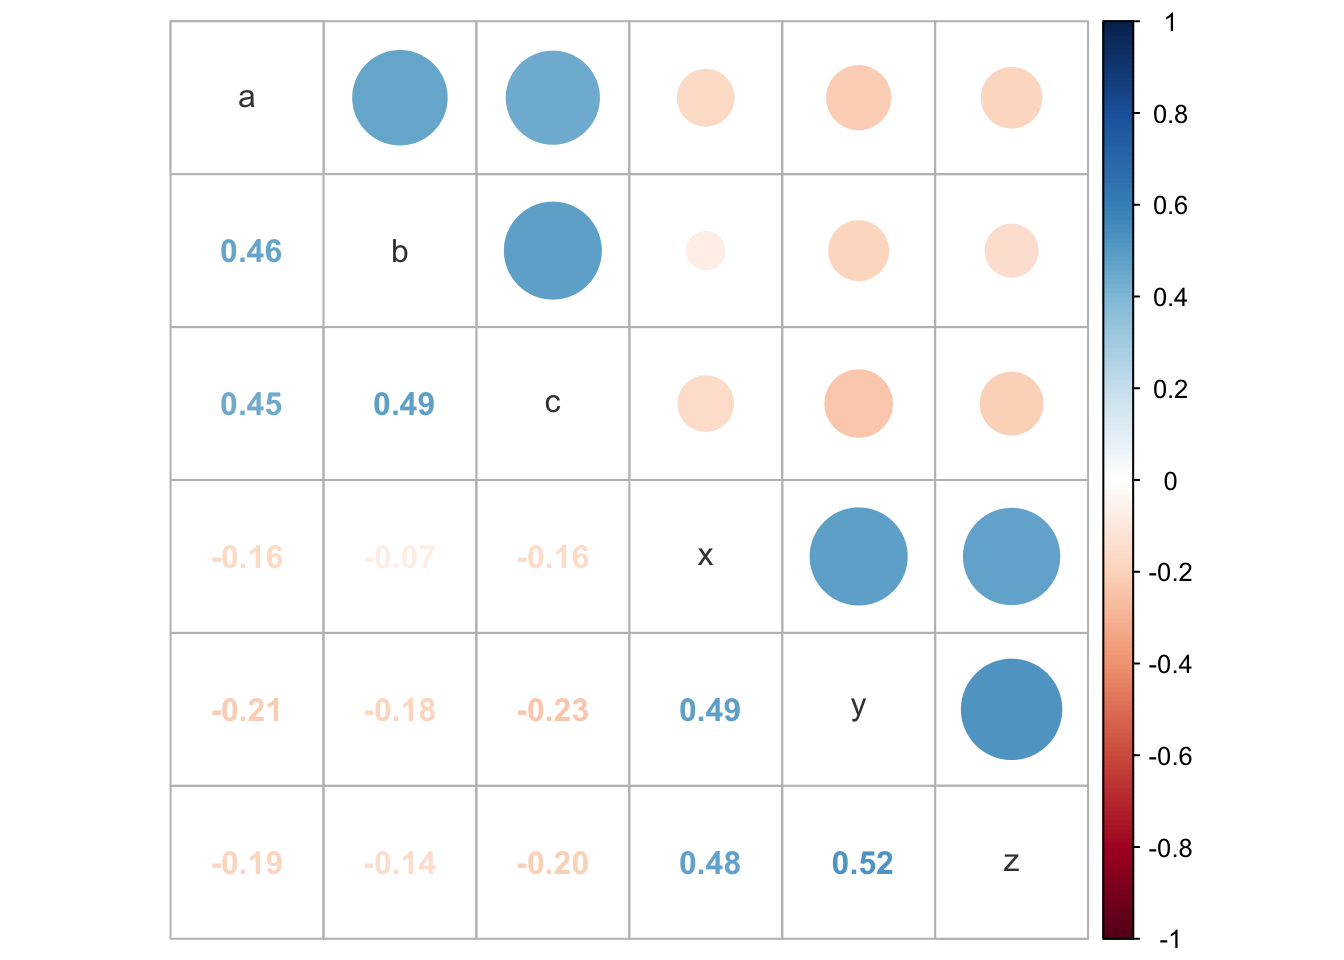
\includegraphics{introduction_files/figure-pdf/corrplot_demo-1.pdf}

}

\caption{Correlation matrix visualization}

\end{figure}

Let's break down what we're seeing just a little bit. The lower triangle
has the correlation values. It adds information, though, by changing the
hue by correlation value -- red for negative values and blue for
positive values -- and increasing the saturation as the correlation
value becomes stronger. The upper triangle contains the same
information, but the size of the circle is tied directly to the strength
of the correlation. You'll also notice that the weaker correlations are
more hidden in the visualization, allowing us to focus only on those
interesting relationships.

What do you think? Was it easier to spot the points of interest? It
looks like there is an a-b-c group and x-y-z group that are similarly
correlated within their respective groups. We can also see that the
a-b-c group is negatively correlated with the x-y-z group. Visualizing
the correlation matrix can usually make it easier to find those
interesting patterns.

\subsection{Commentary}\label{commentary}

The correlation is a starting point for understanding linear models,
which serve as the foundation for modeling in general. It is very
limited by only assessing linear relationships between variables, as
well as only pairwise relationships. Other metrics can overcome these,
but they have their own limitations. The basic Pearson-Product-Moment
correlation coefficient is still the most widely used and a typical
starting point in many data adventures.

Things to explore further next:

\begin{itemize}
\tightlist
\item
  Rank correlation (e.g., Spearman's rho, Kendall's tau)
\item
  Distance metrics (e.g., euclidean, manhattan, cosine)
\item
  Non-linear relationships and interactions (e.g., distance correlation,
  polynomial, splines)
\item
  Multivariate relationships (e.g., partial correlations, r-squared)
\end{itemize}

\section{Moving Towards An Excellent
Adventure}\label{moving-towards-an-excellent-adventure}

Remember the point we made about ``choosing your own adventure''?
Statistical modeling and programming is an adventure, even if you never
leave your desk! Every situation calls for choices to be made and every
choice you make will lead you down a different path. You will run into
errors, dead ends, and you might even find that you've spent
considerable time to conclude that nothing interesting is happening in
your data. This, no doubt, is part of the fun and all of those struggles
make success that much sweeter. Like every adventure, things might not
be immediately clear and you might find yourself in perilous situations!
If you find that something isn't making sense upon your first read, that
is okay. Both authors have spent considerable time mulling over models
and foggy ideas during our assorted (mis)adventures; nobody should
expect to master complex concepts on a single read through! In any arena
where you strive to develop skills, distributed practice and repetition
are essential. When concepts get tough, step away from the book, and
come back with a fresh mind.

Thanks for coming on this adventure with us and welcome to our
\emph{Book of Models}.

This is a test reference (\textbf{hastie\_elements\_2009?}).

\part{Linear Models}

\chapter{The Foundation}\label{the-foundation}

\begin{quote}
It is the chief characteristic of data science that it works. ― Isaac
Asimov (paraphrased)
\end{quote}

Packages needed or useful for this chapter include:

\subsubsection{R}

\begin{Shaded}
\begin{Highlighting}[]
\FunctionTok{library}\NormalTok{(tidyverse)}
\end{Highlighting}
\end{Shaded}

\subsubsection{Python}

\begin{Shaded}
\begin{Highlighting}[]
\ImportTok{import}\NormalTok{ numpy }\ImportTok{as}\NormalTok{ np}
\ImportTok{import}\NormalTok{ pandas }\ImportTok{as}\NormalTok{ pd}
\ImportTok{import}\NormalTok{ statsmodels.formula.api }\ImportTok{as}\NormalTok{ smf}
\end{Highlighting}
\end{Shaded}

\section{Introducing the Greatest Of All
Time}\label{introducing-the-greatest-of-all-time}

Now that you have some idea of what you're getting into, it's time to
dive in! We'll start things off by covering the building block of all
modeling, and a solid understanding here will provide you the basis for
just about anything that comes after, no matter how complex it gets. The
\textbf{linear model} is our starting point. At first glance, it may
seem like a very simple model, but it's actually quite powerful and
flexible, able to take in different types of inputs, handle nonlinear
relationships, temporal and spatial relations, clustering, and more.
Linear models have a long history, with even the formal and scientific
idea behind correlation and linear regression being well over a century
old\footnote{Peirce \& Bowditch were well ahead of Pearson and Galton
  (\textbf{rovine2004peirce?}).}! And in that time, the linear model is
far and away the most used model out there. But before we start talking
about the \emph{linear} model, we need to talk about what a
\textbf{model} is in general.

\subsection{What is a Model?}\label{what-is-a-model}

At its core, a model is just an \textbf{idea}. It's a way of thinking
about the world, about how things work, how things change over time, how
things are different from each other, and how they are similar. The
underlying thread is that \textbf{a model expresses relationships} about
things in the world around us. One can also think of a \textbf{model as
a tool}, one that allows us to take information, in the form of data,
and act on it in some way. Just like other ideas (and tools), models
have consequences in the real world, and they can be used wisely or
foolishly.

On a practical level, a model is expressed through a particular
language, math, but don't let that worry you if you're not so inclined.
As it's still just an idea at its core, the idea is the most important
thing to understand about a model. The \textbf{math is just a formal way
of expressing the idea} in a manner that can be communicated and
understood by others in a standard way, and math can help make the idea
precise. But in everyday terms, we're trying to understand things like
how the amount of sleep relates to cognitive functioning, how the
weather affects the number of people who visit a park, how much money to
spend on advertising to increase sales, how to detect fraud, and so on.
Any of these could form the basis of a model, as they stem from
scientifically testable ideas, and they all express relationships
between things we are interested in, possibly even with an implication
of causal relations.

If you wanted to run a linear model to understand the relationship
between sleep and cognitive functioning, you might express it in code
as:

\subsubsection{R}

\begin{Shaded}
\begin{Highlighting}[]
\FunctionTok{lm}\NormalTok{(cognitive\_functioning }\SpecialCharTok{\textasciitilde{}}\NormalTok{ sleep)}
\end{Highlighting}
\end{Shaded}

\subsubsection{Python}

\begin{Shaded}
\begin{Highlighting}[]
\ImportTok{from}\NormalTok{ statsmodels.formula.api }\ImportTok{import}\NormalTok{ ols}

\NormalTok{model }\OperatorTok{=}\NormalTok{ ols(}\StringTok{\textquotesingle{}cognitive\_functioning \textasciitilde{} sleep\textquotesingle{}}\NormalTok{, data}\OperatorTok{=}\NormalTok{df).fit()}
\end{Highlighting}
\end{Shaded}

Very easy! But that's all it takes to express a straightforward idea. In
this case, we're saying that cognitive functioning is a linear
(function) of sleep. By the end of this chapter you'll also know why R's
function is \texttt{lm} (linear model) and the {statsmodels} function is
\texttt{ols}, but both are doing the same thing.

\section{Key ideas}\label{key-ideas-1}

We can pose a few concepts key to understanding models. This is not an
exhaustive list, but it's a good start. We'll cover each of these as we
go along.

\begin{itemize}
\tightlist
\item
  What a model is: The model as an idea
\item
  Features, targets, and input-output mappings: how do we get from input
  to output?
\item
  Prediction: how do we use a model?
\item
  Interpretation: what does a model tell us?

  \begin{itemize}
  \tightlist
  \item
    Prediction underlies all interpretation
  \item
    We can interpret a model at the feature level and as a whole
  \end{itemize}
\end{itemize}

As we go along and cover these concepts, be sure that you feel you have
the `gist' of what we're talking about. Almost everything of what comes
after linear models builds on these ideas, so it's important to have a
firm grasp before climbing to new heights.

Chapter goals:

\begin{itemize}
\tightlist
\item
  Understand what a model is conceptually
\item
  Understand what a linear model is and how features are mapped to the
  target
\item
  Be able to get predictions from our model
\item
  Be able to understand the results of a model at a basic level
\item
  Get a sense of complexity and other issues
\end{itemize}

\section{What goes into a model?}\label{what-goes-into-a-model}

\subsection{Features and Targets}\label{features-and-targets}

In the context of a model, how we specify the nature of the relationship
depends on the context. In the interest of generality, we'll refer to
the \textbf{target} as what we want to explain, and \textbf{features} as
those aspects of the data we will use to explain it. Because people come
at data from a variety of contexts, they often use different terminology
to mean the same thing. The table below shows some of the common terms
used to refer to features and targets.

\hypertarget{tbl-feature-target-names}{}
\begin{longtable}{ll}
\caption{\label{tbl-feature-target-names}Common Terms for Features and Targets }\tabularnewline

\toprule
Feature & Target \\ 
\midrule\addlinespace[2.5pt]
independent variable & dependent variable \\ 
predictor variable & response \\ 
explanatory variable & outcome \\ 
covariate & label \\ 
x & y \\ 
input & output \\ 
right-hand side & left-hand side \\ 
\bottomrule
\end{longtable}

Some of these actually suggest a particular type of relationship (e.g.,
a causal relationship, an experimental setting), but we'll typically
avoid those terms if we can. In the end, we may use many of these words
to describe things so that you are comfortable with the terminology, but
typically we'll stick with \textbf{features} and \textbf{targets} for
the most part. In our opinion, this terminology has the least hidden
assumptions/implications.

\subsection{Expressing Relationships}\label{expressing-relationships}

As noted, a model is a way of expressing a relationship between a set of
features and a target, and one way of thinking about this is in terms of
\textbf{inputs} and \textbf{outputs}. But how can we go from input to
output? Well to begin, we assume that the features and target are
\textbf{correlated}, i.e.~that there is some relationship between the x
and y. If so, then we can ultimately use the features to
\textbf{predict} the target. In the simplest setting a correlation
implies a relationship where x and y typically move up and down together
(left plot) or they move in opposite directions where x goes up and y
goes down (right plot).

\begin{figure}

{\centering 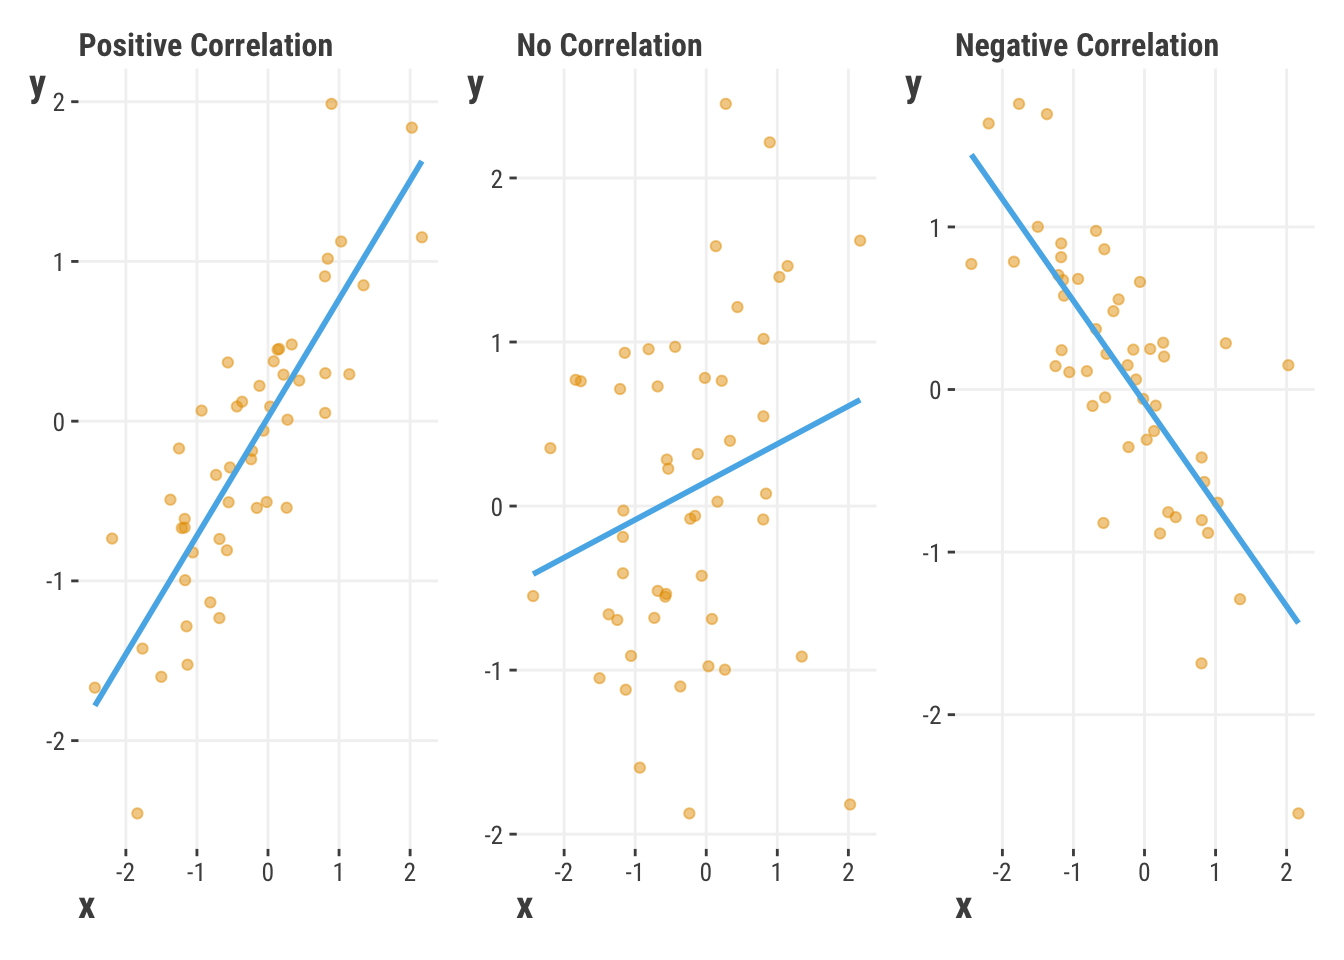
\includegraphics{linear_models_files/figure-pdf/fig-corr-plot-1.pdf}

}

\caption{\label{fig-corr-plot}Correlation}

\end{figure}

In addition, the typical correlation suggests a linear relationship.
There are many types of correlation metrics, but the most common one,
the \textbf{Pearson correlation}, is explicitly a measure of the linear
relationship between two variables. It's expressed as a number between
-1 and 1, where 0 means there is no linear relationship. As we move
closer to a 1.0 correlation value, we would see a tighter scatterplot
like the one on the left, until it became a straight line. The same
happens for the negative relationship as we get closer to a value of -1.
If we have only one feature and target, the Pearson correlation reflects
the exact result of the linear model we'd conduct. But even with
multiple features, we often use a version of the Pearson R to help us
understand how the features account for the target's variability.

\section{\texorpdfstring{\emph{THE} Linear
Model}{THE Linear Model}}\label{the-linear-model}

The linear model is perhaps the simplest \emph{functional} model we can
use to express a relationship between features and targets. And because
of that, it's possibly still the most common model used in practice, and
it is the basis for many types of other models. Why don't we run one
now?

The following dataset has individual \hyperref[app-data-review]{movie
reviews} and contains the rating (1-5 stars scale), along with features
pertaining to the review (e.g., word count, etc.), those that regard the
reviewer (e.g., age) and features about the movie (e.g., genre, release
year). We'll use the linear model to predict the rating from the length
of the review in terms of word count.

For our first linear model, we'll keep things simple. Let's predict the
rating from the length of the review in terms of word count. We'll use
the \texttt{lm()} function in R and the \texttt{ols()} function in
Python\footnote{We actually are using the \texttt{smf.ols} approach
  because it is modeled on the R approach.} to fit the model. Both
functions take a formula as the first argument, which is a way of
expressing the relationship between the features and target. The formula
is expressed as \texttt{y\ \textasciitilde{}\ x1\ +\ x2\ +\ ...}, where
\texttt{y} is the target name and \texttt{x} are the feature names. We
also need to specify what the data object is, typically a data frame.

\subsubsection{R}

\begin{Shaded}
\begin{Highlighting}[]
\NormalTok{df\_reviews }\OtherTok{=} \FunctionTok{read\_csv}\NormalTok{(}\StringTok{"data/movie\_reviews.csv"}\NormalTok{)}

\NormalTok{model\_reviews }\OtherTok{=} \FunctionTok{lm}\NormalTok{(rating }\SpecialCharTok{\textasciitilde{}}\NormalTok{ word\_count, }\AttributeTok{data =}\NormalTok{ df\_reviews)}

\FunctionTok{summary}\NormalTok{(model\_reviews)}
\end{Highlighting}
\end{Shaded}

\begin{verbatim}

Call:
lm(formula = rating ~ word_count, data = df_reviews)

Residuals:
    Min      1Q  Median      3Q     Max 
-2.0648 -0.3502  0.0206  0.3352  1.8498 

Coefficients:
            Estimate Std. Error t value Pr(>|t|)    
(Intercept)  3.49164    0.04236    82.4   <2e-16 ***
word_count  -0.04268    0.00369   -11.6   <2e-16 ***
---
Signif. codes:  0 '***' 0.001 '**' 0.01 '*' 0.05 '.' 0.1 ' ' 1

Residual standard error: 0.591 on 998 degrees of freedom
Multiple R-squared:  0.118, Adjusted R-squared:  0.118 
F-statistic:  134 on 1 and 998 DF,  p-value: <2e-16
\end{verbatim}

\subsubsection{Python}

\begin{Shaded}
\begin{Highlighting}[]
\NormalTok{df\_reviews }\OperatorTok{=}\NormalTok{ pd.read\_csv(}\StringTok{\textquotesingle{}data/movie\_reviews.csv\textquotesingle{}}\NormalTok{)}

\NormalTok{model\_reviews }\OperatorTok{=}\NormalTok{ smf.ols(}\StringTok{\textquotesingle{}rating \textasciitilde{} word\_count\textquotesingle{}}\NormalTok{, data }\OperatorTok{=}\NormalTok{ df\_reviews).fit()}

\NormalTok{model\_reviews.summary(slim }\OperatorTok{=} \VariableTok{True}\NormalTok{)}
\end{Highlighting}
\end{Shaded}

\begin{verbatim}
<class 'statsmodels.iolib.summary.Summary'>
"""
                            OLS Regression Results                            
==============================================================================
Dep. Variable:                 rating   R-squared:                       0.118
Model:                            OLS   Adj. R-squared:                  0.118
No. Observations:                1000   F-statistic:                     134.1
Covariance Type:            nonrobust   Prob (F-statistic):           3.47e-29
==============================================================================
                 coef    std err          t      P>|t|      [0.025      0.975]
------------------------------------------------------------------------------
Intercept      3.4916      0.042     82.431      0.000       3.409       3.575
word_count    -0.0427      0.004    -11.580      0.000      -0.050      -0.035
==============================================================================

Notes:
[1] Standard Errors assume that the covariance matrix of the errors is correctly specified.
"""
\end{verbatim}

For such a simple model, we certainly have a lot to unpack here! Don't
worry, you'll eventually come to know what it all means. But it's nice
to know how easy it is to get the results!

We'll start with the fact that the linear model posits a \textbf{linear
combination} of the features. A linear combination is just a sum of the
features, each of which has been multiplied by some specific value. That
value is often called a \textbf{coefficient}, or possibly
\textbf{weight}, depending on the context. The linear model is expressed
as (math incoming!):

\begin{equation}\protect\hypertarget{eq-lm-basic}{}{
y = b_0 + b_1x_1 + b_2x_2 + ... + b_nx_n
}\label{eq-lm-basic}\end{equation}

\begin{itemize}
\tightlist
\item
  \(y\) is the target.
\item
  \(x_1, x_2, ... x_n\) are the features.
\item
  \(b_0\) is the intercept, which is kind of like a baseline value or
  offset. If we had no features at all it would just be the mean of the
  target.
\item
  \(b_1, b_2, ... b_n\) are the coefficients or weights for each
  feature.
\end{itemize}

But lets start with something simpler, let's say you want to take a sum
of several features. In math you would write it as:

\[
x_1 + x_2 + ... + x_n
\]

In the previous equation, x is the feature and n is the number
identifier for the features, so \(x_1\) is the first feature, \(x_2\)
the second, and so on. \(x\) is an arbitrary designation, you could use
any letter, symbol you want, or even better, would be the actual feature
name. Now look at the linear model.

\[
y = x_1 + x_2 + ... + x_n
\]

In this case, the function is \emph{just a sum}, something so simple we
do it all the time. In the linear model sense though, we're actually
saying a bit more. Another way to understand that equation is that
\emph{y is a function of x}. We don't show any coefficients, i.e.~the bs
in our initial depiction, but technically it's as if each coefficient
was a value of 1. In other words, for this simple linear model, we're
saying that each feature contributes in an identical fashion to the
target.

In practice, features will not contribute in the same ways, because they
correlate with the target differently or are on different scales. So if
we want to relate some feature, x1, and some other feature, x2, to
target y, we probably would not assume that they both contribute in the
same way from the beginning. We might give relatively more weight to x1
than x2. In the linear model, we express this by multiplying each
feature by a different coefficient. So the linear model is really just a
sum of the features multiplied by their coefficients, i.e.~a
\emph{weighted sum}. In fact, we're saying that each feature contributes
to the target in proportion to the coefficient. So if we have a feature
x1 and a coefficient b1, then the contribution of x1 to the target is
b1*x1. If we have a feature x2 and a coefficient b2, then the
contribution of x2 to the target is b2*x2. And so on. So the linear
model is really just a sum of the features multiplied by their
coefficients.

For our model, here is the mathematical representation:

\[
\textrm{rating} = b_0 + b_1 \cdot \textrm{word\_count}
\]

And with the actual results of our model:

\[
\textrm{rating} = 3.49 + -0.04 \cdot \textrm{word\_count}
\]

Not too complicated we hope! But let's make sure we see what's going on
here just a little bit more.

\begin{itemize}
\tightlist
\item
  Our \emph{idea} is that the length of the review is in some way
  related to the eventual rating given to the movie.
\item
  Our \emph{target} is rating, and the \emph{feature} is the word count
\item
  We \emph{map the feature to the target} via the linear model, which
  provides an initial understanding of how the feature is related to the
  target. In this case, we start with a baseline of 3.49. This value
  makes sense only in the case of a rating with no review, but we have
  reviews for every observation, so it's not very meaningful as is.
  We'll talk about ways to get a more meaningful intercept later, but
  for now, that is our starting point. Moving on, if we add a single
  word to the review, we expect the rating to go down by -0.04 stars. So
  if we had a review that was 10 words long, i.e., the mean word count,
  we would predict a rating of 3.49 + 10*-0.04 = 3.1 stars.
\end{itemize}

\subsection{Models as a Graph}\label{models-as-a-graph}

We can also express the linear model as a graph, which can be a very
useful way to think about models in a visual fashion, and as we see
others, can help us literally see how different models relate to one
another. In the following, we have three features predicting a single
target, so we have three nodes for the features, and a single node for
the target. The feature nodes are connected to the target node by an
edge, which is labeled with the coefficient. The graph below shows a
basic linear model.

\hypertarget{graph-lm}{}
\begin{figure}[H]

{\centering \includegraphics[width=4in,height=3.5in]{linear_models_files/figure-latex/dot-figure-1.png}

}

\end{figure}

Linear Model as a Graph

So at this point you have the basics of what a linear model is and how
it works. But there is a lot more to it than that. Just getting the
model is easy enough, but we need to be able to use it and understand
the details better, so we'll get into that now!

\section{What do we do with a model?}\label{what-do-we-do-with-a-model}

Once we have a working model, there are two primary ways we can use it.
One way to use a model is to help us understand the relationships
between the features and our outcome of interest. In this way the focus
can be said to be on \textbf{explanation}, or interpreting the model
results. The other way to use a model is to use it to make estimates
about the outcome for specific observations, often ones we haven't seen
in our data. In this way the focus is on \textbf{prediction}. In
practice, we often do both, but the focus is usually on one or the
other. We'll cover both in detail here, starting with prediction.

\subsection{Prediction}\label{prediction}

It may not seem like much at first, but a model is of no use if it can't
be used to make predictions about what we can expect in the world around
us. Once our model has been \emph{fit} to the data, we can obtain our
predictions by plugging in values for the features that we are
interested in, and, using the corresponding weights and other parameters
that have been estimated, come to a guess about a specific observation.
Let's go back to our results, starting with a simpler depiction.

\begin{longtable*}{lrrrrrr}
\toprule
feature & estimate & std\_error & statistic & p\_value & conf\_low & conf\_high \\ 
\midrule\addlinespace[2.5pt]
intercept & \textcolor[HTML]{404040}{$3.49$} & \textcolor[HTML]{404040}{$0.04$} & \textcolor[HTML]{404040}{$82.43$} & \textcolor[HTML]{404040}{$0.00$} & \textcolor[HTML]{404040}{$3.41$} & \textcolor[HTML]{404040}{$3.57$} \\ 
word\_count & \textcolor[HTML]{404040}{$-0.04$} & \textcolor[HTML]{404040}{$0.00$} & \textcolor[HTML]{404040}{$-11.58$} & \textcolor[HTML]{404040}{$0.00$} & \textcolor[HTML]{404040}{$-0.05$} & \textcolor[HTML]{404040}{$-0.04$} \\ 
\bottomrule
\end{longtable*}

The table shows the \textbf{coefficient} for each feature including the
intercept, which is our starting point. In this case, the coefficient
for word count is -0.04, which means that for every additional word in
the review, the rating goes down by -0.04 stars. So if we had a review
that was 10 words long, we would \emph{predict} a rating of 3.49 +
10*-0.04 = 3.1 stars.

When we're talking about predictions for a linear model, we usually will
see this as the following mathematically:

\[
\hat{y} = b_0 + b_1x_1 + b_2x_2 + ... + b_nx_n
\]

What is \(\hat{y}\)? The hat over the \(y\) just means that it's a
predicted value of the model, rather than the one we actually observe.
In fact, we were missing something in our previous depictions of the
linear model. We need to add what is usually referred to as an
\textbf{error term}, \(\epsilon\), to account for the fact that our
predictions will not be perfect\footnote{In most circumstances, if you
  ever have perfect prediction, or even near perfect prediction, the
  usual issues are that you have either asked a rather obvious/easy
  question of your data (e.g., predicting whether an image is of a human
  or a car), or have accidentally included the target in your features
  (or a combination of them) in some way.}. So the full linear model is:

\[
y = b_0 + b_1x_1 + b_2x_2 + ... + b_nx_n + \epsilon
\]

The error term is a random variable that represents the difference
between the actual value and the predicted value. We can't know what the
error term is, but we can estimate it. We'll talk more about that in the
section on {[}estimation{]}{[}\#estimation{]}.

\subsection{What kinds of predictions can we
get?}\label{what-kinds-of-predictions-can-we-get}

What predictions we get depends on the type of model we are using. For
the linear model, we can get predictions for the target, which is a
\textbf{continuous variable}. Very commonly, we also can get predictions
for a \textbf{categorical target}, such as whether the rating is `good'
or `bad'. This simple breakdown pretty much covers everything, as we
typically would be predicting a continuous variable or a categorical
variable, or more of them, like multiple continuous variables, or a
target with multiple categories, or sequences of categories
(e.g.~words). In our case, we can get predictions for the rating, which
is a number between 1 and 5. Had our target been a binary good vs.~bad
rating, our predictions would still be numeric, and usually expressed as
a probability between 0 and 1. We then would convert that probability to
a class of good or bad depending on a chosen probability cutoff. We'll
talk about how to get predictions for categorical targets later.

We saw a prediction for a single observation, but we can also get
predictions for multiple observations at once. In fact, we can get
predictions for all observations in our dataset. Besides that, we can
also get predictions for observations that we don't have data for. The
following shows how we can get predictions for all data, and for a
single observation with a word count of 5.

\subsubsection{R}

\begin{Shaded}
\begin{Highlighting}[]
\NormalTok{all\_predictions }\OtherTok{=} \FunctionTok{predict}\NormalTok{(model\_reviews)}
\NormalTok{single\_prediction }\OtherTok{=} \FunctionTok{predict}\NormalTok{(model\_reviews, }\AttributeTok{newdata =} \FunctionTok{data.frame}\NormalTok{(}\AttributeTok{word\_count =} \DecValTok{5}\NormalTok{))}
\end{Highlighting}
\end{Shaded}

\subsubsection{Python}

\begin{Shaded}
\begin{Highlighting}[]
\NormalTok{all\_predictions   }\OperatorTok{=}\NormalTok{ model\_reviews.predict()}
\NormalTok{single\_prediction }\OperatorTok{=}\NormalTok{ model\_reviews.predict(pd.DataFrame(\{}\StringTok{\textquotesingle{}word\_count\textquotesingle{}}\NormalTok{: [}\DecValTok{5}\NormalTok{]\}))}
\end{Highlighting}
\end{Shaded}

Here is a plot of our predictions versus the actual ratings\footnote{Word
  count is \textbf{discrete}- it can only take whole numbers like 3 or
  20, and it is our only feature. Because of this, we can only make very
  limited predicted rating values, while the observed rating can take on
  many other values. Because of this, the true plot would show a more
  banded result with many points overlapping, so we use a technique
  called \textbf{jittering} to move the points around a little bit so we
  can see them all. The points are still roughly in the same place, but
  they are moved around a little bit so we can see them all.}. The
reference line is where the points would fall if we had perfect
prediction. We can see that the predictions are definitely not perfect,
but they are not completely off base either. We'll talk about how to
assess the quality of our predictions later, but we can at least get a
sense that we have a correspondence relationship between our predictions
and target, which is definitely better than not having a relationship at
all!

!{[}Predictions vs.~Actual
Ratings{]}(linear\_models\_files/figure-pdf/my-first-model-predictions-plot-1.pdf)

Now let's look at what our prediction looks like for a single
observation, and we'll add in a few more- one for 10 words, and one for
a 50 word review, which is beyond the length of any review in this
dataset, and one for 12.3 words, which isn't even possible for this
data.

\hypertarget{tbl-predictions}{}
\begin{longtable}{rr}
\caption{\label{tbl-predictions}Predictions for Specific Observations }\tabularnewline

\toprule
Word Count & Predicted Rating \\ 
\midrule\addlinespace[2.5pt]
\textcolor[HTML]{404040}{$5.0$} & \textcolor[HTML]{404040}{$3.3$} \\ 
\textcolor[HTML]{404040}{$10.0$} & \textcolor[HTML]{404040}{$3.1$} \\ 
\textcolor[HTML]{404040}{$12.3$} & \textcolor[HTML]{404040}{$3.0$} \\ 
\textcolor[HTML]{404040}{$50.0$} & \textcolor[HTML]{404040}{$1.4$} \\ 
\bottomrule
\end{longtable}

The values reflect the negative coefficient from our model, reflecting a
decreasing relationship. Further more, we see the power of the model's
ability to make predictions for what we can't see. Maybe we limited our
data review size, but we know there are 50 word reviews out there, and
we can still make a guess as to what the rating would be for such a
review. Maybe in another case, we know a group of people who have on
average 12.3 word reviews, and we can make a guess as to what the
average rating would be for that group. Our model doesn't know anything
about the context of the data, but we can use our knowledge to make
predictions about the world around us. This is a very powerful
capability, and it's one of the main reasons we use models in the first
place.

\subsection{Prediction Error}\label{prediction-error}

As we have seen, predictions are not perfect, and an essential part of
the modeling endeavor is to better understand these errors and why they
occur. In addition, error assessment is the fundamental way in which we
assess a model's performance, and, by extension, compare that
performance to other models. In general, prediction error is the
difference between the actual value and the predicted value or some
function of it, and in statistical models, is also often called the
\textbf{residual}. We can look at these individually, or we can look at
them in aggregate with a single metric.

Let's start with looking at the residuals visually. Often the modeling
package you use will have this as a default plotting method when doing a
standard linear regression, so it's wise to take advantage of it. We
plot both the distribution of raw error scores and the cumulative
distribution of absolute prediction error. Here we see a couple things.
First, the distribution is roughly normal, which is a good thing, since
statistical linear regression assumes our prediction error is normally
distributed. Second, we see that the mean of the errors is zero, which
is a consequence of linear regression, and the reason we look at the
mean squared error rather than the mean error when assessing model
performance. We can also see that most of our predictions are within 1
star rating.

\begin{figure}

{\centering 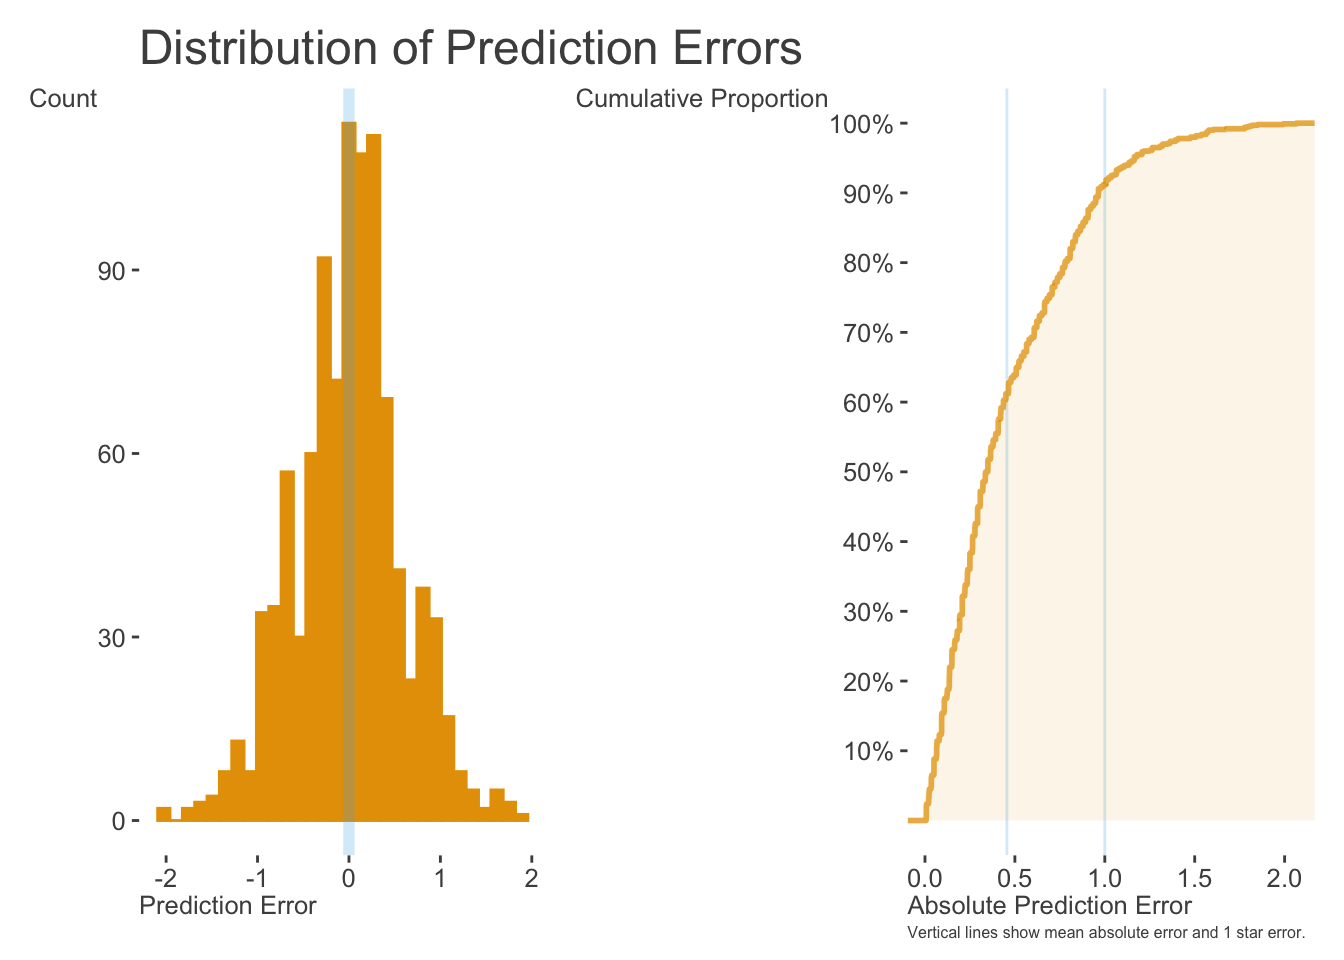
\includegraphics{linear_models_files/figure-pdf/my-first-model-error-plot-1.pdf}

}

\caption{Distribution of Prediction Errors}

\end{figure}

Of more practical concern however, is that we don't see extreme values
or clustering that might indicate a failure on the part of the model to
pick up certain segments of the data. It still is good to look at the
extremes just in case we can pick up on some aspect of the data that we
could potentially incorporate into the model.

Looking at our worst prediction in absolute terms, we see the
observation has a typical word count, and so our simple model will just
predict a fairly typical rating. But the actual rating is 1, which is
2.1 away from our prediction, a very noticeable difference.

\hypertarget{tbl-worst-prediction}{}
\begin{longtable}{rrr}
\caption{\label{tbl-worst-prediction}Worst Prediction }\tabularnewline

\toprule
rating & prediction & word\_count \\ 
\midrule\addlinespace[2.5pt]
\textcolor[HTML]{404040}{$1.0$} & \textcolor[HTML]{404040}{$3.1$} & \textcolor[HTML]{404040}{$10$} \\ 
\bottomrule
\end{longtable}

We can also get an overall assessment of the prediction error. In the
case of the linear model we've been looking at, we can express this in a
single metric as the sum or mean of our (squared) errors, the latter of
which is a very commonly used modeling metric- \textbf{MSE} or
\textbf{mean squared error}, or also, its square root - \textbf{RMSE} or
\textbf{root mean squared error}.

If we look back at our results, we can see this expressed as the part of
the output or as an attribute of the model\footnote{The actual divisor
  for linear regression output depends on the complexity of the model,
  and in this case the sum of the squared errors is divided by N-2 (due
  to estimating the intercept and coefficient) instead of N. This is a
  technical detail that would only matter for data too small to make
  much of in the first place, and not important for our purposes here.}.
The RMSE is more interpretable, and it gives us a sense that we can
expect an average prediction error for rating of 0.59. Given that the
rating is on a 1-5 scale, this maybe isn't bad, but we could definitely
hope to do better than get within roughly half a point on this scale.
We'll talk about ways to improve this later.

\subsubsection{R}

\begin{Shaded}
\begin{Highlighting}[]
\FunctionTok{summary}\NormalTok{(model\_reviews) }\CommentTok{\# \textquotesingle{}Residual standard error\textquotesingle{} is approx RMSE}
\end{Highlighting}
\end{Shaded}

\begin{verbatim}

Call:
lm(formula = rating ~ word_count, data = df_reviews)

Residuals:
    Min      1Q  Median      3Q     Max 
-2.0648 -0.3502  0.0206  0.3352  1.8498 

Coefficients:
            Estimate Std. Error t value Pr(>|t|)    
(Intercept)  3.49164    0.04236    82.4   <2e-16 ***
word_count  -0.04268    0.00369   -11.6   <2e-16 ***
---
Signif. codes:  0 '***' 0.001 '**' 0.01 '*' 0.05 '.' 0.1 ' ' 1

Residual standard error: 0.591 on 998 degrees of freedom
Multiple R-squared:  0.118, Adjusted R-squared:  0.118 
F-statistic:  134 on 1 and 998 DF,  p-value: <2e-16
\end{verbatim}

\subsubsection{Python}

\begin{Shaded}
\begin{Highlighting}[]
\NormalTok{np.sqrt(model\_reviews.scale)   }\CommentTok{\# RMSE}
\end{Highlighting}
\end{Shaded}

\begin{verbatim}
0.590728780660127
\end{verbatim}

At this point you have the gist of prediction and prediction error, but
there is a lot more to it. More detail can be found in the
\hyperref[estimation]{estimation chapter}, since we often estimate the
parameters of our model by picking those that will reduce the prediction
error the most. For now, let's move on to the other main use of models,
which is to help us understand the relationships between the features
and the target, or \textbf{explanation}.

\section{How do we interpret the
model?}\label{how-do-we-interpret-the-model}

When it comes to interpreting the results of our model, there are a lot
of tools at our disposal, though many of the tools we can ultimately use
depend on the specifics of the model we have employed. In general
though, we can group our understanding approach to that of the
\textbf{feature level} and the \textbf{model level}. A feature level
understanding regards the relationship between a single feature and the
target. Beyond that, we also attempt comparisons of feature
contributions to prediction, i.e.~relative importance. Model level
interpretation is focused on assessments of how well the model `fits'
the data, or more generally, predictive performance. We'll start with
the feature level, and then move on to the model level.

\subsection{Feature Level}\label{feature-level}

As mentioned, at the feature level, we are primarily concerned with the
relationship between a single feature and the target. More specifically,
we are interested in the direction and magnitude of the relationship,
but in general, it all boils down to how a feature induces change in the
target. For numeric features, we are curious about the change in the
target given some amount of change in the feature. For categorical
features it's the same, but often we like to express the change in terms
of group mean differences or something similar, since the order of
categories is not usually meaningful. Key to the feature level
interpretation is the specific predictions made at key feature values.

\subsubsection{Basics}\label{basics}

Let's start with the basics by looking again at our coefficient table
from the model output.

\begin{longtable*}{lrrrrrr}
\toprule
feature & estimate & std\_error & statistic & p\_value & conf\_low & conf\_high \\ 
\midrule\addlinespace[2.5pt]
intercept & \textcolor[HTML]{404040}{$3.49$} & \textcolor[HTML]{404040}{$0.04$} & \textcolor[HTML]{404040}{$82.43$} & \textcolor[HTML]{404040}{$0.00$} & \textcolor[HTML]{404040}{$3.41$} & \textcolor[HTML]{404040}{$3.57$} \\ 
word\_count & \textcolor[HTML]{404040}{$-0.04$} & \textcolor[HTML]{404040}{$0.00$} & \textcolor[HTML]{404040}{$-11.58$} & \textcolor[HTML]{404040}{$0.00$} & \textcolor[HTML]{404040}{$-0.05$} & \textcolor[HTML]{404040}{$-0.04$} \\ 
\bottomrule
\end{longtable*}

Here, the main thing to look at are the actual feature coefficients and
the direction of their relationship, positive or negative. We saw before
that the coefficient for word count is -0.04, and this means that for
every additional word in the review, the rating goes down by -0.04. So
if we had a review that was 10 words long, we would predict a rating of
3.49 + 10*-0.04 = 3.1 stars.

This interpretation gives us directional information, but how can we
interpret the magnitude of the coefficient? Let's try and use some
context to help us. The value for the coefficient is -0.04, and the
standard deviation of the target, i.e.~how much it moves around
naturally on its own, is 0.63. So the coefficient is about 6\% of the
standard deviation of the target. In other words, the addition of a
single word to a review results in an expected decrease of 6\% of what
the review would normally bounce around in value. We probably wouldn't
consider this negligible, but also, a single word change isn't much.
What would be a significant change in word count? Let's consider the
standard deviation of the feature. In this case it's 5.07 for word
count. So if we increase the word count by one standard deviation, we
expect the rating to decrease by -0.04 * 5.07 = -0.2, and this
translates in to a change of -0.2/0.63 = -0.32 standard deviation units
of the target. Without additional context, many would think that's a
significant change {[}CITATION{]}, or at the very least, that the
coefficient is not negligible, and that the feature is indeed related to
the target. But we can also see that the coefficient is not so large
that it's not believable.

\begin{tcolorbox}[enhanced jigsaw, rightrule=.15mm, opacityback=0, left=2mm, bottomrule=.15mm, toprule=.15mm, arc=.35mm, colframe=quarto-callout-tip-color-frame, leftrule=.75mm, breakable, colback=white]
\begin{minipage}[t]{5.5mm}
\textcolor{quarto-callout-tip-color}{\faLightbulb}
\end{minipage}%
\begin{minipage}[t]{\textwidth - 5.5mm}

\textbf{Standardized Coefficients}\vspace{2mm}

The calculation we just did results in what's often called a
`standardized' or `normalized' coefficient. In the case of the simplest
model with only one feature like this, it is identical to the Pearson r
correlation metric, which we invite you to check and confirm on your
own, which should roughly equal our calculation using rounded values. In
the case of multiple features, it represents a (partial) correlation
between the target and the feature, after adjusting for the other
features. But before you start thinking of it as a measure of
\emph{importance}, it is not. It provides some measure of the
feature-target linear relationship, but that doesn't not entail
\emph{practical} importance, nor is it useful in the presence of
nonlinear relationships, interactions, and a host of other interesting
things that are typical to data and models.

\end{minipage}%
\end{tcolorbox}

After assessing the coefficients, next up in our table is the
\textbf{standard error}. The standard error is a measure of how much the
coefficient varies from sample to sample. If we collected the data
multiple times, even under identical circumstances, we wouldn't get the
same value each time- it would bounce around a bit, and the standard
error is an estimate of how much it would bounce around. In other words,
it's a measure of \textbf{uncertainty}, and along with the coefficients,
it's used to calculate everything else in the table. The statistic, here
a t-statistic from the student t distribution\footnote{Most statistical
  tables of this sort will use a t (student t distribution), Z (normal
  distribution), or F (F distribution) statistic. It doesn't really
  matter for your purposes which is used by default, they provide the
  p-value of interest to claim statistical significance.}, is the ratio
of the coefficient to the standard error. This gives us a sense of the
effect relative to its variability, but the statistic's primary use is
to calculate the \textbf{p-value} related to its
distribution\footnote{You can calculate this as
  \texttt{pt(stat,\ df\ =\ model\ degrees\ of\ freedom,\ lower=FALSE)*2}
  in R or \texttt{stats.t.cdf} in Python. The model degrees of freedom
  are provided in the summary output (a.k.a. residual degrees of
  freedom) \texttt{lower=FALSE} and \texttt{*2} are to get the two-sided
  p-value, which is what we want in this case. When it comes to t and Z
  statistics, anything over 2 is statistically significant by the common
  standard of a p-value of .05 or less. Note also that even though
  output will round it to zero, the true p-value can never be zero.},
which is the probability of seeing a coefficient as large as the one we
have, \emph{if} we assume from the outset that the true value of the
coefficient is zero. In this case, the p-value is 3.47e-29, which is
very small. We can conclude that the coefficient is statistically
different from zero, and that the feature is related to the target, at
least statistically speaking.

Aside from the coefficients, the most important output is the
\textbf{confidence interval} (CI). The CI is a range of values that
encapsulates the uncertainty we have in our guess about the
coefficients. While our best guess for the effect of word count on
rating is -0.04, we know it's not exactly that, and the CI gives us a
range of reasonable values we might expect the effect to be based on the
data at hand and the model we've employed. In this case, the default is
a 95\% confidence interval, and we can think of the confidence interval
like \href{https://en.wikipedia.org/wiki/Horseshoes_(game)}{throwing
horseshoes}. If we kept collecting data and running models, 95\% of our
CIs would capture the true value, and this is one of them. That's the
technical definition, which is a bit abstract\footnote{The
  interpretation regarding the CI is even more nuanced than this, but
  we'll leave that for another time. For now, we'll just say that the CI
  is a range of values that are good guesses for the true value. Your
  authors have used frequentist and Bayesian statistics for many years,
  we are fine with both of them, because they both work well enough in
  the real world. Despite where this ranged estimate comes from, the
  vast majority use CIs in the same way, and they are a useful tool for
  understanding the uncertainty in our estimates.}, but we can also
think of it more simply as a range of values that are good guesses for
the true value. In this case, the CI is -0.05 to -0.035, and we can be
95\% confident that a good range for the coefficient is between those
values. We can also see that the CI is relatively narrow, which is good,
as it implies that we have a good idea of what the coefficient is. If it
was very wide, we would have a lot of uncertainty about the coefficient,
and we would not likely not want to base important decisions regarding
it.

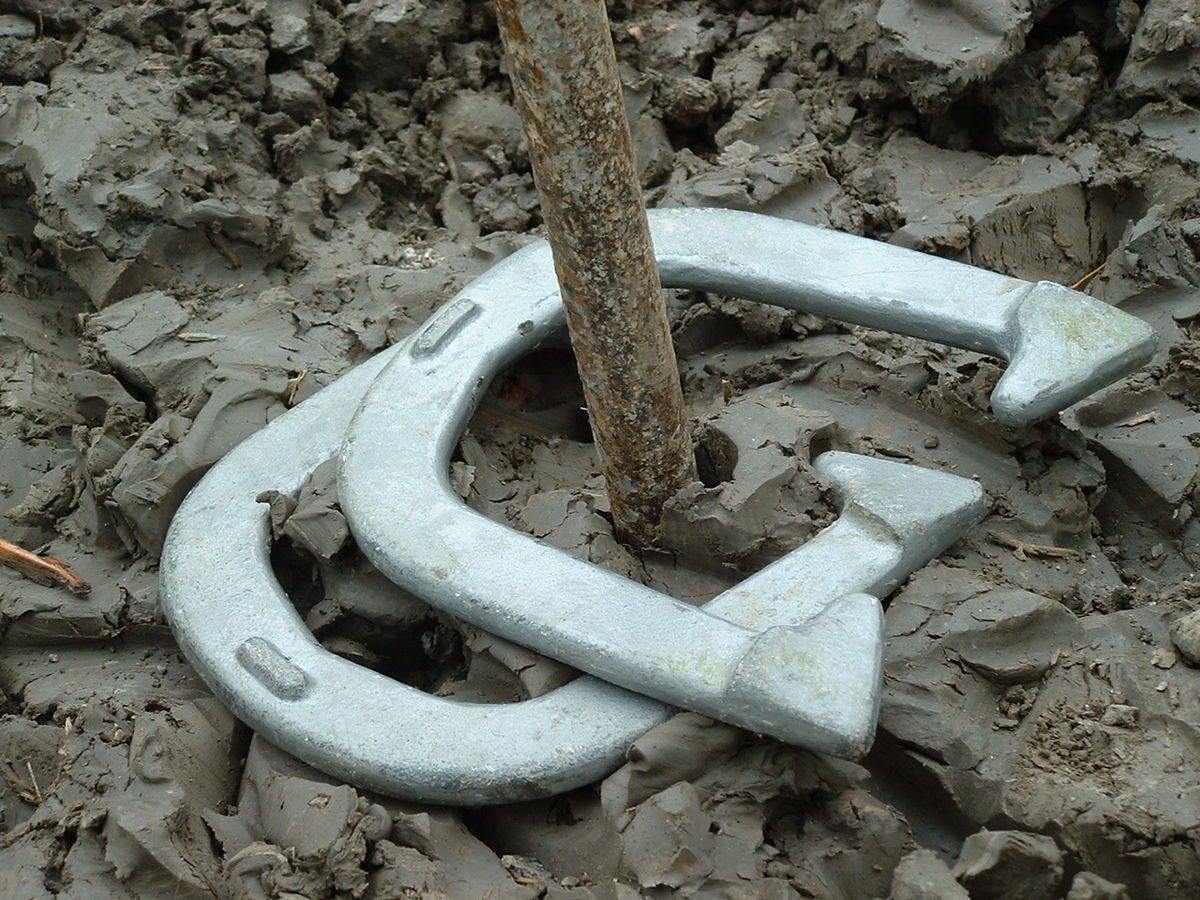
\includegraphics[width=0.5\textwidth,height=\textheight]{img/horseshoes.jpeg}

Keep in mind that your model has a lot to say about what you'll be able
to say at the feature level. As an example, as we get into machine
learning models, you won't have as easy a time with coefficients and
their confidence intervals. For now we'll stop here, but there is a lot
more to the story when it comes to feature level interpretation, and
we'll continue to return to the topic. But first, let's take a look at
interpreting things in another way.

\subsection{Is it a Good Model?}\label{is-it-a-good-model}

Thus far, we've focused on interpretation at the feature level. But
knowing the interpretation of a feature doesn't do you much good if the
model itself is poor! In that case, we also need to assess the model as
a whole, and as with the feature level, we can do this in a few ways.
Before getting too carried away with asking whether your model is any
good or not, you always need to ask your self \emph{relative to what}?
Many model claim top performance, but are statistically
indistinguishable from many other models. So we need to be careful about
how we assess our model, and what we compare it to.

First, we can start with the predictions of our model. As noted
previously, how well the predictions and target line up is a measure of
how well the model fits the data. Most model-level interpretation
involves assessing and comparing model fit and variations on this theme.
One of the better ways to assess model fit is visually, so let's look at
our predictions vs.~the target.

\subsubsection{R}

\begin{Shaded}
\begin{Highlighting}[]
\NormalTok{predictions }\OtherTok{=} \FunctionTok{predict}\NormalTok{(model\_reviews)}
\NormalTok{y }\OtherTok{=}\NormalTok{ df\_reviews}\SpecialCharTok{$}\NormalTok{rating}
\end{Highlighting}
\end{Shaded}

\subsubsection{Python}

\begin{Shaded}
\begin{Highlighting}[]
\NormalTok{predictions }\OperatorTok{=}\NormalTok{ model\_reviews.predict()}
\NormalTok{y }\OperatorTok{=}\NormalTok{ df\_reviews.rating}
\end{Highlighting}
\end{Shaded}

\begin{figure}

{\centering 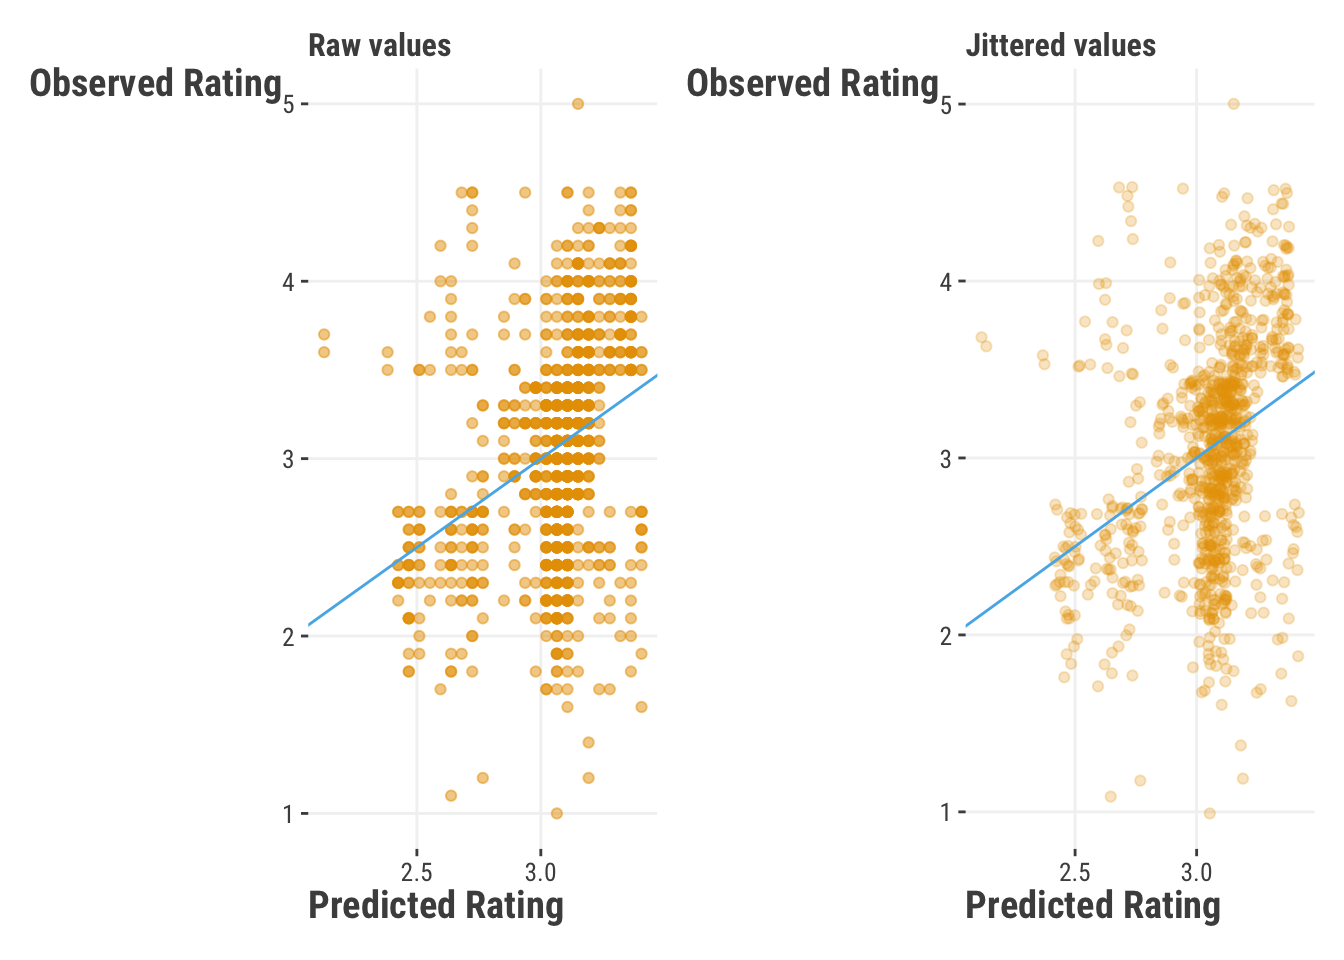
\includegraphics{linear_models_files/figure-pdf/fig-pp-scatter-1.pdf}

}

\caption{\label{fig-pp-scatter}Predictions vs.~Observed Ratings}

\end{figure}

The one on the left is using the raw target and predictions- very
stripey! The reason is that our ratings are only at the single decimal
place precision, and our word count is at the integer level precision,
so we have a lot of ties. The right side jitters the data randomly a bit
so we can see a better pattern, but is otherwise the same. In general,
the closer to a line this plot becomes the better, so we can tell
already there is still a lot of noise left to explain beyond our model.

\subsubsection{Model Metrics}\label{model-metrics}

We've already discussed mean-squared error\footnote{Any time we're
  talking about MSE, we're also talking about RMSE, but MSE is one less
  word/letter so will usually be our default.}, but there are other
metrics we can use to assess \textbf{model fit}. As we noted, (R)MSE is
a very popular measure for continuous targets, telling us the standard
deviation of errors, or how much they bounce around on average. In our
case, the value was 0.59. Another metric we can use in this particular
situation is the mean absolute error, which is similar to the mean
squared error, but instead of squaring the errors, we just take the
absolute value. Conceptually it attempts to get at the same idea, how
much our predictions miss on average, and here the value is 0.46, which
we actually showed in our initial residual plot @fig-residuals-plot.
With either metric, the closer to zero the better, since as we get
closer, we are reducing error.

We can also look at the \textbf{R-squared} (R\textsuperscript{2})value
of the model. R\textsuperscript{2} is possibly the most popular measure
of model performance with linear regression and linear models in
general. Before squaring, it's just the correlation of the values that
we saw in the previous plot (Figure~\ref{fig-pp-scatter}). When we
square it, we can interpret it as a measure of how much of the variance
in the target is explained by the model. In this case, our model shows
the R\textsuperscript{2} is 0.12, which is pretty good for a single
feature model. We interpret it that 12\% of the target is explained by
our model. In addition, we can also interpret R\textsuperscript{2} as 1
- the prorportion of error varaince in the target, which we can
calculate as \(1 - \frac{\textrm{MSE}}{var(y)}\). In other words the
complement of R\textsuperscript{2} is the proportion of the variance in
the target that is not explained by the model. Either way, our result
suggests there is plenty of work left to do!

Note also, that with R\textsuperscript{2} we get a sense of the variance
shared between \emph{all} features in the model and the target, however
complex the model gets. As long as we use it descriptively as a simple
correspondence assessment of our predictions and target, it's a fine
metric. For various reasons, it's not a great metric for comparing
models to each other, but again, as long as you don't get carried away,
it's fine.

\subsection{Prediction
vs.~Explanation}\label{prediction-vs.-explanation}

In your humble authors' views, one can't stress enough the importance of
a model's ability to predict the target. It can be a poor model, maybe
because the data is not great, or we're exploring a new area, but we'll
always be interested in how well a model \textbf{fits} the observed
data, and predicts new data.

Even to this day, \textbf{statistical significance} is focused on a
great deal, even to the point that a much hullabaloo is made about
models that have no predictive power at all. As strange as it may sound,
you can read whole journal articles, news articles, and business reports
in many fields with hardly any mention of prediction. The focus is
almost entirely on the \textbf{explanation} of the model, and usually
the statistical significance of the features. In those settings,
statistical significance is often used as a proxy for importance, which
it never should be. Unfortunately, it is affected by other things
besides the size of the coefficient, and without an understanding of the
context of the features (like how long typical reviews are, what their
range is, what variability of ratings is, etc.), the information it
provides is extremely limited, and many would argue, not even useful at
all. If we are very interested in the coefficient, it is better to focus
on the range of possible values, which is provided by the
\textbf{confidence interval}. While a confidence interval is also a
loaded description of a feature's relationship to the target, we can use
it in a very practical way as a range of possible values for that
weight, and more importantly, think of possibilities rather than
certainties.

Suffice it to say at this point that how much one focuses on prediction
vs.~explanation depends on the context and goals of the data endeavor.
There are cases where predictive capability is of utmost importance, and
we care less about about explanatory details, but not to the point of
ignoring it. For example, even with deep learning models for image
classification, where the inputs are just RGB values, we'd still like to
know what the (notably complex) model is picking up on, otherwise we may
be classifying images based on background nonsense. In some business
settings, we are very or even mostly interested in the
coefficients/weights, which might indicate how to allocate resources in
some fashion, but if they come from a model with no predictive power,
this may be a fruitless endeavor.

In the end we'll need to balance our efforts to suit the task at hand.
Prediction and explanation are both fundamental to the modeling
endeavor.

\section{Adding Complexity}\label{adding-complexity}

We've seen how to fit a model with a single feature and interpret the
results, and that helps us to get oriented to the process. However,
we'll always have more than one feature for a model except under some
very specific circumstances, such as exploratory data analysis. So let's
see how we can do that with a model that makes more sense.

\subsection{Multiple Features}\label{multiple-features}

We can add more features to our model very simply. Using the standard
functions we've already demonstrated, we just add them to the formula
(both R and statsmodels) as follows.

\begin{Shaded}
\begin{Highlighting}[]
\CommentTok{\textquotesingle{}y \textasciitilde{} feature\_1 + feature\_2 + feature\_3\textquotesingle{}}
\end{Highlighting}
\end{Shaded}

In other cases, additional features will just be the additional input
columns. We might have a lot of features, and even for linear models
this could be dozens in some scenarios. A compact depiction of our model
uses the matrix representation, which we'll show in the callout below,
and you can find more detail in the \hyperref[matrix]{matrix section}
overview. For our purposes, all you really need to know is that this:

\begin{equation}\protect\hypertarget{eq-lm-XB}{}{
y = X\beta\qquad  \textrm{or}\qquad y = \alpha + X\beta
}\label{eq-lm-XB}\end{equation}

is the same as this:

\[
y = \alpha + \beta_1 x_1 + \beta_2 x_2 + \beta_3 x_3 \dots
\]

where \(X\) is a matrix of features\footnote{For linear regression as we
  estimate it here, there is actually an additional column at the
  beginning of the matrix that is all ones, which is a way to
  incorporate the intercept. However, most models that use a matrix as
  input will not have the intercept column, as it's not part of the
  model estimation or is estimated separately.}, and \(\beta\) is a
vector of coefficients. Matrix multiplication allows us an efficient way
to get our expected value/prediction.

\begin{tcolorbox}[enhanced jigsaw, rightrule=.15mm, opacityback=0, left=2mm, bottomrule=.15mm, toprule=.15mm, arc=.35mm, colframe=quarto-callout-note-color-frame, leftrule=.75mm, breakable, colback=white]

\textbf{Matrix Representation of a Linear Model}\vspace{2mm}

Here we'll show the matrix representation form of the linear model, for
the typical case where we have more than one feature in the model. In
the following, y is a vector of all target observations, and likewise
each x is a (row) vector of all observations for that feature. The b
vector is the vector of coefficients. The 1 serves as a means to
incorporate the intercept. It's just a feature that always has a value
of 1. The matrix multiplication is just a compact way of expressing the
sum of the features multiplied by their coefficients. We can even do it
more

Here is y as a vector of observations, n x 1.

\begin{equation}\protect\hypertarget{eq-lm-mat-y}{}{
\textbf{y} = \begin{bmatrix}
y_1 \\
y_2 \\
\vdots \\
y_n
\end{bmatrix}
}\label{eq-lm-mat-y}\end{equation}

Here is the vector for x, including the intercept:

\begin{equation}\protect\hypertarget{eq-lm-mat-x}{}{
\textbf{X} = \begin{bmatrix}
1 & x_{11} & x_{12} & \dots & x_{1p} \\
1 & x_{21} & x_{22} & \dots & x_{2p} \\
\vdots & \vdots & \vdots & \ddots & \vdots \\
1 & x_{n1} & x_{n2} & \dots & x_{np}
\end{bmatrix}
}\label{eq-lm-mat-x}\end{equation}

And finally, here is the vector of coefficients:

\begin{equation}\protect\hypertarget{eq-lm-mat-b}{}{
\textbf{b} = \begin{bmatrix}
b_0 \\
b_1 \\
\vdots \\
b_p
\end{bmatrix}
}\label{eq-lm-mat-b}\end{equation}

Putting it all together, we get the linear model in matrix form:

\begin{equation}\protect\hypertarget{eq-lm-mat-mult}{}{
\textbf{y = Xb }
}\label{eq-lm-mat-mult}\end{equation}

\end{tcolorbox}

With that in mind, let's get to our model! In what follows, we keep the
word count, but now we add some aspects of the reviewer, such as age and
the number of children in the household, features related to the movie-
the release year, the length of the movie in minutes, and the total
reviews received. We'll also add another review level feature- the year
the review was written. We'll use the same approach as before, and
literally just add them as we depicted in our linear model formula
(Equation~\ref{eq-lm-basic}).

\subsubsection{R}

\begin{Shaded}
\begin{Highlighting}[]
\NormalTok{model\_reviews\_extra }\OtherTok{=} \FunctionTok{lm}\NormalTok{(}
\NormalTok{    rating }\SpecialCharTok{\textasciitilde{}}
\NormalTok{        word\_count}
        \SpecialCharTok{+}\NormalTok{ age}
        \SpecialCharTok{+}\NormalTok{ review\_year}
        \SpecialCharTok{+}\NormalTok{ release\_year}
        \SpecialCharTok{+}\NormalTok{ length\_minutes}
        \SpecialCharTok{+}\NormalTok{ children\_in\_home}
        \SpecialCharTok{+}\NormalTok{ total\_reviews,}
    \AttributeTok{data =}\NormalTok{ df\_reviews}
\NormalTok{)}

\FunctionTok{summary}\NormalTok{(model\_reviews\_extra)}
\end{Highlighting}
\end{Shaded}

\begin{verbatim}

Call:
lm(formula = rating ~ word_count + age + review_year + release_year + 
    length_minutes + children_in_home + total_reviews, data = df_reviews)

Residuals:
    Min      1Q  Median      3Q     Max 
-1.8231 -0.3399  0.0107  0.3566  1.5144 

Coefficients:
                  Estimate Std. Error t value Pr(>|t|)    
(Intercept)      -4.56e+01   7.46e+00   -6.11  1.5e-09 ***
word_count       -3.03e-02   3.33e-03   -9.10  < 2e-16 ***
age              -1.69e-03   9.24e-04   -1.83   0.0683 .  
review_year       9.88e-03   3.23e-03    3.05   0.0023 ** 
release_year      1.33e-02   1.79e-03    7.43  2.3e-13 ***
length_minutes    1.67e-02   1.53e-03   10.90  < 2e-16 ***
children_in_home  1.03e-01   2.54e-02    4.05  5.5e-05 ***
total_reviews     7.62e-05   6.16e-06   12.36  < 2e-16 ***
---
Signif. codes:  0 '***' 0.001 '**' 0.01 '*' 0.05 '.' 0.1 ' ' 1

Residual standard error: 0.52 on 992 degrees of freedom
Multiple R-squared:  0.321, Adjusted R-squared:  0.316 
F-statistic:   67 on 7 and 992 DF,  p-value: <2e-16
\end{verbatim}

\subsubsection{Python}

\begin{Shaded}
\begin{Highlighting}[]
\NormalTok{model\_reviews\_extra }\OperatorTok{=}\NormalTok{ smf.ols(}
\NormalTok{    formula }\OperatorTok{=} \StringTok{\textquotesingle{}rating \textasciitilde{} word\_count + age + review\_year + release\_year + length\_minutes + children\_in\_home + total\_reviews\textquotesingle{}}\NormalTok{,}
\NormalTok{    data }\OperatorTok{=}\NormalTok{ df\_reviews}
\NormalTok{).fit()}

\NormalTok{model\_reviews\_extra.summary(slim }\OperatorTok{=} \VariableTok{True}\NormalTok{)}
\end{Highlighting}
\end{Shaded}

\begin{verbatim}
<class 'statsmodels.iolib.summary.Summary'>
"""
                            OLS Regression Results                            
==============================================================================
Dep. Variable:                 rating   R-squared:                       0.321
Model:                            OLS   Adj. R-squared:                  0.316
No. Observations:                1000   F-statistic:                     67.02
Covariance Type:            nonrobust   Prob (F-statistic):           3.73e-79
====================================================================================
                       coef    std err          t      P>|t|      [0.025      0.975]
------------------------------------------------------------------------------------
Intercept          -45.5688      7.463     -6.106      0.000     -60.215     -30.923
word_count          -0.0303      0.003     -9.102      0.000      -0.037      -0.024
age                 -0.0017      0.001     -1.825      0.068      -0.004       0.000
review_year          0.0099      0.003      3.055      0.002       0.004       0.016
release_year         0.0133      0.002      7.434      0.000       0.010       0.017
length_minutes       0.0167      0.002     10.897      0.000       0.014       0.020
children_in_home     0.1028      0.025      4.051      0.000       0.053       0.153
total_reviews     7.616e-05   6.16e-06     12.362      0.000    6.41e-05    8.83e-05
====================================================================================

Notes:
[1] Standard Errors assume that the covariance matrix of the errors is correctly specified.
[2] The condition number is large, 2.82e+06. This might indicate that there are
strong multicollinearity or other numerical problems.
"""
\end{verbatim}

There is definitely more to unpack here but it's important to note that
it's just \emph{more} stuff, not different stuff. The model-level
components are the same in that we still see R\textsuperscript{2} etc.,
although they are all `better' (higher R\textsuperscript{2}, lower
error) because we have a more predictive model. Our coefficents look the
same also, and the fact is we'd interpret the in the same way. Starting
with word count, we see that it's still statistically significant, but
it has been reduced just slightly from our previous model where it was
the only feature (-0.04 vs.~-0.03). Why? This suggests that word count
has some non-zero correlation, sometimes called \textbf{collinearity},
with other features that are also explaining the target to some extent.
Our linear model shows the effect of each feature \emph{controlling for
other features}, or, \emph{holding other features constant}\footnote{A
  lot of statisticians and causal modeling folks get very hung up on the
  terminology here, but we'll leave that to them as we'd like to get on
  with things. For our purposes, we'll just say that we're interested in
  the effect of a feature \emph{after} we've accounted for the other
  features in the model.}. Conceptually this means that the effect of
word count is the effect of word count \emph{after} we've accounted for
the other features in the model. In this case, an increase of a single
word results in a -0.03 drop. Looking at another feature, the addition
of a child to the home is associated with 0.1 bump in rating, accounting
for the other features.

Thinking about prediction, how would we get a prediction for a movie
rating with a review that is 12 words long, written in 2020, by a 30
year old with one child, for a movie that is 100 minutes long, released
in 2015, with 10000 total reviews? Conceptually we just plug in the
values for each feature into the model equation exactly as we did for a
single feature. But since that'd be tedious, we'll just use the
\texttt{predict} function, which is a bit easier and what we'd normally
do.

\subsubsection{R}

\begin{Shaded}
\begin{Highlighting}[]
\NormalTok{predict\_observation }\OtherTok{=} \FunctionTok{tibble}\NormalTok{(}
    \AttributeTok{word\_count =} \DecValTok{12}\NormalTok{,}
    \AttributeTok{age =} \DecValTok{30}\NormalTok{,}
    \AttributeTok{children\_in\_home =} \DecValTok{1}\NormalTok{,}
    \AttributeTok{review\_year =} \DecValTok{2020}\NormalTok{,}
    \AttributeTok{release\_year =} \DecValTok{2015}\NormalTok{,}
    \AttributeTok{length\_minutes =} \DecValTok{100}\NormalTok{,}
    \AttributeTok{total\_reviews =} \DecValTok{10000}
\NormalTok{)}

\FunctionTok{predict}\NormalTok{(}
\NormalTok{    model\_reviews\_extra,}
    \AttributeTok{newdata =}\NormalTok{ predict\_observation}
\NormalTok{)}
\end{Highlighting}
\end{Shaded}

\begin{verbatim}
   1 
3.26 
\end{verbatim}

\subsubsection{Python}

\begin{Shaded}
\begin{Highlighting}[]
\NormalTok{predict\_observation }\OperatorTok{=}\NormalTok{ pd.DataFrame(}
\NormalTok{    \{}
        \StringTok{\textquotesingle{}word\_count\textquotesingle{}}\NormalTok{: }\DecValTok{12}\NormalTok{,}
        \StringTok{\textquotesingle{}age\textquotesingle{}}\NormalTok{: }\DecValTok{30}\NormalTok{,}
        \StringTok{\textquotesingle{}children\_in\_home\textquotesingle{}}\NormalTok{: }\DecValTok{1}\NormalTok{,}
        \StringTok{\textquotesingle{}review\_year\textquotesingle{}}\NormalTok{: }\DecValTok{2020}\NormalTok{,}
        \StringTok{\textquotesingle{}release\_year\textquotesingle{}}\NormalTok{: }\DecValTok{2015}\NormalTok{,}
        \StringTok{\textquotesingle{}length\_minutes\textquotesingle{}}\NormalTok{: }\DecValTok{100}\NormalTok{,}
        \StringTok{\textquotesingle{}total\_reviews\textquotesingle{}}\NormalTok{: }\DecValTok{10000}
\NormalTok{    \},}
\NormalTok{    index }\OperatorTok{=}\NormalTok{ [}\StringTok{\textquotesingle{}new\_observation\textquotesingle{}}\NormalTok{]}
\NormalTok{)}

\NormalTok{model\_reviews\_extra.predict(predict\_observation)}
\end{Highlighting}
\end{Shaded}

\begin{verbatim}
new_observation    3.2595
dtype: float64
\end{verbatim}

In our example we're just getting a single prediction, but don't let
that hold you back! You can predict an entire data set if you want, and
use any values for the features you want. We'll do this explicitly in
the \hyperref[machine-learning]{machine learning chapter}, but for now,
try getting a prediction for a different set of values.

\subsection{More Interpretation Tools}\label{more-interpretation-tools}

\subsubsection{SHAP Values}\label{shap-values}

Some models are more complicated than can be explained by a simple
coefficient, e.g.~nonlinear effects in generalized additive models, or
may not even have feature-specific coefficients, like gradient boosting
models, or may have many parameters associated with a feature, as in
deep learning. Such models typically won't come with statistical output
like standard errors and confidence intervals either. But we'll still
have some tricks up our sleeve to help us figure things out!

A very common interpretation tool is called a \textbf{SHAP value}. SHAP
stands for \textbf{SHapley Additive exPlanations}, and it provides a
means to understand how much each feature contributes to a specific
prediction. It's based on a concept from game theory called the
\textbf{Shapley value}, which is a way to understand how much each
player contributes to the outcome of a game. The reason we bring it up
here is that it is has a nice intuition in the linear model case, and
demonstrating now is a good way to get a sense of how it works. While
the actual computations can be tedious, the basic idea is relatively
straightforward- for a given prediction at a specific observation with
set feature values, we can calculate the difference between the
prediction at that observation and the average prediction. This is the
\textbf{local effect} of the feature. However, we must also consider
doing this for all possible values of other features that might be in a
model, as well as considering whether other features are present for the
prediction or not. The initial Shapley approach is to average the local
effects over all possible combinations of features, which is
computationally intractable for all but the simplest models. The SHAP
approach offers more computationally feasible methods for estimation
which, while still computationally intensive, is doable for many models.
The SHAP approach also has the benefit of being able to be applied to
\emph{any} model, and it's the approach we'll use here and return to
with some of our other models.

Let's look at the SHAP values for our model. We'll start with a single
feature value/observation, using our multifeature model. Here we'll use
the first observation where there are 12 words for word count, age of
reviewer is 30, a movie length of 100 minutes etc. To aid our
understanding, we calculate the shap value related to word count at that
observation by hand, and using a package.

\subsubsection{R}

\begin{Shaded}
\begin{Highlighting}[]
\CommentTok{\# first we need to get the average prediction}
\NormalTok{avg\_pred }\OtherTok{=} \FunctionTok{mean}\NormalTok{(}\FunctionTok{predict}\NormalTok{(model\_reviews\_extra))}


\CommentTok{\# then we need to get the prediction for the feature value of interest}
\CommentTok{\# for all observations, and average them}
\NormalTok{pred\_observation }\OtherTok{=} \FunctionTok{predict}\NormalTok{(}
\NormalTok{    model\_reviews\_extra,}
    \AttributeTok{newdata =}\NormalTok{ df\_reviews }\SpecialCharTok{|\textgreater{}} \FunctionTok{mutate}\NormalTok{(}\AttributeTok{word\_count =} \DecValTok{12}\NormalTok{)}
\NormalTok{)}

\CommentTok{\# then we can calculate the shap value}
\NormalTok{shap\_value }\OtherTok{=} \FunctionTok{mean}\NormalTok{(pred\_observation) }\SpecialCharTok{{-}}\NormalTok{ avg\_pred}

\CommentTok{\# we can also use the DALEX package to do this for us}
\NormalTok{explainer }\OtherTok{=}\NormalTok{ DALEX}\SpecialCharTok{::}\FunctionTok{explain}\NormalTok{(model\_reviews\_extra, }\AttributeTok{verbose =} \ConstantTok{FALSE}\NormalTok{)}

\CommentTok{\# observation of interest we want shap values for}
\NormalTok{obs\_of\_interest }\OtherTok{=} \FunctionTok{tibble}\NormalTok{(}
    \AttributeTok{word\_count =} \DecValTok{12}\NormalTok{,}
    \AttributeTok{age =} \DecValTok{30}\NormalTok{,}
    \AttributeTok{children\_in\_home =} \DecValTok{1}\NormalTok{,}
    \AttributeTok{length\_minutes =} \DecValTok{100}\NormalTok{,}
    \AttributeTok{total\_reviews =} \DecValTok{10000}\NormalTok{,}
    \AttributeTok{release\_year =} \DecValTok{2015}\NormalTok{,}
    \AttributeTok{review\_year =} \DecValTok{2020}\NormalTok{,}
\NormalTok{)}

\NormalTok{shap\_value\_package }\OtherTok{=}\NormalTok{ DALEX}\SpecialCharTok{::}\FunctionTok{predict\_parts}\NormalTok{(}
\NormalTok{    explainer,}
\NormalTok{    obs\_of\_interest,}
    \AttributeTok{type =} \StringTok{"shap"}
\NormalTok{)}
\end{Highlighting}
\end{Shaded}

\subsubsection{Python}

\begin{Shaded}
\begin{Highlighting}[]
\CommentTok{\# first we need to get the average prediction}
\NormalTok{avg\_pred }\OperatorTok{=}\NormalTok{ model\_reviews\_extra.predict(df\_reviews).mean()}

\CommentTok{\# then we need to get the prediction for the feature value of interest}
\NormalTok{pred\_observation }\OperatorTok{=}\NormalTok{ model\_reviews\_extra.predict(df\_reviews.assign(word\_count }\OperatorTok{=} \DecValTok{12}\NormalTok{))}

\CommentTok{\# then we can calculate the shap value}
\NormalTok{shap\_value }\OperatorTok{=}\NormalTok{ pred\_observation.mean() }\OperatorTok{{-}}\NormalTok{ avg\_pred}


\CommentTok{\# now use the shap package for this; it does not work with statsmodels though,}
\CommentTok{\# and single feature models are a bit cumbersome, but we still get there in the end!}
\ImportTok{import}\NormalTok{ shap}
\ImportTok{from}\NormalTok{ sklearn.linear\_model }\ImportTok{import}\NormalTok{ LinearRegression}

\CommentTok{\# set data up for shap and sklearn}
\NormalTok{fnames }\OperatorTok{=}\NormalTok{ [}\StringTok{\textquotesingle{}word\_count\textquotesingle{}}\NormalTok{, }\StringTok{\textquotesingle{}age\textquotesingle{}}\NormalTok{, }\StringTok{\textquotesingle{}review\_year\textquotesingle{}}\NormalTok{, }\StringTok{\textquotesingle{}release\_year\textquotesingle{}}\NormalTok{, }\StringTok{\textquotesingle{}length\_minutes\textquotesingle{}}\NormalTok{, }\StringTok{\textquotesingle{}children\_in\_home\textquotesingle{}}\NormalTok{, }\StringTok{\textquotesingle{}total\_reviews\textquotesingle{}}\NormalTok{]}

\NormalTok{X }\OperatorTok{=}\NormalTok{ df\_reviews[fnames]}
\NormalTok{y }\OperatorTok{=}\NormalTok{ df\_reviews[}\StringTok{\textquotesingle{}rating\textquotesingle{}}\NormalTok{]}

\CommentTok{\# use a linear model that works with shap}
\NormalTok{model\_reviews }\OperatorTok{=}\NormalTok{ LinearRegression().fit(X, y)}

\CommentTok{\# 1000 instances for use as the \textquotesingle{}background distribution\textquotesingle{}}
\NormalTok{X\_sample }\OperatorTok{=}\NormalTok{ shap.maskers.Independent(data }\OperatorTok{=}\NormalTok{ X, max\_samples }\OperatorTok{=} \DecValTok{1000}\NormalTok{)  }

\CommentTok{\# \# compute the SHAP values for the linear model}
\NormalTok{explainer\_linear }\OperatorTok{=}\NormalTok{ shap.Explainer(}
\NormalTok{    model\_reviews.predict, }
\NormalTok{    X\_sample   }
\NormalTok{)}

\CommentTok{\# find an index where word\_count is 12}
\NormalTok{obs\_of\_interest }\OperatorTok{=}\NormalTok{ pd.DataFrame(\{}
    \StringTok{\textquotesingle{}word\_count\textquotesingle{}}\NormalTok{: }\DecValTok{12}\NormalTok{,}
    \StringTok{\textquotesingle{}age\textquotesingle{}}\NormalTok{: }\DecValTok{30}\NormalTok{,}
    \StringTok{\textquotesingle{}children\_in\_home\textquotesingle{}}\NormalTok{: }\DecValTok{1}\NormalTok{,}
    \StringTok{\textquotesingle{}review\_year\textquotesingle{}}\NormalTok{: }\DecValTok{2020}\NormalTok{,}
    \StringTok{\textquotesingle{}release\_year\textquotesingle{}}\NormalTok{: }\DecValTok{2015}\NormalTok{,}
    \StringTok{\textquotesingle{}length\_minutes\textquotesingle{}}\NormalTok{: }\DecValTok{100}\NormalTok{,}
    \StringTok{\textquotesingle{}total\_reviews\textquotesingle{}}\NormalTok{: }\DecValTok{10000}
\NormalTok{\}, index }\OperatorTok{=}\NormalTok{ [}\StringTok{\textquotesingle{}new\_observation\textquotesingle{}}\NormalTok{])}

\NormalTok{shap\_values\_linear }\OperatorTok{=}\NormalTok{ explainer\_linear(obs\_of\_interest)}

\NormalTok{shap\_value }\OperatorTok{=}\NormalTok{ shap\_values\_linear.values[}\DecValTok{0}\NormalTok{, }\DecValTok{0}\NormalTok{]}
\end{Highlighting}
\end{Shaded}

\begin{table}

\caption{\label{tbl-shap-values-comparison}\textbf{?(caption)}}\begin{minipage}[t]{\linewidth}
\subcaption{\label{tbl-shap-values-comparison-1}}

{\centering 

\begin{longtable*}{rr}
\toprule
ours & dalex \\ 
\midrule\addlinespace[2.5pt]
\textcolor[HTML]{404040}{$-0.051$} & \textcolor[HTML]{404040}{$-0.051$} \\ 
\bottomrule
\end{longtable*}

}

\end{minipage}%

\end{table}

So we see the contribution to a prediction for a single feature, but the
shap-related packages provide them for all features, and thus get a
sense of each feature's contribution to the predicion. The following
shows this as a visualization, either a force plot and waterfall plot.
Smaller contributions are aggregated to one effect to simplify the plot.
The dotted line represents the average prediction from our model
(E{[}f(x){]}) and the prediction we have for the observation (f(x)). We
see that total reviews and length in minutes contribute most to the
prediction at this observation, followed by release year. We can also
see that the effect of movie length is negative.

\begin{figure}

{\centering 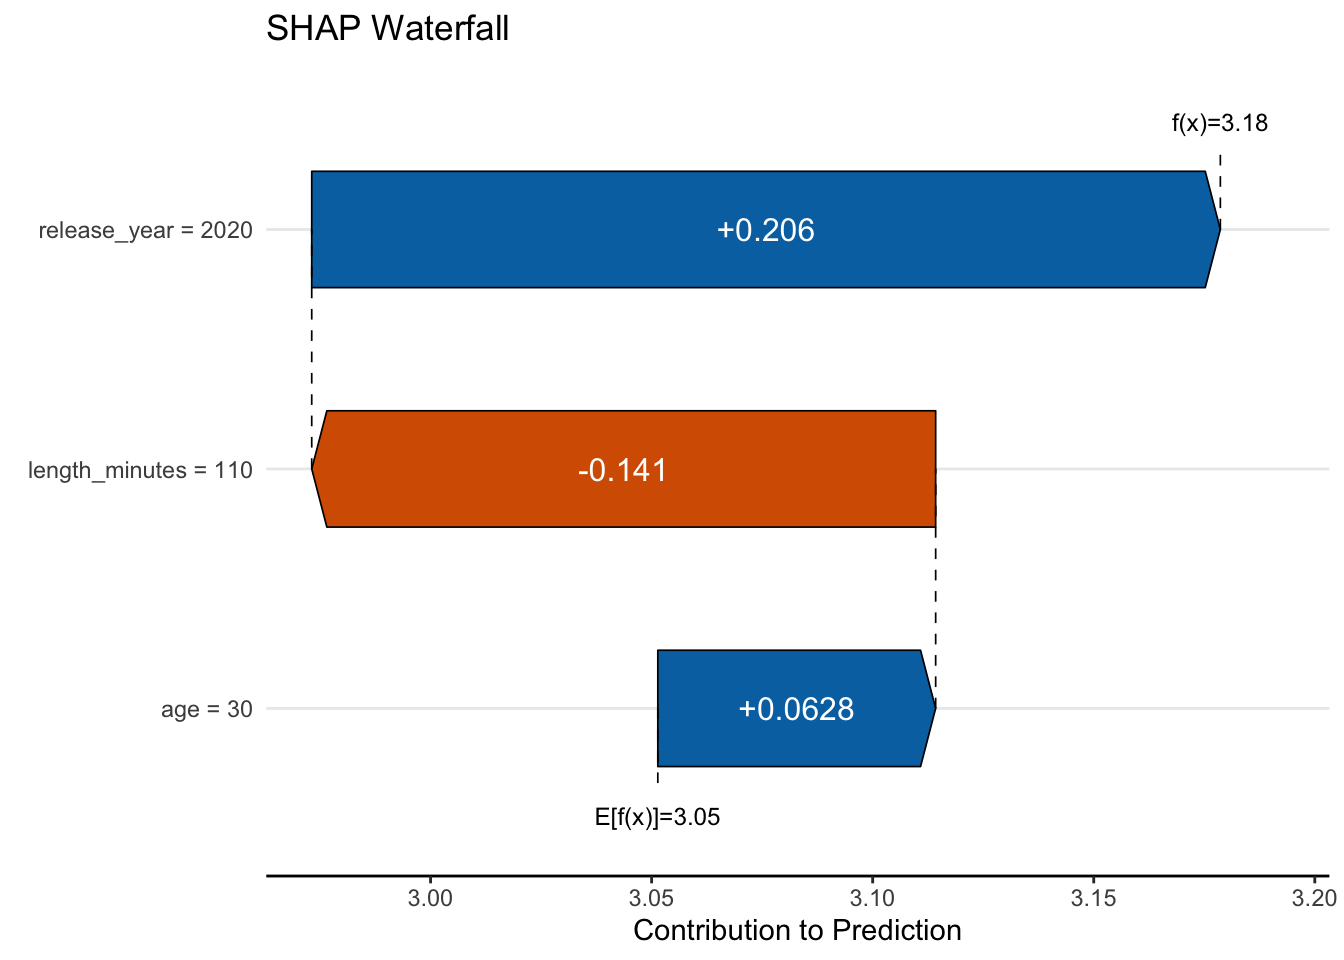
\includegraphics{linear_models_files/figure-pdf/shap-viz-r-1.pdf}

}

\caption{SHAP Visualizations}

\end{figure}

Pretty neat huh? So for any observation we want to, and more
importantly, for any model we might use, we can get a sense of how
features contribute to that prediction. We also can get a sense of how
much each feature contributes to the model as a whole by aggregating
these values across all observations in our data, and this provides a
measure of \textbf{feature importance}, but we'll come back to that in a
bit.

If we are concerned with a single feature's relationship with the
target, we can also look at the \textbf{partial dependence plot} (PDP).
The PDP shows the relationship between a feature and the target, but
averaged over all other features. In other words, it shows the effect of
a feature on the target, but averaged over all other features. For the
linear case, it has a direct correspondence to the shap value. The SHAP
value is the value the difference between the average prediction and the
point on the PDP for a feature at a specific feature value.

We can also look at the \textbf{individual conditional expectation}
(ICE) plot, which is a PDP for a single observation. The PDP is a very
common plot for understanding the relationship between a feature and the
target, and we'll see it again with other models. The ICE plot is less
common, but it's a nice way to see how a feature affects the target for
a single observation.

In addition, there are other plots that are similar to the PDP and ICE,
such as the \textbf{accumulated local effect} (ALE) plot, which is a bit
more robust to correlated features than the PDP plo. Where the PDP and
ICE plots show the average effect of a feature on the target, the ALE
plot focuses on average differences in predictions for the feature at a
specific value versus predictions at feature values nearby, and centers
the result so that the average difference is zero. We'll show all three
here.

https://christophm.github.io/interpretable-ml-book/ (good reference for
all plots)

\begin{figure}

{\centering 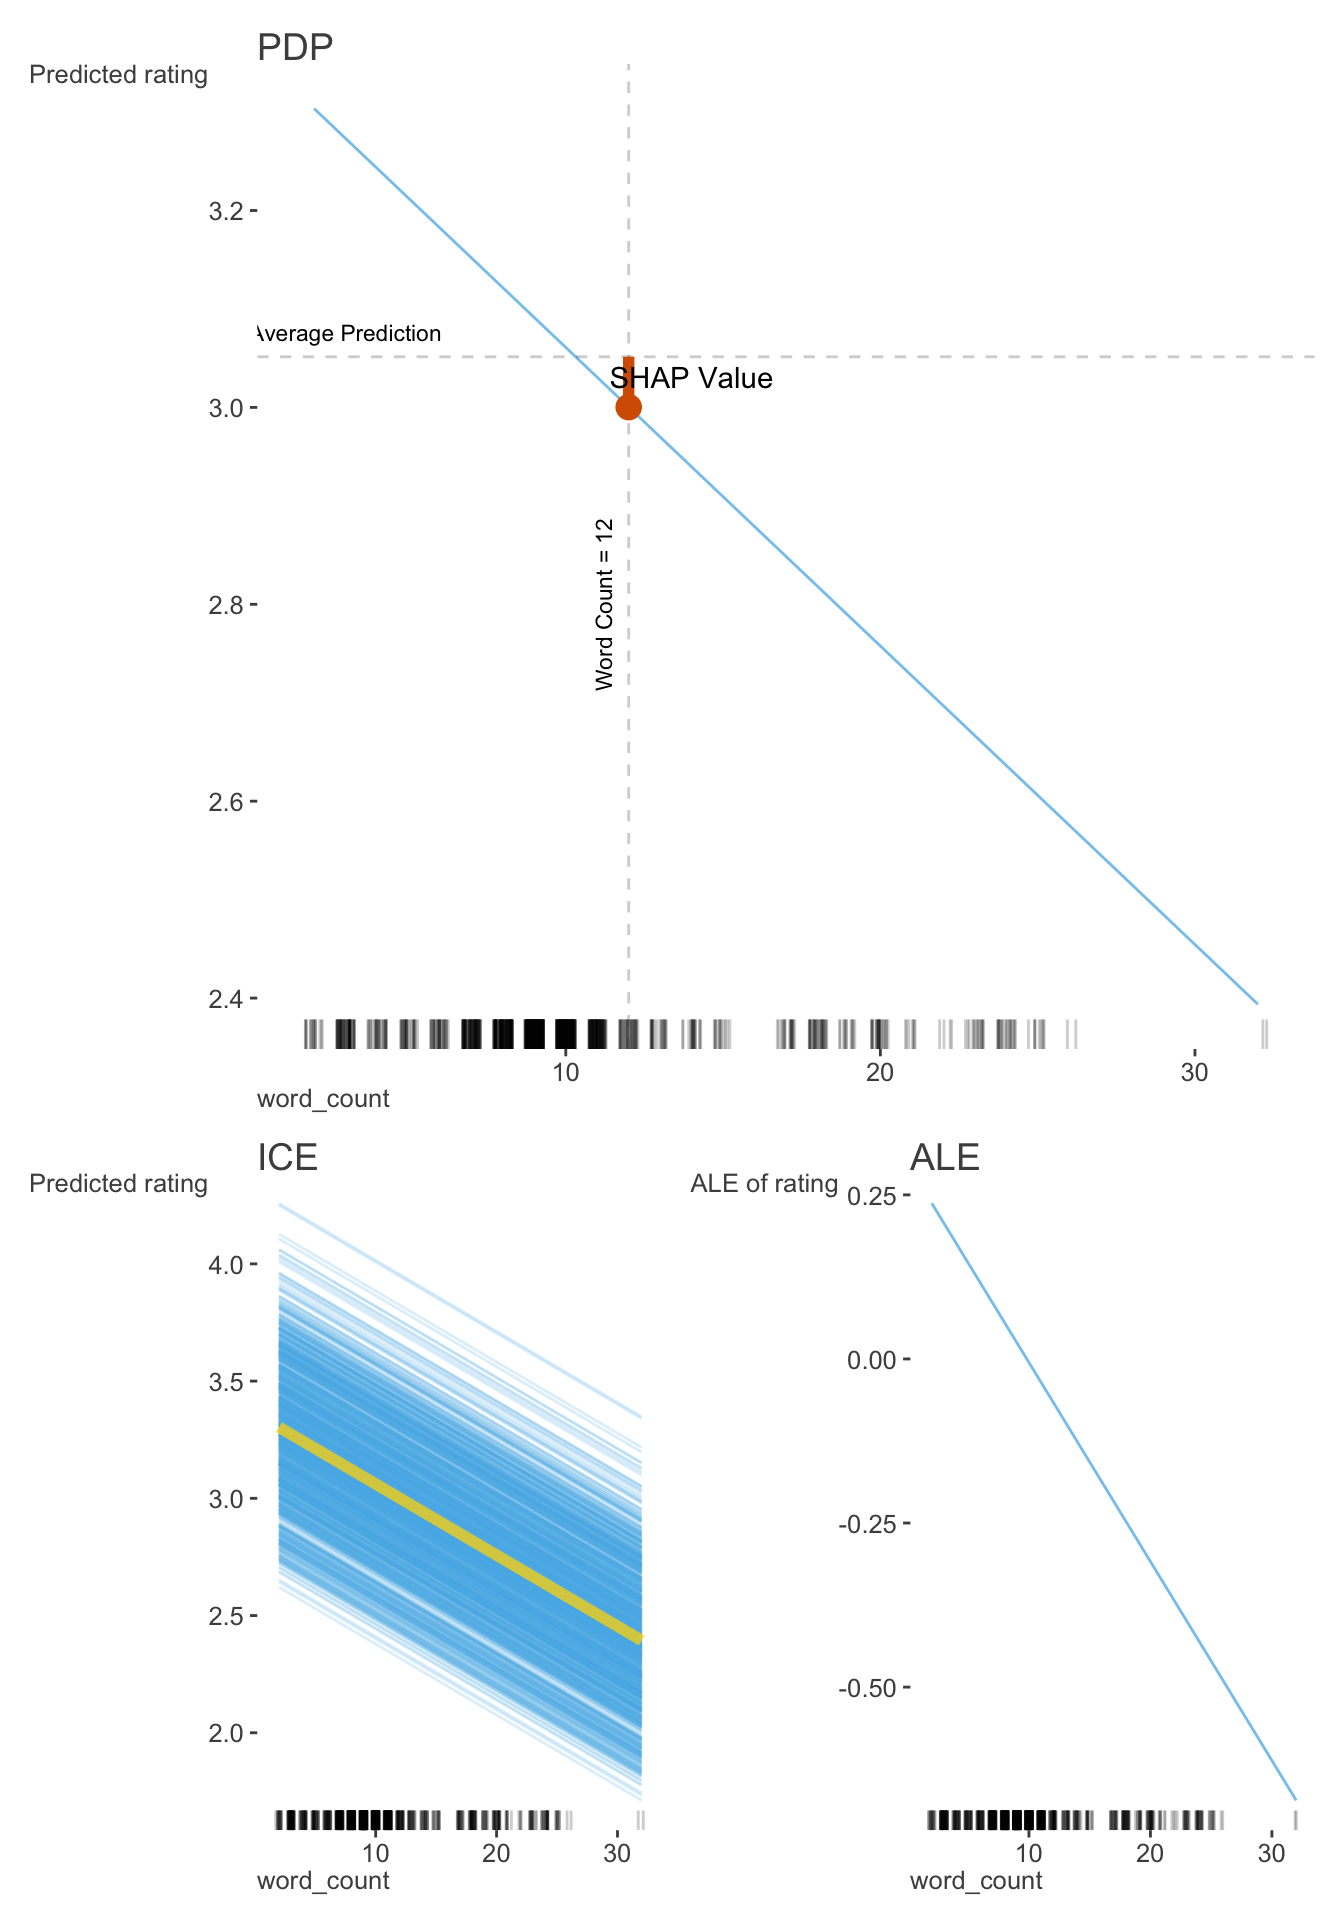
\includegraphics{linear_models_files/figure-pdf/pdp-ice-r-1.pdf}

}

\caption{Partial Dependence and Individual Conditional Expectation
Plots}

\end{figure}

Kinda cool but maybe not so interesting in that they all kind of tell us
the same thing about our negative relationship between word count and
rating, which we already knew from our coefficient value. The real power
will come in later when we use interactions, nonlinear effects, and
other models. But it's good to note now that the PDP, ICE, and ALE plots
are a nice way to get a sense of the relationship between a feature and
the target, and we'll see them again with other models.

\subsection{Feature Importance}\label{feature-importance}

How important is a feature? It's a common question, and one that is
often asked of models, but the answer ranges from `it depends' and `it
doesn't matter'. Let's start with some hard facts:

\begin{itemize}
\tightlist
\item
  There is no single definition of importance.
\item
  There is no single metric for \emph{any} model that will definitively
  tell you how important a feature is relative to others in all
  data/model contexts.
\item
  There are many metrics for a given model that are equally valid, but
  may come to different conclusions.
\item
  Any non-zero feature contribution is potentially `imortant', however
  small.
\item
  Many metrics of importance fail to adequately capture interactions and
  deal with correlated features.
\item
  All measures of importance are measured with uncertainty, and the
  uncertainty can be large.
\item
  Relative to\ldots{} what? A poor model will still have relatively
  `important' features, but they may not be useful.
\item
  It rarely makes sense to drop features based on importance alone, and
  will typically drop performance to do so.
\item
  In the end, what will you do with the information?
\end{itemize}

To show just how difficult measuring feature importance is, we only have
to stick with our simple linear regression. Think again about
R\textsuperscript{2}: it tells us the proportion of the target explained
by our features. An ideal measure of importance would be able to tell us
how much each feature contributes to that proportion, or in other words,
decomposes R\textsuperscript{2} into the relative contributions of each
feature. One of the most common measures of importance in linear models
is the standardized coefficient we demonstrated earlier. You know what
it doesn't do? Decompose R\textsuperscript{2}. The easiest situation we
could hope for with regard to feature importance is the basic linear
model we've been using. Everything is linear, with no interactions, or
other things going on. And yet there are many logical ways to determine
feature importance, and some even break down R\textsuperscript{2}, but
they won't necessarily agree with each other in ranking or relative
differences. If you can get a measure of statistical difference between
whatever metric you choose, it's often the case that `top' features will
not be statistically different from other features. So what do we do?
We'll show a few methods here, but the main point is that there is no
single answer, and it's important to understand what you're trying to do
with the information.

Let's start things off by returning to our SHAP value. If we take the
average absolute shap for each feature, we get a sense of the typical
contribution size for the features. We can then rank order them as
accordingly. Here we see that the most important features here are the
number of reviews and the length of the movie. Note that we can't speak
to direction here, only magnitude. We can also see that word count is
relatively less important.

\begin{figure}

{\centering 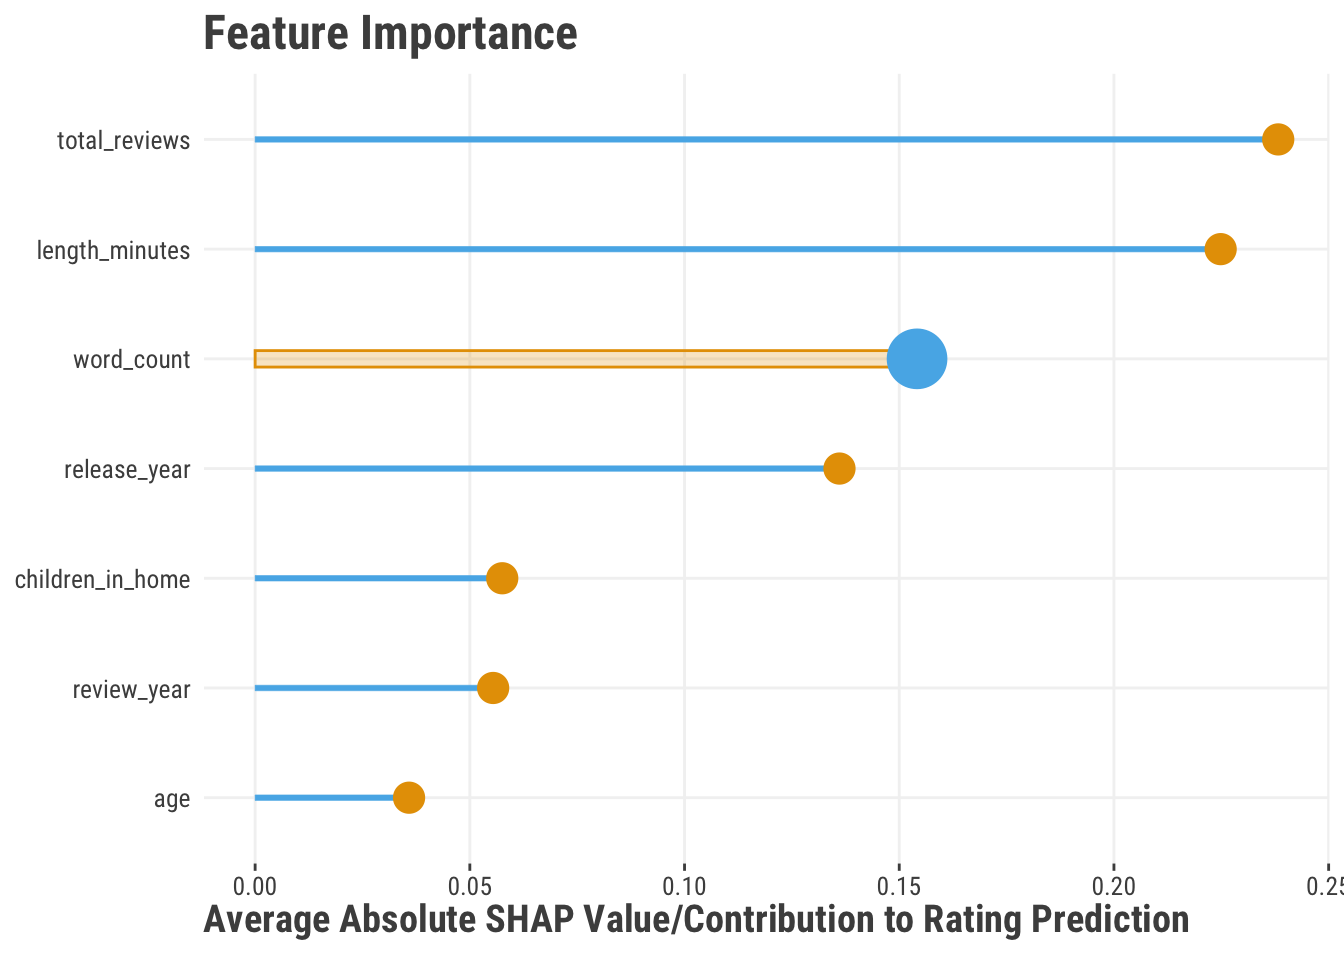
\includegraphics{linear_models_files/figure-pdf/shap-importance-bar-1.pdf}

}

\caption{SHAP Importance}

\end{figure}

Now here are some additional methods, some more reasonable than others,
some which decompose R\textsuperscript{2} and those that do not. Aside
from SHAP, the value represents the proportion of the
R\textsuperscript{2} value that is attributable to the feature. The ones
that truly decompose R\textsuperscript{2} are in agreement for the most
part and seem to think highly of word count. The latter seem to be more
varied, and only SHAP devalues word count, but possibly for good reason.
Which is best? Which is correct? None. But we can get a sense at least
that total reviews and length in minutes are likely useful features to
our model.

\begin{figure}

{\centering 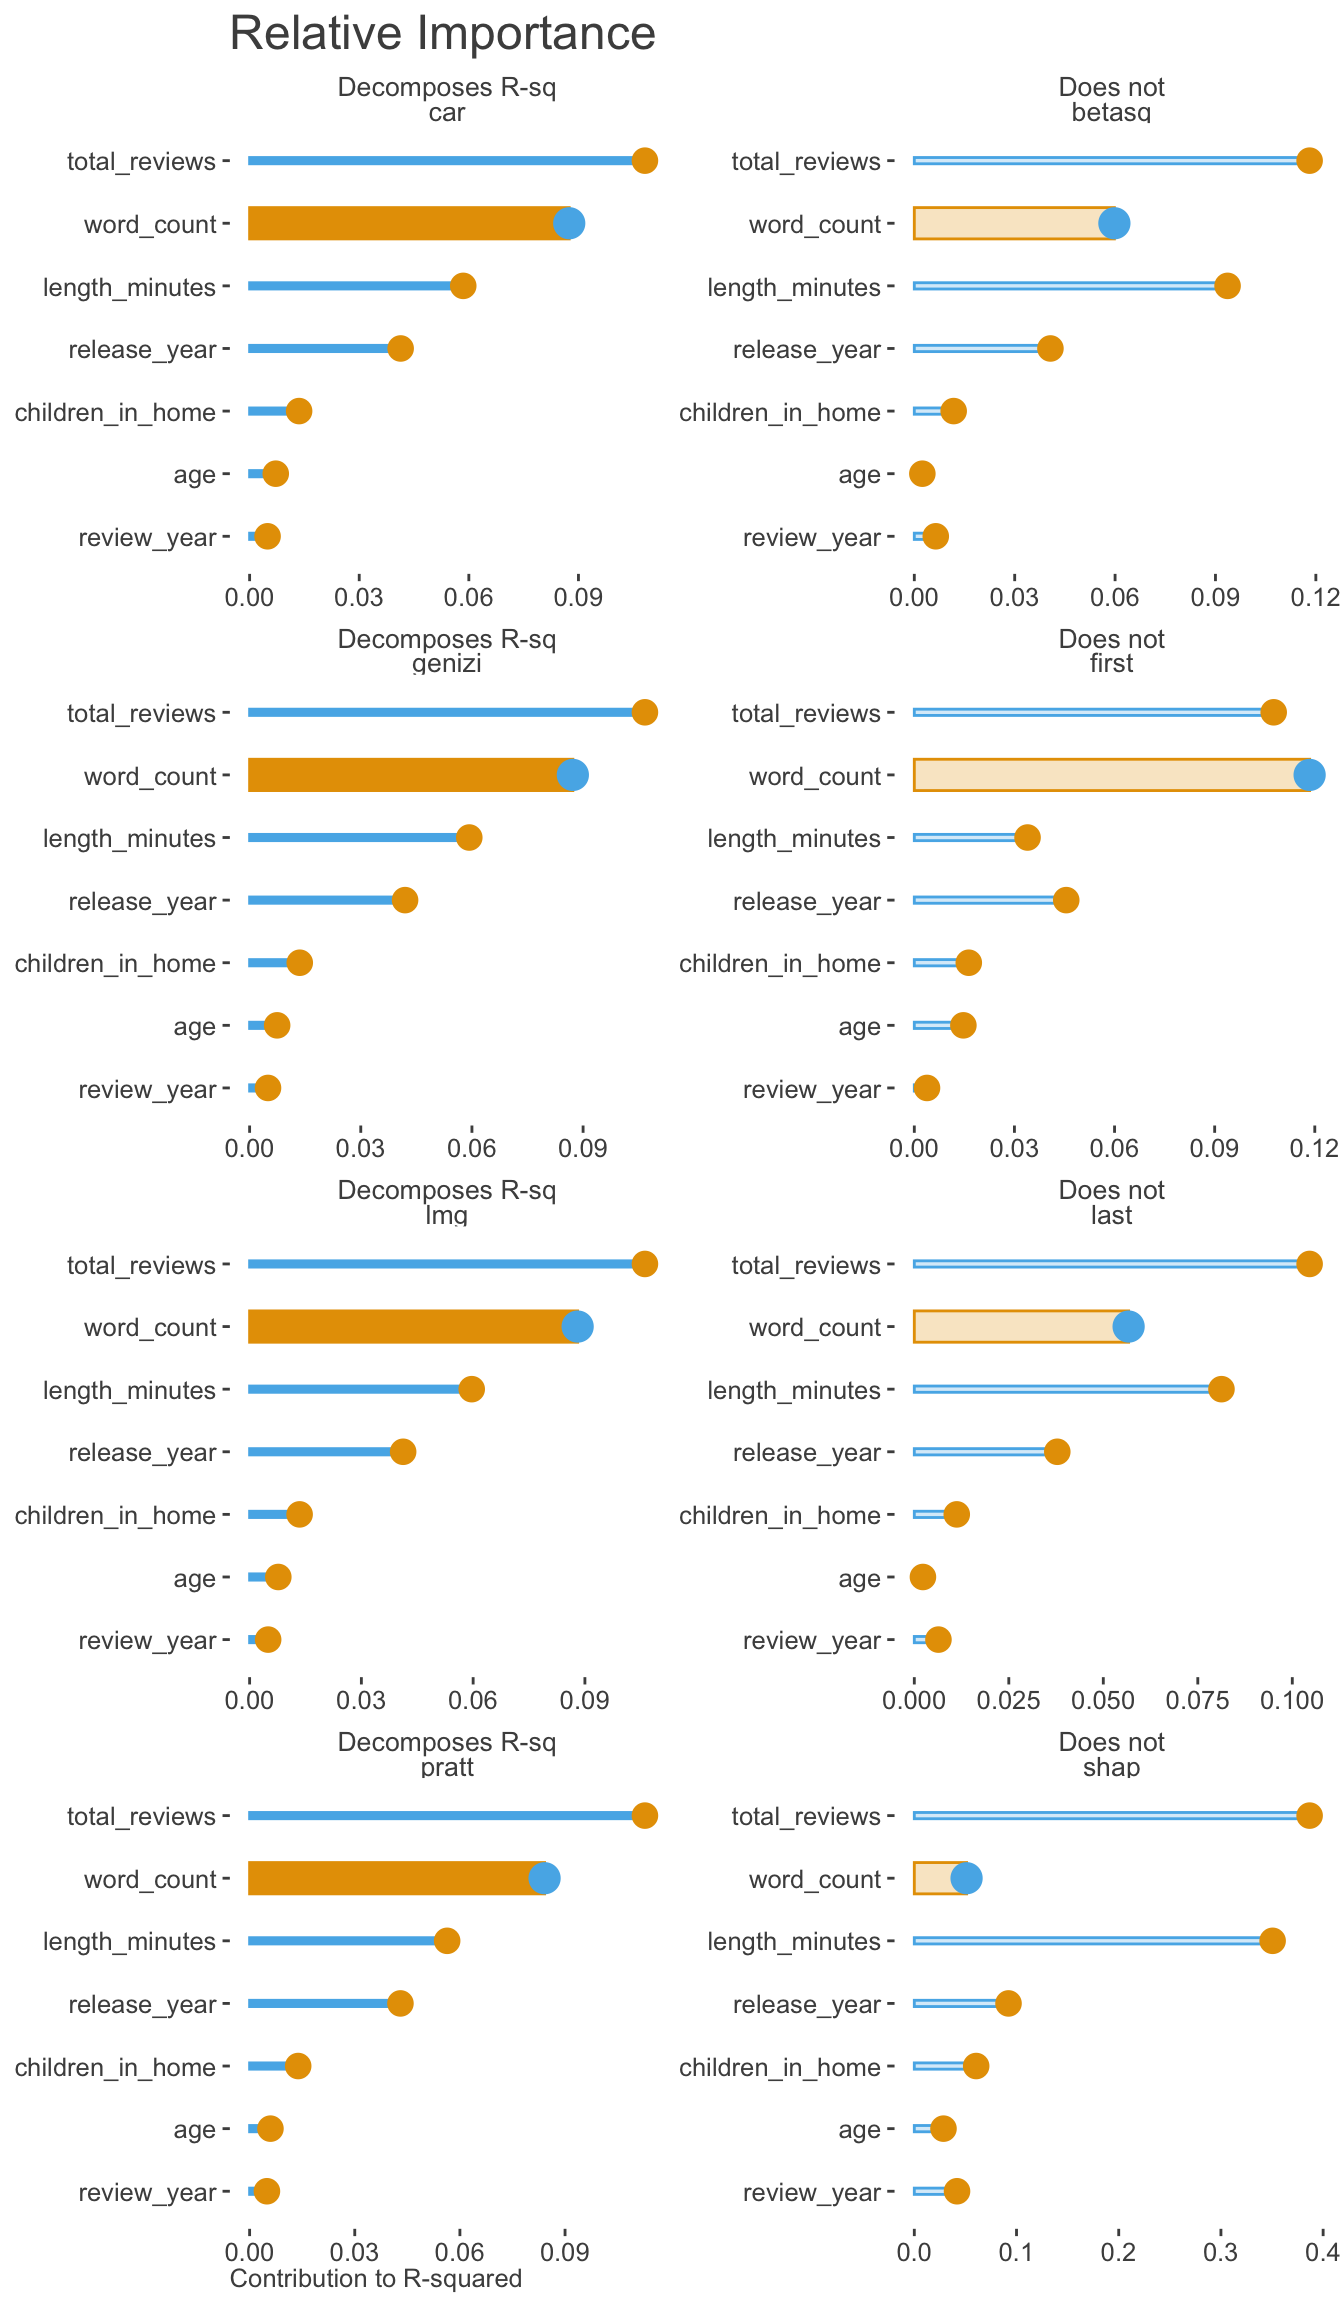
\includegraphics{linear_models_files/figure-pdf/fig-importance-1.pdf}

}

\caption{\label{fig-importance}Feature Importance by Various Methods}

\end{figure}

\subsection{Model Level
Interpretation}\label{model-level-interpretation}

As before we can move beyond feature level interpretation, but we are
still going to be concerned with the same sorts of questions - how well
does the model fit? Have we impoved the fit significantly? What do our
predictions look like, and so on.

As an example, we see that our R\textsuperscript{2} has gone up to 0.32,
but this comes with an important caveat - adding any feature would
increase our R\textsuperscript{2}, even one that was pure noise! So
while it is informative, we want to look at MSE or MAE to determine
whether the model has truly improved. In both cases they've been
reduced. For example, RMSE is now 0.52 a reduction of 12\%, so we can
feel confident that our model has improved. While there is more a lot
more to unpack, we will save doing so for the Model Criticism chapter.
At least at this point, we have an idea of how to assess our this added
complexity at the model level.

\begin{tcolorbox}[enhanced jigsaw, rightrule=.15mm, opacityback=0, left=2mm, bottomrule=.15mm, toprule=.15mm, arc=.35mm, colframe=quarto-callout-note-color-frame, leftrule=.75mm, breakable, colback=white]
\begin{minipage}[t]{5.5mm}
\textcolor{quarto-callout-note-color}{\faInfo}
\end{minipage}%
\begin{minipage}[t]{\textwidth - 5.5mm}

\textbf{Adjusted R\textsuperscript{2}}\vspace{2mm}

Part of the output contains an `adjusted' R\textsuperscript{2}. This is
a version of R\textsuperscript{2} that penalizes the addition of
features to the model as a way to account for the fact that adding
features will always increase R\textsuperscript{2}, even if they are not
useful. This is why we can't use R\textsuperscript{2} alone to determine
whether a model has improved, and why we suggest only considering it as
a descriptive statistic. But the adjusted version is kind of a hack, and
can even be negative for very poor models. If you want to compare
models, use MSE, MAE, and similar metrics.

\end{minipage}%
\end{tcolorbox}

\subsection{Other Complexity}\label{other-complexity}

\subsubsection{Categorical Features}\label{categorical-features}

Categorical features can be added to a model just like any other
feature. The main issue is that they have to be represented numerically,
because models only work on numerically coded features and targets. The
simplest and most common encoding is called a \textbf{one-hot encoding}
scheme, which creates a new feature for each category, and assigns a 1
if the observation is in that category, and a 0 otherwise. This is also
called a \textbf{dummy coding} when used for statistical models. Here is
an example of what the coding looks like for the season feature. This is
really all there is to it.

\begin{longtable*}{rlrrrr}
\toprule
rating & season & Fall & Summer & Winter & Spring \\ 
\midrule\addlinespace[2.5pt]
\textcolor[HTML]{404040}{$2.70$} & Fall & \textcolor[HTML]{404040}{$1$} & \textcolor[HTML]{404040}{$0$} & \textcolor[HTML]{404040}{$0$} & \textcolor[HTML]{404040}{$0$} \\ 
\textcolor[HTML]{404040}{$4.20$} & Fall & \textcolor[HTML]{404040}{$1$} & \textcolor[HTML]{404040}{$0$} & \textcolor[HTML]{404040}{$0$} & \textcolor[HTML]{404040}{$0$} \\ 
\textcolor[HTML]{404040}{$3.70$} & Fall & \textcolor[HTML]{404040}{$1$} & \textcolor[HTML]{404040}{$0$} & \textcolor[HTML]{404040}{$0$} & \textcolor[HTML]{404040}{$0$} \\ 
\textcolor[HTML]{404040}{$2.70$} & Fall & \textcolor[HTML]{404040}{$1$} & \textcolor[HTML]{404040}{$0$} & \textcolor[HTML]{404040}{$0$} & \textcolor[HTML]{404040}{$0$} \\ 
\textcolor[HTML]{404040}{$2.40$} & Summer & \textcolor[HTML]{404040}{$0$} & \textcolor[HTML]{404040}{$1$} & \textcolor[HTML]{404040}{$0$} & \textcolor[HTML]{404040}{$0$} \\ 
\textcolor[HTML]{404040}{$4.00$} & Summer & \textcolor[HTML]{404040}{$0$} & \textcolor[HTML]{404040}{$1$} & \textcolor[HTML]{404040}{$0$} & \textcolor[HTML]{404040}{$0$} \\ 
\textcolor[HTML]{404040}{$1.80$} & Fall & \textcolor[HTML]{404040}{$1$} & \textcolor[HTML]{404040}{$0$} & \textcolor[HTML]{404040}{$0$} & \textcolor[HTML]{404040}{$0$} \\ 
\textcolor[HTML]{404040}{$2.40$} & Summer & \textcolor[HTML]{404040}{$0$} & \textcolor[HTML]{404040}{$1$} & \textcolor[HTML]{404040}{$0$} & \textcolor[HTML]{404040}{$0$} \\ 
\textcolor[HTML]{404040}{$2.50$} & Winter & \textcolor[HTML]{404040}{$0$} & \textcolor[HTML]{404040}{$0$} & \textcolor[HTML]{404040}{$1$} & \textcolor[HTML]{404040}{$0$} \\ 
\textcolor[HTML]{404040}{$4.30$} & Summer & \textcolor[HTML]{404040}{$0$} & \textcolor[HTML]{404040}{$1$} & \textcolor[HTML]{404040}{$0$} & \textcolor[HTML]{404040}{$0$} \\ 
\bottomrule
\end{longtable*}

When using statistical models we don't have to do this ourselves. Even
other tools for machine learning models will typically have a way to
identify and appropriately handle categorical features, even in very
complex ways when it comes to deep learning models. What is important is
to be aware that they require special handling, but often this is done
behind the scenes. Now let's do a quick example using a categorical
feature with our data, and we'll keep a numeric feature as well just for
consistency.

\subsubsection{R}

\begin{Shaded}
\begin{Highlighting}[]
\NormalTok{model\_cat }\OtherTok{=} \FunctionTok{lm}\NormalTok{(}
\NormalTok{    rating }\SpecialCharTok{\textasciitilde{}}\NormalTok{ word\_count }\SpecialCharTok{+}\NormalTok{ season,}
    \AttributeTok{data =}\NormalTok{ df\_reviews}
\NormalTok{)}

\FunctionTok{summary}\NormalTok{(model\_cat)}
\end{Highlighting}
\end{Shaded}

\begin{verbatim}

Call:
lm(formula = rating ~ word_count + season, data = df_reviews)

Residuals:
    Min      1Q  Median      3Q     Max 
-1.9184 -0.3622  0.0133  0.3589  1.8372 

Coefficients:
             Estimate Std. Error t value Pr(>|t|)    
(Intercept)    3.3429     0.0530   63.11  < 2e-16 ***
word_count    -0.0394     0.0036  -10.96  < 2e-16 ***
seasonSpring  -0.0301     0.0622   -0.48     0.63    
seasonSummer   0.2743     0.0445    6.17  9.8e-10 ***
seasonWinter  -0.0700     0.0595   -1.18     0.24    
---
Signif. codes:  0 '***' 0.001 '**' 0.01 '*' 0.05 '.' 0.1 ' ' 1

Residual standard error: 0.572 on 995 degrees of freedom
Multiple R-squared:  0.176, Adjusted R-squared:  0.173 
F-statistic: 53.1 on 4 and 995 DF,  p-value: <2e-16
\end{verbatim}

\subsubsection{Python}

\begin{Shaded}
\begin{Highlighting}[]
\NormalTok{model\_cat }\OperatorTok{=}\NormalTok{ smf.ols(}
\NormalTok{    formula }\OperatorTok{=} \StringTok{"rating \textasciitilde{} word\_count + season"}\NormalTok{,}
\NormalTok{    data }\OperatorTok{=}\NormalTok{ df\_reviews}
\NormalTok{).fit()}

\NormalTok{model\_cat.summary()}
\end{Highlighting}
\end{Shaded}

\begin{verbatim}
<class 'statsmodels.iolib.summary.Summary'>
"""
                            OLS Regression Results                            
==============================================================================
Dep. Variable:                 rating   R-squared:                       0.176
Model:                            OLS   Adj. R-squared:                  0.173
Method:                 Least Squares   F-statistic:                     53.09
Date:                Sat, 02 Dec 2023   Prob (F-statistic):           1.41e-40
Time:                        12:13:44   Log-Likelihood:                -857.85
No. Observations:                1000   AIC:                             1726.
Df Residuals:                     995   BIC:                             1750.
Df Model:                           4                                         
Covariance Type:            nonrobust                                         
====================================================================================
                       coef    std err          t      P>|t|      [0.025      0.975]
------------------------------------------------------------------------------------
Intercept            3.3429      0.053     63.109      0.000       3.239       3.447
season[T.Spring]    -0.0301      0.062     -0.483      0.629      -0.152       0.092
season[T.Summer]     0.2743      0.044      6.171      0.000       0.187       0.362
season[T.Winter]    -0.0700      0.059     -1.177      0.239      -0.187       0.047
word_count          -0.0394      0.004    -10.963      0.000      -0.047      -0.032
==============================================================================
Omnibus:                        2.882   Durbin-Watson:                   2.079
Prob(Omnibus):                  0.237   Jarque-Bera (JB):                3.059
Skew:                          -0.040   Prob(JB):                        0.217
Kurtosis:                       3.259   Cond. No.                         53.5
==============================================================================

Notes:
[1] Standard Errors assume that the covariance matrix of the errors is correctly specified.
"""
\end{verbatim}

We now see the usual output. There is word count again, with its
slightly negative assocation with rating. And we have an effect for each
season as well\ldots{} except, wait a second, where is the fall effect?
The coefficients are interepreted the same way - as we move one unit on
x, we see a corresponding change in y. But moving from one category to
another requires starting at some category in the first place! So one is
chosen arbitrarily, but you would have control over this. In our model,
fall is chosen because its first alphabetically. So if we look at say,
the effect of summer, we see an increase in the rating of 0.27 relative
to fall.

A better approach to understanding categorical features for standard
linear models is through what are called \textbf{marginal effects},
which can provide a kind of average prediction for each category while
accounting for the other features in the model. Better still is to
visualize these, and we can use something like our PDP approach from
before to do so\footnote{At the time of this writing, there seems to be
  very little for this sort of thing in Python. statsmodels provides
  limited functionality, but only for logistic regression models. In R
  you have various tools like \texttt{marginaleffects},
  \texttt{emmeans}, \texttt{ggeffects} and more.}. It's actually tricky
to define `average' when there are multiple features and interactions
involved, so be careful, but we'd interpret the result similarly. In
this case, we expect higher ratings for summer releases.

\begin{figure}

{\centering 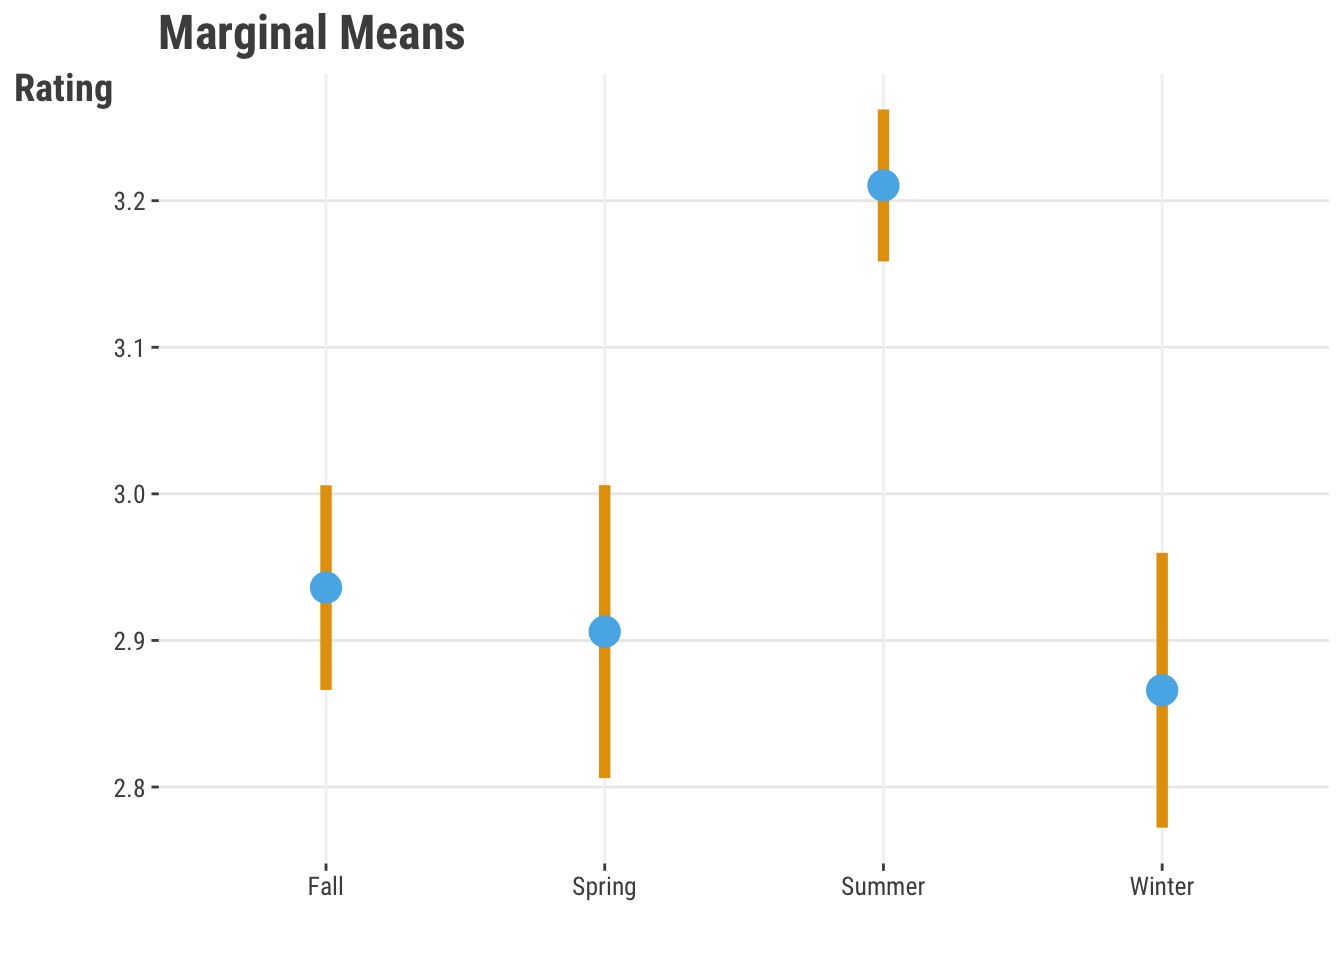
\includegraphics{linear_models_files/figure-pdf/cat-feature-viz-r-1.pdf}

}

\caption{Marginal Effects of Season on Rating}

\end{figure}

\subsubsection{Interactions (a preview)}\label{interactions-a-preview}

We'll demonstrate this more in the \hyperref[extensions]{extensions
chapter}, but a common way to add complexity in linear models is through
interactions. This is where we allow the effect of a feature to vary
depending on the values of another feature, or even itself! As a
conceptual example, we might expect that the effect of the number of
children in the home on rating is different for movies from different
genres (much higher for kids movies, maybe lower for horror movies), or
that genre and season work together in some way to affect rating
(e.g.~action movies get higher ratings in summer). We might also
consider that the length of a movie might plateau or even have a
negative effect on rating after a certain point, i.e.~having a
curvilinear effect. All of these are types of interactions we can
explore. Interactions allow us to incorporate nonlinear relationships
into the model, and so greatly extend the linear model's capabilities -
we basically get to use a linear model in a nonlinear way!

\section{Assumptions and More}\label{assumptions-and-more}

MOVE BULK OF THIS TO MODEL CRITICISM??

Every model you use has underlying assumptions which, if not met, could
potentially result in incorrect inferences. The standard linear
regression model we've shown is no different, and it has a number of
assumptions that must be met for it to be \emph{statistically} valid.
Briefly they are:

\begin{itemize}
\tightlist
\item
  That your model is not grossly misspecified (e.g., you've included the
  right features and not left out important ones)
\item
  The data your modeling reflects the population you want to make
  generalizations about
\item
  The model is linear in the parameters (i.e.~no \(\beta_1*e^\beta_2\)
  type stuff)
\item
  The features are not correlated with the error (prediction errors)
\item
  Your data observations are independent of each other
\item
  The prediction errors are homoscedastic (don't have large errors with
  certain predictions vs low with others)
\item
  Normality of the errors (i.e.~your prediction errors). Another way to
  put it is that your target variable is normally distributed
  conditional on the features.
\end{itemize}

Some of these are more important than others depending on what you're
trying to do with the model, so

Things it does not assume:

\begin{itemize}
\tightlist
\item
  That the features are normally distributed

  \begin{itemize}
  \tightlist
  \item
    For example, using categorical features is fine
  \end{itemize}
\item
  That the relationship between the features and target is linear

  \begin{itemize}
  \tightlist
  \item
    Interactions, polynomial terms, etc. are all fine
  \end{itemize}
\item
  That the features are not correlated with each other

  \begin{itemize}
  \tightlist
  \item
    They usually are
  \end{itemize}
\item
  That all linear models have these assumptions
\end{itemize}

If you don't meet these assumptions, it doesn't mean:

\begin{itemize}
\tightlist
\item
  That your model will have poor predictions
\item
  That your conclusions will necessarily be incorrect
\end{itemize}

If you do meet those assumptions, your coefficient estimates are
unbiased\footnote{This means they are correct on average, not the true
  value. And if they were biased, this is statistical bias, and has
  nothing to do with the moral or ethical implications of the data, or
  whether the features themselves are biased in measurement. Culturally
  biased data is a different problem than statistical/prediction bias or
  measurement error, though they are not mutually exclusive. The latter
  can more readily be tested, while the former is usually more difficult
  to assess. If our moview reviews only came from a website with a
  paywall, they would be biased if we wanted to use them to refer to
  general public opinion. Our model results are unaffected by this
  scenario, as long as they are used to generalize only to that
  population of people who pay for the website. If we wanted to
  generalize to the general public, we would need to account for this
  bias in some way, or use a different data source. MOVE THIS TO SOME
  OTHER CHAPTER (DATA?)}, and in general, your statistical inferences
are correct ones. If you don't meet them, there are alternative versions
of the linear model you could use that would get around the problem. For
example, data that runs over a sequence of time (\textbf{time series}
data) violates the independence assumption, but we would use a
\textbf{time series} or similar model instead. If normality is difficult
to meet, you could assume a different data generating distribution.
We'll discuss some of these in the \hyperref[extensions]{extensions
chapter}, but it's also important to note that not meeting the
assumptions may only mean you'll prefer a different type of linear or
other model to use for the data. Our opinion is that not meeting the
assumptions often is the result of a poor model, e.g.~using poor
features in an \textbf{underspecified} way (e.g.~not including
interactions).

On top of not meeting the assumptions, we may in fact introduce bias to
get better prediction! For example, we might use a \textbf{penalized
regression} model to reduce the variance in our predictions, at the cost
of introducing bias in the coefficients. We'll talk more of this in the
\hyperref[machine-learning]{machine learning} chapter, but suffice it to
say for now, if you are more interested in prediction, you may be less
interested in the statistical assumptions of the basic linear model.

\subsection{More Complex Models}\label{more-complex-models}

Let's say your running some XGBoost or Deep Linear Model X and getting
outsanding predictions. Assumption smumptions you say! And you might
even be right! But if you want to talk confidently about feature
contributions, or know something about the uncertainty in the
predictions (which you're assessing right?) well, maybe you might want
to know if you're meeting your assumptions. Some of them are:

\begin{itemize}
\tightlist
\item
  You have enough data to make the model generalizable
\item
  Your data isn't biased (e.g., you don't have 90\% of your data from
  one region when you want to talk about a whole area)
\item
  You adequately sampled the hyperparameter space (e.g.~you didn't just
  use the defaults or a small grid search)
\item
  Your observations are independent or at least \textbf{exchangeable}
  and don't have \textbf{data leakage}, or you are explicitly modeling
  spatio-temporal dependence
\item
  That all the parameter settings you set are correct or at least viable
  (e.g.~you let the model run for a long enough set of iterations, your
  batch size was adequate, you had enough hidden layers, etc.)
\end{itemize}

And if you want to talk about specific feature contributions:

\begin{itemize}
\tightlist
\item
  The features are largely uncorrelated
\item
  The features largely do not interact (but then why are you doing a
  complex model that is inherently interactive), or that your
  understanding of feature contribution deals with the interactions
\end{itemize}

Yeah\ldots{} so, sorry to say, using non-statistical models doesn't mean
you don't have to worry about assumptions, you still have some of the
old stuff and some new ones to boot.

Model criticism and diagnostics, but briefly note something here.

\section{Classification}\label{classification}

We've been using a continuous target, but what about a categorical
target? For example, what if we just had a binary target of whether a
movie was good or bad? We will dive much more into classification models
in our upcoming chapters, but it turns out that we can still formulate
it as a linear model problem. The main difference is that we use a
transformation of our linear combination, sometimes called a
\textbf{link function}, and we'll need to use a different
\textbf{objective function} rather than least squares, such as the
binomial likelihood, to deal with the binary target. This also means
we'll move away from R\textsuperscript{2} as a measure of model fit, and
look at something something else, like accuracy.

Graphically we can see it in the following way, which when compared with
our linear model, doesn't look much different. In what follows, we
create our linear combination \(\mu\) and put it through the sigmoid
function \(\sigma\), which is a common link function for binary
targets\footnote{The sigmoid function in this case is the inverse
  logistic function, and the resulting statistical model is called
  logistic regression. In other contexts the model would not be a
  logistic regression, but this is still a very commmonly used
  \emph{activation function}. But many others could potentially be used
  e.g.~using a normal instead of logistic distribution, resulting in the
  so-called probit model.}. The result is a probability, which we can
then use to classify the observation as good or bad based on a chosen
threshold. We'll see this in more detail in the classification chapter.

\begin{figure}[H]

{\centering \includegraphics[width=3.18in,height=2.17in]{linear_models_files/figure-latex/mermaid-figure-2.png}

}

\end{figure}

Linear Model with Transformation

As soon as we move away from the standard linear model and use
transformations of our linear predictor, simple coefficient
interpretation becomes difficult, sometimes exceedingly so. What will
help

\section{More linear models}\label{more-linear-models}

Before we leave our humble linear model, let's look at some others

Generalize Linear Models and related

\begin{itemize}
\tightlist
\item
  True GLM e.g.~logistic, poisson
\item
  Other distributions: beta regression, tweedie, t (so-called robust),
  truncated
\item
  Penalized regression: ridge, lasso, elastic net
\item
  Censored outcomes: Survival models, tobit
\end{itemize}

Multivariate/multiclass/multipart

\begin{itemize}
\tightlist
\item
  Multivariate regression (multiple targets)
\item
  Multinomial/Categorical/Ordinal regression (\textgreater2 classes)
\item
  Zero (or some number) -inflated/hurdle/altered
\item
  Mixture models and Cluster analysis
\end{itemize}

Random Effects

\begin{itemize}
\tightlist
\item
  Mixed effects models (random intercepts/coefficients)
\item
  Generalized additive models (GAMMs)
\item
  Spatial models (CAR)
\item
  Time series models (ARIMA)
\item
  Factor analysis
\end{itemize}

Latent Linear Models

\begin{itemize}
\tightlist
\item
  PCA, Factor Analysis
\item
  Mixture models
\item
  Structural Equation Modeling, Graphical models generally
\end{itemize}

All of these are explicitly linear models or can be framed as such, and
most are either identical in description to what you've already seen or
require only a tweak or two - e.g.~a different distribution, a different
link function, penalizing the coefficients, etc. In other cases, we can
bounce from one to the another. For example we can reshape our
multivariate outcome to be amenable to a mixed model approach, and get
the exact same results. We can potentially add a random effect to any
model, and that random effect can be based on time, spatial or other
considerations. The important thing to know is that the linear model is
a very flexible tool, and allows you to model most of the types of
outcomes were interested in. As such, it's a very powerful tool.

What about nonlinear models?

\section{Commentary}\label{commentary-1}

Linear models are a very popular tool for data analysis, and for good
reason. They are relatively easy to understand, and they are very
flexible. They can be used for prediction, explanation, and inference,
and they can be used for a wide variety of data types. They are also
very easy to interpret, and there are many tools at our disposal to help
us understand them. But they are not without their limitations, and
we'll discuss some of those here.

\begin{itemize}
\tightlist
\item
  Opinions
\item
  Limitations/Failure points
\item
  Summary
\end{itemize}

\subsection{Choose your own
adventure}\label{choose-your-own-adventure-1}

Now that you've got the basics, where do you want to go?

\begin{itemize}
\tightlist
\item
  If you want a deeper dive into how we get the results from our model:
  head \hyperref[estimation]{Estimation}
\item
  If you want to know more about how to understand the model: head to
  \hyperref[model-criticism]{Model Criticism}
\item
  If you want to do some more modeling: go to
  \hyperref[extensions]{Extensions} or
  \hyperref[machine-learning]{Machine Learning}
\item
  Got more data questions? Go to the \hyperref[data]{Data chapter}
\end{itemize}

\section{Quick Exercise}\label{quick-exercise}

\begin{itemize}
\tightlist
\item
  Import X Data. Stick with the current data if you want, just try out
  other features, or maybe try the world happiness data 2018 data . You
  can find details about it in the appendix ADD LINK.
\item
  Fit a linear model, try to keep it to no more than three features.
\item
  Get all the predictions for the data, and try at least
\item
  Interpret the coefficients
\item
  Assess the model fit
\end{itemize}

\# refs to add

Statistical modeling rigorous: Econometrics books like Wooldrigde,
Greene, etc.

Basic DS?

Assumptions: https://statmodeling.stat.columbia.edu/2013/08/04/19470/

\chapter{Knowing Your Model}\label{knowing-your-model}

In addition to giving the world one of the greatest television show
theme songs -- Quincy Jones' \emph{The Streetbeater} -- \emph{Sanford \&
Son} gave us an insightful quote for offering criticism: ``You big
dummy.'' While we don't advocate for swearing at or denigrating your
model, wow do you know if your model is performing up to your
expectations? It is easy to look at your coefficients, \emph{t}-values,
and an adjusted \(R^2\), and say, ``Wow! Look at this great model!''
Your friends will be envious of such terrific \emph{p}-values and all of
the strangers that you tell at social functions will be impressed. What
happens if that model falls apart on new data, though? What if a
stakeholder wants to know exactly how a prediction was made for a
specific business decision? All of the stars that you gleefully pointed
towards in your console will not offer you any real answers.

Instead of falling in immediate love with your model, you should ask
real questions of it. How does it perform on different slices of data?
Do predictions make sense? Is your classification cut-point appropriate?
In other words, you should criticize your model before you decide it can
be used for its intended purposes. Remember that it is \textbf{data
modeling}, not \textbf{data truthing}. In other words, you should always
be prepared to call your model a ``big dummy''.

\section{Model Metrics}\label{model-metrics-1}

Regression and classification have very different metrics for assessing
model performance. We want to give you a sample of some of the more
common one, but we also want to acknowledge that there are many more
that you can use! We would always recommend looking at a few different
metrics to get a better sense of how your model is performing.

\subsection{Regression Metrics}\label{regression-metrics}

Recall that a primary goal of our standard linear model is to produce
\(\hat{y}\) -- the predicted outcome. Since we are predicting a value,
we need to be able to compare that prediction to its actual value. The
closer our prediction is to the actual value, the better our model is
performing.

Before we create a model, we are going to read in our data and then
create two different splits within our data: a \textbf{training} set and
a \textbf{testing} set. In other words, we are going to
\textbf{partition} our data so that we can train a model and then see
how well that model does with new data.

This basic split is the foundation of \textbf{cross-validation}.
Cross-validation is a method for partitioning data into training and
testing sets, but it does so in a way that allows you to train and test
your model multiple times. We will not be covering cross-validation in
this book, but we would strongly encourage you to learn more about it.

\subsubsection{R}

\begin{Shaded}
\begin{Highlighting}[]
\NormalTok{reviews }\OtherTok{\textless{}{-}} \FunctionTok{read.csv}\NormalTok{(}
  \StringTok{"data/movie\_reviews\_processed.csv"}
\NormalTok{)}

\NormalTok{initial\_split }\OtherTok{\textless{}{-}} \FunctionTok{sample}\NormalTok{(}
  \AttributeTok{x =} \DecValTok{1}\SpecialCharTok{:}\FunctionTok{nrow}\NormalTok{(reviews), }
  \AttributeTok{size =} \FunctionTok{nrow}\NormalTok{(reviews) }\SpecialCharTok{*}\NormalTok{ .}\DecValTok{75}\NormalTok{, }
  \AttributeTok{replace =} \ConstantTok{FALSE}
\NormalTok{)}

\NormalTok{training\_data }\OtherTok{\textless{}{-}}\NormalTok{ reviews[initial\_split, ]}

\NormalTok{testing\_data }\OtherTok{\textless{}{-}}\NormalTok{ reviews[}\SpecialCharTok{{-}}\NormalTok{initial\_split, ]}
\end{Highlighting}
\end{Shaded}

\subsubsection{Python}

\begin{Shaded}
\begin{Highlighting}[]
\ImportTok{import}\NormalTok{ pandas }\ImportTok{as}\NormalTok{ pd}
\ImportTok{import}\NormalTok{ numpy }\ImportTok{as}\NormalTok{ np}

\NormalTok{reviews }\OperatorTok{=}\NormalTok{ pd.read\_csv(}\StringTok{"data/movie\_reviews\_processed.csv"}\NormalTok{)}

\NormalTok{initial\_split }\OperatorTok{=}\NormalTok{ np.random.choice(}
\NormalTok{    reviews.index, }
\NormalTok{    size }\OperatorTok{=} \BuiltInTok{int}\NormalTok{(reviews.shape[}\DecValTok{0}\NormalTok{] }\OperatorTok{*} \FloatTok{.75}\NormalTok{), }
\NormalTok{    replace }\OperatorTok{=} \VariableTok{False}
\NormalTok{)}

\NormalTok{training\_data }\OperatorTok{=}\NormalTok{ reviews.iloc[initial\_split, :]}

\NormalTok{testing\_data }\OperatorTok{=}\NormalTok{ reviews.iloc[}\OperatorTok{{-}}\NormalTok{initial\_split, :]}
\end{Highlighting}
\end{Shaded}

You'll notice that we created training data with 75\% of our data and we
will use the other 25\% to test our model. With training data in hand,
let's produce a model to predict rating

\subsubsection{R}

\begin{Shaded}
\begin{Highlighting}[]
\NormalTok{model\_train }\OtherTok{\textless{}{-}} \FunctionTok{lm}\NormalTok{(}
\NormalTok{  rating }\SpecialCharTok{\textasciitilde{}} 
\NormalTok{    review\_year\_0 }\SpecialCharTok{+}\NormalTok{ release\_year\_0 }\SpecialCharTok{+} 
\NormalTok{    age\_sc }\SpecialCharTok{+}\NormalTok{ length\_minutes\_sc }\SpecialCharTok{+} 
\NormalTok{    total\_reviews\_sc }\SpecialCharTok{+}\NormalTok{ word\_count\_sc }\SpecialCharTok{+}
\NormalTok{    genre }\SpecialCharTok{+}\NormalTok{ gender }\SpecialCharTok{+}
\NormalTok{    reviewer\_type }\SpecialCharTok{+}\NormalTok{ work\_status }\SpecialCharTok{+}
\NormalTok{    season, }
\NormalTok{  training\_data}
\NormalTok{)}
\end{Highlighting}
\end{Shaded}

\subsubsection{Python}

\begin{Shaded}
\begin{Highlighting}[]
\ImportTok{import}\NormalTok{ statsmodels.api }\ImportTok{as}\NormalTok{ sm}

\NormalTok{features }\OperatorTok{=}\NormalTok{ [}\StringTok{"review\_year\_0"}\NormalTok{, }\StringTok{"release\_year\_0"}\NormalTok{,}
  \StringTok{"age\_sc"}\NormalTok{, }\StringTok{"length\_minutes\_sc"}\NormalTok{, }
  \StringTok{"total\_reviews\_sc"}\NormalTok{, }\StringTok{"word\_count\_sc"}\NormalTok{, }
  \StringTok{"genre"}\NormalTok{, }\StringTok{"gender"}\NormalTok{, }
  \StringTok{"reviewer\_type"}\NormalTok{, }\StringTok{"work\_status"}\NormalTok{, }
  \StringTok{"season"}\NormalTok{]}

\NormalTok{X\_features }\OperatorTok{=}\NormalTok{ training\_data[features]}
\NormalTok{X\_features }\OperatorTok{=}\NormalTok{ sm.add\_constant(X\_features)}
\NormalTok{X\_features }\OperatorTok{=}\NormalTok{ pd.get\_dummies(X\_features)}
\NormalTok{X\_features }\OperatorTok{=}\NormalTok{ X\_features.drop(}
\NormalTok{  columns}\OperatorTok{=}\NormalTok{[}\StringTok{"work\_status\_Unemployed"}\NormalTok{, }\StringTok{"season\_Winter"}\NormalTok{]}
\NormalTok{  )}
\NormalTok{X\_features }\OperatorTok{=}\NormalTok{ X\_features.values.astype(}\BuiltInTok{float}\NormalTok{)}
\NormalTok{y\_target }\OperatorTok{=}\NormalTok{ training\_data[}\StringTok{"rating"}\NormalTok{].values.astype(}\BuiltInTok{float}\NormalTok{)}

\NormalTok{model\_train }\OperatorTok{=}\NormalTok{ sm.OLS(y\_target, X\_features).fit()}
\end{Highlighting}
\end{Shaded}

Now that we have a model on our training data, we can use it to make
predictions on our test data:

\subsubsection{R}

\begin{Shaded}
\begin{Highlighting}[]
\NormalTok{predictions }\OtherTok{\textless{}{-}} \FunctionTok{predict}\NormalTok{(model\_train, }\AttributeTok{newdata =}\NormalTok{ testing\_data)}
\end{Highlighting}
\end{Shaded}

\subsubsection{Python}

\begin{Shaded}
\begin{Highlighting}[]
\NormalTok{X\_features\_testing }\OperatorTok{=}\NormalTok{ testing\_data[features]}
\NormalTok{X\_features\_testing }\OperatorTok{=}\NormalTok{ sm.add\_constant(X\_features\_testing)}
\NormalTok{X\_features\_testing }\OperatorTok{=}\NormalTok{ pd.get\_dummies(X\_features\_testing)}
\NormalTok{X\_features\_testing }\OperatorTok{=}\NormalTok{ X\_features\_testing.drop(}
\NormalTok{  columns}\OperatorTok{=}\NormalTok{[}\StringTok{"work\_status\_Unemployed"}\NormalTok{, }\StringTok{"season\_Winter"}\NormalTok{]}
\NormalTok{  )}
\NormalTok{X\_features\_testing }\OperatorTok{=}\NormalTok{ X\_features\_testing.values.astype(}\BuiltInTok{float}\NormalTok{)}
\NormalTok{y\_target\_testing }\OperatorTok{=}\NormalTok{ testing\_data[}\StringTok{"rating"}\NormalTok{].values.astype(}\BuiltInTok{float}\NormalTok{)}

\NormalTok{predictions }\OperatorTok{=}\NormalTok{ model\_train.predict(X\_features\_testing)}
\end{Highlighting}
\end{Shaded}

The goal now is to find out how close our predictions match reality.
Let's look at them first:

\includegraphics{model_criticism_files/figure-pdf/unnamed-chunk-8-1.pdf}

Obviously, our points for do not make a perfect line. Therefore, we need
to determine how far off we are. There are a number of metrics that can
be used to measure this. We'll go through a few of them here.

\subsubsection{Mean Squared Error}\label{mean-squared-error}

One of the most common metrics is the mean squared error (MSE). The MSE
is the average of the squared differences between the predicted and
actual values. It is calculated as follows:

\[MSE = \frac{1}{n}\sum_{i=1}^{n}(y_i - \hat{y}_i)^2\]

MSE is a great metric for penalizing large errors. Since errors are
squared, the larger the error, the larger the penalty.

\subsubsection{R}

\begin{Shaded}
\begin{Highlighting}[]
\FunctionTok{mean}\NormalTok{((testing\_data}\SpecialCharTok{$}\NormalTok{rating }\SpecialCharTok{{-}}\NormalTok{ predictions)}\SpecialCharTok{\^{}}\DecValTok{2}\NormalTok{)}
\end{Highlighting}
\end{Shaded}

\begin{verbatim}
[1] 0.1041212
\end{verbatim}

\begin{Shaded}
\begin{Highlighting}[]
\NormalTok{Metrics}\SpecialCharTok{::}\FunctionTok{mse}\NormalTok{(testing\_data}\SpecialCharTok{$}\NormalTok{rating, predictions)}
\end{Highlighting}
\end{Shaded}

\begin{verbatim}
[1] 0.1041212
\end{verbatim}

\subsubsection{Python}

\begin{Shaded}
\begin{Highlighting}[]
\ImportTok{from}\NormalTok{ sklearn.metrics }\ImportTok{import}\NormalTok{ mean\_squared\_error}

\NormalTok{np.mean((testing\_data.rating }\OperatorTok{{-}}\NormalTok{ predictions)}\OperatorTok{**}\DecValTok{2}\NormalTok{)}
\end{Highlighting}
\end{Shaded}

\begin{verbatim}
0.11016692840509355
\end{verbatim}

\begin{Shaded}
\begin{Highlighting}[]
\NormalTok{mean\_squared\_error(testing\_data.rating, predictions)}
\end{Highlighting}
\end{Shaded}

\begin{verbatim}
0.11016692840509355
\end{verbatim}

\subsubsection{Mean Absolute Error}\label{mean-absolute-error}

The mean absolute error (MAE) is the average of the absolute differences
between the predicted and actual values. It is calculated as follows:

\[MAE = \frac{1}{n}\sum_{i=1}^{n}|y_i - \hat{y}_i|\]

MAE is a great metric when all you really want to know is how far off
your predictions are from the actual values. It is not as sensitive to
large errors as the MSE.

\subsubsection{R}

\begin{Shaded}
\begin{Highlighting}[]
\FunctionTok{mean}\NormalTok{(}\FunctionTok{abs}\NormalTok{(testing\_data}\SpecialCharTok{$}\NormalTok{rating }\SpecialCharTok{{-}}\NormalTok{ predictions))}
\end{Highlighting}
\end{Shaded}

\begin{verbatim}
[1] 0.2559888
\end{verbatim}

\begin{Shaded}
\begin{Highlighting}[]
\NormalTok{Metrics}\SpecialCharTok{::}\FunctionTok{mae}\NormalTok{(testing\_data}\SpecialCharTok{$}\NormalTok{rating, predictions)}
\end{Highlighting}
\end{Shaded}

\begin{verbatim}
[1] 0.2559888
\end{verbatim}

\subsubsection{Python}

\begin{Shaded}
\begin{Highlighting}[]
\ImportTok{from}\NormalTok{ sklearn.metrics }\ImportTok{import}\NormalTok{ mean\_absolute\_error}

\NormalTok{np.mean(}\BuiltInTok{abs}\NormalTok{(testing\_data.rating }\OperatorTok{{-}}\NormalTok{ predictions))}
\end{Highlighting}
\end{Shaded}

\begin{verbatim}
0.26368605870245754
\end{verbatim}

\begin{Shaded}
\begin{Highlighting}[]
\NormalTok{mean\_absolute\_error(testing\_data.rating, predictions)}
\end{Highlighting}
\end{Shaded}

\begin{verbatim}
0.26368605870245754
\end{verbatim}

\subsubsection{Root Mean Squared Error}\label{root-mean-squared-error}

Perhaps the regression metric that you are most likely to encounter in
the wild, the root mean squared error (RMSE) is the square root of the
average of the squared differences between the predicted and actual
values. It is calculated as follows:

\[RMSE = \sqrt{\frac{1}{n}\sum_{i=1}^{n}(y_i - \hat{y}_i)^2}\]

\subsubsection{R}

\begin{Shaded}
\begin{Highlighting}[]
\FunctionTok{sqrt}\NormalTok{(}\FunctionTok{mean}\NormalTok{((testing\_data}\SpecialCharTok{$}\NormalTok{rating }\SpecialCharTok{{-}}\NormalTok{ predictions)}\SpecialCharTok{\^{}}\DecValTok{2}\NormalTok{))}
\end{Highlighting}
\end{Shaded}

\begin{verbatim}
[1] 0.3226782
\end{verbatim}

\begin{Shaded}
\begin{Highlighting}[]
\NormalTok{Metrics}\SpecialCharTok{::}\FunctionTok{rmse}\NormalTok{(testing\_data}\SpecialCharTok{$}\NormalTok{rating, predictions)}
\end{Highlighting}
\end{Shaded}

\begin{verbatim}
[1] 0.3226782
\end{verbatim}

\subsubsection{Python}

\begin{Shaded}
\begin{Highlighting}[]
\ImportTok{from}\NormalTok{ sklearn.metrics }\ImportTok{import}\NormalTok{ mean\_squared\_error}

\NormalTok{np.sqrt(np.mean((testing\_data.rating }\OperatorTok{{-}}\NormalTok{ predictions)}\OperatorTok{**}\DecValTok{2}\NormalTok{))}
\end{Highlighting}
\end{Shaded}

\begin{verbatim}
0.3319140376740543
\end{verbatim}

\begin{Shaded}
\begin{Highlighting}[]
\NormalTok{np.sqrt(mean\_squared\_error(testing\_data.rating, predictions))}
\end{Highlighting}
\end{Shaded}

\begin{verbatim}
0.3319140376740543
\end{verbatim}

\subsubsection{Mean Absolute Percentage
Error}\label{mean-absolute-percentage-error}

The mean absolute percentage error (MAPE) is the average of the absolute
differences between the predicted and actual values, expressed as a
percentage of the actual values. It is calculated as follows:

\[MAPE = \frac{1}{n}\sum_{i=1}^{n}\frac{|y_i - \hat{y}_i|}{y_i}\]

\subsubsection{R}

\begin{Shaded}
\begin{Highlighting}[]
\FunctionTok{mean}\NormalTok{(}
  \FunctionTok{abs}\NormalTok{(testing\_data}\SpecialCharTok{$}\NormalTok{rating }\SpecialCharTok{{-}}\NormalTok{ predictions) }\SpecialCharTok{/} 
\NormalTok{    testing\_data}\SpecialCharTok{$}\NormalTok{rating}
\NormalTok{)}
\end{Highlighting}
\end{Shaded}

\begin{verbatim}
[1] 0.08830737
\end{verbatim}

\begin{Shaded}
\begin{Highlighting}[]
\NormalTok{Metrics}\SpecialCharTok{::}\FunctionTok{mape}\NormalTok{(testing\_data}\SpecialCharTok{$}\NormalTok{rating, predictions)}
\end{Highlighting}
\end{Shaded}

\begin{verbatim}
[1] 0.08830737
\end{verbatim}

\subsubsection{Python}

\begin{Shaded}
\begin{Highlighting}[]
\ImportTok{from}\NormalTok{ sklearn.metrics }\ImportTok{import}\NormalTok{ mean\_absolute\_percentage\_error}

\NormalTok{np.mean(}
    \BuiltInTok{abs}\NormalTok{(testing\_data.rating }\OperatorTok{{-}}\NormalTok{ predictions) }\OperatorTok{/} 
\NormalTok{    testing\_data.rating}
\NormalTok{)}
\end{Highlighting}
\end{Shaded}

\begin{verbatim}
0.0918768841406381
\end{verbatim}

\begin{Shaded}
\begin{Highlighting}[]
\NormalTok{mean\_absolute\_percentage\_error(testing\_data.rating, predictions)}
\end{Highlighting}
\end{Shaded}

\begin{verbatim}
0.0918768841406381
\end{verbatim}

\subsubsection{Which To Use?}\label{which-to-use}

In the end, it won't hurt to look at a few of these metrics to get a
better idea of how well your model is performing. You will
\textbf{always} be using these metrics to compare different models, so
use a few of them to get a better sense of how well your models are
performing relative to one another. Does adding a variable help drive
down RMSE, indicating that the variable helps to reduce large errors? In
other words, does adding complexity to your model provide a big
reduction in error? If adding variables doesn't help reduce error, do
you really need to include it in your modelU+0203D;

\subsection{Classification Metrics}\label{classification-metrics}

Whenever we are classifying outcomes, we don't have the same ability to
compare a predicted score to an observed score -- instead, we are going
to use the predicted probability of an outcome, establish a cut-point
for that probability, convert everything below that cut-point to 0, and
then convert everything at or above that cut-point to 1. We can then
compare a table predicted and actual \textbf{classes}.

Let's start with a model to predict whether a review is ``good'' or
``bad''. We will use the same training and testing data that we created
above.

\subsubsection{R}

\begin{Shaded}
\begin{Highlighting}[]
\NormalTok{logistic\_model\_train }\OtherTok{\textless{}{-}} \FunctionTok{glm}\NormalTok{(}
\NormalTok{  rating\_good }\SpecialCharTok{\textasciitilde{}} 
\NormalTok{    review\_year\_0 }\SpecialCharTok{+}\NormalTok{ release\_year\_0 }\SpecialCharTok{+} 
\NormalTok{    age\_sc }\SpecialCharTok{+}\NormalTok{ length\_minutes\_sc }\SpecialCharTok{+} 
\NormalTok{    total\_reviews\_sc }\SpecialCharTok{+}\NormalTok{ word\_count\_sc }\SpecialCharTok{+}
\NormalTok{    genre }\SpecialCharTok{+}\NormalTok{ gender }\SpecialCharTok{+}
\NormalTok{    reviewer\_type }\SpecialCharTok{+}\NormalTok{ work\_status }\SpecialCharTok{+}
\NormalTok{    season, }
\NormalTok{  training\_data, }
  \AttributeTok{family =}\NormalTok{ binomial}
\NormalTok{)}
\end{Highlighting}
\end{Shaded}

\subsubsection{Python}

\begin{Shaded}
\begin{Highlighting}[]
\ImportTok{import}\NormalTok{ statsmodels.api }\ImportTok{as}\NormalTok{ sm}
\ImportTok{from}\NormalTok{ statsmodels.genmod.families }\ImportTok{import}\NormalTok{ Binomial}

\NormalTok{logistic\_model\_train }\OperatorTok{=}\NormalTok{ sm.GLM(}
\NormalTok{    training\_data.rating\_good,}
\NormalTok{    X\_features,}
\NormalTok{    family }\OperatorTok{=}\NormalTok{ Binomial()}
\NormalTok{).fit()}
\end{Highlighting}
\end{Shaded}

Now that we have our model trained, we can use it to get the predicted
probabilities for each observation.

\subsubsection{R}

\begin{Shaded}
\begin{Highlighting}[]
\NormalTok{predictions }\OtherTok{\textless{}{-}} \FunctionTok{predict}\NormalTok{(logistic\_model\_train, }
                       \AttributeTok{newdata =}\NormalTok{ testing\_data, }
                       \AttributeTok{type =} \StringTok{"response"}\NormalTok{)}
\end{Highlighting}
\end{Shaded}

\subsubsection{Python}

\begin{Shaded}
\begin{Highlighting}[]
\NormalTok{predictions }\OperatorTok{=}\NormalTok{ logistic\_model\_train.predict(X\_features\_testing)}
\end{Highlighting}
\end{Shaded}

We are going to take those probability values and make a decision to
convert everything above .49 to the positive class (a ``good'' review).
It is a bold assumption, but one that we will make at first!

\subsubsection{R}

\begin{Shaded}
\begin{Highlighting}[]
\NormalTok{predictions }\OtherTok{\textless{}{-}} \FunctionTok{ifelse}\NormalTok{(predictions }\SpecialCharTok{\textgreater{}}\NormalTok{ .}\DecValTok{49}\NormalTok{ , }\DecValTok{1}\NormalTok{, }\DecValTok{0}\NormalTok{)}
\end{Highlighting}
\end{Shaded}

\subsubsection{Python}

\begin{Shaded}
\begin{Highlighting}[]
\NormalTok{predictions }\OperatorTok{=}\NormalTok{ np.where(predictions }\OperatorTok{\textgreater{}} \FloatTok{.49}\NormalTok{, }\DecValTok{1}\NormalTok{, }\DecValTok{0}\NormalTok{)}

\NormalTok{predictions }\OperatorTok{=}\NormalTok{ pd.Series(predictions)}
\end{Highlighting}
\end{Shaded}

\subsubsection{Confusion Matrix}\label{confusion-matrix}

The confusion matrix is a table that shows the number of correct and
incorrect predictions made by the model.

Let's give some names to each element in that table, so that we have a
little more clarity about what they signify:

\begin{verbatim}
      0      1
0 TN:80  FN:15
1 FP:29 TP:126
\end{verbatim}

\begin{itemize}
\item
  \textbf{TN}: A True Negative is an outcome where the model correctly
  predicts the negative class -- the model correctly predicted that the
  review was not good.
\item
  \textbf{FN}: A False Negative is an outcome where the model
  incorrectly predicts the negative class -- the model incorrectly
  predicted that the review was not good.
\item
  \textbf{FP}: A False Positive is an outcome where the model
  incorrectly predicts the positive class -- the model incorrectly
  predicted that the review was good.
\item
  \textbf{TP}: A True Positive is an outcome where the model correctly
  predicts the positive class -- the model correctly predicted that the
  review was good.
\end{itemize}

In an ideal world, we would have all of our observations fitting nicely
in the diagonal of that table. Unfortunately, we don't live in the ideal
world and we always have values in the off diagonal. The more values we
have in the off diagonal (i.e., in the FN and FP spots), the worse our
model is at classifying outcomes.

Let's look at some metrics that will help to see if we've got a suitable
model or not.

\subsubsection{Accuracy}\label{accuracy}

Accuracy is the first thing you see and the last thing that you trust!
Of all the metrics to assess the quality of classification, accuracy is
the easiest to cheat. If you have any \textbf{class imbalance} (i.e.,
one class within the target has far more observations than the other),
you can get a high accuracy by simply predicting the majority class all
of the time.

Accuracy's allure is in its simplicity. The accuracy is the proportion
of correct predictions made by the model. It is calculated as follows:

\[Accuracy = \frac{TP + TN}{TP + TN + FP + FN}\]

From our table above, we can calculate the accuracy as follows:

\subsubsection{R}

\begin{Shaded}
\begin{Highlighting}[]
\NormalTok{TN }\OtherTok{\textless{}{-}} \DecValTok{88}
\NormalTok{TP }\OtherTok{\textless{}{-}} \DecValTok{123}
\NormalTok{FN }\OtherTok{\textless{}{-}} \DecValTok{10}
\NormalTok{FP }\OtherTok{\textless{}{-}} \DecValTok{29}

\NormalTok{(TN }\SpecialCharTok{+}\NormalTok{ TP) }\SpecialCharTok{/}\NormalTok{ (TN }\SpecialCharTok{+}\NormalTok{ TP }\SpecialCharTok{+}\NormalTok{ FN }\SpecialCharTok{+}\NormalTok{ FP)}
\end{Highlighting}
\end{Shaded}

\begin{verbatim}
[1] 0.844
\end{verbatim}

\subsubsection{Python}

\begin{Shaded}
\begin{Highlighting}[]
\NormalTok{TN }\OperatorTok{=} \DecValTok{88}
\NormalTok{TP }\OperatorTok{=} \DecValTok{123}
\NormalTok{FN }\OperatorTok{=} \DecValTok{10}
\NormalTok{FP }\OperatorTok{=} \DecValTok{29}

\NormalTok{(TN }\OperatorTok{+}\NormalTok{ TP) }\OperatorTok{/}\NormalTok{ (TN }\OperatorTok{+}\NormalTok{ TP }\OperatorTok{+}\NormalTok{ FN }\OperatorTok{+}\NormalTok{ FP)}
\end{Highlighting}
\end{Shaded}

\begin{verbatim}
0.844
\end{verbatim}

To get around the false sense of confidence that accuracy alone can
promote, we can look at a few other metrics.

\begin{tcolorbox}[enhanced jigsaw, rightrule=.15mm, opacityback=0, left=2mm, bottomrule=.15mm, toprule=.15mm, arc=.35mm, colframe=quarto-callout-warning-color-frame, leftrule=.75mm, breakable, colback=white]
\begin{minipage}[t]{5.5mm}
\textcolor{quarto-callout-warning-color}{\faExclamationTriangle}
\end{minipage}%
\begin{minipage}[t]{\textwidth - 5.5mm}

Seriously, accuracy alone should not be trusted unless you have a
perfectly even split in the target! If you find yourself in a meeting
where people are presenting their classification models and they only
talk about accuracy, you should be very skeptical of their model; this
is especially true when those accuracy values seem too good to be true.

\end{minipage}%
\end{tcolorbox}

\subsubsection{Sensitivity/Recall/True Positive
Rate}\label{sensitivityrecalltrue-positive-rate}

Sensitivity, also known as recall or the true positive rate, is the
proportion of \textbf{actual positives} that are correctly identified as
such. If you want to know how well your model predicts the positive
class, sensitivity is the metric for you. It is calculated as follows:

\[Sensitivity = \frac{TP}{TP + FN}\]

\subsubsection{R}

\begin{Shaded}
\begin{Highlighting}[]
\NormalTok{TP }\SpecialCharTok{/}\NormalTok{ (TP }\SpecialCharTok{+}\NormalTok{ FN)}
\end{Highlighting}
\end{Shaded}

\begin{verbatim}
[1] 0.924812
\end{verbatim}

\subsubsection{Python}

\begin{Shaded}
\begin{Highlighting}[]
\NormalTok{TP }\OperatorTok{/}\NormalTok{ (TP }\OperatorTok{+}\NormalTok{ FN)}
\end{Highlighting}
\end{Shaded}

\begin{verbatim}
0.924812030075188
\end{verbatim}

\subsubsection{Specificity/True Negative
Rate}\label{specificitytrue-negative-rate}

Specificity, also known as the true negative rate, is the proportion of
\textbf{actual negatives} that are correctly identified as such. If you
want to know how well your model will work with the negative class,
specificity is a great metric. It is calculated as follows:

\[Specificity = \frac{TN}{TN + FP}\]

\subsubsection{R}

\begin{Shaded}
\begin{Highlighting}[]
\NormalTok{TN }\SpecialCharTok{/}\NormalTok{ (TN }\SpecialCharTok{+}\NormalTok{ FP)}
\end{Highlighting}
\end{Shaded}

\begin{verbatim}
[1] 0.7521368
\end{verbatim}

\subsubsection{Python}

\begin{Shaded}
\begin{Highlighting}[]
\NormalTok{TN }\OperatorTok{/}\NormalTok{ (TN }\OperatorTok{+}\NormalTok{ FP)}
\end{Highlighting}
\end{Shaded}

\begin{verbatim}
0.7521367521367521
\end{verbatim}

\subsubsection{Precision/Positive Predictive
Value}\label{precisionpositive-predictive-value}

The precision is the proportion of \textbf{positive predictions} that
are correct. It is calculated as follows:

\[Precision = \frac{TP}{TP + FP}\]

\subsubsection{R}

\begin{Shaded}
\begin{Highlighting}[]
\NormalTok{TP }\SpecialCharTok{/}\NormalTok{ (TP }\SpecialCharTok{+}\NormalTok{ FP)}
\end{Highlighting}
\end{Shaded}

\begin{verbatim}
[1] 0.8092105
\end{verbatim}

\subsubsection{Python}

\begin{Shaded}
\begin{Highlighting}[]
\NormalTok{TP }\OperatorTok{/}\NormalTok{ (TP }\OperatorTok{+}\NormalTok{ FP)}
\end{Highlighting}
\end{Shaded}

\begin{verbatim}
0.8092105263157895
\end{verbatim}

\subsubsection{Negative Predictive
Value}\label{negative-predictive-value}

The negative predictive value is the proportion of \textbf{negative
predictions} that are correct. It is calculated as follows:

\[NPV = \frac{TN}{TN + FN}\]

\subsubsection{R}

\begin{Shaded}
\begin{Highlighting}[]
\NormalTok{TN }\SpecialCharTok{/}\NormalTok{ (TN }\SpecialCharTok{+}\NormalTok{ FN)}
\end{Highlighting}
\end{Shaded}

\begin{verbatim}
[1] 0.8979592
\end{verbatim}

\subsubsection{Python}

\begin{Shaded}
\begin{Highlighting}[]
\NormalTok{TN }\OperatorTok{/}\NormalTok{ (TN }\OperatorTok{+}\NormalTok{ FN)}
\end{Highlighting}
\end{Shaded}

\begin{verbatim}
0.8979591836734694
\end{verbatim}

We can get almost all of that with the \texttt{confusionMatrix} function
from the \texttt{caret} package in R:

\begin{Shaded}
\begin{Highlighting}[]
\NormalTok{caret}\SpecialCharTok{::}\FunctionTok{confusionMatrix}\NormalTok{(}\FunctionTok{as.factor}\NormalTok{(predictions), }
                \FunctionTok{as.factor}\NormalTok{(testing\_data}\SpecialCharTok{$}\NormalTok{rating\_good), }
                \AttributeTok{positive =} \StringTok{"1"}\NormalTok{)}
\end{Highlighting}
\end{Shaded}

\begin{verbatim}
Confusion Matrix and Statistics

          Reference
Prediction   0   1
         0  80  15
         1  29 126
                                         
               Accuracy : 0.824          
                 95% CI : (0.771, 0.8691)
    No Information Rate : 0.564          
    P-Value [Acc > NIR] : < 2e-16        
                                         
                  Kappa : 0.6368         
                                         
 Mcnemar's Test P-Value : 0.05002        
                                         
            Sensitivity : 0.8936         
            Specificity : 0.7339         
         Pos Pred Value : 0.8129         
         Neg Pred Value : 0.8421         
             Prevalence : 0.5640         
         Detection Rate : 0.5040         
   Detection Prevalence : 0.6200         
      Balanced Accuracy : 0.8138         
                                         
       'Positive' Class : 1              
                                         
\end{verbatim}

We also get:

\begin{itemize}
\tightlist
\item
  kappa: A measure of how much better the model is than random guessing.
  It is calculated as follows:
\end{itemize}

\[\kappa = \frac{Accuracy - ExpectedAccuracy}{1 - ExpectedAccuracy}\]

where the expected accuracy is calculated as follows:

\[ExpectedAccuracy = \frac{(TP + FN)(TP + FP) + (FP + TN)(FN + TN)}{(TP + TN + FP + FN)^2}\]

\begin{itemize}
\tightlist
\item
  Prevalence: The proportion of actual positives in the data. It is
  calculated as follows:
\end{itemize}

\[Prevalence = \frac{TP + FN}{TP + TN + FP + FN}\]

\begin{itemize}
\tightlist
\item
  Balanced Accuracy: The average of the sensitivity (TPR) and
  specificity (TNR). It is calculated as follows:
\end{itemize}

\[Balanced Accuracy = \frac{Sensitivity + Specificity}{2}\]

\subsubsection{Ideal Decision Points}\label{ideal-decision-points}

Earlier, we used a predicted probability value of 0.49 to establish our
predicted class. That is a pretty bold assumption on our part and we
should probably make sure that the cut-off value we choose is going to
offer use the best performance.

To handle this task, we will start by creating a \textbf{Receiver
Operating Characteristic} (ROC) curve. This curve plots the true
positive rate (TPR) against the false positive rate (FPR) at various
threshold settings. The \textbf{area under the curve} (AUC) is a measure
of how well the model is able to distinguish between the two classes.
The closer the AUC is to 1, the better the model is at distinguishing
between the two classes.

\subsubsection{R}

\begin{Shaded}
\begin{Highlighting}[]
\FunctionTok{library}\NormalTok{(pROC)}

\NormalTok{prediction\_prob }\OtherTok{\textless{}{-}} \FunctionTok{predict}\NormalTok{(logistic\_model\_train, }
\NormalTok{                           testing\_data, }
                           \AttributeTok{type =} \StringTok{"response"}\NormalTok{)}

\NormalTok{roc }\OtherTok{\textless{}{-}} \FunctionTok{roc}\NormalTok{(}
\NormalTok{  testing\_data}\SpecialCharTok{$}\NormalTok{rating\_good, }
\NormalTok{  prediction\_prob}
\NormalTok{  )}

\FunctionTok{plot}\NormalTok{(roc)}
\end{Highlighting}
\end{Shaded}

\begin{figure}[H]

{\centering 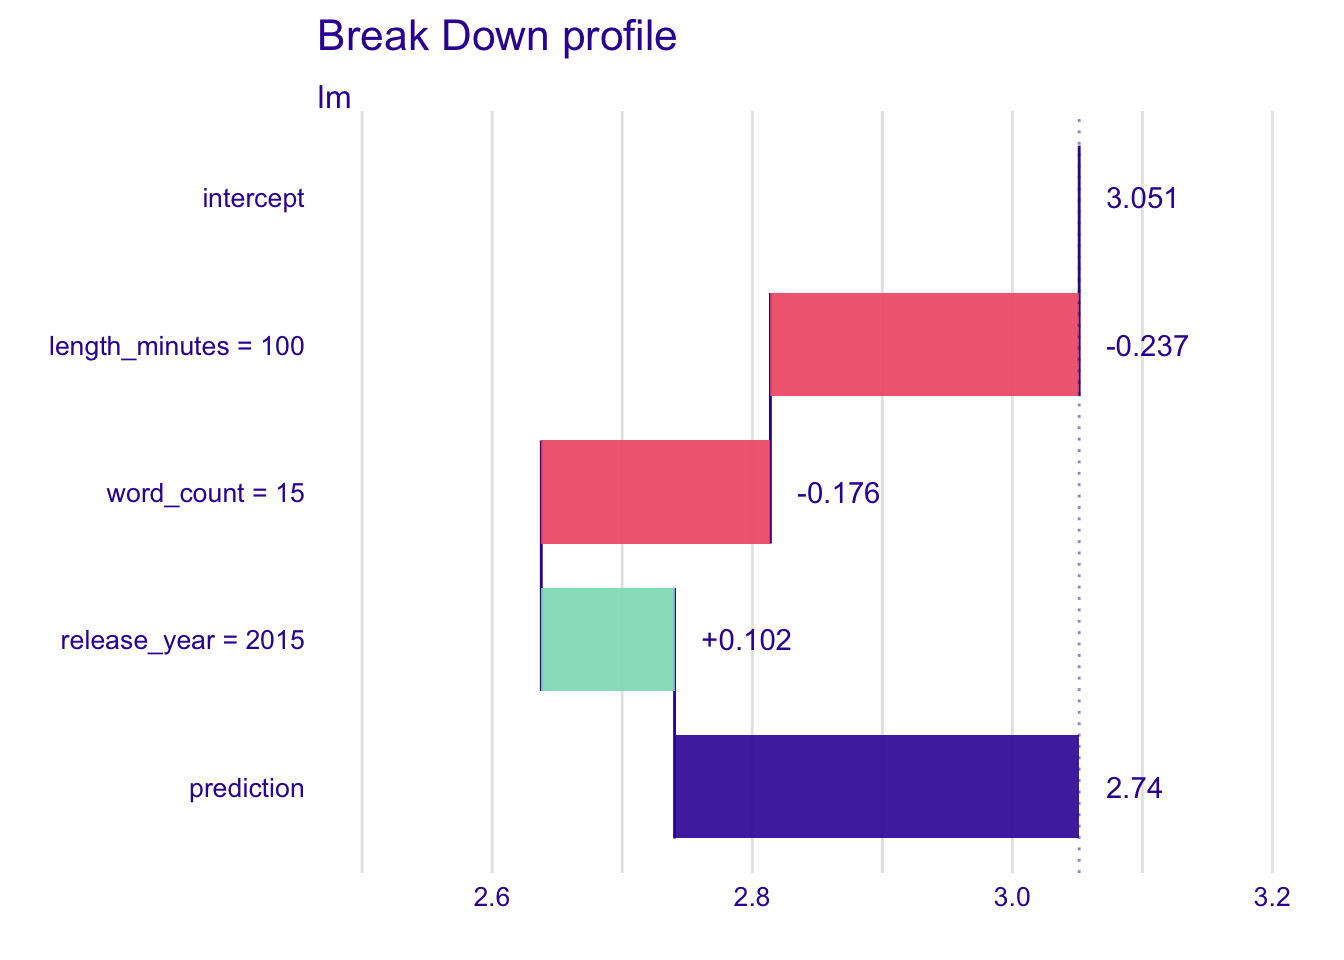
\includegraphics{model_criticism_files/figure-pdf/unnamed-chunk-36-1.pdf}

}

\end{figure}

\begin{Shaded}
\begin{Highlighting}[]
\FunctionTok{auc}\NormalTok{(roc)}
\end{Highlighting}
\end{Shaded}

\begin{verbatim}
Area under the curve: 0.9135
\end{verbatim}

\subsubsection{Python}

\begin{Shaded}
\begin{Highlighting}[]
\ImportTok{from}\NormalTok{ sklearn.metrics }\ImportTok{import}\NormalTok{ roc\_curve, auc}

\NormalTok{fpr, tpr, thresholds }\OperatorTok{=}\NormalTok{ roc\_curve(}
\NormalTok{    testing\_data.rating\_good, }
\NormalTok{    predictions}
\NormalTok{)}

\NormalTok{auc(fpr, tpr)}
\end{Highlighting}
\end{Shaded}

\begin{verbatim}
0.8314116002795248
\end{verbatim}

With ROC curves and AUC values, we can get a sense of how well our model
is able to distinguish between the two classes. Now we can find the
ideal cut-point for balancing the TPR and FPR.

\subsubsection{R}

\begin{Shaded}
\begin{Highlighting}[]
\FunctionTok{coords}\NormalTok{(roc, }\StringTok{"best"}\NormalTok{, }\AttributeTok{ret =} \StringTok{"threshold"}\NormalTok{, }\AttributeTok{transpose =} \ConstantTok{TRUE}\NormalTok{)}
\end{Highlighting}
\end{Shaded}

\begin{verbatim}
threshold 
0.6597755 
\end{verbatim}

\subsubsection{Python}

\begin{Shaded}
\begin{Highlighting}[]
\NormalTok{thresholds[np.argmax(tpr }\OperatorTok{{-}}\NormalTok{ fpr)]}
\end{Highlighting}
\end{Shaded}

\begin{verbatim}
1
\end{verbatim}

Those coordinates are going to give us the ``best'' decision cut-point.
Instead of being naive about setting our probability to .5, this will
give a cut-point that will lead to better classifications for our
testing data.

We will leave it to you to take that ideal cut-point value and update
your metrics to see how much of a difference it will make.

Whether it is a meager, modest, or meaningful improvement is going to
vary from situation to situation, as will how you determine if your
model is ``good'' or ``bad''. If we look back to our original
\texttt{Balanced\ Accuracy} value of 0.6490, we'd imagine that our model
gets a True Positive or True Negative about 65\% of the time, leaving us
wrong 35\% of the time. Is that good or bad?

\section{Model Visualizations}\label{model-visualizations}

Using various fit metrics to assess your model's performance is critical
for knowing how well it will do with new data. As good as it might be to
know if it is useful, you might also want to know what is actually
happening in the model. Which variables are important? How did a
specific observation reach its predicted value?

For these tasks, and many others, we can turn to visualizations to gain
a better understanding of our model. Afterall, we can't really criticize
something we don't understand, can we? To help us along, we are going to
use \texttt{DALEX} to create \textbf{model explainers}.

We will focus on two types of explainers: \textbf{variable importance}
and \textbf{localized predictions}. We will look at them individually
for regression and classification tasks.

\subsection{Regression}\label{regression}

We are going to add some more features to our model to make it a little
more interesting, check that model's performance, and then look at the
\textbf{Partial Dependence Plots}, which will give us a good idea about
the relationship between the features and the target.

\subsubsection{R}

\begin{Shaded}
\begin{Highlighting}[]
\FunctionTok{library}\NormalTok{(DALEX)}

\NormalTok{features }\OtherTok{\textless{}{-}} \FunctionTok{c}\NormalTok{(}
  \StringTok{"review\_year\_0"}\NormalTok{, }\StringTok{"release\_year\_0"}\NormalTok{,}
  \StringTok{"age\_sc"}\NormalTok{, }\StringTok{"length\_minutes\_sc"}\NormalTok{, }
  \StringTok{"total\_reviews\_sc"}\NormalTok{, }\StringTok{"word\_count\_sc"}\NormalTok{, }
  \StringTok{"genre"}\NormalTok{, }\StringTok{"gender"}\NormalTok{, }
  \StringTok{"reviewer\_type"}\NormalTok{, }\StringTok{"work\_status"}\NormalTok{, }
  \StringTok{"season"}\NormalTok{)}

\NormalTok{train\_explain }\OtherTok{\textless{}{-}} \FunctionTok{explain}\NormalTok{(}
\NormalTok{  model\_train, }
  \AttributeTok{data =}\NormalTok{ training\_data[, features], }
  \AttributeTok{y =}\NormalTok{ training\_data}\SpecialCharTok{$}\NormalTok{rating,}
\NormalTok{)}
\end{Highlighting}
\end{Shaded}

\begin{verbatim}
Preparation of a new explainer is initiated
  -> model label       :  lm  (  default  )
  -> data              :  750  rows  11  cols 
  -> target variable   :  750  values 
  -> predict function  :  yhat.lm  will be used (  default  )
  -> predicted values  :  No value for predict function target column. (  default  )
  -> model_info        :  package stats , ver. 4.3.2 , task regression (  default  ) 
  -> predicted values  :  numerical, min =  1.482451 , mean =  3.0464 , max =  4.601403  
  -> residual function :  difference between y and yhat (  default  )
  -> residuals         :  numerical, min =  -1.104083 , mean =  6.470611e-16 , max =  1.079547  
  A new explainer has been created!  
\end{verbatim}

\begin{Shaded}
\begin{Highlighting}[]
\NormalTok{train\_performance }\OtherTok{\textless{}{-}} \FunctionTok{model\_performance}\NormalTok{(train\_explain)}

\NormalTok{train\_performance}
\end{Highlighting}
\end{Shaded}

\begin{verbatim}
Measures for:  regression
mse        : 0.109689 
rmse       : 0.3311933 
r2         : 0.7284077 
mad        : 0.2100457

Residuals:
          0%          10%          20%          30%          40%          50%          60%          70%          80% 
-1.104083413 -0.421736455 -0.262694466 -0.159452727 -0.087410171 -0.007908602  0.081304237  0.167072295  0.258159568 
         90%         100% 
 0.437810737  1.079547137 
\end{verbatim}

\begin{Shaded}
\begin{Highlighting}[]
\NormalTok{train\_var\_effect }\OtherTok{\textless{}{-}} \FunctionTok{model\_profile}\NormalTok{(train\_explain, }
\NormalTok{                            features)}
\end{Highlighting}
\end{Shaded}

\begin{Shaded}
\begin{Highlighting}[]
\FunctionTok{plot}\NormalTok{(train\_var\_effect)}
\end{Highlighting}
\end{Shaded}

\begin{figure}[H]

{\centering \includegraphics{model_criticism_files/figure-pdf/fig-r_perf-plot-1.pdf}

}

\caption{\label{fig-r_perf-plot}R Performance Plot}

\end{figure}

\subsubsection{Python}

\begin{Shaded}
\begin{Highlighting}[]
\ImportTok{import}\NormalTok{ dalex }\ImportTok{as}\NormalTok{ dx}
\ImportTok{import}\NormalTok{ matplotlib.pyplot }\ImportTok{as}\NormalTok{ plt}

\NormalTok{train\_explain }\OperatorTok{=}\NormalTok{ dx.Explainer(}
\NormalTok{    model\_train, }
\NormalTok{    data }\OperatorTok{=}\NormalTok{ X\_features, }
\NormalTok{    y }\OperatorTok{=}\NormalTok{ training\_data.rating,}
\NormalTok{)}
\end{Highlighting}
\end{Shaded}

\begin{verbatim}
Preparation of a new explainer is initiated

  -> data              : numpy.ndarray converted to pandas.DataFrame. Columns are set as string numbers.
  -> data              : 750 rows 25 cols
  -> target variable   : Parameter 'y' was a pandas.Series. Converted to a numpy.ndarray.
  -> target variable   : 750 values
  -> model_class       : statsmodels.regression.linear_model.RegressionResultsWrapper (default)
  -> label             : Not specified, model's class short name will be used. (default)
  -> predict function  : <function yhat_default at 0x161a023e0> will be used (default)
  -> predict function  : Accepts pandas.DataFrame and numpy.ndarray.
  -> predicted values  : min = 1.51, mean = 3.05, max = 4.56
  -> model type        : regression will be used (default)
  -> residual function : difference between y and yhat (default)
  -> residuals         : min = -0.89, mean = 1.17e-16, max = 1.04
  -> model_info        : package statsmodels

A new explainer has been created!
\end{verbatim}

\begin{Shaded}
\begin{Highlighting}[]

\NormalTok{train\_performance }\OperatorTok{=}\NormalTok{ train\_explain.model\_performance()}

\NormalTok{perf\_plot }\OperatorTok{=}\NormalTok{ train\_performance.plot()}
\end{Highlighting}
\end{Shaded}

\begin{Shaded}
\begin{Highlighting}[]
\NormalTok{perf\_plot.show()}
\end{Highlighting}
\end{Shaded}

\begin{figure}

{\centering 

}

\caption{\label{fig-py_perf-plot}Python Performance Plot}

\end{figure}

We can see what R and Python offer us for model performance plots in
Figure~\ref{fig-r_perf-plot} and Figure~\ref{fig-py_perf-plot}. We can
dig into more specific information about our model, beyond just the
general performance.

\subsubsection{Variable Importance}\label{variable-importance}

As with any model, knowing which variables are important is a critical
piece of information. We can use the \texttt{model\_parts} function to
get a sense of which variables are most important to our model. Dalex
creates feature importance by assessing how a model's RMSE changes when
a feature is permuted. The more the loss changes, the more important the
feature!

\subsubsection{R}

\begin{Shaded}
\begin{Highlighting}[]
\NormalTok{model\_var\_imp }\OtherTok{\textless{}{-}} \FunctionTok{model\_parts}\NormalTok{(}
\NormalTok{  train\_explain, }\AttributeTok{type =} \StringTok{"variable\_importance"}
\NormalTok{)}
\end{Highlighting}
\end{Shaded}

\begin{Shaded}
\begin{Highlighting}[]
\FunctionTok{plot}\NormalTok{(model\_var\_imp)}
\end{Highlighting}
\end{Shaded}

\begin{figure}[H]

{\centering \includegraphics{model_criticism_files/figure-pdf/fig-r_var-imp-1.pdf}

}

\caption{\label{fig-r_var-imp}R Variable Importance Plot}

\end{figure}

\subsubsection{Python}

\begin{Shaded}
\begin{Highlighting}[]
\NormalTok{model\_var\_imp }\OperatorTok{=}\NormalTok{ train\_explain.model\_parts(}
  \BuiltInTok{type} \OperatorTok{=} \StringTok{"variable\_importance"}
\NormalTok{)}
\end{Highlighting}
\end{Shaded}

\begin{Shaded}
\begin{Highlighting}[]
\NormalTok{model\_var\_imp.plot()}
\end{Highlighting}
\end{Shaded}

In Figure~\ref{fig-r_var-imp} and \textbf{?@fig-py\_var-imp}, we see
that \texttt{total\_reviews\_sc}, \texttt{length\_minutes\_sc},
\texttt{word\_count\_sc}, and \texttt{release\_year\_0} are the most
important features in our model. Now that we know the variables that are
pulling the most weight, we can turn to exploring predictions.

\subsubsection{Localized Predictions}\label{localized-predictions}

If you are every curious to see how a particular observation reached its
predicted value, you can use the \texttt{predict\_parts} function to get
a sense of how each feature contributed to the final prediction. We will
look at the second observation in our testing\_data to see how it was
predicted.

\subsubsection{R}

\begin{Shaded}
\begin{Highlighting}[]
\NormalTok{break\_down\_plot }\OtherTok{\textless{}{-}} \FunctionTok{predict\_parts}\NormalTok{(}
\NormalTok{  train\_explain, }
  \AttributeTok{new\_observation =}\NormalTok{ testing\_data[}\DecValTok{2}\NormalTok{, ], }
  \AttributeTok{type =} \StringTok{"break\_down"}\NormalTok{)}
\end{Highlighting}
\end{Shaded}

\begin{Shaded}
\begin{Highlighting}[]
\FunctionTok{plot}\NormalTok{(break\_down\_plot)}
\end{Highlighting}
\end{Shaded}

\begin{figure}[H]

{\centering \includegraphics{model_criticism_files/figure-pdf/fig-r_break-down-1.pdf}

}

\caption{\label{fig-r_break-down}R Break Down Plot}

\end{figure}

\subsubsection{Python}

\begin{Shaded}
\begin{Highlighting}[]
\NormalTok{break\_down\_plot }\OperatorTok{=}\NormalTok{ train\_explain.predict\_parts(}
\NormalTok{    new\_observation }\OperatorTok{=}\NormalTok{ X\_features\_testing[}\DecValTok{1}\NormalTok{],}
    \BuiltInTok{type} \OperatorTok{=} \StringTok{"break\_down"}
\NormalTok{)}
\end{Highlighting}
\end{Shaded}

\begin{Shaded}
\begin{Highlighting}[]
\NormalTok{break\_down\_plot.plot()}
\end{Highlighting}
\end{Shaded}

The Break down plots in Figure~\ref{fig-r_break-down} and
\textbf{?@fig-py\_break-down} show us how each feature contributed to
the final prediction for an observation. If a prediction from a model
has ever surprised you, this is a great way to see how that prediction
actually happened!

\subsubsection{Shap Plots}\label{shap-plots}

\textbf{Shapley values} are a way to explain the predictions made by
machine learning models. They break down a prediction to show the impact
of each feature. The Shapley value was originally developed in game
theory to determine how much each player in a cooperative game has
contributed to the total payoff of the game. You'll commonly see them
used in conjunction with tree-based models, like xgboost, but they can
be used with any model.

\subsubsection{R}

\begin{Shaded}
\begin{Highlighting}[]
\NormalTok{shap\_plot }\OtherTok{\textless{}{-}} \FunctionTok{predict\_parts}\NormalTok{(}
\NormalTok{  train\_explain, }
  \AttributeTok{new\_observation =}\NormalTok{ testing\_data, }
  \AttributeTok{type =} \StringTok{"shap"}\NormalTok{)}
\end{Highlighting}
\end{Shaded}

\begin{Shaded}
\begin{Highlighting}[]
\FunctionTok{plot}\NormalTok{(shap\_plot)}
\end{Highlighting}
\end{Shaded}

\begin{figure}[H]

{\centering \includegraphics{model_criticism_files/figure-pdf/fig-r_shap-1.pdf}

}

\caption{\label{fig-r_shap}R Shap Plot}

\end{figure}

\subsubsection{Python}

\begin{Shaded}
\begin{Highlighting}[]
\NormalTok{shap\_plot }\OperatorTok{=}\NormalTok{ train\_explain.predict\_parts(}
\NormalTok{    new\_observation }\OperatorTok{=}\NormalTok{ X\_features\_testing[}\DecValTok{1}\NormalTok{], }
    \BuiltInTok{type} \OperatorTok{=} \StringTok{"shap"}
\NormalTok{)}
\end{Highlighting}
\end{Shaded}

\begin{Shaded}
\begin{Highlighting}[]
\NormalTok{shap\_plot.plot()}
\end{Highlighting}
\end{Shaded}

The Shap plots in Figure~\ref{fig-r_shap} and \textbf{?@fig-py\_shap}
show us how each feature contributed to the final prediction for an
observation.

\subsection{Classification}\label{classification-1}

The set-up and functions are exactly the same for classification models,
so we want to show you how we can also incorporate information from
categorical variables into our explainers.

We'll create our explainer and then look at the \textbf{Partial
Dependence Plots} for our model, but broken down by \texttt{genre}.

\subsubsection{R}

\begin{Shaded}
\begin{Highlighting}[]
\NormalTok{train\_explain }\OtherTok{\textless{}{-}} \FunctionTok{explain}\NormalTok{(}
\NormalTok{  logistic\_model\_train, }
  \AttributeTok{data =}\NormalTok{ training\_data[, features], }
  \AttributeTok{y =}\NormalTok{ training\_data}\SpecialCharTok{$}\NormalTok{rating\_good, }
\NormalTok{)}
\end{Highlighting}
\end{Shaded}

\begin{verbatim}
Preparation of a new explainer is initiated
  -> model label       :  lm  (  default  )
  -> data              :  750  rows  11  cols 
  -> target variable   :  750  values 
  -> predict function  :  yhat.glm  will be used (  default  )
  -> predicted values  :  No value for predict function target column. (  default  )
  -> model_info        :  package stats , ver. 4.3.2 , task classification (  default  ) 
  -> predicted values  :  numerical, min =  3.610605e-05 , mean =  0.5626667 , max =  0.9999775  
  -> residual function :  difference between y and yhat (  default  )
  -> residuals         :  numerical, min =  -0.9374073 , mean =  1.811689e-11 , max =  0.9875368  
  A new explainer has been created!  
\end{verbatim}

\begin{Shaded}
\begin{Highlighting}[]
\NormalTok{train\_performance }\OtherTok{\textless{}{-}} \FunctionTok{model\_performance}\NormalTok{(train\_explain)}

\NormalTok{train\_performance}
\end{Highlighting}
\end{Shaded}

\begin{verbatim}
Measures for:  classification
recall     : 0.8767773 
precision  : 0.8545035 
f1         : 0.8654971 
accuracy   : 0.8466667 
auc        : 0.9384392

Residuals:
          0%          10%          20%          30%          40%          50%          60%          70%          80% 
-0.937407296 -0.382320876 -0.142938052 -0.032755258 -0.003380979  0.001556029  0.016205271  0.055562102  0.156125961 
         90%         100% 
 0.357388053  0.987536826 
\end{verbatim}

\begin{Shaded}
\begin{Highlighting}[]
\NormalTok{partial\_model\_profile }\OtherTok{\textless{}{-}} \FunctionTok{model\_profile}\NormalTok{(train\_explain, }
\NormalTok{                                  features, }
                                  \AttributeTok{groups =} \StringTok{"genre"}\NormalTok{,}
                                  \AttributeTok{type =} \StringTok{"partial"}\NormalTok{)}
\end{Highlighting}
\end{Shaded}

\begin{Shaded}
\begin{Highlighting}[]
\FunctionTok{plot}\NormalTok{(partial\_model\_profile)}
\end{Highlighting}
\end{Shaded}

\begin{figure}[H]

{\centering \includegraphics{model_criticism_files/figure-pdf/fig-r_partial-plot-1.pdf}

}

\caption{\label{fig-r_partial-plot}R Partial Dependence Plot by Genre}

\end{figure}

\subsubsection{Python}

\begin{Shaded}
\begin{Highlighting}[]
\NormalTok{train\_explain }\OperatorTok{=}\NormalTok{ dx.Explainer(}
\NormalTok{    logistic\_model\_train, }
\NormalTok{    data }\OperatorTok{=}\NormalTok{ X\_features, }
\NormalTok{    y }\OperatorTok{=}\NormalTok{ training\_data.rating\_good, }
\NormalTok{)}
\end{Highlighting}
\end{Shaded}

\begin{verbatim}
Preparation of a new explainer is initiated

  -> data              : numpy.ndarray converted to pandas.DataFrame. Columns are set as string numbers.
  -> data              : 750 rows 25 cols
  -> target variable   : Parameter 'y' was a pandas.Series. Converted to a numpy.ndarray.
  -> target variable   : 750 values
  -> model_class       : statsmodels.genmod.generalized_linear_model.GLMResultsWrapper (default)
  -> label             : Not specified, model's class short name will be used. (default)
  -> predict function  : <function yhat_default at 0x161a023e0> will be used (default)
  -> predict function  : Accepts pandas.DataFrame and numpy.ndarray.
  -> predicted values  : min = 9.74e-05, mean = 0.563, max = 1.0
  -> model type        : regression will be used (default)
  -> residual function : difference between y and yhat (default)
  -> residuals         : min = -0.941, mean = 1.17e-12, max = 0.944
  -> model_info        : package statsmodels

A new explainer has been created!
\end{verbatim}

\begin{Shaded}
\begin{Highlighting}[]
\NormalTok{train\_performance }\OperatorTok{=}\NormalTok{ train\_explain.model\_performance()}

\NormalTok{partial\_model\_profile }\OperatorTok{=}\NormalTok{ train\_explain.model\_profile(}
    \BuiltInTok{type} \OperatorTok{=} \StringTok{"partial"}
\NormalTok{)}
\end{Highlighting}
\end{Shaded}

\begin{verbatim}

Calculating ceteris paribus:   0%|          | 0/25 [00:00<?, ?it/s]
Calculating ceteris paribus: 100%|##########| 25/25 [00:00<00:00, 273.18it/s]
\end{verbatim}

\begin{Shaded}
\begin{Highlighting}[]
\NormalTok{partial\_model\_profile.plot()}
\end{Highlighting}
\end{Shaded}

We can see what R and Python offer us for partial dependence plots in
Figure~\ref{fig-r_partial-plot} and \textbf{?@fig-py\_partial-plot}. In
Figure~\ref{fig-r_partial-plot}, we see those are broken down by the
different genres, allowing us to see the differences between genres.

\subsubsection{Variable Importance}\label{variable-importance-1}

We can also look at the variable importance for our classification
model. While it operates on the same principle of the regression model,
variable importance for classification models is calculated by assessing
how a model's AUC changes when a feature is permuted, as opposed to
RMSE.

\subsubsection{R}

\begin{Shaded}
\begin{Highlighting}[]
\NormalTok{model\_var\_imp }\OtherTok{\textless{}{-}} \FunctionTok{model\_parts}\NormalTok{(train\_explain, }
                             \AttributeTok{type =} \StringTok{"variable\_importance"}\NormalTok{)}
\end{Highlighting}
\end{Shaded}

\begin{Shaded}
\begin{Highlighting}[]
\FunctionTok{plot}\NormalTok{(model\_var\_imp)}
\end{Highlighting}
\end{Shaded}

\begin{figure}[H]

{\centering \includegraphics{model_criticism_files/figure-pdf/fig-r_var-imp-class-1.pdf}

}

\caption{\label{fig-r_var-imp-class}R Variable Importance Plot for
Classification}

\end{figure}

\subsubsection{Python}

\begin{Shaded}
\begin{Highlighting}[]
\NormalTok{model\_var\_imp }\OperatorTok{=}\NormalTok{ train\_explain.model\_parts(}
  \BuiltInTok{type} \OperatorTok{=} \StringTok{"variable\_importance"}
\NormalTok{  )}
\end{Highlighting}
\end{Shaded}

\begin{Shaded}
\begin{Highlighting}[]
\NormalTok{model\_var\_imp.plot()}
\end{Highlighting}
\end{Shaded}

The variable importance plots in Figure~\ref{fig-r_var-imp-class} and
\textbf{?@fig-py\_var-imp-class} show us the variables that are the most
globally important for making our classifications. How do those
variables differ from what we saw in our linear regression model?

Since we have already seen that there isn't much difference between
models with regard to producing these plots, we will leave it up to you
to produce localized plots for your classification models!

\section{Wrapping Up}\label{wrapping-up}

It is easy to get caught up in the excitement of creating a model and
then using it to make predictions. It is also easy to get caught up in
the excitement of seeing a model perform well on a test set. It is much
harder to take a step back and ask yourself, ``Is this model really
doing what I want it to do?'' You should always be looking at which
variables are pulling the most weight in your model and how predictions
are being made.

\section{Additional Resources}\label{additional-resources}

If this chapter has piqued your curiosity, we would encourage you to
check out the following resources.

Even though we did not use the \texttt{mlr3} package in this chapter,
the \textbf{Evaluation and Benchmarking} chapter of the companion book,
\href{https://mlr3book.mlr-org.com/chapters/chapter3/evaluation_and_benchmarking.html}{Applied
Machine Learning Using mlr3 in R}, offers a great conceptual take on
model metrics and evaluation.

For a more Pythonic look at model evaluation, we would highly recommend
going through the sci-kit learn documentation on
\href{https://scikit-learn.org/stable/modules/model_evaluation.html}{Model
Evaluation}. It has you absolutely covered on code examples and
concepts.

To get the most out of \texttt{DaLEX} visualizations, we would recommend
checking out Christoph Molnar's book,
\href{https://christophm.github.io/interpretable-ml-book/}{Interpretable
Machine Learning}. It is a great resource for learning more about model
explainers and how to use them.

\chapter{How do we obtain a model?}\label{how-do-we-obtain-a-model}

In our initial linear model, the key \textbf{parameters} are the
coefficients for each feature. But how do we know what the coefficients
are and come to those values? When we run a linear model using some
program function, they appear magically, but it's worth knowing a little
bit about how they come to be, so let's try and dive a little deeper!
This chapter is more involved than most of the others, and is really for
those who like to get their hands dirty. If you're not one of those
people, that's ok, you can skip this chapter and still get a lot out of
the rest of the book. But if you're curious about how things work, or
you want to be able to do more than just run a function, then we think
you'll find the following useful.

\section{Introduction to Model
Estimation}\label{introduction-to-model-estimation}

\textbf{Model estimation} is the process of finding the parameters
associated with a model that allow us to reach a particular modeling
goal. Different types of models will have different parameters to
estimate, and there are different ways to estimate them. In general
though, the goal is the same, find the set of parameters that will lead
to the best predictions under the current data modeling context.

With model estimation, we can break things down into the following
steps:

\begin{enumerate}
\def\labelenumi{\arabic{enumi}.}
\tightlist
\item
  Start with an initial guess for the parameters
\item
  Calculate the \textbf{prediction error}, or some function of it, or
  some other value that represents our model's \textbf{objective}
\item
  \textbf{Update} the guess
\item
  Repeat steps 2 \& 3 until we find a `best' guess
\end{enumerate}

Pretty straightforward, right? Well, it's not always so simple, but this
is the general idea in most applications. In this chapter, we'll show
how to do this ourselves to take away the mystery a bit from when you
run standard model functions in typical contexts. Hopefully then you'll
gain more confidence when you do use them!

\begin{tcolorbox}[enhanced jigsaw, rightrule=.15mm, opacityback=0, left=2mm, toprule=.15mm, arc=.35mm, leftrule=.75mm, bottomrule=.15mm, breakable, colback=white]

\textbf{Estimation vs.~Optimization}\vspace{2mm}

We can use \textbf{estimation} as general term for finding parameters,
while \textbf{optimization} can be seen as a term for finding parameters
that maximize or minimize some \textbf{objective function}, or even a
combination of objectives. In some cases we can estimate parameters
without optimization, because there is a known way of solving the
problem, but in most modeling situations we are going to use some
optimization approach to find a `best' set of parameters.

\end{tcolorbox}

\section{Key ideas}\label{key-ideas-2}

\begin{itemize}
\tightlist
\item
  \textbf{Parameters} are the values associated with a model
\item
  \textbf{Estimation} is the process of finding the parameters
  associated with a model
\item
  The \textbf{objective function} produces a value that we want to, for
  example, maximize or minimize
\item
  \textbf{Prediction error} is the difference between the actual value
  of the target and the predicted value of the target, and is often used
  to calculate the objective function
\item
  \textbf{Optimization} is the process of finding the parameters that
  maximize or minimize some objective function
\item
  \textbf{Model Selection} is the process of choosing the best model
  from a set of models
\end{itemize}

\section{Data Setup}\label{data-setup}

For the examples here, we'll use the world happiness dataset for the
year 2018. We'll use the happiness score as our target, and we'll use
the GDP per capita as our primary feature, though we may throw in some
others. Let's take a look at the data here, but for more information see
the \hyperref[appendix]{appendix}.

NOTE GTEXTRAS PLOT CAUSES PDF ERROR AND WILL HAVE TO BE IMPORTED AS FILE

\begin{longtable*}{lrrrr}
\toprule
term & happiness\_score & healthy\_life\_expectancy\_at\_birth & log\_gdp\_per\_capita & perceptions\_of\_corruption \\ 
\midrule
happiness\_score & NA & $0.78$ & $0.82$ & $-0.47$ \\ 
healthy\_life\_expectancy\_at\_birth & $0.78$ & NA & $0.86$ & $-0.34$ \\ 
log\_gdp\_per\_capita & $0.82$ & $0.86$ & NA & $-0.34$ \\ 
perceptions\_of\_corruption & $-0.47$ & $-0.34$ & $-0.34$ & NA \\ 
\bottomrule
\end{longtable*}

Our happiness score has values from around 3-7, life expectancy and gdp
appear to have some notable variability, and corruption perception is
skewed toward lower values. We can also see that the features and target
are correlated with each other, which is not surprising.

We'll do some minor cleaning and renaming of columns, and we'll drop any
rows with missing values. We'll also scale the features so that they are
on the same scale, which as noted in the data chapter, can help make
estimation easier.

\subsubsection{R}

\begin{Shaded}
\begin{Highlighting}[]
\NormalTok{df\_happiness }\OtherTok{\textless{}{-}} \FunctionTok{read\_csv}\NormalTok{(}\StringTok{"data/world\_happiness\_2018.csv"}\NormalTok{) }\SpecialCharTok{|\textgreater{}}
    \FunctionTok{drop\_na}\NormalTok{() }\SpecialCharTok{|\textgreater{}}
    \FunctionTok{select}\NormalTok{(}
\NormalTok{        country,}
\NormalTok{        happiness\_score,}
\NormalTok{        healthy\_life\_expectancy\_at\_birth,}
\NormalTok{        log\_gdp\_per\_capita,}
\NormalTok{        perceptions\_of\_corruption}
\NormalTok{    ) }\SpecialCharTok{|\textgreater{}}
    \FunctionTok{rename}\NormalTok{(}
        \AttributeTok{happiness  =}\NormalTok{ happiness\_score,}
        \AttributeTok{life\_exp   =}\NormalTok{ healthy\_life\_expectancy\_at\_birth,}
        \AttributeTok{log\_gdp\_pc =}\NormalTok{ log\_gdp\_per\_capita,}
        \AttributeTok{corrupt    =}\NormalTok{ perceptions\_of\_corruption}
\NormalTok{    ) }\SpecialCharTok{|\textgreater{}}
    \FunctionTok{mutate}\NormalTok{(}
        \AttributeTok{gdp\_pc =} \FunctionTok{exp}\NormalTok{(log\_gdp\_pc), }\CommentTok{\# put back on original scale before scaling}
        \FunctionTok{across}\NormalTok{(life\_exp}\SpecialCharTok{:}\NormalTok{gdp\_pc, \textbackslash{}(x) (x }\SpecialCharTok{{-}} \FunctionTok{mean}\NormalTok{(x)) }\SpecialCharTok{/} \FunctionTok{sd}\NormalTok{(x))}
\NormalTok{    ) }\SpecialCharTok{|\textgreater{}}
    \FunctionTok{select}\NormalTok{(}\SpecialCharTok{{-}}\NormalTok{log\_gdp\_pc) }\CommentTok{\# drop the log version}
\end{Highlighting}
\end{Shaded}

\subsubsection{Python}

\begin{Shaded}
\begin{Highlighting}[]
\NormalTok{df\_happiness }\OperatorTok{=}\NormalTok{ (}
\NormalTok{    pd.read\_csv(}\StringTok{\textquotesingle{}data/world\_happiness\_2018.csv\textquotesingle{}}\NormalTok{)}
\NormalTok{    .dropna()}
\NormalTok{    .rename(}
\NormalTok{        columns }\OperatorTok{=}\NormalTok{ \{}
            \StringTok{\textquotesingle{}happiness\_score\textquotesingle{}}\NormalTok{: }\StringTok{\textquotesingle{}happiness\textquotesingle{}}\NormalTok{,}
            \StringTok{\textquotesingle{}healthy\_life\_expectancy\_at\_birth\textquotesingle{}}\NormalTok{: }\StringTok{\textquotesingle{}life\_exp\textquotesingle{}}\NormalTok{,}
            \StringTok{\textquotesingle{}log\_gdp\_per\_capita\textquotesingle{}}\NormalTok{: }\StringTok{\textquotesingle{}log\_gdp\_pc\textquotesingle{}}\NormalTok{,}
            \StringTok{\textquotesingle{}perceptions\_of\_corruption\textquotesingle{}}\NormalTok{: }\StringTok{\textquotesingle{}corrupt\textquotesingle{}}
\NormalTok{        \}}
\NormalTok{    )}
\NormalTok{    .assign(}
\NormalTok{        gdp\_pc }\OperatorTok{=} \KeywordTok{lambda}\NormalTok{ x: np.exp(x[}\StringTok{\textquotesingle{}log\_gdp\_pc\textquotesingle{}}\NormalTok{]),}
\NormalTok{    )    }
\NormalTok{    [[}\StringTok{\textquotesingle{}country\textquotesingle{}}\NormalTok{, }\StringTok{\textquotesingle{}happiness\textquotesingle{}}\NormalTok{,}\StringTok{\textquotesingle{}life\_exp\textquotesingle{}}\NormalTok{, }\StringTok{\textquotesingle{}gdp\_pc\textquotesingle{}}\NormalTok{, }\StringTok{\textquotesingle{}corrupt\textquotesingle{}}\NormalTok{]]}
\NormalTok{)}


\ImportTok{from}\NormalTok{ sklearn.preprocessing }\ImportTok{import}\NormalTok{ StandardScaler}

\NormalTok{scaler }\OperatorTok{=}\NormalTok{ StandardScaler()}

\NormalTok{df\_happiness[[}\StringTok{\textquotesingle{}life\_exp\textquotesingle{}}\NormalTok{, }\StringTok{\textquotesingle{}gdp\_pc\textquotesingle{}}\NormalTok{, }\StringTok{\textquotesingle{}corrupt\textquotesingle{}}\NormalTok{]] }\OperatorTok{=}\NormalTok{ scaler.fit\_transform(}
\NormalTok{    df\_happiness[[}\StringTok{\textquotesingle{}life\_exp\textquotesingle{}}\NormalTok{, }\StringTok{\textquotesingle{}gdp\_pc\textquotesingle{}}\NormalTok{, }\StringTok{\textquotesingle{}corrupt\textquotesingle{}}\NormalTok{]]}
\NormalTok{)}
\end{Highlighting}
\end{Shaded}

\section{Starting Out by Guessing}\label{starting-out-by-guessing}

So we'll start with a model in which we predict a country's level of
happiness by their life expectancy, where if you can expect to live
longer, maybe you're probably in a country with better health care,
higher incomes, and other important stuff. We'll stick with our simple
linear model as well.

As a starting point we can just guess what the parameter should be, but
how would we know what to guess? How would we know which guesses are
better than others? Let's try a few guesses and see how they do. Let's
say that we don't think life expectancy matters, and that most countries
are at a happiness value of 4. We can plug this into the model and see
what we get:

\[
\textrm{prediction} = 4 + 0\cdot\textrm{life\_exp}
\]

Alternatively we could use the data to inform our guess. We start with a
mean of happiness score, but moving up a standard deviation of life
expectancy (roughly \textasciitilde1 years) would move a whole point of
happiness \[
\textrm{prediction} = \overline{\textrm{happiness}} + 1\cdot\textrm{life\_exp}
\]

In this case, our offset (or intercept) is the mean of the target, and
our coefficient for the scaled life expectancy is 1. This is probably a
better guess, since it is at least data driven, but it's still not
great. But how do we know it's better?

\section{Prediction Error}\label{prediction-error-1}

We can compare the predictions from each guess to the actual values of
the target. We can do this by calculating the \textbf{prediction error},
or in the context of a linear model, they are also called
\textbf{residuals}. The prediction error is the difference between the
actual value of the target and the predicted value of the target. We can
express this as:

\[
\epsilon = y - \hat{y}
\] \[ 
\textrm{error} = \textrm{target} - \textrm{(model based) guess}
\]

Not only does this tell us how far off our model prediction is, it gives
us a way to compare models. With a measure of prediction error, we can
get a \textbf{metric} for total error for all observations/predictions,
or similarly the average error. If one model or parameter set has less
total or average error, we can say it's a better model than one that has
more. Ideally we'd like to choose a model with the least error, but
we'll see that this is not always possible\footnote{It turns out that
  our error metric is itself an estimate of the true error. We'll get
  more into this later, but for now this means that we can't ever know
  the true error, and so we can't ever really know the best or true
  model. However we can still get a good or better model relative to
  others in our current data setting.}. For now, let's calculate the
error for our two guesses. One thing though, if we miss the mark above
or below our target, we still want it to count the same in terms of
prediction error. In other words, if the true happiness score is 5 and
our model predicts 5.5 or 4.5, we want those to count the same when we
total up our error\footnote{We don't have to do it this way, but it's
  the default in most scenarios. As an example, maybe for your situation
  overshooting is worse than undershooting, and so you might want to use
  an approach that would weight those errors more heavily.}. One way we
can do this is to use the squared error value, or maybe the absolute
value. We'll use squared error here, and we'll calculate the mean of the
squared errors for all our predictions. We'll do this for our two models
above.

\subsubsection{R}

\begin{Shaded}
\begin{Highlighting}[]
\NormalTok{y }\OtherTok{\textless{}{-}}\NormalTok{ df\_happiness}\SpecialCharTok{$}\NormalTok{happiness}

\CommentTok{\# Calculate the error for the guess of 4}
\NormalTok{prediction }\OtherTok{\textless{}{-}} \DecValTok{4}
\NormalTok{mse\_four }\OtherTok{\textless{}{-}} \FunctionTok{mean}\NormalTok{((y }\SpecialCharTok{{-}}\NormalTok{ prediction)}\SpecialCharTok{\^{}}\DecValTok{2}\NormalTok{)}

\CommentTok{\# Calculate the error for our other guess}
\NormalTok{prediction }\OtherTok{\textless{}{-}} \FunctionTok{mean}\NormalTok{(y) }\SpecialCharTok{+} \DecValTok{1} \SpecialCharTok{*}\NormalTok{ df\_happiness}\SpecialCharTok{$}\NormalTok{life\_exp}
\NormalTok{mse\_other }\OtherTok{\textless{}{-}} \FunctionTok{mean}\NormalTok{((y }\SpecialCharTok{{-}}\NormalTok{ prediction)}\SpecialCharTok{\^{}}\DecValTok{2}\NormalTok{)}
\end{Highlighting}
\end{Shaded}

\subsubsection{Python}

\begin{Shaded}
\begin{Highlighting}[]
\NormalTok{y }\OperatorTok{=}\NormalTok{ df\_happiness[}\StringTok{\textquotesingle{}happiness\textquotesingle{}}\NormalTok{]}

\CommentTok{\# Calculate the error for the guess of four}
\NormalTok{prediction }\OperatorTok{=} \DecValTok{4}
\NormalTok{mse\_four   }\OperatorTok{=}\NormalTok{ np.mean((y }\OperatorTok{{-}}\NormalTok{ prediction)}\OperatorTok{**}\DecValTok{2}\NormalTok{)}

\CommentTok{\# Calculate the error for our other guess}
\NormalTok{prediction }\OperatorTok{=}\NormalTok{ y.mean() }\OperatorTok{+} \DecValTok{1} \OperatorTok{*}\NormalTok{ df\_happiness[}\StringTok{\textquotesingle{}life\_exp\textquotesingle{}}\NormalTok{]}
\NormalTok{mse\_other  }\OperatorTok{=}\NormalTok{ np.mean((y }\OperatorTok{{-}}\NormalTok{ prediction)}\OperatorTok{**}\DecValTok{2}\NormalTok{)}
\end{Highlighting}
\end{Shaded}

Now let's look at our \textbf{Mean Squared Error} (MSE), and we'll also
inspect the square root of it, or the \textbf{Root Mean Squared Error},
as that puts things back on the original target scale. We also add the
\textbf{Mean Absolute Error} as another metric. Inspecting the metrics,
we can see that we are off on average by over a point for our `\#4'
model, but notably less when guessing the mean.

\begin{longtable*}{cccccc}
\toprule
Model & MSE & RMSE & MAE & RMSE \% drop & MAE \% drop \\ 
\midrule
\#4 & $3.36$ & $1.83$ & $1.52$ &  &  \\ 
Other & $0.50$ & $0.71$ & $0.58$ & 61\% & 62\% \\ 
\bottomrule
\end{longtable*}

We can see that the other model is not only better, but results in a
61\% drop in RMSE, and similar for MAE. We'd definitely prefer the other
model over the `\#4' model. Furthermore, we can see how we can compare
models in a general fashion.

Well, this is useful, and at least we can say one model is better than
another. But you're probably hoping there is an easier way to do get a
good guess for our model parameters, especially when we have possibly
dozens of features and/or parameters to keep track of, and there is!

MOVE THIS TO LATER

\begin{tcolorbox}[enhanced jigsaw, rightrule=.15mm, opacityback=0, left=2mm, toprule=.15mm, arc=.35mm, leftrule=.75mm, bottomrule=.15mm, breakable, colback=white]

\textbf{A Note on Terminology}\vspace{2mm}

The objective function is often called the \textbf{loss function}, and
sometimes the \textbf{cost function}. However, these both imply that we
are trying to minimize the function, which is not always the
case\footnotemark{}, and it's arbitrary whether you want to minimize or
maximize the function. In fact, some people will minimize the
\emph{negative} likelihood when using \emph{maximum} likelihood! As such
we'll try to stick to the more neutral term objective function, but you
may see the other terms used interchangeably in this text. In addition,
some packages will use the term \textbf{metric} to refer a value that
you might want to examine as well, or even use to compare models. For
example, the MSE is a metric, but it may also be the objective function
we are trying to minimize. Other metrics we could calculate without
being the objective might be Adjusted R-squared and median absolute
error. We could also use MSE as the objective, but use percentage drop
in error from baseline when selecting among several models that
minimized MSE. This can be very confusing when starting out! We'll try
to stick to the term \emph{metric} for additional values that we might
want to examine separate from the \emph{objective function value}.

\end{tcolorbox}

\footnotetext{You may find that some packages will only minimize (or
maximize) a function, possibly one that you come up with yourself. It'd
be nice if they did this internally, or allowed the user to specify the
direction like most packages, but you'll need to take care when
implementing your own metrics.}

\section{Ordinary Least Squares}\label{ordinary-least-squares}

For a simple linear model, we can estimate the parameters in several
ways, but the most common is to use the \textbf{Ordinary Least Squares
(OLS)} method. OLS is a method of estimating the coefficients that
minimizes the sum of the squared errors, which we've just been doing in
the previous section\footnote{Some disciplines seem confuse models with
  estimation methods and link functions. It doesn't really make sense,
  nor is informative, to call something an OLS model or a logit model.
  Many models are estimated using a least squares approach, and
  different types of models use a logit link.}. In other words, it finds
the coefficients that minimize the sum of the squared differences
between the predicted values and the actual values. We can express this
as:

\[
\textrm{Value} = \sum_{i=1}^{n} (y_i - \hat{y_i})^2
\]

Where \(y_i\) is the actual value of the target for observation \(i\),
and \(\hat{y_i}\) is the predicted value from the model. The sum of the
squared errors is also called the \textbf{residual sum of squares}
(RSS), as opposed to the total sums of squares (i.e.~the variance of the
target), and the part explained by the model (model or explained sums of
squares). The OLS method finds the coefficients that minimize the sum of
the squared differences between the predicted values and the actual
values. It's called \emph{ordinary} least squares because there are
other least squares methods - generalized least squares, weighted least
squares, and others, but we don't need to worry about that for now. What
matters is that we have a way to estimate the coefficients that
minimizes the sum of the squared errors.

The resulting value - the sum or mean of the squared errors, as we noted
can be referred to as our \textbf{objective value}, while the
\textbf{objective function} is just the process of taking the
predictions and observed target values and totaling up their squared
differences. We can use this value to find the best parameters for a
specific model, as well as compare models with different parameters,
such as a model with additional features versus one with fewer. We can
also use this value to compare different types of models that are using
the same objective function, such as a linear model and a decision tree
model.

Let's calculate the OLS estimate for our model. From our steps above, we
need guesses and a way to update them. For now, we can just provide a
bunch of guesses, and just move along from one set to the next, and
ultimately just choose whichever has the lowest value.

\subsubsection{R}

\begin{Shaded}
\begin{Highlighting}[]
\NormalTok{ols }\OtherTok{\textless{}{-}} \ControlFlowTok{function}\NormalTok{(X, y, par, }\AttributeTok{sum\_sq =} \ConstantTok{FALSE}\NormalTok{) \{}
\NormalTok{    X }\OtherTok{\textless{}{-}} \FunctionTok{cbind}\NormalTok{(}\DecValTok{1}\NormalTok{, X)}
    \CommentTok{\# Calculate the predicted values}
\NormalTok{    y\_hat }\OtherTok{\textless{}{-}}\NormalTok{ X }\SpecialCharTok{\%*\%}\NormalTok{ par }\CommentTok{\# \%*\% is matrix multiplication}

    \CommentTok{\# Calculate the error}
\NormalTok{    error }\OtherTok{\textless{}{-}}\NormalTok{ y }\SpecialCharTok{{-}}\NormalTok{ y\_hat}

    \CommentTok{\# Calculate the value as sum or mean squared error}
\NormalTok{    value }\OtherTok{\textless{}{-}} \FunctionTok{crossprod}\NormalTok{(error) }\CommentTok{\# crossprod is matrix multiplication}

    \ControlFlowTok{if}\NormalTok{ (}\SpecialCharTok{!}\NormalTok{sum\_sq) \{}
\NormalTok{        value }\OtherTok{\textless{}{-}}\NormalTok{ value }\SpecialCharTok{/} \FunctionTok{nrow}\NormalTok{(X)}
\NormalTok{    \}}

    \CommentTok{\# Return the value}
    \FunctionTok{return}\NormalTok{(value)}
\NormalTok{\}}

\CommentTok{\# create a grid of guesses}
\NormalTok{guesses }\OtherTok{\textless{}{-}} \FunctionTok{crossing}\NormalTok{(}
    \AttributeTok{b0 =} \FunctionTok{seq}\NormalTok{(}\DecValTok{1}\NormalTok{, }\DecValTok{7}\NormalTok{, }\FloatTok{0.1}\NormalTok{),}
    \AttributeTok{b1 =} \FunctionTok{seq}\NormalTok{(}\SpecialCharTok{{-}}\DecValTok{1}\NormalTok{, }\DecValTok{1}\NormalTok{, }\FloatTok{0.1}\NormalTok{)}
\NormalTok{)}

\CommentTok{\# Example for one guess}
\FunctionTok{ols}\NormalTok{(}
    \AttributeTok{X =}\NormalTok{ df\_happiness}\SpecialCharTok{$}\NormalTok{life\_exp,}
    \AttributeTok{y =}\NormalTok{ df\_happiness}\SpecialCharTok{$}\NormalTok{happiness,}
    \AttributeTok{par =} \FunctionTok{unlist}\NormalTok{(guesses[}\DecValTok{1}\NormalTok{, ])}
\NormalTok{)}
\end{Highlighting}
\end{Shaded}

\begin{verbatim}
       [,1]
[1,] 23.777
\end{verbatim}

\subsubsection{Python}

\begin{Shaded}
\begin{Highlighting}[]
\KeywordTok{def}\NormalTok{ ols(par, X, y, }\BuiltInTok{sum} \OperatorTok{=} \VariableTok{False}\NormalTok{):}
    \CommentTok{\# add a column of 1s for the intercept}
\NormalTok{    X }\OperatorTok{=}\NormalTok{ np.c\_[np.ones(X.shape[}\DecValTok{0}\NormalTok{]), X]}

    \CommentTok{\# Calculate the predicted values}
\NormalTok{    y\_hat }\OperatorTok{=}\NormalTok{ X }\OperatorTok{@}\NormalTok{ par}
    
    \CommentTok{\# Calculate the error}
\NormalTok{    value }\OperatorTok{=}\NormalTok{ np.}\BuiltInTok{sum}\NormalTok{((y }\OperatorTok{{-}}\NormalTok{ y\_hat)}\OperatorTok{**}\DecValTok{2}\NormalTok{)}
    
    \CommentTok{\# Calculate the value as sum or average}
    \ControlFlowTok{if} \KeywordTok{not} \BuiltInTok{sum}\NormalTok{:}
\NormalTok{        value }\OperatorTok{=}\NormalTok{ value }\OperatorTok{/}\NormalTok{ X.shape[}\DecValTok{0}\NormalTok{]}
    
    \CommentTok{\# Return the value}
    \ControlFlowTok{return}\NormalTok{(value)}

\CommentTok{\# create a grid of guesses}
\ImportTok{from}\NormalTok{ itertools }\ImportTok{import}\NormalTok{ product}

\NormalTok{guesses }\OperatorTok{=}\NormalTok{ pd.DataFrame(}
\NormalTok{    product(}
\NormalTok{        np.arange(}\DecValTok{1}\NormalTok{, }\DecValTok{7}\NormalTok{, }\FloatTok{0.1}\NormalTok{),}
\NormalTok{        np.arange(}\OperatorTok{{-}}\DecValTok{1}\NormalTok{, }\DecValTok{1}\NormalTok{, }\FloatTok{0.1}\NormalTok{)}
\NormalTok{    ),}
\NormalTok{    columns }\OperatorTok{=}\NormalTok{ [}\StringTok{\textquotesingle{}b0\textquotesingle{}}\NormalTok{, }\StringTok{\textquotesingle{}b1\textquotesingle{}}\NormalTok{]}
\NormalTok{)}

\CommentTok{\# Example for one guess}
\NormalTok{ols(}
\NormalTok{    par }\OperatorTok{=}\NormalTok{ guesses.iloc[}\DecValTok{0}\NormalTok{,:],}
\NormalTok{    X }\OperatorTok{=}\NormalTok{ df\_happiness[}\StringTok{\textquotesingle{}life\_exp\textquotesingle{}}\NormalTok{],}
\NormalTok{    y }\OperatorTok{=}\NormalTok{ df\_happiness[}\StringTok{\textquotesingle{}happiness\textquotesingle{}}\NormalTok{]}
\NormalTok{)}
\end{Highlighting}
\end{Shaded}

\begin{verbatim}
23.793842044979073
\end{verbatim}

Now we want to calculate the loss for each guess and find which one
gives us the minimum function value. Note that above, we could get the
total or mean squared error by setting the \texttt{sum} parameter to
\texttt{TRUE} or \texttt{FALSE}. Either is fine, but it's more common to
use the mean, which is a little more understandable - how far do our
guess deviate from the true value on average? In the following darker
suggests a better mean squared error result from our approach.

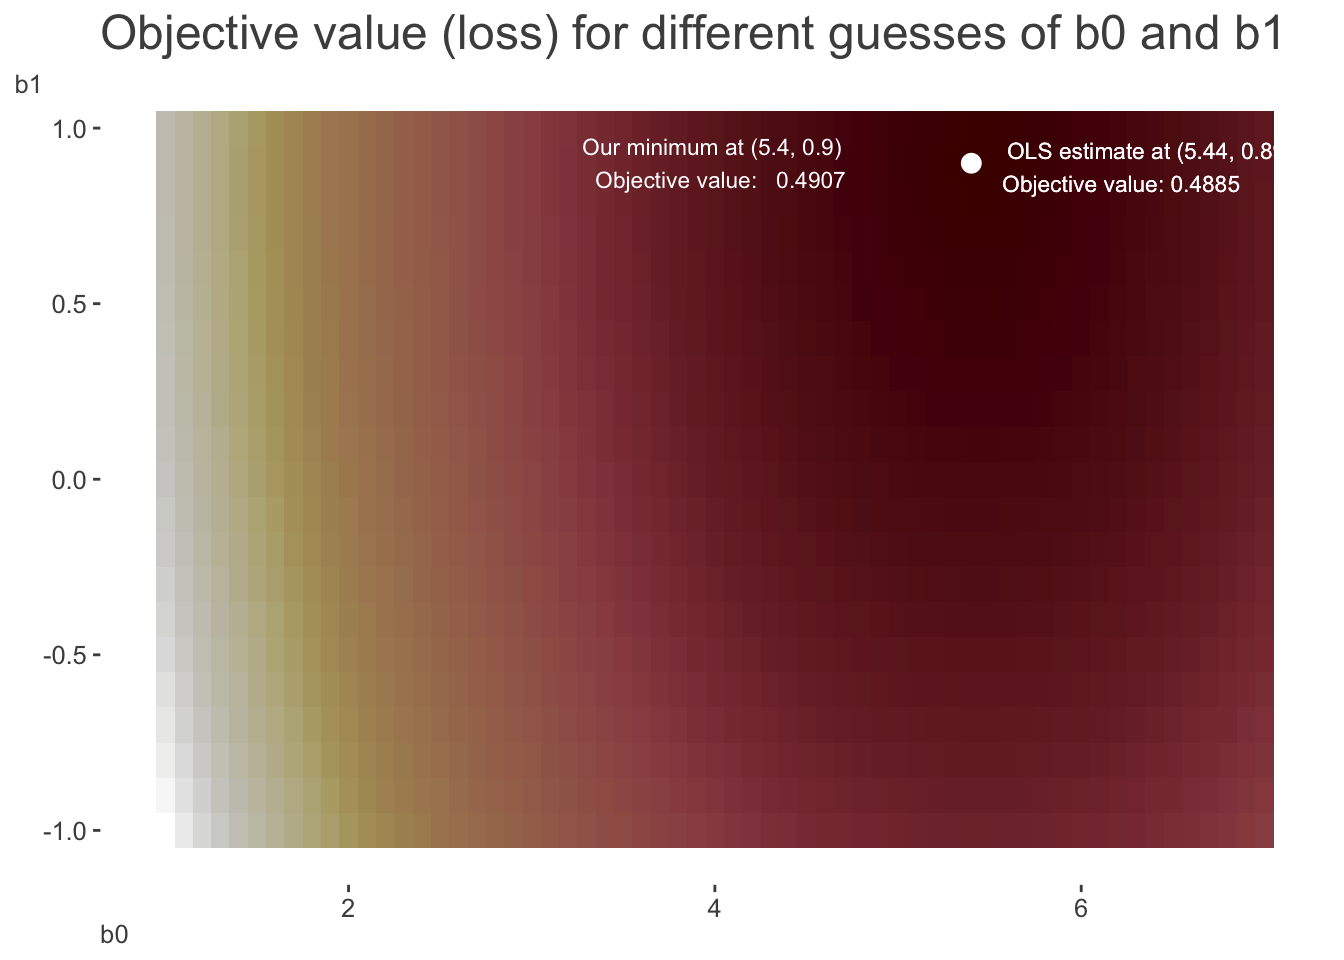
\includegraphics{estimation_files/figure-pdf/r-ols-apply-1.pdf}

If we inspect our results from the built-in functions, we had estimates
of 5.44 and 0.89 for our coefficients. These are very similar but not
exactly the same, but in the end we can see that we get pretty dang
close to what our basic \texttt{lm} or \texttt{statsmodels} functions
would get us. Pretty neat!

\begin{tcolorbox}[enhanced jigsaw, rightrule=.15mm, opacityback=0, left=2mm, toprule=.15mm, arc=.35mm, leftrule=.75mm, bottomrule=.15mm, breakable, colback=white]

\textbf{Estimation as `Learning'}\vspace{2mm}

Estimation can be seen as the process of a model learning which
parameters will best allow the predictions to match the observed data,
and hopefully, predict as-yet-unseen future data. This is a very common
way to think about estimation in machine learning, and it is a useful
way to think about our simple linear model also.

One thing to keep in mind is that it is not a magical process. It takes
good data, a good idea (model), and an appropriate estimation method to
get good results.

\end{tcolorbox}

\section{Optimization}\label{optimization}

Before we get into other objective functions, let's think about a better
way to find the best parameters for our model. Rather than just
guessing, we can use a more systematic approach, and thankfully, there
are tools out there to help us. We just use a function like our OLS
function, give it a starting point, and let the algorithms do the rest!
Thanks to some nifty approaches to making better guesses, these tools
eventually arrive at a pretty good set of parameters. Well, they usually
do, but not always- nothing's perfect! But they are pretty good, and
they are a lot better than guessing. Let's see how we can use one of
these tools to find the best parameters for our model.

Previously we created a set of guesses to search over to see which set
of parameters resulted in prediction that matched the data best. What we
did is called a \textbf{grid search}, and it is a bit of a brute force
approach to finding the best fitting model. You can imagine that a
couple of unfortunate or problematic scenarios, such as having a very
large number of parameters, or that our specified range doesn't allow us
to get to the right sets of parameters, or we specify a very large
range, but the best fitting model is within a very narrow part of that
range, such that we waste a lot of time.

In general, we can think of \textbf{optimization} as a way to find the
best parameters for our model. We start with an initial guess, see how
well it does in terms of our objective function, and then try to improve
it with a new guess. We continue to do so until a stopping point is
reached. Here is an example.

\begin{itemize}
\tightlist
\item
  \textbf{Start with an initial guess} for the parameters
\item
  Calculate the objective function given the parameters
\item
  \textbf{Update the parameters} to a new guess (that hopefully improves
  the objective function)
\item
  Calculate the objective function given the new parameters
\item
  \textbf{Repeat} until the improvement is small enough or we reach a
  maximum number of iterations we want to attempt
\end{itemize}

This is what we described before with estimation in general. The key
idea now is how we \emph{update} the old parameters with a new guess at
each iteration. Different \textbf{optimization algorithms} use different
approaches to find the updated parameters. At some point, either the
improvement is small enough, or we reach a maximum number of iterations
we want to attempt, and either of these is something we can set
ourselves. If we meet the terms of our objective, we say that we have
reached \textbf{convergence}. Sometimes, the number of iterations is not
enough for us to reach convergence, and we have to try again with a
different set of parameters, a different algorithm, maybe use some data
transformations, or something else.

So let's try it out! Both R and Python offer a function where we can
specify the objective function, and it will try to find the best
parameters for us. We'll use the \texttt{optim} function in R and the
\texttt{minimize} function in Python. It needs several inputs:

\begin{itemize}
\tightlist
\item
  the objective function
\item
  the initial guess for the parameters to get things going
\item
  inputs to the objective function
\item
  options for the optimization process, e.g.~algorithm, maximum number
  of iterations, etc.
\end{itemize}

With these inputs, we'll let the optimization functions do the rest of
the work. We'll also compare our results to the built-in functions to
make sure we're on the right track.

\subsubsection{R}

\begin{Shaded}
\begin{Highlighting}[]
\NormalTok{our\_result }\OtherTok{\textless{}{-}} \FunctionTok{optim}\NormalTok{(}
    \AttributeTok{par    =} \FunctionTok{c}\NormalTok{(}\DecValTok{1}\NormalTok{, }\DecValTok{0}\NormalTok{),}
    \AttributeTok{fn     =}\NormalTok{ ols,}
    \AttributeTok{X      =}\NormalTok{ df\_happiness}\SpecialCharTok{$}\NormalTok{life\_exp,}
    \AttributeTok{y      =}\NormalTok{ df\_happiness}\SpecialCharTok{$}\NormalTok{happiness,}
    \AttributeTok{method =} \StringTok{"BFGS"} \CommentTok{\# optimization algorithm}
\NormalTok{)}

\CommentTok{\# our\_result}
\end{Highlighting}
\end{Shaded}

\subsubsection{Python}

\begin{Shaded}
\begin{Highlighting}[]
\ImportTok{from}\NormalTok{ scipy.optimize }\ImportTok{import}\NormalTok{ minimize}

\NormalTok{our\_result }\OperatorTok{=}\NormalTok{ minimize(}
\NormalTok{    fun    }\OperatorTok{=}\NormalTok{ ols,}
\NormalTok{    x0     }\OperatorTok{=}\NormalTok{ np.array([}\FloatTok{1.}\NormalTok{, }\FloatTok{0.}\NormalTok{]),}
\NormalTok{    args   }\OperatorTok{=}\NormalTok{ (np.array(df\_happiness[}\StringTok{\textquotesingle{}life\_exp\textquotesingle{}}\NormalTok{]), np.array(df\_happiness[}\StringTok{\textquotesingle{}happiness\textquotesingle{}}\NormalTok{])),}
\NormalTok{    method }\OperatorTok{=} \StringTok{\textquotesingle{}BFGS\textquotesingle{}} \CommentTok{\# optimization algorithm}
\NormalTok{)}

\CommentTok{\# our\_result}
\end{Highlighting}
\end{Shaded}

\hypertarget{tbl-r-optim-ols}{}
\begin{longtable}{lrr}
\caption{\label{tbl-r-optim-ols}Comparison of our results to built-in function }\tabularnewline

\toprule
Parameter & Built-in & Our Result \\ 
\midrule
Intercept & $5.4450$ & $5.4450$ \\ 
Life Exp. Coef. & $0.8880$ & $0.8880$ \\ 
Objective/MSE & $0.4890$ & $0.4890$ \\ 
\bottomrule
\end{longtable}

So our little function and the right tool allows us to come up with the
same thing as base R and \texttt{statsmodels}! I hope you're feeling
pretty good at this point because you should! You just proved you could
do what seems like magic, but really all it took is just a little
knowledge about some key concepts. Let's try some more!

\section{Maximum Likelihood}\label{maximum-likelihood}

In our example thus far, we have been minimizing the specific objective
(or loss) function, which basically takes our parameter estimates,
produces a prediction, and returns the sum or mean of the squared
errors. But this is just one approach we could take. Now we'd like you
to think about the \textbf{data generating process}. We have a model
that says happiness is a function of life expectancy, but more
specifically, let's think about how the observed value of the happiness
score is generated in a statistical sense. In particular, what kind of
probability distribution might be involved? Ignoring the model, we might
think that each happiness value is generated by some random process, and
that the process is the same for each observation. Let's assume that
random process is a normal distribution. So something like this would
describe it mathematically:

\[
\textrm{happiness} \sim N(\mu, \sigma)
\]

where \(\mu\) is the mean of the happiness and \(\sigma\) is the
standard deviation, or in other words, we can think of happiness as a
random variable that is drawn from a normal distribution with \(\mu\)
and \(\sigma\) as the parameters of that distribution.

Let's apply this idea to our linear model setting. In this case, the
mean is a function of life expectancy, and we're not sure what the
standard deviation is, but we can go ahead and write our model as
follows.

\[
\mu = \beta_0 + \beta_1 * \textrm{life\_exp}
\] \[
\textrm{happiness} \sim N(\mu, \sigma)
\]

Now, we can think of the model as a way to estimate the parameters of
the normal distribution, but we have an additional parameter to
estimate. We still have our previous coefficients, but now we need to
estimate \(\sigma\), which is basically our RMSE, as well. But we still
have to think of things a little differently. When we compare our
prediction to the observed value, we don't look at the simple
difference, but we are still interested in the discrepancy between the
two. So now we think about the \textbf{likelihood} of observing the
happiness score given our prediction, which is based on the estimated
parameters, i.e.~given the \(\mu\) and \(\sigma\), and \(\mu\) is a
function of the coefficients and life expectancy. We can write this as:

\[
\textrm{Pr}(\textrm{happiness} \mid \textrm{life\_exp}, \beta_0, \beta_1, \sigma)
\]

\[
\textrm{Pr}(\textrm{happiness} \mid \mu, \sigma)
\]

Even more generally, the likelihood gives us a sense of the probability
given the parameter estimates \(\theta\). \[
\textrm{Pr}(\textrm{Data} \mid \theta)
\]

Here is a simple code demo to get a likelihood in the context of our
model. The values you see are referred to statistically as probability
density values, and they are technically not probabilities, but rather
the probability density, or \textbf{relative likelihood}, at that
observation\footnote{The actual probability of a \emph{specific value}
  is 0, but the probability of a range of values is not 0. You can find
  out more about likelihoods and probabilities at the discussion
  \href{https://stats.stackexchange.com/questions/2641/what-is-the-difference-between-likelihood-and-probability}{here},
  but in general many traditional statistical texts will have a
  discussion of this.}. For your conceptual understanding, if it makes
it easier, you can think of them in the same was as you do
probabilities, but just know that technically they are not.

\subsubsection{R}

UPDATE VALUES WHEN DEMO IS SETTLED

\begin{Shaded}
\begin{Highlighting}[]
\CommentTok{\# two example life expectancy scores, mean and 1 sd above}
\NormalTok{life\_expectancy }\OtherTok{\textless{}{-}} \FunctionTok{c}\NormalTok{(}\DecValTok{0}\NormalTok{, }\DecValTok{1}\NormalTok{)}

\CommentTok{\# observed happiness scores}
\NormalTok{happiness }\OtherTok{\textless{}{-}} \FunctionTok{c}\NormalTok{(}\DecValTok{4}\NormalTok{, }\FloatTok{5.2}\NormalTok{)}

\CommentTok{\# predicted happiness with rounded coefs}
\NormalTok{mu }\OtherTok{\textless{}{-}} \DecValTok{5} \SpecialCharTok{+} \DecValTok{1} \SpecialCharTok{*}\NormalTok{ life\_expectancy}

\CommentTok{\# just a guess for sigma}
\NormalTok{sigma }\OtherTok{\textless{}{-}}\NormalTok{ .}\DecValTok{5}

\CommentTok{\# likelihood for each observation}
\NormalTok{L }\OtherTok{\textless{}{-}} \FunctionTok{dnorm}\NormalTok{(happiness, }\AttributeTok{mean =}\NormalTok{ mu, }\AttributeTok{sd =}\NormalTok{ sigma)}
\NormalTok{L}
\end{Highlighting}
\end{Shaded}

\begin{verbatim}
[1] 0.1079819 0.2218417
\end{verbatim}

\subsubsection{Python}

\begin{Shaded}
\begin{Highlighting}[]
\ImportTok{from}\NormalTok{ scipy.stats }\ImportTok{import}\NormalTok{ norm}

\CommentTok{\# two example life expectancy scores, mean and 1 sd above}
\NormalTok{life\_expectancy }\OperatorTok{=}\NormalTok{ np.array([}\DecValTok{0}\NormalTok{, }\DecValTok{1}\NormalTok{])}

\CommentTok{\# observed happiness scores}
\NormalTok{happiness }\OperatorTok{=}\NormalTok{ np.array([}\DecValTok{4}\NormalTok{, }\FloatTok{5.2}\NormalTok{])}

\CommentTok{\# predicted happiness with rounded coefs}
\NormalTok{mu }\OperatorTok{=} \DecValTok{5} \OperatorTok{+} \DecValTok{1} \OperatorTok{*}\NormalTok{ life\_expectancy}

\CommentTok{\# just a guess for sigma}
\NormalTok{sigma }\OperatorTok{=} \FloatTok{.5}

\CommentTok{\# likelihood for each observation}
\NormalTok{L }\OperatorTok{=}\NormalTok{ norm.pdf(happiness, loc }\OperatorTok{=}\NormalTok{ mu, scale }\OperatorTok{=}\NormalTok{ sigma)}
\NormalTok{L}
\end{Highlighting}
\end{Shaded}

\begin{verbatim}
array([0.10798193, 0.22184167])
\end{verbatim}

Given a guess at the parameters, and an assumption about the
distribution of the data, we can calculate the likelihood of observing
each data point, and total those sum those up, just like we did with our
squared errors. In theory, we'd deal with the product of each
likelihood, but in practice we sum the log of the likelihood, otherwise
values would get too small for our computers to handle. Here is a
corresponding function we can use to calculate the likelihood of the
data given our parameters. Note that the actual likelihood value
returned isn't really interpretable, we just use it to compare models
with different sets of parameter guesses. Even if our total likelihoods
under comparison are negative, we prefer the model with the relatively
higher likelihood. As we just demonstrated, we'll use \texttt{optim} to
help us get good guesses\footnote{Those who have experience here will
  notice we aren't putting a lower bound on sigma. You typically want to
  do this otherwise you may get nonsensical results. You can do this by
  using the \texttt{lower} parameter in \texttt{optim} with an algorithm
  that uses boundaries, or even more simply by exponentiating the
  parameter, i.e.~\texttt{exp(par{[}1{]})}. Just remember that the
  returned value will be on the log scale, so you'll have to
  exponentiate to get to the correct scale. We leave this detail out of
  the code for now to keep things simple.}.

\subsubsection{R}

\begin{Shaded}
\begin{Highlighting}[]
\NormalTok{likelihood }\OtherTok{\textless{}{-}} \ControlFlowTok{function}\NormalTok{(par, X, y) \{}
\NormalTok{    X }\OtherTok{\textless{}{-}} \FunctionTok{cbind}\NormalTok{(}\DecValTok{1}\NormalTok{, X)}
    \CommentTok{\# setup}
\NormalTok{    beta }\OtherTok{\textless{}{-}}\NormalTok{ par[}\SpecialCharTok{{-}}\DecValTok{1}\NormalTok{] }\CommentTok{\# coefficients}
\NormalTok{    sigma }\OtherTok{\textless{}{-}} \FunctionTok{exp}\NormalTok{(par[}\DecValTok{1}\NormalTok{]) }\CommentTok{\# error sd, exp keeps positive}

\NormalTok{    N }\OtherTok{\textless{}{-}} \FunctionTok{nrow}\NormalTok{(X)}

\NormalTok{    LP }\OtherTok{\textless{}{-}}\NormalTok{ X }\SpecialCharTok{\%*\%}\NormalTok{ beta }\CommentTok{\# linear predictor}
\NormalTok{    mu }\OtherTok{\textless{}{-}}\NormalTok{ LP }\CommentTok{\# identity link in the glm sense}

    \CommentTok{\# calculate (log) likelihood}
\NormalTok{    ll }\OtherTok{\textless{}{-}} \FunctionTok{dnorm}\NormalTok{(y, }\AttributeTok{mean =}\NormalTok{ mu, }\AttributeTok{sd =}\NormalTok{ sigma, }\AttributeTok{log =} \ConstantTok{TRUE}\NormalTok{)}
    \SpecialCharTok{{-}}\FunctionTok{sum}\NormalTok{(ll) }\CommentTok{\# for minimization}
\NormalTok{\}}


\NormalTok{our\_result }\OtherTok{\textless{}{-}} \FunctionTok{optim}\NormalTok{(}
    \AttributeTok{par =} \FunctionTok{c}\NormalTok{(}\DecValTok{1}\NormalTok{, }\DecValTok{0}\NormalTok{, }\DecValTok{0}\NormalTok{),}
    \AttributeTok{fn  =}\NormalTok{ likelihood,}
    \AttributeTok{X   =}\NormalTok{ df\_happiness}\SpecialCharTok{$}\NormalTok{life\_exp,}
    \AttributeTok{y   =}\NormalTok{ df\_happiness}\SpecialCharTok{$}\NormalTok{happiness}
\NormalTok{)}

\CommentTok{\# our\_result}
\end{Highlighting}
\end{Shaded}

\subsubsection{Python}

\begin{Shaded}
\begin{Highlighting}[]
\KeywordTok{def}\NormalTok{ likelihood(par, X, y):}
    \CommentTok{\# add a column of 1s for the intercept}
\NormalTok{    X }\OperatorTok{=}\NormalTok{ np.c\_[np.ones(X.shape[}\DecValTok{0}\NormalTok{]), X]}

    \CommentTok{\# setup}
\NormalTok{    beta   }\OperatorTok{=}\NormalTok{ par[}\DecValTok{1}\NormalTok{:]         }\CommentTok{\# coefficients}
\NormalTok{    sigma  }\OperatorTok{=}\NormalTok{ np.exp(par[}\DecValTok{0}\NormalTok{])  }\CommentTok{\# error sd, exp keeps positive}

\NormalTok{    N }\OperatorTok{=}\NormalTok{ X.shape[}\DecValTok{0}\NormalTok{]}

\NormalTok{    LP }\OperatorTok{=}\NormalTok{ X }\OperatorTok{@}\NormalTok{ beta          }\CommentTok{\# linear predictor}
\NormalTok{    mu }\OperatorTok{=}\NormalTok{ LP                }\CommentTok{\# identity link in the glm sense}

    \CommentTok{\# calculate (log) likelihood}
\NormalTok{    ll }\OperatorTok{=}\NormalTok{ norm.logpdf(y, loc }\OperatorTok{=}\NormalTok{ mu, scale }\OperatorTok{=}\NormalTok{ sigma) }
    \ControlFlowTok{return}\NormalTok{(}\OperatorTok{{-}}\NormalTok{np.}\BuiltInTok{sum}\NormalTok{(ll))}

\NormalTok{our\_result }\OperatorTok{=}\NormalTok{ minimize(}
\NormalTok{    fun  }\OperatorTok{=}\NormalTok{ likelihood,}
\NormalTok{    x0   }\OperatorTok{=}\NormalTok{ np.array([}\DecValTok{1}\NormalTok{, }\DecValTok{0}\NormalTok{, }\DecValTok{0}\NormalTok{]),}
\NormalTok{    args }\OperatorTok{=}\NormalTok{ (np.array(df\_happiness[}\StringTok{\textquotesingle{}life\_exp\textquotesingle{}}\NormalTok{]), np.array(df\_happiness[}\StringTok{\textquotesingle{}happiness\textquotesingle{}}\NormalTok{]))}
\NormalTok{)}
\end{Highlighting}
\end{Shaded}

How would we switch to a maximum likelihood approach using readily
available functions? In both R and Python you can switch to using
\texttt{glm} and \texttt{GLM} respectively would be the place to start.
We can use different likelihoods distributions corresponding to the
binomial, poisson and others. Still other packages would allow even more
distributions for consideration. In general, we choose a distribution
that we feel best reflects the data generating process. For binary
targets for example, we typically would feel a bernoulli or binomial
distribution is appropriate. For count data, we might choose a poisson
or negative binomial distribution. For targets that fall between 0 and
1, we might go for a beta distribution. There are many distributions,
and even when some might feel more appropriate, we might choose another
for convenience. Some distributions tend toward a normal (a.k.a.
gaussian) distribution depending on various factors, while others are
special cases of more general distributions. For example, the
exponential distribution is a special case of the gamma distribution,
and a cauchy is equivalent to a t distribution with 1 degree of freedom,
and the t tends toward a normal with increasing degrees of freedom. Here
is a visualization of the relationships among some of the more common
distributions.

\begin{figure}

{\centering 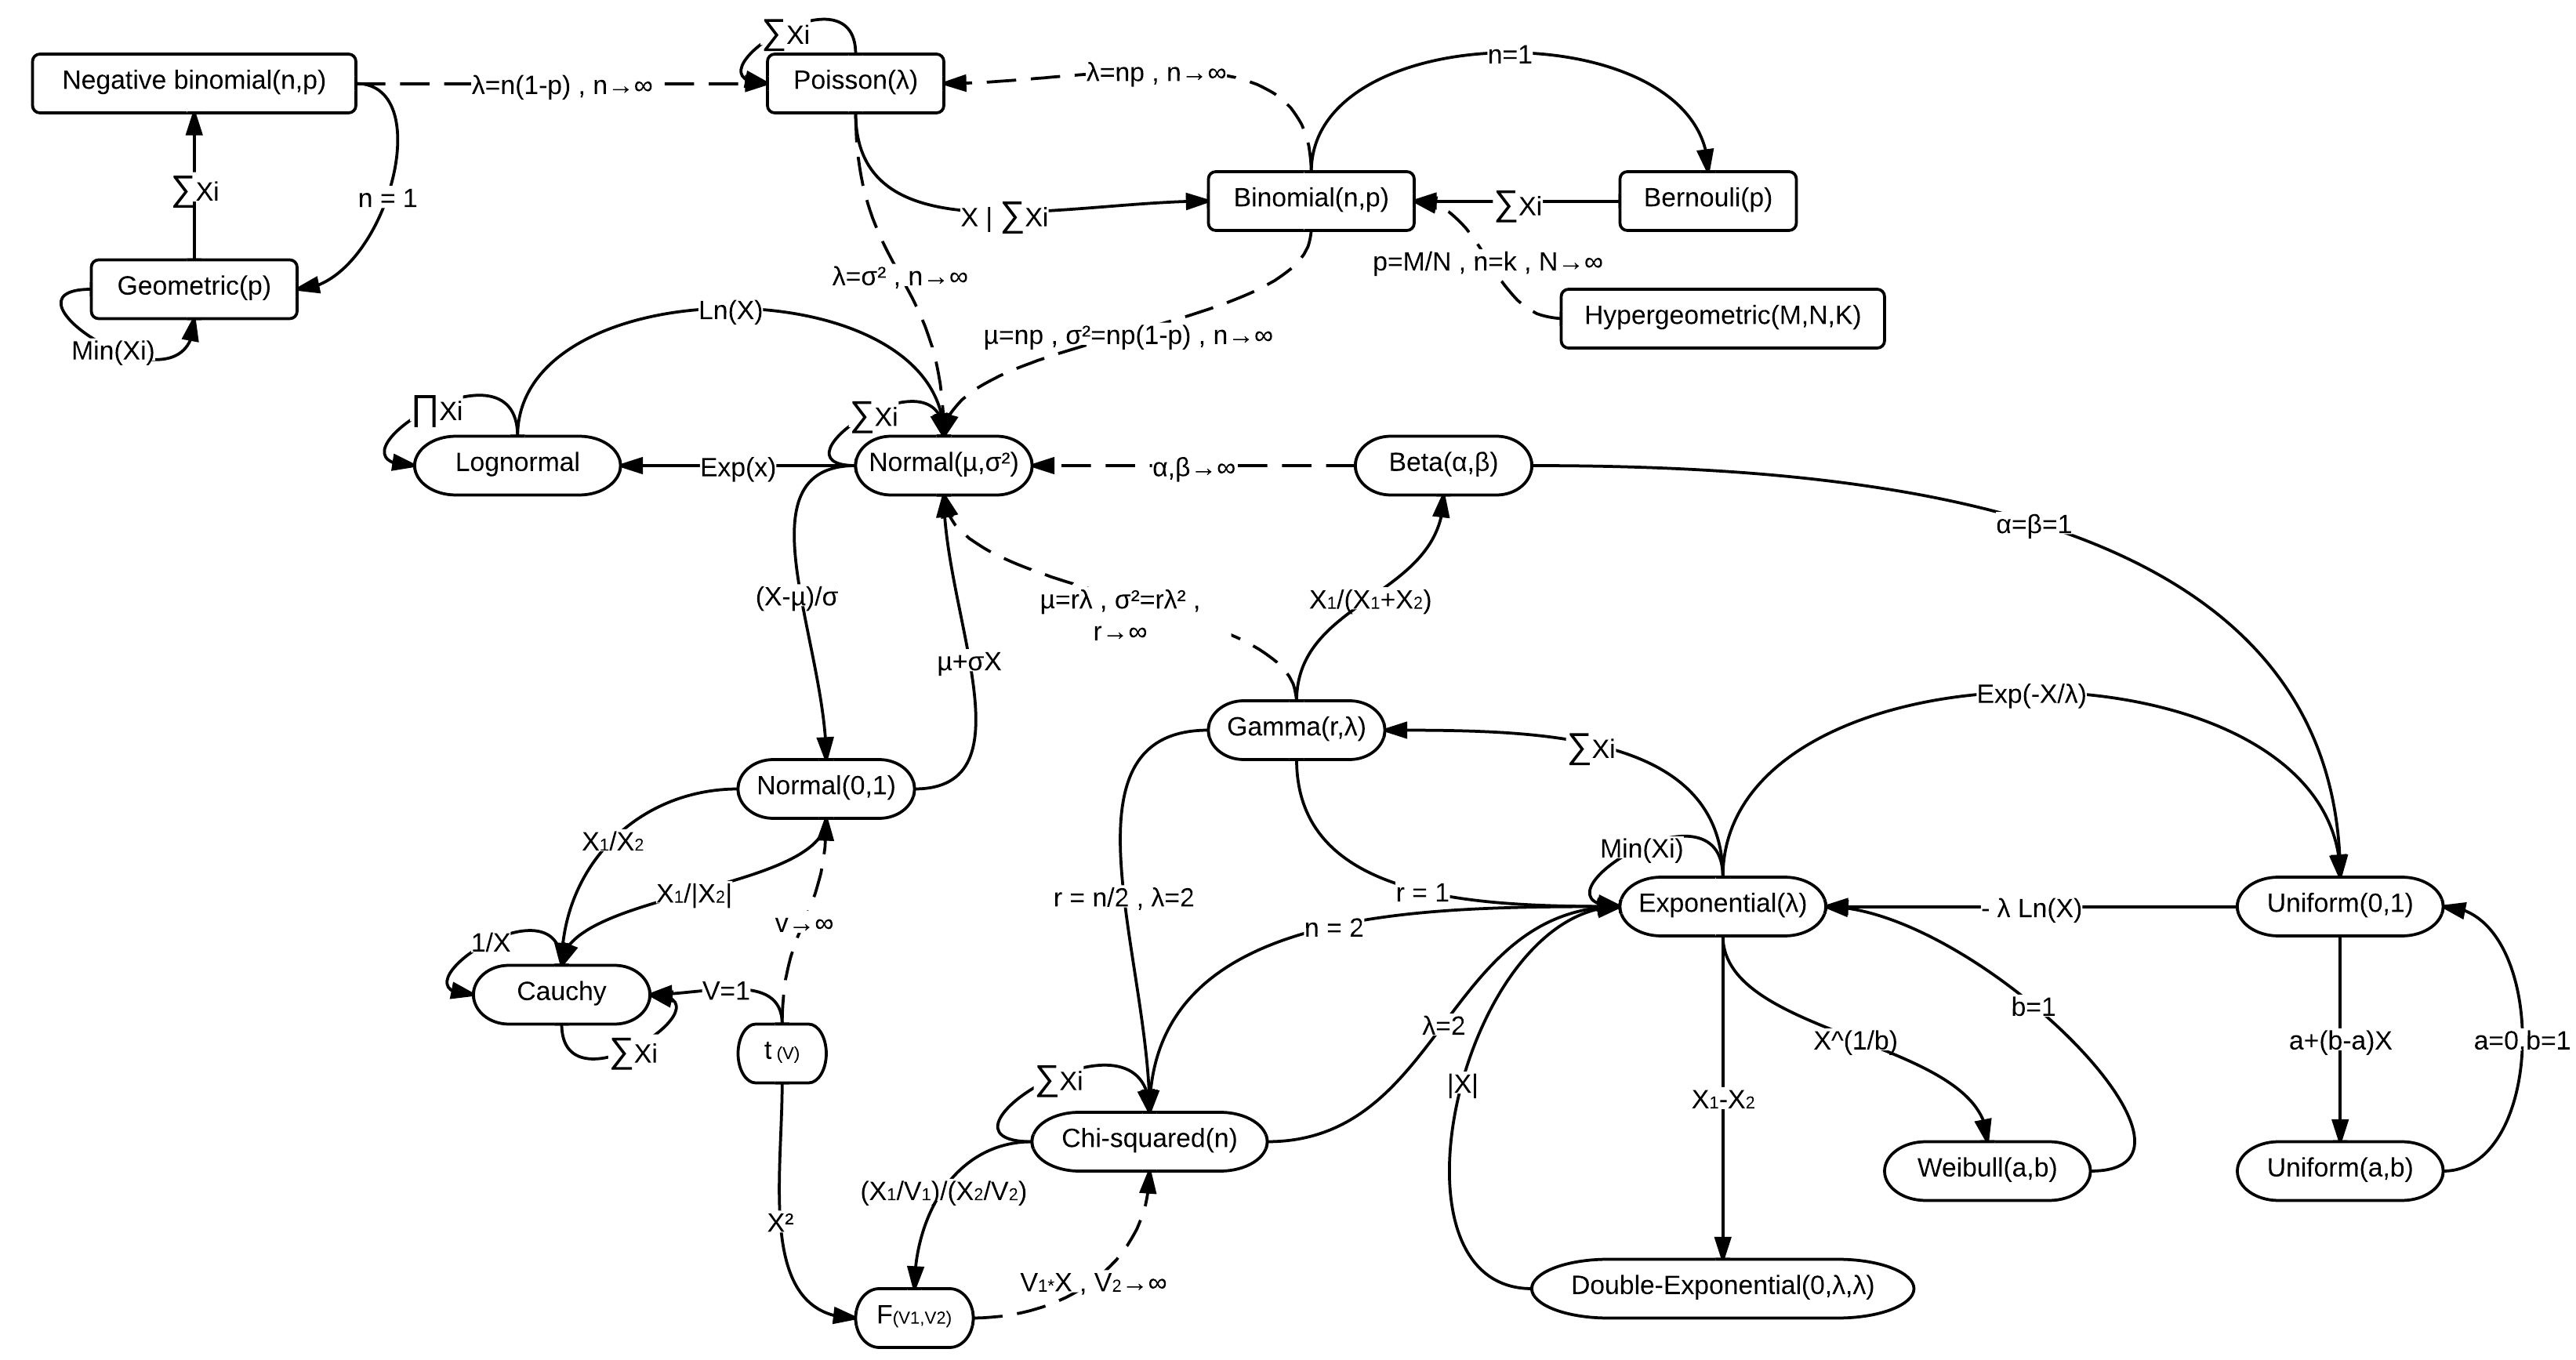
\includegraphics[width=10.95in,height=\textheight]{img/distribution_relationships.jpg}

}

\caption{\label{fig-distribution-relationships}Relationships among some
of univariate probability distributions. Image from
\href{https://en.wikipedia.org/wiki/File:Relationships_among_some_of_univariate_probability_distributions.jpg}{Wikipedia}}

\end{figure}

Here are examples of standard GLM functions in R and Python

\subsubsection{R}

\begin{Shaded}
\begin{Highlighting}[]
\FunctionTok{glm}\NormalTok{(happiness }\SpecialCharTok{\textasciitilde{}}\NormalTok{ life\_exp, }\AttributeTok{data =}\NormalTok{ df\_happiness, }\AttributeTok{family =}\NormalTok{ gaussian)}
\FunctionTok{glm}\NormalTok{(binary\_target }\SpecialCharTok{\textasciitilde{}}\NormalTok{ x1 }\SpecialCharTok{+}\NormalTok{ x2, }\AttributeTok{data =}\NormalTok{ some\_data, }\AttributeTok{family =}\NormalTok{ binomial)}
\FunctionTok{glm}\NormalTok{(count }\SpecialCharTok{\textasciitilde{}}\NormalTok{ x1 }\SpecialCharTok{+}\NormalTok{ x2, }\AttributeTok{data =}\NormalTok{ some\_data, }\AttributeTok{family =}\NormalTok{ poisson)}
\end{Highlighting}
\end{Shaded}

\subsubsection{Python}

\begin{Shaded}
\begin{Highlighting}[]
\ImportTok{import}\NormalTok{ statsmodels.formula.api }\ImportTok{as}\NormalTok{ smf}

\NormalTok{smf.glm(}\StringTok{\textquotesingle{}happiness \textasciitilde{} life\_exp\textquotesingle{}}\NormalTok{, data }\OperatorTok{=}\NormalTok{ df\_happiness, family }\OperatorTok{=}\NormalTok{ sm.families.Gaussian())}
\NormalTok{smf.glm(}\StringTok{\textquotesingle{}binary\_target \textasciitilde{} x1 + x2\textquotesingle{}}\NormalTok{, data }\OperatorTok{=}\NormalTok{ some\_data, family }\OperatorTok{=}\NormalTok{ sm.families.Binomial())}
\NormalTok{smf.glm(}\StringTok{\textquotesingle{}count \textasciitilde{} x1 + x2\textquotesingle{}}\NormalTok{, data }\OperatorTok{=}\NormalTok{ some\_data, family }\OperatorTok{=}\NormalTok{ sm.families.Poisson())}
\end{Highlighting}
\end{Shaded}

With that in mind, we can compare our result to a built-in function that
has capabilities beyond OLS. As before, we're duplicating the basic glm
result. We show more decimal places on the log likelihood estimate to
prove we aren't getting \emph{exactly} the same result

\begin{table}

\caption{\label{tbl-r-likelihood}\textbf{?(caption)}}\begin{minipage}[t]{\linewidth}
\subcaption{\label{tbl-r-likelihood-1}}

{\centering 

\setlength{\LTpost}{0mm}
\begin{longtable*}{lrr}
\toprule
Parameter & Built-in & Our Result \\ 
\midrule
Intercept & $5.44$ & $5.44$ \\ 
Life Exp. Coef. & $0.89$ & $0.89$ \\ 
Sigma & $0.71$ & $0.70$\textsuperscript{\textit{1}} \\ 
LogLik (neg) & $118.80$ & $118.80$ \\ 
\bottomrule
\end{longtable*}
\begin{minipage}{\linewidth}
\textsuperscript{\textit{1}}Parameter estimate is exponentiated\\
\end{minipage}

}

\end{minipage}%

\end{table}

Let's think more about what's going on here. It turns out that our
objective function defines a space or surface. We can think of it as a
landscape, and we are trying to find the lowest point on that landscape.
We can then think of our guesses as points on that landscape, and we are
trying to find the lowest point. Let's start get a sense of this with
the following visualization, based on a single parameter. The data is
drawn from Poisson distributed variable with true mean \(\theta=5\). We
note the calculated likelihood increases as we estimate values for
\(\theta\) closer to \(5\), or more precisely, whatever the mean
observed value is for the data. However, with more and more data, the
final ML estimate will converge on the true value. Model estimation
finds that maximum on the curve, and optimization algorithms are the
means to find it.

\begin{figure}

{\centering 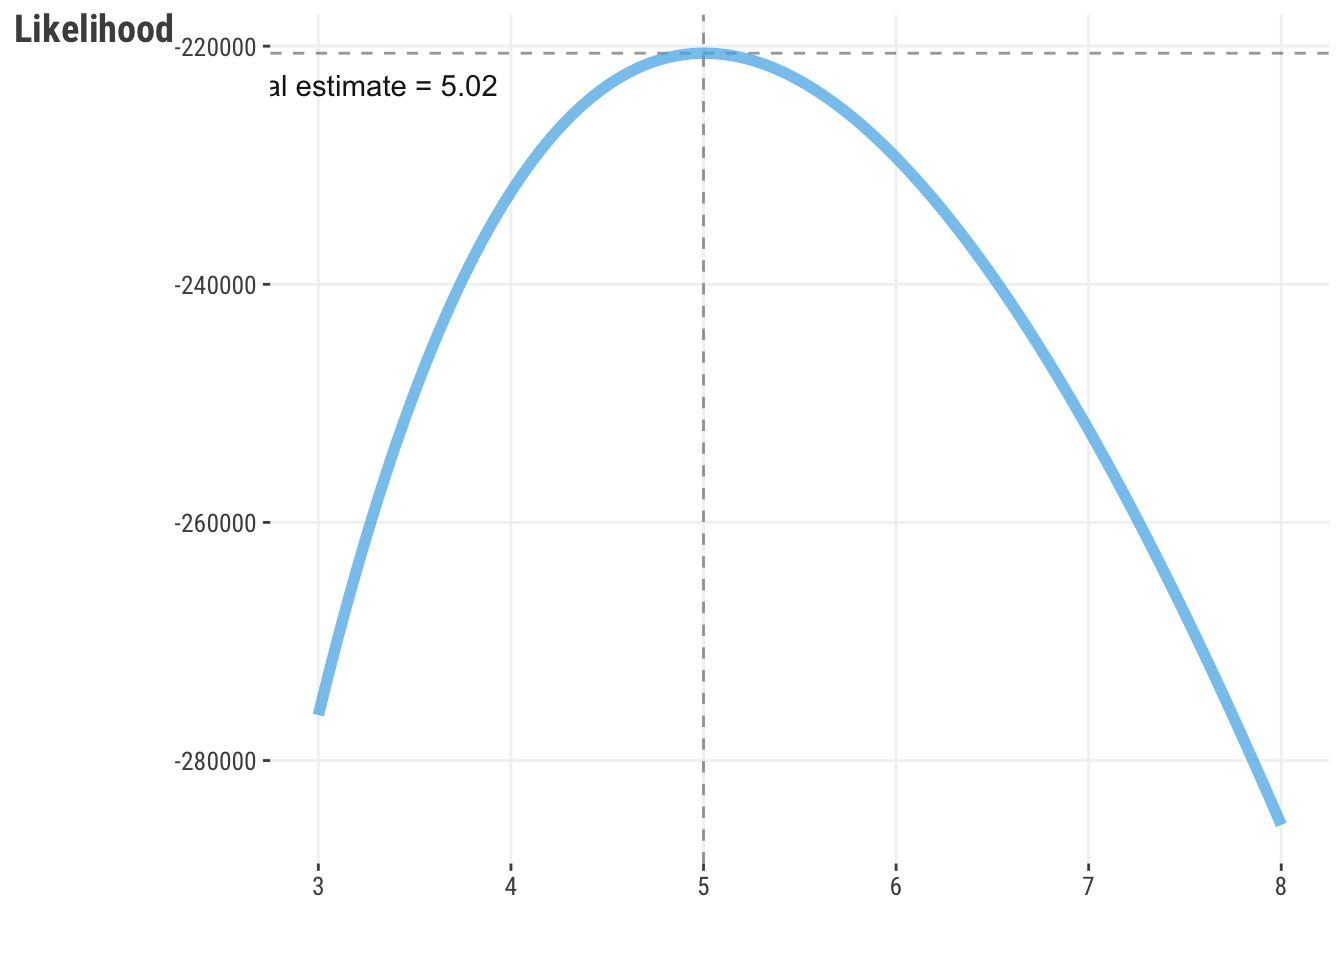
\includegraphics{estimation_files/figure-pdf/fig-r-likelihood-plot-1.pdf}

}

\caption{\label{fig-r-likelihood-plot}Likelihood function one parameter}

\end{figure}

Now let's add a parameter. If we have more than one parameter, we now
have a surfaace to deal with. Given some starting point, an optimization
procedure then travels along the surface looking for a minimum/maximum
point. For simpler settings such as this, we can visualize the
likelihood surface and its minimum point. However, even our simple demo
model has three parameters plus the likelihood, so would be difficult to
visualize without additional complexity. To get around this, we show the
results for an alternate model where happiness is standardized also,
which means the intercept is zero\footnote{Linear regression will settle
  on a line that cuts through the means, and when standardizing the mean
  of the features and target are both zero, so the line goes through the
  origin.}, and we don't have to show that.

CANT DO INTERACTIVE WITH PDF/LATEX. NEED WORKAROUND.

\begin{figure}

{\centering \includegraphics{estimation_files/figure-pdf/fig-r-likelihood-plot-3d-1.pdf}

}

\caption{\label{fig-r-likelihood-plot-3d}Likelihood surface with two
parameters}

\end{figure}

We can also see the path our estimates take, starting at a rather poor
point, but quickly updating to better values. We also see little
exploratory jumps creating a star like pattern, before things ultimately
settle to the best values. In general, these updates and paths are
dependent on the optimization algorithm one uses.

\begin{figure}

{\centering 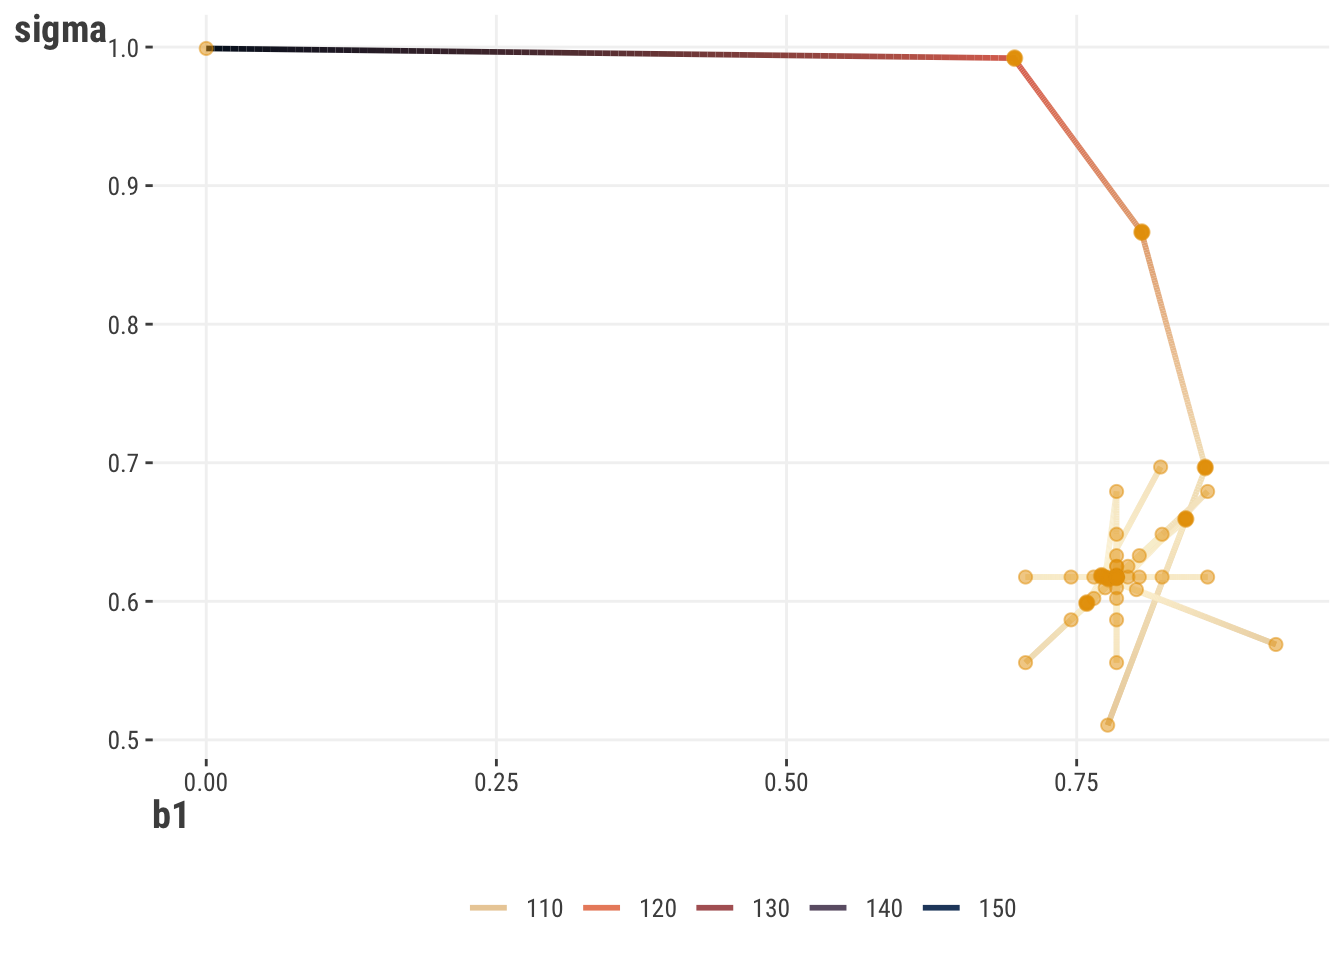
\includegraphics{estimation_files/figure-pdf/fig-r-likelihood-path-1.pdf}

}

\caption{\label{fig-r-likelihood-path}Optimization path two parameters}

\end{figure}

It turns out that in the case of a normal distribution, the maximum
likelihood estimate of the standard deviation is the estimate as the
standard deviation of the residuals. Furthermore, the maximum likelihood
estimates and OLS estimates converge to the same estimates as the sample
size increases. For any data of significance, these estimates are
indistinguishable, and the OLS estimate is the maximum likelihood
estimate for linear regression.

\subsubsection{Additional Thoughts on Maximum
Likelihood}\label{additional-thoughts-on-maximum-likelihood}

NEEDS WORK

One of the key things to note is that maximum likelihood is an
estimation technique that relies on specifying the probability
distribution that serves as the data generating process. Maximum
likelihood allows us to be explicit about why we think those target
values are the way they are. The likelihood also serves as a fundamental
part of Bayesian analysis, which we'll discuss more later. In general,
maximum likelihood is a powerful technique that can be used in many
contexts, and likelihoods can be used as the objective for many machine
learning algorithms as well.

\section{Estimation: Quick Review}\label{estimation-quick-review}

MOVE WHERE? NEEDED?

At this point we understand a few things:

\begin{itemize}
\tightlist
\item
  Parameters are the values associated with a model
\item
  Objective functions specify a modeling goal with which to estimate the
  parameters.
\item
  Estimation is a way of finding the best model, i.e.~parameters that
  help us achieve a goal.
\item
  Optimization is the process of finding the parameters that maximize or
  minimize some objective function
\item
  The likelihood is an alternate way to assess the match of data and
  model, and allows us to compare the relative fits of models
\end{itemize}

\section{Penalized Objectives}\label{penalized-objectives}

MOVE TO AFTER CLASSIFICATION?

One thing we may want to take into account of with our models is their
complexity, especially in the context of \textbf{overfitting}. We talk
about this in the machine learning chapter also, but the basic idea is
that we can get too close to the data we have, such that when we try to
predict on new data, our performance suffers or even gets worse than a
simpler model. In other words, we are not generalizing well. One way to
deal with this is to \textbf{penalize the objective function value for
complexity}, or at least favor simpler models that might do as well. In
some contexts this is called \textbf{regularization}, and in other
contexts \textbf{shrinkage}, since the values are typically shrunk
toward zero.

As a starting point, in our basic linear model we can add a penalty that
is applied to the size of coefficients, and we can control the strength
of the penalty. This is called \textbf{ridge regression} or \textbf{L2
regularization}. The penalty is just the sum of the squared coefficients
multiplied by a constant, which we call \(\lambda\). We can write this
formally as:

\[
\textrm{Value} = \sum_{i=1}^{n} (y_i - \hat{y_i})^2 + \lambda \sum_{j=1}^{p} \beta_j^2
\]

Where \(y_i\) is the actual value of the target for observation \(i\),
and \(\hat{y_i}\) is the predicted value from the model. The first part
is the same as before, but the second part is the penalty for \(p\)
features. The penalty is the sum of the squared coefficients multiplied
by a constant, which we call \(\lambda\). This is an additional
parameter to the model that we will typically want to estimate in some
fashion, e.g.~through cross-validation, often called a hyperparameter,
mostly just to distinguish it from those that may be of actual interest.
For example, we could probably care less what the actual value for
\(\lambda\) is, but we would still be interested in the coefficients.

Interestingly, as you'll notice that this is just OLS+, you might be
wondering how our results or interpretation might change. Well for
starters, L2 regularization is not limited to linear regression, so just
keep that in mind. But also, if we know that OLS produces
\textbf{unbiased} estimates if assumptions of linear regression are met,
that means these estimates have to be biased since they won't be the
same, right? Your are correct! As we note in the ML chapter, the
bias-variance tradeoff is a key concept in machine learning, and this is
a good example of that. We are introducing some bias in order to reduce
the variance. In other words, we are willing to accept some bias in
order to get a model that generalizes better.

Another common penalty that is the sum of the absolute value of the
coefficients, which is called \textbf{lasso regression} or \textbf{L1
regularization}. An interersting property of the lasso is that in
typical implementations, it will potentially zero out coefficients,
which is the same as dropping the feature from the model altogether.
This is a form of \textbf{feature selection} or \textbf{variable
selection}. The true values are never zero, but if we want to use a
`best subset' of features, this is one way we could do so. We can write
the lasso objective as:

\[
\textrm{Value} = \sum_{i=1}^{n} (y_i - \hat{y_i})^2 + \lambda \sum_{j=1}^{p} |\beta_j|
\]

But let's get to a code example to make sure we understand this better!
Here is an example of a function that calculates the ridge objective. To
make things interesting, let's add the other features we talked about
regarding GDP per capita and perceptions of corruption.

\subsubsection{R}

\begin{Shaded}
\begin{Highlighting}[]
\NormalTok{ridge }\OtherTok{\textless{}{-}} \ControlFlowTok{function}\NormalTok{(par, X, y, }\AttributeTok{lambda =} \DecValTok{0}\NormalTok{) \{}
    \CommentTok{\# add a column of 1s for the intercept}
\NormalTok{    X }\OtherTok{\textless{}{-}} \FunctionTok{cbind}\NormalTok{(}\DecValTok{1}\NormalTok{, X)}

    \CommentTok{\# Calculate the predicted values}
\NormalTok{    mu }\OtherTok{\textless{}{-}}\NormalTok{ X }\SpecialCharTok{\%*\%}\NormalTok{ par }\CommentTok{\# \%*\% is matrix multiplication}

    \CommentTok{\# Calculate the value as sum squared error}
\NormalTok{    error }\OtherTok{\textless{}{-}} \FunctionTok{crossprod}\NormalTok{(y }\SpecialCharTok{{-}}\NormalTok{ mu)}

    \CommentTok{\# Add the penalty}
\NormalTok{    value }\OtherTok{\textless{}{-}}\NormalTok{ error }\SpecialCharTok{+}\NormalTok{ lambda }\SpecialCharTok{*} \FunctionTok{crossprod}\NormalTok{(par)}

    \FunctionTok{return}\NormalTok{(value)}
\NormalTok{\}}

\NormalTok{our\_result }\OtherTok{\textless{}{-}} \FunctionTok{optim}\NormalTok{(}
    \AttributeTok{par =} \FunctionTok{c}\NormalTok{(}\DecValTok{0}\NormalTok{, }\DecValTok{0}\NormalTok{, }\DecValTok{0}\NormalTok{, }\DecValTok{0}\NormalTok{),}
    \AttributeTok{fn =}\NormalTok{ ridge,}
    \AttributeTok{X =}\NormalTok{ df\_happiness }\SpecialCharTok{|\textgreater{}} \FunctionTok{select}\NormalTok{(}\SpecialCharTok{{-}}\NormalTok{happiness, }\SpecialCharTok{{-}}\NormalTok{country) }\SpecialCharTok{|\textgreater{}} \FunctionTok{as.matrix}\NormalTok{(),}
    \AttributeTok{y =}\NormalTok{ df\_happiness}\SpecialCharTok{$}\NormalTok{happiness,}
    \AttributeTok{lambda =} \FloatTok{0.1}\NormalTok{,}
    \AttributeTok{method =} \StringTok{"BFGS"}
\NormalTok{)}
\end{Highlighting}
\end{Shaded}

\subsubsection{Python}

\begin{Shaded}
\begin{Highlighting}[]
\CommentTok{\# we use lambda\_ because lambda is a reserved word in python}
\KeywordTok{def}\NormalTok{ ridge(par, X, y, lambda\_ }\OperatorTok{=} \DecValTok{0}\NormalTok{):}
    \CommentTok{\# add a column of 1s for the intercept}
\NormalTok{    X }\OperatorTok{=}\NormalTok{ np.c\_[np.ones(X.shape[}\DecValTok{0}\NormalTok{]), X]}

    \CommentTok{\# Calculate the predicted values}
\NormalTok{    mu }\OperatorTok{=}\NormalTok{ X }\OperatorTok{@}\NormalTok{ par}
    
    \CommentTok{\# Calculate the error}
\NormalTok{    value }\OperatorTok{=}\NormalTok{ np.}\BuiltInTok{sum}\NormalTok{((y }\OperatorTok{{-}}\NormalTok{ mu)}\OperatorTok{**}\DecValTok{2}\NormalTok{)}
    
    \CommentTok{\# Add the penalty}
\NormalTok{    value }\OperatorTok{=}\NormalTok{ value }\OperatorTok{+}\NormalTok{ lambda\_ }\OperatorTok{*}\NormalTok{ np.}\BuiltInTok{sum}\NormalTok{(par}\OperatorTok{**}\DecValTok{2}\NormalTok{)}
    
    \ControlFlowTok{return}\NormalTok{(value)}

\NormalTok{our\_result }\OperatorTok{=}\NormalTok{ minimize(}
\NormalTok{    fun  }\OperatorTok{=}\NormalTok{ ridge,}
\NormalTok{    x0   }\OperatorTok{=}\NormalTok{ np.array([}\DecValTok{0}\NormalTok{, }\DecValTok{0}\NormalTok{, }\DecValTok{0}\NormalTok{, }\DecValTok{0}\NormalTok{]),}
\NormalTok{    args }\OperatorTok{=}\NormalTok{ (}
\NormalTok{        np.array(df\_happiness.drop(columns}\OperatorTok{=}\NormalTok{[}\StringTok{\textquotesingle{}happiness\textquotesingle{}}\NormalTok{, }\StringTok{\textquotesingle{}country\textquotesingle{}}\NormalTok{])),}
\NormalTok{        np.array(df\_happiness[}\StringTok{\textquotesingle{}happiness\textquotesingle{}}\NormalTok{]), }
        \FloatTok{0.1}
\NormalTok{    )}
\NormalTok{)}
\end{Highlighting}
\end{Shaded}

We can compare this to built-in functions as we have before, and can see
that the results are very similar, but not exactly the same. We would
not worry about such differences in practice, but the main point is
again, we can use simple functions that do just about as well as any
what we'd get from package output.

\begin{table}

\caption{\label{tbl-r-ridge}\textbf{?(caption)}}\begin{minipage}[t]{\linewidth}
\subcaption{\label{tbl-r-ridge-1}}

{\centering 

\setlength{\LTpost}{0mm}
\begin{longtable*}{lrr}
\toprule
Parameter & Built-in\textsuperscript{\textit{1}} & Our Result \\ 
\midrule
Intercept & $5.44$ & $5.44$ \\ 
Life Exp. Coef. & $0.49$ & $0.52$ \\ 
Corrupt & $-0.12$ & $-0.11$ \\ 
GDP\_PC & $0.42$ & $0.44$ \\ 
\bottomrule
\end{longtable*}
\begin{minipage}{\linewidth}
\textsuperscript{\textit{1}}Showing results from R glmnet package with alpha = 0, lambda = .1\\
\end{minipage}

}

\end{minipage}%

\end{table}

CANT USE LINK WITH HASHTAG IN FIGURE CAP FOR LATEX/PDF, WILL HAVE TO USE
WORKAROUND INSTEAD OF DIRECT SECTION LINK

\begin{tcolorbox}[enhanced jigsaw, rightrule=.15mm, opacityback=0, left=2mm, bottomrule=.15mm, toprule=.15mm, arc=.35mm, colframe=quarto-callout-tip-color-frame, leftrule=.75mm, breakable, colback=white]
\begin{minipage}[t]{5.5mm}
\textcolor{quarto-callout-tip-color}{\faLightbulb}
\end{minipage}%
\begin{minipage}[t]{\textwidth - 5.5mm}

It turns out that, given a a set λ penalty, ridge regression estimates
need not be estimated, as there is an analytical result. See a
\href{https://m-clark.github.io/models-by-example/penalized-maximum-likelihood.htm}{demo}.

\end{minipage}%
\end{tcolorbox}

\section{Classification}\label{classification-2}

So far we've been assuming a continuous target, but what if we have a
categorical target? When we want to model categorical targets,
conceptually nothing changes- we can still have an objective function
that maximizes or minimizes some goal. However, we need to think about
how we can do this in a way that makes sense for the target.

\subsection{Misclassification}\label{misclassification}

A straightforward correspondence to MSE is a function that minimizes
classification error (or maximizes accuracy). In other words, we can
think of the objective function as the proportion of incorrect
classifications. This is called the \textbf{misclassification rate}. We
can write this as:

\[
\textrm{Loss} = \frac{1}{n} \sum_{i=1}^{n} \mathbb{1}(y_i \neq \hat{y_i})
\]

Where \(y_i\) is the actual value of the target for observation \(i\),
arbitrarily coded as 1 or 0, and \(\hat{y_i}\) is the predicted class
from the model. The \(\mathbb{1}\) is an indicator function that returns
1 if the condition is true, and 0 otherwise. In other words, we are
counting the number of times the predicted value is not equal to the
actual value, and dividing by the number of observations.

\subsubsection{R}

\begin{Shaded}
\begin{Highlighting}[]
\CommentTok{\# misclassification rate}
\NormalTok{misclassification }\OtherTok{\textless{}{-}} \ControlFlowTok{function}\NormalTok{(par, X, y, }\AttributeTok{class\_threshold =}\NormalTok{ .}\DecValTok{5}\NormalTok{) \{}
\NormalTok{    X }\OtherTok{\textless{}{-}} \FunctionTok{cbind}\NormalTok{(}\DecValTok{1}\NormalTok{, X)}
    \CommentTok{\# Calculate the predicted values}
\NormalTok{    mu }\OtherTok{\textless{}{-}}\NormalTok{ X }\SpecialCharTok{\%*\%}\NormalTok{ par }\CommentTok{\# \%*\% is matrix multiplication}

    \CommentTok{\# Convert to a probability (\textquotesingle{}sigmoid\textquotesingle{} function)}
\NormalTok{    p }\OtherTok{\textless{}{-}} \DecValTok{1} \SpecialCharTok{/}\NormalTok{ (}\DecValTok{1} \SpecialCharTok{+} \FunctionTok{exp}\NormalTok{(}\SpecialCharTok{{-}}\NormalTok{mu))}

    \CommentTok{\# Convert to a class}
\NormalTok{    predicted\_class }\OtherTok{\textless{}{-}} \FunctionTok{as.integer}\NormalTok{(}
        \FunctionTok{ifelse}\NormalTok{(p }\SpecialCharTok{\textgreater{}}\NormalTok{ class\_threshold, }\StringTok{"good"}\NormalTok{, }\StringTok{"bad"}\NormalTok{)}
\NormalTok{    )}

    \CommentTok{\# Calculate the error}
\NormalTok{    error }\OtherTok{\textless{}{-}}\NormalTok{ y }\SpecialCharTok{{-}}\NormalTok{ predicted\_class}

    \FunctionTok{return}\NormalTok{(}\FunctionTok{mean}\NormalTok{(error))}
\NormalTok{\}}
\end{Highlighting}
\end{Shaded}

\subsubsection{Python}

\begin{Shaded}
\begin{Highlighting}[]
\KeywordTok{def}\NormalTok{ misclassification\_rate(par, X, y, class\_threshold }\OperatorTok{=} \FloatTok{.5}\NormalTok{):}
    \CommentTok{\# add a column of 1s for the intercept}
\NormalTok{    X }\OperatorTok{=}\NormalTok{ np.c\_[np.ones(X.shape[}\DecValTok{0}\NormalTok{]), X]}

    \CommentTok{\# Calculate the predicted values}
\NormalTok{    mu }\OperatorTok{=}\NormalTok{ X }\OperatorTok{@}\NormalTok{ par}
    
    \CommentTok{\# Convert to a probability (\textquotesingle{}sigmoid\textquotesingle{} function)}
\NormalTok{    p }\OperatorTok{=} \DecValTok{1} \OperatorTok{/}\NormalTok{ (}\DecValTok{1} \OperatorTok{+}\NormalTok{ np.exp(}\OperatorTok{{-}}\NormalTok{mu))}
    
    \CommentTok{\# Convert to a class}
\NormalTok{    predicted\_class }\OperatorTok{=}\NormalTok{ np.where(p }\OperatorTok{\textgreater{}}\NormalTok{ class\_threshold, }\DecValTok{1}\NormalTok{, }\DecValTok{0}\NormalTok{)}
    
    \CommentTok{\# Calculate the error}
\NormalTok{    error }\OperatorTok{=}\NormalTok{ y }\OperatorTok{{-}}\NormalTok{ predicted\_class }
    
    \ControlFlowTok{return}\NormalTok{(np.mean(error))}
\end{Highlighting}
\end{Shaded}

We'll leave it as an exercise to the reader to play around with this, as
the next objective function is more commonly used.

\subsection{Log loss}\label{log-loss}

Another approach is to use the \textbf{log loss}, sometimes called
logistic loss or cross-entropy. If we have just the binary case it is:

\[
\textrm{Loss} = -\sum_{i=1}^{n} y_i \log(\hat{y_i}) + (1 - y_i) \log(1 - \hat{y_i})
\]

Where \(y_i\) is the actual value of the target for observation \(i\),
and \(\hat{y_i}\) is the predicted value from the model (essentially a
probability). It turns out that this is the same as log-likelihood used
in a maximum likelihood approach for logistic regression. We typically
prefer this objective function to classification error because it is
\emph{smooth} like in the visualization we showed before for maximum
likelihood (Figure~\ref{fig-r-likelihood-plot-3d}), which means it is
differentiable. This is important because it allows us to use
optimization algorithms that rely on derivatives in updating the
parameter estimates.

\subsubsection{R}

\begin{Shaded}
\begin{Highlighting}[]
\NormalTok{objective }\OtherTok{\textless{}{-}} \ControlFlowTok{function}\NormalTok{(par, X, y) \{}
\NormalTok{    X }\OtherTok{\textless{}{-}} \FunctionTok{cbind}\NormalTok{(}\DecValTok{1}\NormalTok{, X)}

    \CommentTok{\# Calculate the predicted values on the raw scale}
\NormalTok{    y\_hat }\OtherTok{\textless{}{-}}\NormalTok{ X }\SpecialCharTok{\%*\%}\NormalTok{ par}

    \CommentTok{\# Convert to a probability (\textquotesingle{}sigmoid\textquotesingle{} function)}
\NormalTok{    y\_hat }\OtherTok{\textless{}{-}} \DecValTok{1} \SpecialCharTok{/}\NormalTok{ (}\DecValTok{1} \SpecialCharTok{+} \FunctionTok{exp}\NormalTok{(}\SpecialCharTok{{-}}\NormalTok{y\_hat))}

    \CommentTok{\# likelihood (or dbinom(y, size = 1, prob = y\_hat, log = TRUE))}
\NormalTok{    ll }\OtherTok{\textless{}{-}}\NormalTok{ y }\SpecialCharTok{*} \FunctionTok{log}\NormalTok{(y\_hat) }\SpecialCharTok{+}\NormalTok{ (}\DecValTok{1} \SpecialCharTok{{-}}\NormalTok{ y) }\SpecialCharTok{*} \FunctionTok{log}\NormalTok{(}\DecValTok{1} \SpecialCharTok{{-}}\NormalTok{ y\_hat)}

    \FunctionTok{return}\NormalTok{(}\FunctionTok{sum}\NormalTok{(}\SpecialCharTok{{-}}\NormalTok{ll))}
\NormalTok{\}}
\end{Highlighting}
\end{Shaded}

\subsubsection{Python}

\begin{Shaded}
\begin{Highlighting}[]
\KeywordTok{def}\NormalTok{ objective(par, X, y):}
    \CommentTok{\# add a column of 1s for the intercept}
\NormalTok{    X }\OperatorTok{=}\NormalTok{ np.c\_[np.ones(X.shape[}\DecValTok{0}\NormalTok{]), X]}

    \CommentTok{\# Calculate the predicted values}
\NormalTok{    y\_hat }\OperatorTok{=}\NormalTok{ X }\OperatorTok{@}\NormalTok{ par}
    
    \CommentTok{\# Convert to a probability (\textquotesingle{}sigmoid\textquotesingle{} function)}
\NormalTok{    y\_hat }\OperatorTok{=} \DecValTok{1} \OperatorTok{/}\NormalTok{ (}\DecValTok{1} \OperatorTok{+}\NormalTok{ np.exp(}\OperatorTok{{-}}\NormalTok{y\_hat))}
    
    \CommentTok{\# likelihood}
\NormalTok{    ll }\OperatorTok{=}\NormalTok{ y }\OperatorTok{*}\NormalTok{ np.log(y\_hat) }\OperatorTok{+}\NormalTok{ (}\DecValTok{1} \OperatorTok{{-}}\NormalTok{ y) }\OperatorTok{*}\NormalTok{ np.log(}\DecValTok{1} \OperatorTok{{-}}\NormalTok{ y\_hat)}
    
    \ControlFlowTok{return}\NormalTok{(}\OperatorTok{{-}}\NormalTok{np.}\BuiltInTok{sum}\NormalTok{(ll))}
\end{Highlighting}
\end{Shaded}

Let's go ahead and demonstrate this. Let's go back to our movie review
data, just make our current target a rating of good if the rating is 3
or greater, and bad otherwise. Our features will be the review year
(starting at zero) We have a binary rating in the processed version of
our data. Let's use optim to get the best parameters for a model. We'll
compare our results to the built-in \texttt{glm} function to get the
same results. We can see that the results are very similar, but not
exactly the same. We would not worry about such differences in practice

\subsubsection{R}

\begin{Shaded}
\begin{Highlighting}[]
\NormalTok{df\_reviews\_pr }\OtherTok{=} \FunctionTok{read\_csv}\NormalTok{(}\StringTok{"data/movie\_reviews\_processed.csv"}\NormalTok{)}

\NormalTok{mod\_logloss }\OtherTok{\textless{}{-}} \FunctionTok{optim}\NormalTok{(}
    \AttributeTok{par =} \FunctionTok{c}\NormalTok{(}\DecValTok{0}\NormalTok{, }\DecValTok{0}\NormalTok{, }\DecValTok{0}\NormalTok{, }\DecValTok{0}\NormalTok{),}
    \AttributeTok{fn =}\NormalTok{ objective,}
    \AttributeTok{X =}\NormalTok{ df\_reviews\_pr }\SpecialCharTok{|\textgreater{}}
        \FunctionTok{select}\NormalTok{(review\_year\_0, age\_sc, word\_count\_sc) }\SpecialCharTok{|\textgreater{}}
        \FunctionTok{as.matrix}\NormalTok{(),}
    \AttributeTok{y =}\NormalTok{ df\_reviews\_pr}\SpecialCharTok{$}\NormalTok{rating\_good}
\NormalTok{)}

\NormalTok{mod\_glm }\OtherTok{\textless{}{-}} \FunctionTok{glm}\NormalTok{(}
\NormalTok{    rating\_good }\SpecialCharTok{\textasciitilde{}}\NormalTok{ review\_year\_0 }\SpecialCharTok{+}\NormalTok{ age\_sc }\SpecialCharTok{+}\NormalTok{ word\_count\_sc,}
    \AttributeTok{data   =}\NormalTok{ df\_reviews\_pr,}
    \AttributeTok{family =}\NormalTok{ binomial}
\NormalTok{)}
\end{Highlighting}
\end{Shaded}

\subsubsection{Python}

\begin{Shaded}
\begin{Highlighting}[]
\ImportTok{from}\NormalTok{ scipy.optimize }\ImportTok{import}\NormalTok{ minimize}

\NormalTok{mod\_logloss }\OperatorTok{=}\NormalTok{ minimize(}
\NormalTok{    objective,}
\NormalTok{    x0 }\OperatorTok{=}\NormalTok{ np.array([}\DecValTok{0}\NormalTok{, }\DecValTok{0}\NormalTok{, }\DecValTok{0}\NormalTok{, }\DecValTok{0}\NormalTok{]),}
\NormalTok{    args }\OperatorTok{=}\NormalTok{ (}
\NormalTok{        df\_reviews\_pr[[}\StringTok{\textquotesingle{}review\_year\_0\textquotesingle{}}\NormalTok{, }\StringTok{\textquotesingle{}age\_sc\textquotesingle{}}\NormalTok{, }\StringTok{\textquotesingle{}word\_count\_sc\textquotesingle{}}\NormalTok{]], }
\NormalTok{        df\_reviews\_pr[}\StringTok{\textquotesingle{}rating\_good\textquotesingle{}}\NormalTok{]}
\NormalTok{    )}
\NormalTok{)}

\NormalTok{mod\_glm }\OperatorTok{=}\NormalTok{ smf.glm(}
    \StringTok{\textquotesingle{}rating\_good \textasciitilde{} review\_year\_0 + age\_sc + word\_count\_sc\textquotesingle{}}\NormalTok{,}
\NormalTok{    data   }\OperatorTok{=}\NormalTok{ df\_reviews\_pr,}
\NormalTok{    family }\OperatorTok{=}\NormalTok{ sm.families.Binomial()}
\NormalTok{).fit(method }\OperatorTok{=} \StringTok{\textquotesingle{}lbfgs\textquotesingle{}}\NormalTok{)}
\end{Highlighting}
\end{Shaded}

We actually have to go out several decimal places before we start seeing
differences between our result and the built-in function. So when it
comes to classification, you should feel confident in what's going on
under the hood.

\hypertarget{tbl-logloss}{}
\begin{longtable}{lrr}
\caption{\label{tbl-logloss}Comparison of log loss results }\tabularnewline

\toprule
name & Ours & GLM \\ 
\midrule
LogLike & $622.5935$ & $622.5935$ \\ 
int & $-0.0819$ & $-0.0818$ \\ 
review\_year\_0 & $0.0213$ & $0.0213$ \\ 
age\_sc & $-0.2213$ & $-0.2213$ \\ 
word\_count\_sc & $-0.7344$ & $-0.7343$ \\ 
\bottomrule
\end{longtable}

\section{Optimization Algorithms}\label{optimization-algorithms}

\subsection{Gradient Descent}\label{gradient-descent}

One of the most common approaches in optimization is called
\textbf{gradient descent}. The idea behind it is that we can use the
gradient of the objective function to guide us to the best fitting
parameters. Conceptually, this works in the exact same way as described
with other estimation approaches like maximum likelihood - gradient
descent is just a way to find that path along the objective surface.
More formally, the gradient is the vector of partial derivatives of the
objective function with respect to each parameter. That may not mean
much to you, but the basic idea is that the gradient is a vector that
points in the direction of steepest ascent in terms of the objective
function. So if we want to maximize the objective function, we can take
a step in the direction of the gradient, and if we want to minimize it,
we can take a step in the opposite direction of the gradient. The size
of the step is called the learning rate, and, like our penalty parameter
we saw with penalized regression, it is a hyperparameter that we can
tune. If the learning rate is too small, it will take a longer time to
converge. If the learning rate is too large, we might overshoot the
objective and never converge. There are a number of variations on
gradient descent that have been developed over time. Here is a function
to illustrate the process. Let's see this in action with the happiness
data model we used previously.

\subsubsection{R}

\begin{Shaded}
\begin{Highlighting}[]
\NormalTok{gradient\_descent }\OtherTok{\textless{}{-}} \ControlFlowTok{function}\NormalTok{(}
\NormalTok{    par,}
\NormalTok{    X,}
\NormalTok{    y,}
    \AttributeTok{tolerance =} \FloatTok{1e{-}3}\NormalTok{,}
    \AttributeTok{maxit =} \DecValTok{1000}\NormalTok{,}
    \AttributeTok{learning\_rate =} \FloatTok{1e{-}3}\NormalTok{,}
    \AttributeTok{adapt =} \ConstantTok{FALSE}\NormalTok{,}
    \AttributeTok{verbose =} \ConstantTok{TRUE}\NormalTok{,}
    \AttributeTok{plotLoss =} \ConstantTok{TRUE}\NormalTok{) \{}
    \CommentTok{\# add a column of 1s for the intercept}
\NormalTok{    X }\OtherTok{\textless{}{-}} \FunctionTok{cbind}\NormalTok{(}\DecValTok{1}\NormalTok{, X)}
\NormalTok{    N }\OtherTok{\textless{}{-}} \FunctionTok{nrow}\NormalTok{(X)}

    \CommentTok{\# initialize}
\NormalTok{    beta }\OtherTok{\textless{}{-}}\NormalTok{ par}
    \FunctionTok{names}\NormalTok{(beta) }\OtherTok{\textless{}{-}} \FunctionTok{colnames}\NormalTok{(X)}
\NormalTok{    mse }\OtherTok{\textless{}{-}} \FunctionTok{crossprod}\NormalTok{(X }\SpecialCharTok{\%*\%}\NormalTok{ beta }\SpecialCharTok{{-}}\NormalTok{ y) }\SpecialCharTok{/}\NormalTok{ N}
\NormalTok{    tol }\OtherTok{\textless{}{-}} \DecValTok{1}
\NormalTok{    iter }\OtherTok{\textless{}{-}} \DecValTok{1}

    \ControlFlowTok{while}\NormalTok{ (tol }\SpecialCharTok{\textgreater{}}\NormalTok{ tolerance }\SpecialCharTok{\&\&}\NormalTok{ iter }\SpecialCharTok{\textless{}}\NormalTok{ maxit) \{}
\NormalTok{        LP }\OtherTok{\textless{}{-}}\NormalTok{ X }\SpecialCharTok{\%*\%}\NormalTok{ beta}
\NormalTok{        grad }\OtherTok{\textless{}{-}} \FunctionTok{t}\NormalTok{(X) }\SpecialCharTok{\%*\%}\NormalTok{ (LP }\SpecialCharTok{{-}}\NormalTok{ y)}
\NormalTok{        betaCurrent }\OtherTok{\textless{}{-}}\NormalTok{ beta }\SpecialCharTok{{-}}\NormalTok{ learning\_rate }\SpecialCharTok{*}\NormalTok{ grad}
\NormalTok{        tol }\OtherTok{\textless{}{-}} \FunctionTok{max}\NormalTok{(}\FunctionTok{abs}\NormalTok{(betaCurrent }\SpecialCharTok{{-}}\NormalTok{ beta))}
\NormalTok{        beta }\OtherTok{\textless{}{-}}\NormalTok{ betaCurrent}
\NormalTok{        mse }\OtherTok{\textless{}{-}} \FunctionTok{append}\NormalTok{(mse, }\FunctionTok{crossprod}\NormalTok{(LP }\SpecialCharTok{{-}}\NormalTok{ y) }\SpecialCharTok{/}\NormalTok{ N)}
\NormalTok{        iter }\OtherTok{\textless{}{-}}\NormalTok{ iter }\SpecialCharTok{+} \DecValTok{1}

        \ControlFlowTok{if}\NormalTok{ (adapt) \{}
\NormalTok{            stepsize }\OtherTok{\textless{}{-}} \FunctionTok{ifelse}\NormalTok{(}
\NormalTok{                mse[iter] }\SpecialCharTok{\textless{}}\NormalTok{ mse[iter }\SpecialCharTok{{-}} \DecValTok{1}\NormalTok{],}
\NormalTok{                stepsize }\SpecialCharTok{*} \FloatTok{1.2}\NormalTok{,}
\NormalTok{                stepsize }\SpecialCharTok{*}\NormalTok{ .}\DecValTok{8}
\NormalTok{            )}
\NormalTok{        \}}

        \ControlFlowTok{if}\NormalTok{ (verbose }\SpecialCharTok{\&\&}\NormalTok{ iter }\SpecialCharTok{\%\%} \DecValTok{10} \SpecialCharTok{==} \DecValTok{0}\NormalTok{) \{}
            \FunctionTok{message}\NormalTok{(}\FunctionTok{paste}\NormalTok{(}\StringTok{"Iteration:"}\NormalTok{, iter))}
\NormalTok{        \}}
\NormalTok{    \}}

    \ControlFlowTok{if}\NormalTok{ (plotLoss) \{}
\NormalTok{        p }\OtherTok{\textless{}{-}} \FunctionTok{tibble}\NormalTok{(mse) }\SpecialCharTok{|\textgreater{}}
            \FunctionTok{mutate}\NormalTok{(}\AttributeTok{iter =} \DecValTok{1}\SpecialCharTok{:}\FunctionTok{n}\NormalTok{()) }\SpecialCharTok{|\textgreater{}}
            \FunctionTok{ggplot}\NormalTok{(}\FunctionTok{aes}\NormalTok{(iter, mse)) }\SpecialCharTok{+}
            \FunctionTok{geom\_hline}\NormalTok{(}\AttributeTok{yintercept =} \DecValTok{0}\NormalTok{) }\SpecialCharTok{+}
            \FunctionTok{geom\_line}\NormalTok{() }\SpecialCharTok{+}
            \FunctionTok{scale\_x\_continuous}\NormalTok{(}\AttributeTok{breaks =} \FunctionTok{seq}\NormalTok{(}\DecValTok{0}\NormalTok{, }\DecValTok{50}\NormalTok{, }\DecValTok{10}\NormalTok{)) }\SpecialCharTok{+}
            \FunctionTok{scale\_y\_continuous}\NormalTok{(}\AttributeTok{breaks =} \FunctionTok{seq}\NormalTok{(}\DecValTok{0}\NormalTok{, }\FunctionTok{round\_any}\NormalTok{(}\FunctionTok{max}\NormalTok{(mse), }\DecValTok{10}\NormalTok{), }\DecValTok{5}\NormalTok{)) }\SpecialCharTok{+}
            \FunctionTok{labs}\NormalTok{(}\AttributeTok{x =} \StringTok{"Iteration"}\NormalTok{, }\AttributeTok{y =} \StringTok{"MSE"}\NormalTok{)}
        \FunctionTok{print}\NormalTok{(p)}
\NormalTok{    \}}

    \FunctionTok{list}\NormalTok{(}
        \AttributeTok{par    =}\NormalTok{ beta,}
        \AttributeTok{loss   =}\NormalTok{ mse,}
        \AttributeTok{MSE    =} \FunctionTok{crossprod}\NormalTok{(LP }\SpecialCharTok{{-}}\NormalTok{ y) }\SpecialCharTok{/} \FunctionTok{nrow}\NormalTok{(X),}
        \AttributeTok{iter   =}\NormalTok{ iter,}
        \AttributeTok{fitted =}\NormalTok{ LP}
\NormalTok{    )}
\NormalTok{\}}

\NormalTok{our\_result }\OtherTok{\textless{}{-}} \FunctionTok{gradient\_descent}\NormalTok{(}
    \AttributeTok{par =} \FunctionTok{c}\NormalTok{(}\DecValTok{0}\NormalTok{, }\DecValTok{0}\NormalTok{, }\DecValTok{0}\NormalTok{, }\DecValTok{0}\NormalTok{),}
    \AttributeTok{X =}\NormalTok{ df\_happiness }\SpecialCharTok{|\textgreater{}} \FunctionTok{select}\NormalTok{(life\_exp, gdp\_pc, corrupt) }\SpecialCharTok{|\textgreater{}} \FunctionTok{as.matrix}\NormalTok{(),}
    \AttributeTok{y =}\NormalTok{ df\_happiness}\SpecialCharTok{$}\NormalTok{happiness,}
    \AttributeTok{learning\_rate =} \FloatTok{1e{-}3}\NormalTok{,}
    \AttributeTok{verbose =} \ConstantTok{FALSE}\NormalTok{,}
    \AttributeTok{plot =} \ConstantTok{FALSE} \CommentTok{\# shown later}
\NormalTok{)}
\end{Highlighting}
\end{Shaded}

\subsubsection{Python}

\begin{Shaded}
\begin{Highlighting}[]
\KeywordTok{def}\NormalTok{ gradient\_descent(}
\NormalTok{    par, }
\NormalTok{    X, }
\NormalTok{    y, }
\NormalTok{    tolerance }\OperatorTok{=} \FloatTok{1e{-}3}\NormalTok{, }
\NormalTok{    maxit }\OperatorTok{=} \DecValTok{1000}\NormalTok{, }
\NormalTok{    learning\_rate }\OperatorTok{=} \FloatTok{1e{-}3}\NormalTok{, }
\NormalTok{    adapt }\OperatorTok{=} \VariableTok{False}\NormalTok{, }
\NormalTok{    verbose }\OperatorTok{=} \VariableTok{True}\NormalTok{, }
\NormalTok{    plotLoss }\OperatorTok{=} \VariableTok{True}
\NormalTok{):}
    \CommentTok{\# add a column of 1s for the intercept}
\NormalTok{    X }\OperatorTok{=}\NormalTok{ np.c\_[np.ones(X.shape[}\DecValTok{0}\NormalTok{]), X]}
    
    \CommentTok{\# initialize}
\NormalTok{    beta }\OperatorTok{=}\NormalTok{ par}
\NormalTok{    loss }\OperatorTok{=}\NormalTok{ np.}\BuiltInTok{sum}\NormalTok{((X }\OperatorTok{@}\NormalTok{ beta }\OperatorTok{{-}}\NormalTok{ y)}\OperatorTok{**}\DecValTok{2}\NormalTok{)}
\NormalTok{    tol }\OperatorTok{=} \DecValTok{1}
    \BuiltInTok{iter} \OperatorTok{=} \DecValTok{1}

    \ControlFlowTok{while}\NormalTok{ (tol }\OperatorTok{\textgreater{}}\NormalTok{ tolerance }\KeywordTok{and} \BuiltInTok{iter} \OperatorTok{\textless{}}\NormalTok{ maxit):}
\NormalTok{        LP }\OperatorTok{=}\NormalTok{ X }\OperatorTok{@}\NormalTok{ beta}
\NormalTok{        grad }\OperatorTok{=}\NormalTok{ X.T }\OperatorTok{@}\NormalTok{ (LP }\OperatorTok{{-}}\NormalTok{ y)}
\NormalTok{        betaCurrent }\OperatorTok{=}\NormalTok{ beta }\OperatorTok{{-}}\NormalTok{ learning\_rate }\OperatorTok{*}\NormalTok{ grad}
\NormalTok{        tol }\OperatorTok{=}\NormalTok{ np.}\BuiltInTok{max}\NormalTok{(np.}\BuiltInTok{abs}\NormalTok{(betaCurrent }\OperatorTok{{-}}\NormalTok{ beta))}
\NormalTok{        beta }\OperatorTok{=}\NormalTok{ betaCurrent}
\NormalTok{        loss }\OperatorTok{=}\NormalTok{ np.append(loss, np.}\BuiltInTok{sum}\NormalTok{((LP }\OperatorTok{{-}}\NormalTok{ y)}\OperatorTok{**}\DecValTok{2}\NormalTok{))}
        \BuiltInTok{iter} \OperatorTok{=} \BuiltInTok{iter} \OperatorTok{+} \DecValTok{1}

        \ControlFlowTok{if}\NormalTok{ (adapt):}
\NormalTok{            stepsize }\OperatorTok{=}\NormalTok{ np.where(loss[}\BuiltInTok{iter}\NormalTok{] }\OperatorTok{\textless{}}\NormalTok{ loss[}\BuiltInTok{iter} \OperatorTok{{-}} \DecValTok{1}\NormalTok{], stepsize }\OperatorTok{*} \FloatTok{1.2}\NormalTok{, stepsize }\OperatorTok{*} \FloatTok{.8}\NormalTok{)}

        \ControlFlowTok{if}\NormalTok{ (verbose }\KeywordTok{and} \BuiltInTok{iter} \OperatorTok{\%} \DecValTok{10} \OperatorTok{==} \DecValTok{0}\NormalTok{):}
            \BuiltInTok{print}\NormalTok{(}\StringTok{"Iteration:"}\NormalTok{, }\BuiltInTok{iter}\NormalTok{)}

    \ControlFlowTok{if}\NormalTok{ (plotLoss):}
\NormalTok{        plt.plot(loss)}
\NormalTok{        plt.show()}

    \ControlFlowTok{return}\NormalTok{(\{}
        \StringTok{"par"}\NormalTok{: beta,}
        \StringTok{"loss"}\NormalTok{: loss,}
        \StringTok{"RSE"}\NormalTok{: np.sqrt(np.}\BuiltInTok{sum}\NormalTok{((LP }\OperatorTok{{-}}\NormalTok{ y)}\OperatorTok{**}\DecValTok{2}\NormalTok{) }\OperatorTok{/}\NormalTok{ (X.shape[}\DecValTok{0}\NormalTok{] }\OperatorTok{{-}}\NormalTok{ X.shape[}\DecValTok{1}\NormalTok{])),}
        \StringTok{"iter"}\NormalTok{: }\BuiltInTok{iter}\NormalTok{,}
        \StringTok{"fitted"}\NormalTok{: LP}
\NormalTok{    \})}

\NormalTok{our\_result }\OperatorTok{=}\NormalTok{ gradient\_descent(}
\NormalTok{    par }\OperatorTok{=}\NormalTok{ np.array([}\DecValTok{0}\NormalTok{, }\DecValTok{0}\NormalTok{, }\DecValTok{0}\NormalTok{, }\DecValTok{0}\NormalTok{]),}
\NormalTok{    X }\OperatorTok{=}\NormalTok{ df\_happiness[[}\StringTok{\textquotesingle{}life\_exp\textquotesingle{}}\NormalTok{, }\StringTok{\textquotesingle{}gdp\_pc\textquotesingle{}}\NormalTok{, }\StringTok{\textquotesingle{}corrupt\textquotesingle{}}\NormalTok{]].to\_numpy(),}
\NormalTok{    y }\OperatorTok{=}\NormalTok{ df\_happiness[}\StringTok{\textquotesingle{}happiness\textquotesingle{}}\NormalTok{].to\_numpy(),}
\NormalTok{    learning\_rate }\OperatorTok{=} \FloatTok{1e{-}3}\NormalTok{,}
\NormalTok{    verbose  }\OperatorTok{=} \VariableTok{False}\NormalTok{,}
\NormalTok{    plotLoss }\OperatorTok{=} \VariableTok{False} \CommentTok{\# will show below}
\NormalTok{)}
\end{Highlighting}
\end{Shaded}

Comparing our results, we have the following table. Again, we see that
the results are very similar.

\hypertarget{tbl-gradient-descent}{}
\begin{longtable}{lrr}
\caption{\label{tbl-gradient-descent}Comparison of gradient descent results }\tabularnewline

\toprule
Value & Built-in & Our Result \\ 
\midrule
Intercept & $5.445$ & $5.437$ \\ 
Life Exp. Coef. & $0.525$ & $0.521$ \\ 
GDP\_PC & $0.438$ & $0.439$ \\ 
Corrupt & $-0.105$ & $-0.107$ \\ 
MSE & $0.367$ & $0.367$ \\ 
\bottomrule
\end{longtable}

In addition, when we visualize the loss function across iterations, we
see smooth decline in the MSE value as we go along.

\begin{figure}

{\centering 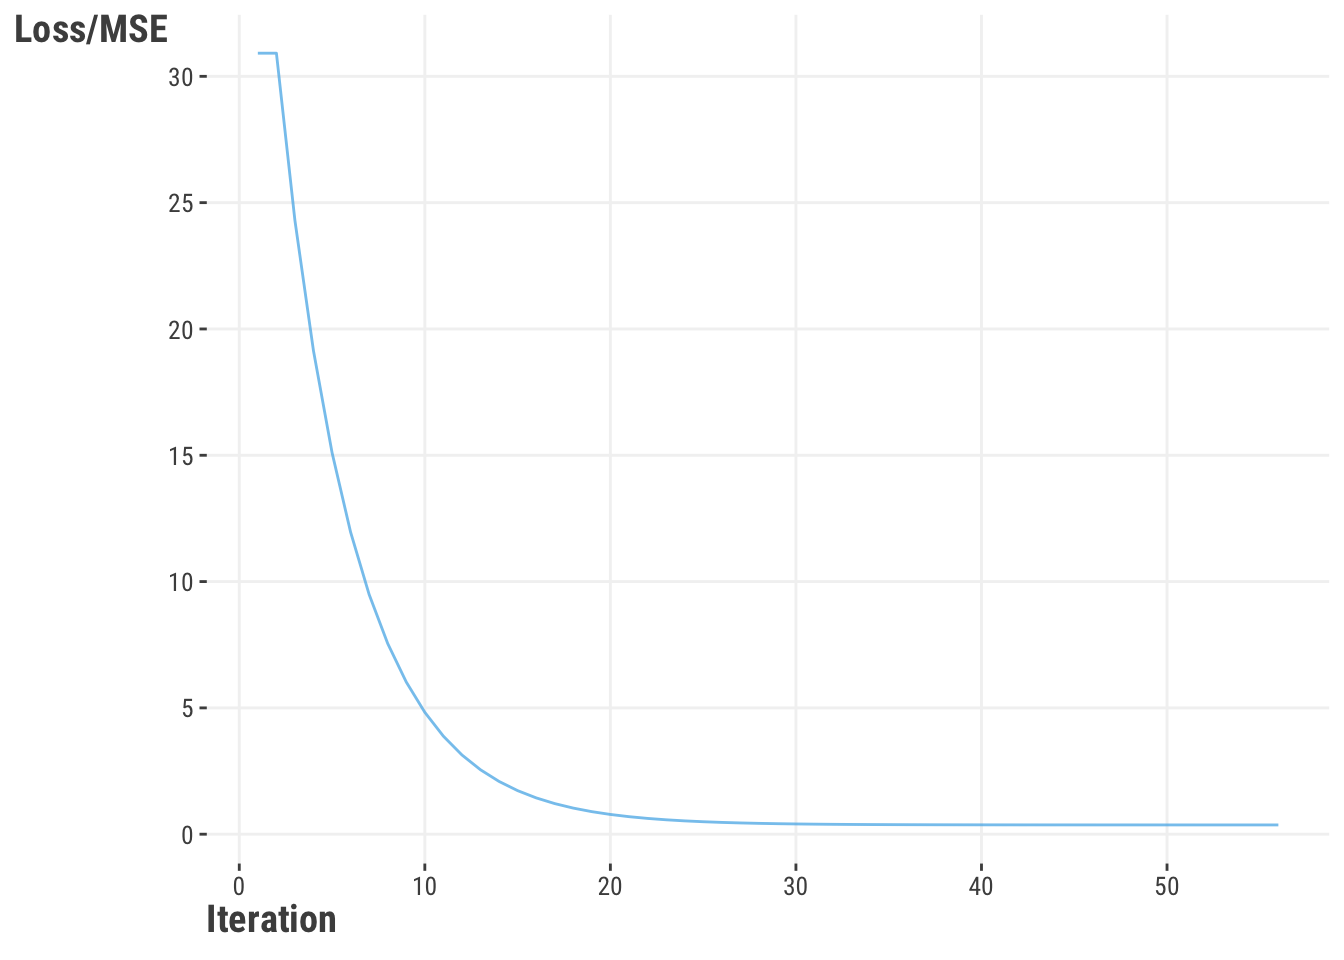
\includegraphics{estimation_files/figure-pdf/fig-r-gradient-descent-1.pdf}

}

\caption{\label{fig-r-gradient-descent}Gradient descent path}

\end{figure}

\subsection{Stochastic Gradient
Descent}\label{stochastic-gradient-descent}

\textbf{Stochastic gradient descent} is a variation on gradient descent
that uses a random sample of the data to estimate the gradient, while
the true gradient is the gradient of the objective function with respect
to all of the data. As such, the stochastic gradient descent is less
accurate than gradient descent. The advantage of stochastic gradient
descent is that it is faster than gradient descent. In practice,
stochastic gradient descent is often used in machine learning
applications where the data is large, and the tradeoff between accuracy
and speed is worth it.

Let's see this in action with the happiness data model we used
previously. The following is a conceptual version of the AdaGrad
approach\footnote{MC does not recall exactly where this origin of this
  function came from except that Murphy's PML book was a key reference.},
which is a variation of stochastic gradient descent that adjusts the
learning rate for each parameter. We will also add a variation that
averages the parameter estimates across iterations, which is a common
approach to improve the performance of stochastic gradient descent, but
by default it is not used, just something you can play with. We are
going to use a `batch size' of one, which is similar to a `streaming' or
`online' version where we update the model with each observation. Since
our data are alphabetically ordered, we'll shuffle the data first. We'll
also use a stepsize\_tau parameter, which is a way to adjust the
learning rate at early iterations. We'll set it to zero for now, but you
can play with it to see how it affects the results. The values for the
learning rate and stepsize\_tau are arbitrary, selected after some
initial playing around, but you can play with them to see how they
affect the results.

NOTE: SHOULD MAYBE CLEAN UP/ALTER TO LESS VERBOSE VERSION

\subsubsection{R}

\begin{Shaded}
\begin{Highlighting}[]
\NormalTok{stochastic\_gradient\_descent }\OtherTok{\textless{}{-}} \ControlFlowTok{function}\NormalTok{(}
\NormalTok{    par, }\CommentTok{\# parameter estimates}
\NormalTok{    X, }\CommentTok{\# model matrix}
\NormalTok{    y, }\CommentTok{\# target variable}
    \AttributeTok{learning\_rate =} \DecValTok{1}\NormalTok{, }\CommentTok{\# the learning rate}
    \AttributeTok{stepsize\_tau =} \DecValTok{0}\NormalTok{, }\CommentTok{\# if \textgreater{} 0, a check on the LR at early iterations}
    \AttributeTok{average =} \ConstantTok{FALSE} \CommentTok{\# a variation of the approach}
\NormalTok{    ) \{}
    \CommentTok{\# initialize}
\NormalTok{    X }\OtherTok{\textless{}{-}} \FunctionTok{cbind}\NormalTok{(}\DecValTok{1}\NormalTok{, X)}
\NormalTok{    beta }\OtherTok{\textless{}{-}}\NormalTok{ par}

    \CommentTok{\# Collect all estimates}
\NormalTok{    betamat }\OtherTok{\textless{}{-}} \FunctionTok{matrix}\NormalTok{(}\DecValTok{0}\NormalTok{, }\FunctionTok{nrow}\NormalTok{(X), }\AttributeTok{ncol =} \FunctionTok{length}\NormalTok{(beta))}

    \CommentTok{\# Collect fitted values at each point))}
\NormalTok{    fits }\OtherTok{\textless{}{-}} \ConstantTok{NA}

    \CommentTok{\# Collect loss at each point}
\NormalTok{    loss }\OtherTok{\textless{}{-}} \ConstantTok{NA}

    \CommentTok{\# adagrad per parameter learning rate adjustment}
\NormalTok{    s }\OtherTok{\textless{}{-}} \DecValTok{0}

    \CommentTok{\# a smoothing term to avoid division by zero}
\NormalTok{    eps }\OtherTok{\textless{}{-}} \FloatTok{1e{-}8}

    \ControlFlowTok{for}\NormalTok{ (i }\ControlFlowTok{in} \DecValTok{1}\SpecialCharTok{:}\FunctionTok{nrow}\NormalTok{(X)) \{}
\NormalTok{        Xi }\OtherTok{\textless{}{-}}\NormalTok{ X[i, , drop }\OtherTok{=} \ConstantTok{FALSE}\NormalTok{]}
\NormalTok{        yi }\OtherTok{\textless{}{-}}\NormalTok{ y[i]}

        \CommentTok{\# matrix operations not necessary here,}
        \CommentTok{\# but makes consistent with standard gd func}
\NormalTok{        LP }\OtherTok{\textless{}{-}}\NormalTok{ Xi }\SpecialCharTok{\%*\%}\NormalTok{ beta}
\NormalTok{        grad }\OtherTok{\textless{}{-}} \FunctionTok{t}\NormalTok{(Xi) }\SpecialCharTok{\%*\%}\NormalTok{ (LP }\SpecialCharTok{{-}}\NormalTok{ yi)}
\NormalTok{        s }\OtherTok{\textless{}{-}}\NormalTok{ s }\SpecialCharTok{+}\NormalTok{ grad}\SpecialCharTok{\^{}}\DecValTok{2} \CommentTok{\# adagrad approach}

        \CommentTok{\# update}
\NormalTok{        beta }\OtherTok{\textless{}{-}}\NormalTok{ beta }\SpecialCharTok{{-}}\NormalTok{ learning\_rate }\SpecialCharTok{/}\NormalTok{ (stepsize\_tau }\SpecialCharTok{+} \FunctionTok{sqrt}\NormalTok{(s }\SpecialCharTok{+}\NormalTok{ eps)) }\SpecialCharTok{*}\NormalTok{ grad}

        \CommentTok{\# a variation}
        \ControlFlowTok{if}\NormalTok{ (average }\SpecialCharTok{\&}\NormalTok{ i }\SpecialCharTok{\textgreater{}} \DecValTok{1}\NormalTok{) \{}
\NormalTok{            beta }\OtherTok{\textless{}{-}}\NormalTok{ beta }\SpecialCharTok{{-}} \DecValTok{1} \SpecialCharTok{/}\NormalTok{ i }\SpecialCharTok{*}\NormalTok{ (betamat[i }\SpecialCharTok{{-}} \DecValTok{1}\NormalTok{, ] }\SpecialCharTok{{-}}\NormalTok{ beta)}
\NormalTok{        \}}

\NormalTok{        betamat[i, ] }\OtherTok{\textless{}{-}}\NormalTok{ beta}
\NormalTok{        fits[i] }\OtherTok{\textless{}{-}}\NormalTok{ LP}
\NormalTok{        loss[i] }\OtherTok{\textless{}{-}} \FunctionTok{crossprod}\NormalTok{(LP }\SpecialCharTok{{-}}\NormalTok{ yi)}
\NormalTok{    \}}

\NormalTok{    LP }\OtherTok{\textless{}{-}}\NormalTok{ X }\SpecialCharTok{\%*\%}\NormalTok{ beta}
\NormalTok{    lastloss }\OtherTok{\textless{}{-}} \FunctionTok{crossprod}\NormalTok{(LP }\SpecialCharTok{{-}}\NormalTok{ y)}

    \FunctionTok{list}\NormalTok{(}
        \AttributeTok{par =}\NormalTok{ beta, }\CommentTok{\# final estimates}
        \AttributeTok{par\_chain =}\NormalTok{ betamat, }\CommentTok{\# estimates at each iteration}
        \AttributeTok{MSE =} \FunctionTok{sum}\NormalTok{(lastloss) }\SpecialCharTok{/} \FunctionTok{nrow}\NormalTok{(X),}
        \AttributeTok{fitted =}\NormalTok{ LP}
\NormalTok{    )}
\NormalTok{\}}

\CommentTok{\# setting a seed ensures replicability}
\FunctionTok{set.seed}\NormalTok{(}\DecValTok{123}\NormalTok{)}

\CommentTok{\# generate random sample indices (could also have done within the function)}
\NormalTok{idx }\OtherTok{\textless{}{-}} \FunctionTok{sample}\NormalTok{(}\DecValTok{1}\SpecialCharTok{:}\FunctionTok{nrow}\NormalTok{(df\_happiness), }\FunctionTok{nrow}\NormalTok{(df\_happiness))}

\NormalTok{X\_train }\OtherTok{=}\NormalTok{ df\_happiness }\SpecialCharTok{|\textgreater{}}
    \FunctionTok{select}\NormalTok{(life\_exp, gdp\_pc, corrupt) }\SpecialCharTok{|\textgreater{}}
\NormalTok{    dplyr}\SpecialCharTok{::}\FunctionTok{slice}\NormalTok{(idx) }\SpecialCharTok{|\textgreater{}}
    \FunctionTok{as.matrix}\NormalTok{()}

\NormalTok{y\_train }\OtherTok{\textless{}{-}}\NormalTok{ df\_happiness}\SpecialCharTok{$}\NormalTok{happiness[idx]}

\NormalTok{our\_result }\OtherTok{\textless{}{-}} \FunctionTok{stochastic\_gradient\_descent}\NormalTok{(}
    \AttributeTok{par =} \FunctionTok{c}\NormalTok{(}\FunctionTok{mean}\NormalTok{(df\_happiness}\SpecialCharTok{$}\NormalTok{happiness), }\DecValTok{0}\NormalTok{, }\DecValTok{0}\NormalTok{, }\DecValTok{0}\NormalTok{),}
    \AttributeTok{X =}\NormalTok{ X\_train,}
    \AttributeTok{y =}\NormalTok{ y\_train,}
    \AttributeTok{learning\_rate =}\NormalTok{ .}\DecValTok{15}\NormalTok{,}
    \AttributeTok{stepsize\_tau =}\NormalTok{ .}\DecValTok{1}
\NormalTok{)}
\end{Highlighting}
\end{Shaded}

\subsubsection{Python}

\begin{Shaded}
\begin{Highlighting}[]
\KeywordTok{def}\NormalTok{ stochastic\_gradient\_descent(}
\NormalTok{    par, }\CommentTok{\# parameter estimates}
\NormalTok{    X, }\CommentTok{\# model matrix}
\NormalTok{    y, }\CommentTok{\# target variable}
\NormalTok{    learning\_rate }\OperatorTok{=} \DecValTok{1}\NormalTok{, }\CommentTok{\# the learning rate}
\NormalTok{    stepsize\_tau }\OperatorTok{=} \DecValTok{0}\NormalTok{, }\CommentTok{\# if \textgreater{} 0, a check on the LR at early iterations}
\NormalTok{    average }\OperatorTok{=} \VariableTok{False} \CommentTok{\# a variation of the approach}
\NormalTok{):}
    \CommentTok{\# initialize}
\NormalTok{    X }\OperatorTok{=}\NormalTok{ np.c\_[np.ones(X.shape[}\DecValTok{0}\NormalTok{]), X]}
\NormalTok{    beta }\OperatorTok{=}\NormalTok{ par}

    \CommentTok{\# Collect all estimates}
\NormalTok{    betamat }\OperatorTok{=}\NormalTok{ np.zeros((X.shape[}\DecValTok{0}\NormalTok{], beta.shape[}\DecValTok{0}\NormalTok{]))}

    \CommentTok{\# Collect fitted values at each point))}
\NormalTok{    fits }\OperatorTok{=}\NormalTok{ np.zeros(X.shape[}\DecValTok{0}\NormalTok{])}

    \CommentTok{\# Collect loss at each point}
\NormalTok{    loss }\OperatorTok{=}\NormalTok{ np.zeros(X.shape[}\DecValTok{0}\NormalTok{])}

    \CommentTok{\# adagrad per parameter learning rate adjustment}
\NormalTok{    s }\OperatorTok{=} \DecValTok{0}

    \CommentTok{\# a smoothing term to avoid division by zero}
\NormalTok{    eps }\OperatorTok{=} \FloatTok{1e{-}8}

    \ControlFlowTok{for}\NormalTok{ i }\KeywordTok{in} \BuiltInTok{range}\NormalTok{(X.shape[}\DecValTok{0}\NormalTok{]):}
\NormalTok{        Xi }\OperatorTok{=}\NormalTok{ X[}\VariableTok{None}\NormalTok{, i, :]}
\NormalTok{        yi }\OperatorTok{=}\NormalTok{ y[i]}

        \CommentTok{\# matrix operations not necessary here,}
        \CommentTok{\# but makes consistent with standard gd func}
\NormalTok{        LP }\OperatorTok{=}\NormalTok{ Xi }\OperatorTok{@}\NormalTok{ beta}
\NormalTok{        grad }\OperatorTok{=}\NormalTok{ Xi.T }\OperatorTok{@}\NormalTok{ (LP }\OperatorTok{{-}}\NormalTok{ yi)}
\NormalTok{        s }\OperatorTok{=}\NormalTok{ s }\OperatorTok{+}\NormalTok{ grad}\OperatorTok{**}\DecValTok{2} \CommentTok{\# adagrad approach}

        \CommentTok{\# update}
\NormalTok{        beta }\OperatorTok{=}\NormalTok{ beta }\OperatorTok{{-}}\NormalTok{ learning\_rate }\OperatorTok{/}\NormalTok{ (stepsize\_tau }\OperatorTok{+}\NormalTok{ np.sqrt(s }\OperatorTok{+}\NormalTok{ eps)) }\OperatorTok{*}\NormalTok{ grad}

        \CommentTok{\# a variation}
        \ControlFlowTok{if}\NormalTok{ (average }\OperatorTok{\&}\NormalTok{ i }\OperatorTok{\textgreater{}} \DecValTok{1}\NormalTok{):}
\NormalTok{            beta }\OperatorTok{=}\NormalTok{ beta }\OperatorTok{{-}} \DecValTok{1} \OperatorTok{/}\NormalTok{ i }\OperatorTok{*}\NormalTok{ (betamat[i }\OperatorTok{{-}} \DecValTok{1}\NormalTok{, :] }\OperatorTok{{-}}\NormalTok{ beta)}

\NormalTok{        betamat[i, :] }\OperatorTok{=}\NormalTok{ beta}
\NormalTok{        fits[i] }\OperatorTok{=}\NormalTok{ LP}
\NormalTok{        loss[i] }\OperatorTok{=}\NormalTok{ np.}\BuiltInTok{sum}\NormalTok{((LP }\OperatorTok{{-}}\NormalTok{ yi)}\OperatorTok{**}\DecValTok{2}\NormalTok{)}

\NormalTok{    LP }\OperatorTok{=}\NormalTok{ X }\OperatorTok{@}\NormalTok{ beta}
\NormalTok{    lastloss }\OperatorTok{=}\NormalTok{ np.}\BuiltInTok{sum}\NormalTok{((LP }\OperatorTok{{-}}\NormalTok{ y)}\OperatorTok{**}\DecValTok{2}\NormalTok{)}

    \ControlFlowTok{return}\NormalTok{(\{}
        \StringTok{"par"}\NormalTok{: beta, }\CommentTok{\# final estimates}
        \StringTok{"par\_chain"}\NormalTok{: betamat, }\CommentTok{\# estimates at each iteration}
        \StringTok{"MSE"}\NormalTok{: lastloss }\OperatorTok{/}\NormalTok{ X.shape[}\DecValTok{0}\NormalTok{],}
        \StringTok{"fitted"}\NormalTok{: LP}
\NormalTok{    \})}

\CommentTok{\# setting a seed ensures replicability}
\NormalTok{np.random.seed(}\DecValTok{1234}\NormalTok{)}

\CommentTok{\# generate random sample indices (could also have done within the function)}
\NormalTok{idx }\OperatorTok{=}\NormalTok{ np.random.choice(df\_happiness.shape[}\DecValTok{0}\NormalTok{], df\_happiness.shape[}\DecValTok{0}\NormalTok{], replace }\OperatorTok{=} \VariableTok{False}\NormalTok{)}

\NormalTok{X\_train }\OperatorTok{=}\NormalTok{ df\_happiness[[}\StringTok{\textquotesingle{}life\_exp\textquotesingle{}}\NormalTok{, }\StringTok{\textquotesingle{}gdp\_pc\textquotesingle{}}\NormalTok{, }\StringTok{\textquotesingle{}corrupt\textquotesingle{}}\NormalTok{]].to\_numpy()[idx, :]}
\NormalTok{y\_train }\OperatorTok{=}\NormalTok{ df\_happiness[}\StringTok{\textquotesingle{}happiness\textquotesingle{}}\NormalTok{].to\_numpy()[idx]}

\NormalTok{our\_result }\OperatorTok{=}\NormalTok{ stochastic\_gradient\_descent(}
\NormalTok{    par }\OperatorTok{=}\NormalTok{ np.array([np.mean(df\_happiness[}\StringTok{\textquotesingle{}happiness\textquotesingle{}}\NormalTok{]), }\DecValTok{0}\NormalTok{, }\DecValTok{0}\NormalTok{, }\DecValTok{0}\NormalTok{]),}
\NormalTok{    X }\OperatorTok{=}\NormalTok{ X\_train,}
\NormalTok{    y }\OperatorTok{=}\NormalTok{ y\_train,}
\NormalTok{    learning\_rate }\OperatorTok{=} \FloatTok{.15}\NormalTok{,}
\NormalTok{    stepsize\_tau }\OperatorTok{=} \FloatTok{.1}
\NormalTok{)}
\end{Highlighting}
\end{Shaded}

Next we'll compare it to OLS estimates. Very similar even though SGD
normally would not be used for such a small dataset.

\hypertarget{tbl-stochastic-gradient-descent}{}
\begin{longtable}{lrr}
\caption{\label{tbl-stochastic-gradient-descent}Comparison of stochastic gradient descent results }\tabularnewline

\toprule
Value & Built-in & Our Result \\ 
\midrule
Intercept & $5.44$ & $5.47$ \\ 
Life Exp. Coef. & $0.52$ & $0.51$ \\ 
GDP\_PC & $0.44$ & $0.39$ \\ 
Corrupt & $-0.11$ & $-0.11$ \\ 
MSE & $0.37$ & $0.37$ \\ 
\bottomrule
\end{longtable}

And here's a plot of the estimates as they moved along the data. For
this plot we don't include the intercept as it's on a notably different
scale. We can see that the estimates are moving around a bit, but they
appear to be converging to a solution.

\begin{figure}

{\centering 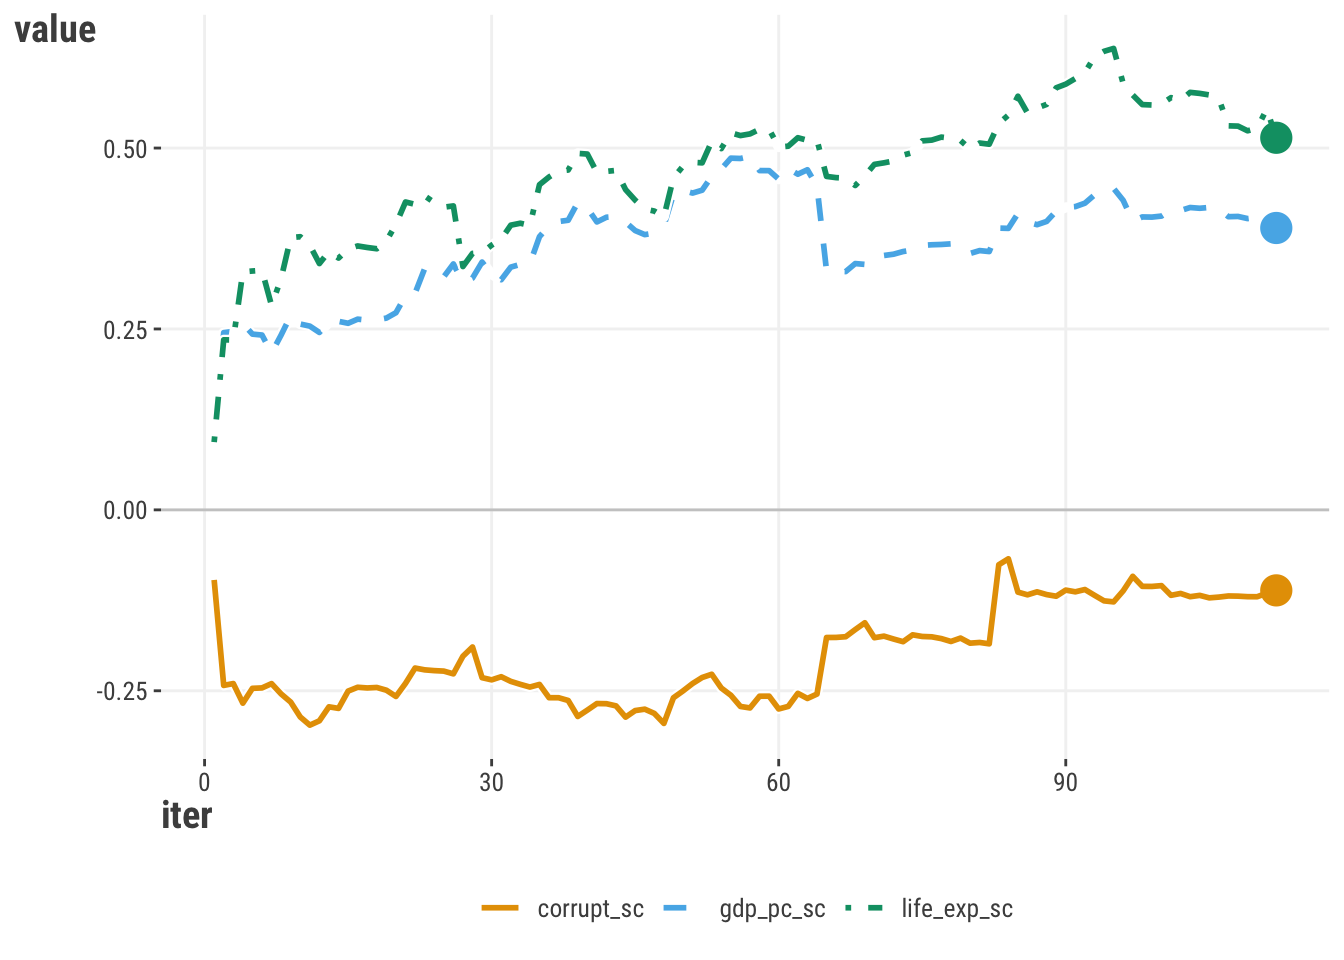
\includegraphics{estimation_files/figure-pdf/fig-r-stochastic-gradient-descent-1.pdf}

}

\caption{\label{fig-r-stochastic-gradient-descent}Stochastic gradient
descent path}

\end{figure}

\subsection{Other Optimization
Algorithms}\label{other-optimization-algorithms}

There are lots of other approaches to optimization. For example, here
are some of the options available in R's \texttt{optim} or scipy's
\texttt{minimize} function:

\begin{itemize}
\tightlist
\item
  Nelder-Mead
\item
  BFGS
\item
  L-BFGS-B (provides constraints)
\item
  Conjugate gradient
\item
  Simulated annealing
\item
  Newton's method
\item
  Genetic algorithms
\end{itemize}

The main reason to choose one method over another usually is some sort
of computational gain, e.g.~memory or speed, or it may just work better
for some types of models in practice. For statistical problems, many
GLM-type functions appear to use Newton's as a default, but more
complicated models may implement other means, and even then might best
be served by a different approach. In general, we can always try a few
different methods to see which works best, and often there would be
little differences in the results. For example, here are the results
from the happiness data using the BFGS method, which is a quasi-Newton
method. Here is our resuls from using OLS, compared to different
algorithms, some we used some we didn't. We can see that the results are
very similar, and for simpler modeling endeavors they should converge on
the same result.

\hypertarget{tbl-optim-compare}{}
\setlength{\LTpost}{0mm}
\begin{longtable}{lrrrrr}
\caption{\label{tbl-optim-compare}Comparison of optimization results }\tabularnewline

\toprule
parameter & NM\textsuperscript{\textit{1}} & BFGS\textsuperscript{\textit{2}} & CG\textsuperscript{\textit{3}} & GD\textsuperscript{\textit{4}} & Built-in \\ 
\midrule
Intercept & $5.445$ & $5.445$ & $5.445$ & $5.437$ & $5.445$ \\ 
Life Exp. Coef. & $0.525$ & $0.525$ & $0.525$ & $0.521$ & $0.525$ \\ 
GDP\_PC & $0.437$ & $0.438$ & $0.438$ & $0.439$ & $0.438$ \\ 
Corrupt & $-0.105$ & $-0.105$ & $-0.105$ & $-0.107$ & $-0.105$ \\ 
MSE & $0.367$ & $0.367$ & $0.367$ & $0.367$ & $0.367$ \\ 
\bottomrule
\end{longtable}
\begin{minipage}{\linewidth}
\textsuperscript{\textit{1}}NM = Nelder-Mead\\
\textsuperscript{\textit{2}}BFGS = Broyden–Fletcher–Goldfarb–Shanno\\
\textsuperscript{\textit{3}}CG = Conjugate gradient\\
\textsuperscript{\textit{4}}GD = Gradient descent\\
\end{minipage}

\section{Other Estimation Approaches}\label{other-estimation-approaches}

Before leaving our estimation discussion, we should mention that there
are many other approaches to estimation that are out there. These
include variaions on least squares, \textbf{method of moments},
\textbf{generalized estimating equations}, \textbf{robust} estimation,
and more. The above that we've focused on will generally be sufficient
for most applications, but it's good to be aware of others. But there
are two we want to discuss in a little bit detail before we leave model
estimation formally given their widespread usage, and that is the
\textbf{bootstrap} and \textbf{Bayesian estimation}.

\subsection{Bootstrap}\label{bootstrap}

The bootstrap is a resampling approach to estimation. We \textbf{sample
with replacement} from the data, generating an entirely new data set of
the same size, and then estimate the model. We repeat this process many
times, collecting parameter estimates, predictions, or any thing we want
to calculate along the way. Ultimately we end up with a distribution of
possible parameter estimates.

This distribution is useful for inference, as we can use the
distribution to calculate confidence intervals, prediction intervals or
intervals for anything we happen to calculate. The average estimate will
typically be the same as whatever the underlying model used would
produced, but the bootstrap provides a way to get at a measure of
uncertainty with fewer assumptions about how that distribution should
take sahape. The bootstrap is very flexible, and it can be used with any
estimation approach. Here is a function to illustrate the process. Let's
see this in action with the happiness data model we used previously.

\subsubsection{R}

\begin{Shaded}
\begin{Highlighting}[]
\NormalTok{bootstrap }\OtherTok{\textless{}{-}} \ControlFlowTok{function}\NormalTok{(X, y, }\AttributeTok{nboot =} \DecValTok{100}\NormalTok{, }\AttributeTok{seed =} \DecValTok{123}\NormalTok{) \{}
    \CommentTok{\# add a column of 1s for the intercept}
\NormalTok{    N }\OtherTok{\textless{}{-}} \FunctionTok{nrow}\NormalTok{(X)}

    \CommentTok{\# initialize}
\NormalTok{    beta }\OtherTok{\textless{}{-}} \FunctionTok{matrix}\NormalTok{(}\ConstantTok{NA}\NormalTok{, (}\DecValTok{1}\SpecialCharTok{+}\FunctionTok{ncol}\NormalTok{(X))}\SpecialCharTok{*}\NormalTok{nboot, }\AttributeTok{nrow =}\NormalTok{ nboot, }\AttributeTok{ncol =} \DecValTok{1}\SpecialCharTok{+}\FunctionTok{ncol}\NormalTok{(X))}
    \FunctionTok{colnames}\NormalTok{(beta) }\OtherTok{\textless{}{-}} \FunctionTok{c}\NormalTok{(}\StringTok{\textquotesingle{}Intercept\textquotesingle{}}\NormalTok{, }\FunctionTok{colnames}\NormalTok{(X))}
\NormalTok{    mse }\OtherTok{\textless{}{-}} \FunctionTok{rep}\NormalTok{(}\ConstantTok{NA}\NormalTok{, nboot)}

    \CommentTok{\# set seed}
    \FunctionTok{set.seed}\NormalTok{(seed)}

    \ControlFlowTok{for}\NormalTok{ (i }\ControlFlowTok{in} \DecValTok{1}\SpecialCharTok{:}\NormalTok{nboot) \{}
        \CommentTok{\# sample with replacement}
\NormalTok{        idx }\OtherTok{\textless{}{-}} \FunctionTok{sample}\NormalTok{(}\DecValTok{1}\SpecialCharTok{:}\NormalTok{N, N, }\AttributeTok{replace =} \ConstantTok{TRUE}\NormalTok{)}
\NormalTok{        Xi }\OtherTok{\textless{}{-}}\NormalTok{ X }\SpecialCharTok{|\textgreater{}} \FunctionTok{slice}\NormalTok{(idx)}
\NormalTok{        yi }\OtherTok{\textless{}{-}}\NormalTok{ y[idx]}

        \CommentTok{\# estimate model}
\NormalTok{        mod }\OtherTok{\textless{}{-}} \FunctionTok{lm}\NormalTok{(yi }\SpecialCharTok{\textasciitilde{}}\NormalTok{., }\AttributeTok{data =}\NormalTok{ Xi)}

        \CommentTok{\# save results}
\NormalTok{        beta[i, ] }\OtherTok{\textless{}{-}} \FunctionTok{coef}\NormalTok{(mod)}
\NormalTok{        mse[i] }\OtherTok{\textless{}{-}} \FunctionTok{sum}\NormalTok{((mod}\SpecialCharTok{$}\NormalTok{fitted }\SpecialCharTok{{-}}\NormalTok{ yi)}\SpecialCharTok{\^{}}\DecValTok{2}\NormalTok{) }\SpecialCharTok{/}\NormalTok{ N}
\NormalTok{    \}}

    \CommentTok{\# given mean estimates, calculate MSE}
\NormalTok{    y\_hat }\OtherTok{=} \FunctionTok{cbind}\NormalTok{(}\DecValTok{1}\NormalTok{, }\FunctionTok{as.matrix}\NormalTok{(X)) }\SpecialCharTok{\%*\%} \FunctionTok{colMeans}\NormalTok{(beta)}
\NormalTok{    final\_mse }\OtherTok{\textless{}{-}} \FunctionTok{sum}\NormalTok{((y }\SpecialCharTok{{-}}\NormalTok{ y\_hat)}\SpecialCharTok{\^{}}\DecValTok{2}\NormalTok{) }\SpecialCharTok{/}\NormalTok{ N}

    \FunctionTok{list}\NormalTok{(}
        \AttributeTok{beta =} \FunctionTok{as\_tibble}\NormalTok{(beta),}
        \AttributeTok{MSE =}\NormalTok{ mse,}
        \AttributeTok{final\_mse =}\NormalTok{ final\_mse}
\NormalTok{    )}
\NormalTok{\}}

\NormalTok{our\_result }\OtherTok{\textless{}{-}} \FunctionTok{bootstrap}\NormalTok{(}
    \AttributeTok{X =}\NormalTok{ df\_happiness }\SpecialCharTok{|\textgreater{}} \FunctionTok{select}\NormalTok{(life\_exp, gdp\_pc, corrupt),}
    \AttributeTok{y =}\NormalTok{ df\_happiness}\SpecialCharTok{$}\NormalTok{happiness,}
    \AttributeTok{nboot =} \DecValTok{250}
\NormalTok{)}
\end{Highlighting}
\end{Shaded}

\subsubsection{Python}

\begin{Shaded}
\begin{Highlighting}[]
\KeywordTok{def}\NormalTok{ bootstrap(X, y, nboot}\OperatorTok{=}\DecValTok{100}\NormalTok{, seed}\OperatorTok{=}\DecValTok{123}\NormalTok{):}
\NormalTok{    cn }\OperatorTok{=}\NormalTok{ X.columns}
    \CommentTok{\# add a column of 1s for the intercept}
\NormalTok{    X }\OperatorTok{=}\NormalTok{ np.c\_[np.ones(X.shape[}\DecValTok{0}\NormalTok{]), X]}
\NormalTok{    N }\OperatorTok{=}\NormalTok{ X.shape[}\DecValTok{0}\NormalTok{]}

    \CommentTok{\# initialize}
\NormalTok{    beta }\OperatorTok{=}\NormalTok{ np.empty((nboot, X.shape[}\DecValTok{1}\NormalTok{]))}
    
    \CommentTok{\# beta = pd.DataFrame(beta, columns=[\textquotesingle{}Intercept\textquotesingle{}] + list(cn))}
\NormalTok{    mse }\OperatorTok{=}\NormalTok{ np.empty(nboot)    }

    \CommentTok{\# set seed}
\NormalTok{    np.random.seed(seed)}

    \ControlFlowTok{for}\NormalTok{ i }\KeywordTok{in} \BuiltInTok{range}\NormalTok{(nboot):}
        \CommentTok{\# sample with replacement}
\NormalTok{        idx }\OperatorTok{=}\NormalTok{ np.random.randint(}\DecValTok{0}\NormalTok{, N, N)}
\NormalTok{        Xi }\OperatorTok{=}\NormalTok{ X[idx, :]}
\NormalTok{        yi }\OperatorTok{=}\NormalTok{ y[idx]}

        \CommentTok{\# estimate model}
\NormalTok{        model }\OperatorTok{=}\NormalTok{ LinearRegression(fit\_intercept}\OperatorTok{=}\VariableTok{False}\NormalTok{)}
\NormalTok{        mod }\OperatorTok{=}\NormalTok{ model.fit(Xi, yi)}

        \CommentTok{\# save results}
\NormalTok{        beta[i, :] }\OperatorTok{=}\NormalTok{ mod.coef\_}
\NormalTok{        mse[i] }\OperatorTok{=}\NormalTok{ np.}\BuiltInTok{sum}\NormalTok{((mod.predict(Xi) }\OperatorTok{{-}}\NormalTok{ yi)}\OperatorTok{**}\DecValTok{2}\NormalTok{) }\OperatorTok{/}\NormalTok{ N}

    \CommentTok{\# given mean estimates, calculate MSE}
\NormalTok{    y\_hat }\OperatorTok{=}\NormalTok{ X }\OperatorTok{@}\NormalTok{ beta.mean(axis}\OperatorTok{=}\DecValTok{0}\NormalTok{)}
\NormalTok{    final\_mse }\OperatorTok{=}\NormalTok{ np.}\BuiltInTok{sum}\NormalTok{((y }\OperatorTok{{-}}\NormalTok{ y\_hat)}\OperatorTok{**}\DecValTok{2}\NormalTok{) }\OperatorTok{/}\NormalTok{ N}

    \ControlFlowTok{return} \BuiltInTok{dict}\NormalTok{(beta }\OperatorTok{=}\NormalTok{ beta, mse }\OperatorTok{=}\NormalTok{ mse, final\_mse }\OperatorTok{=}\NormalTok{ final\_mse)}

\NormalTok{our\_result }\OperatorTok{=}\NormalTok{ bootstrap(}
\NormalTok{    X }\OperatorTok{=}\NormalTok{ df\_happiness[[}\StringTok{\textquotesingle{}life\_exp\textquotesingle{}}\NormalTok{, }\StringTok{\textquotesingle{}gdp\_pc\textquotesingle{}}\NormalTok{, }\StringTok{\textquotesingle{}corrupt\textquotesingle{}}\NormalTok{]],}
\NormalTok{    y }\OperatorTok{=}\NormalTok{ df\_happiness[}\StringTok{\textquotesingle{}happiness\textquotesingle{}}\NormalTok{],}
\NormalTok{    nboot }\OperatorTok{=} \DecValTok{250}
\NormalTok{)}
\end{Highlighting}
\end{Shaded}

Here are the results of the interval estimates for the coefficients. For
each parameter, we have the mean estimate, the lower and upper bounds of
the 95\% confidence interval, and the width of the interval. We can see
that the bootstrap intervals are wider than the OLS intervals, possibly
better capturing the uncertainty in this model based on not too many
observations.

\hypertarget{tbl-bootstrap}{}
\setlength{\LTpost}{0mm}
\begin{longtable}{lrrrrrr}
\caption{\label{tbl-bootstrap}Bootstrap parameter estimates }\tabularnewline

\toprule
Parameter & mean & lower & upper & Lower OLS & Upper OLS & Diff Width\textsuperscript{\textit{1}} \\ 
\midrule
Intercept & $5.44$ & $5.33$ & $5.55$ & $5.33$ & $5.56$ & $0.23$ \\ 
life\_exp & $0.51$ & $0.30$ & $0.70$ & $0.35$ & $0.70$ & $0.35$ \\ 
gdp\_pc & $0.46$ & $0.18$ & $0.76$ & $0.24$ & $0.64$ & $0.40$ \\ 
corrupt & $-0.10$ & $-0.29$ & $0.09$ & $-0.25$ & $0.04$ & $0.28$ \\ 
\bottomrule
\end{longtable}
\begin{minipage}{\linewidth}
\textsuperscript{\textit{1}}Width of bootstrap estimate minus width of OLS estimate\\
\end{minipage}

Let's look at the bootstrap distributions for each coefficient. With
standard statistical estimates, we are assuming a distribution like the
normal, which is a very specific shape. With the bootstrap, we can be
more flexible, thought often it may tend toward the distribution that
would otherwise be assumed. These aren't perfectly symmetrical, but they
suit our needs in that we can extract the lower and upper quantiles to
create an interval estimate.

\begin{figure}

{\centering 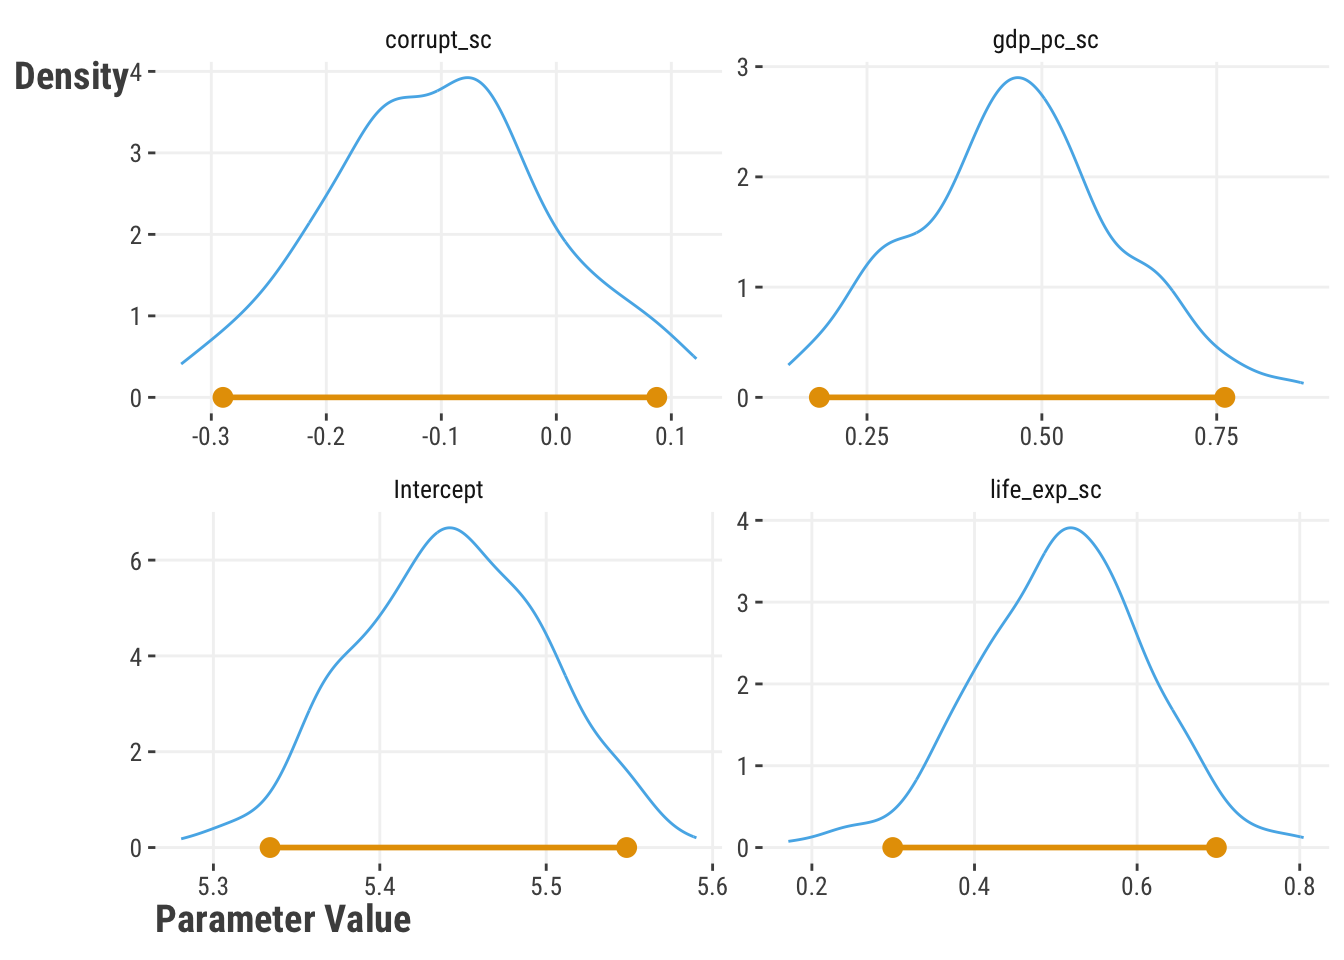
\includegraphics{estimation_files/figure-pdf/fig-r-bootstrap-1.pdf}

}

\caption{\label{fig-r-bootstrap}Bootstrap distributions of parameter
estimates}

\end{figure}

The bootstrap is a commonly used for predictions and other metrics, but
it is computationally inefficient, and can become prohibitive with large
data sizes. Also, the simple bootstrap will likely not estimate the
appropriate uncertainty for some types of statistics (e.g.~extreme
values) or
\href{https://stats.stackexchange.com/questions/9664/what-are-examples-where-a-naive-bootstrap-fails}{in
some data contexts} (e.g.~correlated observations). Overcoming the
limitations may typically require an even more computationally intensive
approach, further limiting its utility. But it is a useful tool to have
in your toolbox, and it can be used in conjunction with other approaches
to get at uncertainty in a model.

\subsection{Bayesian Estimation}\label{bayesian-estimation}

The bayesian approach to modeling is a philosophical view point, an
entirely different way to think about probability, a different way to
measure uncertainty, and on a practical level, just another way to get
model parameter estimates. It can be as frustrating as it is fun to use,
and one of the really nice things about using bayesian estimation is
that it can handle model complexities that other approaches don't do
well.

The basis of bayesian estimation is the \textbf{likelihood}, same as
with maximum likelihood, and everything we did there follows to here.
However, here we can incorporate domain knowledge, in the form of
\textbf{prior distributions} about the parameters, which we specify in
addition to the likelihood. For example, we may say that the
coefficients for a linear model come from a normal distribution centered
on zero with some variance. The combination prior distributions with the
likelihood ultimately results in the \textbf{posterior distribution}.
And this is the key difference when comparing bayesian estimation to the
others we've talked about, and something it shares in common with the
bootstrap- the end result is not a point estimate of the parameters, but
rather a \emph{distribution} of possible parameter values.

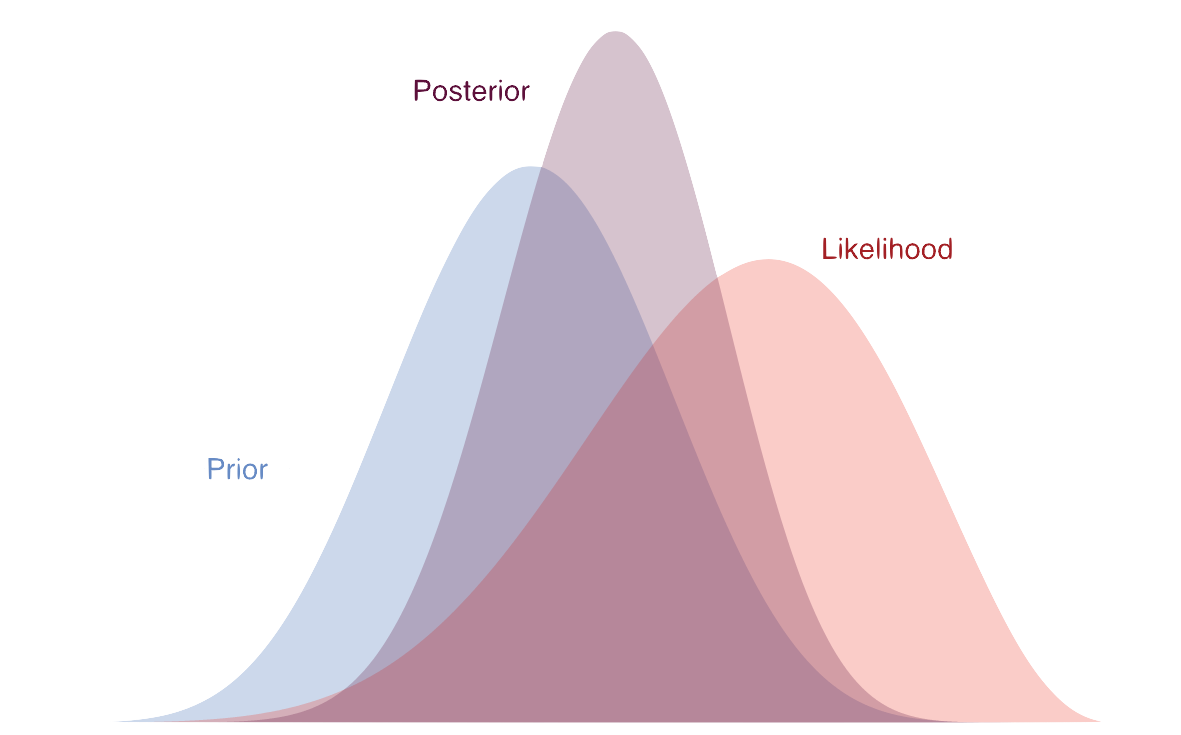
\includegraphics{img/prior2post_clean.png}

Dealing with distributions instead of single estimates is a different
way to think about modeling, but it can be very useful. For example, as
we did with the bootstrap, the bayesian posterior distribution is useful
for inference. With these distributions, we can look at any range in
between for our \textbf{credible interval}, which is the bayesian
equivalent of a confidence interval\footnote{Your default interpretation
  of a standard confidence interval is almost certaintly, and
  incorrectly, the actual interpretation of a Bayesian confidence
  interval, because the Bayesian interpretation of confidence intervals
  and p-values is how we tend to naturally think about them. But that's
  okay, everyone else is in the same boat. We also don't care if you
  want to call the Bayesian version a credible interval or a confidence
  interval.}. Here is an example of the posterior distribution for the
parameters of our happiness model, along with 95\% intervals.

\begin{figure}

{\centering 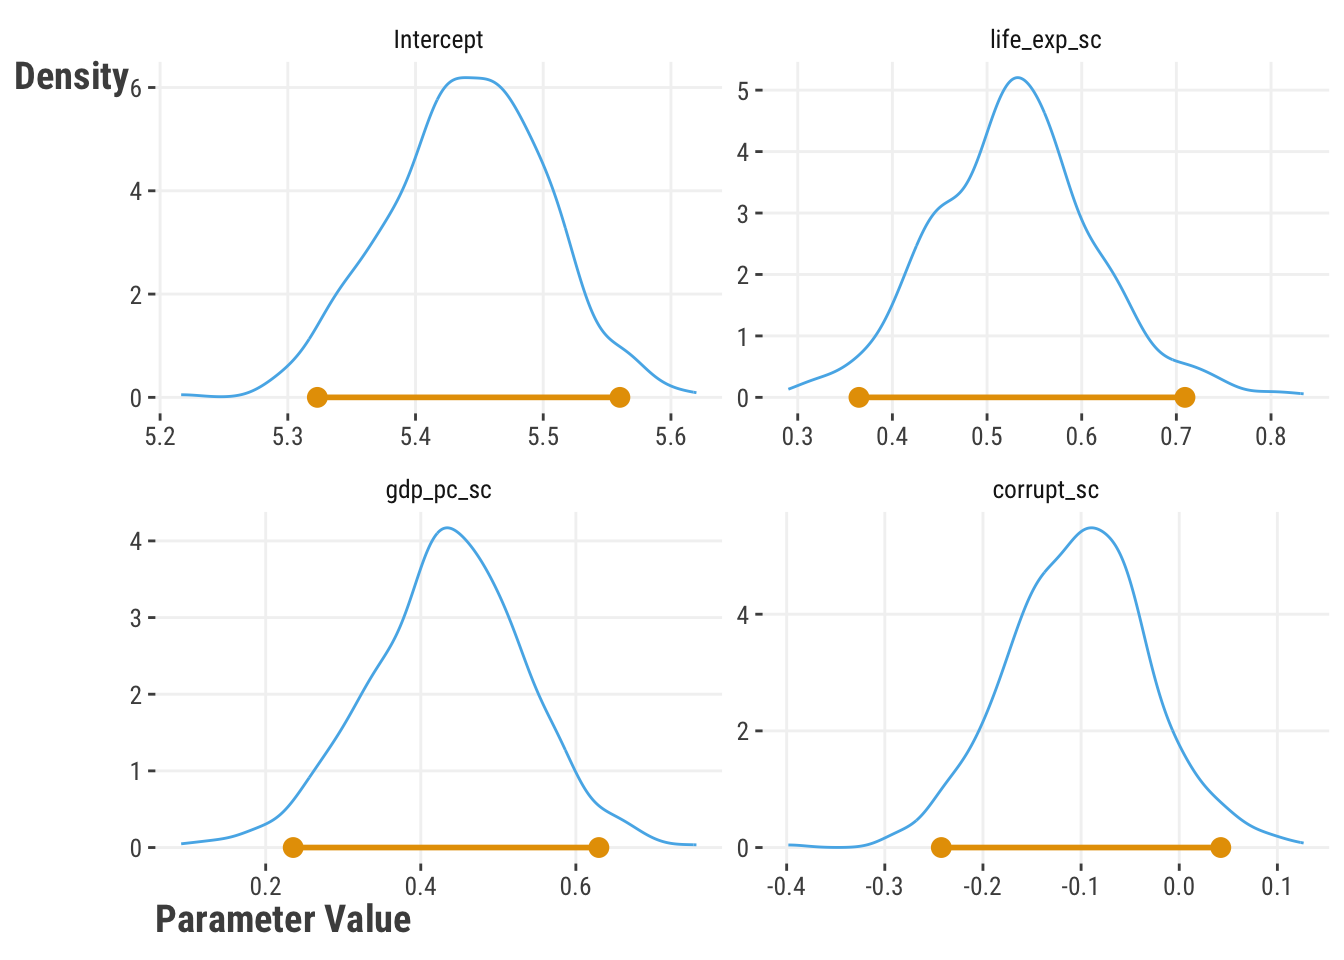
\includegraphics{estimation_files/figure-pdf/fig-r-bayesian-posterior-1.pdf}

}

\caption{\label{fig-r-bayesian-posterior}Posterior distribution of
parameters}

\end{figure}

With bayesian modeling, we use the bayesian algorithm of our choosing,
give it starting values and proceed much in the same way as other
optimization procedures. In the bayesian approach, we always specify a
number of iterations as the \textbf{stopping rule}, i.e.~when the model
should terminate. These iterations are single draws from the posterior
distribution for each parameter. So if we specified 1000 iterations, we
would have 1000 draws from the posterior distribution for each
parameter. Typically we don't use the first few hundred draws, as these
are considered \textbf{burn-in} or \textbf{warmup} draws, and we use the
remaining draws for inference. The number of burn-in draws is a bit of
an art, but it's not too important as long as it's not too small. The
more iterations we set, the longer it will take to run. We also specify
multiple \textbf{chains}, which are each doing the exact same thing, but
do to the random nature of the bayesian approach, would take different
estimation paths. We can then compare the chains to see if they are
converging to the same result, which is a check on the model. If they
are not converging, we may need to run the model longer, or we may need
to change something else. Here is an example of the chains for our
happiness model for the life expectancy coefficient. We can see that
they are converging to the same result, so we are good to go. Nowadays
we have statistics that allow us to check whether the chains are
converging, making it easier to assess many parameters quickly.

\begin{figure}

{\centering 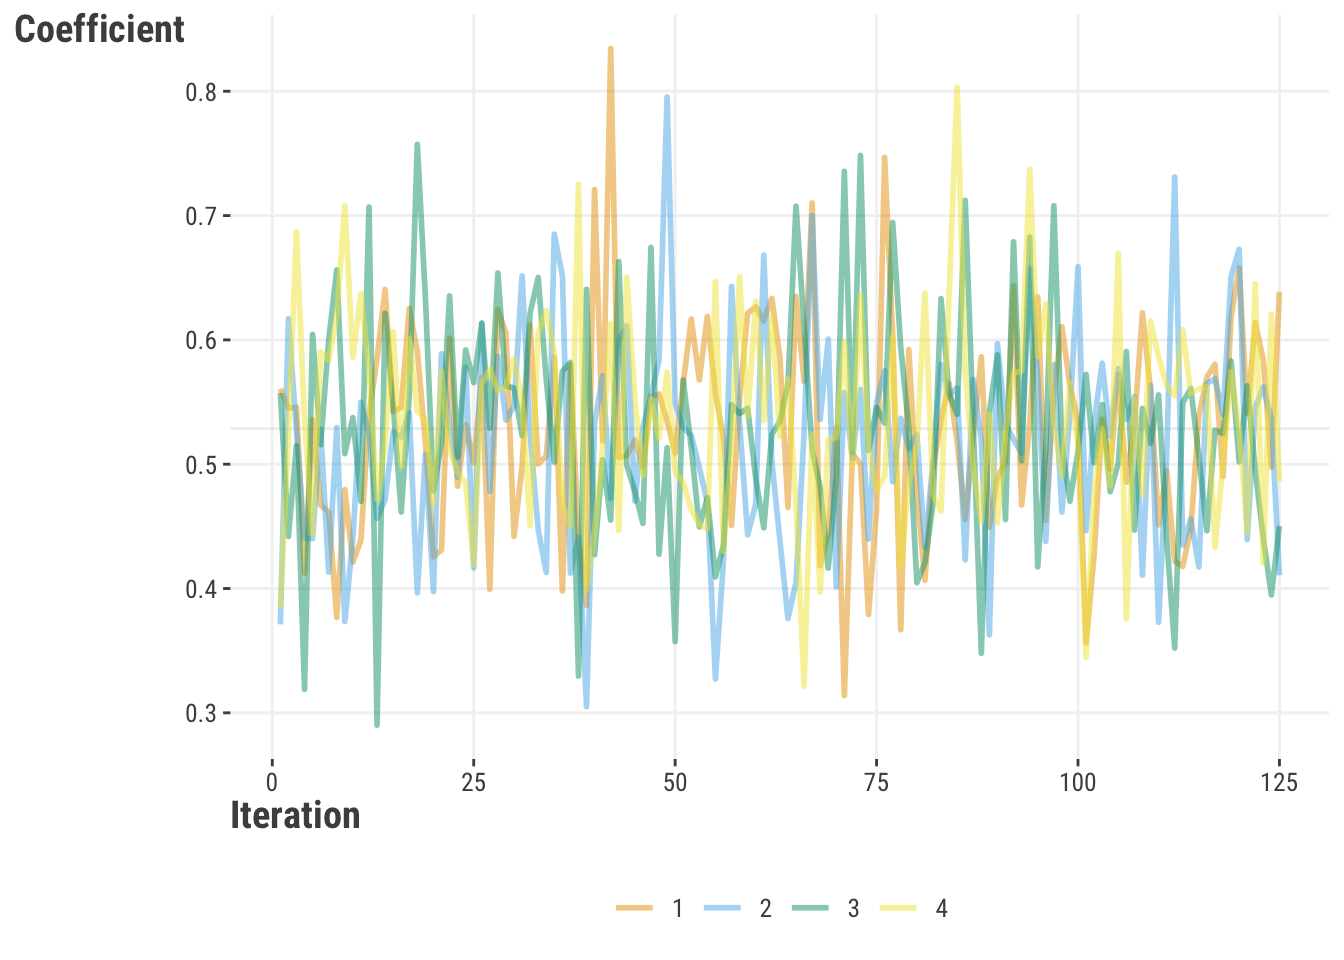
\includegraphics{estimation_files/figure-pdf/fig-r-bayesian-chains-1.pdf}

}

\caption{\label{fig-r-bayesian-chains}Bayesian chains for life
expectancy coefficient}

\end{figure}

When we are interested in making predictions, we can use the results to
generate a distribution of possible predictions \emph{for each
observation}, which can be very useful when we want to quantify
uncertainty in for complex models. This is referred to as
\textbf{posterior predictive distribution}. Here is a plot of several
draws of predicted values against the true happiness scores.

\begin{figure}

{\centering 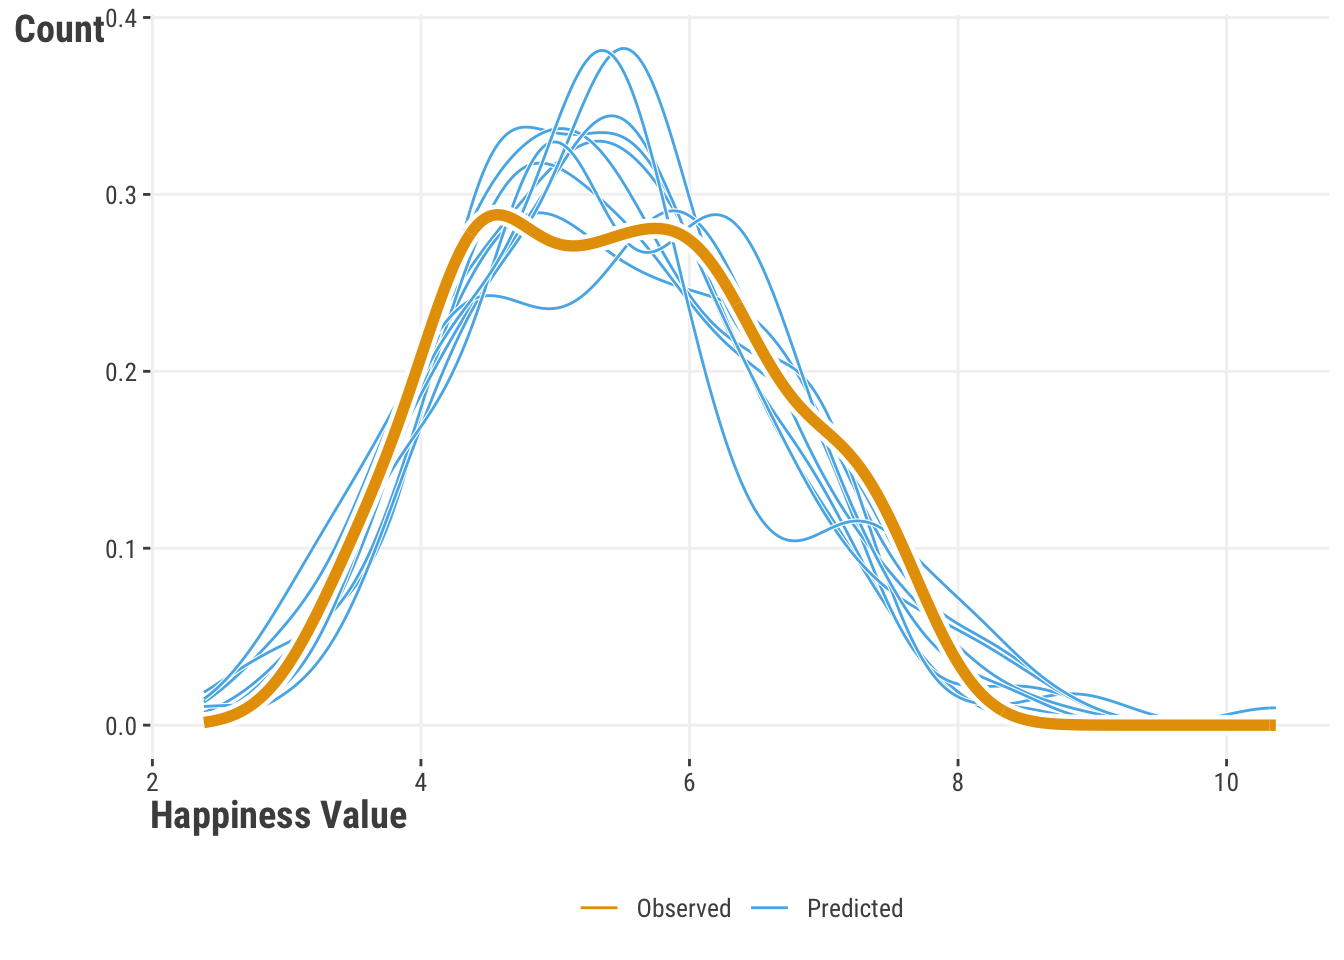
\includegraphics{estimation_files/figure-pdf/fig-r-bayesian-posterior-predictive-1.pdf}

}

\caption{\label{fig-r-bayesian-posterior-predictive}Posterior predictive
distribution of happiness values}

\end{figure}

Note that \emph{any} metric we can calculate from a model will also have
a distribution. For example, you have a classification model and you
want to know the accuracy or true positive rate of the model. Instead of
a single number, you now have access to a distribution of values for
that metric. Why? For every sample of the distribution of parameters,
you generate a prediction, convert it a class and compare it to the true
class. So now you have a posterior predictive distribution for the
predicted probabilities and class, and you can then calculate the
accuracy, area under a receiver operating curve, true positive rate,
etc., for each sample, and you have a distribution of possible values.
As an example, we did this for our happiness model and show the interval
estimate for R\textsuperscript{2}. Pretty neat!

\hypertarget{tbl-r-bayesian-metrics}{}
\setlength{\LTpost}{0mm}
\begin{longtable}{rrr}
\caption{\label{tbl-r-bayesian-metrics}Bayesian R\textsuperscript{2} }\tabularnewline

\toprule
Bayes R2 & Lower & Upper \\ 
\midrule
$0.71$ & $0.65$ & $0.75$ \\ 
\bottomrule
\end{longtable}
\begin{minipage}{\linewidth}
95\% Credible interval for R-squared\\
\end{minipage}

\begin{tcolorbox}[enhanced jigsaw, rightrule=.15mm, opacityback=0, left=2mm, bottomrule=.15mm, toprule=.15mm, arc=.35mm, colframe=quarto-callout-tip-color-frame, leftrule=.75mm, breakable, colback=white]
\begin{minipage}[t]{5.5mm}
\textcolor{quarto-callout-tip-color}{\faLightbulb}
\end{minipage}%
\begin{minipage}[t]{\textwidth - 5.5mm}

There is nothing keeping you from doing posterior predictive checks with
other estimation approaches, and it's a good idea to do so. For example,
in a GLM you have the beta estimates and the covariance matrix for them,
and can simulate from a normal distribution with those estimates. But
it's a bit more straightforward with the bayesian approach, and some
pacakges will allow you to do this automatically even.

\end{minipage}%
\end{tcolorbox}

\subsubsection{Additional Thoughts}\label{additional-thoughts}

It turns out that any standard (frequentist) statistical model can be
seen as a bayesian one from a particular point of view. Here are a
couple:

\begin{itemize}
\tightlist
\item
  GLM and related estimated via maximum likelihood: Bayesian estimation
  with a flat/uniform prior on the parameters.
\item
  Ridge Regression: Bayesian estimation with a normal prior on the
  coefficients, penalty parameter is related to the variance of the
  prior
\item
  Lasso Regression: Bayesian estimation with a Laplace prior on the
  coefficients, penalty parameter is related to the variance of the
  prior
\end{itemize}

So in many modeling contexts, you're probably doing a restrictive form
of bayesian estimation already. Hopefully this helps to demystify the
bayesian approach a bit, and you feel more comfortable switching to it.
R has excellent tools here, like brms and tidybayes, and Python has
pymc3 and arviz, which are also useful.

We can see that the bayesian approach is very flexible, and can be used
for many different types of models, and can be used to get at
uncertainty in a model in ways that other approaches can't. It's not a
panacea, and it's not always the best approach, but it's a good one to
have in your toolbox.

WHERE TO PUT THIS PRIOR STUFF?

The tough part about the bayesian approach is specifying priors, but
even when you don't have a great idea, many have offered solutions, and
there are ways to check whether what you've chosen makes sense for your
data before trying the model itself.

\begin{tcolorbox}[enhanced jigsaw, rightrule=.15mm, opacityback=0, left=2mm, bottomrule=.15mm, toprule=.15mm, arc=.35mm, colframe=quarto-callout-tip-color-frame, leftrule=.75mm, breakable, colback=white]
\begin{minipage}[t]{5.5mm}
\textcolor{quarto-callout-tip-color}{\faLightbulb}
\end{minipage}%
\begin{minipage}[t]{\textwidth - 5.5mm}

Specification of priors can be done in different ways, and nowadays,
there is a lot of information on how to do so, and with some tools, it's
also pretty straightforward to check whether the priors are sensible
without even running a model. When you do have actual prior knowledge,
either domain knowledge (e.g.~a prior study found the beta values to be
positive), statistical knowledge, (e.g.~only the largest standard
coefficients go near or beyond 1), data from time periods, there's
typically at least something to help you specify your priors with
sensible values. This takes away most of the luster of the primary
argument against the bayesian approach, which is the subjective nature
of priors. But there is likewise so much subjective decision making in
other approaches, that it's not really a useful argument to begin with.
The bayesian approach just makes it more explicit. And if you don't have
any prior knowledge, you can use non- or weakly- informative priors,
which will likely have little influence and let the data do the talking,
producing a result that is not that different from maximum likelihood
estimation.

\end{minipage}%
\end{tcolorbox}

MOVE MH EXAMPLE TO APPENDIX

Metropolis-Hastings demo

\section{Commentary}\label{commentary-2}

\section{Refs}\label{refs}

Maximum Likelihood

SGD

\href{https://www.youtube.com/watch?v=sDv4f4s2SB8}{Gradient Descent,
Step-by-Step}
\href{https://www.youtube.com/watch?v=vMh0zPT0tLI}{Stochastic Gradient
Descent, Clearly Explained!!!}
https://www.databricks.com/glossary/adagrad
https://machinelearningmastery.com/gradient-descent-with-adagrad-from-scratch/

Bayesian

\begin{itemize}
\tightlist
\item
  BDA
\item
  Statistical Rethinking
\item
  \href{https://github.com/stan-dev/stan/wiki/Prior-Choice-Recommendations}{Prior
  Specification}
\end{itemize}

\chapter{Generalized Linear Models}\label{generalized-linear-models}

What happens when your target variable isn't really a continuous
variable, but is instead some other type of response. Maybe you've got a
binary condition, like good or bad, or maybe you've got a count of
something, like the number of times a person has been arrested. In these
cases, you can't use a linear regression, but you can use a generalized
linear model.

Generalized linear models exist to map different distributions into
linear space. This allows us to use the same linear model framework that
we've been using, but with different types of data.

These models work by \textbf{generalizing} the linear model to different
distributions of the target variable. Our coefficients will certainly
take on a new meaning; so while we cannot interpret them as we would
coefficients from a linear regression, we can still use the general
framework.

\section{Distributions \& Link
Functions}\label{distributions-link-functions}

Remember how linear models really enjoy the whole Gaussian distribution
scene? The essential form of the linear model can be expressed as
follows:

\[y \sim Normal(\mu,\sigma) \\ \mu = \alpha + \beta X\]

Not all data follows a Gaussian distribution. Instead, we often find
some other form of an exponential distribution. So, we need a way to
incorporate different distributions of the target into our model.
Distributions cannot do it alone! We also need a \textbf{link function}
to connect the linear model to the distribution.

From a theoretical perspective, link functions are tricky to get your
head around.

\begin{itemize}
\tightlist
\item
  \emph{Find the exponential of the response's density function and
  derive the canonical link function}\ldots{}
\end{itemize}

From a conceptual perspective, all they are doing is allowing the linear
feature to ``link'' to a distribution function's mean. If you know a
distribution's canonical link function, that is all the deeper you will
probably every need.

At the end of the day, these link functions will convert the target to
an unbounded continuous variable. The take-away here is that the link
function describes how the mean is generated from the predictors.

\section{Logistic Regression}\label{logistic-regression}

\subsection{Why Should You Care}\label{why-should-you-care}

You will often have a binary variable that you might want to use as a
target -- it could be dead/alive, lose/win, quit/retain, etc. You might
be tempted to use a linear regression, but you will quickly find that it
is not the best option. You are going to be figuring out the probability
of moving from ``failure'' to ``success'', given the features in your
model.

\subsection{The Binomial Distribution}\label{the-binomial-distribution}

Logistic regression is substantially different than linear regression.
It is also a bit confusing, because it is named after its link function
(\textbf{logit}) instead of its distribution (\textbf{binomial}).
Instead of that nice continuous target, we are dealing with a
binomially-distributed target and the target takes the form of a binary
variable.

We don't have a \(\mu\) or \(\sigma^2\) to identify the shape of the
binomial distribution; instead we have \emph{p} and \emph{n}, where
\emph{p} is a probability and \emph{n} is the number of trials. We tend
to talk about \emph{p} with regard to the probability of a specific
event happening (heads, wins, defaulting, etc.).

Let's see how the binomial distribution looks with 100 trials and
probabilities of ``success'' at \emph{p = } .25, .5, and .75:

\begin{figure}

{\centering 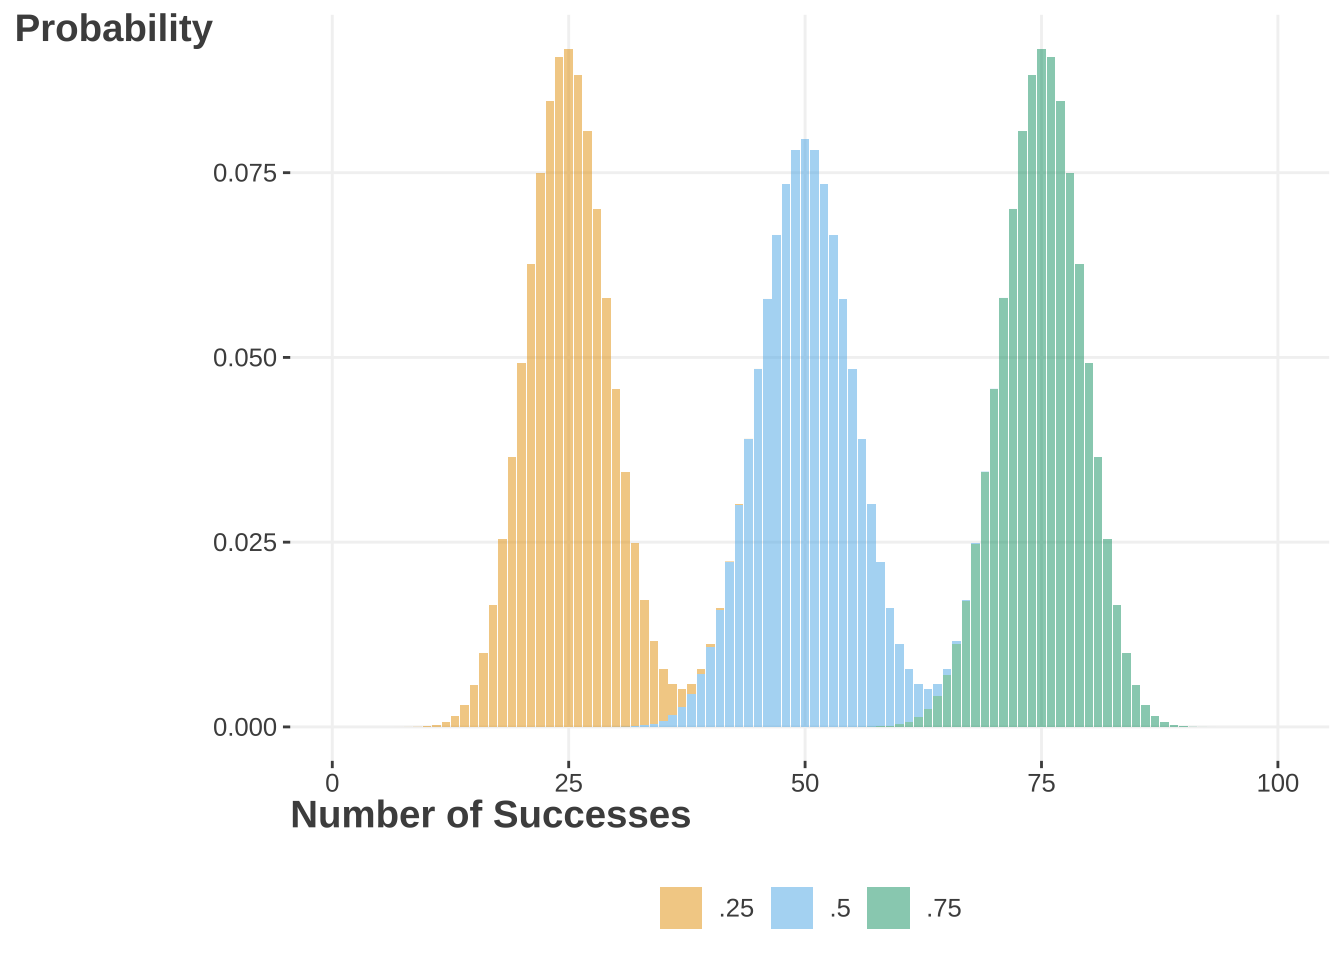
\includegraphics{generalized_linear_models_files/figure-pdf/fig-binomial-1.pdf}

}

\caption{\label{fig-binomial}Binomial distributions for different
probabilities}

\end{figure}

If we examine the distribution for a probability of .5 in
Figure~\ref{fig-binomial}, we will see that it is centered over 50 --
this would suggest that we have the highest probability of encountering
50 successes if we ran 100 trials. If we run 100 trials 100 times and
the outcome is 50/50, the most common outcome from those 100 trials
would be 50 successes. with a decreasing probability of observing more
or less successes as we move away from 50. Shifting our attention to a
.75 probability of success, we see that our density is sitting over 75.
Again running 100 trials, would give us the highest probability of
observing 75 successes. Some of those 100 trials produce more or less
than 75 successes, but with lower probabilities as you get further away
from 75.

Since we are dealing with a number of trials, it is worth noting that
the binomial distribution is a discrete distribution. If you have any
interest in knowing the probability for a number of success under the
binomial distribution, we can use the following formula:

\[P(x) = \frac{n!}{(n-x)!x!}p^xq^{n-x}\]

While we don't need to dive into finding those specific values for the
binomial distribution, we can spend our time exploring how it looks in
linear model space:

\[y \sim Binomial(n, p) \\ logit(p) = \alpha + \beta X\]

The \emph{logit} function is defined as:

\[log\frac{p}{1-p}\]

We are literally just taking the log of the odds (the log odds becomes
important later).

Now we can map this back to our model:

\[log\frac{p}{1-p} = \alpha + \beta X\]

And finally we can take that logistic function and invert it (the
\textbf{inverse-logit}) to produce the probabilities.

\[p = \frac{exp(\alpha + \beta X)}{1 + exp(\alpha + \beta X)}\]

Whenever we get coefficients for the logistic regression model, we are
always going to get them as log odds. We can exponentiate them to get
the odds ratio, but we can also exponentiate them and divide by 1 + that
value to get the probability.

\subsection{Probability, Odds, and Log
Odds}\label{probability-odds-and-log-odds}

Probability lies at the heart of all of this. We can look at the
relationship between the probability, odds, and log odds. We can start
with a set of probability values where \(0 < p > 1\)

With that list of probability values, we can convert them to odds with
\(\\p\, / 1 - p\).

\begin{figure}

{\centering 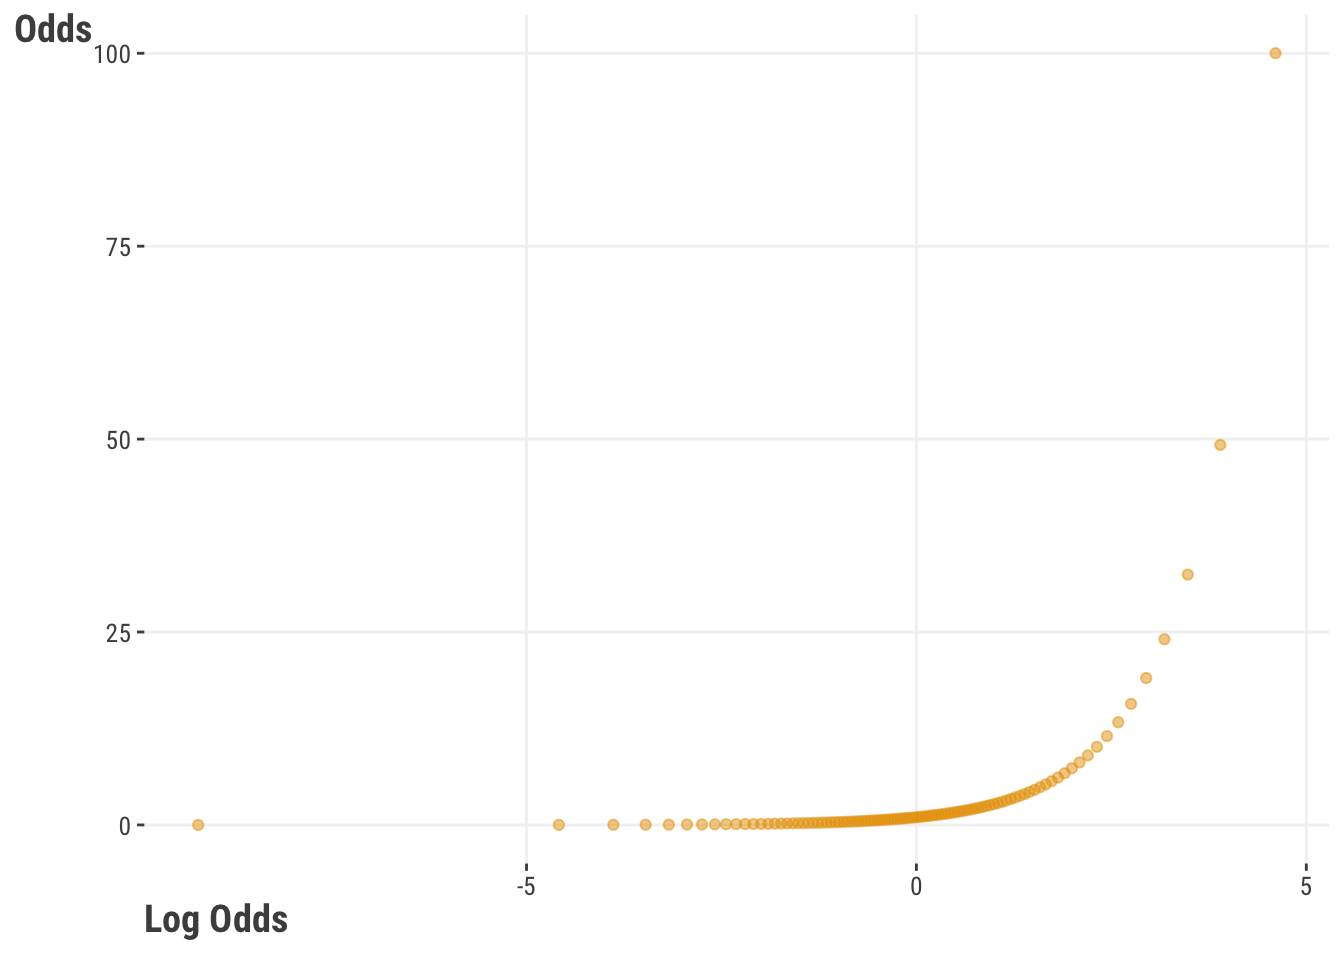
\includegraphics{generalized_linear_models_files/figure-pdf/fig-odds-log-odds-1.pdf}

}

\caption{\label{fig-odds-log-odds}Log odds and odds values for a range
of probabilities}

\end{figure}

We can see how those probability values map to odds in
Figure~\ref{fig-odds-log-odds}.

Now, we can take those odds values and convert them to log odds.

\begin{figure}

{\centering 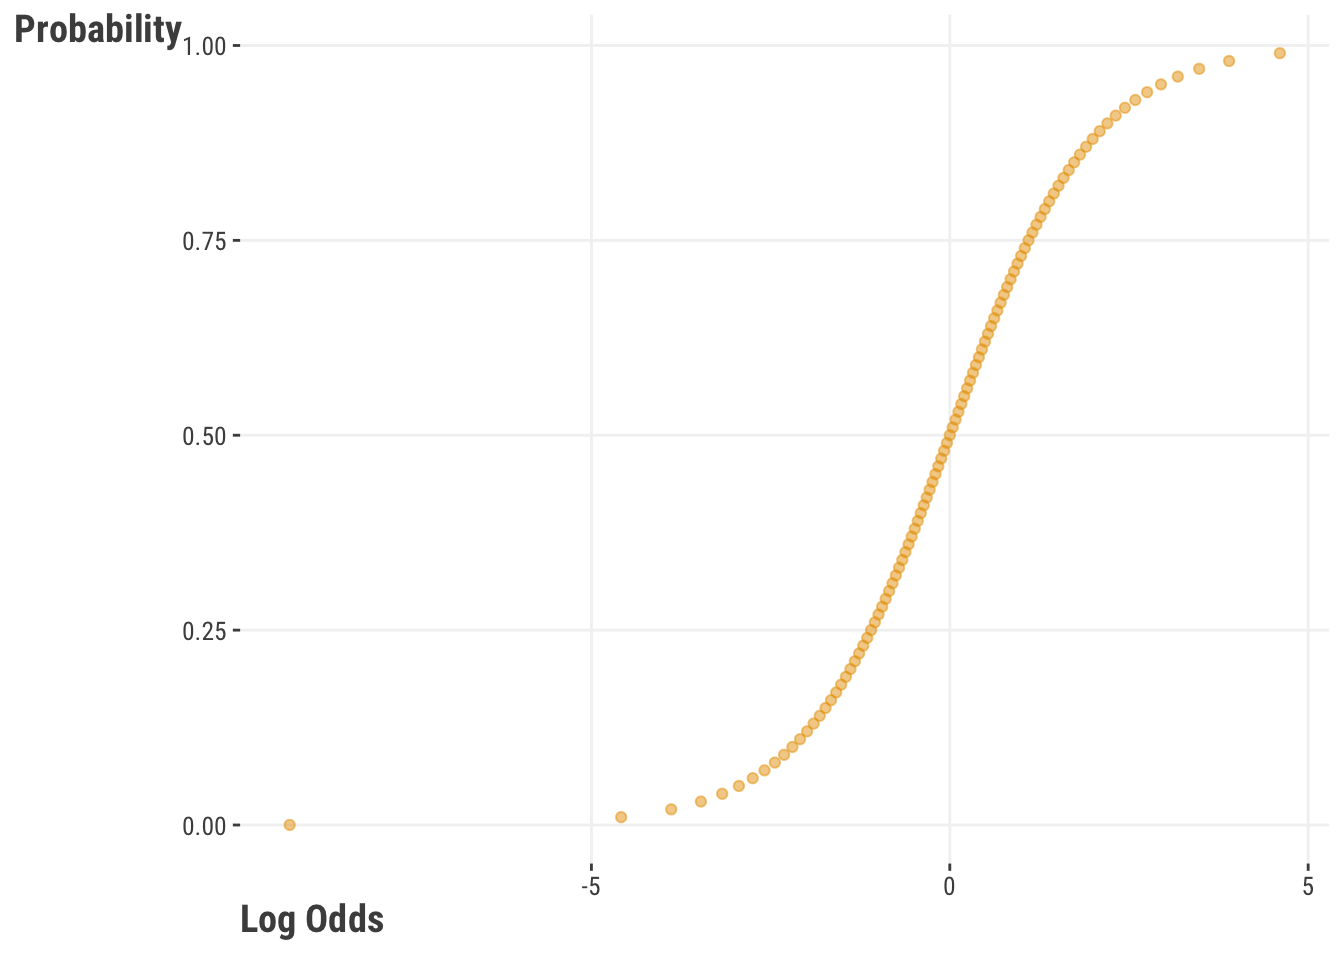
\includegraphics{generalized_linear_models_files/figure-pdf/fig-prob-log-odds-1.pdf}

}

\caption{\label{fig-prob-log-odds}Log odds and probability values}

\end{figure}

If you've ever seen the sigmoid featured in
Figure~\ref{fig-prob-log-odds} before, it is the classic logistic
function!

We can clearly go back and forth between the 3, but the main message
here is that we took a bounded variable in probability and transformed
it to continuous space.

We will see more about how this happens after playing with the model.

\subsection{Data Import and
Preparation}\label{data-import-and-preparation}

We are going to return to our movie reviews data and we are going to use
\texttt{rating\_good} as our target. Before we get to modeling, see if
you can find out the frequency of ``good'' and ``bad'' reviews. We will
use \texttt{word\_count} and \texttt{gender} as our predictors. Before
we move on, though, find the probability of getting a ``good'' review.

\subsubsection{R}

\begin{Shaded}
\begin{Highlighting}[]
\NormalTok{reviews }\OtherTok{\textless{}{-}} \FunctionTok{read.csv}\NormalTok{(}\StringTok{"data/movie\_reviews\_processed.csv"}\NormalTok{)}
\end{Highlighting}
\end{Shaded}

\begin{Shaded}
\begin{Highlighting}[]
\NormalTok{X }\OtherTok{\textless{}{-}}\NormalTok{ reviews[, }\FunctionTok{c}\NormalTok{(}\StringTok{"word\_count"}\NormalTok{, }\StringTok{"gender"}\NormalTok{)]}

\NormalTok{X }\OtherTok{=} \FunctionTok{cbind}\NormalTok{(}\DecValTok{1}\NormalTok{, X)}

\NormalTok{X}\SpecialCharTok{$}\NormalTok{gender }\OtherTok{\textless{}{-}} \FunctionTok{ifelse}\NormalTok{(X}\SpecialCharTok{$}\NormalTok{gender }\SpecialCharTok{==} \StringTok{"male"}\NormalTok{, }\DecValTok{1}\NormalTok{, }\DecValTok{0}\NormalTok{)}

\NormalTok{X }\OtherTok{\textless{}{-}} \FunctionTok{as.matrix}\NormalTok{(X)}

\NormalTok{y }\OtherTok{\textless{}{-}}\NormalTok{ reviews}\SpecialCharTok{$}\NormalTok{rating\_good}
\end{Highlighting}
\end{Shaded}

\subsubsection{Python}

\begin{Shaded}
\begin{Highlighting}[]
\ImportTok{import}\NormalTok{ pandas }\ImportTok{as}\NormalTok{ pd}

\NormalTok{reviews }\OperatorTok{=}\NormalTok{ pd.read\_csv(}\StringTok{"data/movie\_reviews\_processed.csv"}\NormalTok{)}
\end{Highlighting}
\end{Shaded}

\begin{Shaded}
\begin{Highlighting}[]
\NormalTok{X }\OperatorTok{=}\NormalTok{ reviews[[}\StringTok{\textquotesingle{}word\_count\textquotesingle{}}\NormalTok{, }\StringTok{\textquotesingle{}gender\textquotesingle{}}\NormalTok{]]}

\NormalTok{y }\OperatorTok{=}\NormalTok{ reviews[}\StringTok{"rating\_good"}\NormalTok{]}
\end{Highlighting}
\end{Shaded}

\subsection{Standard Functions}\label{standard-functions}

To get started with our first logistic regression model, let's use the
\texttt{glm} function from R and Python's \texttt{statsmodels} function.

\subsubsection{R}

\begin{Shaded}
\begin{Highlighting}[]
\NormalTok{logistic\_regression }\OtherTok{\textless{}{-}} \FunctionTok{glm}\NormalTok{(}
\NormalTok{    rating\_good }\SpecialCharTok{\textasciitilde{}}\NormalTok{ word\_count }\SpecialCharTok{+}\NormalTok{ gender, }
    \AttributeTok{data =}\NormalTok{ reviews,}
    \AttributeTok{family =}\NormalTok{ binomial}
\NormalTok{)}

\FunctionTok{summary}\NormalTok{(logistic\_regression)}
\end{Highlighting}
\end{Shaded}

\begin{verbatim}

Call:
glm(formula = rating_good ~ word_count + gender, family = binomial, 
    data = reviews)

Coefficients:
            Estimate Std. Error z value Pr(>|z|)    
(Intercept)  1.71240    0.18136   9.442   <2e-16 ***
word_count  -0.14639    0.01551  -9.436   <2e-16 ***
gendermale   0.11891    0.13751   0.865    0.387    
---
Signif. codes:  0 '***' 0.001 '**' 0.01 '*' 0.05 '.' 0.1 ' ' 1

(Dispersion parameter for binomial family taken to be 1)

    Null deviance: 1370.4  on 999  degrees of freedom
Residual deviance: 1257.4  on 997  degrees of freedom
AIC: 1263.4

Number of Fisher Scoring iterations: 4
\end{verbatim}

\subsubsection{Python}

\begin{Shaded}
\begin{Highlighting}[]
\ImportTok{import}\NormalTok{ statsmodels.api }\ImportTok{as}\NormalTok{ sm}

\NormalTok{X }\OperatorTok{=}\NormalTok{ sm.add\_constant(X)}

\NormalTok{X }\OperatorTok{=}\NormalTok{ pd.get\_dummies(X, drop\_first }\OperatorTok{=} \VariableTok{True}\NormalTok{)}

\NormalTok{logistic\_regression }\OperatorTok{=}\NormalTok{ sm.Logit(y, X.astype(}\BuiltInTok{float}\NormalTok{)).fit()}
\end{Highlighting}
\end{Shaded}

\begin{verbatim}
Optimization terminated successfully.
         Current function value: 0.628697
         Iterations 5
\end{verbatim}

\begin{Shaded}
\begin{Highlighting}[]
\NormalTok{logistic\_regression.summary()}
\end{Highlighting}
\end{Shaded}

\begin{verbatim}
<class 'statsmodels.iolib.summary.Summary'>
"""
                           Logit Regression Results                           
==============================================================================
Dep. Variable:            rating_good   No. Observations:                 1000
Model:                          Logit   Df Residuals:                      997
Method:                           MLE   Df Model:                            2
Date:                Sat, 09 Dec 2023   Pseudo R-squ.:                 0.08245
Time:                        10:21:13   Log-Likelihood:                -628.70
converged:                       True   LL-Null:                       -685.19
Covariance Type:            nonrobust   LLR p-value:                 2.925e-25
===============================================================================
                  coef    std err          z      P>|z|      [0.025      0.975]
-------------------------------------------------------------------------------
const           1.7124      0.181      9.442      0.000       1.357       2.068
word_count     -0.1464      0.016     -9.436      0.000      -0.177      -0.116
gender_male     0.1189      0.138      0.865      0.387      -0.151       0.388
===============================================================================
"""
\end{verbatim}

\subsection{Interpretation and
Visualization}\label{interpretation-and-visualization}

We need to know what those results mean. The coefficients that we get
from our model are in log odds. We can exponentiate them to get the odds
ratio, but we can also exponentiate them and divide by 1 + that value to
get the probability. Interpretting log odds is a fool's errand, but we
can at least get a feeling for them directionally. A log odds of 0 would
indicate no relationship between the feature and target. A positive log
odds would indicate that an increase in the feature will increase the
log odds of moving from ``bad'' to ``good'', whereas a negative log odds
would indicate that a decrease in the feature will decrease the log odds
of moving from ``bad'' to ``good''. We can convert those log odds to
help make some more sense from them.

When we exponentiate the log odds coefficients, we are given the odds
ratio. This is the ratio of the odds of the outcome (i.e., success from
our binomial distribution) occurring for a one unit increase in the
predictor.

\begin{verbatim}
(Intercept)  word_count  gendermale 
  5.5422663   0.8638229   1.1262687 
\end{verbatim}

Fortunately, the intercept is easy -- it is the odds of a ``good''
review when word count is 0 and gender is ``female''. We see that we've
got an odds ratio of .86 for the word\_count variable and 1.12 for the
male variable. An odds ratio of 1 means that there is no change in the
odds of the outcome occurring -- essentially that the predictor does not
influence the target. An odds ratio of less than 1 means that the odds
of the outcome occurring decrease as the predictor increases (while a
bit more complicated to wrap your head around, it captures the idea of
the odds of moving from a ``bad'' review to a ``good'' review
decreasing). An odds ratio of greater than 1 means that the odds of the
outcome occurring increase as the predictor increases (again, the odds
of moving from a ``bad'' review to a ``good'' review increasing).

It is far more intuitive to interpret the probability. We can do this by
exponentiating the coefficients and dividing by 1 + that value. This
will give us the probability of the outcome occurring for a one unit
increase in the predictor.

\begin{verbatim}
(Intercept)  word_count  gendermale 
  0.8471478   0.4634683   0.5296925 
\end{verbatim}

We would say that our probability of moving from a ``bad'' review to a
``good'' review is .84 when there are 0 words in the review and the
gender is female. Since word\_count is below .5, we know that it will
have a negative relationship with the probability of moving from ``bad''
to ``good''; being a male reviewer will have a positive relationship
with the probability of moving from ``bad'' to ``good''.

And visualizing those probabilities is absolutely the best way to see
how the features influence the target:

\begin{figure}

{\centering 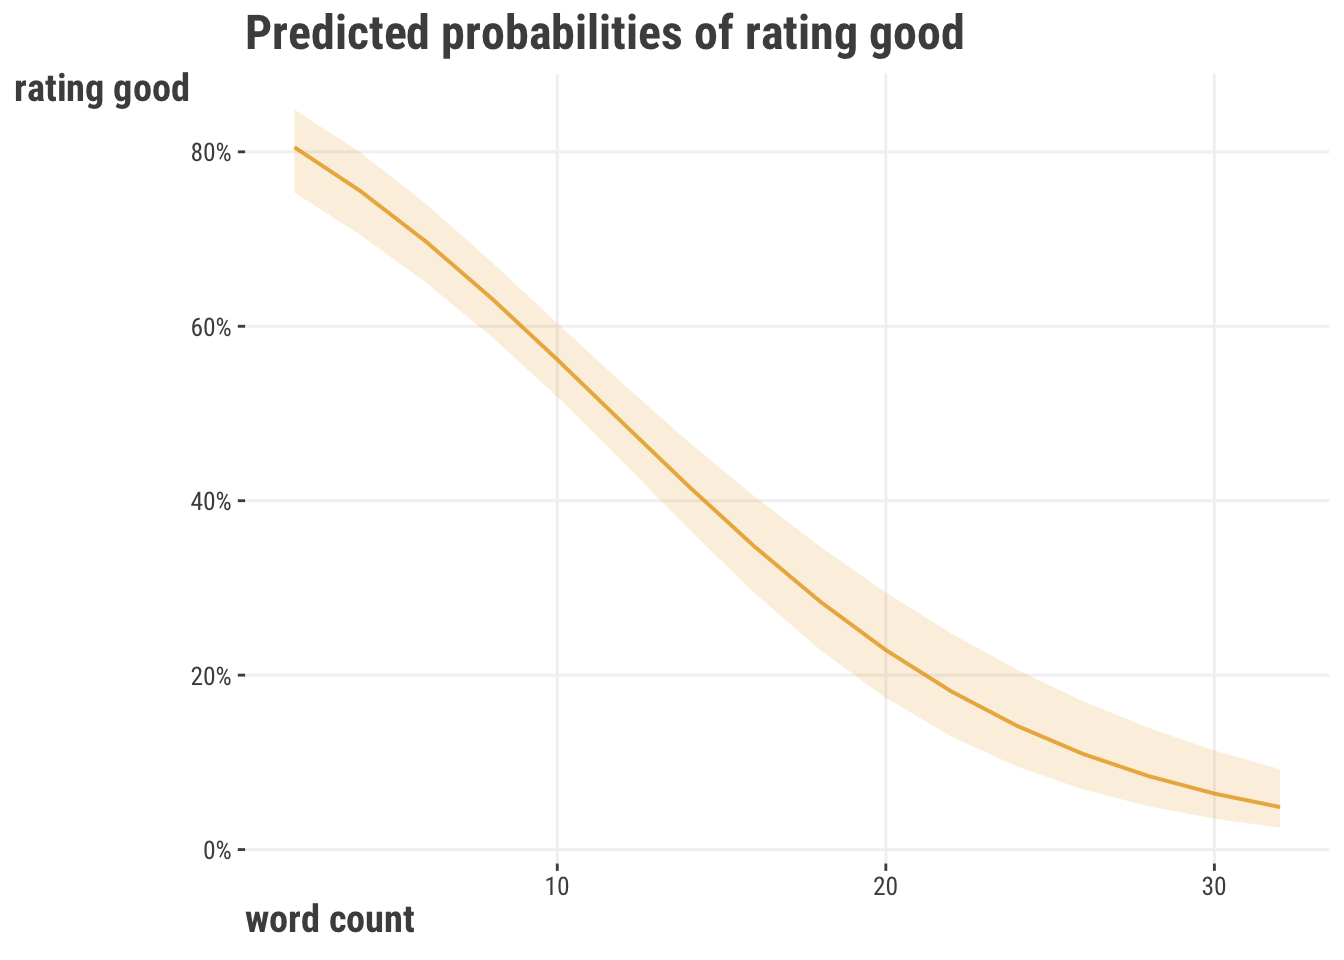
\includegraphics{generalized_linear_models_files/figure-pdf/fig-logistic-regression-count-1.pdf}

}

\caption{\label{fig-logistic-regression-count}Logistic regression
predictions for word count feature}

\end{figure}

In Figure~\ref{fig-logistic-regression-count}, we can see a clear
negative relationship between the number of words in a review and the
probability of being considered a ``good'' movie. As we get over 20
words, the predicted probability of being a ``good'' movie is less than
.2.

\begin{figure}

{\centering 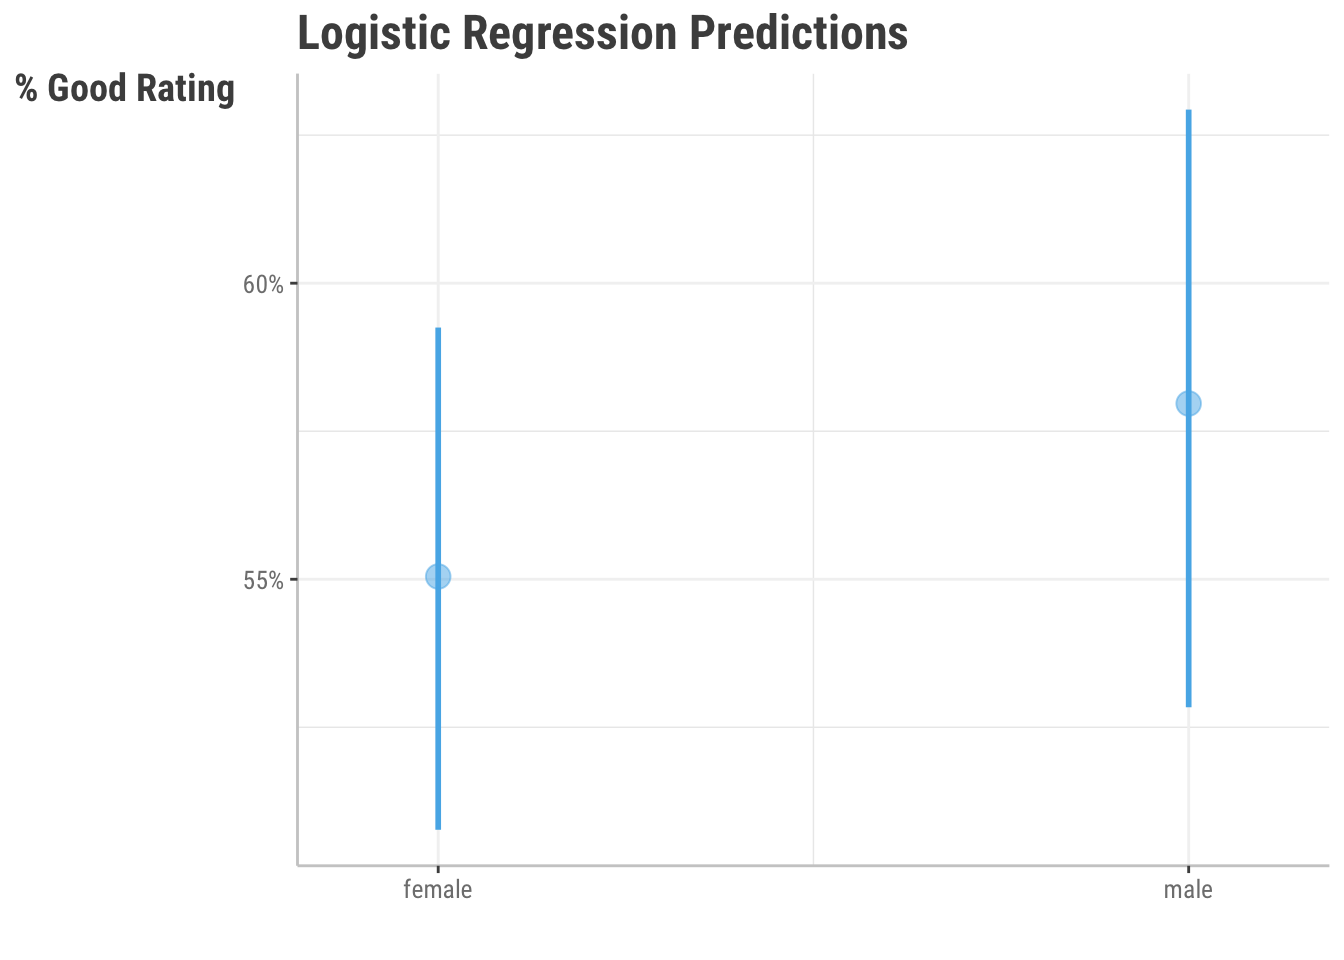
\includegraphics{generalized_linear_models_files/figure-pdf/fig-logistic-regression-gender-1.pdf}

}

\caption{\label{fig-logistic-regression-gender}Logistic regression
predictions for gender feature}

\end{figure}

We can also see the gender effect in
Figure~\ref{fig-logistic-regression-gender} (it doesn't look like gender
is that interesting in this model).

There are interesting issues at play here with regard to our predictor
coefficients (what can be considered a \emph{relative effect}) and the
model's effect as a whole on the probability (the \emph{absolute
effect}). In circumstances where the intercept is very large
(essentially promising a success), the relative effect of a coefficient
is practically meaningless. Similarly, very negative coefficients render
the relative effects useless.

\subsection{Loss Function}\label{loss-function}

Let's see how we can pick that work apart to create our own functions.
We can use maximum likelihood estimation to estimate the parameters of
our model.

\subsubsection{R}

\begin{Shaded}
\begin{Highlighting}[]
\NormalTok{logreg\_ml }\OtherTok{\textless{}{-}} \ControlFlowTok{function}\NormalTok{(par, X, y) \{}
\NormalTok{  beta }\OtherTok{=}\NormalTok{ par}
\NormalTok{  N }\OtherTok{=} \FunctionTok{nrow}\NormalTok{(X)}
\NormalTok{  LP }\OtherTok{=}\NormalTok{ X }\SpecialCharTok{\%*\%}\NormalTok{ beta                           }
\NormalTok{  mu }\OtherTok{=} \FunctionTok{plogis}\NormalTok{(LP)                           }
\NormalTok{  L }\OtherTok{=} \FunctionTok{dbinom}\NormalTok{(y, }\AttributeTok{size =} \DecValTok{1}\NormalTok{, }\AttributeTok{prob =}\NormalTok{ mu, }\AttributeTok{log =} \ConstantTok{TRUE}\NormalTok{)   }
  \SpecialCharTok{{-}}\FunctionTok{sum}\NormalTok{(L)                                   }
\NormalTok{\}}
\end{Highlighting}
\end{Shaded}

\subsubsection{Python}

\begin{Shaded}
\begin{Highlighting}[]
\KeywordTok{def}\NormalTok{ logreg\_ml(par, X, y):}
\NormalTok{    beta }\OperatorTok{=}\NormalTok{ par}
\NormalTok{    N }\OperatorTok{=}\NormalTok{ X.shape[}\DecValTok{0}\NormalTok{]}
\NormalTok{    LP }\OperatorTok{=}\NormalTok{ X.dot(beta).to\_numpy()  }
\NormalTok{    mu }\OperatorTok{=}\NormalTok{ [}\DecValTok{1} \OperatorTok{/}\NormalTok{ (}\DecValTok{1} \OperatorTok{+}\NormalTok{ np.exp(}\OperatorTok{{-}}\NormalTok{x)) }\ControlFlowTok{for}\NormalTok{ x }\KeywordTok{in}\NormalTok{ LP]}
\NormalTok{    mu\_minus\_1 }\OperatorTok{=}\NormalTok{ [}\DecValTok{1} \OperatorTok{{-}}\NormalTok{ x }\ControlFlowTok{for}\NormalTok{ x }\KeywordTok{in}\NormalTok{ mu]}
\NormalTok{    L }\OperatorTok{=}\NormalTok{ y}\OperatorTok{*}\NormalTok{np.log(mu) }\OperatorTok{+}\NormalTok{ (}\DecValTok{1} \OperatorTok{{-}}\NormalTok{ y)}\OperatorTok{*}\NormalTok{np.log(mu\_minus\_1)   }
    \ControlFlowTok{return} \OperatorTok{{-}}\NormalTok{np.}\BuiltInTok{sum}\NormalTok{(L)   }
  
\end{Highlighting}
\end{Shaded}

\subsection{Model Fitting}\label{model-fitting}

Now that we have our loss function, we can fit our model. We will use
the \texttt{optim} function in R and the \texttt{minimize} function in
Python.

\subsubsection{R}

\begin{Shaded}
\begin{Highlighting}[]
\NormalTok{init }\OtherTok{=} \FunctionTok{rep}\NormalTok{(}\DecValTok{0}\NormalTok{, }\FunctionTok{ncol}\NormalTok{(X))}

\FunctionTok{names}\NormalTok{(init) }\OtherTok{=} \FunctionTok{c}\NormalTok{(}\StringTok{\textquotesingle{}intercept\textquotesingle{}}\NormalTok{, }\StringTok{\textquotesingle{}b1\textquotesingle{}}\NormalTok{, }\StringTok{\textquotesingle{}b2\textquotesingle{}}\NormalTok{)}

\NormalTok{fit\_ml }\OtherTok{=} \FunctionTok{optim}\NormalTok{(}
  \AttributeTok{par =}\NormalTok{ init,}
  \AttributeTok{fn  =}\NormalTok{ logreg\_ml,}
  \AttributeTok{X   =}\NormalTok{ X,}
  \AttributeTok{y   =}\NormalTok{ y,}
  \AttributeTok{control =} \FunctionTok{list}\NormalTok{(}\AttributeTok{reltol =} \FloatTok{1e{-}8}\NormalTok{)}
\NormalTok{)}

\NormalTok{pars\_ml }\OtherTok{=}\NormalTok{ fit\_ml}\SpecialCharTok{$}\NormalTok{par}

\NormalTok{pars\_ml}
\end{Highlighting}
\end{Shaded}

\begin{verbatim}
 intercept         b1         b2 
 1.7121816 -0.1463750  0.1189308 
\end{verbatim}

\subsubsection{Python}

\begin{Shaded}
\begin{Highlighting}[]
\ImportTok{import}\NormalTok{ numpy }\ImportTok{as}\NormalTok{ np}
\ImportTok{from}\NormalTok{ scipy.optimize }\ImportTok{import}\NormalTok{ minimize}

\NormalTok{init }\OperatorTok{=}\NormalTok{ np.zeros(X.shape[}\DecValTok{1}\NormalTok{])}

\NormalTok{fit\_ml }\OperatorTok{=}\NormalTok{ minimize(}
\NormalTok{    fun }\OperatorTok{=}\NormalTok{ logreg\_ml,}
\NormalTok{    x0 }\OperatorTok{=}\NormalTok{ init,}
\NormalTok{    args }\OperatorTok{=}\NormalTok{ (X, y),}
\NormalTok{    method }\OperatorTok{=} \StringTok{\textquotesingle{}BFGS\textquotesingle{}}\NormalTok{,}
\NormalTok{    options }\OperatorTok{=}\NormalTok{ \{}\StringTok{\textquotesingle{}disp\textquotesingle{}}\NormalTok{: }\VariableTok{True}\NormalTok{\}}
\NormalTok{)}
\end{Highlighting}
\end{Shaded}

\begin{verbatim}
Optimization terminated successfully.
         Current function value: 628.696593
         Iterations: 11
         Function evaluations: 68
         Gradient evaluations: 17
\end{verbatim}

\begin{Shaded}
\begin{Highlighting}[]
\NormalTok{fit\_ml.x}
\end{Highlighting}
\end{Shaded}

\begin{verbatim}
array([ 1.71240414, -0.14638763,  0.11891015])
\end{verbatim}

\begin{tcolorbox}[enhanced jigsaw, rightrule=.15mm, opacityback=0, left=2mm, bottomrule=.15mm, toprule=.15mm, arc=.35mm, colframe=quarto-callout-important-color-frame, leftrule=.75mm, breakable, colback=white]
\begin{minipage}[t]{5.5mm}
\textcolor{quarto-callout-important-color}{\faExclamation}
\end{minipage}%
\begin{minipage}[t]{\textwidth - 5.5mm}

In theory, there is no such thing as 0 or 1 probability. When your model
encounters such a value, you will receive a warning, not an error. The
most likely cause of this warning is \textbf{separation}: a variable is
perfectly separating the target. In other words, once a feature gets
below/above a certain value, the target is always 0/1. While that
variable is no doubt valuable, it can't be used in a logistic regression
model. More evidence of separation comes when you see your log odds
coefficients return something comically large.

\end{minipage}%
\end{tcolorbox}

\begin{tcolorbox}[enhanced jigsaw, rightrule=.15mm, opacityback=0, left=2mm, bottomrule=.15mm, toprule=.15mm, arc=.35mm, colframe=quarto-callout-warning-color-frame, leftrule=.75mm, breakable, colback=white]
\begin{minipage}[t]{5.5mm}
\textcolor{quarto-callout-warning-color}{\faExclamationTriangle}
\end{minipage}%
\begin{minipage}[t]{\textwidth - 5.5mm}

Logistic regression does not have an \(R^2\) value in the way that a
linear regression model does. Instead, there are pseudo-\(R^2\) values,
but they are not the same as the \(R^2\) value that you are used to
seeing. Here is a great breakdown of different pseudo methods.

\end{minipage}%
\end{tcolorbox}

\section{Poisson Regression}\label{poisson-regression}

\subsection{Why Should You Care}\label{why-should-you-care-1}

Like logistic regression, poisson regression belongs to a broad class of
generalized linear models. Poisson regression is used when you have a
count variable as your target. The nature of a count variable is very
different, since it starts at 0 and can only be a whole number. We need
a model that will not produce negative predictions and poisson
regression will do that for us.

\subsection{The Poisson Distribution}\label{the-poisson-distribution}

The Poisson distribution is very similar to the binomial distribution,
but has some key differences. The biggest difference is in its
parameter: Poisson has a single parameter noted as \(\lambda\). This
rate parameter is going to estimate the expected number of events during
a time interval. This can be accidents in a year, pieces produced in a
day, or hits during the course of a baseball season. We can find the
rate by determining the number of events per interval, multiplied by the
interval length.

\[\frac{\text{event}}{\text{interval}}*\text{interval length} \]

To put some numbers to that, if we have 1 accident per week in a factory
and we are observing a whole year, we would have a rate of
\((1 / 7) * 28 = 4\) accidents per month.

Let's see what that particular distribution might look like in
Figure~\ref{fig-poisson-distribution}:

\begin{figure}

{\centering 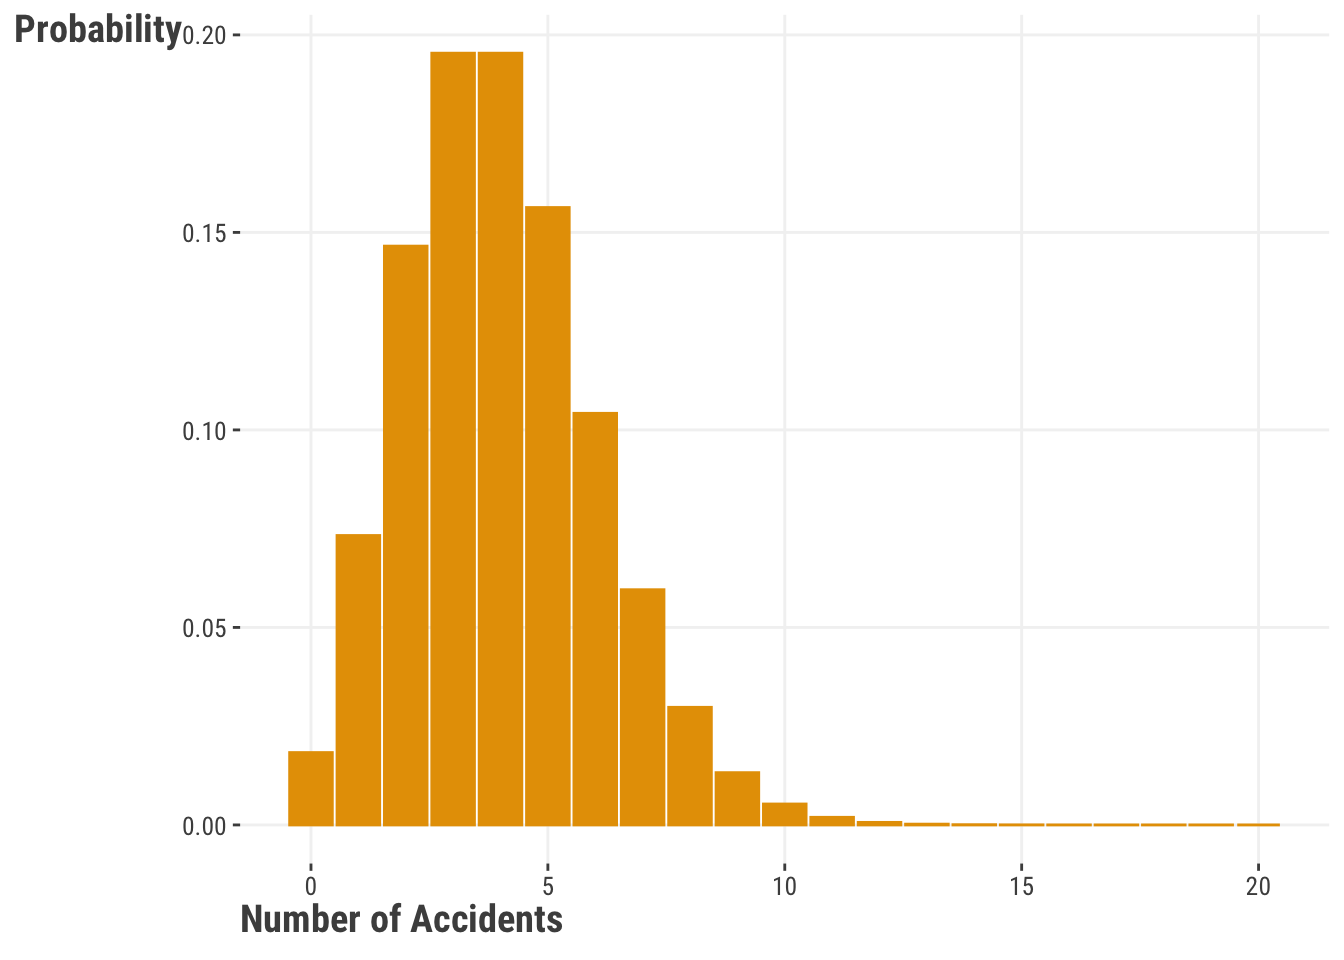
\includegraphics{generalized_linear_models_files/figure-pdf/fig-poisson-distribution-1.pdf}

}

\caption{\label{fig-poisson-distribution}Poisson distribution for a rate
of 4}

\end{figure}

We can also see what it looks like for different rates (some places
might be safer than others) in
Figure~\ref{fig-poisson-distribution-rates}:

\begin{figure}

{\centering 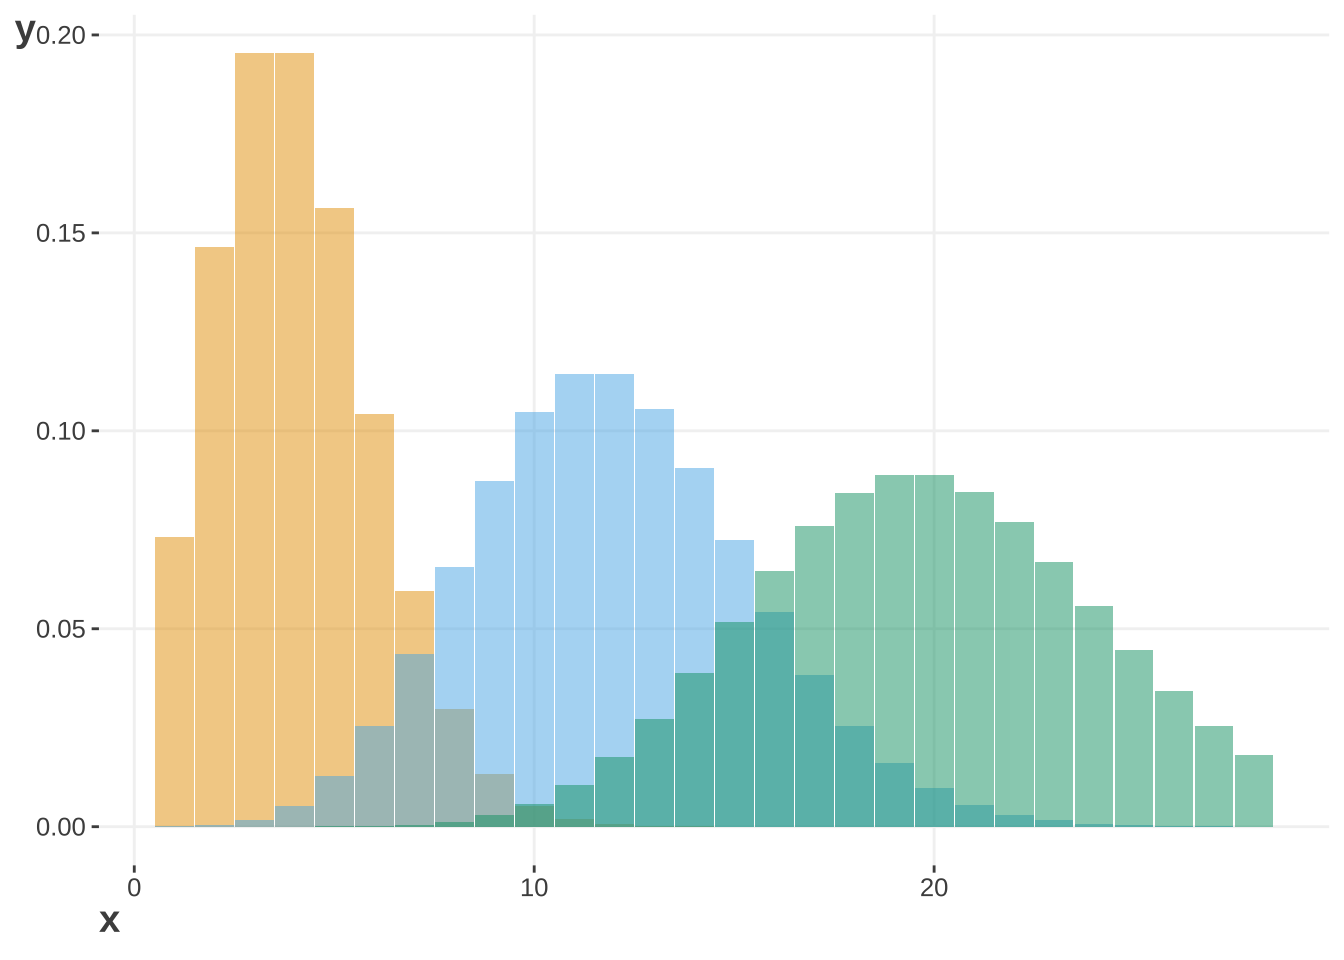
\includegraphics{generalized_linear_models_files/figure-pdf/fig-poisson-distribution-rates-1.pdf}

}

\caption{\label{fig-poisson-distribution-rates}Poisson distributions for
different rates}

\end{figure}

\begin{tcolorbox}[enhanced jigsaw, rightrule=.15mm, opacityback=0, left=2mm, bottomrule=.15mm, toprule=.15mm, arc=.35mm, colframe=quarto-callout-note-color-frame, leftrule=.75mm, breakable, colback=white]
\begin{minipage}[t]{5.5mm}
\textcolor{quarto-callout-note-color}{\faInfo}
\end{minipage}%
\begin{minipage}[t]{\textwidth - 5.5mm}

A cool thing about these distributions is that they can deal with
different \emph{exposure} rates. You don't need observations recorded
over the same interval length, because you can adjust for them
appropriately. They can also be used to model inter-arrival times and
time-until events.

\end{minipage}%
\end{tcolorbox}

Let's make a new variable that will count the number of times a person
uses a personal pronoun word.

\subsubsection{R}

\begin{Shaded}
\begin{Highlighting}[]
\NormalTok{reviews}\SpecialCharTok{$}\NormalTok{poss\_pronoun }\OtherTok{\textless{}{-}}\NormalTok{ stringr}\SpecialCharTok{::}\FunctionTok{str\_count}\NormalTok{(}
\NormalTok{  reviews}\SpecialCharTok{$}\NormalTok{review\_text, }
  \StringTok{"}\SpecialCharTok{\textbackslash{}\textbackslash{}}\StringTok{bI}\SpecialCharTok{\textbackslash{}\textbackslash{}}\StringTok{b|}\SpecialCharTok{\textbackslash{}\textbackslash{}}\StringTok{bme}\SpecialCharTok{\textbackslash{}\textbackslash{}}\StringTok{b|}\SpecialCharTok{\textbackslash{}\textbackslash{}}\StringTok{b[Mm]y}\SpecialCharTok{\textbackslash{}\textbackslash{}}\StringTok{b|}\SpecialCharTok{\textbackslash{}\textbackslash{}}\StringTok{bmine}\SpecialCharTok{\textbackslash{}\textbackslash{}}\StringTok{b|}\SpecialCharTok{\textbackslash{}\textbackslash{}}\StringTok{bmyself}\SpecialCharTok{\textbackslash{}\textbackslash{}}\StringTok{b"}
\NormalTok{)}
\end{Highlighting}
\end{Shaded}

\subsubsection{Python}

\begin{Shaded}
\begin{Highlighting}[]
\NormalTok{reviews[}\StringTok{\textquotesingle{}poss\_pronoun\textquotesingle{}}\NormalTok{] }\OperatorTok{=}\NormalTok{ reviews[}\StringTok{\textquotesingle{}review\_text\textquotesingle{}}\NormalTok{].}\BuiltInTok{str}\NormalTok{.count(}
  \StringTok{\textquotesingle{}"}\CharTok{\textbackslash{}\textbackslash{}}\StringTok{bI}\CharTok{\textbackslash{}\textbackslash{}}\StringTok{b|}\CharTok{\textbackslash{}\textbackslash{}}\StringTok{bme}\CharTok{\textbackslash{}\textbackslash{}}\StringTok{b|}\CharTok{\textbackslash{}\textbackslash{}}\StringTok{b[Mm]y}\CharTok{\textbackslash{}\textbackslash{}}\StringTok{b|}\CharTok{\textbackslash{}\textbackslash{}}\StringTok{bmine}\CharTok{\textbackslash{}\textbackslash{}}\StringTok{b|}\CharTok{\textbackslash{}\textbackslash{}}\StringTok{bmyself}\CharTok{\textbackslash{}\textbackslash{}}\StringTok{b"\textquotesingle{}}
\NormalTok{  )}
\end{Highlighting}
\end{Shaded}

\section{The (Sometimes) Thin Line}\label{the-sometimes-thin-line}

This gets into an area where we need to think long and hard about our
dependent variable and what it actually might be. Since Poisson
regression gets its name from the Poisson distribution, we should
probably see if it follows the Poisson distribution.

\begin{verbatim}

     Goodness-of-fit test for poisson distribution

                      X^2 df  P(> X^2)
Likelihood Ratio 2.283728  3 0.5156453
\end{verbatim}

This is a \(\chi^2\) to test if the distribution deviates from a
Poisson. If we see a significant value, we would say that it deviates
from the tested distribution. In this case, it is pretty clear that
\texttt{poss\_pronoun} could come from a Poisson distribution.

We can also plot that test using a hanging rootogram:

\begin{figure}

{\centering 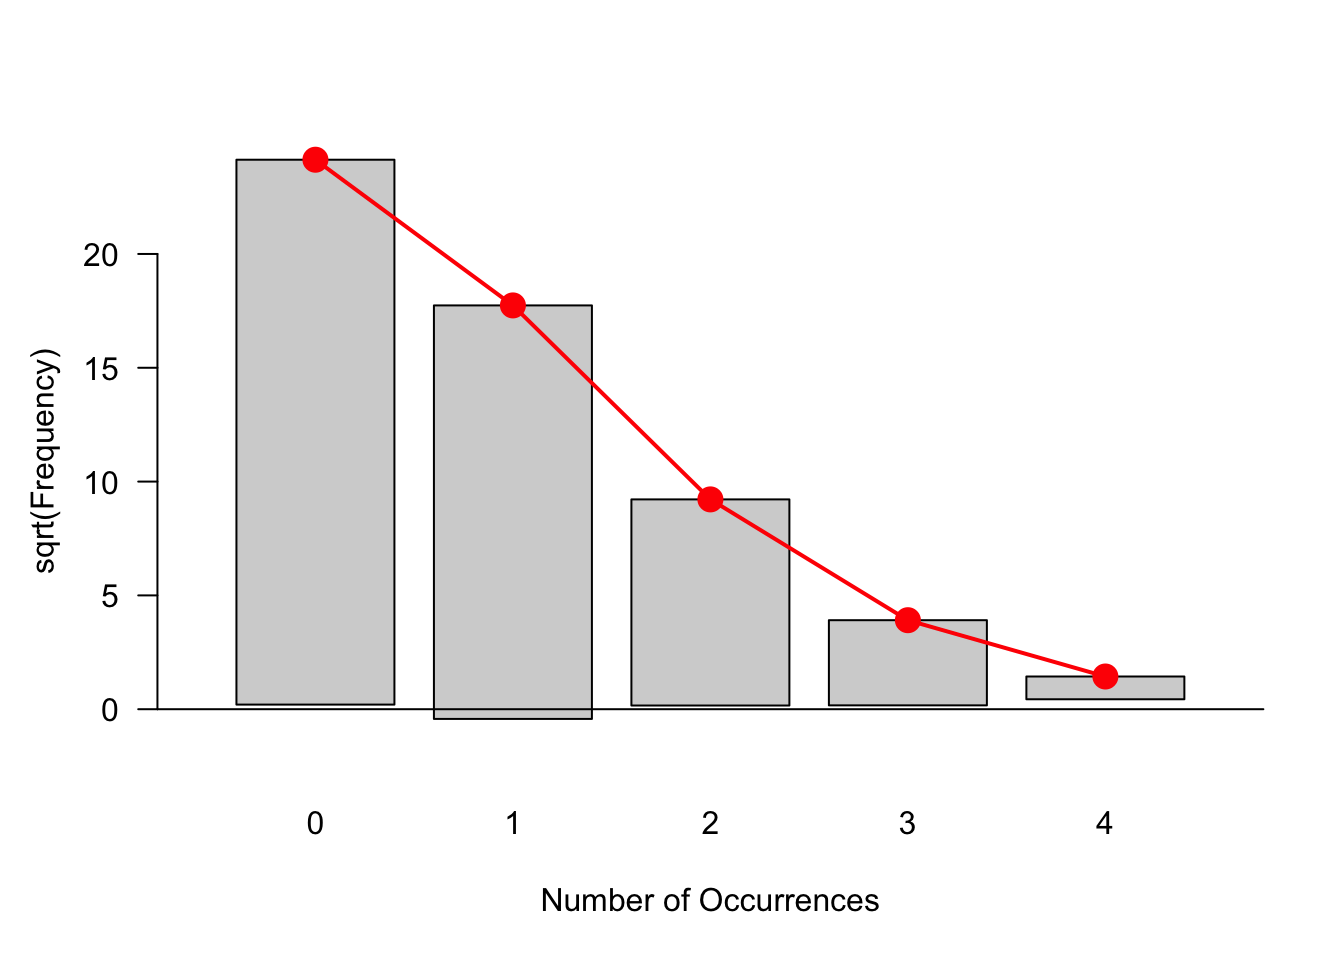
\includegraphics{generalized_linear_models_files/figure-pdf/fig-poisson-test-1.pdf}

}

\caption{\label{fig-poisson-test}Hanging rootogram for Poisson
distribution}

\end{figure}

In Figure~\ref{fig-poisson-test}, the bars are the observed counts and
the red line/points are the fitted counts (i.e., how many would be
expected). If a bar does not reach the 0 line, then the model would
over-predict for that particular count; if the bar dips below the 0
line, the model under-predicts that count. It looks like we are pretty
close for our counts.

\subsection{Standard Functions}\label{standard-functions-1}

Recall that every distribution has a link function (or several) that
tend to work well for it. The poisson distribution uses a log link
function:

\[y = Poisson(\lambda) \\ \text{log}(\lambda) = \alpha + \beta X\]

Using the log link keeps the outcome positive (we cannot deal with
negative counts). Logs, as they are prone to do, are going to tend
towards an exponential relationship; just be sure that it makes sense
over the entire range of your data.

\subsubsection{R}

\begin{Shaded}
\begin{Highlighting}[]
\NormalTok{poisson\_test }\OtherTok{\textless{}{-}} \FunctionTok{glm}\NormalTok{(poss\_pronoun }\SpecialCharTok{\textasciitilde{}}\NormalTok{ word\_count,}
                  \AttributeTok{data =}\NormalTok{ reviews,}
                  \AttributeTok{family =}\NormalTok{ poisson)}

\FunctionTok{summary}\NormalTok{(poisson\_test)}
\end{Highlighting}
\end{Shaded}

\begin{verbatim}

Call:
glm(formula = poss_pronoun ~ word_count, family = poisson, data = reviews)

Coefficients:
             Estimate Std. Error z value Pr(>|z|)    
(Intercept) -1.848982   0.099409  -18.60   <2e-16 ***
word_count   0.103126   0.006433   16.03   <2e-16 ***
---
Signif. codes:  0 '***' 0.001 '**' 0.01 '*' 0.05 '.' 0.1 ' ' 1

(Dispersion parameter for poisson family taken to be 1)

    Null deviance: 996.21  on 999  degrees of freedom
Residual deviance: 776.19  on 998  degrees of freedom
AIC: 1699.7

Number of Fisher Scoring iterations: 5
\end{verbatim}

\begin{Shaded}
\begin{Highlighting}[]
\FunctionTok{exp}\NormalTok{(poisson\_test}\SpecialCharTok{$}\NormalTok{coefficients)}
\end{Highlighting}
\end{Shaded}

\begin{verbatim}
(Intercept)  word_count 
  0.1573974   1.1086314 
\end{verbatim}

\subsubsection{Python}

\begin{Shaded}
\begin{Highlighting}[]
\ImportTok{import}\NormalTok{ statsmodels.api }\ImportTok{as}\NormalTok{ sm}
\ImportTok{import}\NormalTok{ statsmodels.formula.api }\ImportTok{as}\NormalTok{ smf}

\NormalTok{poisson\_test }\OperatorTok{=}\NormalTok{ smf.glm(formula }\OperatorTok{=} \StringTok{"poss\_pronoun \textasciitilde{} word\_count"}\NormalTok{,}
\NormalTok{                       data }\OperatorTok{=}\NormalTok{ reviews,}
\NormalTok{                       family }\OperatorTok{=}\NormalTok{ sm.families.Poisson()).fit()}

\NormalTok{poisson\_test.summary()        }
\end{Highlighting}
\end{Shaded}

\begin{verbatim}
<class 'statsmodels.iolib.summary.Summary'>
"""
                 Generalized Linear Model Regression Results                  
==============================================================================
Dep. Variable:           poss_pronoun   No. Observations:                 1000
Model:                            GLM   Df Residuals:                      998
Model Family:                 Poisson   Df Model:                            1
Link Function:                    Log   Scale:                          1.0000
Method:                          IRLS   Log-Likelihood:                -583.89
Date:                Sat, 09 Dec 2023   Deviance:                       689.32
Time:                        10:21:14   Pearson chi2:                     785.
No. Iterations:                     5   Pseudo R-squ. (CS):           0.008438
Covariance Type:            nonrobust                                         
==============================================================================
                 coef    std err          z      P>|z|      [0.025      0.975]
------------------------------------------------------------------------------
Intercept     -1.7900      0.144    -12.415      0.000      -2.073      -1.507
word_count     0.0344      0.011      3.011      0.003       0.012       0.057
==============================================================================
"""
\end{verbatim}

\begin{Shaded}
\begin{Highlighting}[]
\NormalTok{np.exp(poisson\_test.params)}
\end{Highlighting}
\end{Shaded}

\begin{verbatim}
Intercept     0.166965
word_count    1.035001
dtype: float64
\end{verbatim}

We are going to interpret this almost the same as a linear regression.
The slight wrinkle here, though, is that we are looking at the log
counts (remember that we specified the log link function). In other
words, an increase in one one review word leads to an expected log count
increase of \textasciitilde.01. Just like our logisitc regression, we
could exponentiate this to get 1.108 -- every added word in a review
gets us a \textasciitilde1\% increase in the number of possessive
pronouns. Let's see what this looks like in action in
Figure~\ref{fig-poisson-regression}:

\begin{figure}

{\centering 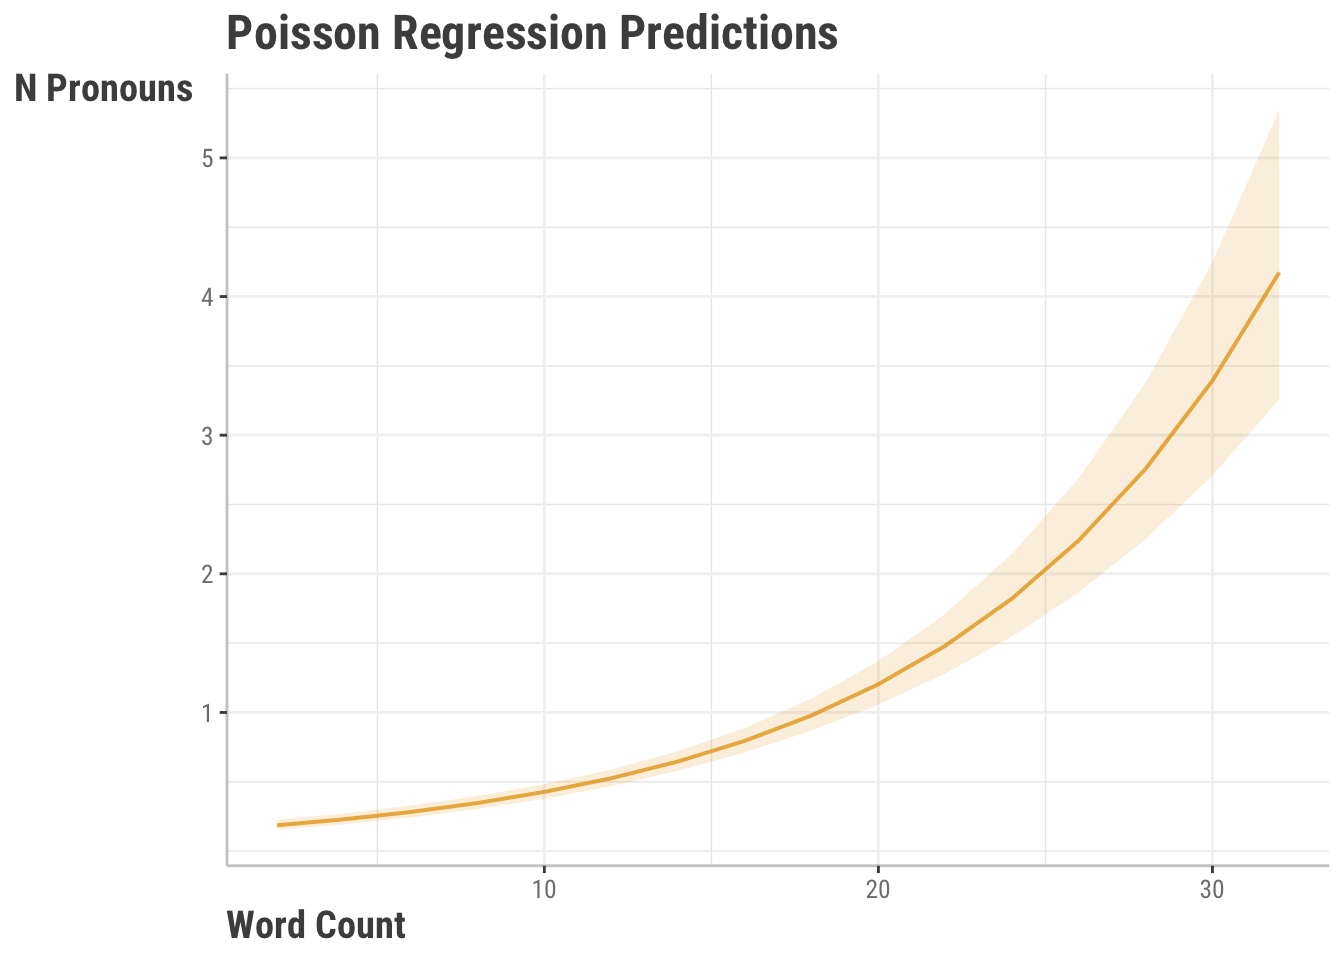
\includegraphics{generalized_linear_models_files/figure-pdf/fig-poisson-regression-1.pdf}

}

\caption{\label{fig-poisson-regression}Poisson regression predictions
for word count feature}

\end{figure}

With everything coupled together, we have a meaningful coefficient for
\texttt{word\_count}, a clear plot, and adequate model fit. Therefore,
we might conclude that there is a positive relationship between number
of words in a review on the number of times a person uses a personal
possessive.

\begin{verbatim}

    Overdispersion test

data:  poisson_test
z = -8.0493, p-value = 1
alternative hypothesis: true dispersion is greater than 1
sample estimates:
dispersion 
 0.7606014 
\end{verbatim}

The dispersion value that we see returned (0.7606014 in our case) should
be under 1. A dispersion value over 1 means that we have overdispersion.
Our dispersion value, coupled with our high \emph{p}-value, indicates
that we would fail to reject the null hypothesis of equidispersion.

We can also look back to our model results to compare our residual
deviance to our residual deviance degrees of freedom; if our deviance is
greater than our degrees of freedom, we might have an issue with
overdispersion. Since we are just a bit over and our overdispersion
tests do not indicate any huge issue, we can be relatively okay with our
model. If we had some more extreme overdispersion, we would want to flip
to a quasi-poisson distribution -- our coefficients would not change,
but we would have improved standard errors.

\subsection{Model Specification}\label{model-specification}

\subsubsection{R}

\begin{Shaded}
\begin{Highlighting}[]
\NormalTok{pois\_ll }\OtherTok{\textless{}{-}} \ControlFlowTok{function}\NormalTok{(y, X, par) \{}
\NormalTok{  beta }\OtherTok{\textless{}{-}}\NormalTok{ par}
\NormalTok{  lambda }\OtherTok{\textless{}{-}} \FunctionTok{exp}\NormalTok{(beta}\SpecialCharTok{\%*\%}\FunctionTok{t}\NormalTok{(X))}
\NormalTok{  loglik }\OtherTok{\textless{}{-}} \SpecialCharTok{{-}}\FunctionTok{sum}\NormalTok{(}\FunctionTok{dpois}\NormalTok{(y, lambda, }\AttributeTok{log =} \ConstantTok{TRUE}\NormalTok{))}
  \FunctionTok{return}\NormalTok{(loglik)}
\NormalTok{\}}
\end{Highlighting}
\end{Shaded}

\subsubsection{Python}

\begin{Shaded}
\begin{Highlighting}[]
\ImportTok{from}\NormalTok{ scipy.stats }\ImportTok{import}\NormalTok{ poisson}

\KeywordTok{def}\NormalTok{ pois\_ll(par, X, y):}
\NormalTok{    beta }\OperatorTok{=}\NormalTok{ par}
\NormalTok{    lambda\_ }\OperatorTok{=}\NormalTok{ np.exp(X.dot(beta))}
\NormalTok{    loglik }\OperatorTok{=} \OperatorTok{{-}}\NormalTok{np.}\BuiltInTok{sum}\NormalTok{(poisson.logpmf(y, lambda\_))}
    \ControlFlowTok{return}\NormalTok{ loglik}
\end{Highlighting}
\end{Shaded}

\subsection{Model Fitting}\label{model-fitting-1}

\subsubsection{R}

\begin{Shaded}
\begin{Highlighting}[]
\NormalTok{form }\OtherTok{\textless{}{-}} \FunctionTok{as.formula}\NormalTok{(}\StringTok{"poss\_pronoun \textasciitilde{} word\_count"}\NormalTok{)}
\NormalTok{model }\OtherTok{\textless{}{-}} \FunctionTok{model.frame}\NormalTok{(form, }\AttributeTok{data =}\NormalTok{ reviews)}
\NormalTok{X }\OtherTok{\textless{}{-}} \FunctionTok{model.matrix}\NormalTok{(form, }\AttributeTok{data =}\NormalTok{ reviews)}
\NormalTok{y }\OtherTok{\textless{}{-}} \FunctionTok{model.response}\NormalTok{(model)}

\NormalTok{starts }\OtherTok{\textless{}{-}} \FunctionTok{c}\NormalTok{(}\DecValTok{0}\NormalTok{, }\DecValTok{0}\NormalTok{)}

\NormalTok{fit }\OtherTok{=} \FunctionTok{optim}\NormalTok{(}
  \AttributeTok{par =}\NormalTok{ starts ,}
  \AttributeTok{fn  =}\NormalTok{ pois\_ll,}
  \AttributeTok{X   =}\NormalTok{ X,}
  \AttributeTok{y   =}\NormalTok{ y,}
  \AttributeTok{method  =} \StringTok{"BFGS"}\NormalTok{,}
  \AttributeTok{control =} \FunctionTok{list}\NormalTok{(}\AttributeTok{maxit =} \DecValTok{5000}\NormalTok{, }\AttributeTok{reltol =} \FloatTok{1e{-}12}\NormalTok{),}
  \AttributeTok{hessian =} \ConstantTok{TRUE}
\NormalTok{)}

\NormalTok{fit}\SpecialCharTok{$}\NormalTok{par}
\end{Highlighting}
\end{Shaded}

\begin{verbatim}
[1] -1.8487431  0.1031103
\end{verbatim}

\subsubsection{Python}

\begin{Shaded}
\begin{Highlighting}[]
\NormalTok{X }\OperatorTok{=}\NormalTok{ reviews[[}\StringTok{\textquotesingle{}word\_count\textquotesingle{}}\NormalTok{]]}

\NormalTok{y }\OperatorTok{=}\NormalTok{ reviews[}\StringTok{"poss\_pronoun"}\NormalTok{]}

\NormalTok{init }\OperatorTok{=}\NormalTok{ np.zeros(X.shape[}\DecValTok{1}\NormalTok{])}

\NormalTok{fit }\OperatorTok{=}\NormalTok{ minimize(}
\NormalTok{    fun }\OperatorTok{=}\NormalTok{ pois\_ll,}
\NormalTok{    x0 }\OperatorTok{=}\NormalTok{ init,}
\NormalTok{    args }\OperatorTok{=}\NormalTok{ (X, y),}
\NormalTok{    method }\OperatorTok{=} \StringTok{\textquotesingle{}BFGS\textquotesingle{}}\NormalTok{,}
\NormalTok{    options }\OperatorTok{=}\NormalTok{ \{}\StringTok{\textquotesingle{}disp\textquotesingle{}}\NormalTok{: }\VariableTok{True}\NormalTok{\}}
\NormalTok{)}
\end{Highlighting}
\end{Shaded}

\begin{verbatim}
Optimization terminated successfully.
         Current function value: 667.282560
         Iterations: 9
         Function evaluations: 22
         Gradient evaluations: 11
\end{verbatim}

\begin{Shaded}
\begin{Highlighting}[]
\NormalTok{fit.x}
\end{Highlighting}
\end{Shaded}

\begin{verbatim}
array([-0.11938671])
\end{verbatim}

\section{Wrapping Up}\label{wrapping-up-1}

These are just two of the many models that fall under the broad umbrella
of generalized linear models. Depending on your data situation, you
might want to keep Figure~\ref{fig-glm-models} in mind:

\begin{figure}

{\centering 

\hypertarget{fig-glm-models-1}{}
\begin{longtable*}{ll}
\toprule
Target & Distribution \\ 
\midrule\addlinespace[2.5pt]
Proportions & beta \\ 
Exponential response & gamma \\ 
3+ categories & multinomial \\ 
Count & negative binomial \\ 
\bottomrule
\end{longtable*}

}

\caption{\label{fig-glm-models}Targets and distributions for generalized
linear models}

\end{figure}

That is, however, just a tiny slice of the potential distributions that
you might find yourself needing to use in a GLM. While you could always
use the general linear model, the key is to understand the distribution
of your target and then find the appropriate link function to connect it
to the linear model. Using the proper distribution will always yield
better results and get your model a little closer to the ``truth''.

\section{Additional Resources}\label{additional-resources-1}

In any given graduate coursework, you might find a whole semester
dedicated to GLMs. We've only scratched the surface here, but there are
some great resources out there to help you dig deeper. If you are
itching for a text book, there isn't any shortage of them out there and
you can essentially take your pick. If you are looking for something a
bit more applied, you might want to check out Roback and Legler's
\emph{Beyond Multiple Linear Regression}, available for free at
\url{https://bookdown.org/roback/bookdown-BeyondMLR/}

\chapter{Beyond the Basics}\label{beyond-the-basics}

\section{Quantile Regression}\label{quantile-regression}

\begin{quote}
Oh, you think the mean is your ally. But you merely adopted the mean; I
was born in it, molded by it. I didn't see anything interesting until I
was already a man. And by then, it was nothing to me but illuminating.
-- Bane (probably)
\end{quote}

People generally understand the concept of the arithmetic mean. You see
it some time during elementary school, it gets tossed around in daily
language (usually using the word ``average''), and it is statistically
important. After all, where would the normal distribution be without a
mean? Why, though, do we feel so tied to it from a regression modeling
perspective? Yes, it has handy features, but it is also a bit
restrictive to the types of relationships that it can actually model
well.

In this chapter, we want to show you what to do when the mean betrays
you -- and trust us, the mean will betray you at some point.

\subsection{Why Should You Care?}\label{why-should-you-care-2}

When fitting a line through the mean doesn't make sense, whether due to
extreme scores or you're interested at how your model is performing in
different parts of your data, quantile regression can be helpful.
Quantile regression will give you the ability to model the relationship
between your features and target at different quantiles of your target.
Maybe people who are older are more likely to rate movies higher, but
that relationship is stronger for people who rate movies higher than the
median. Quantile regression will let you model that relationship.

\subsection{When The Mean Breaks Down}\label{when-the-mean-breaks-down}

In a perfect data world, the mean is equal to the middle observation of
the data: the \emph{median}. That is only in the perfect world, though,
and usually our data comes loaded with challenges. Extreme scores in
your data will cause a rift between the median and the mean.

Let's say we take the integers between 1 and 10, and find the mean.

\[\frac{1+2+3+4+5+6+7+8+9+10}{10} =  5.5\]

The middle value in that vector of numbers would also be 5.5.

What happens we replace the 1 with a more extreme value, like -10?

\[\frac{-10+2+3+4+5+6+7+8+9+10}{10} =  4.5\]

With just one dramatic change, our mean went down by a whole point. The
median observation, though, is still 5.5. In short, the median is
invariant to wild swings out in the tails of your numbers.

You might be saying to yourself, ``Why should I care about this central
tendency chicanery?'' Let us tell you why you should care -- the least
squares approach to the standard linear model dictates that the
regression line needs to be fit through the means of the variables. If
you have extreme scores that influence the mean, then your regression
line will also be influenced by those extreme scores.

Let's look at a few different regression lines:

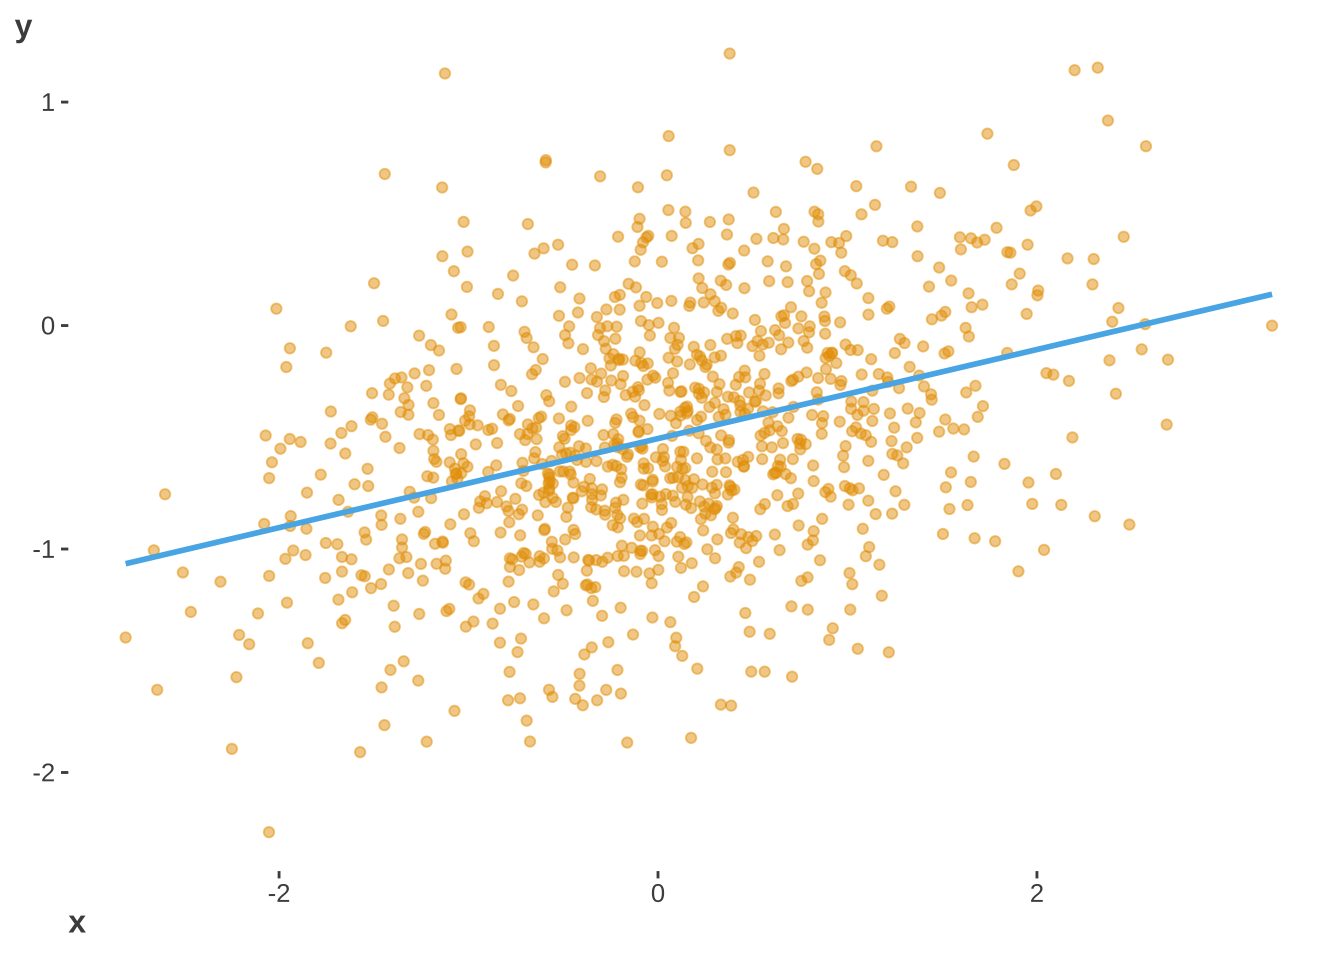
\includegraphics{linear_model_extensions_files/figure-pdf/linear_line_no_extremes-1.pdf}

Now, what would happen if we replaced a few of our observations with
extreme scores?

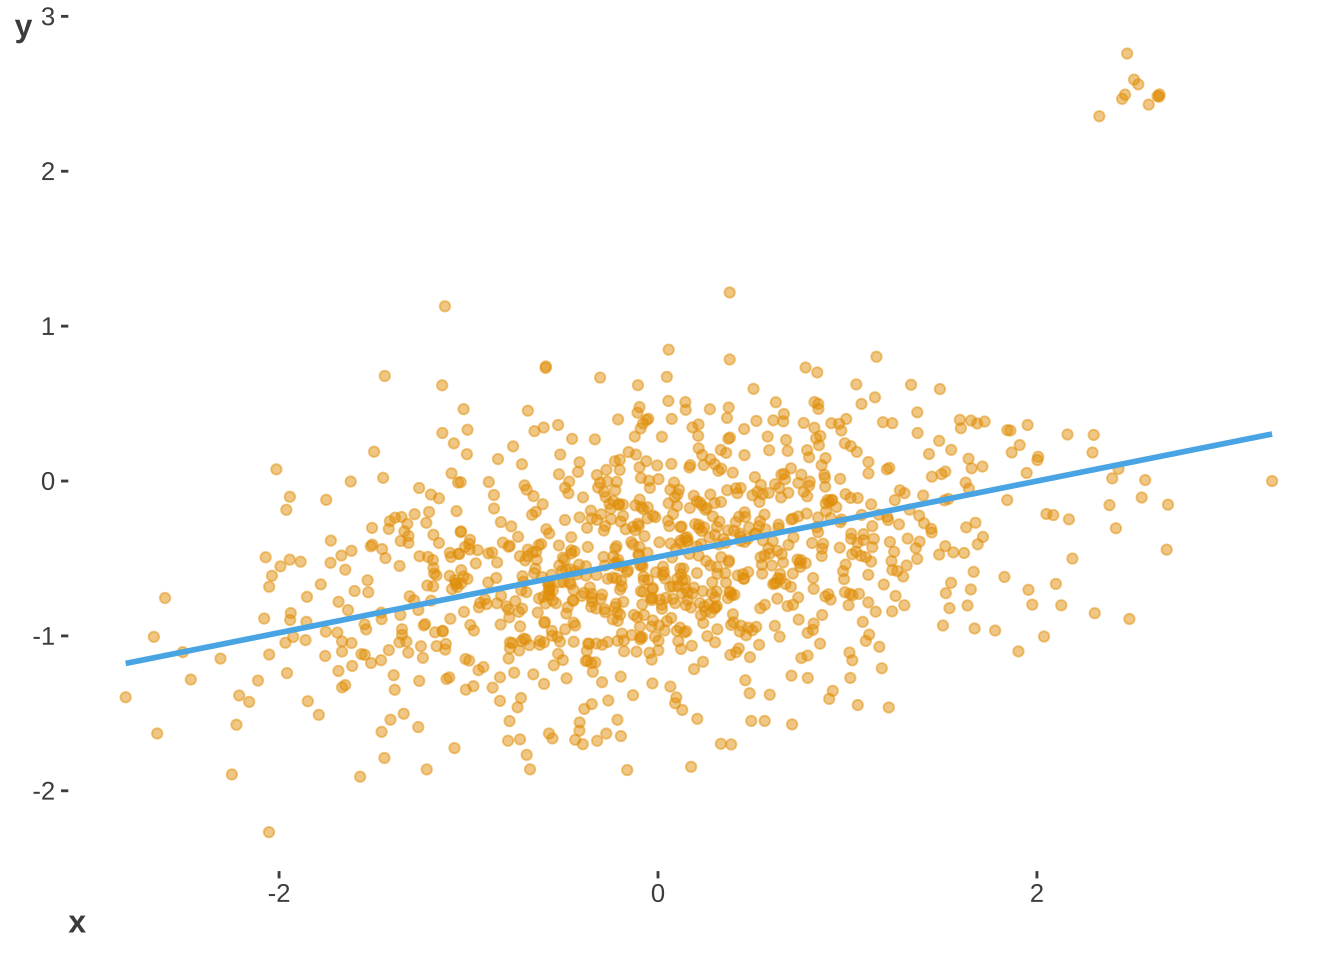
\includegraphics{linear_model_extensions_files/figure-pdf/linear_line_extremes-1.pdf}

With just a casual glance, it doesn't look like our two regression lines
are that different. They both look like they have a similar positive
slope, so all should be good. To offer a bit more clarity, though, let's
put those lines in the same space:

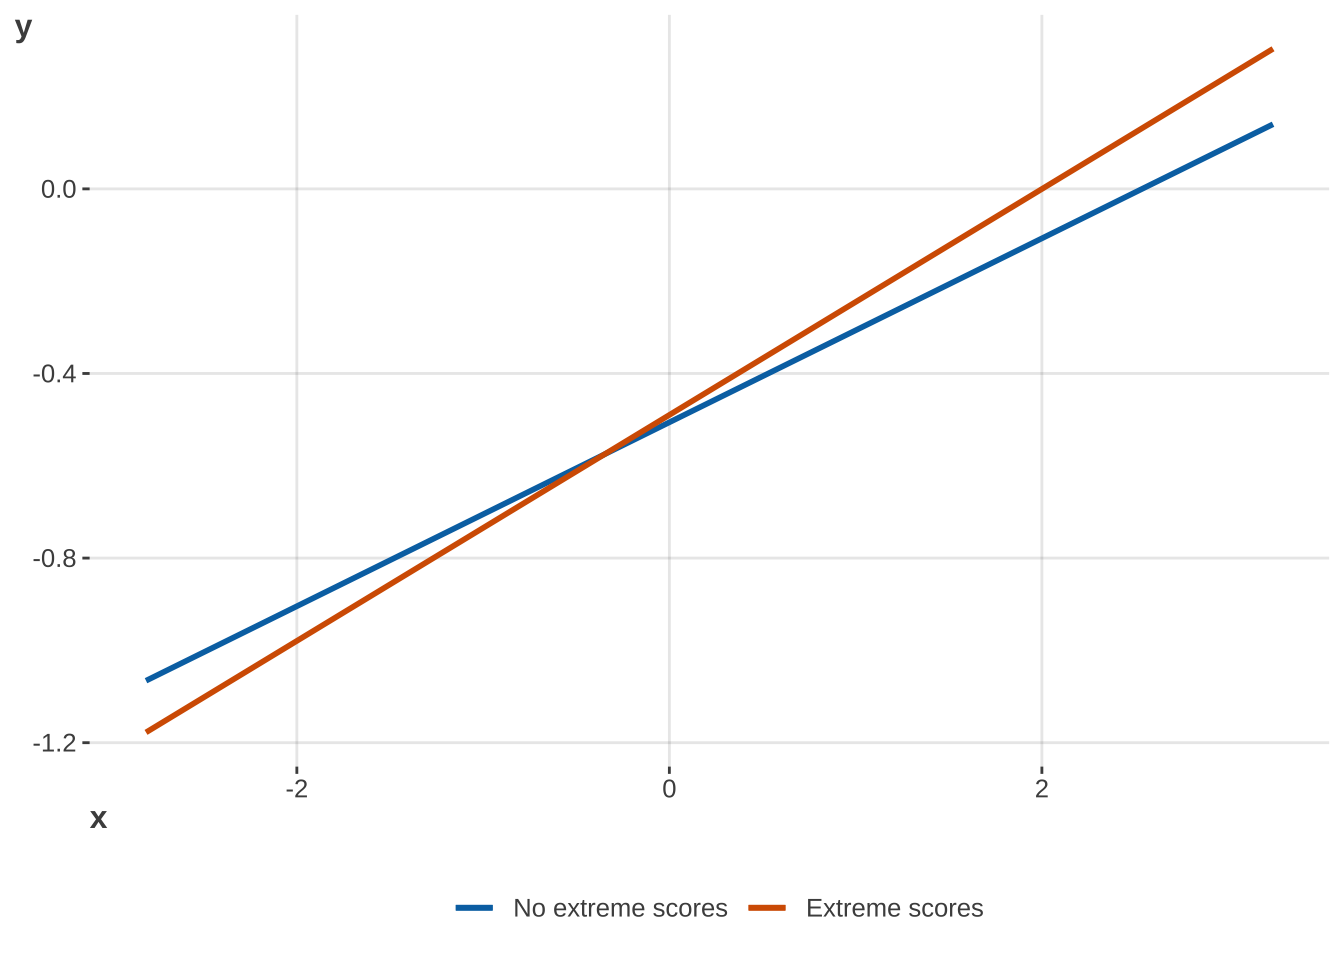
\includegraphics{linear_model_extensions_files/figure-pdf/both_linear_lines-1.pdf}

With 1000 observations, we see that having just 10 extreme scores is
enough to change the regression line, even if just a little. There are a
few approaches we could take here, with common approaches being dropping
those observations or Windsorizing them. Throwing away data because you
don't like the way it behaves is nearing on statistical abuse and
Windsorization is just replacing those extreme values with numbers that
you like a little bit better.

A better answer to this challenge might be to not fit the regression
line through the mean, but the median instead. This is where quantile
regression becomes handy. Formally, this model can be expressed as:

\[
Q_{Y\vert X}(\tau) = X\beta_\tau
\]

Where we can find the estimation of \(\beta_\tau\) as:

\[
\hat\beta_\tau = \arg \min_{\beta \in \mathbb{R}^k} \sum_{i-1}^n(\rho_\tau(Y_i-X_i\beta))
\]

With quantile regression, we are given an extra parameter for the model:
\(\tau\) or \emph{tau}. The tau parameter let's us choose which quantile
we want to use for our line fitting. Since the median splits the data in
half, we can translate that to a quantile of .5.

\subsection{Data Import and
Preparation}\label{data-import-and-preparation-1}

Let's bring in our movie reviews data. Let's say that we are curious
about the relationship between the \texttt{total\_reviews} variable and
the \texttt{rating} variable. First, we need to get our data ready for
our home-brewed functions.

\subsubsection{R}

\begin{Shaded}
\begin{Highlighting}[]
\NormalTok{reviews }\OtherTok{\textless{}{-}} \FunctionTok{read.csv}\NormalTok{(}\StringTok{"data/movie\_reviews\_processed.csv"}\NormalTok{)}

\NormalTok{reviews }\OtherTok{\textless{}{-}} \FunctionTok{na.omit}\NormalTok{(reviews)}

\NormalTok{X }\OtherTok{\textless{}{-}}\NormalTok{ reviews}\SpecialCharTok{$}\NormalTok{total\_reviews}
\NormalTok{X }\OtherTok{\textless{}{-}} \FunctionTok{cbind}\NormalTok{(}\DecValTok{1}\NormalTok{, X)}
\NormalTok{y }\OtherTok{\textless{}{-}}\NormalTok{ reviews}\SpecialCharTok{$}\NormalTok{rating}
\end{Highlighting}
\end{Shaded}

\subsubsection{Python}

\begin{Shaded}
\begin{Highlighting}[]
\ImportTok{import}\NormalTok{ pandas }\ImportTok{as}\NormalTok{ pd}
\ImportTok{import}\NormalTok{ numpy }\ImportTok{as}\NormalTok{ np}

\NormalTok{reviews }\OperatorTok{=}\NormalTok{ pd.read\_csv(}\StringTok{"data/movie\_reviews\_processed.csv"}\NormalTok{)}

\NormalTok{reviews }\OperatorTok{=}\NormalTok{ reviews.dropna()}

\NormalTok{X }\OperatorTok{=}\NormalTok{ pd.DataFrame(}
\NormalTok{  \{}\StringTok{\textquotesingle{}intercept\textquotesingle{}}\NormalTok{: }\DecValTok{1}\NormalTok{, }
  \StringTok{\textquotesingle{}total\_reviews\textquotesingle{}}\NormalTok{: reviews[}\StringTok{\textquotesingle{}total\_reviews\textquotesingle{}}\NormalTok{]\}}
\NormalTok{)}
\NormalTok{y }\OperatorTok{=}\NormalTok{ reviews[}\StringTok{\textquotesingle{}rating\textquotesingle{}}\NormalTok{]}
\end{Highlighting}
\end{Shaded}

\subsection{Standard Functions}\label{standard-functions-2}

We can see how we can use \texttt{quantreg} and \texttt{statsmodels} to
create a quantile regression. For both, we will start with a median
regression; in other words, a quantile of .5.

\subsubsection{R}

\begin{Shaded}
\begin{Highlighting}[]
\FunctionTok{library}\NormalTok{(quantreg)}

\NormalTok{median\_test }\OtherTok{\textless{}{-}} \FunctionTok{rq}\NormalTok{(rating }\SpecialCharTok{\textasciitilde{}}\NormalTok{ total\_reviews, }\AttributeTok{tau =}\NormalTok{ .}\DecValTok{5}\NormalTok{, }
                \AttributeTok{data =}\NormalTok{ reviews)}

\FunctionTok{summary}\NormalTok{(median\_test)}
\end{Highlighting}
\end{Shaded}

\begin{verbatim}

Call: rq(formula = rating ~ total_reviews, tau = 0.5, data = reviews)

tau: [1] 0.5

Coefficients:
              coefficients lower bd upper bd
(Intercept)   2.70278      2.53409  2.77655 
total_reviews 0.00007      0.00006  0.00010 
\end{verbatim}

\subsubsection{Python}

\begin{Shaded}
\begin{Highlighting}[]
\ImportTok{import}\NormalTok{ statsmodels.formula.api }\ImportTok{as}\NormalTok{ smf}

\NormalTok{median\_test }\OperatorTok{=}\NormalTok{ smf.quantreg(}\StringTok{\textquotesingle{}rating \textasciitilde{} total\_reviews\textquotesingle{}}\NormalTok{, }
\NormalTok{                           data }\OperatorTok{=}\NormalTok{ reviews).fit(q }\OperatorTok{=} \FloatTok{.5}\NormalTok{)}
                           
\NormalTok{median\_test.summary()                           }
\end{Highlighting}
\end{Shaded}

\begin{verbatim}
<class 'statsmodels.iolib.summary.Summary'>
"""
                         QuantReg Regression Results                          
==============================================================================
Dep. Variable:                 rating   Pseudo R-squared:              0.05241
Model:                       QuantReg   Bandwidth:                      0.3092
Method:                 Least Squares   Sparsity:                        1.645
Date:                Sat, 09 Dec 2023   No. Observations:                 1000
Time:                        10:38:15   Df Residuals:                      998
                                        Df Model:                            1
=================================================================================
                    coef    std err          t      P>|t|      [0.025      0.975]
---------------------------------------------------------------------------------
Intercept         2.6929      0.052     51.706      0.000       2.591       2.795
total_reviews  7.361e-05   9.17e-06      8.029      0.000    5.56e-05    9.16e-05
=================================================================================

The condition number is large, 1.14e+04. This might indicate that there are
strong multicollinearity or other numerical problems.
"""
\end{verbatim}

Fortunately, our interpretation of this result isn't all that different
from a standard linear model -- the ratings should increase by .00007
for every additional review. However, this is at the median, not the
mean, like the standard linear model.

Quantile regression is not a one-trick-pony. Remember, it is called
quantile regression -- not median regression. Being able to compute a
median regression is just a nice by-product. What we can do with
quantile regression is to model different quantiles of the same data. It
gives us the ability to answer brand new questions -- does the
relationship between user age and their ratings change at different
quantiles of rating?

\begin{figure}

{\centering 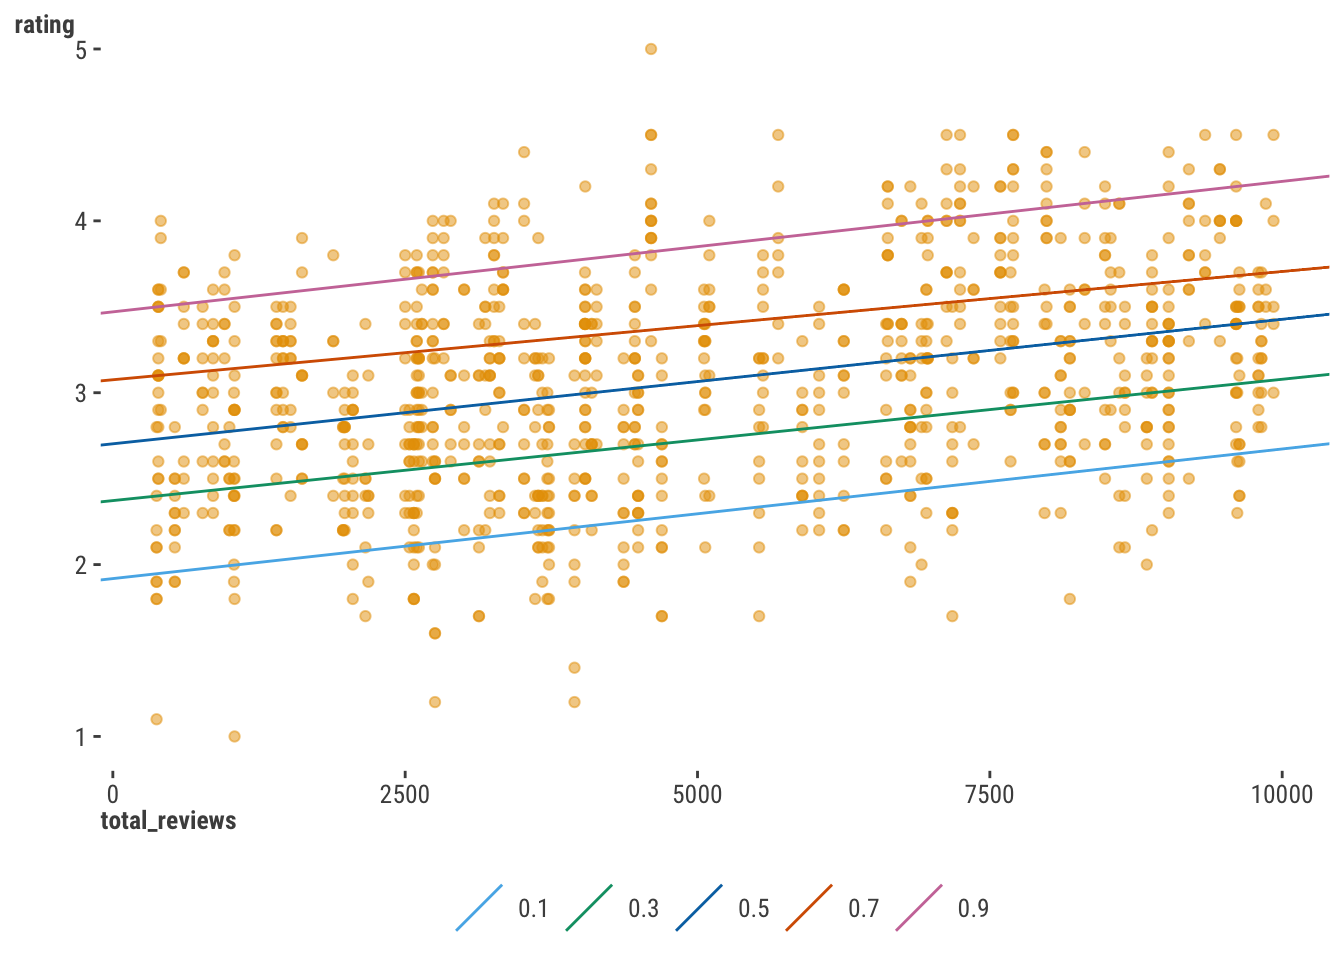
\includegraphics{linear_model_extensions_files/figure-pdf/quantile_lines-1.pdf}

}

\caption{Quantile regression lines}

\end{figure}

Instead of a single model to capture the trend through the mean of the
data, we can now examine the trends within 5 different quantiles of the
data (we aren't limited to just those quantiles, though, and you can
examine any of them that you might find interesting). If we had to put
some words to our visualization, we could say that all of the quantiles
show a positive relationship. While they all appear to have roughly the
same slope, it appears that the 90th quantile has a slightly steeper
slope than the other quantiles, if only modestly so.

\subsection{Quantile Loss Function}\label{quantile-loss-function}

Now that we know how to use standard functions for quantile regression,
let's see one way that we can create a least squares loss function for
fitting a linear regression model and compare it with a function for
quantile loss.

\subsubsection{R}

\begin{Shaded}
\begin{Highlighting}[]
\NormalTok{least\_squares\_loss }\OtherTok{\textless{}{-}} \ControlFlowTok{function}\NormalTok{(par, X, y) \{}
  
\NormalTok{  linear\_parameters }\OtherTok{\textless{}{-}}\NormalTok{ X }\SpecialCharTok{\%*\%}\NormalTok{ par}
  
\NormalTok{  mu }\OtherTok{\textless{}{-}}\NormalTok{ linear\_parameters   }
  
\NormalTok{  loss }\OtherTok{\textless{}{-}} \FunctionTok{crossprod}\NormalTok{(y }\SpecialCharTok{{-}}\NormalTok{ mu)}
\NormalTok{\}}
\end{Highlighting}
\end{Shaded}

\begin{Shaded}
\begin{Highlighting}[]
\NormalTok{quantile\_loss }\OtherTok{\textless{}{-}} \ControlFlowTok{function}\NormalTok{(par, X, y, tau) \{}
  
\NormalTok{  linear\_parameters }\OtherTok{\textless{}{-}}\NormalTok{ X }\SpecialCharTok{\%*\%}\NormalTok{ par}
  
\NormalTok{  residual }\OtherTok{\textless{}{-}}\NormalTok{ y }\SpecialCharTok{{-}}\NormalTok{ linear\_parameters}
  
\NormalTok{  loss }\OtherTok{\textless{}{-}} \FunctionTok{ifelse}\NormalTok{(residual }\SpecialCharTok{\textless{}} \DecValTok{0}\NormalTok{ , }
\NormalTok{                (}\SpecialCharTok{{-}}\DecValTok{1} \SpecialCharTok{+}\NormalTok{ tau)}\SpecialCharTok{*}\NormalTok{residual, }
\NormalTok{                tau}\SpecialCharTok{*}\NormalTok{residual)}
  
  \FunctionTok{sum}\NormalTok{(loss)}
\NormalTok{\}}
\end{Highlighting}
\end{Shaded}

\subsubsection{Python}

\begin{Shaded}
\begin{Highlighting}[]
\KeywordTok{def}\NormalTok{ least\_squares\_loss(par, X, y):}
\NormalTok{  linear\_parameters }\OperatorTok{=}\NormalTok{ X.dot(par)}
  
\NormalTok{  mu }\OperatorTok{=}\NormalTok{ linear\_parameters}
  
\NormalTok{  loss }\OperatorTok{=}\NormalTok{ np.dot(y }\OperatorTok{{-}}\NormalTok{ mu, y }\OperatorTok{{-}}\NormalTok{ mu)}
  
  \ControlFlowTok{return}\NormalTok{ loss}
\end{Highlighting}
\end{Shaded}

\begin{Shaded}
\begin{Highlighting}[]
\KeywordTok{def}\NormalTok{ quantile\_loss(par, X, y, tau):}
\NormalTok{  linear\_parameters }\OperatorTok{=}\NormalTok{ X.dot(par)}
  
\NormalTok{  residual }\OperatorTok{=}\NormalTok{ y }\OperatorTok{{-}}\NormalTok{ linear\_parameters}
  
\NormalTok{  loss }\OperatorTok{=}\NormalTok{ []}

  \ControlFlowTok{for}\NormalTok{ i }\KeywordTok{in}\NormalTok{ residual:}
    \ControlFlowTok{if}\NormalTok{ i }\OperatorTok{\textless{}} \DecValTok{0}\NormalTok{: loss.append((}\OperatorTok{{-}}\DecValTok{1} \OperatorTok{+}\NormalTok{ tau)}\OperatorTok{*}\NormalTok{i)}
    \ControlFlowTok{else}\NormalTok{: loss.append(tau}\OperatorTok{*}\NormalTok{i)}
  
  \ControlFlowTok{return} \BuiltInTok{sum}\NormalTok{(loss)}
\end{Highlighting}
\end{Shaded}

You'll notice right away that we have a few differences. Our quantile
loss function includes the \textbf{tau} argument, which will let us set
our quantile of interest; naturally, it can be any value between 0 and
1. The residual is multiplied by the tau value, only if the residual is
greater than 0. If the residual is negative, we need to add tau to -1.
Since we need a positive value for our loss values, we will multiply our
negative residuals by the negative value produced from -1 plus our tau
value. After that, we just sum all of those positive loss values and do
our best to minimize that summed value.

\subsection{Model Fitting}\label{model-fitting-2}

Now that we have our data and our loss function, we can fit the model
almost exactly like our standard linear model. Again, note the
difference here with our tau value, which we've set to .5 to represent
the median.

\subsubsection{R}

\begin{Shaded}
\begin{Highlighting}[]
\FunctionTok{optim}\NormalTok{(}
  \AttributeTok{par =} \FunctionTok{c}\NormalTok{(}\AttributeTok{intercept =} \DecValTok{0}\NormalTok{, }\AttributeTok{total\_reviews =} \DecValTok{0}\NormalTok{),}
  \AttributeTok{fn  =}\NormalTok{ quantile\_loss,}
  \AttributeTok{X   =}\NormalTok{ X,}
  \AttributeTok{y   =}\NormalTok{ y,}
  \AttributeTok{tau =}\NormalTok{ .}\DecValTok{5}
\NormalTok{)}\SpecialCharTok{$}\NormalTok{par}
\end{Highlighting}
\end{Shaded}

\begin{verbatim}
    intercept total_reviews 
 2.702730e+00  7.258694e-05 
\end{verbatim}

\subsubsection{Python}

\begin{Shaded}
\begin{Highlighting}[]
\ImportTok{from}\NormalTok{ scipy.optimize }\ImportTok{import}\NormalTok{ minimize}

\NormalTok{minimize(}
\NormalTok{  quantile\_loss, }
\NormalTok{  x0 }\OperatorTok{=}\NormalTok{ np.array([}\DecValTok{0}\NormalTok{, }\DecValTok{0}\NormalTok{]), }
\NormalTok{  args }\OperatorTok{=}\NormalTok{ (X, y, }\FloatTok{.5}\NormalTok{)}
\NormalTok{  ).x}
\end{Highlighting}
\end{Shaded}

\begin{verbatim}
array([2.70270449e+00, 7.26658864e-05])
\end{verbatim}

\section{Additive Models}\label{additive-models}

\begin{quote}
Wiggle, wiggle, wiggle, yeah! -- LMFAO
\end{quote}

\subsection{Why Should You Care?}\label{why-should-you-care-3}

Not every relationship is linear and not every relationship is
monotonic. Sometimes, you need to be able to model a relationship that
has a fair amount of nonlinearity -- they can appear as slight curves,
waves, and any other type of wiggle that you can imagine. Additive
models will give you the ability to model those nonlinear relationships
between your features and target.

\subsection{When Straight Lines Aren't
Enough}\label{when-straight-lines-arent-enough}

Fitting a line through your data is always going to be useful,
regardless of whether you are using the median or the mean. Those lines
give us a wonderful ability to say important things about the
relationships between variables and how one variable might influence
another. What if we just want to dispense with the notion that we need
to fit a straight line through some mass of the data? What if we relax
the idea that we need a straight line and think in terms of fitting
something curvy through the data.

In other words, we can go from the straight line in
Figure~\ref{fig-regular_linear_line}:

\begin{figure}

{\centering 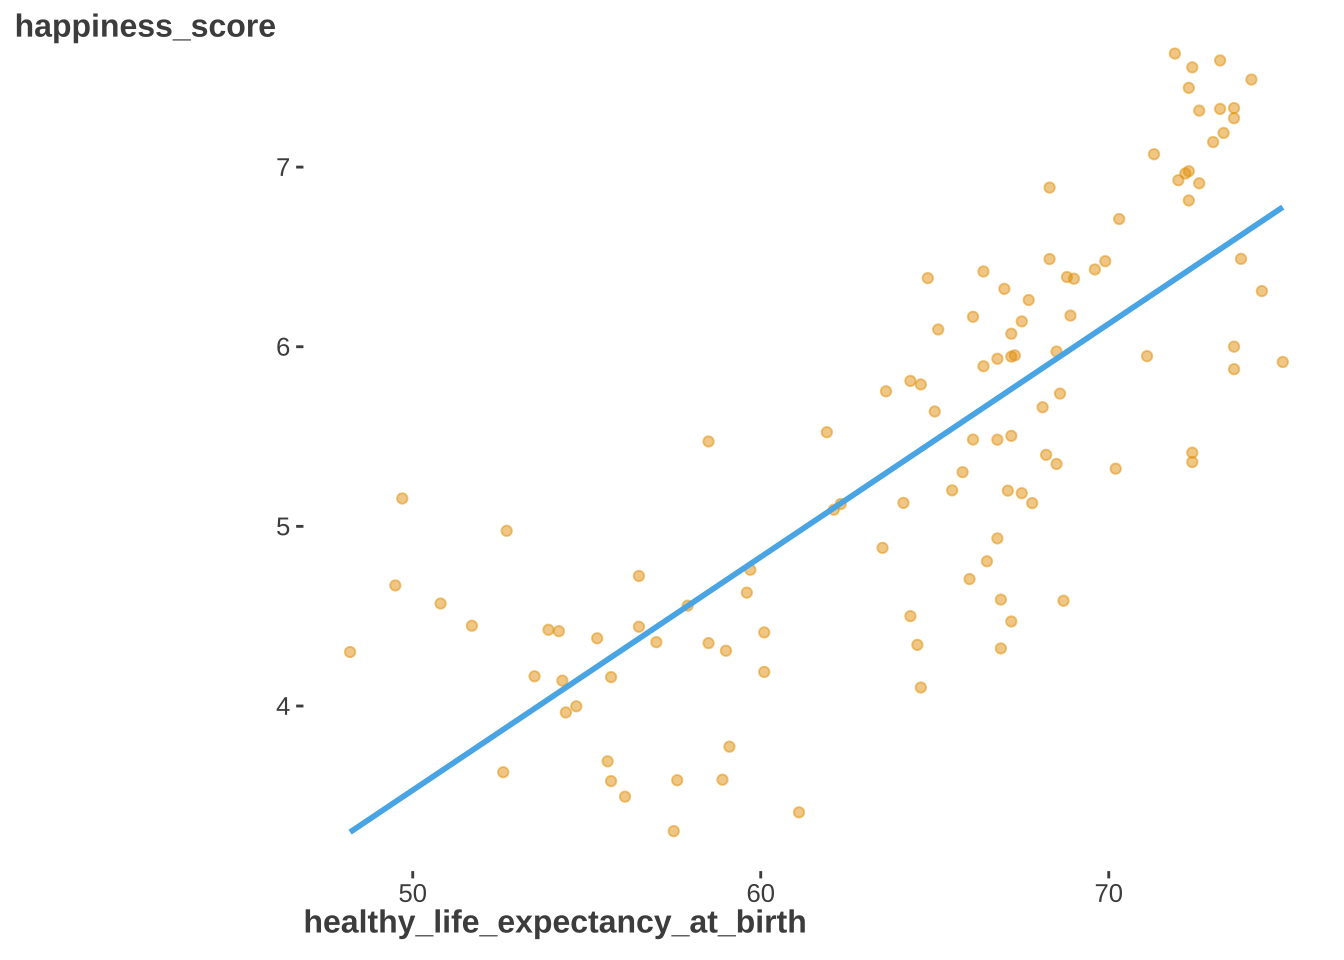
\includegraphics{linear_model_extensions_files/figure-pdf/fig-regular_linear_line-1.pdf}

}

\caption{\label{fig-regular_linear_line}A standard linear model}

\end{figure}

To the curve seen in Figure~\ref{fig-gam_model_line}:

\begin{figure}

{\centering 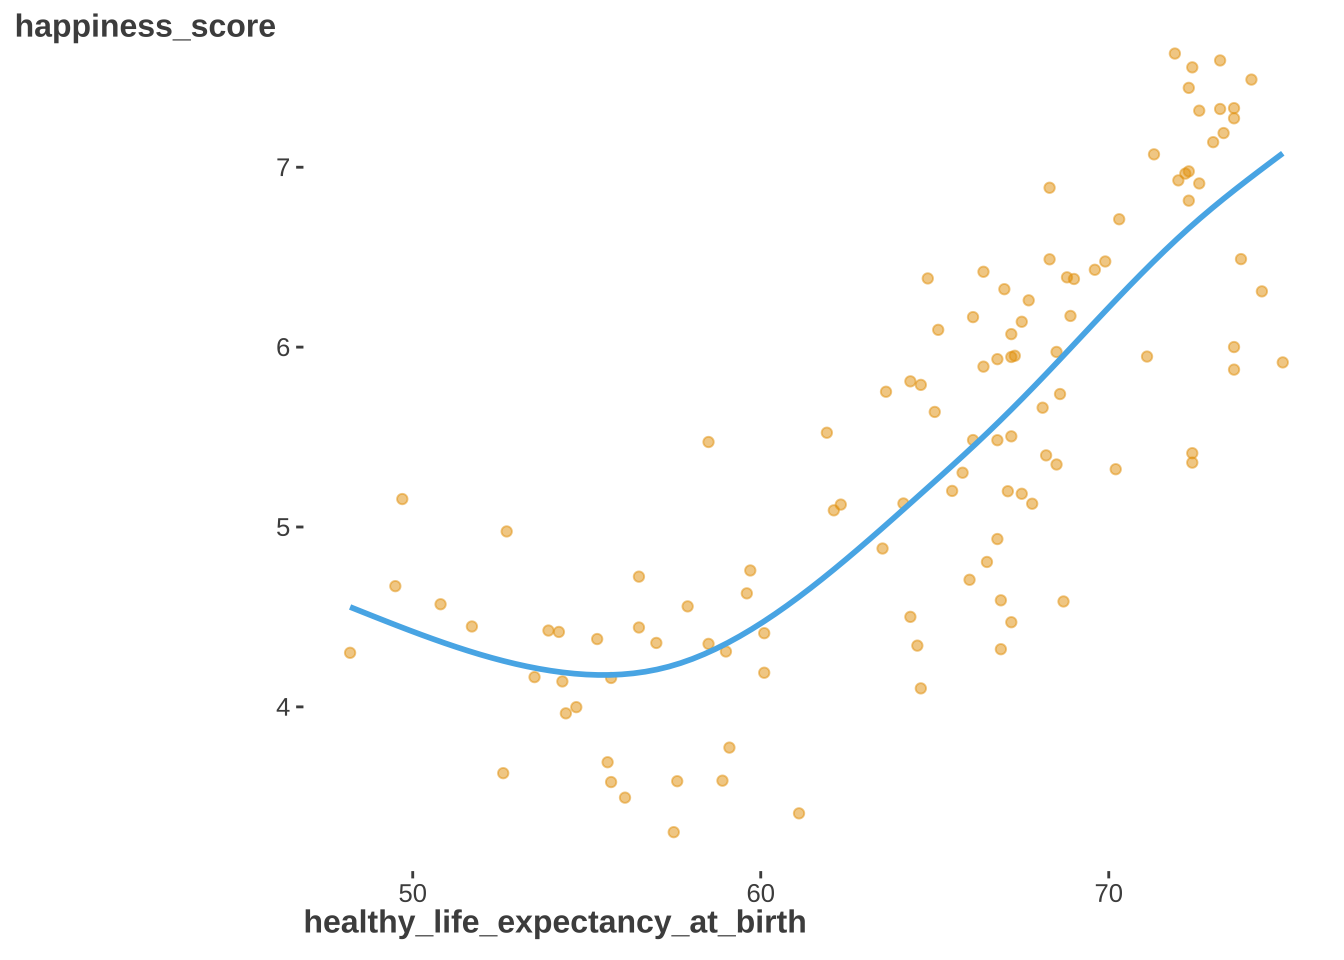
\includegraphics{linear_model_extensions_files/figure-pdf/fig-gam_model_line-1.pdf}

}

\caption{\label{fig-gam_model_line}A generalized additive model}

\end{figure}

That curved line in Figure~\ref{fig-gam_model_line} is called a spline.
Oddly enough, we can still use a linear model to fit this spline through
the data. While this might not give us the same tidy explanation that a
typical line would offer, we will certainly get better prediction.

These models belong to a broad group of \emph{generalized additive
models}, often shortened to GAMs. When we fit a quantile regression, we
made a slight tweak to the \emph{y}; to fit a GAM, we are going to tweak
our predictors. How are we going to tweak them, you might ask? We are
essentially going to let them be an \emph{additive} function of
features. We will have a model that looks like this:

\[
y = f(x) + \epsilon
\]

These additive features have no concern about linearity with the outcome
and will capture nonlinearities in our data very nicely. At this point,
you might be asking yourself, ``Couldn't I just use some type of
polynomial regression or even a nonlinear regression?'' Of course you
could, but both have pretty serious limitations. The typical polynomial
regression likely doesn't fit beyond the data that you currently have
and \textbf{you} are forcing curves to fit through the data. To use a
nonlinear model, you need to know what the underlying nonlinear form
actually looks like before you can even specify the model. A GAM will do
away with both of these issues; it will produce a curve that will best
fit through the data, without the need to know the underlying linear
form.

\subsection{Standard Functions}\label{standard-functions-3}

Now that you have some background, let's use the \texttt{mgcv} package
in R and the \texttt{pygam} package in Python to fit a GAM.

\subsubsection{R}

\begin{Shaded}
\begin{Highlighting}[]
\FunctionTok{library}\NormalTok{(mgcv)}

\NormalTok{gam\_model }\OtherTok{\textless{}{-}} \FunctionTok{gam}\NormalTok{(rating }\SpecialCharTok{\textasciitilde{}} \FunctionTok{s}\NormalTok{(total\_reviews\_sc, }\AttributeTok{bs =} \StringTok{"cr"}\NormalTok{), }\AttributeTok{data =}\NormalTok{ reviews)}

\FunctionTok{summary}\NormalTok{(gam\_model)}
\end{Highlighting}
\end{Shaded}

\begin{verbatim}

Family: gaussian 
Link function: identity 

Formula:
rating ~ s(total_reviews_sc, bs = "cr")

Parametric coefficients:
            Estimate Std. Error t value Pr(>|t|)    
(Intercept)  3.05140    0.01862   163.9   <2e-16 ***
---
Signif. codes:  0 '***' 0.001 '**' 0.01 '*' 0.05 '.' 0.1 ' ' 1

Approximate significance of smooth terms:
                      edf Ref.df    F p-value    
s(total_reviews_sc) 8.672  8.966 16.2  <2e-16 ***
---
Signif. codes:  0 '***' 0.001 '**' 0.01 '*' 0.05 '.' 0.1 ' ' 1

R-sq.(adj) =  0.124   Deviance explained = 13.1%
GCV = 0.34994  Scale est. = 0.34655   n = 1000
\end{verbatim}

\subsubsection{Python}

\begin{Shaded}
\begin{Highlighting}[]
\ImportTok{from}\NormalTok{ pygam }\ImportTok{import}\NormalTok{ LinearGAM, s}

\NormalTok{y }\OperatorTok{=}\NormalTok{ reviews[}\StringTok{\textquotesingle{}rating\textquotesingle{}}\NormalTok{]}

\NormalTok{X }\OperatorTok{=}\NormalTok{ pd.DataFrame(}
\NormalTok{  \{}\StringTok{\textquotesingle{}intercept\textquotesingle{}}\NormalTok{: }\DecValTok{1}\NormalTok{, }
  \StringTok{\textquotesingle{}total\_reviews\textquotesingle{}}\NormalTok{: reviews[}\StringTok{\textquotesingle{}total\_reviews\textquotesingle{}}\NormalTok{]\}}
\NormalTok{)}

\NormalTok{gam\_model }\OperatorTok{=}\NormalTok{ LinearGAM(s(}\DecValTok{0}\NormalTok{)).fit(X, y)}

\NormalTok{gam\_model.summary()}
\end{Highlighting}
\end{Shaded}

\begin{verbatim}
LinearGAM                                                                                                 
=============================================== ==========================================================
Distribution:                        NormalDist Effective DoF:                                         1.0
Link Function:                     IdentityLink Log Likelihood:                                 -1254.3233
Number of Samples:                         1000 AIC:                                             2512.6465
                                                AICc:                                            2512.6585
                                                GCV:                                                0.3962
                                                Scale:                                              0.3955
                                                Pseudo R-Squared:                                      0.0
==========================================================================================================
Feature Function                  Lambda               Rank         EDoF         P > x        Sig. Code   
================================= ==================== ============ ============ ============ ============
s(0)                              [0.6]                20           1.0          1.11e-16     ***         
intercept                                              1            0.0          1.11e-16     ***         
==========================================================================================================
Significance codes:  0 '***' 0.001 '**' 0.01 '*' 0.05 '.' 0.1 ' ' 1

WARNING: Fitting splines and a linear function to a feature introduces a model identifiability problem
         which can cause p-values to appear significant when they are not.

WARNING: p-values calculated in this manner behave correctly for un-penalized models or models with
         known smoothing parameters, but when smoothing parameters have been estimated, the p-values
         are typically lower than they should be, meaning that the tests reject the null too readily.
\end{verbatim}

For the results of our gam model, one of the best places to look first
is the \texttt{edf} column. The \texttt{edf} column is the
\emph{effective degrees of freedom}. You can think of \texttt{edf} as a
measure of wiggle in the relationship between the predictor and the
target. The higher the \texttt{edf}, the more wiggle you have. If you
have a value close to 1, then you have a linear relationship. With an
\texttt{edf} of 8.672, we can be pretty confident that a nonlinear
relationship gives a better idea about the relationship between
\texttt{total\_reviews} and \texttt{rating} than a linear relationship.

We also get information about our Adjusted \(R^2\) (\textbf{R-sq.(adj)})
and \textbf{Deviance explained}, which is an analog to the unadjusted
\(R^2\) value for a Gaussian model. We also have \textbf{GCV} -- the
generalized cross validation score. It is an estimate of the mean square
prediction error based on a leave-one-out cross validation estimation
process. Naturally, the lower the GCV, the better the model.

\subsection{Splines}\label{splines}

Now that you've gotten a taste of a standard way of specifying a GAM,
let's roll our own. We are going to need to generate several functions
to make this work. The first will be to produce the \emph{cubic spline}.
Do take note that there are many different types of splines that could
be used.

\subsubsection{R}

\begin{Shaded}
\begin{Highlighting}[]
\NormalTok{cubic\_spline }\OtherTok{\textless{}{-}} \ControlFlowTok{function}\NormalTok{(x, z) \{}
\NormalTok{  ((z }\SpecialCharTok{{-}} \FloatTok{0.5}\NormalTok{)}\SpecialCharTok{\^{}}\DecValTok{2} \SpecialCharTok{{-}} \DecValTok{1}\SpecialCharTok{/}\DecValTok{12}\NormalTok{) }\SpecialCharTok{*}\NormalTok{ ((x }\SpecialCharTok{{-}} \FloatTok{0.5}\NormalTok{)}\SpecialCharTok{\^{}}\DecValTok{2} \SpecialCharTok{{-}} \DecValTok{1}\SpecialCharTok{/}\DecValTok{12}\NormalTok{)}\SpecialCharTok{/}\DecValTok{4} \SpecialCharTok{{-}}
\NormalTok{    ((}\FunctionTok{abs}\NormalTok{(x }\SpecialCharTok{{-}}\NormalTok{ z) }\SpecialCharTok{{-}} \FloatTok{0.5}\NormalTok{)}\SpecialCharTok{\^{}}\DecValTok{4} \SpecialCharTok{{-}}\NormalTok{ (}\FunctionTok{abs}\NormalTok{(x }\SpecialCharTok{{-}}\NormalTok{ z) }\SpecialCharTok{{-}} \FloatTok{0.5}\NormalTok{)}\SpecialCharTok{\^{}}\DecValTok{2} \SpecialCharTok{/} \DecValTok{2} \SpecialCharTok{+} \DecValTok{7}\SpecialCharTok{/}\DecValTok{240}\NormalTok{) }\SpecialCharTok{/} \DecValTok{24}
\NormalTok{\}}
\end{Highlighting}
\end{Shaded}

\subsubsection{Python}

\begin{Shaded}
\begin{Highlighting}[]
\ImportTok{import}\NormalTok{ numpy }\ImportTok{as}\NormalTok{ np}

\KeywordTok{def}\NormalTok{ cubic\_spline(x,z):}
    \ControlFlowTok{return}\NormalTok{ (((z }\OperatorTok{{-}} \FloatTok{0.5}\NormalTok{)}\OperatorTok{**}\DecValTok{2} \OperatorTok{{-}} \DecValTok{1}\OperatorTok{/}\DecValTok{12}\NormalTok{) }\OperatorTok{*}\NormalTok{ ((x }\OperatorTok{{-}} \FloatTok{0.5}\NormalTok{)}\OperatorTok{**}\DecValTok{2} \OperatorTok{{-}} \DecValTok{1}\OperatorTok{/}\DecValTok{12}\NormalTok{)}\OperatorTok{/}\DecValTok{4} \OperatorTok{{-}}
\NormalTok{            ((np.}\BuiltInTok{abs}\NormalTok{(x }\OperatorTok{{-}}\NormalTok{ z) }\OperatorTok{{-}} \FloatTok{0.5}\NormalTok{)}\OperatorTok{**}\DecValTok{4} \OperatorTok{{-}}\NormalTok{ (np.}\BuiltInTok{abs}\NormalTok{(x }\OperatorTok{{-}}\NormalTok{ z) }\OperatorTok{{-}} \FloatTok{0.5}\NormalTok{)}\OperatorTok{**}\DecValTok{2} \OperatorTok{/} \DecValTok{2} \OperatorTok{+} \DecValTok{7}\OperatorTok{/}\DecValTok{240}\NormalTok{) }\OperatorTok{/} \DecValTok{24}\NormalTok{)}
\end{Highlighting}
\end{Shaded}

\subsection{Model Matrix Function}\label{model-matrix-function}

Then we a function to produce the model matrix:

\subsubsection{R}

\begin{Shaded}
\begin{Highlighting}[]
\NormalTok{splX }\OtherTok{\textless{}{-}} \ControlFlowTok{function}\NormalTok{(x, knots) \{}
\NormalTok{  q }\OtherTok{\textless{}{-}} \FunctionTok{length}\NormalTok{(knots) }\SpecialCharTok{+} \DecValTok{2}        \CommentTok{\# number of parameters}
\NormalTok{  n }\OtherTok{\textless{}{-}} \FunctionTok{length}\NormalTok{(x)                }\CommentTok{\# number of observations}
\NormalTok{  X }\OtherTok{\textless{}{-}} \FunctionTok{matrix}\NormalTok{(}\DecValTok{1}\NormalTok{, n, q)          }\CommentTok{\# initialized model matrix}
\NormalTok{  X[ ,}\DecValTok{2}\NormalTok{] }\OtherTok{\textless{}{-}}\NormalTok{ x                   }\CommentTok{\# set second column to x}
\NormalTok{  X[ ,}\DecValTok{3}\SpecialCharTok{:}\NormalTok{q] }\OtherTok{\textless{}{-}} \FunctionTok{outer}\NormalTok{(x, knots, }\AttributeTok{FUN =}\NormalTok{ cubic\_spline) }
\NormalTok{  X}
\NormalTok{\}}
\end{Highlighting}
\end{Shaded}

\subsubsection{Python}

\begin{Shaded}
\begin{Highlighting}[]
\KeywordTok{def}\NormalTok{ splX(x, knots):}
\NormalTok{    q }\OperatorTok{=} \BuiltInTok{len}\NormalTok{(knots) }\OperatorTok{+} \DecValTok{2}
\NormalTok{    n }\OperatorTok{=} \BuiltInTok{len}\NormalTok{(x)}
\NormalTok{    X }\OperatorTok{=}\NormalTok{ np.ones((n, q))}
\NormalTok{    X[:,}\DecValTok{1}\NormalTok{] }\OperatorTok{=}\NormalTok{ x}
    \ControlFlowTok{for}\NormalTok{ i }\KeywordTok{in} \BuiltInTok{range}\NormalTok{(}\DecValTok{2}\NormalTok{, q):}
\NormalTok{        X[:,i] }\OperatorTok{=}\NormalTok{ cubic\_spline(x, knots[i}\OperatorTok{{-}}\DecValTok{2}\NormalTok{])}
    \ControlFlowTok{return}\NormalTok{ X}
\end{Highlighting}
\end{Shaded}

This model matrix will help us to produce an \emph{unpenalized spline}.

\subsection{Model Matrix}\label{model-matrix}

We can create a model with 4 knots -- you can think of knots as places
where individual regression lines will get joined together. You can
always experiment with more or less knots. Once we have our knots ready,
we can create the model matrix.

As soon as you create your \texttt{X} object, you should take a look at
it. It will be a matrix with 4 columns. The first column will be all 1s,
the second column will be the scaled \texttt{user\_age}, and the last
two columns will be the cubic splines.

\subsubsection{R}

\begin{Shaded}
\begin{Highlighting}[]
\NormalTok{knots }\OtherTok{\textless{}{-}} \DecValTok{1}\SpecialCharTok{:}\DecValTok{4}\SpecialCharTok{/}\DecValTok{5}
\end{Highlighting}
\end{Shaded}

\begin{Shaded}
\begin{Highlighting}[]
\NormalTok{rating }\OtherTok{\textless{}{-}}\NormalTok{ reviews}\SpecialCharTok{$}\NormalTok{rating}

\NormalTok{x }\OtherTok{\textless{}{-}}\NormalTok{ reviews}\SpecialCharTok{$}\NormalTok{total\_reviews}

\NormalTok{X }\OtherTok{\textless{}{-}} \FunctionTok{splX}\NormalTok{(x, knots)            }
\end{Highlighting}
\end{Shaded}

\begin{Shaded}
\begin{Highlighting}[]
\FunctionTok{head}\NormalTok{(X)}
\end{Highlighting}
\end{Shaded}

\begin{verbatim}
     [,1] [,2]          [,3]          [,4]          [,5]          [,6]
[1,]    1 2574 -1.827050e+12 -1.826482e+12 -1.825914e+12 -1.825346e+12
[2,]    1 7590 -1.382279e+14 -1.382133e+14 -1.381987e+14 -1.381842e+14
[3,]    1 1618 -2.850697e+11 -2.849287e+11 -2.847878e+11 -2.846469e+11
[4,]    1 6251 -6.359049e+13 -6.358236e+13 -6.357422e+13 -6.356608e+13
[5,]    1 6040 -5.542876e+13 -5.542142e+13 -5.541408e+13 -5.540674e+13
[6,]    1 7130 -1.076407e+14 -1.076286e+14 -1.076165e+14 -1.076044e+14
\end{verbatim}

\subsubsection{Python}

\begin{Shaded}
\begin{Highlighting}[]
\NormalTok{knots }\OperatorTok{=}\NormalTok{ np.arange(}\DecValTok{1}\NormalTok{, }\DecValTok{5}\NormalTok{) }\OperatorTok{/} \DecValTok{5}
\end{Highlighting}
\end{Shaded}

\begin{Shaded}
\begin{Highlighting}[]
\NormalTok{x }\OperatorTok{=}\NormalTok{ reviews[}\StringTok{\textquotesingle{}total\_reviews\textquotesingle{}}\NormalTok{]}

\NormalTok{rating }\OperatorTok{=}\NormalTok{ reviews[}\StringTok{\textquotesingle{}rating\textquotesingle{}}\NormalTok{]}

\NormalTok{X }\OperatorTok{=}\NormalTok{ splX(x, knots)}
\end{Highlighting}
\end{Shaded}

\begin{Shaded}
\begin{Highlighting}[]
\NormalTok{X[:}\DecValTok{5}\NormalTok{,:]}
\end{Highlighting}
\end{Shaded}

\begin{verbatim}
array([[ 1.00000000e+00,  2.57400000e+03, -1.82704987e+12,
        -1.82648207e+12, -1.82591427e+12, -1.82534646e+12],
       [ 1.00000000e+00,  7.59000000e+03, -1.38227877e+14,
        -1.38213307e+14, -1.38198738e+14, -1.38184169e+14],
       [ 1.00000000e+00,  1.61800000e+03, -2.85069671e+11,
        -2.84928740e+11, -2.84787808e+11, -2.84646876e+11],
       [ 1.00000000e+00,  6.25100000e+03, -6.35904948e+13,
        -6.35823568e+13, -6.35742188e+13, -6.35660807e+13],
       [ 1.00000000e+00,  6.04000000e+03, -5.54287604e+13,
        -5.54214191e+13, -5.54140778e+13, -5.54067364e+13]])
\end{verbatim}

\subsection{Model Fitting}\label{model-fitting-3}

Now that we have a model matrix, \texttt{X}, we can fit the model. All
of the hardwork was done in creating the model matrix and we can just
use \texttt{lm} or \texttt{OLS} to fit the model.

\subsubsection{R}

\begin{Shaded}
\begin{Highlighting}[]
\NormalTok{fit\_lm }\OtherTok{\textless{}{-}} \FunctionTok{lm}\NormalTok{(rating }\SpecialCharTok{\textasciitilde{}}\NormalTok{ X)}

\NormalTok{fit\_lm}
\end{Highlighting}
\end{Shaded}

\begin{verbatim}

Call:
lm(formula = rating ~ X)

Coefficients:
(Intercept)           X1           X2           X3           X4           X5           X6  
  2.826e+00           NA   -8.055e-06   -9.670e-11    9.670e-11           NA           NA  
\end{verbatim}

\subsubsection{Python}

\begin{Shaded}
\begin{Highlighting}[]
\ImportTok{import}\NormalTok{ statsmodels.api }\ImportTok{as}\NormalTok{ sm}

\NormalTok{fit\_lm }\OperatorTok{=}\NormalTok{ sm.OLS(rating, X).fit()}

\NormalTok{fit\_lm.summary()}
\end{Highlighting}
\end{Shaded}

\begin{verbatim}
<class 'statsmodels.iolib.summary.Summary'>
"""
                            OLS Regression Results                            
==============================================================================
Dep. Variable:                 rating   R-squared:                      -1.346
Model:                            OLS   Adj. R-squared:                 -1.351
Method:                 Least Squares   F-statistic:                    -286.0
Date:                Sat, 09 Dec 2023   Prob (F-statistic):               1.00
Time:                        10:38:17   Log-Likelihood:                -1381.0
No. Observations:                1000   AIC:                             2768.
Df Residuals:                     997   BIC:                             2783.
Df Model:                           2                                         
Covariance Type:            nonrobust                                         
==============================================================================
                 coef    std err          t      P>|t|      [0.025      0.975]
------------------------------------------------------------------------------
const       5.439e-07   1.07e-08     51.027      0.000    5.23e-07    5.65e-07
x1             0.0012   2.42e-05     51.027      0.000       0.001       0.001
x2          1.186e-05   2.32e-07     51.025      0.000    1.14e-05    1.23e-05
x3         -1.089e-05   2.13e-07    -51.027      0.000   -1.13e-05   -1.05e-05
x4         -1.381e-05   2.71e-07    -51.026      0.000   -1.43e-05   -1.33e-05
x5          1.284e-05   2.52e-07     51.028      0.000    1.23e-05    1.33e-05
==============================================================================
Omnibus:                       64.602   Durbin-Watson:                   1.992
Prob(Omnibus):                  0.000   Jarque-Bera (JB):               75.828
Skew:                           0.644   Prob(JB):                     3.42e-17
Kurtosis:                       3.404   Cond. No.                     1.27e+16
==============================================================================

Notes:
[1] Standard Errors assume that the covariance matrix of the errors is correctly specified.
[2] The condition number is large, 1.27e+16. This might indicate that there are
strong multicollinearity or other numerical problems.
"""
\end{verbatim}

\subsection{Prediction}\label{prediction-1}

We can set some prediction values for this model:

\subsubsection{R}

\begin{Shaded}
\begin{Highlighting}[]
\NormalTok{xp }\OtherTok{\textless{}{-}} \FunctionTok{seq}\NormalTok{(}\DecValTok{0}\NormalTok{, }\DecValTok{1}\NormalTok{, }\AttributeTok{by =}\NormalTok{ .}\DecValTok{01}\NormalTok{)}
\NormalTok{Xp }\OtherTok{\textless{}{-}} \FunctionTok{splX}\NormalTok{(xp, knots)  }
\end{Highlighting}
\end{Shaded}

\subsubsection{Python}

\begin{Shaded}
\begin{Highlighting}[]
\NormalTok{xp }\OperatorTok{=}\NormalTok{ np.arange(}\DecValTok{0}\NormalTok{, }\DecValTok{1}\NormalTok{, }\FloatTok{0.01}\NormalTok{)}
\NormalTok{Xp }\OperatorTok{=}\NormalTok{ splX(xp, knots)}
\end{Highlighting}
\end{Shaded}

While creating those predictions is nice, using them to visualize the
model is far more helpful.

\begin{figure}

{\centering 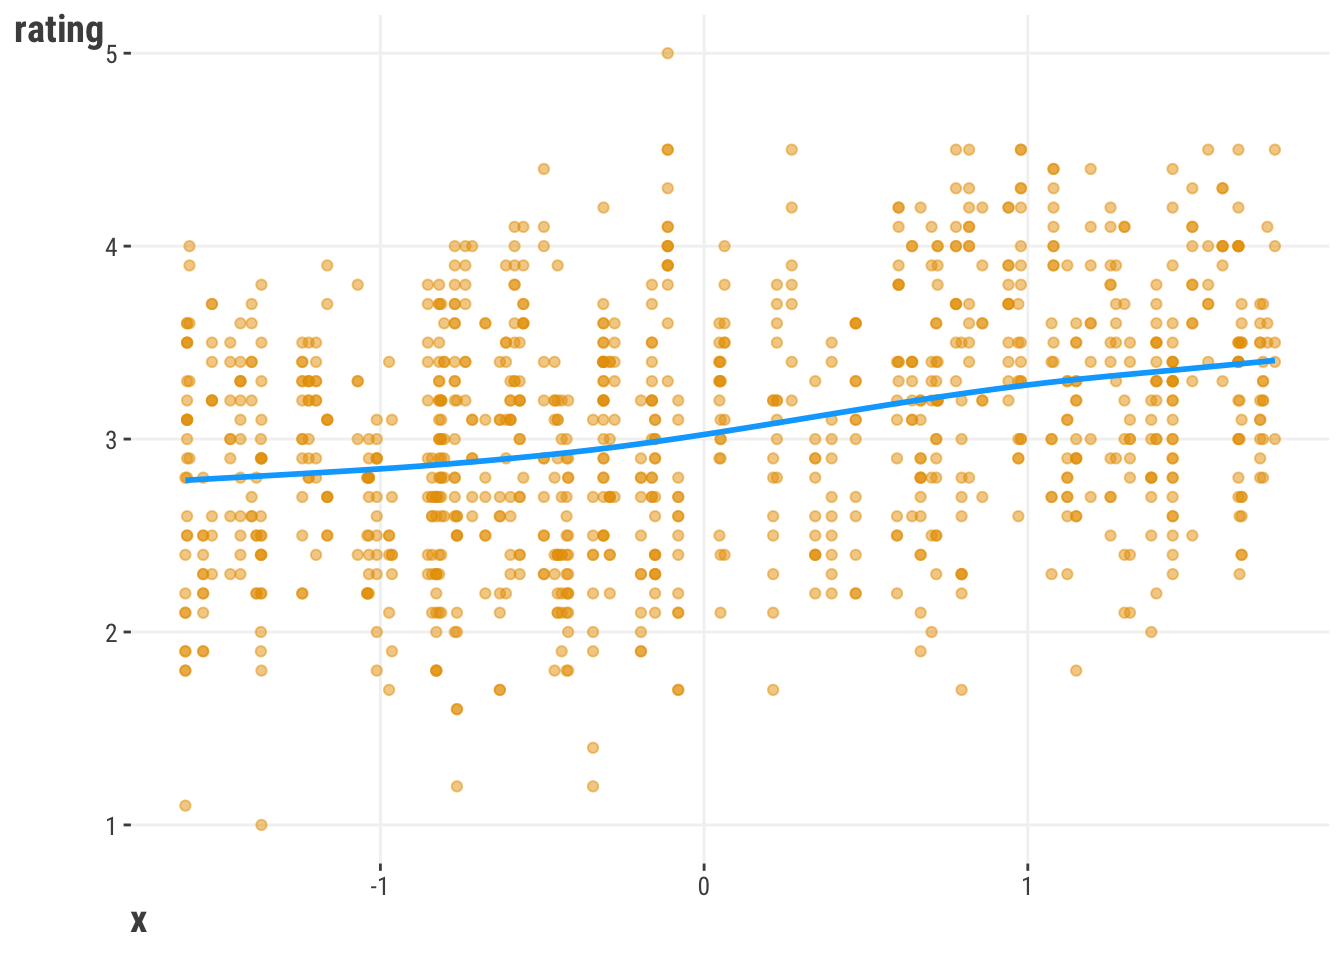
\includegraphics{linear_model_extensions_files/figure-pdf/fig-spline_viz-1.pdf}

}

\caption{\label{fig-spline_viz}Visualizing cubic regression spline}

\end{figure}

In Figure~\ref{fig-spline_viz}, we can see that the relationship starts
a bit flat, increases, and then flattens out again. This is a pretty
good example of a nonlinear relationship.

\subsection{Penalized Cubic Spline}\label{penalized-cubic-spline}

Recall that this is an unpenalized cubic spline. If we want to have a
finer degree of control over that wiggly line, we can include a
\textbf{lambda penalty}.

We'll need to change up our spline function just a bit.

\subsubsection{R}

\begin{Shaded}
\begin{Highlighting}[]
\NormalTok{splS }\OtherTok{\textless{}{-}} \ControlFlowTok{function}\NormalTok{(knots) \{}
\NormalTok{  q }\OtherTok{\textless{}{-}} \FunctionTok{length}\NormalTok{(knots) }\SpecialCharTok{+} \DecValTok{2}
\NormalTok{  S }\OtherTok{\textless{}{-}} \FunctionTok{matrix}\NormalTok{(}\DecValTok{0}\NormalTok{, q, q) }
\NormalTok{  S[}\DecValTok{3}\SpecialCharTok{:}\NormalTok{q, }\DecValTok{3}\SpecialCharTok{:}\NormalTok{q] }\OtherTok{\textless{}{-}} \FunctionTok{outer}\NormalTok{(knots, knots, }\AttributeTok{FUN =}\NormalTok{ cubic\_spline)}
\NormalTok{  S}
\NormalTok{\}}
\end{Highlighting}
\end{Shaded}

\subsubsection{Python}

\begin{Shaded}
\begin{Highlighting}[]
\KeywordTok{def}\NormalTok{ splS(knots):}
\NormalTok{    q }\OperatorTok{=} \BuiltInTok{len}\NormalTok{(knots) }\OperatorTok{+} \DecValTok{2}
\NormalTok{    S }\OperatorTok{=}\NormalTok{ np.zeros((q, q))}
\NormalTok{    S[}\DecValTok{2}\NormalTok{:, }\DecValTok{2}\NormalTok{:] }\OperatorTok{=}\NormalTok{ cubic\_spline(knots, knots[:,}\VariableTok{None}\NormalTok{])}
    \ControlFlowTok{return}\NormalTok{ S}
\end{Highlighting}
\end{Shaded}

We also need to be able to take the square root of our entire matrix.
This is a bit more complicated than it sounds. We need to take the
eigenvalue decomposition of the matrix, take the square root of the
eigenvalues, and then recombine the matrix.

\subsubsection{R}

\begin{Shaded}
\begin{Highlighting}[]
\NormalTok{mat\_sqrt }\OtherTok{\textless{}{-}} \ControlFlowTok{function}\NormalTok{(S) \{}
\NormalTok{  d }\OtherTok{\textless{}{-}} \FunctionTok{eigen}\NormalTok{(S, }\AttributeTok{symmetric =} \ConstantTok{TRUE}\NormalTok{)}
\NormalTok{  rS }\OtherTok{\textless{}{-}}\NormalTok{ d}\SpecialCharTok{$}\NormalTok{vectors }\SpecialCharTok{\%*\%} \FunctionTok{diag}\NormalTok{(d}\SpecialCharTok{$}\NormalTok{values}\SpecialCharTok{\^{}}\NormalTok{.}\DecValTok{5}\NormalTok{) }\SpecialCharTok{\%*\%} \FunctionTok{t}\NormalTok{(d}\SpecialCharTok{$}\NormalTok{vectors)}
\NormalTok{  rS}
\NormalTok{\}}
\end{Highlighting}
\end{Shaded}

\subsubsection{Python}

\begin{Shaded}
\begin{Highlighting}[]
\KeywordTok{def}\NormalTok{ mat\_sqrt(S):}
\NormalTok{    w, v }\OperatorTok{=}\NormalTok{ np.linalg.eig(S)}
\NormalTok{    rS }\OperatorTok{=}\NormalTok{ v }\OperatorTok{@}\NormalTok{ np.diag(w}\OperatorTok{**}\FloatTok{.5}\NormalTok{) }\OperatorTok{@}\NormalTok{ v.T}
    \ControlFlowTok{return}\NormalTok{ rS}
\end{Highlighting}
\end{Shaded}

\subsection{Penalized Model Fitting
Function}\label{penalized-model-fitting-function}

With those functions in hand, we can create the function to fit the
entire model.

\subsubsection{R}

\begin{Shaded}
\begin{Highlighting}[]
\NormalTok{prs\_fit }\OtherTok{\textless{}{-}} \ControlFlowTok{function}\NormalTok{(y, x, knots, lambda) \{}
\NormalTok{  q  }\OtherTok{=} \FunctionTok{length}\NormalTok{(knots) }\SpecialCharTok{+} \DecValTok{2}    \CommentTok{\# dimension of basis}
\NormalTok{  n  }\OtherTok{=} \FunctionTok{length}\NormalTok{(x)            }\CommentTok{\# number of observations}
\NormalTok{  Xa }\OtherTok{=} \FunctionTok{rbind}\NormalTok{(}\FunctionTok{splX}\NormalTok{(x, knots), }\FunctionTok{mat\_sqrt}\NormalTok{(}\FunctionTok{splS}\NormalTok{(knots))}\SpecialCharTok{*}\FunctionTok{sqrt}\NormalTok{(lambda)) }\CommentTok{\# augmented model matrix}
\NormalTok{  y[(n }\SpecialCharTok{+} \DecValTok{1}\NormalTok{)}\SpecialCharTok{:}\NormalTok{(n}\SpecialCharTok{+}\NormalTok{q)] }\OtherTok{=} \DecValTok{0}      \CommentTok{\# augment the data vector}
  
  \FunctionTok{lm}\NormalTok{(y }\SpecialCharTok{\textasciitilde{}}\NormalTok{ Xa }\SpecialCharTok{{-}} \DecValTok{1}\NormalTok{) }\CommentTok{\# fit and return penalized regression spline}
\NormalTok{\}}
\end{Highlighting}
\end{Shaded}

\subsubsection{Python}

\begin{Shaded}
\begin{Highlighting}[]
\KeywordTok{def}\NormalTok{ prs\_fit(y, x, knots, lamba):}
\NormalTok{    q }\OperatorTok{=} \BuiltInTok{len}\NormalTok{(knots) }\OperatorTok{+} \DecValTok{2}
\NormalTok{    n }\OperatorTok{=} \BuiltInTok{len}\NormalTok{(x)}
\NormalTok{    Xa }\OperatorTok{=}\NormalTok{ np.vstack(}
\NormalTok{      (splX(x, knots), mat\_sqrt(splS(knots))}\OperatorTok{*}\NormalTok{np.sqrt(lamba))}
\NormalTok{      )}
\NormalTok{    y\_add }\OperatorTok{=}\NormalTok{ np.zeros(q)}
\NormalTok{    y }\OperatorTok{=}\NormalTok{ y.to\_numpy()}
\NormalTok{    y }\OperatorTok{=}\NormalTok{ np.concatenate((y, y\_add), axis }\OperatorTok{=} \DecValTok{0}\NormalTok{)}
    \ControlFlowTok{return}\NormalTok{ sm.OLS(y, Xa).fit()}
\end{Highlighting}
\end{Shaded}

Notice again that magic happens in the model matrix, but that we are
still just using \texttt{lm} or \texttt{OLS} to fit the model.

\subsection{Penalized Model Fitting}\label{penalized-model-fitting}

Let's stick with 4 knots and see what happens when we set our lambda to
.1:

\subsubsection{R}

\begin{Shaded}
\begin{Highlighting}[]
\NormalTok{knots }\OtherTok{\textless{}{-}} \DecValTok{1}\SpecialCharTok{:}\DecValTok{4}\SpecialCharTok{/}\DecValTok{5}

\NormalTok{fit\_penalized }\OtherTok{\textless{}{-}} \FunctionTok{prs\_fit}\NormalTok{(}
\NormalTok{  y }\OtherTok{\textless{}{-}}\NormalTok{ rating,}
\NormalTok{  x }\OtherTok{\textless{}{-}}\NormalTok{ x,}
\NormalTok{  knots }\OtherTok{\textless{}{-}}\NormalTok{ knots,}
\NormalTok{  lambda }\OtherTok{\textless{}{-}}\NormalTok{ .}\DecValTok{1}
\NormalTok{) }

\NormalTok{Xp }\OtherTok{\textless{}{-}} \FunctionTok{splX}\NormalTok{(xp, knots) }
\end{Highlighting}
\end{Shaded}

\subsubsection{Python}

\begin{Shaded}
\begin{Highlighting}[]
\NormalTok{knots }\OperatorTok{=}\NormalTok{ np.arange(}\DecValTok{1}\NormalTok{, }\DecValTok{5}\NormalTok{)}\OperatorTok{/}\DecValTok{5}

\NormalTok{fit\_penalized }\OperatorTok{=}\NormalTok{ prs\_fit(}
\NormalTok{    y }\OperatorTok{=}\NormalTok{ y,}
\NormalTok{    x }\OperatorTok{=}\NormalTok{ x,}
\NormalTok{    knots }\OperatorTok{=}\NormalTok{ knots,}
\NormalTok{    lamba }\OperatorTok{=} \FloatTok{.1}
\NormalTok{)}

\NormalTok{Xp }\OperatorTok{=}\NormalTok{ splX(xp, knots)}
\end{Highlighting}
\end{Shaded}

As shown in Figure~\ref{fig-r_lambda_1_viz}, there is definitely some
wiggle to that line, but it is not as extreme as what we saw with our
unpenalized cubic spline.

\begin{figure}

{\centering 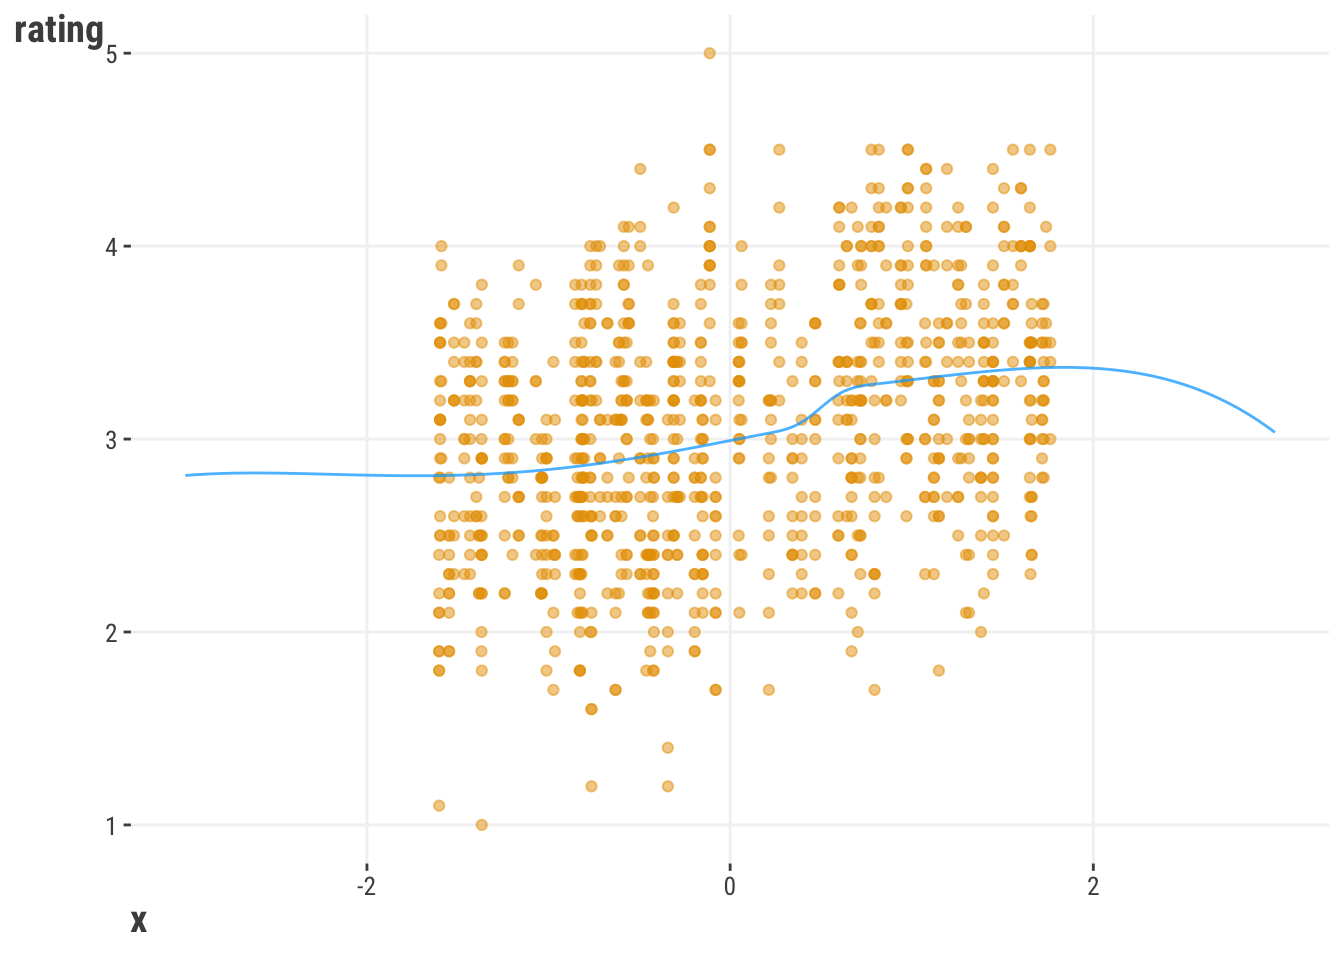
\includegraphics{linear_model_extensions_files/figure-pdf/fig-r_lambda_1_viz-1.pdf}

}

\caption{\label{fig-r_lambda_1_viz}GAM model with lambda set to .1}

\end{figure}

We can test out what happens at different lambda values:

\begin{figure}

{\centering \includegraphics{linear_model_extensions_files/figure-pdf/fig-lambda_value_viz-1.pdf}

}

\caption{\label{fig-lambda_value_viz}GAM model with different lambda
values}

\end{figure}

What can we take from Figure~\ref{fig-lambda_value_viz}? As lambda
values get closer to 1, we see lines that look very similar to a
standard linear model. If you recall the our function to fit the model,
we multiplied the square root of the matrix by the square root of the
lambda value; since the square root of 1 is 1, we wouldn't see anything
too interesting happen. As our lambda value gets lower, we see an
increasing amount of wiggle happen.

Naturally, this is a great time to think about how these models would
work on new data. As lambda gets smaller, we are fitting our in-sample
data much better. How do you think this would fare with unseen data? If
you'd say that we would do well with training and horrible on testing,
we'd likely agree with you.

\section{Mixed Models}\label{mixed-models}

\subsection{Why Should You Care?}\label{why-should-you-care-4}

Structures within your data are important and paying attention to how
data might be grouped in some way will let you generate more insights
about how observations within and between groups might behave. After
all, people working in the same department are likely to have a more
similar experience than people working in a different department. Mixed
models will let us handle nested and grouped data, all while getting the
benefits of a standard linear model.

\subsection{Knowing Your Data}\label{knowing-your-data}

As much fun as modeling is, knowing your data is far more important. You
can throw any model you want at your data, from simple to fancy, but you
can count on disappointment if you don't fundamentally know the
structures that live within your data. Let's take a quick look at the
following visualizations:

\begin{figure}

{\centering \includegraphics{linear_model_extensions_files/figure-pdf/fig-year-release-rating-1.pdf}

}

\caption{\label{fig-year-release-rating}Linear relationship between year
of movie release and rating.}

\end{figure}

In Figure~\ref{fig-year-release-rating}, we see a pretty solid positive
relationship between the total number of reviews and ratings. We could
probably just stop there, but we might be ignoring something substantial
within our data: genre. We might want to ask a question, ``Does this
relationship work the same way across the different genre?''

\begin{figure}

{\centering \includegraphics{linear_model_extensions_files/figure-pdf/fig-year-release-genre-rating-1.pdf}

}

\caption{\label{fig-year-release-genre-rating}Linear relationship
between year of movie release and rating, with genre.}

\end{figure}

A very quick examination of Figure~\ref{fig-year-release-genre-rating}
might suggest that the relationship between user age and rating varies
significantly over the different genres. Most genres show a positive
relationship, while one (\texttt{other}) shows a negative relationship,
and all with various levels of strength.

Just for fun, try to group by genre and summarize it by the mean rating.
You'll find that the averages are very different across the genre! Then,
subtract the overal mean rating from those values. Keep them handy!

Clearly, genre is offering some type of additional information to the
model, but how can we incorporate that information into our model? An
interaction might come to find at first, but that becomes a tricky
interpretation endeavour. Instead, the \textbf{mixed model} can be used
to incorporate that information into our model, without much hassle and
with a huge boost in explanability.

The term \textbf{mixed model} is as vanilla as we can possibly make
it,but you might have heard of different flavors of them before. If
you've come from the Social Sciences, you might have heard of
\emph{Hierarchical Linear Models}. You might have even heard the words
\emph{multilevel models} or \emph{mixed-effects models} tossed around
before. Maybe you've even be exposed to ideas like \emph{random effects}
or \emph{random slopes}. No matter what word you say, they are all
instances of a \textbf{mixed model}.

What makes a model a mixed model? The mixed model is characterized by
the idea that a model can have \emph{fixed} and \emph{random} effects.
Fortunately, you've already encountered \emph{fixed} effects -- those
are the features that we have been using in all of our models so far!
The \emph{random effect}, though, is typically some type of
grouping-based variable that contributes to unique variance in the
outcome and we are going to let them vary from the rest of the model.
Grouping variables can be actual groups, with the classic example being
students in a classroom. Those groups can also be nested within larger
groups -- students nested within classrooms, nested within schools,
nested within districts. These groups can also capture the notion of a
repeated measure for an individual, like repeated test scores.

While we aren't rejecting the idea of a mean with these mixed-models, we
are implying that each group (whether it is a group, nested group, or
repeated observations from a person) has its own unique mean that can be
useful for modeling the target. Formally, we might specify something
like this:

\[
\textrm{rating} = b_{\textrm{0\_genre}} + b_\textrm{year}*\textrm{year}
\]

We are explicitly saying that genre has its own unique slope for this
model, where \(b_{\text{0\_genre}} ~ \eta(b_{intercept}, \tau)\),
meaning that the random intercepts will be normally distributed and the
overall intercept is just the mean of those random intercepts.

Before we go to modeling our reviews, let's consider an example training
program to increase vertical jump, with average vertical increases of 2
inches. That really doesn't sound all that impressive; however, that
increase came across 5 distinct groups: NBA players, NFL players, NHL
players, MLB players, and data analysts. We can be pretty certain that
each group has a very different vertical jump distribution coming into
this training program. Given the amount of jumping that NBA players do,
this program is unlikely to produce dramatic increases in vertical jump
for them. We would probably expect modest gains in the NFL and even
greater gains within NHL and MLB players. Where we are going to see the
best gains, though, is from data analysts -- they might want to jump to
conclusions, but don't need to jump over their computers very often. Now
that we know the additional information, can we just look at the average
increase and be satisfied? Probably not. Instead, we need to look at the
group that we might be in and judge accordingly. A mixed-model is going
to let us to model all of this without too much work.

\subsection{Standard Functions}\label{standard-functions-4}

Let's fit some mixed models with \texttt{lme4} or \texttt{statsmodels}.
We will also create \texttt{null\ models} (i.e., models with an
intercept only), since we will need some infomration from them later.

\subsubsection{R}

\begin{Shaded}
\begin{Highlighting}[]
\FunctionTok{library}\NormalTok{(lme4)}

\NormalTok{fit\_mer }\OtherTok{=} \FunctionTok{lmer}\NormalTok{(rating }\SpecialCharTok{\textasciitilde{}}\NormalTok{ total\_reviews\_sc }\SpecialCharTok{+}\NormalTok{ (}\DecValTok{1} \SpecialCharTok{|}\NormalTok{ genre), }
\NormalTok{               reviews, }
               \AttributeTok{REML =} \ConstantTok{FALSE}\NormalTok{)}

\FunctionTok{summary}\NormalTok{(fit\_mer)}
\end{Highlighting}
\end{Shaded}

\begin{verbatim}
Linear mixed model fit by maximum likelihood  ['lmerMod']
Formula: rating ~ total_reviews_sc + (1 | genre)
   Data: reviews

     AIC      BIC   logLik deviance df.resid 
  1506.6   1526.2   -749.3   1498.6      996 

Scaled residuals: 
    Min      1Q  Median      3Q     Max 
-3.0992 -0.6840  0.0465  0.7187  3.1890 

Random effects:
 Groups   Name        Variance Std.Dev.
 genre    (Intercept) 0.08309  0.2882  
 Residual             0.25482  0.5048  
Number of obs: 1000, groups:  genre, 8

Fixed effects:
                 Estimate Std. Error t value
(Intercept)        2.9782     0.1038   28.69
total_reviews_sc   0.2479     0.0164   15.12

Correlation of Fixed Effects:
            (Intr)
ttl_rvws_sc -0.005
\end{verbatim}

\begin{Shaded}
\begin{Highlighting}[]
\NormalTok{null\_model }\OtherTok{\textless{}{-}} \FunctionTok{lmer}\NormalTok{(rating }\SpecialCharTok{\textasciitilde{}} \DecValTok{1} \SpecialCharTok{+}\NormalTok{ (}\DecValTok{1} \SpecialCharTok{|}\NormalTok{ genre), }
\NormalTok{                   reviews, }
                   \AttributeTok{REML =} \ConstantTok{FALSE}\NormalTok{)}

\FunctionTok{summary}\NormalTok{(null\_model)                  }
\end{Highlighting}
\end{Shaded}

\begin{verbatim}
Linear mixed model fit by maximum likelihood  ['lmerMod']
Formula: rating ~ 1 + (1 | genre)
   Data: reviews

     AIC      BIC   logLik deviance df.resid 
  1710.2   1724.9   -852.1   1704.2      997 

Scaled residuals: 
     Min       1Q   Median       3Q      Max 
-3.08192 -0.76091 -0.04675  0.66740  2.98841 

Random effects:
 Groups   Name        Variance Std.Dev.
 genre    (Intercept) 0.07557  0.2749  
 Residual             0.31371  0.5601  
Number of obs: 1000, groups:  genre, 8

Fixed effects:
            Estimate Std. Error t value
(Intercept)  2.98593    0.09962   29.98
\end{verbatim}

\subsubsection{Python}

\begin{Shaded}
\begin{Highlighting}[]
\ImportTok{import}\NormalTok{ statsmodels.api }\ImportTok{as}\NormalTok{ sm}

\NormalTok{fit\_mer }\OperatorTok{=}\NormalTok{ sm.MixedLM.from\_formula(}\StringTok{"rating \textasciitilde{} total\_reviews\_sc"}\NormalTok{, reviews, }
\NormalTok{                                  groups}\OperatorTok{=}\NormalTok{reviews[}\StringTok{"genre"}\NormalTok{])}

\NormalTok{fit\_mer }\OperatorTok{=}\NormalTok{ fit\_mer.fit()}

\NormalTok{fit\_mer.summary()}
\end{Highlighting}
\end{Shaded}

\begin{verbatim}
<class 'statsmodels.iolib.summary2.Summary'>
"""
          Mixed Linear Model Regression Results
==========================================================
Model:             MixedLM  Dependent Variable:  rating   
No. Observations:  1000     Method:              REML     
No. Groups:        8        Scale:               0.2551   
Min. group size:   49       Log-Likelihood:      -753.8114
Max. group size:   300      Converged:           Yes      
Mean group size:   125.0                                  
----------------------------------------------------------
                 Coef. Std.Err.   z    P>|z| [0.025 0.975]
----------------------------------------------------------
Intercept        2.978    0.111 26.863 0.000  2.761  3.195
total_reviews_sc 0.248    0.016 15.114 0.000  0.216  0.280
Group Var        0.095    0.104                           
==========================================================

"""
\end{verbatim}

\begin{Shaded}
\begin{Highlighting}[]

\NormalTok{null\_model }\OperatorTok{=}\NormalTok{ sm.MixedLM.from\_formula(}\StringTok{"rating \textasciitilde{} 1"}\NormalTok{, reviews, }
\NormalTok{                                     groups}\OperatorTok{=}\NormalTok{reviews[}\StringTok{"genre"}\NormalTok{])}
\end{Highlighting}
\end{Shaded}

What can we take from these summaries and what are we getting beyond the
linear model?

For starters, we should notice a change in our standard errors -- by
integrating information about the groups, we are getting a better sense
of how much uncertainty our model contains at the global average level.

We also see some additional information for our random effects. The
standard deviation is telling us how much the rating moves around based
upon genre after getting the information from our fixed effects (i.e.,
the rating can move around nearly .3 points from genre alone).

We can use information for the random effects components to get some
additional information. For instance, we can calculate the proportion of
variance in scores that is accounted for by the genre alone:

\[\frac{\text{intercept variance}}{\text{intercept variance} + \text{residual variance}}\]

With our values, we have:

\[
.08309 / (.08309 + .25482) = 0.2458939
\]

This is what is known as the intraclass correlation (ICC). It ranges
from 0 (no variance between clusters) to 1 (variance between clusters).
With an ICC of .25, we can say that 25\% of the variance in scores is
accounted for by the genre alone.

We can also use various bits of information in our output to create
different \emph{R\^{}2} values.

For the first level of the model, we can calculate the \(R^2\) as:

\[R^2_11 - \frac{\sigma^2_{M1} + \tau^2_{M1}}{\sigma^2_{M0} + \tau^2_{M0}}\]

We can pull that information from our two model outputs:

\begin{Shaded}
\begin{Highlighting}[]
\NormalTok{m1Sigma }\OtherTok{=}\NormalTok{ .}\DecValTok{08309} \CommentTok{\# full model random effect intercept}

\NormalTok{m1Tau }\OtherTok{=}\NormalTok{ .}\DecValTok{25482} \CommentTok{\# full model random effect residual}

\NormalTok{m0Sigma }\OtherTok{=}\NormalTok{ .}\DecValTok{07557} \CommentTok{\# null model random effect intercept}

\NormalTok{m0Tau }\OtherTok{=}\NormalTok{ .}\DecValTok{31371} \CommentTok{\# null model random effect residual}

\DecValTok{1} \SpecialCharTok{{-}}\NormalTok{ ((m1Sigma }\SpecialCharTok{+}\NormalTok{ m1Tau) }\SpecialCharTok{/}\NormalTok{ (m0Sigma }\SpecialCharTok{+}\NormalTok{ m0Tau))}
\end{Highlighting}
\end{Shaded}

\begin{verbatim}
[1] 0.1319616
\end{verbatim}

The fixed effect of number of reviews accounts for nearly 13\% of the
variation within the reviews.

The second level can be calculated as:

\[R^2_2 = 1 - \frac{\sigma^2_{M1} / B + \tau^2_{M1}}{\sigma^2_{M0} / B + \tau^2_{M0}}\]

We see that we added a \emph{B} into the mix here and it is just the
average size of the level 2 units (1000 observations / 8 genres).

\begin{Shaded}
\begin{Highlighting}[]
\NormalTok{level2Mean }\OtherTok{=} \DecValTok{1000} \SpecialCharTok{/} \DecValTok{8}

\NormalTok{r2Numerator }\OtherTok{=}\NormalTok{ m1Sigma }\SpecialCharTok{/}\NormalTok{ level2Mean }\SpecialCharTok{+}\NormalTok{ m1Tau}

\NormalTok{r2Denominator }\OtherTok{=}\NormalTok{ m0Sigma }\SpecialCharTok{/}\NormalTok{ level2Mean }\SpecialCharTok{+}\NormalTok{ m0Tau}

\DecValTok{1} \SpecialCharTok{{-}}\NormalTok{ (r2Numerator }\SpecialCharTok{/}\NormalTok{ r2Denominator)}
\end{Highlighting}
\end{Shaded}

\begin{verbatim}
[1] 0.1871687
\end{verbatim}

Which gives us .18 or 18\% of the variation in scores is accounted for
by the genre alone.

You can also get these values in R like this:

\begin{Shaded}
\begin{Highlighting}[]
\NormalTok{performance}\SpecialCharTok{::}\FunctionTok{r2}\NormalTok{(fit\_mer)}
\end{Highlighting}
\end{Shaded}

\begin{verbatim}
# R2 for Mixed Models

  Conditional R2: 0.362
     Marginal R2: 0.154
\end{verbatim}

\begin{Shaded}
\begin{Highlighting}[]
\NormalTok{MuMIn}\SpecialCharTok{::}\FunctionTok{r.squaredGLMM}\NormalTok{(fit\_mer)}
\end{Highlighting}
\end{Shaded}

\begin{verbatim}
           R2m       R2c
[1,] 0.1539124 0.3619545
\end{verbatim}

Here we have two values: the marginal R2 (R2m) and the conditional R2
(R2c). You can think of the marginal values as the standard type of R2
-- it is the variability explained by the fixed effects part of the
model (it is what we have already done above). The conditional R2 is
using both fixed and random effects, so you can think of it as the toal
variability explained. Clearly, we can subtract the two to get a better
understanding of the effect of the random effects. With
\(.362 - .154 = .208\), we can say that the random effects account for
20.8\% of the variation in ratings.

Notice that those values are a bit different than what we produced by
hand. Packages are now using a revised method proposed by Nakagawa,
Johnson, and Schielzeth (2017) that is a bit more accurate than the
previous method.

We can also get a good sense of the random effect estimates:

\begin{figure}

{\centering \includegraphics{linear_model_extensions_files/figure-pdf/fig-random_effects-1.pdf}

}

\caption{\label{fig-random_effects}Random effects estimates}

\end{figure}

For Figure~\ref{fig-random_effects}, the easiest way to think about it
is that the values are effects for each individual random effect (i.e.,
each genre's random intercept). Since we are just dealing with
intercepts right now, they are the deviations from the fixed intercept.
The intercept for the model is \textasciitilde2.6 and the random effect
for \texttt{comedy} is .48. If we wanted to predict scores for a comedy
movie, we would take 2.6 + .48 for the intercept portion of the model
(the same would go for any random slopes in the model). In the end, it
is showing how much the intercept shifts from genre to genre, and some
genres have a positive effect beyond the average and others have a
negative effect (\texttt{sci-fi}, for instance, is well below the global
average).

Remember your group-by and summarize task earlier? Each point is the
difference between a genre's average and the overall average -- values
in blue are higher than the average and values in red are lower than the
average. With that, the average rating for \texttt{comedy} is much
better than the global average rating, while \texttt{sci-fi} is much
worse than the global average rating.

\subsection{Model Matrix}\label{model-matrix-1}

Let's start our homebrewing adventures by creating a model matrix. We
are going to use the \texttt{model.matrix()} function to create our
model matrix. We are going to use the \texttt{user\_age} variable as our
fixed effect and \texttt{genre} as our random effect. We are going to
use the \texttt{factor()} function to make sure that \texttt{genre} is
treated as a categorical variable. We are also going to use the
\texttt{-1} to remove the intercept from the model matrix.

\subsubsection{R}

\begin{Shaded}
\begin{Highlighting}[]
\NormalTok{X }\OtherTok{\textless{}{-}} \FunctionTok{model.matrix}\NormalTok{(}\SpecialCharTok{\textasciitilde{}}\NormalTok{total\_reviews\_sc, reviews)}
\NormalTok{Z }\OtherTok{\textless{}{-}} \FunctionTok{model.matrix}\NormalTok{(}\SpecialCharTok{\textasciitilde{}}\FunctionTok{factor}\NormalTok{(reviews}\SpecialCharTok{$}\NormalTok{genre) }\SpecialCharTok{{-}} \DecValTok{1}\NormalTok{)}

\FunctionTok{colnames}\NormalTok{(Z) }\OtherTok{\textless{}{-}} \FunctionTok{paste0}\NormalTok{(}\StringTok{"released\_"}\NormalTok{, }\FunctionTok{sort}\NormalTok{(}\FunctionTok{unique}\NormalTok{(reviews}\SpecialCharTok{$}\NormalTok{genre)))}

\NormalTok{y }\OtherTok{\textless{}{-}}\NormalTok{ reviews}\SpecialCharTok{$}\NormalTok{rating}
\end{Highlighting}
\end{Shaded}

\subsubsection{Python}

\begin{Shaded}
\begin{Highlighting}[]
\NormalTok{X }\OperatorTok{=}\NormalTok{ reviews[[}\StringTok{\textquotesingle{}total\_reviews\_sc\textquotesingle{}}\NormalTok{]]}
\NormalTok{X }\OperatorTok{=}\NormalTok{ sm.add\_constant(X)}
\NormalTok{X }\OperatorTok{=}\NormalTok{ X.to\_numpy()}

\NormalTok{Z }\OperatorTok{=}\NormalTok{ pd.get\_dummies(reviews[}\StringTok{\textquotesingle{}genre\textquotesingle{}}\NormalTok{], drop\_first}\OperatorTok{=}\VariableTok{True}\NormalTok{)}
\NormalTok{Z }\OperatorTok{=}\NormalTok{ Z.to\_numpy()}

\NormalTok{y }\OperatorTok{=}\NormalTok{ reviews[}\StringTok{\textquotesingle{}rating\textquotesingle{}}\NormalTok{]}
\NormalTok{y }\OperatorTok{=}\NormalTok{ y.to\_numpy()}
\end{Highlighting}
\end{Shaded}

\subsection{Likelihood Function}\label{likelihood-function}

\subsubsection{R}

\begin{Shaded}
\begin{Highlighting}[]
\NormalTok{mixed\_log\_likelihood }\OtherTok{\textless{}{-}} \ControlFlowTok{function}\NormalTok{(y, X, Z, theta) \{}
\NormalTok{  tau   }\OtherTok{=} \FunctionTok{exp}\NormalTok{(theta[}\DecValTok{1}\NormalTok{])}
\NormalTok{  sigma }\OtherTok{=} \FunctionTok{exp}\NormalTok{(theta[}\DecValTok{2}\NormalTok{])}
\NormalTok{  n }\OtherTok{=} \FunctionTok{length}\NormalTok{(y)}
  
  \CommentTok{\# evaluate covariance matrix for y}
\NormalTok{  e  }\OtherTok{=} \FunctionTok{tcrossprod}\NormalTok{(Z)}\SpecialCharTok{*}\NormalTok{tau}\SpecialCharTok{\^{}}\DecValTok{2} \SpecialCharTok{+} \FunctionTok{diag}\NormalTok{(n)}\SpecialCharTok{*}\NormalTok{sigma}\SpecialCharTok{\^{}}\DecValTok{2}
\NormalTok{  b  }\OtherTok{=} \FunctionTok{coef}\NormalTok{(}\FunctionTok{lm.fit}\NormalTok{(X, y))}
\NormalTok{  mu }\OtherTok{=}\NormalTok{ X }\SpecialCharTok{\%*\%}\NormalTok{ b}

\NormalTok{  ll }\OtherTok{=}\NormalTok{ mvtnorm}\SpecialCharTok{::}\FunctionTok{dmvnorm}\NormalTok{(y, mu, e, }\AttributeTok{log =} \ConstantTok{TRUE}\NormalTok{)}
  \SpecialCharTok{{-}}\NormalTok{ll}
\NormalTok{\}}
\end{Highlighting}
\end{Shaded}

\subsubsection{Python}

\begin{Shaded}
\begin{Highlighting}[]
\ImportTok{from}\NormalTok{ scipy }\ImportTok{import}\NormalTok{ stats}

\KeywordTok{def}\NormalTok{ mixed\_log\_likelihood(theta, y, X, Z):}
\NormalTok{    tau }\OperatorTok{=}\NormalTok{ np.exp(theta[}\DecValTok{0}\NormalTok{])}
\NormalTok{    sigma }\OperatorTok{=}\NormalTok{ np.exp(theta[}\DecValTok{1}\NormalTok{])}
\NormalTok{    n }\OperatorTok{=} \BuiltInTok{len}\NormalTok{(y)}
    
\NormalTok{    e }\OperatorTok{=}\NormalTok{ (Z.dot(Z.T) }\OperatorTok{*}\NormalTok{ tau}\OperatorTok{**}\DecValTok{2}\NormalTok{) }\OperatorTok{+}\NormalTok{ (np.eye(n) }\OperatorTok{*}\NormalTok{ sigma}\OperatorTok{**}\DecValTok{2}\NormalTok{)}
\NormalTok{    b }\OperatorTok{=}\NormalTok{ np.linalg.lstsq(X, y, rcond}\OperatorTok{=}\VariableTok{None}\NormalTok{)[}\DecValTok{0}\NormalTok{]}
\NormalTok{    mu }\OperatorTok{=}\NormalTok{ X.dot(b) }
    
\NormalTok{    ll }\OperatorTok{=}\NormalTok{ stats.multivariate\_normal.logpdf(y, mu, e)}
    \ControlFlowTok{return} \OperatorTok{{-}}\NormalTok{ll}
\end{Highlighting}
\end{Shaded}

\subsection{Model Fitting}\label{model-fitting-4}

\subsubsection{R}

\begin{Shaded}
\begin{Highlighting}[]
\NormalTok{param\_init }\OtherTok{\textless{}{-}} \FunctionTok{c}\NormalTok{(}\DecValTok{0}\NormalTok{, }\DecValTok{0}\NormalTok{)}

\FunctionTok{names}\NormalTok{(param\_init) }\OtherTok{\textless{}{-}} \FunctionTok{c}\NormalTok{(}\StringTok{\textquotesingle{}tau\textquotesingle{}}\NormalTok{, }\StringTok{\textquotesingle{}sigma\textquotesingle{}}\NormalTok{)}

\NormalTok{fit }\OtherTok{\textless{}{-}} \FunctionTok{optim}\NormalTok{(}
  \AttributeTok{fn  =}\NormalTok{ mixed\_log\_likelihood,}
  \AttributeTok{X   =}\NormalTok{ X,}
  \AttributeTok{y   =}\NormalTok{ y,}
  \AttributeTok{Z   =}\NormalTok{ Z,}
  \AttributeTok{par =}\NormalTok{ param\_init,}
  \AttributeTok{control =} \FunctionTok{list}\NormalTok{(}\AttributeTok{reltol =} \FloatTok{1e{-}10}\NormalTok{)}
\NormalTok{)}

\NormalTok{fit}\SpecialCharTok{$}\NormalTok{par}
\end{Highlighting}
\end{Shaded}

\begin{verbatim}
       tau      sigma 
-1.2251586 -0.6802856 
\end{verbatim}

\subsubsection{Python}

\begin{Shaded}
\begin{Highlighting}[]
\ImportTok{from}\NormalTok{ scipy }\ImportTok{import}\NormalTok{ optimize }\ImportTok{as}\NormalTok{ opt}

\NormalTok{theta }\OperatorTok{=}\NormalTok{ np.array([}\DecValTok{0}\NormalTok{, }\DecValTok{0}\NormalTok{])}

\NormalTok{mixed\_log\_likelihood(theta, y, X, Z)}
\end{Highlighting}
\end{Shaded}

\begin{verbatim}
1072.3634783404586
\end{verbatim}

\begin{Shaded}
\begin{Highlighting}[]
\NormalTok{fit }\OperatorTok{=}\NormalTok{ opt.minimize(}
\NormalTok{    fun}\OperatorTok{=}\NormalTok{mixed\_log\_likelihood,}
\NormalTok{    x0}\OperatorTok{=}\NormalTok{theta,}
\NormalTok{    args}\OperatorTok{=}\NormalTok{(y, X, Z),}
\NormalTok{    tol}\OperatorTok{=}\FloatTok{1e{-}10}
\NormalTok{)}

\NormalTok{fit.x}
\end{Highlighting}
\end{Shaded}

\begin{verbatim}
array([-1.21383464, -0.64168973])
\end{verbatim}

\section{Performance Comparisons}\label{performance-comparisons}

Just for giggles, we should see how all of our models perform:

\begin{figure}

{\centering 

\hypertarget{fig-model_performance_comp-1}{}
\begin{longtable*}{lr}
\toprule
model & rmse \\ 
\midrule\addlinespace[2.5pt]
standard & 0.5937297 \\ 
median & 0.5937922 \\ 
gam & 0.5858336 \\ 
mixed & 0.5028455 \\ 
\bottomrule
\end{longtable*}

}

\caption{\label{fig-model_performance_comp}Comparing model performance
with RMSE}

\end{figure}

Let's check out the results in Figure~\ref{fig-model_performance_comp}.
Unsurprisingly, the standard linear model and the median regression were
pretty close to each other. GAM offered a small bump in performance, but
our best model came from the mixed model. This finding may or may not
surprise you -- as you spend more time with models, you often encounter
situations where simple models outperform more complex models, or are on
par with them. Here, we are seeing that the mixed model is offering us a
better fit to the data than the other models. However, that doesn't mean
that you can just go right to the mixed model. You need to know your
data and know what you are trying to accomplish.

\section{Wrapping Up}\label{wrapping-up-2}

The standard linear model is useful across many different data
situations. It does, unfortunately, have some issues when data becomes a
little bit more ``real''. When you have extreme scores or relationships
that a standard model might miss, you don't need to abandon your linear
model in favor of something more exotic. Instead, you might just need to
think about how you are actually fitting the line through your data.

\section{Additional Resources}\label{additional-resources-2}

No matter how much we cover in this book, there is always more to learn.
Here are some additional resources that you might find helpful.

If you want absolute depth on quantile regression, we will happily point
you to the OG of quantile regression, Roger Koenker. His book,
\emph{Quantile Regression} is a must read for anyone wanting to dive
deeper into quantile regression. If you don't want to spring for the
book, you might want to check out his 2005 article, \emph{Galton,
Edgeworth, Frisch, and prospects for quantile regression in
econometrics}. You can find it at
\url{https://www.econometricsociety.org/publications/econometrica/2005/03/01/galton-edgeworth-frisch-and-prospects-quantile-regression}.

If you want to dive more into the GAM world, we would recommend that you
start with the \textbf{Moving Beyond Linearity} chapter in \emph{An
Introduction to Statistical Learning} (James, Witten, Hastie, \&
Tibshirani). Not only do they have versions for both R and Python, but
both have been made available online at
\url{https://www.statlearning.com/}. If you are wanting more after that,
you can't beat Simon Wood's book, \emph{Generalized Additive Models: An
Introduction with R}.

There is no shortage of great references for mixed effects models. If
you are looking for a great introduction to mixed models, we would
recommend to start with the tutorial by one of your fearless authors!
Michael Clark's \emph{Mixed Models with R} is a great introduction to
mixed models and is available at
\url{https://m-clark.github.io/mixed-models-with-R/}. If you want to dig
just a little deeper, the \texttt{lme4} vignette for \emph{Fitting
Linear Mixed-Effects Models Using lme4} is a great resource. You can
find it at
\url{https://cran.r-project.org/web/packages/lme4/vignettes/lmer.pdf}.

\part{Machine Learning}

\chapter{Machine Learning}\label{machine-learning-1}

Packages needed or useful for this chapter include:

\textbf{Python}

\begin{itemize}
\tightlist
\item
  sklearn
\item
\end{itemize}

\textbf{R}

\begin{itemize}
\tightlist
\item
  glmnet
\item
  mlr3verse
\end{itemize}

\section{Introduction}\label{introduction-1}

\textbf{Machine learning} is used everywhere, and allows us to do things
that would have been impossible just a couple decades ago. It is used in
everything from self-driving cars, to medical diagnosis, to predicting
the next word in your text message. The ubiquity of it is such that it,
and related adventures like artificial intelligence, are used as
buzzwords, and it is not always clear what it meant by the one speaking
them. In this chapter we hope you'll come away with a better
understanding of what machine learning is, and how it can be used in
your own work. Because however you define, it sure can be fun!

Machine learning is a branch of data analysis with a primary focus on
predictive performance. Honestly, that's pretty much it from a practical
standpoint. It is not a subset of particular types of models, it does
not preclude using statistical models, it doesn't mean that a program
spontaneously learns without human involvement\footnote{Although this is
  implied by the name, it always felt like this description of ML was a
  bit off to us, at least from a practical application standpoint. In
  fact, many of the most common models in machine learning are not
  capable of learning on their own at any level, and require a human to
  specify the model, its parameters, set up the search through that
  parameter space, analyze the results, update the model, etc. We only
  very recently, post 2020, have developed the capability where
  something like a large language model can actually write a working
  program that would then be able to run on its own. The LLM itself was
  developed by humans though, through the same human-touch process, so
  it's still not clear how this definition applies, or else, it would
  apply to anything that uses optimization to `learn' the best
  parameters for a model. However, we don't say a linear regression
  model `learns' the best coefficients, even though we can even write a
  program that would allow it to automatically and continuously update
  with new data via SGD or some other approach.}, it doesn't necessarily
have anything to do with `machines' outside of laptop, and it doesn't
even mean that the model is particularly complex. Machine learning, at
its core, is a set of tools and a modeling approach that attempts to
maximize and generalize performance, and compare models based on that
performance\footnote{Generalization in statistical analysis is more
  about generalizing from our sample of data to the population from
  which it's drawn. In order to do that well or precisely, one needs to
  meet certain assumptions about the model. In machine learning,
  generalization is more about how well the model will perform on new
  data, and is often referred to as `out-of-sample' performance.}.

This is a \emph{different focus} than statistical modeling approaches
that put much more emphasis on interpreting coefficients and
uncertainty. But it is \emph{not an exclusive one}. Some implementations
of machine learning include models that have their basis in traditional
statistics, while others are often sufficiently complex that they are
scarcely interpretable without a lot of effort, or are used in contexts
where interpretation simply isn't important. However, even after you
conduct your modeling via machine learning, you may still fall back on
statistical analysis for further exploration of the results. For
example, you may want to know the uncertainty of your performance
metric, or if the model is significantly better than another model. In
any event, here we will also discuss some of the key ideas in machine
learning, such as model assessment, loss functions, and
cross-validation. Later we'll demonstrate common models used, but if you
want to dive in, \hyperref[common-models]{you can head there now}!

\begin{tcolorbox}[enhanced jigsaw, rightrule=.15mm, opacityback=0, left=2mm, bottomrule=.15mm, toprule=.15mm, arc=.35mm, colframe=quarto-callout-note-color-frame, leftrule=.75mm, breakable, colback=white]
\begin{minipage}[t]{5.5mm}
\textcolor{quarto-callout-note-color}{\faInfo}
\end{minipage}%
\begin{minipage}[t]{\textwidth - 5.5mm}

\textbf{ML by any other name\ldots{}} AI, statistical learning, data
mining, predictive analytics, data science, BI, there are a lot of names
used alongside or even interchangeably with machine learning. It's
mostly worth noting that using `machine learning' without context makes
it very difficult to know what tools have actually been employed, so you
may have to do a bit of digging to find out the details.

\end{minipage}%
\end{tcolorbox}

\section{Key ideas}\label{key-ideas-3}

\begin{itemize}
\tightlist
\item
  Machine learning is not a set of modeling techniques, but rather a
  modeling \emph{focus} on predictive performance, and a set of tools
  and methods to achieve that.
\item
  Models used in machine learning are typically more complex and
  difficult to interpret than those used in standard statistical models,
  but any model, including classical statistical ones, can be used with
  ML.
\item
  There are many performance metrics used in machine learning, and care
  should be taken to choose the appropriate one for your situation.
\item
  Objective functions likewise should be chosen for the situation, and
  are often different than the performance metric.
\item
  Multiple performance metrics are able to be used for any given model
  assessment scenario.
\item
  Regularization is a general approach to penalize complexity in a
  model, and is typically used to prevent overfitting in order to
  improve generalization.
\item
  Cross-validation is a method that allows us to select parameters and
  hyperparameters for our models, and to compare models to one another
  by assessing a model's performance on data that was not used to fit
  the model.
\end{itemize}

\subsection{Why this matters}\label{why-this-matters}

Machine learning applications help define the modern world and how we
interact with it. There are few aspects of modern society that have not
been touched by it in some way. By understanding the basic ideas behind
machine learning, you will be able to understand the models and
techniques that are used in these applications, and be able to apply
them to your own work. You'll also be able to understand the limitations
of these models.

\section{General Approach}\label{general-approach}

Let's start with a general approach to machine learning to help us get
some bearings. Here is a (very) general outline of the process we could
take.

\begin{itemize}
\tightlist
\item
  Define the problem, including the target variable(s)
\item
  Select the model(s) to be used, including one baseline model
\item
  Define the performance objective and metric(s) used for model
  assessment
\item
  Define the search space (parameters, hyperparameters) for those models
\item
  Define the search method (optimization)
\item
  Implement some sort of cross-validation technique and collect the
  corresponding performance metrics
\item
  Evaluate the results on unseen data with the chosen model
\end{itemize}

Here is a more concrete example:

\begin{itemize}
\tightlist
\item
  Define the problem: predict the price of a house
\item
  Select the model(s) to be used: ridge regression, standard regression
  with no penalty as baseline
\item
  Define the objective and performance metric(s): (R)MSE, R-squared
\item
  Define the search space (parameters, hyperparameters) for those
  models: penalty parameter
\item
  Define the search method (optimization): grid search
\item
  Implement some sort of cross-validation technique: 5-fold
  cross-validation
\item
  Evaluate the results on unseen data: RMSE on test data
\end{itemize}

As we go along in this chapter, we'll get a better sense of what these
things mean, but for now, let's just get a sense of the general process.

\section{Concepts}\label{concepts}

\subsection{Objective Functions}\label{objective-functions}

We've implmented a variety of objective functions in other chapters,
such as mean squared error for numeric targets and log loss for binary
targets. As we have also noted elsewhere, the objective function is not
necessarily the same as the performance metric we ultimately use to
select a model. For example, we may use log loss as the objective
function, but then use accuracy as the performance metric. In that
setting, the log loss provides a `smooth' objective function to search
the parameter space over, while accuracy is a straightforward and more
interpretable metric for stakeholders. In this case, the objective
function is used to optimize the model, while the performance metric is
used to evaluate the model. In some cases, the objective function and
performance metric are the same (e.g.~(R)MSE), and even if not, they
might have selected the same `best' model, but this is not always the
case.

\hypertarget{tbl-objective-functions}{}
\begin{longtable}{ll}
\caption{\label{tbl-objective-functions}Commonly used objective functions in machine learning for standard
regression and classification tasks. }\tabularnewline

\caption*{
{\large }
} \\ 
\toprule
Objective Function & Description \\ 
\midrule
\multicolumn{2}{l}{Regression} \\ 
\midrule
Mean Squared Error (MSE) & Calculates the average of the squared differences between the predicted and actual values. \\ 
Mean Absolute Error (MAE) & Calculates the average of the absolute differences between the predicted and actual values. \\ 
Huber Loss & Less sensitive to outliers than MSE. \\ 
Log Likelihood & Used for models where the response variable follows a known distribution, and we want to maximize the likelihood of observing the data given the model parameters. \\ 
\midrule
\multicolumn{2}{l}{Classification} \\ 
\midrule
Binary Cross-Entropy / Log Likelihood (Loss) & Used for binary classification problems. Calculates the negative log-likelihood of the class labels given the predicted probabilities. \\ 
Categorical Cross-Entropy & Used for multi-class classification problems. Calculates the negative log-likelihood of the class labels given the predicted probabilities. \\ 
\bottomrule
\end{longtable}

For specific types of tasks, such as predicting ranks, you might use
something else, but the above will apply in some of the most common
settings. Even when dealing with different types of outcomes, such as
counts, proportions, etc., one can typically use a likelihood objective.
Recall that `maximum likelihood' functions can be turned into a
minimization problem by taking the negative (log) likelihood.

\subsection{Performance Metrics}\label{performance-metrics}

There are many performance metrics used in machine learning, and care
should be taken to choose the appropriate one for your situation.
Typically we have a standard set we might use for the type of predictive
problem. For example for numeric targets, we typically are interested in
(R)MSE and MAE, but given a particular scenario we might want to switch
to something else. For example, if we are predicting a count type of
target, we might use Poisson deviance, which is akin to a Poisson GLM in
statistical modeling.

Most classification-based metrics are based on the \textbf{confusion
matrix}, which is a table of the predicted classes versus the observed
classes. Here is an example.

\begin{longtable}{lrr}
\caption{Example Confusion Matrix}\tabularnewline

\toprule
Predicted & Observed Negative & Observed Positive \\ 
\midrule
Negative & $62$ & $10$ \\ 
Positive & $10$ & $18$ \\ 
\bottomrule
\end{longtable}

The diagonal of the confusion matrix is the number of correct
predictions, and the off-diagonal is the number of incorrect
predictions. In this particular example we have an accuracy of 80\%.
However, there are
\href{https://en.wikipedia.org/wiki/Confusion_matrix}{many metrics we
can calculate from this simple confusion matrix}, and many of these can
also be extended to the multiclass setting. For example, we can
calculate the accuracy in general as well as for each class.

\hypertarget{tbl-performance-metrics}{}
\setlength{\LTpost}{0mm}
\begin{longtable}{lll}
\caption{\label{tbl-performance-metrics}Commonly used performance metrics in machine learning. }\tabularnewline

\caption*{
{\large }
} \\ 
\toprule
Metric & Description & Other Names/Notes \\ 
\midrule
\multicolumn{3}{l}{Regression} \\ 
\midrule
RMSE & Root mean squared error & MSE (before square root) \\ 
MAE & Mean absolute error &  \\ 
MAPE & Mean absolute percentage error &  \\ 
RMSLE & Root mean squared log error &  \\ 
R-squared & Amount of variance shared by predictions and observed target & Coefficient of determination \\ 
Deviance/AIC & Generalization of sum of squared error for non-continuous/gaussian settings & Also "deviance explained" for similar R-sq interpretation \\ 
Pinball Loss & Quantile loss function & MAE if estimating median \\ 
\midrule
\multicolumn{3}{l}{Classification} \\ 
\midrule
Accuracy & Percent correct & Error rate is 1 - Accuracy \\ 
Precision & Percent of positive predictions that are correct & Positive Predictive Value \\ 
Recall & Percent of positive samples that are predicted correctly & Sensitivity, True Positive Rate \\ 
Specificity & Percent of negative samples that are predicted correctly & True Negative Rate \\ 
Negative Predictive Value & Percent of negative predictions that are correct &  \\ 
F1 & Harmonic mean of precision and recall & F-Beta\textsuperscript{\textit{1}} \\ 
Lift & Ratio of percent positive predictions to percent positive samples &  \\ 
AUC & Area under the ROC curve &  \\ 
Type I Error & False Positive Rate & alpha \\ 
Type II Error & False Negative Rate & beta, Power is 1 - beta \\ 
False Discovery Rate & Percent of positive predictions that are incorrect &  \\ 
False Omission Rate & Percent of negative predictions that are incorrect &  \\ 
False Positive Rate & Percent of negative samples that are predicted incorrectly &  \\ 
False Negative Rate & Percent of positive samples that are predicted incorrectly &  \\ 
Phi & Correlation between predicted and actual & Matthews Correlation \\ 
Log loss & Negative log likelihood of the predicted probabilities &  \\ 
\bottomrule
\end{longtable}
\begin{minipage}{\linewidth}
\textsuperscript{\textit{1}}Beta = 1 for F1\\
\end{minipage}

\subsection{Generalization}\label{generalization}

One of the key differences separating ML from traditional statistical
modeling approaches is the assessment on unseen or future data, a
concept commonly referred to as \textbf{generalization}. The basic idea
is that we want to build a model that will perform well on new data, and
not just the data we used to fit the model, because ultimately data is
ever evolving, and we don't want to be beholden to a particular set of
data we just happened to have at a particular time.

But how do we do this? For starters, we can simply split our data into
two sets, a \textbf{training set} and a \textbf{test set}, with the
latter being typically a smaller subset, say 25\%, but this amount is
arbitrary. We fit the model on the training set, and then use the model
to make predictions on the test set. This is also known as the
\textbf{holdout method}. Consider a simple linear regression. We can fit
the linear regression model on the training set, which provides us
coefficients, etc. We can then use that model result to predict on the
test set, and then compare the predictions to the actual values in the
test set. Here we demonstrate this with our simple linear model from
before.

\subsubsection{Python}

\begin{Shaded}
\begin{Highlighting}[]
\ImportTok{from}\NormalTok{ sklearn.model\_selection }\ImportTok{import}\NormalTok{ train\_test\_split}
\ImportTok{from}\NormalTok{ sklearn.linear\_model }\ImportTok{import}\NormalTok{ LinearRegression}
\ImportTok{from}\NormalTok{ sklearn.metrics }\ImportTok{import}\NormalTok{ mean\_squared\_error}
\ImportTok{import}\NormalTok{ pandas }\ImportTok{as}\NormalTok{ pd}

\NormalTok{df\_movie\_reviews }\OperatorTok{=}\NormalTok{ pd.read\_csv(}\StringTok{"data/movie\_reviews\_processed.csv"}\NormalTok{)}

\NormalTok{X }\OperatorTok{=}\NormalTok{ df\_movie\_reviews[}
\NormalTok{    [}
        \StringTok{\textquotesingle{}word\_count\textquotesingle{}}\NormalTok{,}
        \StringTok{\textquotesingle{}age\textquotesingle{}}\NormalTok{,}
        \StringTok{\textquotesingle{}review\_year\textquotesingle{}}\NormalTok{,}
        \StringTok{\textquotesingle{}release\_year\textquotesingle{}}\NormalTok{,}
        \StringTok{\textquotesingle{}length\_minutes\textquotesingle{}}\NormalTok{,}
        \StringTok{\textquotesingle{}children\_in\_home\textquotesingle{}}\NormalTok{,}
        \StringTok{\textquotesingle{}total\_reviews\textquotesingle{}}\NormalTok{,}
\NormalTok{    ]}
\NormalTok{]}

\NormalTok{y }\OperatorTok{=}\NormalTok{ df\_movie\_reviews[}\StringTok{\textquotesingle{}rating\textquotesingle{}}\NormalTok{]}

\NormalTok{X\_train, X\_test, y\_train, y\_test }\OperatorTok{=}\NormalTok{ train\_test\_split(}
\NormalTok{    X, y, test\_size}\OperatorTok{=}\FloatTok{0.25}\NormalTok{, random\_state}\OperatorTok{=}\DecValTok{123}
\NormalTok{)}

\NormalTok{model }\OperatorTok{=}\NormalTok{ LinearRegression()}
\NormalTok{model.fit(X\_train, y\_train)}
\end{Highlighting}
\end{Shaded}

\begin{Shaded}
\begin{Highlighting}[]
\CommentTok{\# get predictions}
\NormalTok{y\_pred }\OperatorTok{=}\NormalTok{ model.predict(X\_test)}

\CommentTok{\# get RMSE on test}
\NormalTok{mean\_squared\_error(y\_test, y\_pred, squared}\OperatorTok{=}\VariableTok{False}\NormalTok{)}
\end{Highlighting}
\end{Shaded}

\begin{verbatim}
RMSE on test: 0.53
\end{verbatim}

\subsubsection{R}

\begin{Shaded}
\begin{Highlighting}[]
\NormalTok{df\_movie\_reviews }\OtherTok{=} \FunctionTok{read\_csv}\NormalTok{(}\StringTok{"data/movie\_reviews\_processed.csv"}\NormalTok{)}

\CommentTok{\# create a train and test set}

\FunctionTok{library}\NormalTok{(rsample)}

\FunctionTok{set.seed}\NormalTok{(}\DecValTok{123}\NormalTok{)}

\NormalTok{split }\OtherTok{=} \FunctionTok{initial\_split}\NormalTok{(df\_movie\_reviews, }\AttributeTok{prop =}\NormalTok{ .}\DecValTok{75}\NormalTok{)}

\NormalTok{df\_train }\OtherTok{=} \FunctionTok{training}\NormalTok{(split)}
\NormalTok{df\_test  }\OtherTok{=} \FunctionTok{testing}\NormalTok{(split)}

\NormalTok{model\_reviews\_extra }\OtherTok{=} \FunctionTok{lm}\NormalTok{(}
\NormalTok{    rating }\SpecialCharTok{\textasciitilde{}}
\NormalTok{        word\_count}
        \SpecialCharTok{+}\NormalTok{ age}
        \SpecialCharTok{+}\NormalTok{ review\_year}
        \SpecialCharTok{+}\NormalTok{ release\_year}
        \SpecialCharTok{+}\NormalTok{ length\_minutes}
        \SpecialCharTok{+}\NormalTok{ children\_in\_home}
        \SpecialCharTok{+}\NormalTok{ total\_reviews,}
    \AttributeTok{data =}\NormalTok{ df\_train}
\NormalTok{)}

\CommentTok{\# get predictions}
\NormalTok{test\_preds }\OtherTok{=} \FunctionTok{predict}\NormalTok{(model\_reviews\_extra, }\AttributeTok{newdata =}\NormalTok{ df\_test)}

\CommentTok{\# get RMSE on test}
\NormalTok{yardstick}\SpecialCharTok{::}\FunctionTok{rmse\_vec}\NormalTok{(df\_test}\SpecialCharTok{$}\NormalTok{rating, test\_preds)}
\end{Highlighting}
\end{Shaded}

\begin{verbatim}
RMSE on test: 0.54
\end{verbatim}

As we'll see later, there limitations to doing it this simply, but
conceptually this is an important idea, and one we will continue to
return in our discussion of machine learning.

\subsubsection{Using Metrics for Model Evaluation and
Selection}\label{using-metrics-for-model-evaluation-and-selection}

As we've seen, there are many performance metrics to choose from to
assess model performance, and the choice of metric depends on the type
of problem. For example, for a problem for numeric targets, we might use
RMSE, while for a classification problem, we might use accuracy. As
discussed, it turns out that assessing the metric on the data we used to
fit the model does not give us the best assessment of that metric. This
is because the model will do better on the data it was trained on than
on new data it wasn't trained on, and we can generally always improve
that metric in training by making the model more complex. However, in
many modeling situations, this complexity comes at the expense of
generalization, and the model will not perform as well on new data,
something we'll discuss in more detail shortly. So what we really want
to ultimately say about our model will regard performance on the test
set with our chosen metric, and not the data we used to fit the model.
At that point, we can also compare multiple models to one another given
their performance on the test set, and select the one that performs
best.

\subsubsection{Understanding Test Error and
Generalization}\label{understanding-test-error-and-generalization}

In the following discussion, you can think of a standard linear model
scenario, e.g.~with squared-error loss function, and a data set where we
split some of the observations in a random fashion into a training set,
for initial model fitting, and a test set, which will be kept separate
and independent, and used to measure generalization performance. We note
\textbf{training error} as the (average) loss over the training sets we
could create in this process, and \textbf{test error} as the (average)
prediction error obtained when a model fitted on the training data is
used to make predictions on the test data. So, in addition to the
previously noted goal of finding the `best' model (\textbf{model
selection}), we are interested further in estimating the prediction
error with new data (\textbf{model performance}).

\paragraph{Generalization in the Classical
Regime}\label{generalization-in-the-classical-regime}

So consider a modeling situation where we have the usual situation of
splitting data into training and test sets. We run the model on the
training set, but we are more interested in generalization error, or how
well it predicts on the test set. We can think of the test error as the
average error over many such splits of the data into training and test
sets. Given this scenario, let's look at the following visualization
inspired by (\textbf{hastie\_elements\_2009?}).

\begin{figure}

{\centering \includegraphics{index_files/mediabag/img/biasvar2.pdf}

}

\caption{\label{fig-bias-variance}Bias Variance Tradeoff}

\end{figure}

Prediction error on the test set, shown in red, is a function of several
components, and the terms bias and variance generally refer to two of
those components. One thing to note is that even if we had the `true'
model given the features specified correctly, there would still be
prediction error due to the random data generating process.

The main idea here is that as the model complexity increases, we
potentially capture more of the data variability. The so-called
\textbf{bias}, which is the difference in our average prediction and the
true model prediction, decreases, but this only continues for training
error (shown in blue), where eventually our model can fit the training
data perfectly! For test error though, as the model complexity
increases, the bias decreases, but the \textbf{variance}, which is the
variability in prediction with changes in data, eventually increases.
This is because we get too close to the training data and do poorly when
we try to generalize beyond it. This is the known as the
\textbf{bias-variance tradeoff} - we can reduce one source of error in
the test set at the expense of the other, but not both at the same time
indefinitely. In other words, we can reduce bias by increasing model
complexity, but this will eventually increase variance in our test
predictions. We can reduce variance by reducing model complexity, but
this will increase bias. The goal is to find the sweet spot where we
have a model that is complex enough to capture the underlying process,
but not so complex that it overfits to the training data. Recall that
we're not as interested in training error except to get a sense of how
well the model fits the data- ideally it at least does well on training!

\paragraph{Generalization in Deep
Learning}\label{generalization-in-deep-learning}

It turns out, that with lots of data and very complex models, or maybe
just in most settings, our classical understanding doesn't hold up like
we'd think. In fact, we can get a model that fits the training data
perfectly, and yet ultimately still generalizes well to new data! This
phenomenon is encapsulated in the notion of \textbf{double descent}. The
idea is that, with overly complex models such as those employed with
deep learning, we get to the point of interpolating the data exactly,
much like our overfitting plot above Figure~\ref{fig-over-under}. But as
we continue to increase the complexity of the model, we actually start
to generalize better again, and visually this displays as a double
descent in terms of test error. We see an initial decrease in test error
as the model gets better in general. After a while, it begins to rise as
seen in the classical regime (Figure~\ref{fig-bias-variance}), to where
we hit a peak at the point where we have as many parameters as data
points. Beyond that however, as we go even more complex with our model,
we can possibly see a decrease in test error again. Crazy!

We demonstrate this on the classic \texttt{mtcars} dataset, which has
only 32 observations! We repeatedly train a model to predict miles per
gallon on only 10 of those observations, and assess test error on the
rest. The model we use is a form of ridge regression, but implemented
such that we can use splines for car weight, horsepower, and
displacement\footnote{It's actually called
  \href{https://www.stat.berkeley.edu/%7Eryantibs/statlearn-s23/lectures/ridgeless.pdf}{\emph{ridgeless}
  regression}.}. We fit increasingly complex models, and plot the test
error and training error as a function of model complexity. We see that
the test error dips, rises, hits a peak, and then starts to decrease
again. This is the double descent phenomenon with one of the simplest
datasets around. Cool!

\begin{figure}

{\centering \includegraphics{machine_learning_files/figure-pdf/fig-double-descent-1.pdf}

}

\caption{\label{fig-double-descent}Double Descent on the classic mtcars
dataset}

\end{figure}

\subsubsection{Generalization Summary}\label{generalization-summary}

The take home point is this: our primary concern is generalization
error. We can reduce this error by increasing model complexity, but this
may eventually cause test error to increase. However, with enough data
and model complexity, we can get to the point where we can fit the
training data perfectly, and yet still generalize well to new data.
Unless you are doing deep learning, you can maybe assume the classical
regime holds, but when doing deep learning, you can worry less about the
model's complexity. In any event, we still want to employ tools
regularization to help reduce generalization error.

\subsection{Regularization}\label{regularization}

As we've seen, a key aspect of the machine learning approach is to
generalize to new data. One way to improve generalization is through the
use of \textbf{regularization}, which is a general appraoch to penalize
complexity in a model, and is typically used to prevent
\textbf{overfitting}. Overfitting occurs when a model fits the training
data very well, but does not generalize well to new data, and this is
often due to the model being too complex, and thus fitting to noise in
the training data that isn't present in other data. Note that the
converse can also happen, and is often the case with simpler models,
where the model does not fit the training data well, and so does not
generalize well to new data either, and this is known as
\textbf{underfitting}\footnote{Underfitting is a notable problem in many
  academic disciplines, where the models are often too simple to capture
  the complexity of the underlying process. Typically the models are
  often linear, and the underlying process may be anything but. These
  disciplines were slow to adopt machine learning techniques, as they
  are often more difficult to interpret, and so seen as not as useful
  for understanding the underlying process. However, one could make the
  obvious argument that `understanding' an unrealistic result is not
  very useful either, and that the goal should be to understand the
  underlying process however we can, and not just the model.}.

We demonstrate this in the following visualization. The first plot shows
results from a model that is notably complex, and in doing so presents a
very wiggly result. This is an example of overfitting, and is often seen
in models that are too complex for the underlying data. The second plot
shows a straight line fit as we'd get from linear regression, which is
an example of underfitting. The third plot shows a model that is a
better fit to the data, and is an example of a model that is complex
enough to capture the nonlinear aspect of the data, but not so complex
that it is trying to capitalizing on noise in the data.

\begin{figure}

{\centering \includegraphics{machine_learning_files/figure-pdf/fig-over-under-1.pdf}

}

\caption{\label{fig-over-under}Overfitting and Underfitting}

\end{figure}

When we examine generalization performance\footnote{The data is based on
  a simulation (using \texttt{mgcv::gamSim}), so the test data is just
  more simulated data points.}, we see that the overfit model does best
on training data, but relatively very poorly on test- nearly a 20\%
increase in the RMSE value. The underfit model doesn't change as much in
performance because it was poor to begin with on training. Our `better'
model wasn't best on training, but was best on test.

\hypertarget{tbl-over-under}{}
\begin{longtable}{lrr}
\caption{\label{tbl-over-under}RMSE for each model on new data }\tabularnewline

\caption*{
{\large }
} \\ 
\toprule
Model & RMSE & \% change \\ 
\midrule
\multicolumn{3}{l}{Train} \\ 
\midrule
Better & $2.18$ &  \\ 
Over & $1.97$ &  \\ 
Under & $3.05$ &  \\ 
\midrule
\multicolumn{3}{l}{Test} \\ 
\midrule
Better & $2.19$ & 0.6 \\ 
Over & $2.34$ & 19.1 \\ 
Under & $3.24$ & 6.1 \\ 
\bottomrule
\end{longtable}

We have already seen one example of regularization in the ridge
regression model (ADD CHAPTER LINK), where we add a penalty term to the
objective function. This penalty term is a function of the coefficients,
and is based on sum of the squared values of the coefficients. It is
also known as an \textbf{L2 penalty}, and is a very common type of
regularization. Another common approach for linear modelsis the
\textbf{L1 penalty}, which is the sum of the absolute values of the
coefficients. This is used in the \textbf{lasso} model. There are other
types of regularization as well, such as the elastic net, which is a
combination of the L1 and L2 penalties. The relative size of the two
penalties is controlled by a mixing parameter, and the optimal value of
that parameter is determined by cross-validation.

It turns out that regularization is used in many modeling scenarios.
Here is a quick rundown of some examples.

\begin{itemize}
\item
  GAMs also use penalized regression for estimation, where the
  coefficients used in the basis functions are penalized (typically with
  L2). This keeps the `wiggly' part of the GAM from getting too wiggly
  (as in the \href{@fig-over-under}{overfit model above}), tending
  toward a linear effect.
\item
  Similarly, the variance estimate of a random effect in mixed models,
  e.g.~for the intercept or slope, is inversely related to an L2 penalty
  on the fixed effects estimates for that group effect. The more
  penalization applied, the less random effect variance, and the more
  the random effect is shrunk toward the overall mean\footnote{One more
    reason to prefer a random effects approach over so-called fixed
    effects models, as the latter are not penalized at all, and thus are
    more prone to overfitting.}.
\end{itemize}

\begin{itemize}
\item
  Still another form of regularization occurs in the form of priors in
  Bayesian models. For example, the variance on the prior for regression
  coefficients could be very large, which amounts to a result where
  there is little influence of the prior on the posterior, or it could
  be very small, which amounts to a result where the prior has a lot of
  influence on the posterior, shrinking it toward the prior mean, which
  is typically zero. In fact, ridge regression is a frequentist form of
  standard Bayesian linear regression with a normal distribution prior
  for the coefficients, and the L2 penalty is related to the variance of
  that prior.
\item
  As a final example of regularization, \textbf{dropout} is a technique
  used in deep learning to prevent overfitting. It works by randomly
  dropping out some of the nodes in intervening/hidden layers in the
  network during training. This tends to force the network to learn more
  robust features, allowing for better generalization.
\end{itemize}

In short, regularization comes in many forms across the modeling
landscape, and is a key aspect of machine learning and traditional
statistical modeling alike. In general, we can add the same sort of
penalty to any number of models, such as logistic regression, neural
networks, recommender systems etc. The primary goal again is to
hopefully increase our ability to generalize the selected model to new
data.

\subsection{Cross-validation}\label{cross-validation}

So we've talked a lot about generalization to unseen data, so now let's
think about some ways to go about a general process of selecting
parameters for a model and assessing performance and generalization.

As noted previously, the simplest approach is to split the data into
training and test sets, fit the model on the training set, and then
assess performance on the test set. This is all well and good, but the
test error has uncertainty, and would be slightly different with any
training-test split we came up with. We'd also like to get a better
assessment when searching the parameter space, because there are
oftentimes parameters for which we have no way of guessing the value
beforehand. In this case, we need to figure out the best parameters
\emph{before} assessing a final model's performance. One way to do this
is to split the data into multiple test sets, which we now call
\textbf{validation sets}, because we still want a test set to be held
out that is in no way used during the training process. We fit the model
on the training set, and then assess performance on the validation
set(s). We then repeat this process for many different splits of the
data into training and validation sets, and average the results. This is
known as \textbf{K-fold cross-validation}.

Here is a visualzation of 3-fold cross validation. We use split the data
into 2/3 for training, 1/3 for test. We then do this for a total of 3
times, such that the test set is on a different part of the data each
time, and all observations are used for both training and test at some
point. We then average the results of any metric across the test sets.
Note that in each case, there is no overlap of data between the training
and test sets.

\includegraphics{index_files/mediabag/img/kfold_new.pdf}

The idea is that we are trying to get a better estimate of the test
error by averaging over many different test sets. The number of folds,
or splits, is denoted by \(K\). The value of \(K\) can be any number,
but typically is 10 or less. The larger the value of \(K\), the more
accurate the estimate of the test error, but the more computationally
expensive it is, and in application, you generally don't need much to
get a good estimate of the mean error. However, with smaller datasets,
one can even employ a \textbf{leave-one-out} approach, where \(K\) is
equal to the number of observations in the data.

So cross-validation provides a better measure of the test error. If we
are interested when we look at models with different parameters, we can
pit their respective average errors against one another, and select the
model with the lowest average error, a process known generally as
\textbf{model selection}. This works for choosing a model within a
potential set of hyperparameter settings (e.g.~different penalty
parameters for regularized regression), or for choosing a model from a
set of different model types (e.g.~standard linear model approach
vs.~boosting).

Now how might we go about this for modeling purposes? Very easily with
modern packages. In the following we demonstrate this with a logistic
regression model. We use the \texttt{LogisticRegressionCV} function in
\texttt{sklearn} to perform k-fold cross-validation to select the best
penalty parameter. We then apply the best model to the test set and
calculate accuracy. We do the same thing in R with the \texttt{mlr3}
package. We use the \texttt{resample} function to perform k-fold
cross-validation to select the best penalty parameter. In both settings
we are interested in the average accuracy score.

\subsubsection{Python}

\begin{Shaded}
\begin{Highlighting}[]
\CommentTok{\# import necessary libraries}
\ImportTok{from}\NormalTok{ pandas }\ImportTok{import}\NormalTok{ read\_csv}
\ImportTok{from}\NormalTok{ sklearn.linear\_model }\ImportTok{import}\NormalTok{ LogisticRegressionCV}
\ImportTok{from}\NormalTok{ sklearn.metrics }\ImportTok{import}\NormalTok{ accuracy\_score}

\NormalTok{df\_movies }\OperatorTok{=}\NormalTok{ read\_csv(}\StringTok{"data/movie\_reviews\_processed.csv"}\NormalTok{)}

\NormalTok{X }\OperatorTok{=}\NormalTok{ df\_movies.}\BuiltInTok{filter}\NormalTok{(regex}\OperatorTok{=}\StringTok{"\_sc$"}\NormalTok{)}
\NormalTok{y }\OperatorTok{=}\NormalTok{ df\_movies[}\StringTok{"rating\_good"}\NormalTok{]}

\CommentTok{\# Cs is the (inverse) penalty parameter;}
\NormalTok{clf }\OperatorTok{=}\NormalTok{ LogisticRegressionCV(penalty}\OperatorTok{=}\StringTok{\textquotesingle{}l2\textquotesingle{}}\NormalTok{, Cs}\OperatorTok{=}\NormalTok{[}\DecValTok{1}\NormalTok{], cv}\OperatorTok{=}\DecValTok{5}\NormalTok{, max\_iter}\OperatorTok{=}\DecValTok{1000}\NormalTok{)}
\NormalTok{clf.fit(X, y)}
\end{Highlighting}
\end{Shaded}

\begin{verbatim}
LogisticRegressionCV(Cs=[1], cv=5, max_iter=1000)
\end{verbatim}

\begin{Shaded}
\begin{Highlighting}[]
\CommentTok{\# clf.scores\_  \# show the accuracy score for each fold}

\CommentTok{\# print the average accuracy score}
\BuiltInTok{print}\NormalTok{(clf.score(X, y))}
\end{Highlighting}
\end{Shaded}

\begin{verbatim}
0.674
\end{verbatim}

\subsubsection{R}

\begin{Shaded}
\begin{Highlighting}[]
\CommentTok{\# Load necessary libraries}
\FunctionTok{library}\NormalTok{(mlr3)}
\FunctionTok{library}\NormalTok{(mlr3learners)}

\NormalTok{df\_movies }\OtherTok{=} \FunctionTok{read\_csv}\NormalTok{(}
  \StringTok{"data/movie\_reviews\_processed.csv"}\NormalTok{, }
  \AttributeTok{col\_select =} \FunctionTok{matches}\NormalTok{(}\StringTok{\textquotesingle{}\_sc|rating\_good\textquotesingle{}}\NormalTok{)}
\NormalTok{)}

\NormalTok{df\_movies }\OtherTok{=}\NormalTok{ df\_movies }\SpecialCharTok{\%\textgreater{}\%} 
  \FunctionTok{mutate}\NormalTok{(}\AttributeTok{rating\_good =} \FunctionTok{as.factor}\NormalTok{(rating\_good))}


\CommentTok{\# Define task}
\NormalTok{task\_lr\_ridge }\OtherTok{=}\NormalTok{ TaskClassif}\SpecialCharTok{$}\FunctionTok{new}\NormalTok{(}\StringTok{"movie\_reviews"}\NormalTok{, df\_movies, }\AttributeTok{target =} \StringTok{"rating\_good"}\NormalTok{)}

\CommentTok{\# Define learner (alpha = 0 is ridge regression)}
\NormalTok{learner\_lr\_ridge }\OtherTok{=} \FunctionTok{lrn}\NormalTok{(}\StringTok{"classif.cv\_glmnet"}\NormalTok{, }\AttributeTok{alpha =} \DecValTok{0}\NormalTok{, }\AttributeTok{predict\_type =} \StringTok{"response"}\NormalTok{)}

\NormalTok{learner\_lr\_ridge}\SpecialCharTok{$}\NormalTok{param\_set}\SpecialCharTok{$}\NormalTok{values}\SpecialCharTok{$}\NormalTok{alpha }\OtherTok{=} \DecValTok{1} \CommentTok{\# set the penalty parameter to some value}

\CommentTok{\# Define resampling strategy}
\NormalTok{result\_lr\_ridge }\OtherTok{=} \FunctionTok{resample}\NormalTok{(}
    \AttributeTok{task       =}\NormalTok{ task\_lr\_ridge,}
    \AttributeTok{learner    =}\NormalTok{ learner\_lr\_ridge,}
    \AttributeTok{resampling =} \FunctionTok{rsmp}\NormalTok{(}\StringTok{"cv"}\NormalTok{, }\AttributeTok{folds =} \DecValTok{5}\NormalTok{)}
\NormalTok{)}
\end{Highlighting}
\end{Shaded}

\begin{verbatim}
INFO  [10:34:14.871] [mlr3] Applying learner 'classif.cv_glmnet' on task 'movie_reviews' (iter 1/5)
INFO  [10:34:15.010] [mlr3] Applying learner 'classif.cv_glmnet' on task 'movie_reviews' (iter 2/5)
INFO  [10:34:15.062] [mlr3] Applying learner 'classif.cv_glmnet' on task 'movie_reviews' (iter 3/5)
INFO  [10:34:15.106] [mlr3] Applying learner 'classif.cv_glmnet' on task 'movie_reviews' (iter 4/5)
INFO  [10:34:15.153] [mlr3] Applying learner 'classif.cv_glmnet' on task 'movie_reviews' (iter 5/5)
\end{verbatim}

\begin{Shaded}
\begin{Highlighting}[]
\CommentTok{\# result\_lr\_ridge$score(msr(\textquotesingle{}classif.acc\textquotesingle{})) \# show the accuracy score for each fold}

\CommentTok{\# print the average accuracy score}
\NormalTok{result\_lr\_ridge}\SpecialCharTok{$}\FunctionTok{aggregate}\NormalTok{(}\FunctionTok{msr}\NormalTok{(}\StringTok{\textquotesingle{}classif.acc\textquotesingle{}}\NormalTok{))}
\end{Highlighting}
\end{Shaded}

\begin{verbatim}
classif.acc 
      0.675 
\end{verbatim}

In each case above, we end up with five separate accuracy values, one
for each fold. Our final assessment of the model's accuracy is the
average of these five values. This is a better estimate of the model's
accuracy than if we had just used a single test set, and in the end it
is based on the entire data.

\subsubsection{Methods of
Cross-validation}\label{methods-of-cross-validation}

There are different approaches we can take for cross-validation that we
may need for different data scenarios. Here are some of the more common
ones.

\begin{itemize}
\tightlist
\item
  \textbf{Shuffled}: Shuffling prior to splitting can help avoid data
  ordering having undue effects.
\item
  \textbf{Grouped/stratified}: In cases where we want to account for the
  grouping of the data, e.g.~for data with a hierarchical structure. We
  may want groups to appear in training \emph{or} test, but not both
  (grouped k-fold). Or we may want to ensure group proportions across
  training and test sets (stratified k-fold).
\item
  \textbf{Time-based}: e.g.~for time series data, where we only want to
  assess error on future values
\item
  \textbf{Combinations}: e.g.~grouped and time-based
\end{itemize}

Here are images from the
\href{https://scikit-learn.org/stable/auto_examples/model_selection/plot_cv_indices.html}{scikit-learn
library documentation} depicting some different cross-validation
approaches.

\begin{figure}

\begin{minipage}[t]{0.50\linewidth}

{\centering 

\raisebox{-\height}{

\includegraphics{img/sklearn_k_fold_images/k_fold.png}

}

\caption{k-fold}

}

\end{minipage}%
%
\begin{minipage}[t]{0.50\linewidth}

{\centering 

\raisebox{-\height}{

\includegraphics{img/sklearn_k_fold_images/grouped_k_fold.png}

}

\caption{Grouped}

}

\end{minipage}%
\newline
\begin{minipage}[t]{0.50\linewidth}

{\centering 

\raisebox{-\height}{

\includegraphics{img/sklearn_k_fold_images/stratified_k_fold.png}

}

\caption{Stratified}

}

\end{minipage}%
%
\begin{minipage}[t]{0.50\linewidth}

{\centering 

\raisebox{-\height}{

\includegraphics{img/sklearn_k_fold_images/time_series.png}

}

\caption{Time series}

}

\end{minipage}%

\end{figure}

In general, the form we employ will be based on our data needs.

\begin{tcolorbox}[enhanced jigsaw, rightrule=.15mm, opacityback=0, left=2mm, bottomrule=.15mm, toprule=.15mm, arc=.35mm, colframe=quarto-callout-tip-color-frame, leftrule=.75mm, breakable, colback=white]
\begin{minipage}[t]{5.5mm}
\textcolor{quarto-callout-tip-color}{\faLightbulb}
\end{minipage}%
\begin{minipage}[t]{\textwidth - 5.5mm}

It's generally always useful to use a stratified approach to
cross-validation, especially with classification problems, as it helps
ensure a similar balance of the target classes across training and test
sets. You can also employ this with numeric target to have similar
distribution of the target across training and test sets.

\end{minipage}%
\end{tcolorbox}

\subsection{Tuning}\label{tuning}

One problem with the previous ridge logistic model we just used is that
we set the penalty parameter to a fixed value. We can do better by
searching over a range of values instead, and picking a `best' one. This
is generally known as \textbf{hyperparameter tuning}, or simply
\textbf{tuning}. We can do this with cross-validation as well where we
will use k-fold cross-validation to assess the error for each value of
the penalty parameter values. We then select the value of the penalty
parameter that gives the lowest average error. This is a form of as
\textbf{model selection}.

Another potential point of concern is that we are using the same data to
both select the model and assess its performance. This is a form of a
more general phenomenon of \textbf{data leakage}, and may result in an
overly optimistic assessment of performance. One solution is to do as
we've discussed before, which is to split the data into three parts:
training, validation, and test. We use the training set(s) to fit the
model, the validation set(s) to select the model, and then finally use
test set to assess the model's performance. The validation approach is
used to select the model, and the test set is used to assess the model's
performance. The following visualations from the scikit-learn
documentation illustrates the process.

\begin{figure}

\begin{minipage}[t]{0.50\linewidth}

{\centering 

\raisebox{-\height}{

\includegraphics{img/sklearn_k_fold_images/grid_search_workflow.png}

}

\caption{Train-Validation-Test Workflow}

}

\end{minipage}%
%
\begin{minipage}[t]{0.50\linewidth}

{\centering 

\raisebox{-\height}{

\includegraphics{img/sklearn_k_fold_images/grid_search_cross_validation.png}

}

}

\end{minipage}%

\end{figure}

\begin{tcolorbox}[enhanced jigsaw, rightrule=.15mm, opacityback=0, left=2mm, bottomrule=.15mm, toprule=.15mm, arc=.35mm, colframe=quarto-callout-note-color-frame, leftrule=.75mm, breakable, colback=white]
\begin{minipage}[t]{5.5mm}
\textcolor{quarto-callout-note-color}{\faInfo}
\end{minipage}%
\begin{minipage}[t]{\textwidth - 5.5mm}

As the performance on test is not without uncertainty, we can actually
nest the entire process within a validation approach, where we have an
inner loop of k-fold cross-validation and an outer loop to assess the
model's performance on multiple hold out sets. This is known as
\textbf{nested cross-validation}. This is a more computationally
expensive approach, and generally would require more data, but it would
result in a more robust assessment of performance

\end{minipage}%
\end{tcolorbox}

\subsubsection{A Tuning Example}\label{a-tuning-example}

While this may start to sound complicated, it doesn't have to be, as
tools are available to make our generalization journey a lot easier. In
the following we demonstrate this with a ridge based logistic regression
model. The approach we use is called a \textbf{grid search}, where we
explictly step through potential values of the penalty parameter. While
we only look at one parameter here, for a given modeling approach we
could constuct a `grid' of sets of parameter values\footnote{We can use
  of \texttt{expand.grid} or \texttt{crossing} in R, or pandas' version
  \texttt{expand\_grid} to construct these values to iterate over.
  \texttt{scikit-learn}'s \texttt{GridSearchCV} function does this for
  us when we provide the dictionary of values for each parameter.} to
search over as well.

We use the \texttt{LogisticRegression} function in \texttt{sklearn} to
perform k-fold cross-validation to select the best penalty parameter. We
then apply the best model to the test set and calculate accuracy. We do
the same thing in R with the \texttt{mlr3tuning} package. We use the
\texttt{AutoTuner} function to perform k-fold cross-validation to select
the best penalty parameter. In both settings we are interested in the
average accuracy score across the folds, and ultimately the test
set\footnote{If you're comparing the Python vs.~R approaches,
  scikit-learn by default uses ridge regression, while in R we set the
  value alpha to enforce it, since glmenet by default uses the elastic
  net, a mixture of lasso and ridge. Also, scikit-learn uses the inverse
  of the penalty parameter, while mlr3 uses the penalty parameter
  directly, which is more straightforward. And obviously, no one will
  agree on what we should name the value (we have no idea where `C'
  comes from, though we have seen λ used in various statistical
  publications).}.

\subsubsection{Python}

\begin{Shaded}
\begin{Highlighting}[]
\CommentTok{\# import necessary libraries}
\ImportTok{from}\NormalTok{ sklearn.model\_selection }\ImportTok{import}\NormalTok{ GridSearchCV, train\_test\_split}
\ImportTok{from}\NormalTok{ sklearn.linear\_model }\ImportTok{import}\NormalTok{ LogisticRegression}
\ImportTok{from}\NormalTok{ sklearn.metrics }\ImportTok{import}\NormalTok{ accuracy\_score}

\NormalTok{X }\OperatorTok{=}\NormalTok{ df\_movie\_reviews.}\BuiltInTok{filter}\NormalTok{(regex}\OperatorTok{=}\StringTok{"\_sc$"}\NormalTok{)}
\NormalTok{y }\OperatorTok{=}\NormalTok{ df\_movie\_reviews[}\StringTok{"rating\_good"}\NormalTok{]}

\CommentTok{\# split the dataset into training and test sets}
\NormalTok{X\_train, X\_test, y\_train, y\_test }\OperatorTok{=}\NormalTok{ train\_test\_split(}
\NormalTok{    X, y, test\_size}\OperatorTok{=}\FloatTok{0.25}\NormalTok{, random\_state}\OperatorTok{=}\DecValTok{42}
\NormalTok{)}

\CommentTok{\# define the parameter values for GridSearchCV}
\NormalTok{param\_grid }\OperatorTok{=}\NormalTok{ \{}
    \StringTok{\textquotesingle{}C\textquotesingle{}}\NormalTok{: [}\FloatTok{0.1}\NormalTok{, }\DecValTok{1}\NormalTok{, }\DecValTok{2}\NormalTok{, }\DecValTok{5}\NormalTok{, }\DecValTok{10}\NormalTok{, }\DecValTok{20}\NormalTok{],}
\NormalTok{\}}

\CommentTok{\# perform k{-}fold cross{-}validation to select the best penalty parameter}
\CommentTok{\# Note that LogisticRegression by default is ridge regression for scikit{-}learn}
\NormalTok{grid\_search }\OperatorTok{=}\NormalTok{ GridSearchCV(}
\NormalTok{    LogisticRegression(), param\_grid}\OperatorTok{=}\NormalTok{param\_grid, cv}\OperatorTok{=}\DecValTok{5}\NormalTok{, scoring}\OperatorTok{=}\StringTok{\textquotesingle{}accuracy\textquotesingle{}}
\NormalTok{)}

\NormalTok{grid\_search.fit(X\_train, y\_train)}
\end{Highlighting}
\end{Shaded}

\hypertarget{tbl-tune-results-py}{}
\begin{verbatim}
Best C: 2
Accuracy on train set: 0.661
Accuracy on test set: 0.692
\end{verbatim}

\subsubsection{R}

\begin{Shaded}
\begin{Highlighting}[]
\CommentTok{\# Load necessary libraries}
\FunctionTok{library}\NormalTok{(mlr3verse)}
\FunctionTok{library}\NormalTok{(paradox)}

\CommentTok{\# split the dataset into training and test sets}
\NormalTok{train\_idx }\OtherTok{=} \FunctionTok{sample}\NormalTok{(}\DecValTok{1}\SpecialCharTok{:}\FunctionTok{nrow}\NormalTok{(df\_movie\_reviews), }\FunctionTok{nrow}\NormalTok{(df\_movie\_reviews) }\SpecialCharTok{*}\NormalTok{ .}\DecValTok{75}\NormalTok{)}

\NormalTok{df\_movie\_reviews\_ }\OtherTok{=}\NormalTok{ df\_movie\_reviews }\SpecialCharTok{\%\textgreater{}\%} 
  \FunctionTok{mutate}\NormalTok{(}\AttributeTok{rating\_good =} \FunctionTok{as.factor}\NormalTok{(rating\_good)) }\SpecialCharTok{|\textgreater{}} 
  \FunctionTok{select}\NormalTok{(}\FunctionTok{matches}\NormalTok{(}\StringTok{\textquotesingle{}sc|rating\_good\textquotesingle{}}\NormalTok{))}

\NormalTok{df\_train }\OtherTok{=}\NormalTok{ df\_movie\_reviews\_[train\_idx, , drop }\OtherTok{=} \ConstantTok{FALSE}\NormalTok{]}
\NormalTok{df\_test  }\OtherTok{=}\NormalTok{ df\_movie\_reviews\_[}\SpecialCharTok{{-}}\NormalTok{train\_idx, , drop }\OtherTok{=} \ConstantTok{FALSE}\NormalTok{]}


\CommentTok{\# Define task}
\NormalTok{task }\OtherTok{=}\NormalTok{ TaskClassif}\SpecialCharTok{$}\FunctionTok{new}\NormalTok{(}\StringTok{"movie\_reviews"}\NormalTok{, df\_train, }\AttributeTok{target =} \StringTok{"rating\_good"}\NormalTok{)}

\CommentTok{\# Define learner}
\NormalTok{learner }\OtherTok{=} \FunctionTok{lrn}\NormalTok{(}\StringTok{"classif.glmnet"}\NormalTok{, }\AttributeTok{alpha =} \DecValTok{0}\NormalTok{, }\AttributeTok{predict\_type =} \StringTok{"response"}\NormalTok{)}

\CommentTok{\# Define resampling strategy}
\NormalTok{resampling }\OtherTok{\textless{}{-}} \FunctionTok{rsmp}\NormalTok{(}\StringTok{"cv"}\NormalTok{, }\AttributeTok{folds =} \DecValTok{5}\NormalTok{)}

\CommentTok{\# Define measure}
\NormalTok{measure }\OtherTok{\textless{}{-}} \FunctionTok{msr}\NormalTok{(}\StringTok{"classif.acc"}\NormalTok{)}

\CommentTok{\# Define parameter space}
\NormalTok{param\_set }\OtherTok{=}\NormalTok{ ParamSet}\SpecialCharTok{$}\FunctionTok{new}\NormalTok{(}
  \FunctionTok{list}\NormalTok{(}
\NormalTok{    ParamDbl}\SpecialCharTok{$}\FunctionTok{new}\NormalTok{(}\StringTok{"lambda"}\NormalTok{, }\AttributeTok{lower =} \FloatTok{1e{-}3}\NormalTok{, }\AttributeTok{upper =} \DecValTok{1}\NormalTok{)}
\NormalTok{  )}
\NormalTok{)}

\CommentTok{\# Define tuner}
\NormalTok{tuner }\OtherTok{=}\NormalTok{ AutoTuner}\SpecialCharTok{$}\FunctionTok{new}\NormalTok{(}
  \AttributeTok{learner =}\NormalTok{ learner,}
  \AttributeTok{resampling =}\NormalTok{ resampling,}
  \AttributeTok{measure =}\NormalTok{ measure,}
  \AttributeTok{search\_space =}\NormalTok{ param\_set,}
  \AttributeTok{tuner =} \FunctionTok{tnr}\NormalTok{(}\StringTok{"grid\_search"}\NormalTok{, }\AttributeTok{resolution =} \DecValTok{10}\NormalTok{),}
  \AttributeTok{terminator =} \FunctionTok{trm}\NormalTok{(}\StringTok{"evals"}\NormalTok{, }\AttributeTok{n\_evals =} \DecValTok{10}\NormalTok{)}
\NormalTok{)}

\CommentTok{\# Tune hyperparameters}
\NormalTok{tuner}\SpecialCharTok{$}\FunctionTok{train}\NormalTok{(task)}
\end{Highlighting}
\end{Shaded}

\hypertarget{tbl-tune-results-r}{}
\begin{verbatim}
Best lambda: 0.445
Accuracy on train set: 0.682666666666667
Accuracy on test set: 0.688
\end{verbatim}

So there you have it. We searched a parameter space, chosen the best one
via k-fold cross validation, and have an assessment of generalization
error in just a couple lines of code. Neat!

\subsubsection{Search Spaces}\label{search-spaces}

In the previous example, we used a grid search to search over a range of
values for the penalty parameter. This is a very simple approach, but it
can be computationally expensive. We can do better by using a more
sophisticated approach to search over the parameter space. For example,
we can use a random search, where we randomly sample from the parameter
space. This is generally faster than a grid search, and can be just as
effective. Other methods are available that better explore the space and
do so more efficiently.

\begin{tcolorbox}[enhanced jigsaw, rightrule=.15mm, opacityback=0, left=2mm, bottomrule=.15mm, toprule=.15mm, arc=.35mm, colframe=quarto-callout-tip-color-frame, leftrule=.75mm, breakable, colback=white]
\begin{minipage}[t]{5.5mm}
\textcolor{quarto-callout-tip-color}{\faLightbulb}
\end{minipage}%
\begin{minipage}[t]{\textwidth - 5.5mm}

Grid search can work to some extent and is a quick an easy way to get
started, but generally we want something that can search a true space
rather than a limited grid. Typical options are random, bayesian
optimization, hyperband, and genetic algorithms. Most of these are
available in \texttt{scikit-learn} and \texttt{mlr3}.

\end{minipage}%
\end{tcolorbox}

\subsection{Pipelines}\label{pipelines}

For \textbf{production-level} work, or just for
\textbf{reproducibility}, it is often useful to create a
\textbf{pipeline} for your modeling work. A pipeline is a series of
steps that are performed in sequence. For example, we might want to
perform the following steps:

\begin{itemize}
\tightlist
\item
  Impute missing values
\item
  Transform features
\item
  Create new features
\item
  Split the data into training and test sets
\item
  Fit the model on the training set
\item
  Assess the model's performance on the test set
\item
  Compare the model with others
\item
  Save the `best' model
\item
  Use the model for prediction on future data (sometimes called
  `scoring')
\item
  Redo the whole thing from time to time
\end{itemize}

We can create a pipeline that performs all of these steps in sequence.
This is useful for a number of reasons. First, doing so makes it far
easier to reproduce the results as needed. Second, it is relatively easy
to change the steps in the pipeline. For example, we might want to try a
different imputation method, or add a new model. Third, it is relatively
easy to apply the pipeline. For example, we might want to use the model
on new data. We can just apply the pipeline to the new data, and it will
perform all of the steps in sequence, including fitting the model.
Fourth, having a pipeline facilitates model comparison, as we can ensure
that the models are receiving the same data process. Finally, we can
save the pipeline for later use- we just save the pipeline as a file,
and then load it later when we want to use it again.

Here is an example of a pipeline in Python. We use the
\texttt{make\_pipeline} function from the \texttt{sklearn} package. This
function takes a series of steps as arguments, and then performs them in
sequence. We can then use the pipeline to fit the model, assess its
performance, and save it for later use\footnote{It's a bit annoying that
  we literally have to import a different package for each step in the
  pipeline, but that's the way it is.}. With R, \texttt{mlr3} works in a
very similar fashion, which is why we use it for demonstration. We
create a pipeline with the \texttt{po} (pipe operator) function, which
takes a series of steps as arguments, and then performs them in
sequence.

\subsubsection{Python}

\begin{Shaded}
\begin{Highlighting}[]
\CommentTok{\# import necessary libraries}
\ImportTok{from}\NormalTok{ sklearn.pipeline }\ImportTok{import}\NormalTok{ make\_pipeline}
\ImportTok{from}\NormalTok{ sklearn.impute }\ImportTok{import}\NormalTok{ SimpleImputer}
\ImportTok{from}\NormalTok{ sklearn.preprocessing }\ImportTok{import}\NormalTok{ StandardScaler}
\ImportTok{from}\NormalTok{ sklearn.linear\_model }\ImportTok{import}\NormalTok{ LogisticRegressionCV}
\ImportTok{from}\NormalTok{ sklearn.metrics }\ImportTok{import}\NormalTok{ accuracy\_score}

\CommentTok{\# create pipeline}
\NormalTok{pipeline }\OperatorTok{=}\NormalTok{ make\_pipeline(}
\NormalTok{    SimpleImputer(strategy}\OperatorTok{=}\StringTok{\textquotesingle{}mean\textquotesingle{}}\NormalTok{),}
\NormalTok{    StandardScaler(),}
\NormalTok{    LogisticRegressionCV(penalty}\OperatorTok{=}\StringTok{\textquotesingle{}l2\textquotesingle{}}\NormalTok{, Cs}\OperatorTok{=}\NormalTok{[}\DecValTok{1}\NormalTok{], cv}\OperatorTok{=}\DecValTok{5}\NormalTok{, max\_iter}\OperatorTok{=}\DecValTok{1000}\NormalTok{),}
\NormalTok{)}

\CommentTok{\# fit the pipeline}
\NormalTok{pipeline.fit(X\_train, y\_train)}

\CommentTok{\# assess the pipeline}
\NormalTok{y\_pred }\OperatorTok{=}\NormalTok{ pipeline.predict(X\_test)}
\NormalTok{accuracy\_score(y\_test, y\_pred)}

\CommentTok{\# save the pipeline}
\CommentTok{\# from joblib import dump, load}
\CommentTok{\# dump(pipeline, \textquotesingle{}pipeline.joblib\textquotesingle{})}
\end{Highlighting}
\end{Shaded}

\subsubsection{R}

\begin{Shaded}
\begin{Highlighting}[]
\CommentTok{\# Load necessary libraries}
\FunctionTok{library}\NormalTok{(mlr3verse)}
\CommentTok{\# library(mlr3learners)}
\CommentTok{\# library(mlr3pipelines)}

\CommentTok{\# Define task}
\NormalTok{task }\OtherTok{=}\NormalTok{ TaskClassif}\SpecialCharTok{$}\FunctionTok{new}\NormalTok{(}\StringTok{"movie\_reviews"}\NormalTok{, df\_movie\_reviews, }\AttributeTok{target =} \StringTok{"rating\_good"}\NormalTok{)}

\CommentTok{\# Define learner}
\NormalTok{learner }\OtherTok{=} \FunctionTok{lrn}\NormalTok{(}\StringTok{"classif.cv\_glmnet"}\NormalTok{, }\AttributeTok{predict\_type =} \StringTok{"response"}\NormalTok{)}

\CommentTok{\# Define pipeline}
\NormalTok{pipeline }\OtherTok{=} \FunctionTok{po}\NormalTok{(}\StringTok{"scale"}\NormalTok{) }\SpecialCharTok{\%\textgreater{}\textgreater{}\%}
  \FunctionTok{po}\NormalTok{(}\StringTok{"imputemean"}\NormalTok{) }\SpecialCharTok{\%\textgreater{}\textgreater{}\%}
  \FunctionTok{po}\NormalTok{(}\StringTok{"learner"}\NormalTok{, learner)}

\CommentTok{\# Fit pipeline}
\NormalTok{pipeline}\SpecialCharTok{$}\FunctionTok{train}\NormalTok{(task)}

\CommentTok{\# Assess pipeline}
\NormalTok{pipeline}\SpecialCharTok{$}\FunctionTok{predict}\NormalTok{(task)[[}\DecValTok{1}\NormalTok{]]}\SpecialCharTok{$}\FunctionTok{score}\NormalTok{(}\FunctionTok{msr}\NormalTok{(}\StringTok{"classif.acc"}\NormalTok{))}

\CommentTok{\# Save pipeline}
\CommentTok{\# saveRDS(pipeline, "pipeline.rds")}
\end{Highlighting}
\end{Shaded}

Development and deployment of pipelines will depend on your specific use
case, and can get notably complicated. Think of your model data being
the culmination of features drawn from dozens of wildly different
databases, and the model itself being a complex ensemble of models, each
with their own hyperparameters. You can imagine the complexity of the
pipeline that would be required to handle all of that, but it is
possible. In any event, the basic idea is the same, and pipelines are a
great way to organize your modeling work.

\section{Commentary}\label{commentary-3}

When machine learning began to take off, it seemed many in the field of
statistics sat on their laurels, and often scoffed at these techniques
that didn't bother to test their assumptions\footnote{To paraphrase
  provocatively, `machine learning is statistics minus any checking of
  models and assumptions'. Brian D. Ripley useR! 2004, Vienna (May 2004)
  Want to know what's even crazier than that statement? It was said by
  the guy that literally
  \href{https://www.cambridge.org/core/books/pattern-recognition-and-neural-networks/4E038249C9BAA06C8F4EE6F044D09C5C}{wrote
  the book on neural networks} before anyone was even using them in any
  practical way! Also interesting to note is that techniques like random
  forests and others associated with machine learning actually came from
  established statisticians. In short, there never was a statistics
  vs.~machine learning divide. Tools are tools, and the best data
  scientists will have many at their disposal for any project.}! ML was,
after all, mostly just a rehash of old ideas right? But the machine
learning community, which actually comprised both computer scientists
and statisticians, was able to make great strides in predictive
performance, and the application of machine learning in myriad domains
continues to enable us to push the boundaries of what is possible.
Statistical analysis wasn't going to provide ChatGPT or self-driving
cars, but it remains vitally important whenever we need to understand
the uncertainty of our predictions, or when we need to make inferences
about the data world. A more general field of \textbf{data science}
became the way people used statistics \emph{and} machine learning to
solve their data challenges. So the two fields are complementary and
overlapping, and the best data scientists will be able to draw from
both. In the end, use the best tool for the job, worry less about what
it's called or whether it's the hot thing right now, and importantly,
just have fun!

MOVE TO APPENDIX

\section{Using R and Python in ML}\label{using-r-and-python-in-ml}

\subsection{Python}\label{python-79}

Python is the king of ML. Many other languages can perform ML and maybe
even well, but Python is the most popular, and has the most packages,
and it's where tools are typically implemented and developed first. Even
if it isn't your primary language, it should be for any implementation
of machine learning.

Pros:

\begin{itemize}
\tightlist
\item
  powerful and widely used tools
\item
  typically very efficient on memory and fast
\item
  many modeling packages try to use the sklearn API for
  consistency\footnote{Note to developers, just having a fit and predict
    method is not an API. But as scikit-learn is not internally
    consistent in using its own API, it's not surprising that other
    packages don't either.}
\item
  easy pipeline/reproducibility setup
\end{itemize}

Cons:

\begin{itemize}
\tightlist
\item
  Everything beyond getting a prediction can be difficult: e.g.~good
  model summaries and visualizations, interpretability tools, extracting
  key estimated model features, etc. For example, getting features names
  as part of the output is a recent development for scikit-learn and
  other modeling packages.
\item
  Data processing beyond applying simple functions to columns can be
  notably tedious. Pandas, to put it simply, is not tidyverse.
\item
  The ML ecosystem is fragile, and one package's update will often break
  another package's functionality, meaning your work will typically be
  frozen in time to whenever you first started model exploration. Many
  corporate modeling environments are still based on versions of Python
  that may be years old, and the model pacakges will contain all the
  bugs from the time of release that was compatible with that version of
  Python.
\item
  Package documentation is often quite poor, even for some important
  model aspects of the model, and there is no consistency from one
  package to another. Demos may work or not, and you may have to dig
  into the source code to figure out what's actually going on. This
  hopefully will be alleviated in the future with modern AI tools that
  can write the documentation for you.
\item
  Interactive model development with Jupyter has not been close to the
  level with alternatives like RMarkdown for years. However, Quarto has
  already shown great promise, as this book was written with it, so in
  the end, the R folks may bail out this issue for the Python folks.
\end{itemize}

\subsection{R}\label{r-79}

Speaking as folks who've used tools like mlr3, tidyverse, and more on
millions of data points for very large and well-known companies, we can
say definitively that R is actually great at ML and at production level.
The tools are not as fast or memory efficient relative to Python, but
they are typically more user friendly, and usually have good to even
excellent documentation, as package development has been largely
standardized for some time. As far as some drawbacks, some Python
packages such as xgboost and lightgbm have concurrent development in R,
but even then the R development typically lags with feature
implementation. And when it comes to ML with deep learning models, R
packages merely wrap the underlying Python packages. In general though,
for everything before and after ML, from feature engineering to
visualization to reporting, R has much more to offer.

Pros:

\begin{itemize}
\tightlist
\item
  very user friendly and fast data processing
\item
  easy to use objects that contain the things you'd need to use for
  further processing
\item
  practically every tool you'd use works with data frames
\item
  saving models does not require any special effort
\item
  easy post-processing of models with many packages designed to work
  with the output of other modeling packages (e.g.~broom, tidybayes,
  etc.)
\item
  documentation is standardized for any CRAN and most non-CRAN packages,
  and will only improve with AI tools. Unlike Python, examples are
  expected for documented functions, and the package will fail to build
  if \emph{any} example fails, and warn if examples are empty. This is a
  great way to ensure that examples are present and actually work.
\item
  ML tools can be used on tabular data of millions of instances in
  memory and in production, and on data that is too large to fit in
  memory using disk-backed data structures.
\end{itemize}

Cons:

\begin{itemize}
\tightlist
\item
  relativley slow
\item
  memory intensive
\item
  pipeline/reproducibility has only recently been of focus

  \begin{itemize}
  \tightlist
  \item
    tidymodels is a great but somewhat non-standard way of doing things
  \item
    mlr3 is much more sklearn-like- fast and memory efficient, but not
    as widely used
  \end{itemize}
\item
  developers often don't do enough testing
\end{itemize}

In summary, Python is the best tool for ML, but you can use R for pretty
much everything else if you want, including ML if it's not too
computationally expensive or you don't have to worry about that aspect.
Quarto makes it easy to use both, including simultaneously, so the great
thing is you don't have to choose!

\section{Refs}\label{refs-1}

ESL for R/Python

ridge as Bayesian WIKILINK:
https://en.wikipedia.org/wiki/Ridge\_regression\#Bayesian\_interpretation

dropout https://d2l.ai/chapter\_multilayer-perceptrons/dropout.html

bv tradeoff

https://hastie.su.domains/Papers/ESLII.pdf

https://machinelearningmastery.com/gentle-introduction-to-the-bias-variance-trade-off-in-machine-learning/

RF/boosting
https://developers.google.com/machine-learning/decision-forests

``Reconciling modern machine-learning practice and the classical
bias--variance trade-off'', 2019, by Belkin, Hsu, Ma, Mandal,
https://www.pnas.org/doi/10.1073/pnas.1903070116.

CV
https://scikit-learn.org/stable/auto\_examples/model\_selection/plot\_nested\_cross\_validation\_iris.html

DL

Annotated History of Modern AI and Deep Learning, Juergen Schmidhuber

Interpretation

Molnar

Techniques to Improve Ecological Interpretability of Black-Box Machine
Learning Models
https://link.springer.com/article/10.1007/s13253-021-00479-7

\chapter{Common Models}\label{common-models}

Let's get one thing straight from the outset: \textbf{any model may be
used in machine learning}, from a standard linear model to a deep neural
network. The key focus in ML is on performance, and generally we'll go
with what works. This means that the modeler is often less concerned
with the interpretation of the model, but rather with the ability of the
model to predict well on new data, but as we'll see we can do both if
desired. In this chapter, we will explore some of the more common
machine learning models and techniques.

\section{Key Ideas}\label{key-ideas-4}

The take home messages from this section include the following:

\begin{itemize}
\tightlist
\item
  Any model can be used with machine learning
\item
  A good and simple baseline is essential for interpreting your
  performance results
\item
  One only needs a small set of tools (models) to go very far with
  machine learning
\end{itemize}

\subsection{Why this matters}\label{why-this-matters-1}

Having good choices in your data science toolbox means you don't have to
waste time with nuance and can get down to what matters- performance!
Furthermore, using these common tools means you'll know you're in good
company, and that you'll be able to find many resources to help you
along the way. Additionally, you'll be able to focus on the data and the
problem at hand, rather than the model, which in the end, is just a tool
to help you understand the data. If you can get a good understanding of
the data with a simple model, then that may be all you need for your
situation. If you decide you need a more complex modeling approach, then
using these models will still give you a good idea of what you should
expect in terms of performance.

\section{Data setup}\label{data-setup-1}

FIXME: add appendix link for dataset!

For our demonstration here, we'll switch things up and use the heart
disease dataset. This is a binary classification problem, where we want
to predict whether a patient has heart disease, given information such
as age, sex, resting heart rate etc. For more details see the appendix.
We have done some initial data processing so that you can dive right in.
There are two forms of the data, one which is purely numeric, where the
binary category features are changed to dummies, and one with labels for
those features. The purely numeric version will save any additional data
processing for some model/package implementations. In this data, roughly
54\% suffered a death, so that is an initial baseline if we're
interested in accuracy- we could get 46\% correct by just guessing the
majority class.

\subsubsection{Python}

\begin{Shaded}
\begin{Highlighting}[]
\ImportTok{import}\NormalTok{ pandas }\ImportTok{as}\NormalTok{ pd}
\ImportTok{import}\NormalTok{ numpy }\ImportTok{as}\NormalTok{ np}

\NormalTok{df\_heart }\OperatorTok{=}\NormalTok{ pd.read\_csv(}\StringTok{\textquotesingle{}data/heart\_disease\_processed.csv\textquotesingle{}}\NormalTok{)}
\NormalTok{df\_heart\_num }\OperatorTok{=}\NormalTok{ pd.read\_csv(}\StringTok{\textquotesingle{}data/heart\_disease\_processed\_numeric\_sc.csv\textquotesingle{}}\NormalTok{)}

\CommentTok{\# convert appropriate features to categorical}
\ControlFlowTok{for}\NormalTok{ col }\KeywordTok{in}\NormalTok{ df\_heart.select\_dtypes(include}\OperatorTok{=}\StringTok{\textquotesingle{}object\textquotesingle{}}\NormalTok{).columns:}
\NormalTok{    df\_heart[col] }\OperatorTok{=}\NormalTok{ df\_heart[col].astype(}\StringTok{\textquotesingle{}category\textquotesingle{}}\NormalTok{)}

\NormalTok{X }\OperatorTok{=}\NormalTok{ df\_heart\_num.drop(columns}\OperatorTok{=}\NormalTok{[}\StringTok{\textquotesingle{}heart\_disease\textquotesingle{}}\NormalTok{]).to\_numpy()}
\NormalTok{y }\OperatorTok{=}\NormalTok{ df\_heart\_num[}\StringTok{\textquotesingle{}heart\_disease\textquotesingle{}}\NormalTok{].to\_numpy()}

\CommentTok{\# some models can\textquotesingle{}t automatically handle missing data}
\NormalTok{y\_complete }\OperatorTok{=}\NormalTok{ df\_heart\_num.dropna()[}\StringTok{\textquotesingle{}heart\_disease\textquotesingle{}}\NormalTok{].to\_numpy().astype(}\BuiltInTok{int}\NormalTok{)}
\NormalTok{X\_complete }\OperatorTok{=}\NormalTok{ df\_heart\_num.dropna().drop(columns}\OperatorTok{=}\StringTok{\textquotesingle{}heart\_disease\textquotesingle{}}\NormalTok{).to\_numpy()}
\end{Highlighting}
\end{Shaded}

\subsubsection{R}

\begin{Shaded}
\begin{Highlighting}[]
\FunctionTok{library}\NormalTok{(tidyverse)}

\NormalTok{df\_heart }\OtherTok{=} \FunctionTok{read\_csv}\NormalTok{(}\StringTok{"data/heart\_disease\_processed.csv"}\NormalTok{)}
\NormalTok{df\_heart\_num }\OtherTok{=} \FunctionTok{read\_csv}\NormalTok{(}\StringTok{"data/heart\_disease\_processed\_numeric\_sc.csv"}\NormalTok{)}

\NormalTok{df\_heart }\OtherTok{=}\NormalTok{ df\_heart }\SpecialCharTok{|\textgreater{}} 
    \FunctionTok{mutate}\NormalTok{(}\FunctionTok{across}\NormalTok{(}\FunctionTok{where}\NormalTok{(is.character), as.factor))}

\CommentTok{\# as a data.frame for mlr3}
\NormalTok{X\_num\_df }\OtherTok{=}\NormalTok{ df\_heart\_num }\SpecialCharTok{\%\textgreater{}\%}
    \FunctionTok{as\_tibble}\NormalTok{() }\SpecialCharTok{|\textgreater{}} 
    \FunctionTok{mutate}\NormalTok{(}\AttributeTok{heart\_disease =} \FunctionTok{factor}\NormalTok{(heart\_disease)) }\SpecialCharTok{|\textgreater{}} 
\NormalTok{    janitor}\SpecialCharTok{::}\FunctionTok{clean\_names}\NormalTok{() }\CommentTok{\# remove some symbols}
\end{Highlighting}
\end{Shaded}

\section{Do Better than the Baseline}\label{do-better-than-the-baseline}

CAN WE GET A VISUAL IN HERE SOMEWHERE?

Before getting carried away with models, we should try and get something
that gives us a good reference point for performance - a
\textbf{baseline} model. The baseline model should serve as a way to
gauge how much better your model performs over one that is simpler,
probably more computationally efficient, and more interpretable. Or
maybe it's one that is sufficiently complex to capture something about
the data you are exploring, but not as complex as the models you're also
interested in. Take a classification model for example. We use a
logistic regression as abseline, which is as simple as it gets, but is
often too simple to be adequately performant for many situations. Even
so, we should still be able to beat it with more complex models, or
there is little justification for using them.

\subsection{Why do we do this?}\label{why-do-we-do-this}

You can actually find articles in which deep learning models do not even
beat a logistic regression on some datasets, but the fact of which did
not stop the authors writing several pages hyping the more complex
technique. Probably the most important reason to have a baseline is so
that you can avoid wasting time and resources implementing more complex
tools, or simply getting excited for no good reason. It is probably
rare, but sometimes relationships for the chosen features and target are
mostly or nearly linear and have little interaction, and no amount of
fancy modeling will make it come about. Furthermore, if our baseline is
a complex linear model that actually incorporates nonlinear
relationships and interactions (e.g.~a GAMM), you'll often find that the
more complex models don't significantly improve on the baseline by much,
if at all. In addition, in time series settings, a moving average or
last target value can often be a very good predictor. So in general, you
may find that the initial baseline model is good enough for the time
being, and you can then move on to other problems to solve, like
acquiring data that is functionally predictive. This is especially true
if you are working in a business setting where you have limited time and
resources.

A final note. In many (most?) settings, it often isn't enough to merely
beat the baseline model. You should look to do statistically better. For
example, if your complex model accuracy is 75\% and your baseline is
73\%, that's great, but you should check to see if that difference is
statistically significant\footnote{There would be far less hype and
  wasted time if those in ML and DL research simply did this rather than
  just reporting the chosen metric of their model `winning' against
  other models. It's not that hard to do, yet most do not provide any
  ranged estimate for their metric, let alone test statistical
  difference from other models. You don't even have to bootstrap the
  metric estimates for binary classification! It'd also be nice if they
  used a more meaningful baseline than logistic regression, but that's a
  different story.}, because those metrics are \emph{estimates}, and
they have uncertainty, which means you can get a range for them as well
as test whether they are different from one another. If the difference
is not notable, then you should probably stick with the baseline model
or try something else, because the next time you run the model, the
baseline may actually perform better, or at least you can't be sure that
it won't.

That said, in some situations \emph{any} performance increase is worth
it, and even if we can't be certain a result is statistically better,
any sign of improvement is worth pursuing. For example, if you are
trying to predict the next word in a sentence, and your baseline is 10\%
accurate, and your complex model is 11\% accurate, that's a 10\%
increase in accuracy, which may be a big deal for user experience. You
should still work to show that this is a consistent increase and not a
fluke.

\section{Penalized Linear Models}\label{penalized-linear-models}

TODO: ADD LINK TO ESTIMATION CHAPTER

So let's get on with some models already! Let's use the classic linear
model as our starting point for ML, just because we can. We show
explictly how to estimate models like lasso and ridge regression in the
estimation chapter. Those work well as a baseline, and so should be in
your ML toolbox.

\subsection{Elastic Net}\label{elastic-net}

Another common linear model approach is \textbf{elastic net}, which is a
combination of lasso and ridge. We will not show how to estimate elastic
net by hand here, but all you have to know is that it combines two
penalties, the same ones for lasso and one for ridge, along with the
standard objective for a numeric or categorical target. The relative
size of the two penalties is controlled by a mixing parameter, and the
optimal value of that parameter is determined by cross-validation. So
for example, you might end up with a 75\% lasso penalty and 25\% ridge
penalty.

Let's apply this to the heart disease data. We'll used the `processed
version' which has dummy codes and has dropped the few observations with
missing values. We are only doing simple cross-validation here to get a
better performance assessment, but you are more than welcome to tune
both the penalty parameter and the mixing ratio as we have demonstrated
before. We'll revist hyperparameter tuning towards the end of this
chapter.

\subsubsection{Python}

\begin{Shaded}
\begin{Highlighting}[]
\ImportTok{from}\NormalTok{ sklearn.linear\_model }\ImportTok{import}\NormalTok{ LogisticRegression, LogisticRegressionCV}
\ImportTok{from}\NormalTok{ sklearn.model\_selection }\ImportTok{import}\NormalTok{ cross\_validate, KFold, cross\_val\_score}
\ImportTok{from}\NormalTok{ sklearn.metrics }\ImportTok{import}\NormalTok{ accuracy\_score}


\NormalTok{model\_elastic }\OperatorTok{=}\NormalTok{ LogisticRegression(}
\NormalTok{    penalty}\OperatorTok{=}\StringTok{\textquotesingle{}elasticnet\textquotesingle{}}\NormalTok{,}
\NormalTok{    solver}\OperatorTok{=}\StringTok{\textquotesingle{}saga\textquotesingle{}}\NormalTok{,}
\NormalTok{    l1\_ratio}\OperatorTok{=}\FloatTok{0.5}\NormalTok{,}
\NormalTok{    random\_state}\OperatorTok{=}\DecValTok{42}\NormalTok{,}
\NormalTok{    max\_iter}\OperatorTok{=}\DecValTok{10000}\NormalTok{,}
\NormalTok{    verbose}\OperatorTok{=}\VariableTok{False}\NormalTok{,}
\NormalTok{)}

\CommentTok{\# model\_elastic.fit(X\_complete, y\_complete)}

 \CommentTok{\# use cross{-}validation to estimate performance}
\NormalTok{cv\_elastic }\OperatorTok{=}\NormalTok{ cross\_validate(}
\NormalTok{    model\_elastic,}
\NormalTok{    X\_complete,}
\NormalTok{    y\_complete,}
\NormalTok{    cv}\OperatorTok{=}\DecValTok{5}\NormalTok{,}
\NormalTok{    scoring}\OperatorTok{=}\StringTok{\textquotesingle{}accuracy\textquotesingle{}}\NormalTok{,}
\NormalTok{)}
\end{Highlighting}
\end{Shaded}

\begin{verbatim}
Training accuracy:  0.829 
Baseline:  0.541
\end{verbatim}

\subsubsection{R}

\begin{Shaded}
\begin{Highlighting}[]
\CommentTok{\#|}

\FunctionTok{library}\NormalTok{(mlr3verse)}

\NormalTok{tsk\_elastic }\OtherTok{=} \FunctionTok{as\_task\_classif}\NormalTok{(}
\NormalTok{    X\_num\_df }\SpecialCharTok{|\textgreater{}} \FunctionTok{drop\_na}\NormalTok{(),}
    \AttributeTok{target =} \StringTok{"heart\_disease"}
\NormalTok{)}

\NormalTok{lrn\_elastic }\OtherTok{=} \FunctionTok{lrn}\NormalTok{(}
    \StringTok{"classif.cv\_glmnet"}\NormalTok{, }
    \AttributeTok{nfolds =} \DecValTok{5}\NormalTok{, }
    \AttributeTok{type.measure =} \StringTok{"class"}\NormalTok{, }
    \AttributeTok{alpha =} \FloatTok{0.5}
\NormalTok{)}

\NormalTok{cv\_elastic }\OtherTok{=} \FunctionTok{resample}\NormalTok{(}
    \AttributeTok{task       =}\NormalTok{ tsk\_elastic,}
    \AttributeTok{learner    =}\NormalTok{ lrn\_elastic,}
    \AttributeTok{resampling =} \FunctionTok{rsmp}\NormalTok{(}\StringTok{"cv"}\NormalTok{, }\AttributeTok{folds =} \DecValTok{5}\NormalTok{)}
\NormalTok{)}
\end{Highlighting}
\end{Shaded}

\begin{verbatim}
Training Accuracy: 0.839
Baseline Prevalence: 0.541
\end{verbatim}

So we're starting off with what seems to be a good model, and we're
definitely doing better than guessing. Now let's see if we can do
better!

\subsection{Strengths \& Weaknesses}\label{strengths-weaknesses}

\textbf{Strengths}

\begin{itemize}
\tightlist
\item
  Intuitive approach. In the end, it's still just a standard regression
  model you're already familiar with.
\item
  Widely used for many problems. Lasso/Ridge/ElasticNet would be fine to
  use in any setting you would use linear or logistic regression.
\end{itemize}

\textbf{Weaknesses}

\begin{itemize}
\tightlist
\item
  Does not automatically seek out interactions and non-linearity, and as
  such will generally not be as predictive as other techniques.
\item
  Variables have to be scaled or results will largely reflect data
  types.
\item
  May have issues with correlated predictors
\end{itemize}

\subsection{Additional Thoughts}\label{additional-thoughts-1}

Incorporating regularization as done with penalized regression would be
fine as your default linear model method, and is something to strongly
consider for even statistical model settings. Furthermore, these
approaches will have better prediction on new data than their standard,
nonregularized complements. As such they are a nice balance between
staying interpretable while enhancing predictive capability. However, in
general they are not going to be as strong of a method as others in the
ML universe, and possibly not even competitive without a lot of feature
engineering. If prediction is all you care about for a particular
modeling setting, you'll likely want to try something else.

\section{Tree-based methods}\label{tree-based-methods}

Let's move beyond standard linear models and get into a notably
different type of approach. Tree-based methods are a class of models
that are very popular in machine learning, and for good reason, they
work \emph{very} well. To get a sense of how they are derived, consider
the following classification example where we want to predict a binary
target as `Yes' or `No'. We have two numeric features, \(X_1\) and
\(X_2\). At the start we take \(X_1\) and make a split at the value of
5. Any observation less than 5 on \(X_1\) goes to the right with a
prediction of \emph{No}. Any observation greater than or equal to 5 goes
to the left, where we then split based on values of \(X_2\), and
specifically at 3. Any observation less than 3 goes to the right with a
prediction of \emph{Yes}. Any observation greater than or equal to 3
(and greater than or equal to 5 on \(X_1\)) goes to the left with a
prediction of \emph{No}. So in the end, we see relatively lower on
\(X_1\), or relatively higher on both, results in a prediction of
\emph{No}, and high on \(X_1\) and low on \(X_2\) results in a
prediction of \emph{Yes}. We can see this visually in the following
graph.

\hypertarget{tree-graph}{}

\begin{figure}

{\centering \includegraphics[width=0.5\textwidth,height=\textheight]{index_files/mediabag/img/tree.pdf}

}

\caption{A simple classification tree}

\end{figure}

This is a simple example, but it illustrates the basic idea of a
tree-based model, where the \textbf{tree} reflects the total process,
and \textbf{branches} are represented by the splits going down,
ultimately ending at \textbf{leaves} where predictions are made. We can
also think of the tree as a series of \texttt{if-then} statements, where
we start at the top and work our way down until we reach a leaf node,
which is a prediction for all observations that qualify for that leaf.

If we just use a single tree, this would be the most interpretable model
we could probably come up with, and it incorporates nonlinearities
(multiple branches on a single feature), interactions (branches across
features), and feature selection all in one (some features may not
result in useful splits for the objective). However, a single tree is
not a very stable model unfortunately, and so does not generalize well.
For example, just a slight change in data, or even just starting with a
different feature, might produce a very different tree\footnote{A single
  regression/classification tree actually could serve as a decent
  baseline model, especially given the interepretability.}. The solution
is straightforward though - by using the power of a bunch of trees, we
can get predictions for each observation from each tree, and then
average the predictions, result in a most stable estimate. This is the
concept behind both \textbf{random forests} and \textbf{gradient
boosting}, which can be seen as different algorithms to produce a bunch
of trees, and then average the predictions. They also fall under the
heading of \textbf{ensemble models}, which are models that combine the
predictions of multiple models, in this case individual trees, to
ultimately produce a single prediction for each observation.

Random forests and boosting methods are very easy to implement, to a
point. However, there are typically a several hyperparameters to
consider for tuning. Here are just a few to think about:

\begin{itemize}
\tightlist
\item
  Number of trees
\item
  Learning rate (GB)
\item
  Maximum \textbf{depth} of each tree
\item
  Minimum number of observations in each leaf
\item
  Number of features to consider at each tree/split
\item
  Regularization parameters (GB)
\item
  Out-of-bag sample size (RF)
\end{itemize}

Those are the ones that you'll usually be trying to figure out via
cross-validation for boosting or random forests, but there are others.
The number of trees and learning rate kind of play off of each other,
where having more trees allows for a smaller rate\footnote{This is
  pretty much the same concept as in stochastic gradient boosting.
  Larger learning rates allow for quicker exploration, but may overshoot
  the optimal value, however defined. Smaller learning rates are more
  conservative, but may take longer to find the optimal value.}, which
might work better but will take longer to train, and can lead to
overfitting if other steps are not taken. The depth of each tree refers
to the number of levels down the branches we allow the model to go, as
well as how wide we let things get in some implementations. This is
important because it controls the complexity of each tree, and thus the
complexity of the overall model- less depth helps to avoid overfitting,
but too little depth and you won't be able to capture the nuances of the
data. The minimum number of observations in each leaf is also important
for the same reason. It's also generally a good idea to take a random
sample of features for each tree (or possibly even each branch), to also
help reduce overfitting, but it's not obvious what proportion to take.
The regularization parameters are typically less important in practice,
but in general you can use them to reduce overfitting as we would in
other modeling circumstances.

Here is an example of gradien boosting with the heart disease data.
Although boosting methods are available in \texttt{scikit-learn} for
Python, in general we recommend using \texttt{lightgbm} or
\texttt{xgboost} packages directly for boosting implementation, which
have a sklearn API anyway (as demonstrated). Also, they both provide R
and Python implementations of the package, making it easy to not lose
your place when switching between languages. We'll use \texttt{lightgbm}
here, but \texttt{xgboost} is also a very good option \footnote{Some
  also prefer \texttt{catboost}. The authors have not actually been able
  to practically implement catboost in a setting where it was more
  predictive or as efficient/speedy as \texttt{xgboost} or
  \texttt{lightgbm}, but some have had notable success with it.}.

\subsubsection{Python}

\begin{Shaded}
\begin{Highlighting}[]
\CommentTok{\# potential models you might use}
\ImportTok{from}\NormalTok{ sklearn.ensemble }\ImportTok{import}\NormalTok{ HistGradientBoostingClassifier}
\ImportTok{from}\NormalTok{ lightgbm }\ImportTok{import}\NormalTok{ LGBMClassifier}
\ImportTok{from}\NormalTok{ xgboost }\ImportTok{import}\NormalTok{ XGBClassifier, DMatrix}

\ImportTok{from}\NormalTok{ sklearn.metrics }\ImportTok{import}\NormalTok{ accuracy\_score}

\NormalTok{model\_boost }\OperatorTok{=}\NormalTok{ LGBMClassifier(}
\NormalTok{    n\_estimators}\OperatorTok{=}\DecValTok{1000}\NormalTok{,}
\NormalTok{    learning\_rate}\OperatorTok{=}\FloatTok{1e{-}3}\NormalTok{,}
\NormalTok{    max\_depth }\OperatorTok{=} \DecValTok{5}\NormalTok{,}
\NormalTok{    verbose }\OperatorTok{=} \OperatorTok{{-}}\DecValTok{1}
\NormalTok{)}

\NormalTok{cv\_boost }\OperatorTok{=}\NormalTok{ cross\_validate(}
\NormalTok{    model\_boost,}
\NormalTok{    df\_heart.drop(columns}\OperatorTok{=}\StringTok{\textquotesingle{}heart\_disease\textquotesingle{}}\NormalTok{),}
\NormalTok{    df\_heart\_num[}\StringTok{\textquotesingle{}heart\_disease\textquotesingle{}}\NormalTok{],}
\NormalTok{    cv}\OperatorTok{=}\DecValTok{5}\NormalTok{,}
\NormalTok{    scoring}\OperatorTok{=}\StringTok{\textquotesingle{}accuracy\textquotesingle{}}\NormalTok{,}
\NormalTok{)}
\end{Highlighting}
\end{Shaded}

\begin{verbatim}
Training accuracy:  0.838 
Baseline Prevalence:  0.541
\end{verbatim}

\subsubsection{R}

Note that as of writing, the mlr3 implementation of lightgbm doesn't
seem to handle factors even though the R package does. So we'll use the
numeric version of the data here.

\begin{Shaded}
\begin{Highlighting}[]
\FunctionTok{library}\NormalTok{(mlr3verse)}

\FunctionTok{set.seed}\NormalTok{(}\DecValTok{1234}\NormalTok{)}

\CommentTok{\# Define task}
\NormalTok{tsk\_boost }\OtherTok{=} \FunctionTok{as\_task\_classif}\NormalTok{(}
\NormalTok{    X\_num\_df,}
    \AttributeTok{target =} \StringTok{"heart\_disease"}
\NormalTok{)}

\CommentTok{\# Define learner}
\NormalTok{learner\_boost }\OtherTok{=} \FunctionTok{lrn}\NormalTok{(}
  \StringTok{"classif.lightgbm"}\NormalTok{,}
  \AttributeTok{num\_iterations =} \DecValTok{1000}\NormalTok{,}
  \AttributeTok{max\_depth =} \DecValTok{5}\NormalTok{,}
  \AttributeTok{learning\_rate =} \FloatTok{1e{-}3}
\NormalTok{)}


\CommentTok{\# Cross{-}validation}
\NormalTok{cv\_boost }\OtherTok{=} \FunctionTok{resample}\NormalTok{(}
    \AttributeTok{task       =}\NormalTok{ tsk\_boost,}
    \AttributeTok{learner    =}\NormalTok{ learner\_boost,}
    \AttributeTok{resampling =} \FunctionTok{rsmp}\NormalTok{(}\StringTok{"cv"}\NormalTok{, }\AttributeTok{folds =} \DecValTok{5}\NormalTok{)}
\NormalTok{)}
\end{Highlighting}
\end{Shaded}

\begin{verbatim}
Training Accuracy: 0.828
Baseline Prevalence: 0.541
\end{verbatim}

So here we have a model that is also performing well even without
tuning, though not significantly better/worse than our elastic net
model. For most situations, this would not be the case, but it also
shows why we want a good baseline or simpler model. We'll revisit
hyperparameter tuning using this model later. If you'd like to see an
example of how we could implement a form of \href{LINKYLINK}{gradient
boosting by hand}, see the appendix.

ADD GBLINEAR BY HAND TO APPENDIX

\subsubsection{Strengths \& Weaknesses}\label{strengths-weaknesses-1}

Random forests and boosting methods, though not new, are still `state of
the art' in terms of performance on tabular data like the type we've
been using for our demos here. As of this writing, you'll find that it
will usually take considerable effort to beat them on tabular data.

\textbf{Strengths}

\begin{itemize}
\tightlist
\item
  A single tree is highly interpretable.
\item
  Easily incorporates features of different types (the scale of numeric
  features, or using categoricals, doesn't matter).
\item
  Tolerance to irrelevant features.
\item
  Some tolerance to correlated inputs.
\item
  Handling of missing values. Missing values are just another value to
  potentially split on.
\end{itemize}

\textbf{Weaknesses}

\begin{itemize}
\tightlist
\item
  Honestly few, but like all techniques, it might be relatively less
  predictive in certain situations. There is
  \href{https://machinelearningmastery.com/no-free-lunch-theorem-for-machine-learning/}{no
  free lunch}.
\item
  It does take more effort to tune relative to linear model methods.
\end{itemize}

\section{Deep Learning and Neural
Networks}\label{deep-learning-and-neural-networks}

\includegraphics{img/nnet.png}

\textbf{Deep learning has fundametally transformed the world of data
science}. It has been used to solve problems in image recognition,
speech recognition, natural language processing, and more, from
assisting with cancer diagnosis to summarizing entire novels. Deep
learning has also been used to solve problems with tabular data of the
kind we've been focusing on. As yet, it is not a panacea for every
problem, and is not always the best tool for the job, but it is a tool
that should be in your toolbox. Here we'll provide brief overview of the
key concepts behind neural networks, the underlying technology behind
deep learning, and then demonstrate how to implement a simple neural
network to get things started.

\subsection{What is a neural network?}\label{what-is-a-neural-network}

Neural networks have actually been around a while. Computationally,
since the 80s, and conceptually even much further back. They were not
very popular for a long time, but this was mostly a computing
limitation, much the same reason Bayesian methods were slower to develop
relative to related alternatives. But now neural networks have recently
become the go-to method for many problems. They still can be very
computationally expensive, but we at least have the hardware to pull it
off now.

At its core, a neural network can be seen as complex series of matrix
multiplications exactly as we've done with a basic linear model. One
notable difference is that neural networks actually implement multiple
combinations of features (often referred to as hidden \textbf{nodes} or
units), and we add in nonlinear transformations between the matrix
multiplications, typically referred to as \textbf{activations}. In fact,
you can actually think of neural networks as nonlinear extensions of
linear models\footnote{Regression approaches like GAMs and gaussian
  process regression can be seen as
  \href{https://arxiv.org/abs/1711.00165}{approximations to neural
  networks}. This brings us back to having a good baseline. If you know
  some simpler tools that can approximate more complex ones, you can
  often get `good enough' results with the simpler models.}. The linear
part is just like a standard linear model, where we have a set of
features, each with a corresponding weight, and we multiply each feature
by its weight and sum them up. The activation part is where things start
to get more interesting, where we take the output of the linear part and
apply a transformation to it, allowing the model to incoporate
noninearities. Furthermore, by combining multiple linear parts and
activations together, then repeating the whole process for yet another
\textbf{layer} of the model but using the hidden nodes as inputs for the
subsequent combinations, we can incorporate interactions between
features.

Before getting carried away, let's simplify things a bit. We have
multiple options for our activation functions, the most common one being
what's called the \textbf{rectified linear unit} or
\href{https://en.wikipedia.org/wiki/Rectifier_(neural_networks)}{ReLU}.
But, we could also use the
\href{https://en.wikipedia.org/wiki/Sigmoid_function}{sigmoid function},
which is exactly the same as the logistic link function used in logistic
regression. In logistic regression, we take the linear combination of
features and weights, and then apply the sigmoid function to it. Because
of this, we can actually think of logistic regression as a very simple
neural network, with a the linear combination as a single hidden node
and a sigmoid activation function adding the nonlinear transformation!

The following shows a logistic regression as a neural network. The input
features are \(X_1\), \(X_2\), and \(X_3\), and the output is the
probability of a positive outcome of a binary target. The weights are
\(w_1\), \(w_2\), and \(w_3\), and the bias\footnote{It's not exactly
  clear
  \href{https://stats.stackexchange.com/questions/511726/different-usage-of-the-term-bias-in-stats-machine-learning}{why
  computer scientists chose to call this the bias}, but it's the same as
  the intercept in a linear model, or concpetually as an offset or
  constant. It has nothing to do with the word bias as used in every
  other modeling context.} is \(w_0\). The hidden node is just our
linear predictor which we can create via matrix multiplication of the
input matrix and weights. The sigmoid function is the activation
function, and the output is the probability of the chosen label.

\hypertarget{logistic-nn-graph}{}

\begin{figure}

{\centering \includegraphics[width=0.5\textwidth,height=\textheight]{index_files/mediabag/img/logregnn.pdf}

}

\caption{A logistic regression as a neural network}

\end{figure}

\subsubsection{Trying it out}\label{trying-it-out}

TODO: ADD LINK TO DATA CHAPTER re EMBEDDINGS

For simplicity we'll use the same approach and tools as before, but do
know this is probably the very bare minimimum approach for a neural
network, and generally you'd prefer on alternative. Too begin with,
you'd likely want to tune the architecture a bit. Also, as noted in the
data discussion, we'd usually want to use
\hyperref[data-cat]{\textbf{embeddings}} for categorical features as
opposed to the one-hot approach used here. For this task, it likely
doesn't matter much, but in many cases you'd prefer the
embeddings\footnote{A really good tool for a standard MLP type approach
  with automatic embedding is \texttt{fastai}'s tabular learner.}.

These provide an easy way to get started with neural networks, and
provide a sense of what to expect. For our example, we'll use the
processed data with one-hot encoded features. For our architecture,
we'll use three hidden layers with 200 nodes each. As noted, these and
other settings are hyperparameters that you'd prefer to tune.

\subsubsection{Python}

For our demonstration we'll use \texttt{sklearn}'s builtin
\texttt{MLPClassifier}. We set the learning rate to 0.001. We'll also
use a validation set of 20\% of the data to help with early stopping. We
set an \textbf{adaptive learning rate}, which is a way to automatically
adjust the learning rate as the model trains. The relu activation
function is default. We'll also use the \textbf{nesterov momentum}
approach, which is a way to help the model avoid local minima. We use a
\textbf{warm start}, which allows us to train the model in stages, which
is useful for early stopping. We'll also set the \textbf{validation
fraction}, which is the proportion of data to use for the validation
set. And finally, we'll use \textbf{shuffle} to randomly select
observations for each batch.

\begin{Shaded}
\begin{Highlighting}[]
\ImportTok{from}\NormalTok{ sklearn.neural\_network }\ImportTok{import}\NormalTok{ MLPClassifier}

\NormalTok{model\_mlp }\OperatorTok{=}\NormalTok{ MLPClassifier(}
\NormalTok{    hidden\_layer\_sizes}\OperatorTok{=}\NormalTok{(}\DecValTok{200}\NormalTok{, }\DecValTok{200}\NormalTok{, }\DecValTok{200}\NormalTok{),  }
\NormalTok{    learning\_rate}\OperatorTok{=}\StringTok{\textquotesingle{}adaptive\textquotesingle{}}\NormalTok{,}
\NormalTok{    learning\_rate\_init}\OperatorTok{=}\FloatTok{0.001}\NormalTok{,}
\NormalTok{    shuffle}\OperatorTok{=}\VariableTok{True}\NormalTok{,}
\NormalTok{    random\_state}\OperatorTok{=}\DecValTok{123}\NormalTok{,}
\NormalTok{    warm\_start}\OperatorTok{=}\VariableTok{True}\NormalTok{,}
\NormalTok{    nesterovs\_momentum}\OperatorTok{=}\VariableTok{True}\NormalTok{,}
\NormalTok{    validation\_fraction}\OperatorTok{=} \FloatTok{.2}\NormalTok{,}
\NormalTok{    verbose}\OperatorTok{=}\VariableTok{False}\NormalTok{,}
\NormalTok{)}

\CommentTok{\# with the above settings, this will take a few seconds}
\NormalTok{cv\_mlp }\OperatorTok{=}\NormalTok{ cross\_validate(}
\NormalTok{  model\_mlp, }
\NormalTok{  X\_complete, }
\NormalTok{  y\_complete, }
\NormalTok{  cv}\OperatorTok{=}\DecValTok{5}
\NormalTok{) }
\end{Highlighting}
\end{Shaded}

\begin{verbatim}
Training accuracy:  0.829 
Baseline Prevalence:  0.541
\end{verbatim}

\subsubsection{R}

For R, we'll use \texttt{mlr3torch}, which calls \texttt{pytorch}
directly under the hood. We'll use the same architecture as was done
with the Python example. It uses the \textbf{relu} activation function
as a defualt. We'll also use \textbf{adam} as the optimizer, which is a
popular choice and the default for the \texttt{sklearn} approach also.
We'll also use \textbf{cross entropy} as the loss function, which is the
same as the log loss objective function used in logistic regression and
other ML classification models. We use a \textbf{batch size} of 16,
which is the number of observations to use for each
\href{https://stats.stackexchange.com/questions/153531/what-is-batch-size-in-neural-network}{batch
of training}. We'll also use \textbf{epochs} of 200, which is the number
of times to train on the entire dataset. We'll also use \textbf{predict
type} of \textbf{prob}, which is the type of prediction to make.
Finally, we'll use both \textbf{logloss} and \textbf{accuracy} as the
metrics to track. As specified, this took over a minute.

\begin{Shaded}
\begin{Highlighting}[]
\FunctionTok{library}\NormalTok{(mlr3torch)}

\NormalTok{learner\_mlp }\OtherTok{=} \FunctionTok{lrn}\NormalTok{(}
    \StringTok{"classif.mlp"}\NormalTok{,}
    \CommentTok{\# defining network parameters}
    \AttributeTok{layers =} \DecValTok{3}\NormalTok{,}
    \AttributeTok{d\_hidden =} \DecValTok{200}\NormalTok{,}
    \CommentTok{\# training parameters}
    \AttributeTok{batch\_size =} \DecValTok{16}\NormalTok{,}
    \AttributeTok{epochs =} \DecValTok{200}\NormalTok{,}
    \CommentTok{\# Defining the optimizer, loss, and callbacks}
    \AttributeTok{optimizer =} \FunctionTok{t\_opt}\NormalTok{(}\StringTok{"adam"}\NormalTok{, }\AttributeTok{lr =} \FloatTok{1e{-}3}\NormalTok{),}
    \AttributeTok{loss =} \FunctionTok{t\_loss}\NormalTok{(}\StringTok{"cross\_entropy"}\NormalTok{),}
    \CommentTok{\# \# Measures to track}
    \AttributeTok{measures\_train =} \FunctionTok{msrs}\NormalTok{(}\FunctionTok{c}\NormalTok{(}\StringTok{"classif.logloss"}\NormalTok{)),}
    \AttributeTok{measures\_valid =} \FunctionTok{msrs}\NormalTok{(}\FunctionTok{c}\NormalTok{(}\StringTok{"classif.logloss"}\NormalTok{, }\StringTok{"classif.ce"}\NormalTok{)),}
    \CommentTok{\# predict type (required by logloss)}
    \AttributeTok{predict\_type =} \StringTok{"prob"}\NormalTok{,}
    \AttributeTok{seed =} \DecValTok{123}
\NormalTok{)}

\NormalTok{tsk\_mlp }\OtherTok{=} \FunctionTok{as\_task\_classif}\NormalTok{(}
    \AttributeTok{backend =}\NormalTok{ X\_num\_df }\SpecialCharTok{|\textgreater{}} \FunctionTok{drop\_na}\NormalTok{(),}
    \AttributeTok{target =} \StringTok{\textquotesingle{}heart\_disease\textquotesingle{}}
\NormalTok{)}

\CommentTok{\# this will potentially take about a minute}
\NormalTok{cv\_mlp }\OtherTok{=} \FunctionTok{resample}\NormalTok{(}
    \AttributeTok{task       =}\NormalTok{ tsk\_mlp,}
    \AttributeTok{learner    =}\NormalTok{ learner\_mlp,}
    \AttributeTok{resampling =} \FunctionTok{rsmp}\NormalTok{(}\StringTok{"cv"}\NormalTok{, }\AttributeTok{folds =} \DecValTok{5}\NormalTok{),}
\NormalTok{)}
\end{Highlighting}
\end{Shaded}

\begin{verbatim}
Training Accuracy: 0.826
Baseline Prevalence: 0.541
\end{verbatim}

This actually did pretty well, which is somewhat suprising given the
nature of the data- small number of observations with different data
types- a type of situation in which neural networks don't usually do as
well as others. Just goes to show, you never know until you try.

\subsubsection{Strengths \& Weaknesses}\label{strengths-weaknesses-2}

\textbf{Strengths}

\begin{itemize}
\tightlist
\item
  Good prediction generally.
\item
  Incorporates the predictive power of different combinations of inputs.
\item
  Some tolerance to correlated inputs.
\end{itemize}

\textbf{Weaknesses}

\begin{itemize}
\tightlist
\item
  Susceptible to irrelevant features.
\item
  Doesn't outperform other methods that are easier to implement on
  tabular data.
\end{itemize}

\section{A Tuned Example}\label{a-tuned-example}

As we noted in the chapter on machine learning concepts, there are
typically multiple hyperparameters we are concerned with. For the linear
model, we might want to tune the penalty parameter and the mixing ratio
and/or penalty value. For a boosting method, we might want to tune the
number of trees, the learning rate, the maximum depth of each tree, the
minimum number of observations in each leaf, and the number of features
to consider at each tree/split. And for a neural network, we might want
to tune the number of hidden layers, the number of nodes in each layer,
the learning rate, the batch size, the number of epochs, and the
activation function. And so on.

Here is an example using the boosted model from before. We'll use the
same data and settings as before, but we'll tune the number of trees,
the learning rate, and the maximum depth of each tree. We'll use a
\textbf{randomized search} approach, which is a way to randomly sample
from a set of hyperparameters, rather than searching every possible
combination. This is a good approach when you have a lot of
hyperparameters to tune, and/or when you have a lot of data.

\subsubsection{Python}

\begin{Shaded}
\begin{Highlighting}[]
\ImportTok{from}\NormalTok{ sklearn.model\_selection }\ImportTok{import}\NormalTok{ RandomizedSearchCV, train\_test\_split}
\ImportTok{from}\NormalTok{ sklearn.metrics }\ImportTok{import}\NormalTok{ accuracy\_score}

\ImportTok{from}\NormalTok{ lightgbm }\ImportTok{import}\NormalTok{ LGBMClassifier}

\CommentTok{\# train{-}test split}
\NormalTok{X\_train, X\_test, y\_train, y\_test }\OperatorTok{=}\NormalTok{ train\_test\_split(}
\NormalTok{    df\_heart.drop(columns}\OperatorTok{=}\StringTok{\textquotesingle{}heart\_disease\textquotesingle{}}\NormalTok{), df\_heart\_num[}\StringTok{\textquotesingle{}heart\_disease\textquotesingle{}}\NormalTok{], test\_size}\OperatorTok{=}\FloatTok{0.2}\NormalTok{, random\_state}\OperatorTok{=}\DecValTok{42}
\NormalTok{)}

\NormalTok{model\_boost }\OperatorTok{=}\NormalTok{ LGBMClassifier(}
\NormalTok{    verbose }\OperatorTok{=} \OperatorTok{{-}}\DecValTok{1}
\NormalTok{)}

\NormalTok{param\_grid }\OperatorTok{=}\NormalTok{ \{}
    \StringTok{\textquotesingle{}n\_estimators\textquotesingle{}}\NormalTok{: [}\DecValTok{500}\NormalTok{, }\DecValTok{1000}\NormalTok{],}
    \StringTok{\textquotesingle{}learning\_rate\textquotesingle{}}\NormalTok{: [}\FloatTok{1e{-}3}\NormalTok{, }\FloatTok{1e{-}2}\NormalTok{, }\FloatTok{1e{-}1}\NormalTok{],}
    \StringTok{\textquotesingle{}max\_depth\textquotesingle{}}\NormalTok{: [}\DecValTok{3}\NormalTok{, }\DecValTok{5}\NormalTok{, }\DecValTok{7}\NormalTok{, }\DecValTok{9}\NormalTok{],}
    \StringTok{\textquotesingle{}min\_child\_samples\textquotesingle{}}\NormalTok{: [}\DecValTok{1}\NormalTok{, }\DecValTok{5}\NormalTok{, }\DecValTok{10}\NormalTok{],}
\NormalTok{\}}

\CommentTok{\# this will take a few seconds}
\NormalTok{cv\_boost\_tune }\OperatorTok{=}\NormalTok{ RandomizedSearchCV(}
\NormalTok{    model\_boost, }
\NormalTok{    param\_grid, }
\NormalTok{    n\_iter }\OperatorTok{=} \DecValTok{10}\NormalTok{,}
\NormalTok{    cv}\OperatorTok{=}\DecValTok{5}\NormalTok{, }
\NormalTok{    scoring}\OperatorTok{=}\StringTok{\textquotesingle{}accuracy\textquotesingle{}}\NormalTok{, }
\NormalTok{    n\_jobs}\OperatorTok{={-}}\DecValTok{1}
\NormalTok{)}

\NormalTok{cv\_boost\_tune.fit(X\_train, y\_train)}
\end{Highlighting}
\end{Shaded}

\begin{verbatim}

Test Accuracy 0.82 
Baseline Prevalence:  0.541
\end{verbatim}

\subsubsection{R}

\begin{Shaded}
\begin{Highlighting}[]
\CommentTok{\# train test split}

\FunctionTok{set.seed}\NormalTok{(}\DecValTok{123}\NormalTok{)}

\FunctionTok{library}\NormalTok{(mlr3verse)}
\FunctionTok{library}\NormalTok{(rsample)}

\NormalTok{split }\OtherTok{=} \FunctionTok{initial\_split}\NormalTok{(X\_num\_df, }\AttributeTok{prop =}\NormalTok{ .}\DecValTok{75}\NormalTok{)}

\NormalTok{df\_train }\OtherTok{=} \FunctionTok{training}\NormalTok{(split)}
\NormalTok{df\_test  }\OtherTok{=} \FunctionTok{testing}\NormalTok{(split)}

\NormalTok{tsk\_lgbm\_tune }\OtherTok{=} \FunctionTok{as\_task\_classif}\NormalTok{(}
\NormalTok{    df\_train,}
    \AttributeTok{target =} \StringTok{"heart\_disease"}
\NormalTok{)}

\NormalTok{lrn\_lgbm\_tune }\OtherTok{=} \FunctionTok{lrn}\NormalTok{(}
    \StringTok{"classif.lightgbm"}\NormalTok{,}
    \AttributeTok{num\_iteration =} \FunctionTok{to\_tune}\NormalTok{(}\FunctionTok{c}\NormalTok{(}\DecValTok{500}\NormalTok{, }\DecValTok{1000}\NormalTok{)),}
    \AttributeTok{learning\_rate =} \FunctionTok{to\_tune}\NormalTok{(}\FloatTok{1e{-}3}\NormalTok{, }\FloatTok{1e{-}1}\NormalTok{),}
    \AttributeTok{max\_depth =} \FunctionTok{to\_tune}\NormalTok{(}\FunctionTok{c}\NormalTok{(}\DecValTok{3}\NormalTok{, }\DecValTok{5}\NormalTok{, }\DecValTok{7}\NormalTok{, }\DecValTok{9}\NormalTok{)),}
    \AttributeTok{min\_data\_in\_leaf =} \FunctionTok{to\_tune}\NormalTok{(}\FunctionTok{c}\NormalTok{(}\DecValTok{1}\NormalTok{, }\DecValTok{5}\NormalTok{, }\DecValTok{10}\NormalTok{))}
\NormalTok{)}

\CommentTok{\# set up the validation process}
\NormalTok{instance\_lgbm\_tune }\OtherTok{=} \FunctionTok{ti}\NormalTok{(}
    \AttributeTok{task =}\NormalTok{ tsk\_lgbm\_tune,}
    \AttributeTok{learner =}\NormalTok{ lrn\_lgbm\_tune,}
    \AttributeTok{resampling =} \FunctionTok{rsmp}\NormalTok{(}\StringTok{"cv"}\NormalTok{, }\AttributeTok{folds =} \DecValTok{5}\NormalTok{),}
    \AttributeTok{measures =} \FunctionTok{msr}\NormalTok{(}\StringTok{"classif.acc"}\NormalTok{),}
    \AttributeTok{terminator =} \FunctionTok{trm}\NormalTok{(}\StringTok{"evals"}\NormalTok{, }\AttributeTok{n\_evals =} \DecValTok{10}\NormalTok{)}
\NormalTok{)}

\CommentTok{\# instance}
\NormalTok{tuner }\OtherTok{=} \FunctionTok{tnr}\NormalTok{(}\StringTok{"random\_search"}\NormalTok{)}

\NormalTok{tuner}\SpecialCharTok{$}\FunctionTok{optimize}\NormalTok{(instance\_lgbm\_tune)}
\end{Highlighting}
\end{Shaded}

\begin{verbatim}
Test Accuracy: 0.882
Baseline Prevalence: 0.541
\end{verbatim}

\section{Compare models}\label{compare-models}

Let's compare the results of our models head to head. In general, our
fastest/best results were the elastic net and boosting models, though
not by much for this data set. This is not surprising. Even the simplest
neural network takes notable effort to do well, and often longer to
train. And while we would definitely use deep learning tools for image
classification, natural language processing and other domains, they
still struggle to do consistently as well as boosting for the type of
data we've been using. In general though, this was a good example of
having an adequate baseline, and where complexity didn't really help
much, though all our approaches did well.

\subsubsection{Python}

\begin{verbatim}
        model  fit_time  val. acc.
0       boost      0.84       0.84
1  elasticnet      0.01       0.83
2        nnet      1.71       0.83
\end{verbatim}

\subsubsection{R}

\begin{longtable*}{lr}
\toprule
model & classif.acc \\ 
\midrule
elasticnet & $0.84$ \\ 
boost & $0.83$ \\ 
deep & $0.83$ \\ 
\bottomrule
\end{longtable*}

For Python and R our results on a holdout set were about as good or even
better with the tuned model. For the following we first show the
cross-validation results of training the models with tuned parameters
for each, using 10-fold cross validation so that we can get a better
sense of the uncertainty. Then we show the results on the holdout set.
Results are in keeping with what we saw with our initial training with
no tuning.

\begin{figure}

{\centering \includegraphics{ml_common_models_files/figure-pdf/fig-benchmark-r-1.pdf}

}

\caption{\label{fig-benchmark-r}Training results for tuned models.}

\end{figure}

\hypertarget{tbl-benchmark-r}{}
\begin{longtable}{lr}
\caption{\label{tbl-benchmark-r}Holdout results for tuned models. }\tabularnewline

\toprule
model & Test Acc. \\ 
\midrule
Elastic Net & $0.88$ \\ 
LGBM & $0.84$ \\ 
MLP & $0.83$ \\ 
\bottomrule
\end{longtable}

\begin{tcolorbox}[enhanced jigsaw, rightrule=.15mm, opacityback=0, left=2mm, bottomrule=.15mm, toprule=.15mm, arc=.35mm, colframe=quarto-callout-note-color-frame, leftrule=.75mm, breakable, colback=white]
\begin{minipage}[t]{5.5mm}
\textcolor{quarto-callout-note-color}{\faInfo}
\end{minipage}%
\begin{minipage}[t]{\textwidth - 5.5mm}

Some may wonder why the holdout results are better than the
cross-validation results. This can happen, and at least in this case may
mostly reflect the small sample size. The holdout set is a random sample
of 20\% of the complete data, roughly 61 observations. Just a couple
different predictions could result in a several percentage points
difference in accuracy. Also, the holdout set is a random sample that is
not the same data, so this could happen just by chance. In general
though, you'd expect the holdout results to be a bit, or even
significantly, worse than the cross-validation results, but not always.

\end{minipage}%
\end{tcolorbox}

\section{Interpretation}\label{interpretation}

Just because we have some models that don't readily lend themselves to
interpretation with simple coefficients, it doesn't mean we can't still
figure out what's going on. Let's use the boosting model as an example.

\subsection{Feature Importance}\label{feature-importance-1}

The default importance metric for a lightgbm model is the number of
splits in which a feature is used across trees, and this will depend
notably on your settings and the chosen parameters of the best model.
You could also use the Shap approach for variable importance as well,
where importance is determined by average absolute Shap value. For this
data and the model, depending on the settings, you might see that the
most important features are age, cholesterol, and max heart rate.

\subsubsection{Python}

\begin{Shaded}
\begin{Highlighting}[]
\CommentTok{\# load the model}
\ImportTok{import}\NormalTok{ joblib}

\NormalTok{cv\_boost\_tune }\OperatorTok{=}\NormalTok{ joblib.load(}\StringTok{\textquotesingle{}ml/data/tune{-}boost{-}py{-}model.pkl\textquotesingle{}}\NormalTok{)}

\CommentTok{\# Get feature importances}
\NormalTok{cv\_boost\_tune.feature\_importances\_}
\end{Highlighting}
\end{Shaded}

\subsubsection{R}

R shows the porportion of splits in which a feature is used across trees
rather than the raw number.

\begin{Shaded}
\begin{Highlighting}[]
\CommentTok{\# load the tuned model}
\FunctionTok{load}\NormalTok{(}\StringTok{"ml/data/tune{-}boost{-}r{-}results.RData"}\NormalTok{)}

\CommentTok{\# Get feature importances}
\NormalTok{lrn\_lgbm\_tuned}\SpecialCharTok{$}\FunctionTok{importance}\NormalTok{()}
\end{Highlighting}
\end{Shaded}

\begin{longtable*}{lr}
\toprule
Feature & value \\ 
\midrule
chest\_pain\_type\_asymptomatic & $0.22$ \\ 
num\_major\_vessels & $0.13$ \\ 
age & $0.13$ \\ 
max\_heart\_rate & $0.13$ \\ 
\bottomrule
\end{longtable*}

Now let's think about a visual display. Here we demonstrate a quick
partial dependence plot to see the effects of cholesterol and being
male. We can see that males are expected to have a higher probability of
heart disease, and that cholesterol has a positive relationship with
heart disease, such that a notable rise begins around the mean value for
cholesterol. The plot shown is a prettier version of what you'd get with
the following code.

\subsubsection{Python}

\begin{Shaded}
\begin{Highlighting}[]
\ImportTok{from}\NormalTok{ sklearn.inspection }\ImportTok{import}\NormalTok{ PartialDependenceDisplay}

\NormalTok{PartialDependenceDisplay.from\_estimator(}
\NormalTok{    cv\_boost\_tune, }
\NormalTok{    df\_heart.drop(columns}\OperatorTok{=}\StringTok{\textquotesingle{}heart\_disease\textquotesingle{}}\NormalTok{), }
\NormalTok{    features}\OperatorTok{=}\NormalTok{[}\StringTok{\textquotesingle{}cholesterol\textquotesingle{}}\NormalTok{, }\StringTok{\textquotesingle{}male\textquotesingle{}}\NormalTok{], }
\NormalTok{    categorical\_features}\OperatorTok{=}\NormalTok{[}\StringTok{\textquotesingle{}male\textquotesingle{}}\NormalTok{], }
\NormalTok{    percentiles}\OperatorTok{=}\NormalTok{(}\DecValTok{0}\NormalTok{, }\FloatTok{.9}\NormalTok{),}
\NormalTok{    grid\_resolution}\OperatorTok{=}\DecValTok{75}
\NormalTok{)}
\end{Highlighting}
\end{Shaded}

\begin{verbatim}
<sklearn.inspection._plot.partial_dependence.PartialDependenceDisplay object at 0x29d4412d0>
\end{verbatim}

\subsubsection{R}

For R we'll use the IML package.

\begin{Shaded}
\begin{Highlighting}[]
\FunctionTok{library}\NormalTok{(iml)}

\NormalTok{prediction }\OtherTok{=}\NormalTok{ Predictor}\SpecialCharTok{$}\FunctionTok{new}\NormalTok{(}
\NormalTok{    lrn\_lgbm\_tuned, }
    \AttributeTok{data =}\NormalTok{ df\_train, }
    \AttributeTok{type =} \StringTok{\textquotesingle{}prob\textquotesingle{}}\NormalTok{, }
    \AttributeTok{class =} \StringTok{\textquotesingle{}1\textquotesingle{}}
\NormalTok{)}

\NormalTok{effect\_dat }\OtherTok{\textless{}{-}}\NormalTok{ FeatureEffect}\SpecialCharTok{$}\FunctionTok{new}\NormalTok{(}
\NormalTok{    prediction, }
    \AttributeTok{feature =} \FunctionTok{c}\NormalTok{(}\StringTok{\textquotesingle{}cholesterol\textquotesingle{}}\NormalTok{, }\StringTok{\textquotesingle{}male\textquotesingle{}}\NormalTok{), }
    \AttributeTok{method =} \StringTok{"pdp"}\NormalTok{, }
\NormalTok{)}

\NormalTok{effect\_dat}\SpecialCharTok{$}\FunctionTok{plot}\NormalTok{(}\AttributeTok{show.data =} \ConstantTok{TRUE}\NormalTok{)}
\end{Highlighting}
\end{Shaded}

\includegraphics{ml_common_models_files/figure-pdf/pdp-r-plot-1.pdf}

\section{Other ML Models}\label{other-ml-models}

When you look up models used in classical machine learning applied to
data of the type we've been exploring, you'll potentially see a lot of
different kinds. Popular methods from the past include \emph{k}-nearest
neighbors regression, support vector machines, and more. You don't see
these used in practice much though, as these have mostly been made
obsolete due to not being as predictive as other options in general
(k-nn regression), making strong assumptions about the data distribution
(linear discriminant analysis), maybe only works well with `pretty' data
situations (SVM), are computationally infeasible for larger datasets
(most of them), or just being less interpretable.

While some of these models might still work well in unique situations,
when you have tools that can handle a lot of data complexity and predict
very well (and typically better) like tree-based methods, there's not
much reason to use the historical alternatives these days. If you're
interested in learning more about them or think one of them is just
`neat'\footnote{Mathy folk should love SVMs.}, you could potentially use
it as a baseline model. Alternatively, you could maybe employ them as
part of an ensemble model, where you combine the predictions of multiple
models to produce a single prediction. This is a common approach in
machine learning, and is often used in Kaggle competitions. We won't go
into detail here, but it's worth looking into if you're interested.
There are also many other methods that are more specialized, such as
those for text, image, and audio data. We will provide an overview of
these in another chapter.

\section{Commentary}\label{commentary-4}

In this chapter we've provided a few common and successful models you
can implement with much success in machine learning. You don't really
need much beyond these for tabular data unless your unique data
condition somehow requires it. But a couple things are worth mentinoing
before moving on\ldots{}

\begin{quote}
\textbf{Feature engineering will typically pay off more in performance
than the model choice.}
\end{quote}

\begin{quote}
\textbf{Thinking hard about the problem and the data is more important
than the model choice.}
\end{quote}

\begin{quote}
\textbf{The best model is simply the one that works best.}
\end{quote}

You'll always get more payoff by coming up with better features to use
in the model, as well as just using better data that's been `fixed'
because you've done some good exploratory data analysis. Thinking harder
about the problem means you won't waste time going down dead ends, and
you typically can find better data to use to solve the problem by
thinking more clearly about the question at hand. And finally, it's good
to not be stuck on one model, and be willing to use whatever it takes to
get things done efficiently.

\section{Exercise}\label{exercise}

Tune a model of your choice to predict whether a movie is good or bad
with the movie review data. Use the processed data with one-hot encoded
features if needed. Make sure you use a good baseline model for
comparison!

\section{refs}\label{refs-2}

RadfordM.Neal.Priorsforinfinitenetworks(tech.rep.no.crg-tr-94-1).UniversityofToronto,
1994a. https://arxiv.org/abs/1711.00165

https://en.wikipedia.org/wiki/Activation\_function

https://stats.stackexchange.com/questions/164876/what-is-the-trade-off-between-batch-size-and-number-of-iterations-to-train-a-neu

\chapter{More ML}\label{more-ml}

We've covered how to do some modeling for standard data settings and
modeling goals, but there are many other aspects of ML that we haven't
covered, and honestly, you just can't cover everything. ML is always
evolving, progressing, and branching out, and covers every data domain,
which is what makes it so fun! Here we'll briefly discuss some of the
other aspects of ML that you'll want to be aware of as you continue your
journey.

\section{Key Ideas}\label{key-ideas-5}

Some things to keep in mind when thinking about ML as we wrap up our
discussion:

\begin{itemize}
\tightlist
\item
  There is practically no modeling or data domain where ML cannot
  potentially be applied.
\item
  Other widely used techniques include unsupervised settings,
  reinforcement learning, computer vision, natural language processing,
  and more generally, artificial intelligence.
\item
  Tabular data has historically been the most common data setting for
  modeling by far, but this may not always be the case moving forward.
\end{itemize}

\subsection{Why this matters}\label{why-this-matters-2}

It's very important to know just how unlimited the modeling universe is,
but also how there is a tie that binds. Even when we get into other data
situations and complex models, we can always fall back on the core
approaches we've already seen and know well at this point, and know that
those ideas can potentially be applied in any modeling situation.

\section{Unsupervised Learning}\label{unsupervised-learning}

All the models considered thus far would fall under the name of
\textbf{supervised learning}. That is, we have a target variable that we
are trying to predict, and we use the data to train a model to predict
the target. However, there are settings in which we do not have a target
variable, or we do not have a target variable for all of the data. In
these cases, we can still use what's often referred to as
\textbf{unsupervised learning} to learn about the data. Unsupervised
learning is a type of machine learning that involves training a model
without an explicit target variable in the sense that we've seen. But to
be clear, a model is still definitely there! Unsupervised learning
attempts learn patterns in the data in a general sense, and can be used
in a wide range of applications, including clustering, anomaly
detection, and dimensionality reduction, though it's best to think of
these as different flavors of a more general approach.

Traditionally, one of the more common applications of unsupervised
learning falls under the heading of \textbf{dimension reduction}, or
data compression, such that we reduce features to a smaller
\textbf{latent}, or hidden, or unobserved, subset that accounts for most
of the (co-)variance of the larger set. Alternatively, we reduce the
rows to a small number of hidden, or unobserved, clusters. For example,
we start with 100 features and reduce them to 10 features that still
account for most of what's important in the original set, or we classify
each observation as belong to 2-3 clusters. Either way, the primary goal
is to reduce the dimensionality of the data, not predict an explicit
target.

\begin{figure}

{\centering \includegraphics{ml_more_files/figure-pdf/fig-cluster-scatter-1.pdf}

}

\caption{\label{fig-cluster-scatter}Two Variables with Three Overlapping
Clusters}

\end{figure}

Classical methods in this domain include principal components analysis
(PCA), singular value decomposition (SVD), and factor analysis, which
are geared toward reducing column dimensions, as well as cluster methods
such as k-means and hierarchical clustering for reducing observations
into clusters. Sometimes these methods are often used as preprocessing
steps for supervised learning problems, or as a part of exploratory data
analysis, but often they are end in themselves. Most of us our familiar
with \textbf{recommender systems}, whether via Netflix or Amazon, which
suggest products or movies, and we're all now becoming extremely
familiar with text analysis methods via chat bots. While the underlying
models are notably more complex these days, they actually just started
off as SVD (recommender systems) or a form of factor analysis (text
analysis via latent semantic analysis/latent dirichlet allocation).
Having a conceptual understanding of the simpler methods can aid in
understanding the more complex ones.

\begin{tcolorbox}[enhanced jigsaw, rightrule=.15mm, opacityback=0, left=2mm, bottomrule=.15mm, toprule=.15mm, arc=.35mm, colframe=quarto-callout-tip-color-frame, leftrule=.75mm, breakable, colback=white]
\begin{minipage}[t]{5.5mm}
\textcolor{quarto-callout-tip-color}{\faLightbulb}
\end{minipage}%
\begin{minipage}[t]{\textwidth - 5.5mm}

In general, do not use a dimension reduction technique as a
preprocessing step for a supervised learning problem. Instead, use a
supervised learning technique that can handle high-dimensional data, has
a built-in way to reduce features (e.g.~lasso, boosting), or use a
dimension reduction technique that is specifically designed for
supervised learning (e.g.~partial least squares). Creating a reduced set
of features without regard to the target will generally be suboptimal
for the supervised learning problem.

\end{minipage}%
\end{tcolorbox}

\subsection{Connections}\label{connections}

\subsubsection{Clusters are categorical latent
features}\label{clusters-are-categorical-latent-features}

It turns out that whether we are clustering rows or reducing columns
we're actually just using different methods to reduce the features. For
methods like PCA and factor analysis, we're reducing the columns to a
smaller set of numeric features. For example, we might take answers to
dozens of questions of a personality inventory, and reduce them to five
key features that represent general aspects of personality. These new
features are on their own scale, often standardized, but still reflect
the variability originally seen in the original items to some
extent\footnote{Ideally we'd capture all the variability, but that's not
  going to happen, and some techniques or results may only capture a
  relatively small percentage. In our personality example, this could be
  because the questions don't adequately capture the underlying
  personality constructs (i.e.~an issue of the reliability of
  instrument), or because personality is just not that simple and we'd
  need more dimensions.}. However, think about a case where we just
reduce the features to a single variable, and that variable was
categorical. Now you have cluster analysis! You can discretize anything,
e.g.~from a nicely continuous feature to a coarse couple of categories,
and this goes for latent variables as well as those we actually see in
our data. For example, if we do a factor analysis with one latent
feature, we could either convert it to a probability of some class with
an appropriate transformation, or just say that scores higher than some
cutoff are in cluster A and the others are in cluster B. Indeed, there
is a whole class of clustering models called \textbf{mixture models}
that do just that, i.e.~estimate the latent probability of class
membership. The point is that the underlying approach can be
conceptually similar, and the bigger difference is how we interpret the
results.

\subsubsection{PCA as a neural network}\label{pca-as-a-neural-network}

Consider the following neural network, called an \textbf{autoencoder}.
The goal of an autoencoder is to learn a representation of the data that
is smaller than the original data, but can be used to reconstruct the
original data. It's trained by minimizing the error between the original
data and the reconstructed data. The autoencoder is a special case of a
neural network used as a component of many larger architectures, but can
be used for dimension reduction in and of itself.

\begin{figure}

{\centering \includegraphics[width=0.75\textwidth,height=\textheight]{index_files/mediabag/img/pca_as_net.pdf}

}

\caption{PCA or Autoencoder}

\end{figure}

Consider the following setup for such a situation:

\begin{itemize}
\tightlist
\item
  Single hidden layer
\item
  Number of hidden nodes = number of inputs
\item
  Linear activation function
\end{itemize}

An autoencoder in this case would be equivalent to PCA. In this
approach, PCA perfectly reconstructs the original data when considering
all components, and so the error would be zero. But that doesn't give us
any dimension reduction, so we often only retain a small number of
components that capture the data variance by some arbitrary amount.

Neural networks however are not bound to linear activation functions,
the size of the inputs or even a single layer, and so they provide a
much more flexible approach that can compress the data at a certain
layer, but still have very good reconstruction error. Typical
autoencoders, would have multiple layers with notably more nodes than
inputs. It's not as easily interpretable as typical factor analytic
techniques, and we still have to sort out the architecture. However,
it's a good example of how the same underlying approach can be used for
different purposes.

\begin{figure}

{\centering \includegraphics[width=0.75\textwidth,height=\textheight]{img/autoencoder.png}

}

\caption{\label{fig-autoencoder}Conceptual Diagram of an Autoencoder}

\end{figure}

TODO: find a way to make graphviz allow for labels/backgrounds on
subgraphs with same rank

\begin{tcolorbox}[enhanced jigsaw, rightrule=.15mm, opacityback=0, left=2mm, bottomrule=.15mm, toprule=.15mm, arc=.35mm, colframe=quarto-callout-note-color-frame, leftrule=.75mm, breakable, colback=white]
\begin{minipage}[t]{5.5mm}
\textcolor{quarto-callout-note-color}{\faInfo}
\end{minipage}%
\begin{minipage}[t]{\textwidth - 5.5mm}

Autoencoders are special cases of encoder-decoder models, which are used
in many applications, including machine translation, image captioning,
and more. Autoencoders have the same inputs and outputs, but in other
scenarios, a similar type of architecture might be used to classify or
generate text, as with large language models.

\end{minipage}%
\end{tcolorbox}

\subsubsection{Latent Linear Models}\label{latent-linear-models}

Another thing to be aware of is that factor analytic techniques can be
thought of \emph{latent linear models}. Here is a factor analysis as a
latent linear model. The `targets' are the observed features, and we
predict each one by some linear combination of latent variables.

\[
\begin{aligned}
x_1 &= \beta_{11} h_1 + \beta_{12} h_2 + \beta_{13} h_3 + \beta_{14} h_4 + \epsilon_1 \\
x_2 &= \beta_{21} h_1 + \beta_{22} h_2 + \beta_{23} h_3 + \beta_{24} h_4 + \epsilon_2 \\
x_3 &= \beta_{31} h_1 + \beta_{32} h_2 + \beta_{33} h_3 + \beta_{34} h_4 + \epsilon_3 \\
\end{aligned}
\]

In this scenario, the \(h\) are estimated latent variables, and
\(\beta\) are the coefficients, which in some contexts are called
\textbf{loadings}. The \(\epsilon\) are the residuals, which are assumed
to be independent and normally distributed as with a standard linear
model. The \(\beta\) are usually estimated by maximum likelihood, and
the model is fit by iterative methods. The latent variables are not
observed, but are to be estimated as part of the modeling process, or
are derived in post-processing depending on the estimation approach, and
typically restricted to have a mean of zero, and possibly standard
deviation of 1. The number of latent variables we use is a
hyperparameter, and so can be determined by the usual means\footnote{Actually,
  for typical uses of `factor analysis' in a measurement context
  (including structural equation modeling), e.g.~as typically seen in
  social sciences, cross-validation is pretty very rarely employed, and
  the number of latent variables is determined by some combination of
  theory, model comparison for training data only, or trial and error.
  As a result, one can imagine how reproducible the results are.}. To
tie some more common models together:

\begin{itemize}
\tightlist
\item
  PCA is a factor analysis with no (residual) variance, and the latent
  variables are orthogonal (independent).
\item
  Probabilisitic PCA is a factor analysis with constant residual
  variance.
\item
  Factor analysis is a factor analysis with varying residual variance.
\item
  Independent component analysis is a factor analysis that does not
  assume an underlying gaussian data generating process.
\item
  Non-negative matrix factorization and latent dirichlet allocation are
  factor analyses applied to counts (think poisson and multinomial
  regression).
\end{itemize}

\subsection{Other classical unsupervised learning
techniques}\label{other-classical-unsupervised-learning-techniques}

There are several techniques that are used to visualize high-dimensional
data in a low-dimensional spaces, hopefully to identify clusters or aid
with interpretability. These include methods like multidimensional
scaling, t-SNE, and (H)DBSCAN. These are often used as a part of
exploratory data analysis.

\textbf{Cluster analysis} generally speaking has a very long history and
you'll see many different approaches, including hierarchical clustering
algorithms (agglomerative, divisive), k-means, and more. Distance
matrices are often the first step for these clustering approaches, and
there are many ways to calculate distances between observations.
Converesely, adjacency matrices, which focus on similarity of
observations rather than differences, are often used for graph-based
approaches, which may also used for clustering.

\textbf{Anomaly/outlier detection} is an approach to find data points of
interest. This is often done by looking for data points that are far
from the rest of the data, or that are not well explained by the model.
This is often used for fraud detection, network intrusion detection, and
more. Standard clustering or modeling techniques might be used to
identify outliers, or specialized techniques might be used.

\begin{figure}

{\centering \includegraphics[width=0.75\textwidth,height=\textheight]{img/network_us.png}

}

\caption{\label{fig-network-graph}Network Graph}

\end{figure}

\textbf{Network analysis} is a type of unsupervised learning that
involves analyzing the relationships between entities. It is a
graph-based approach that involves identifying nodes (e.g.~people) and
edges (e.g.~do they know each other) in a network. It is used in a wide
range of applications, like identifying communities within a network, or
to see how they evolve over time. It is also used to identify
relationships between entities, such as people, products, or documents.
One might be interested in such things as which nodes that have the most
connections, or the general `connectedness' of a network. Network
analysis or similar graphical models typically have their own clustering
techniques that are based on the edge (connection) weights between
individuals, such as modularity, or the number of edges between
individuals, such as k-clique.

In short, there's a lot out there that might fall under the umbrella of
unsupervised learning, but even when you don't think you have a target
variable, you can still understand or frame these as models similar or
even identically to how we have been. One should be less hung up on
trying to distinguish modeling approaches with somewhat arbitrary
labels, and focus more on what their modeling goal is and how best to
achieve it!

\section{Reinforcement Learning}\label{reinforcement-learning}

PLACEHOLDER IMAGE

\begin{figure}

{\centering \includegraphics[width=0.75\textwidth,height=\textheight]{img/rl.png}

}

\caption{Reinforcement Learning}

\end{figure}

\textbf{Reinforcement learning} (RL) is a type of modeling approach that
involves training an `agent' to make decisions in an environment. The
agent learns by receiving feedback in the form of rewards or punishments
for its actions. The goal of the agent is to maximize its rewards over
time by learning which actions lead to positive or negative outcomes.

In reinforcement learning, the agent interacts with the environment by
taking actions and receiving feedback in the form of rewards or
punishments. The agent's goal is to learn a \textbf{policy}, which is a
set of rules that dictate which actions to take in different situations.
The agent learns by trial and error, adjusting its policy based on the
feedback it receives from the environment. The classic example is a game
like chess or simple video games- the agent learns which actions lead to
positive outcomes (e.g.~winning the game, higher scores) and which
actions lead to negative outcomes (e.g.~losing the game). The agent then
adjusts its policy based on the feedback it receives from the
environment. A key aspect of RL is the balance between
\textbf{exploration and exploitation}, i.e.~trying new things that might
lead to greater rewards vs.~sticking with what works.

Reinforcement learning has many applications, including robotics, game
playing, and autonomous driving, but there is little restriction on
where it might be applied. It is often a key part of some deep learning
models, where reinforcement is supplied via human feedback or other
means. In general, RL is a powerful tool that might be useful where
traditional programming approaches may not be as feasible.

\section{Non-Tabular Data
Applications}\label{non-tabular-data-applications}

While our focus in this book is on tabular data due to its ubiquity,
there are many other types of data that can be used for modeling, some
of which can still potentially be used in that manner, but which often
start as a different format or must be considered in a special way. Here
we'll briefly discuss some of the other types of data you'll potentially
come across.

\subsection{Spatial}\label{spatial}

Spatial data such as geographic information can sometimes be quite
complex. Oftentimes it is housed in its own data format
(e.g.~shapefiles), and there are many specialized tools for working with
it. Spatial specific features may include continuous types such as
latitude and longitude, or the telemetry of a person's movements
recorded from a watch. Others are more discrete such as states within a
country. In general, we'd used these features as we would others in the
tabular setting, but we often want to take into account the uniqueness
of a particular region or the correlation of spatially regions.
Historically, most spatial data can be incorporated into models like
mixed models or generalized additive models, but in certain
applications, such as satellite imagery, deep learning models are more
the norm, and the models often transition into image processing
techniques.

\subsection{Audio}\label{audio}

Audio data is a type of time series data that is also the focus for many
modeling applications. It is often represented as a waveform, which is a
plot of the amplitude of the sound wave over time. The goal of modeling
the data may include speech recognition, music generation, and more.
This sort of data, like spatial data, is typically housed in specific
formats, and is often of a very large size. Also like spatial data, the
specific type and research question may allow for a tabular format, and
the modeling approaches are similar to those for other time series data.
As in other domains where the data is of a singular type at its core,
deep learning has proved very useful, and can even create songs people
actually like,
\href{https://en.wikipedia.org/wiki/Now_and_Then_(Beatles_song)}{even
recently helping the Beatles to release one more song}.

\subsection{Image Processing}\label{image-processing}

DL CONVNETS IMAGE PLACEHOLDER

\begin{figure}

{\centering \includegraphics[width=0.66\textwidth,height=\textheight]{img/cnn.png}

}

\caption{\label{fig-cnn}Convolutional Neural Network}

\end{figure}

Image processing involves a range of models and techniques for analyzing
images. These include image classification, object detection, image
segmentation, tracking, and more. Image classification is the task of
assigning a label to an image. Object detection involves identifying the
location of objects in an image. Image segmentation is the task of
identifying the boundaries of objects in an image. Tracking requires
following objects over time.

In general, your base data is an image, which is represented as a matrix
of pixel values. For example, each row of the matrix could be a
grayscale value for a pixel, or it could be a vector of RGB values for a
pixel, such that each row is an image, the matrix is a collection of
images, while the third dimension is the color channel of red, green and
blue. The modeling goal then is to extract features from the image that
can be used for the task at hand. For example, you might extract
features such as color, texture, and shape. You can then use these
features to train a model to classify images or whatever your task may
be.

Image processing is a broad field with many applications. It is used in
medical imaging, satellite imagery, self-driving cars, and more. And
while it can be really fun to classify objects such as cats and dogs, or
generate images from text and vice versa, it can be quite challenging
due to the size of the data, issues specific to video/image quality, and
the model complexity. Even if your base data is often the same or very
similar, the model architecture and training process can vary widely
depending on the task at hand.

\subsection{Natural Language
Processing}\label{natural-language-processing}

SOME SORT OF CHAT RELATED IMAGE

\begin{figure}

{\centering \includegraphics[width=0.66\textwidth,height=\textheight]{img/gpt4.png}

}

\caption{\label{fig-gpt4}Demo for GPT4}

\end{figure}

It's safe to say that the hottest area of modeling development in recent
times regards \textbf{natural language processing}, as evidenced by the
runaway success of models like ChatGPT. Natural language processing
(NLP) is a field of study that focuses on understanding human language,
and can be seen as a very visible subfield of artificial intelligence.
NLP is used in a wide range of applications, including machine
translation, speech recognition, text classification, and more. NLP is
behind some of the most exciting applications today, with tools that
continues to amaze with their capabilities to generate summaries of
articles, answering questions, write code, and even
\href{https://www.abajournal.com/web/article/latest-version-of-chatgpt-aces-the-bar-exam-with-score-in-90th-percentile}{pass
the bar exam with flying colors}!

Early efforts in this field were based on statistical models, and then
variations on things like PCA, but it took a lot of
\href{https://m-clark.github.io/text-analysis-with-R/intro.html}{data
pre-processing work} to get much from those approaches, and results
could still be unsatisfactory. However, more recently, deep learning
models have become the standard application, and there is no looking
back in that regard. Current state of the art models have been trained
on massive amounts of data, even the entire internet, and can be used
for a wide range of tasks. But you don't have to train such a model
yourself- now you can simply use a pre-trained model like GPT-4 for many
NLP tasks, and in some cases much of the trouble comes with generating
the best prompt to produce the desired results. However, the field and
the models are evolving extremely rapidly, and things are getting easier
all the time\footnote{It seems unlikely the prompt engineering will
  still be something of interest in a couple years, at least, probably
  not enough to warrant whole courses for it.}.

\subsection{Pre-trained Models \& Transfer
Learning}\label{pre-trained-models-transfer-learning}

Pre-trained models are models that have been trained on a large amount
of data, and can be used for a wide range of tasks. They are widely
employed in image and natural language processing. The basic idea is
that, if you can use a model that was trained on the entire internet of
text, why start from scratch? Image processing models already understand
things like edges and colors, so there is little need to reinvent the
wheel when you know those features would be useful for your own task.
These are viable in tasks where the inputs are similar to the data the
model was trained on, as is the case with images and text.

You can use a pre-trained model as a starting point for your own model,
and then \textbf{fine-tune} it for your specific task, and this is more
generally called \textbf{transfer learning}. The gist is that you only
need to train part of the model on your specific data, or possibly even
not at all. You can just feed your data in and get predictions from the
ready-to-go model! This obvioulsy can save a lot of time and resources,
assuming you don't have to pay much to use the model in the first place,
and can be especially useful when you don't have a lot of data to train
your model on.

\subsection{Combining Models}\label{combining-models}

It's also important to note that these types of data and their
associated models are not mutually exclusive. For example, you might
have a video that contains both audio and visual information pertinent
to the task. Or you might want to produce images from text inputs. In
these cases, you can use a combination of models to extract features
from the data, which may just be more features in a tabular format, or
be as complex as a multimodal deep learning architecture. Many vision,
audio, natural language and othe modeling approaches incorporate
\textbf{transformers}. They are based on the idea of \textbf{attention},
which is a mechanism that allows the model to focus on certain parts of
the input sequence and less on others. Transformers are used in many
state-of-the-art models with different data types such as those that
combine text and images. The transformer architecture is a bit complex,
but it's worth knowing about as it's used in many of the most advanced
models today.

\section{Artificial Intelligence}\label{artificial-intelligence}

\begin{figure}

{\centering \includegraphics[width=0.66\textwidth,height=\textheight]{img/ai_by_dalle.jpeg}

}

\caption{AI}

\end{figure}

The prospect of combining models for computer vision, natural language
processing, audio processing, and other domains can produce tools that
mimic many aspects of what we call intelligence\footnote{It seems most
  discussions of AI in the public sphere never bother to mention how
  they would define intelligence in the first place, and the academic
  realm has struggled with the concept for centuries.}. Current efforts
in AI produce models that can pass law and medical exams, create better
explanations of images and text than average human effort, and produce
conversation on par with humans. AI even helped to create this book!

In many discussions of ML and AI,
\href{https://azure.microsoft.com/en-us/resources/cloud-computing-dictionary/artificial-intelligence-vs-machine-learning}{many
put ML as a subset of AI}, but this is a bit off the mark from a
modeling perspective in our opinion\footnote{Almost every instance of
  this we've seen also never goes into actual detail or specific enough
  definitions to make the comparison meaningful to begin with, so don't
  take it too far.}. For example, model-wise, any aspect of what we'd
call modern AI almost exclusively employs deep learning models (although
it didn't in the past, and may supplement a DL model with non-DL
models), while the ML approach to training and evaluating models can be
used for any underlying model from simple linear models to the most
complex deep learning models, whether the application falls under the
heading of AI or not. Furthemore, statistical model applications have
never seriously attempted what we might call AI. If AI is some
`autonomous and general tools that attempt to engage the world in a
human-like way or better', it's not clear why it'd be compared to ML in
the first place. That's kind of like saying the brain is a subset of
cognition. The brain does the work, much like ML does the modeling work
with data, and gives rise to what we call cognition, but generally we
would not compare the brain to cognition.

Many of the non-AI settings we use modeling for may well be things we
can eventually rely on AI to do, but the computational limits, whether
the amount of data that would be required for AI models to be better
than others, or the ability of AI to be able to deal with situations in
which there is \emph{only} small bits of data, are still hinderances in
current applications of AI. However, it's likely these will eventually
be overcome.

DL models and ML in general can be used for non-AI settings, and the
models still employ the \emph{perspective} of the ML approach when
ultimately used for AI - i.e.~they are still trained on data, and the
model is still a function of the data. Furthermore, ML is not a set of
models, but a general approach to modeling, so it's not clear how it
would be defined as a subset of AI. One aspect of AI is that the
underlying models are very complex and trained on a great deal more data
than typical ML settings, but otherwise, we implement ML to train the
models that give rise to AI. So don't get too hung up on the labels, and
focus on the modeling goal and how best to achieve it.

\textbf{Artificial general intelligence (AGI)} is the holy grail of AI,
and like AI itself is not consistently defined. In general, the idea
behind AGI is the creation of some autonomous agent that can perform any
task that a human can perform, many that humans cannot, and generalize
abilities to new problems that have not even been seen yet. It seems we
are getting closer to AGI all the time, but it's not yet clear when it
will be achieved, or even what it will look like when it is achieved,
especially since no one has an agreed upon definition of what
intelligence is in the first place.

That said, to be frank, you are very likely reading a history book.
Given recent advancements just in the last year or so, it seems unlikely
that the data science being performed five years from now will resemble
much of how things are done today\footnote{A good reference for this
  sentiment is a scene from Star Trek in which
  \href{https://www.youtube.com/watch?v=hShY6xZWVGE}{Scotty has to use a
  contemporary computer}.}. We are already capable of making faster and
further advancements to do AI, and it's likely that the next generation
of data scientists will be able to do so even more easily. The future is
here, and it is amazing. Buckle up!

\subsubsection{refs}\label{refs-3}

Rashcka https://nostarch.com/machine-learning-and-ai-beyond-basics

Vaswani, Ashish; Shazeer, Noam; Parmar, Niki; Uszkoreit, Jakob; Jones,
Llion; Gomez, Aidan N; Kaiser, Łukasz; Polosukhin, Illia (2017).
``Attention is All you Need'' (PDF). Advances in Neural Information
Processing Systems. Curran Associates, Inc.~30.

Unsupervised:
{[}https://cloud.google.com/discover/what-is-unsupervised-learning{]}

Visuals and deeper understanding: https://colah.github.io/

embeddings
https://colah.github.io/posts/2014-07-NLP-RNNs-Representations/

\part{Other Considerations}

\chapter{Data Issues in Modeling}\label{data-issues-in-modeling}

\section{Dealing with Data}\label{dealing-with-data}

It's an inescapable fact that models need data to work, even if it's
simulated data. In this chapter we'll discuss some of the most common
data issues, with brief overviews so that you have an idea of why you'd
care.

\section{Key Ideas}\label{key-ideas-6}

\begin{itemize}
\tightlist
\item
  Data transformations can provide many modeling benefits.
\item
  Categorical data still needs a numeric representation, and this can be
  done in a variety of ways.
\item
  The data type for the target may suggest a particular model, but does
  not necessitate one.
\item
  The data \emph{structure}, e.g.~temporal or structural, likewise may
  suggest a particular model.
\item
  Latent variables are everywhere!
\end{itemize}

\section{Standard Feature \& Target
Transformations}\label{sec-data-transfromations}

Transforming variables can provide several benefits in modeling, whether
applied to the target, covariates, or both, and \emph{should regularly
be used for most model situations}. Some of these benefits include:

\begin{itemize}
\tightlist
\item
  Interpretable intercepts
\item
  More comparable covariate effects
\item
  Faster estimation
\item
  Easier convergence
\item
  Help with heteroscedasticity
\end{itemize}

For example, merely centering predictor variables, i.e.~subtracting the
mean, provides a more interpretable intercept that will fall within the
actual range of the target variable, telling us what the value of the
target variable is when the covariates are at their means (or reference
value if categorical). But even if easier interpretation isn't a major
concern, variable transformations can help with convergence and speed up
estimation, so can always be of benefit.

\subsection{Numeric variables}\label{numeric-variables}

The following table shows the interpretation of some very common
transformations applied to numeric variables- logging and
standardization, (i.e.~standardizing to mean zero, standard deviation
one).

\hypertarget{tbl-transformation}{}
\begin{longtable}{lllll}
\caption{\label{tbl-transformation}Common numeric transformations }\tabularnewline

\toprule
Target & Feature & Change in X & Change in Y & Benefits \\ 
\midrule\addlinespace[2.5pt]
y & x & 1 unit & B unit & Interpretation \\ 
log(y) & x & 1 unit & 100 * (exp(B) -1)  & Heteroscedasticity in y \\ 
log(y) & log(x) & 1\% change & B\% change & Interpretation, deal with feature extremes \\ 
y & scale(x) & 1 standard deviation & B unit & Interpretation, estimation \\ 
scale(y) & scale(x) & 1 standard deviation & B standard deviation & Interpretation, estimation \\ 
\bottomrule
\end{longtable}

For example, it is very common to use \textbf{standardized} variables,
or simply `scaling' them. Some also call this \textbf{normalizing} but
\href{https://en.wikipedia.org/wiki/Normalization_(statistics)}{this can
mean a lot of things}, so one should be clear in their communication. If
\(y\) and \(x\) are both standardized, a one unit (i.e.~one standard
deviation) change in \(x\) leads to a \(\beta\) standard deviation
change in \(y\). Again, if \(\beta\) was .5, a standard deviation change
in \(x\) leads to a half standard deviation change in \(y\). In general,
there is nothing to lose by standardizing, so you should employ it
often.

Another common transformation, particularly in machine learning, is
\textbf{min-max scaling}, changing variables to range from some minimum
to some maximum, which is almost always zero to one. This can make
numeric and categorical indicators more comparable, or at least put the
on the same scale for estimation purposes, and so can help with
convergence and speed up estimation.

\subsubsection{Python}

When using \texttt{sklearn} it's a very verbose process to do a simple
transformatin, but this is beneficial when you want to do more
complicated things, especially when usind data pipelines.

\begin{Shaded}
\begin{Highlighting}[]
\ImportTok{from}\NormalTok{ sklearn.preprocessing }\ImportTok{import}\NormalTok{ StandardScaler, MinMaxScaler}
\ImportTok{import}\NormalTok{ numpy }\ImportTok{as}\NormalTok{ np}

\CommentTok{\# Create a sample dataset}
\ImportTok{import}\NormalTok{ numpy }\ImportTok{as}\NormalTok{ np}

\CommentTok{\# Create a random sample of integers}
\NormalTok{data }\OperatorTok{=}\NormalTok{ np.random.randint(low}\OperatorTok{=}\DecValTok{0}\NormalTok{, high}\OperatorTok{=}\DecValTok{100}\NormalTok{, size}\OperatorTok{=}\NormalTok{(}\DecValTok{5}\NormalTok{, }\DecValTok{3}\NormalTok{))}

\CommentTok{\# Apply StandardScaler}
\NormalTok{scaler }\OperatorTok{=}\NormalTok{ StandardScaler()}
\NormalTok{scaled\_data }\OperatorTok{=}\NormalTok{ scaler.fit\_transform(data)}

\CommentTok{\# Apply MinMaxScaler}
\NormalTok{minmax\_scaler }\OperatorTok{=}\NormalTok{ MinMaxScaler()}
\NormalTok{minmax\_scaled\_data }\OperatorTok{=}\NormalTok{ minmax\_scaler.fit\_transform(data)}
\end{Highlighting}
\end{Shaded}

\subsubsection{R}

R being made for statistics, it's much easier to do simple
transformations, but you can also use tools like \texttt{recipes} to and
\texttt{mlr3} pipeline operations when needed to make sure your
preprocessing is applied appropriately.

\begin{Shaded}
\begin{Highlighting}[]
\CommentTok{\# Create a sample dataset}
\NormalTok{data }\OtherTok{\textless{}{-}} \FunctionTok{matrix}\NormalTok{(}\FunctionTok{sample}\NormalTok{(}\DecValTok{1}\SpecialCharTok{:}\DecValTok{100}\NormalTok{, }\DecValTok{15}\NormalTok{), }\AttributeTok{nrow =} \DecValTok{5}\NormalTok{)}

\CommentTok{\# Standardization}
\NormalTok{scaled\_data }\OtherTok{\textless{}{-}} \FunctionTok{scale}\NormalTok{(data)}

\CommentTok{\# Min{-}Max Scaling}
\NormalTok{minmax\_scaled\_data }\OtherTok{\textless{}{-}} \FunctionTok{apply}\NormalTok{(data, }\DecValTok{2}\NormalTok{, }\ControlFlowTok{function}\NormalTok{(x) \{}
\NormalTok{    (x }\SpecialCharTok{{-}} \FunctionTok{min}\NormalTok{(x)) }\SpecialCharTok{/}\NormalTok{ (}\FunctionTok{max}\NormalTok{(x) }\SpecialCharTok{{-}} \FunctionTok{min}\NormalTok{(x))}
\NormalTok{\})}
\end{Highlighting}
\end{Shaded}

Using a \textbf{log} transformation for numeric targets and features is
straightforward, and
\href{https://stats.stackexchange.com/questions/107610/what-is-the-reason-the-log-transformation-is-used-with-right-skewed-distribution}{comes
with several benefits}. For example, it can help with
\textbf{heteroscedasticity}, i.e.~when the variance of the target is not
constant across the range of the predictions\footnote{For the
  bazillionth time, logging does not make data `normal' so that you can
  meet your normality assumption in linear regression. The only time
  that would work is if your data is log-normally distributed to begin
  with.} (demonstrated below), keeping predictions positive after
transformation, allows for interpretability gains, and more. One issue
with logging is that it is not a linear transformation, and so can make
certain more complicated transformations in post-modeling more less
straightforward. Also if you have a lot of zeros, log plus one
transformations are not going to be enough to help you overcome that
hurdle. It also won't help much when the variables in question have few
distinct values, like ordinal variables, which we'll discuss later in
Section~\ref{sec-data-ordinal}.

\begin{verbatim}
   Min. 1st Qu.  Median    Mean 3rd Qu.    Max. 
 0.5323  1.8196  2.7330  3.1763  4.0295 12.1670 
\end{verbatim}

\begin{figure}

{\centering \includegraphics{data_files/figure-pdf/fig-log-transformation-heteroscedasticity-1.pdf}

}

\caption{\label{fig-log-transformation-heteroscedasticity}Log
transformation and heteroscedasticity}

\end{figure}

\begin{tcolorbox}[enhanced jigsaw, rightrule=.15mm, opacityback=0, left=2mm, bottomrule=.15mm, toprule=.15mm, arc=.35mm, colframe=quarto-callout-tip-color-frame, leftrule=.75mm, breakable, colback=white]
\begin{minipage}[t]{5.5mm}
\textcolor{quarto-callout-tip-color}{\faLightbulb}
\end{minipage}%
\begin{minipage}[t]{\textwidth - 5.5mm}

It is rarely necessary or a good idea to transform a numeric feature to
a categorical one. This is because you are potentially throwing away
useful information by making the feature a less reliable measure of the
underlying construct. For example, discretizing age to `young' and `old'
does not help your model, and you can always get predictions for what
you would consider `young' and `old' after the fact. The primary reasons
for doing this are not statistically sound, and can actually hinder
interpretation by creating arbitrary groups.

\end{minipage}%
\end{tcolorbox}

\subsection{Categorical variables}\label{data-cat}

A raw character string is not an analyzable unit, so character strings
and labeled variables like factors must be converted for analysis to be
conducted on them. For categorical variables, we can employ what is
called \textbf{effects coding} to test for specific types of group
differences. Far and away the most common approach is called
\textbf{dummy coding} or \textbf{one-hot encoding}\footnote{Note that
  one-hot encoding can refer to just the 1/0 coding for all categories,
  or to the specific case of dummy coding where one category is dropped.
  Make sure the context is clear.}. In these situations we create
columns for each category, and the value of the column is 1 if the
observation is in that category, and 0 otherwise. Here is a one-hot
encoded version of the \texttt{season} feature.

\hypertarget{tbl-one-hot}{}
\begin{longtable}{rrrrl}
\caption{\label{tbl-one-hot}One-hot encoding }\tabularnewline

\toprule
seasonFall & seasonSpring & seasonSummer & seasonWinter & season \\ 
\midrule\addlinespace[2.5pt]
\textcolor[HTML]{404040}{$1.00$} & \textcolor[HTML]{404040}{$0.00$} & \textcolor[HTML]{404040}{$0.00$} & \textcolor[HTML]{404040}{$0.00$} & Fall \\ 
\textcolor[HTML]{404040}{$1.00$} & \textcolor[HTML]{404040}{$0.00$} & \textcolor[HTML]{404040}{$0.00$} & \textcolor[HTML]{404040}{$0.00$} & Fall \\ 
\textcolor[HTML]{404040}{$1.00$} & \textcolor[HTML]{404040}{$0.00$} & \textcolor[HTML]{404040}{$0.00$} & \textcolor[HTML]{404040}{$0.00$} & Fall \\ 
\textcolor[HTML]{404040}{$1.00$} & \textcolor[HTML]{404040}{$0.00$} & \textcolor[HTML]{404040}{$0.00$} & \textcolor[HTML]{404040}{$0.00$} & Fall \\ 
\textcolor[HTML]{404040}{$0.00$} & \textcolor[HTML]{404040}{$0.00$} & \textcolor[HTML]{404040}{$1.00$} & \textcolor[HTML]{404040}{$0.00$} & Summer \\ 
\textcolor[HTML]{404040}{$0.00$} & \textcolor[HTML]{404040}{$0.00$} & \textcolor[HTML]{404040}{$1.00$} & \textcolor[HTML]{404040}{$0.00$} & Summer \\ 
\bottomrule
\end{longtable}

\begin{tcolorbox}[enhanced jigsaw, rightrule=.15mm, opacityback=0, left=2mm, bottomrule=.15mm, toprule=.15mm, arc=.35mm, colframe=quarto-callout-note-color-frame, leftrule=.75mm, breakable, colback=white]
\begin{minipage}[t]{5.5mm}
\textcolor{quarto-callout-note-color}{\faInfo}
\end{minipage}%
\begin{minipage}[t]{\textwidth - 5.5mm}

When doing statistical models, when doing one-hot encoding all relevant
information is incorporated in k-1 groups, so one category will be
dropped. For example, in a linear model, the intercept is the mean of
the target for the dropped category, and the coefficients for the other
categories are the difference between the mean for the dropped, a.k.a.
\textbf{reference}, category and the mean the category being considered.
As an example, in the case of the \texttt{season} feature, if the
dropped category is \texttt{winter}, the intercept tells us the mean
rating for \texttt{winter}, and the coefficients for the other
categories are the difference between the value for \texttt{winter} and
the mean of the target for the included category. For other modeling
approaches, all categories are included, and the model will learn the
best way to use them, and may even only consider some or one of them at
a particular iteration of estimation.

\end{minipage}%
\end{tcolorbox}

Another important way to encode categorical information is through an
\textbf{embedding}. This is a way of representing the categories as a
vector of numbers, at which point the embedding feature is used in the
model like anything else. The way to do this usually involves a model
itself, one that learns the best way to represent the categories as
numbers. This is a very common approach in deep learning, and can be
done simultaneously with the rest of the model, but can potentially be
used in any modeling situation as an initial data processing step.

\subsection{Ordinal Variables}\label{sec-data-ordinal}

So far in our discussion, our categorical data has been assumed to have
no order. However you may find yourself with orders labels like ``low'',
``medium'', and ``high'', or ``bad'' \ldots{} to ``good'', or simply are
a few numbers, like ratings from 1 to 5. \textbf{Ordinal data} is
categorical data that has a known ordering, but which still has
arbitrary labels. Let us repeat that, \emph{ordinal data is categorical
data}.

\subsubsection{Ordinal Features}\label{ordinal-features}

The simplest way to treat ordinal features is as if they were numeric.
If you do this, then you're just pretending that it's not categorical,
and this is usually fine. Most of the transformations we mentioned
probably aren't going to be as useful, but you can still use them if you
want. For example, logging five values of ratings 1-5 isn't going to do
anything for you, but it technically doesn't hurt anything. But you
should know that typical statistics like means and standard deviations
don't really make sense for ordinal data, so the main reason for
treating them as numeric is for modeling convenience.

If you choose to treat it as categorical, you can ignore the ordering
and do the same as you would with categorical data. There are some
specific approaches to coding ordinal data for use in linear models, but
they are not common, and they generally aren't going to help the model
or interpreting it, so we do not recommend them. You could however use
old-school \textbf{contrast encodings} that you would in traditional
ANOVA approaches, but again, you'd need a good reason to do so.

Take home message: treat ordinal features as you would numeric or
non-ordered categorical. Either is fine.

\subsubsection{Ordinal Targets}\label{ordinal-targets}

Ordinal targets are a bit more complicated. If you treat them as
numeric, you're assuming that the difference between 1 and 2 is the same
as the difference between 2 and 3, and so on. This is probably not true.
If you treat them as categorical, you're assuming that there is no
connection between categories, e.g.~that in order to get to category
three you have to have gone through category 2. So what should you do?

There are a number of approaches to modeling ordinal targets, but the
most common is the \textbf{proportional odds model}. This model can be
seen as a generalization of the logistic regression model, and is very
similar to it, and actually identical if you only had two categories.
But others are also possible, and your results could return something
that gives coefficients for the model for the 1-2 category change, the
2-3 category change, and so on.

Ordinality of a categorical outcome is largely ignored in machine
learning approaches. The outcome is either treated as numeric or
multi-category classification. This is not necessarily a bad thing,
especially if prediction is the primary goal.

\begin{tcolorbox}[enhanced jigsaw, rightrule=.15mm, opacityback=0, left=2mm, bottomrule=.15mm, toprule=.15mm, arc=.35mm, colframe=quarto-callout-tip-color-frame, leftrule=.75mm, breakable, colback=white]
\begin{minipage}[t]{5.5mm}
\textcolor{quarto-callout-tip-color}{\faLightbulb}
\end{minipage}%
\begin{minipage}[t]{\textwidth - 5.5mm}

Some are a little too eager to jump to simultaneously modeling multiple
target variables, e.g.~in structural equation modeling or mutivariate
regression. It's not wrong to do so, but given the difficulty our brains
have with interpreting results for a single target, you might think
twice about doing so. However, for scenarios focused much more on
prediction performance that involve method like deep learning, it makes
more sense, and is actually required.

\end{minipage}%
\end{tcolorbox}

\section{Missing Data}\label{sec-missing-data}

Missing data is a common challenge in data science, and there are a
number of ways to deal with it, usually by substituting, or
\textbf{imputing} some value for the missing one. The most common
approaches are:

\begin{itemize}
\tightlist
\item
  \textbf{Complete case analysis}: Only use observations that have no
  missing data.
\item
  \textbf{Single value imputation}: Replace missing values with the
  mean, median, mode or some other value of the feature.
\item
  \textbf{Model-based imputation}: Use a model based on complete cases
  to predict the missing values, and use those predictions are the
  imputed values.
\item
  \textbf{Multiple imputation}: Create multiple imputed datasets based
  on the predictive distribution of the model used in model-based
  imputation. Estimates of coefficients and variances are averaged in
  some fashion over the imputations.
\item
  \textbf{Bayesian imputation}: Treat the missing values as parameters
  to be estimated.
\end{itemize}

The first approach to drop missing data is the simplest, but can lead to
a lot of lost data, and can lead to biased statistical results if the
data is not \textbf{missing completely at random}. There are special
cases of some models that by their nature can ignore the missingness
under an assumption of \textbf{missing at random}, but even those models
would likely benefit from some sort of imputation. If you don't have
much missing data, this would be fine. How much is too much?
Unfortunately that depends on the context, but if you have more than
10\% missing, you should probably be looking at alternatives.

The second approach where we just plug in a single value like a mean is
also simple, but will probably rarely help your model. Consider a
numeric feature that is 50\% missing, and for which you replace the
missing with the mean. How good do you think that feature will be when
at least half the values are identical? Whatever variance it normally
would have and share with the target is probably reduced, and possibly
dramatically. Furthermore, you've also attenuated correlations it has
with the other features, which could potentially further hamper
interpretation or cause other issues depending on the type of model
you're implementing. Single value imputation makes perfect sense if you
know that the missingness means a specific value, like a count feature
where missing means a count of zero. If you don't have much missing
data, it's unlikely this would have any real benefit over complete case
analysis, \emph{except} if it allows you to use all the other features
that would otherwise be dropped. But then, why not just drop this
feature and keep the others?

Model-based imputation is more complicated, but can be very effective.
In essence, you run a model for complete cases in which the target is
now the feature with missing values, and the covariates are all the
other features and target. You then use that model to predict the
missing values, and use those predictions as the imputed values. After
these predictions are made, you move on to the next feature and do the
same. There are no restrictions on which model you use for which
feature. If the other features in the imputation model also have missing
data, you can use something like mean imputation to get more complete
data if necessary as a first step, and then when their turn comes,
impute those values.

Although the implication is that you would have one model per feature
and then be done, you can do this iteratively for several rounds, such
that the initial imputed values are then used in subsequent models to
reimpute the missing values. You can do this as many times as you want,
but the returns will diminish.

Multiple imputation (MI) is the most complicated, but can be the most
effective under some situations, depending on what you're willing to
sacrifice for having better uncertainty estimates vs.~a deeper dive into
the model. The idea is that you create multiple imputed datasets, each
of which is based on the \textbf{predictive distribution} of the model
used in model-based imputation. Say we use a linear regression assuming
a normal distribution to impute feature A. We would then draw from the
predictive distribution of that model to create a dataset with imputed
values for feature A, then do it a gain, say a total of 10 times.

You now have 10 imputed data sets. You then run your actual model of
interest on each of these datasets, and your final model results are a
kind of average of the parameters of interest (or exactly an average,
say for regression coefficients). This main thing this approach provides
is that it acknowledges that your single imputation methods have
uncertainty in those model predictions being used as imputed values, and
that uncertainty is incorporated into the final model results.

MI can in theory handle the any source of missingness and as such is a
very powerful approach. But it has several drawbacks. One is that you
need statistical or generative model and distribution for all models
used, and that distribution is something you have to assume is
appropriate. Your final model presumably is also a probabilistic model
with coefficients and variances you are trying to estimate and
understand. MI isn't really going to help an XGBoost or deep learning
model for example, or at least offer little if anything over single
value imputation. If you have very large data and a complicated model,
you could be waiting a long time, and as modeling is an iterative
process itself, this can be rather tedious to work through. Finally, few
data or post-model processing tools that you commonly use will work with
MI results, especially visualization ones, and so you will have to hope
that whatever package you use for MI has what you need. As an example,
you'd have to figure out how you're going to impute interaction terms if
you have them, practically nothing will work with cross-validation
approaches,

\emph{Practically speaking}, MI takes a lot of effort to often come to
the same conclusions you would have with a single imputation approach,
or possibly fewer conclusions for anything beyond GLM coefficients and
their standard errors. But if you want your uncertainty estimate for
those models to be better, MI can be an option.

One final option is to run a Bayesian model where the missing values are
treated as parameters to be estimated. MI basically is a poor man's
Bayesian imputation approach. A package like \texttt{brms} can do this,
and it can be very effective, but it is also very computationally
intensive, and can be very slow. At least it would be more fun than
standard MI!

\section{Class Imbalance}\label{sec-class-imbalance}

\begin{figure}

{\centering \includegraphics{data_files/figure-pdf/fig-class-imbalance-1.pdf}

}

\caption{\label{fig-class-imbalance}Class Imbalance}

\end{figure}

\textbf{Class imbalance} refers to the situation where the target
variable has a large difference in the number of observations in each
class. For example, if you have a binary target, and 90\% of the
observations are in one class, and 10\% in the other, you would have
class imbalance. You'll almost never see a 50/50 split in the real
world, but the issue is that as we move further away from that point, we
can start to see problems in model estimation, prediction, and
interpretation. As a starting point, if we just predict the majority
class in a binary classification problem, we'll be right 90\% of the
time in terms of accuracy. So right off the bat one of our favorite
metrics isn't going to help us assess model performance as much as we'd
like.

\textbf{In classification problems, class imbalance is the rule, not the
exception}. This is because nature just doesn't sort itself into nice
and even bins. For example, the majority of people of a random sample do
not have cancer, the vast majority of people have not had a heart attack
in the past year, most people do not default on their loans, and so on.

There are a number of ways to help deal with class imbalance, and the
best approach depends on the context. Some of the most common approaches
are:

\begin{itemize}
\tightlist
\item
  \textbf{Use different metrics}: Use metrics that are less affected by
  class imbalance, such as area under a receiver operating
  characteristic curve (AUC), or those that balance the
\item
  \textbf{Oversampling/Undersampling}: Randomly sample from the minority
  (majority) class to increase (decrease) the number of observations in
  that class.
\item
  \textbf{Weighted objectives}: Weight the loss function to give more
  weight to the minority class. Although commonly employed, and a simple
  thing to use with models like lightgbm and xgboost, it often fails to
  help, and can cause other issues.
\item
  \textbf{Thresholding}: Change the threshold for classification to be
  more sensitive to the minority class. Nothing says you have to use 0.5
  as the threshold for classification, and you can change it to be more
  sensitive to the minority class. This is a very simple approach, and
  may be all you need.
\end{itemize}

These are not necessarily mutually exclusive. For example, it's probably
a good idea to switch to a metric besides accuracy as you employ other
techniques.

\subsection{Calibration issues in
classification}\label{calibration-issues-in-classification}

Probability \textbf{calibration} is often an issue in classification
problems, and is a bit more complicated than just class imbalance but is
often discussed in the same setting. Having calibrated probabilities
refers to the situation where the predicted probabilities of the target
match up well to the actual probabilities. For example, if you predict
that 10\% of people will default on their loans, and 10\% of people
actually do default on their loans, one would say your model is well
calibrated. Conversely, if you predict that 10\% of people will default
on their loans, but 20\% of people actually do default on their loans,
your model is not so well-calibrated.

One of the most common approaches to assessing calibration is to use a
\textbf{calibration curve}, which is a plot of the predicted
probabilities vs.~the observed proportions. In the following, one model
seems to align well with the observed proportions based on the chosen
bins. The other model is not so well calibrated, and is overshooting
with its predictions.

\begin{figure}

{\centering \includegraphics{data_files/figure-pdf/r-calibration-plot-1.pdf}

}

\caption{Calibration Plot}

\end{figure}

While the issue is an important one, it's good to keep the issue of
calibration and imbalance separate. As miscalibration implies bias, bias
can happen irrespective of the class proportions and can be due to a
variety of factors related to the model, target, or features, and
miscalibration is not inherent to a particular model.

Furthermore, the assessment of calibration with this approach has a few
issues. For one, the observed `probabilities' are proportions based on
arbitrarily chosen bins and observed values that are measured with some
measurement error as well as having natural variance with will partly
reflect sample size\footnote{Recall that each bin will only be portion
  of the test set size.}. These plots are often presented such that
observed proportions are labeled as the ``true'' probabilities. However,
you do not have the \emph{true} probabilities outside of simulation
settings, just the observed class labels, so whether your model's
predicted probabilities match observed proportions is a bit of a
different question. The predictions obviously have uncertainty as well,
and this will depend on modeling approach, sample size, etc. And
finally, the number of bins chosen can also affect the appearance of the
plot in a notable way.

All this is to say that each point in a calibration plot has some error
bar around it, and the differences between models and the `best case
scenario' would need additional steps to suss out. Some methods are
available to calibrate probabilities, but they are not commonly
implemented in practice, and often involve a model-based technique, with
all of its own assumptions and limitations. It's also not exactly clear
that forcing your probabilities to be on the line is helping solve the
actual modeling goal in any way\footnote{Oftentimes we are only
  interested in the ordering of the predictions, and not the actual
  probabilities. For example, if we are trying to identify the top 10\%
  of people most likely to default on their loans, we'll just take the
  top 10\% of predictions, and the actual probabilities are irrelevant
  for that goal.}. But if you are interested, you can read more
\href{https://scikit-learn.org/stable/modules/calibration.html}{here}.

\section{Censoring and Truncation}\label{sec-data-censoring}

\begin{figure}

{\centering \includegraphics{data_files/figure-pdf/fig-censoring-1.pdf}

}

\caption{\label{fig-censoring}Potential Censoring}

\end{figure}

Sometimes, we just don't see all the data there is to see.
\textbf{Censoring} is a situation where the target variable is not fully
observed. This is common in survival analysis\footnote{Survival analysis
  is also called event history analysis, and is a very common approach
  in biostatistics, sociology, demography, and other disciplines where
  the target is the time to an event, such as death, marriage, divorce,
  etc.}, where the target is the time to an event, but the event has not
yet occurred for some observations. This is called \textbf{right
censoring}, and is the most common type of censoring, and depicted in
the above plot, where several individuals are only observed to a certain
age and were still alive at that time. There is also
\href{https://stats.stackexchange.com/questions/144037/right-censoring-and-left-censoring}{\textbf{left
censoring}}, where the censoring happens from the other direction data
before a certain point is unknown. Finally, there is \textbf{interval
censoring}, where the event of interest occurs within some interval, but
the exact value is unknown.

Survival analysis is a common modeling technique in this situation, but
you may also be able to keep things even more simple via something like
\href{https://m-clark.github.io/models-by-example/tobit.html}{tobit
regression}. In this approach, you assume that the target is fully
observed, but that the values are censored, and you model the
probability of censoring. This is a very common approach in
econometrics, and can keep you in a traditional linear model context.

\begin{figure}

{\centering \includegraphics{data_files/figure-pdf/fig-truncation-1.pdf}

}

\caption{\label{fig-truncation}Truncation}

\end{figure}

\textbf{Truncation} is a situation where the target variable is only
observed if it is above or below some value. One of the issues is that
default distributional methods, e.g., via maximum likelihood, assume a
distribution that is not necessarily bounded. In our plot above, we
restrict our data to 70 and below, but typical modeling methods with
default distributions would not respect that.

You could truncate predictions after the fact, but this is a bit of a
hack, and often results in lumpiness in the predictions at the boundary
that isn't realistic in most situations. Alternatively, Bayesian
approaches allow you to model the target as a distribution with
truncated distributions, and so you can model the probability of the
target being above or below some value. This is a very flexible
approach. There are also models such as hurdle models that might prove
useful where the truncation is theoretically motivated, e.g.~a
zero-inflated Poisson model for count data where the zero counts are due
to a separate process than the non-zero counts.

\begin{tcolorbox}[enhanced jigsaw, rightrule=.15mm, opacityback=0, left=2mm, bottomrule=.15mm, toprule=.15mm, arc=.35mm, colframe=quarto-callout-note-color-frame, leftrule=.75mm, breakable, colback=white]
\begin{minipage}[t]{5.5mm}
\textcolor{quarto-callout-note-color}{\faInfo}
\end{minipage}%
\begin{minipage}[t]{\textwidth - 5.5mm}

One way to distinguish censored and truncated data is that censored data
is usually due to some external process such that the target is not
observed but could be possible (capping reported income at \$1 million),
whereas truncated data is due to some internal process that prevents the
target from being observed, and is often derived from sample selection
(we only want to model non-millionaires). We would not want observations
past the censored point to be unlikely, but we would want observations
past the truncated point to be impossible. Trickier still is that for
bounded or truncated distributions that might be applied to the
truncated scenario, such as folded vs.~truncated distributions, they
would not result in the same probability distributions even if they can
be applied to the same situation.

{[}\includegraphics{img/trunc_vs_folded.png}{]}

Image from
\href{(https://stats.stackexchange.com/questions/16089/is-sampling-from-a-folded-normal-distribution-equivalent-to-sampling-from-a-norm)}{StackExchange}

\end{minipage}%
\end{tcolorbox}

\section{Time Series}\label{sec-data-time}

TODO: ADD CHAPTER LINKS HERE

Time series data is any data that incorporates values over time. This
could be something like the a state's population over years, or the max
temperature of an area over days, etc. Time series data is very common,
and there are a number of approaches to modeling it, and we usually take
special approaches to account for the fact that observations are not
independent of one another. The most common approach is to use a
\textbf{time series regression} approach, where the target is some value
that varies time, and the covariates are other features that can be
time-varying or not. There are old school approaches like \textbf{ARIMA}
that can still serve as decent {[}baseline models{]}LINK THE TO ML
CHAPTER, and newer approaches like more sophisticated Bayesian ones that
can get quite complex.

\textbf{Longitudinal data}\footnote{We prefer not to call this
  \textbf{panel data}, though you may also hear of the term in these
  situations. In our view it's not as informative of a description and
  exclusively used in econometrics-oriented disciplines.} is a special
case of time series data, where the target is a function of time, but it
is typically grouped in some fashion. An example is would be school
performance for students over several semesters, where values are
clustered within students over time. In this case, you can use a time
series regression approach, but you can also use a \textbf{mixed model}
(LINK TO THE EXTENSIONS CHAPTER) approach, where you model the target as
a function of time, but also include a random effect for the grouping
variable, in this case, students. This is a very common approach in many
areas, and can be very effective. It can also be used for time series
data that is not longitudinal, where the random effects are based on
autoregressive covariance matrices.

\begin{tcolorbox}[enhanced jigsaw, rightrule=.15mm, opacityback=0, left=2mm, bottomrule=.15mm, toprule=.15mm, arc=.35mm, colframe=quarto-callout-tip-color-frame, leftrule=.75mm, breakable, colback=white]
\begin{minipage}[t]{5.5mm}
\textcolor{quarto-callout-tip-color}{\faLightbulb}
\end{minipage}%
\begin{minipage}[t]{\textwidth - 5.5mm}

The primary distinguishing feature for referring data as `time-series'
and `longitudinal' is the number of time points, where the latter
typically has relatively few. This arbitrary though.

\end{minipage}%
\end{tcolorbox}

\subsection{Time-based Features}\label{time-based-features}

When it comes to time-series features, we can apply time-based
transformations. One \href{LINK%20TO%20UNSUPERVISED%20SECTION}{PCA like
approach} is the
\href{https://betterexplained.com/articles/an-interactive-guide-to-the-fourier-transform/}{\textbf{fourier
transform}}, which can be used to decompose a time series into its
component frequencies. This can be useful for identifying periodicity in
the data, and can be used as a feature in a model. In marketing
contexts, some perform \textbf{adstocking} on features, which is a way
of modeling the lagged of the effect of features over time, such that
they may have their most important impact immediately, but still can
impact the present target from past values. This avoids directly putting
lags for each time point as additional features in the model, though
that is an option. In that case you have a feature at present time
\emph{t}, the same feature representing the previous time point
\emph{t-1}, the feature at \emph{t-2}, etc.

Another thing to note about feature transformations, if you have year as
a feature, you can use it as a numeric feature or as a categorical
feature. In the former case, if you are only considering a linear
effect, you should make the zero meaningful, typically by starting the
year values at zero. This makes the intercept in linear models reference
the first year rather than year 0, which can actually make it harder to
estimate along with the other coefficients in a model. The same goes if
you are using months or days as a numeric feature, since there is no
`zero' month. It doesn't really matter which year/month/day is zero,
just that zero refers to one of the actual time points observed.

Dates and/or times can be it bit trickier. Often you can just split
dates out into year, month, day, etc., and proceed as discussed. In
other cases you'd want to track the day to assess potential seasonal
effects, where it makes sense to use a \textbf{cyclic} approach
(e.g.~\href{https://developer.nvidia.com/blog/three-approaches-to-encoding-time-information-as-features-for-ml-models/}{cyclic
spline or sine/cosine transformation}) to get at yearly or within-day
seasonal effects.

\begin{tcolorbox}[enhanced jigsaw, rightrule=.15mm, opacityback=0, left=2mm, bottomrule=.15mm, toprule=.15mm, arc=.35mm, colframe=quarto-callout-note-color-frame, leftrule=.75mm, breakable, colback=white]
\begin{minipage}[t]{5.5mm}
\textcolor{quarto-callout-note-color}{\faInfo}
\end{minipage}%
\begin{minipage}[t]{\textwidth - 5.5mm}

\emph{Weeks are not universal}. Some start on Sunday, others Monday.
Some data contexts only consider weekdays.
\href{https://en.wikipedia.org/wiki/ISO_week_date}{Some systems} may
have 52 or 53 weeks in a year, and dates may not be in the same week
from one year to the next, etc. So use caution when considering weeks as
a feature.

\end{minipage}%
\end{tcolorbox}

\section{Spatial Data}\label{sec-data-spatial}

TODO: ADD CHAPTER LINKS HERE

We also visit spatial data in a discussion on non-tabular data, but here
we want to talk about it from a modeling perspective, especially within
the tabular domain. Say you have a target that is a function of
location, such as the proportion of people voting a certain way in a
county, or the number of crimes in a city. You can use a \textbf{spatial
regression} approach, where the target is a function of location among
other features that may or may not be spatially oriented. Two approaches
already discussed may be applied in the case of having continous spatial
features, such as latitude and longitude, or discrete features like
county. One model approach to the continuous case include a GAM, where
we use a smooth interaction of latitude and longitude. For the discrete
setting, we can use a mixed model approach, where we include a random
effect for county.

There are other traditional approaches to spatial regression, especially
in the continuous spatial domain, such as using a \textbf{spatial lag}
approach, where we incorporate information about the neighborhood of a
observation's location into the model. Such models fall under names such
as CAR (conditional autoregressive), SAR (spatial autoregressive), BYM,
kriging, and so on. These models can be very effective, but are in
general different forms of random effects models, and can be seen as
special cases of gaussian processes. We feel it's probably unnecessary
to get into details of the traditional spatial models unless you know
other standard techniques like GAMs or mixed models won't work, or more
general approach like gaussian process regression isn't more feasible.

\section{Latent Variables}\label{sec-data-latent}

TODO: ADD CHAPTER LINKS HERE

Latent variables are a fundamental aspect of modeling, and simply put,
are variables that are not directly observed, but are inferred from
other variables. Here are some examples of what might be called latent
variables:

\begin{itemize}
\tightlist
\item
  The linear combination of features in a linear regression model is a
  latent variable, but usually we only think of it as such before the
  link transformation in GLMs.
\item
  The error term in any model is a latent variable representing all the
  unknown/unobserved/unmodeled factors that influence the target.
\item
  The principal components in PCA.
\item
  The factor scores in a factor analysis model or structural equation.
\item
  The true target underlying the censored values.
\item
  The clusters in a cluster in cluster analysis.
\item
  The random effects in a mixed model.
\item
  The hidden layers in a deep learning model.
\end{itemize}

It's easy to see from such a list that latent variables are very common
in modeling, so it's good to get comfortable with the concept. Whether
they're appropriate to your specific situation will depend on a variety
of factors, but they can be very useful in many settings, if not a
required part of the modeling approach.

TODO: Measurement error?

\section{Commentary}\label{commentary-5}

There's a lot going on with data before you ever get to modeling, and
which will affect every aspect of your modeling approach. This chapter
outlines common data types, issues, and associated modeling aspects, but
in the end, you'll always have to make decisions based on your specific
situation, and they will often not be easy. These are only some of the
things to consider, so be ready for surprises, and, be ready to learn
from them!

\section{refs}\label{refs-4}

\textbf{Transformations}

\begin{itemize}
\tightlist
\item
  min-max vs.~standardization
  https://sebastianraschka.com/Articles/2014\_about\_feature\_scaling.html
\end{itemize}

\textbf{class imbalance} -
https://towardsdatascience.com/handling-imbalanced-datasets-in-machine-learning-7a0e84220f28
- Monroe \& Clark -
https://developers.google.com/machine-learning/data-prep/construct/sampling-splitting/imbalanced-data
- https://machinelearningmastery.com/what-is-imbalanced-classification/

\textbf{calibration}

https://machinelearningmastery.com/probability-calibration-for-imbalanced-classification/
https://stats.stackexchange.com/questions/452483/why-some-algorithms-produce-calibrated-probabilities

Niculescu-Mizil, A., \& Caruana, R. (2005). Predicting good
probabilities with supervised learning. In Proceedings of the 22nd
international conference on Machine learning (pp.~625-632).

\cleardoublepage
\phantomsection
\addcontentsline{toc}{part}{Appendices}
\appendix

\chapter{References}\label{references}

\hypertarget{refs}{}
\begin{CSLReferences}{1}{0}
\leavevmode\vadjust pre{\hypertarget{ref-barrett_causal_2023}{}}%
Barrett, Malcolm, Lucy D'Agostino McGowan, and Travis Gerke. 2023.
\emph{Causal {Inference} in {R}}. \url{https://www.r-causal.org/}.

\leavevmode\vadjust pre{\hypertarget{ref-R-xgboost}{}}%
Chen, Tianqi, Tong He, Michael Benesty, Vadim Khotilovich, Yuan Tang,
Hyunsu Cho, Kailong Chen, et al. 2023. \emph{Xgboost: Extreme Gradient
Boosting}. \url{https://github.com/dmlc/xgboost}.

\leavevmode\vadjust pre{\hypertarget{ref-glmnet2010}{}}%
Friedman, Jerome, Robert Tibshirani, and Trevor Hastie. 2010.
{``Regularization Paths for Generalized Linear Models via Coordinate
Descent.''} \emph{Journal of Statistical Software} 33 (1): 1--22.
\url{https://doi.org/10.18637/jss.v033.i01}.

\leavevmode\vadjust pre{\hypertarget{ref-greene_econometric_2017}{}}%
Greene, William. 2017. \emph{Econometric {Analysis} - 8th {Edition}}.
\url{https://pages.stern.nyu.edu/%7Ewgreene/Text/econometricanalysis.htm}.

\leavevmode\vadjust pre{\hypertarget{ref-grolemund_welcome_nodate}{}}%
Grolemund, Hadley Wickham and Garrett. n.d. \emph{Welcome {\textbar} {R}
for {Data} {Science}}. Accessed December 2, 2023.
\url{https://r4ds.had.co.nz/}.

\leavevmode\vadjust pre{\hypertarget{ref-lang_mlr3_2019}{}}%
Lang, Michel, Martin Binder, Jakob Richter, Patrick Schratz, Florian
Pfisterer, Stefan Coors, Quay Au, Giuseppe Casalicchio, Lars Kotthoff,
and Bernd Bischl. 2019a. {``Mlr3: {A} Modern Object-Oriented Machine
Learning Framework in {R}.''} \emph{Journal of Open Source Software} 4
(44): 1903. \url{https://doi.org/10.21105/joss.01903}.

\leavevmode\vadjust pre{\hypertarget{ref-mlr3}{}}%
---------. 2019b. {``{mlr3}: A Modern Object-Oriented Machine Learning
Framework in {R}.''} \emph{Journal of Open Source Software}, December.
\url{https://doi.org/10.21105/joss.01903}.

\leavevmode\vadjust pre{\hypertarget{ref-R-lightgbm}{}}%
Shi, Yu, Guolin Ke, Damien Soukhavong, James Lamb, Qi Meng, Thomas
Finley, Taifeng Wang, et al. 2023. \emph{Lightgbm: Light Gradient
Boosting Machine}. \url{https://github.com/Microsoft/LightGBM}.

\leavevmode\vadjust pre{\hypertarget{ref-tidyverse2019}{}}%
Wickham, Hadley, Mara Averick, Jennifer Bryan, Winston Chang, Lucy
D'Agostino McGowan, Romain François, Garrett Grolemund, et al. 2019.
{``Welcome to the {tidyverse}.''} \emph{Journal of Open Source Software}
4 (43): 1686. \url{https://doi.org/10.21105/joss.01686}.

\leavevmode\vadjust pre{\hypertarget{ref-mgcv2003}{}}%
Wood, S. N. 2003. {``Thin-Plate Regression Splines.''} \emph{Journal of
the Royal Statistical Society (B)} 65 (1): 95--114.

\leavevmode\vadjust pre{\hypertarget{ref-wooldridge_introductory_2012}{}}%
Wooldridge, Jeffrey M. 2012. \emph{Introductory {Econometrics}: {A}
{Modern} {Approach}}. 5th edition. Mason, OH: Cengage Learning.

\end{CSLReferences}

\chapter{Dataset Descriptions}\label{sec-data-descript}

\section{Heart Failure}\label{sec-dd-hear-failure}

Dataset from Davide Chicco, Giuseppe Jurman: “Machine learning can
predict survival of patients with heart failure from serum creatinine
and ejection fraction alone. BMC Medical Informatics and Decision Making
20, 16 (2020)

https://www.kaggle.com/datasets/andrewmvd/heart-failure-clinical-data

Cardiovascular diseases (CVDs) are the number 1 cause of death globally,
taking an estimated 17.9 million lives each year, which accounts for
31\% of all deaths worlwide. Heart failure is a common event caused by
CVDs and this dataset contains 12 features that can be used to predict
mortality by heart failure.

Most cardiovascular diseases can be prevented by addressing behavioural
risk factors such as tobacco use, unhealthy diet and obesity, physical
inactivity and harmful use of alcohol using population-wide strategies.

People with cardiovascular disease or who are at high cardiovascular
risk (due to the presence of one or more risk factors such as
hypertension, diabetes, hyperlipidaemia or already established disease)
need early detection and management wherein a machine learning model can
be of great help.

age: Age

anaemia: Decrease of red blood cells or hemoglobin (boolean)

creatinine\_phosphokinase: Level of the CPK enzyme in the blood (mcg/L)

diabetes: If the patient has diabetes (boolean)

ejection\_fraction: Percentage of blood leaving the heart at each
contraction (percentage)

high\_blood\_pressure: If the patient has hypertension (boolean)

platelets: Platelets in the blood (kiloplatelets/mL)

serum\_creatinine: Level of serum creatinine in the blood (mg/dL)

serum\_sodium: Level of serum sodium in the blood (mEq/L)

sex: Woman or man (binary)

smoking: If the patient smokes or not (boolean)

time: Follow-up period (days)

DEATH\_EVENT: If the patient deceased during the follow-up period
(boolean)

For booleans: Sex - Gender of patient Male = 1, Female =0 (renamed for
our data) Age - Age of patient Diabetes - 0 = No, 1 = Yes Anaemia - 0 =
No, 1 = Yes High\_blood\_pressure - 0 = No, 1 = Yes Smoking - 0 = No, 1
= Yes DEATH\_EVENT - 0 = No, 1 = Yes

\section{Heart Disease UCI}\label{sec-dd-heart-disease-uci}

Dataset from Kaggle: https://www.kaggle.com/ronitf/heart-disease-uci

This database contains 76 attributes, but all published experiments
refer to using a subset of 14 of them. In particular, the Cleveland
database is the only one that has been used by ML researchers to this
date.

Attribute Information:

\begin{verbatim}
    name     role         type demographic                                        description  units missing_values
\end{verbatim}

0 age Feature Integer Age None years no 1 sex Feature Categorical Sex
None None no 2 cp Feature Categorical None None None no 3 trestbps
Feature Integer None resting blood pressure (on admission to the
ho\ldots{} mm Hg no 4 chol Feature Integer None serum cholestoral mg/dl
no 5 fbs Feature Categorical None fasting blood sugar \textgreater{} 120
mg/dl None no 6 restecg Feature Categorical None None None no 7 thalach
Feature Integer None maximum heart rate achieved None no 8 exang Feature
Categorical None exercise induced angina None no 9 oldpeak Feature
Integer None ST depression induced by exercise relative to \ldots{} None
no 10 slope Feature Categorical None None None no 11 ca Feature Integer
None number of major vessels (0-3) colored by flour\ldots{} None yes 12
thal Feature Categorical None None None yes 13 num Target Integer None
diagnosis of heart disease None no

Features and target were renamed for our data.

\chapter{Matrix Operations}\label{matrix-operations}

Addition, subtraction, and multiplication. These are all things you
already know how to do with scalars. What happens, though, if you want
to multiply two different matrices together. Does that simple, scalar
operation still translate if you have a \(2x3\) matrix and a \(3x2\)
matrix? If you said, ``Yes!'', or if words like matrix and scalar make
you break out in a sweat, then this chapter is for you! Maybe you've
encountered these concepts before, possibly in the first 3 weeks of a
graduate statistics course; you left that class confused, angry, and
wondering why you would be subjected to such nonsense. If that sounds
familiar, this chapter is for you. If you found Linear Algebra easy,
then you can comfortably skip this chapter and see if Chapter 2 might be
where you want to start.

Matrix operations, especially multiplication, are critical for
understanding what comes throughout the rest of the book. Knowing the
underlying mechanics of matrix operations helps to demystify several
issues that you might run into with your models. You'll frequently see
model output tell you how many records were deleted due to missingness.
You'll then find yourself wondering why is missingness such a problem
that entire rows get deleted from your model? As we progress through the
next several chapters, those issues and more will become much clearer.

Before we get into any operations, though, let's make sure we are
together on some concepts.

A \emph{scalar} is a single value. It might help if you think about a
scalar as a single block @ref(fig:numbered\_block)

\begin{Shaded}
\begin{Highlighting}[]
\NormalTok{scalar\_example }\OtherTok{\textless{}{-}} \DecValTok{1}
\end{Highlighting}
\end{Shaded}

\begin{Shaded}
\begin{Highlighting}[]
\NormalTok{scalar\_example }\OperatorTok{=} \DecValTok{1}
\end{Highlighting}
\end{Shaded}

Just like we can line blocks up on the floor, we can put our scalars
together to form a \emph{vector} @ref(fig:vector\_blocks). A vector is a
collection of scalars with a length of \textbf{n}.

\begin{Shaded}
\begin{Highlighting}[]
\NormalTok{vector\_example }\OtherTok{\textless{}{-}} \DecValTok{1}\SpecialCharTok{:}\DecValTok{5}
\end{Highlighting}
\end{Shaded}

This vector containing values from 1 to 5 would have a length of 5.

\begin{Shaded}
\begin{Highlighting}[]
\NormalTok{vector\_example }\OperatorTok{=} \BuiltInTok{range}\NormalTok{(}\DecValTok{0}\NormalTok{, }\DecValTok{5}\NormalTok{)}
\end{Highlighting}
\end{Shaded}

Now, we can take a few of our block vectors and assemble them into a
\emph{matrix}. A matrix is a 2 dimensional collection of vectors.

@ref(fig:matrix\_blocks)

\[
\begin{bmatrix}
1 & 2 & 3\\
4 & 5 & 6
\end{bmatrix}
\]

If you think about most tables you've ever seen, you'll see that the
simple matrix looks remarkably familiar!

A matrix has 2 dimensions, rows and columns. When we talk about the
dimensions of a matrix, we always make note of the rows first, followed
by the columns. This matrix has 2 rows and 3 columns; therefore, we have
a \(2x3\) matrix.

\section{Addition}\label{addition}

Matrix addition, along with subtraction, is the easiest concept when
dealing with matrices. While it is easy to grasp, you will not find it
featured as prominently as matrix multiplication.

There is one rule for matrix addition: the matrices need to have the
same dimensions.

Let's check out these two matrices:

\[
\stackrel{\mbox{Matrix A}}{
\begin{bmatrix}
1_{11} & 2_{12} & 3_{13}\\
4_{21} & 5_{22} & 6_{23}
\end{bmatrix}
}  
\ 
\stackrel{\mbox{Matrix B}}{
\begin{bmatrix}
7_{11} & 8_{12} & 9_{13}\\
9_{21} & 8_{22} & 7_{23}
\end{bmatrix} 
}
\]

You probably noticed that we gave each scalar within the matrix a label
associated with its row and column position. We can use these to see how
we will produce the new matrix:

Now, we can set this up as an addition problem to produce Matrix C:

\[
\stackrel{\mbox{Matrix A}}{
\begin{bmatrix}
1_{11} & 2_{12} & 3_{13}\\
4_{21} & 5_{22} & 6_{23}
\end{bmatrix}
}  
+ 
\stackrel{\mbox{Matrix B}}{
\begin{bmatrix}
7_{11} & 8_{12} & 9_{13}\\
9_{21} & 8_{22} & 7_{23}
\end{bmatrix} 
}
=
\stackrel{\mbox{Matrix C}}{
\begin{bmatrix}
A_{11} + B_{11}& A_{12} + B_{12} & A_{13} + B_{13}\\
A_{21} + B_{21}& A_{22} + B_{22} & A_{23} + B_{23}
\end{bmatrix}
}
\]

Now we can pull in the real numbers:

\[
\stackrel{\mbox{Matrix A}}{
\begin{bmatrix}
1_{11} & 2_{12} & 3_{13}\\
4_{21} & 5_{22} & 6_{23}
\end{bmatrix}
}  
+ 
\stackrel{\mbox{Matrix B}}{
\begin{bmatrix}
7_{11} & 8_{12} & 9_{13}\\
9_{21} & 8_{22} & 7_{23}
\end{bmatrix} 
}
=
\stackrel{\mbox{Matrix C}}{
\begin{bmatrix}
1 + 7  & 2 + 8 & 3 + 9\\
4 + 9 & 5 + 8 & 6 + 7
\end{bmatrix}
}
\]

Giving us Matrix C:

\[
\stackrel{\mbox{Matrix A}}{
\begin{bmatrix}
1_{11} & 2_{12} & 3_{13}\\
4_{21} & 5_{22} & 6_{23}
\end{bmatrix}
}  
+ 
\stackrel{\mbox{Matrix B}}{
\begin{bmatrix}
7_{11} & 8_{12} & 9_{13}\\
9_{21} & 8_{22} & 7_{23}
\end{bmatrix} 
}
=
\stackrel{\mbox{Matrix C}}{
\begin{bmatrix}
8 & 10 & 12 \\
13 & 13 & 13
\end{bmatrix}
}
\]

\section{Subtraction}\label{subtraction}

Take everything that you just saw with addition and replace it with
subtraction!

Just like addition, every matrix needs to have the same dimensions if
you are going to use subtraction.

Let's see those two matrices again and cast it as subtraction problem:

\[
\stackrel{\mbox{Matrix A}}{
\begin{bmatrix}
1_{11} & 2_{12} & 3_{13}\\
4_{21} & 5_{22} & 6_{23}
\end{bmatrix}
}
-
\stackrel{\mbox{Matrix B}}{
\begin{bmatrix}
7_{11} & 8_{12} & 9_{13}\\
9_{21} & 8_{22} & 7_{23}
\end{bmatrix} 
}
=
\stackrel{\mbox{Matrix C}}{
\begin{bmatrix}
A_{11} - B_{11}& A_{12} - B_{12} & A_{13} - B_{13}\\
A_{21} - B_{21}& A_{22} - B_{22} & A_{23} - B_{23}
\end{bmatrix}
}
\]

And now we can substitute in the real numbers:

\[
\stackrel{\mbox{Matrix A}}{
\begin{bmatrix}
1_{11} & 2_{12} & 3_{13}\\
4_{21} & 5_{22} & 6_{23}
\end{bmatrix}
}
-
\stackrel{\mbox{Matrix B}}{
\begin{bmatrix}
7_{11} & 8_{12} & 9_{13}\\
9_{21} & 8_{22} & 7_{23}
\end{bmatrix} 
}
=
\stackrel{\mbox{Matrix C}}{
\begin{bmatrix}
1 - 7 & 2 - 8 & 3 - 9\\
4 - 9 & 5 - 8 & 6 - 7
\end{bmatrix}
}
\]

And end with this matrix:

\[
\stackrel{\mbox{Matrix A}}{
\begin{bmatrix}
1_{11} & 2_{12} & 3_{13}\\
4_{21} & 5_{22} & 6_{23}
\end{bmatrix}
}
-
\stackrel{\mbox{Matrix B}}{
\begin{bmatrix}
7_{11} & 8_{12} & 9_{13}\\
9_{21} & 8_{22} & 7_{23}
\end{bmatrix} 
}
=
\stackrel{\mbox{Matrix C}}{
\begin{bmatrix}
-6 & -6 & -6 \\
-5 & -3 & -1
\end{bmatrix}
}
\]

Adding and subtracting matrices in R and Python is pretty simple.

In R, we can create a matrix a few ways: with the matrix function or by
row binding numeric vectors.

\begin{Shaded}
\begin{Highlighting}[]
\NormalTok{matrix\_A }\OtherTok{\textless{}{-}} \FunctionTok{rbind}\NormalTok{(}\DecValTok{1}\SpecialCharTok{:}\DecValTok{3}\NormalTok{, }
                  \DecValTok{4}\SpecialCharTok{:}\DecValTok{6}\NormalTok{)}

\CommentTok{\# The following is an equivalent}
\CommentTok{\# to rbind:}
\CommentTok{\# matrix\_A \textless{}{-} matrix(c(1:3, 4:6), }
\CommentTok{\#                    nrow = 2, }
\CommentTok{\#                    ncol = 3, byrow = TRUE)}

\NormalTok{matrix\_B }\OtherTok{\textless{}{-}} \FunctionTok{rbind}\NormalTok{(}\DecValTok{7}\SpecialCharTok{:}\DecValTok{9}\NormalTok{, }
                  \DecValTok{9}\SpecialCharTok{:}\DecValTok{7}\NormalTok{)}
\end{Highlighting}
\end{Shaded}

Once we have those matrices created, we can use the standard \texttt{+}
and \texttt{-} signs to add and subtract:

\begin{Shaded}
\begin{Highlighting}[]
\NormalTok{matrix\_A }\SpecialCharTok{+}\NormalTok{ matrix\_B}
\end{Highlighting}
\end{Shaded}

\begin{verbatim}
     [,1] [,2] [,3]
[1,]    8   10   12
[2,]   13   13   13
\end{verbatim}

\begin{Shaded}
\begin{Highlighting}[]
\NormalTok{matrix\_A }\SpecialCharTok{{-}}\NormalTok{ matrix\_B}
\end{Highlighting}
\end{Shaded}

\begin{verbatim}
     [,1] [,2] [,3]
[1,]   -6   -6   -6
[2,]   -5   -3   -1
\end{verbatim}

The task is just as easy in Python. We will import \texttt{numpy} and
then use the \texttt{matrix} method to create the matrices:

\begin{Shaded}
\begin{Highlighting}[]
\ImportTok{import}\NormalTok{ numpy }\ImportTok{as}\NormalTok{ np}

\NormalTok{matrix\_A }\OperatorTok{=}\NormalTok{ np.matrix(}\StringTok{\textquotesingle{}1 2 3; 4 5 6\textquotesingle{}}\NormalTok{)}

\NormalTok{matrix\_B }\OperatorTok{=}\NormalTok{ np.matrix(}\StringTok{\textquotesingle{}7 8 9; 9 8 7\textquotesingle{}}\NormalTok{)}
\end{Highlighting}
\end{Shaded}

Just like R, we can use \texttt{+} and \texttt{-} on those matrices.

\begin{Shaded}
\begin{Highlighting}[]
\NormalTok{matrix\_A }\OperatorTok{+}\NormalTok{ matrix\_B}
\end{Highlighting}
\end{Shaded}

\begin{verbatim}
matrix([[ 8, 10, 12],
        [13, 13, 13]])
\end{verbatim}

\begin{Shaded}
\begin{Highlighting}[]
\NormalTok{matrix\_A }\OperatorTok{{-}}\NormalTok{ matrix\_B}
\end{Highlighting}
\end{Shaded}

\begin{verbatim}
matrix([[-6, -6, -6],
        [-5, -3, -1]])
\end{verbatim}

\section{Transpose}\label{transpose}

As you progress through this book, you might see a matrix denoted as
\(A^T\); here the superscripted T stands for \emph{transpose}. If we
transpose a matrix, all we are doing is flipping the rows and columns
along the matrix's main diagonal. A visual example is much easier:

\[
\stackrel{\mbox{Matrix A}}{
\begin{bmatrix}
1_{11} & 2_{12} & 3_{13}\\
4_{21} & 5_{22} & 6_{23}
\end{bmatrix}
}
->
\stackrel{\mbox{Matrix A}^T}{
\begin{bmatrix}
1 & 4 \\
2 & 5 \\
3 & 6
\end{bmatrix}
}
\]

Like any matrix operation, a transpose is pretty easy to do when the
matrix is small; you're best bet is to rely on software to do anything
beyond a few rows or columns.

In R, all we need is the \texttt{t} function:

\begin{Shaded}
\begin{Highlighting}[]
\FunctionTok{t}\NormalTok{(matrix\_A)}
\end{Highlighting}
\end{Shaded}

\begin{verbatim}
     [,1] [,2]
[1,]    1    4
[2,]    2    5
[3,]    3    6
\end{verbatim}

In Python, we can use numpy's \texttt{transpose} method:

\begin{Shaded}
\begin{Highlighting}[]
\NormalTok{matrix\_A.transpose()}
\end{Highlighting}
\end{Shaded}

\begin{verbatim}
matrix([[1, 4],
        [2, 5],
        [3, 6]])
\end{verbatim}

\section{Multiplication}\label{multiplication}

Now, you probably have some confidence in doing matrix operations. Just
as quickly as we built that confidence, it will be crushed when learning
about matrix multiplication.

When dealing with matrix multiplication, we have a huge change to our
rule. No longer can our dimensions be the same! Instead, the matrices
need to be \emph{conformable} -- the first matrix needs to have the same
number of columns as the number of rows within the second matrix. In
other words, the inner dimensions must match.

Look one more time at these matrices:

\[
\stackrel{\mbox{Matrix A}}{
\begin{bmatrix}
1_{11} & 2_{12} & 3_{13}\\
4_{21} & 5_{22} & 6_{23}
\end{bmatrix}
}
.
\stackrel{\mbox{Matrix B}}{
\begin{bmatrix}
7_{11} & 8_{12} & 9_{13}\\
9_{21} & 8_{22} & 7_{23}
\end{bmatrix} 
}
\]

Matrix A has dimensions of \(2x3\), as does Matrix B. Putting those
dimensions side by side -- \(2x3 * 2x3\) -- we see that our inner
dimensions are 3 and 2 and do not match.

What if we \emph{transpose} Matrix B?

\[
\stackrel{\mbox{Matrix B}^T}{
\begin{bmatrix}
7_{11} & 9_{12} \\ 
8_{21}& 8_{22}\\
9_{31} & 7_{32}
\end{bmatrix} 
}
\]

Now we have something that works!

\[
\stackrel{\mbox{Matrix A}}{
\begin{bmatrix}
1_{11} & 2_{12} & 3_{13}\\
4_{21} & 5_{22} & 6_{23}
\end{bmatrix}
}
.
\stackrel{\mbox{Matrix B}^T}{
\begin{bmatrix}
7_{11} & 9_{12} \\ 
8_{21}& 8_{22}\\
9_{31} & 7_{32}
\end{bmatrix} 
}
=
\stackrel{\mbox{Matrix C}}{
\begin{bmatrix}
. & . \\
. & . \\
\end{bmatrix}
}
\]

Now we have a \(2x3 * 3x2\) matrix multiplication problem! The resulting
matrix will have the same dimensions as our two matrices' outer
dimensions: \(2x2\)

Here is how we will get at \(2x2\) matrix:

\[
\stackrel{\mbox{Matrix A}}{
\begin{bmatrix}
1_{11} & 2_{12} & 3_{13}\\
4_{21} & 5_{22} & 6_{23}
\end{bmatrix}
}
.
\stackrel{\mbox{Matrix B}^T}{
\begin{bmatrix}
7_{11} & 9_{12} \\ 
8_{21}& 8_{22}\\
9_{31} & 7_{32}
\end{bmatrix} 
}
=
\] \[
\stackrel{\mbox{Matrix C}}{
\begin{bmatrix}
(A_{11}*B_{11})+(A_{12}*B_{21})+(A_{13}*B_{31}) & (A_{11}*B_{12})+(A_{12}*B_{22})+(A_{13}*B_{32}) \\
(A_{21}*B_{11})+(A_{22}*B_{21})+(A_{23}*B_{31}) & (A_{21}*B_{12})+(A_{22}*B_{22})+(A_{23}*B_{32})
\end{bmatrix} 
}
\]

That might look like a horrible mess and likely isn't easy to commit to
memory. Instead, we'd like to show you a way that might make it easier
to remember how to multiply matrices. It also gives a nice
representation of why your matrices need to be conformable.

We can leave Matrix A exactly where it is, flip Matrix B\(^T\), and
stack it right on top of Matrix A:

\[
\begin{bmatrix}
9_{b} & 8_{b} & 7_{b} \\
7_{b} & 8_{b} & 9_{b} \\
\\
1_{a} & 2_{a} & 3_{a} \\
4_{a} & 5_{a} & 6_{a}
\end{bmatrix}
\]

Now, we can let those rearranged columns from Matrix B\(^T\) ``fall
down'' through the rows of Matrix A:

\[
\begin{bmatrix}
9_{b} & 8_{b} & 7_{b} \\
\\
1_{a}*7_{b} & 2_{a}*8_{b} & 3_{a}*9_{b}\\
4_{a} & 5_{a} & 6_{a}
\end{bmatrix}
= 
\stackrel{\mbox{Matrix C}}{
\begin{bmatrix}
50 & .\\
. & .
\end{bmatrix}
}
\]

Adding those products together gives us 50 for \(C_{11}\).

Let's move that row down to the next row in the Matrix A, multiply, and
sum the products.

\[
\begin{bmatrix}
9_{b} & 8_{b} & 7_{b} \\
\\
1_{a} & 2_{a} & 3_{a}\\
4_{a}*7_{b} & 5_{a}*8_{b} & 6_{a}*9_{b}
\end{bmatrix}
= 
\stackrel{\mbox{Matrix C}}{
\begin{bmatrix}
50 & .\\
122 & .
\end{bmatrix}
}
\]

We have 122 for \(C_{21}\). That first column from Matrix B\(^T\) won't
be used any more, but now we need to move the second column through
Matrix A.

\[
\begin{bmatrix}
1_{a}*9_{b} & 2_{a}*8_{b} & 3_{a}*7_{b}\\
4_{a} & 5_{a} & 6_{a}
\end{bmatrix}
= 
\stackrel{\mbox{Matrix C}}{
\begin{bmatrix}
50 & 46\\
122 & .
\end{bmatrix}
}
\]

That gives us 46 for \(C_{12}\).

And finally:

\[
\begin{bmatrix}
1_{a} & 2_{a} & 3_{a}\\
4_{a}*9_{b} & 5_{a}*8_{b} & 6_{a}*7_{b}
\end{bmatrix}
=
\stackrel{\mbox{Matrix C}}{
\begin{bmatrix}
50 & 46\\
122 & 118
\end{bmatrix}
}
\]

We have 118 for \(C_{22}\).

Now that you know how these work, you can see how easy it is to handle
these tasks in R and Python.

In R, we need to use a fancy operator: \texttt{\%*\%}. This is just R's
matrix multiplication operator. We will also use the transpose function:
\texttt{t}.

\begin{Shaded}
\begin{Highlighting}[]
\NormalTok{matrix\_A }\SpecialCharTok{\%*\%} \FunctionTok{t}\NormalTok{(matrix\_B)}
\end{Highlighting}
\end{Shaded}

\begin{verbatim}
     [,1] [,2]
[1,]   50   46
[2,]  122  118
\end{verbatim}

In Python, we can just use the regular multiplication operator and the
transpose method:

\begin{Shaded}
\begin{Highlighting}[]
\NormalTok{matrix\_A }\OperatorTok{*}\NormalTok{ matrix\_B.transpose()}
\end{Highlighting}
\end{Shaded}

\begin{verbatim}
matrix([[ 50,  46],
        [122, 118]])
\end{verbatim}

You can see that whether we do this by hand, R, or Python, we come up
with the same answer! While these small matrices can definitely be done
by hand, we will always trust the computer to handle larger matrices.

\section{Inversion}\label{inversion}

You might want to think of \emph{matrix inversion} as the reciprocal of
the matrix, usually noted as \(A^{-1}\). The biggest reason that we
might invert a matrix is because there is no matrix division.

Inversion can only be performed on square matrices (e.g., \(2x2\),
\(3x3\), \(4x4\)) and the \emph{determinant} of a matrix cannot be 0.
Since the determinant is important for finding the inverse, we should
probably have an idea about how to find the determinant.

\subsection{Matrix Determinant}\label{matrix-determinant}

While we've been using the matrix row/column positions in our examples,
we are going to shift to letters to label the positions. We can start
with a \(2x2\) matrix:

\[
\stackrel{\mbox{Matrix C}}{
\begin{bmatrix}
A & B\\
C & D
\end{bmatrix}
}
\]

To find the determinant, we would take \(\mid C \mid = (A*D) - (B*C)\).

Returning back to Matrix C, we have
\(\mid C \mid = (50_a*118_d) - (46_b*122_c) = 288\)

\[
\stackrel{\mbox{Matrix C}}{
\begin{bmatrix}
50 & 46\\
122 & 118
\end{bmatrix}
}
\]

A \(3x3\) matrix doesn't pose much more of a challenge.

\[
\stackrel{\mbox{Matrix D}}{
\begin{bmatrix}
A & B & C\\
D & E & F\\
G & H & I
\end{bmatrix}
}
\]

The canonical form might not be as intuitive, but it is worth seeing:

\[
\mid D \mid = A\begin{vmatrix}
E & I\\
F & H
\end{vmatrix}  - 
B\begin{vmatrix}
D & I\\
F & G
\end{vmatrix} + 
C\begin{vmatrix}
D & H\\
E & G
\end{vmatrix}
\]

Breaking it down a bit further will help to see where all of the values
go:

\[
\mid D \mid = A(E*I - F*H) - B(D*I - F*G) + C(D*H - E*G)
\] Now we can work that out with a real matrix:

\[
\stackrel{\mbox{Matrix D}}{
\begin{bmatrix}
2 & 1 & 3\\
6 & 5 & 4\\
7 & 8 & 9
\end{bmatrix}
}
\]

To get our determinant:

\[
\mid D \mid = 2(5*9 - 4*8) - 1(6*9 - 4*7) + 3(6*8 - 5*7) = 39
\]

And just to confirm that our math is correct, we can check for the
determinant in R and Python.

R has a handy function called \texttt{det}:

\begin{Shaded}
\begin{Highlighting}[]
\NormalTok{matrix\_D }\OtherTok{\textless{}{-}} \FunctionTok{matrix}\NormalTok{(}\FunctionTok{c}\NormalTok{(}\DecValTok{2}\NormalTok{, }\DecValTok{1}\NormalTok{, }\DecValTok{3}\NormalTok{,}
                     \DecValTok{6}\NormalTok{, }\DecValTok{5}\NormalTok{, }\DecValTok{4}\NormalTok{,}
                     \DecValTok{7}\NormalTok{, }\DecValTok{8}\NormalTok{, }\DecValTok{9}\NormalTok{), }
                   \AttributeTok{nrow =} \DecValTok{3}\NormalTok{, }
                   \AttributeTok{ncol =} \DecValTok{3}\NormalTok{, }
                   \AttributeTok{byrow =} \ConstantTok{TRUE}\NormalTok{)}

\FunctionTok{det}\NormalTok{(matrix\_D)}
\end{Highlighting}
\end{Shaded}

\begin{verbatim}
[1] 39
\end{verbatim}

We can keep using \texttt{numpy}, but we will have to use \texttt{det}
within the \texttt{linalg} module.

\begin{Shaded}
\begin{Highlighting}[]
\NormalTok{matrix\_D }\OperatorTok{=}\NormalTok{ np.matrix(}\StringTok{\textquotesingle{}2 1 3; 6 5 4; 7 8 9\textquotesingle{}}\NormalTok{)}

\NormalTok{np.linalg.det(matrix\_D)}
\end{Highlighting}
\end{Shaded}

\begin{verbatim}
38.99999999999999
\end{verbatim}

Just to show you how this pattern would continue

You can find a lot of examples online on how to do \(2x2\) and \(3x3\)
matrix inversions, mostly because they are the easiest to do.

How do you know that you properly inverted your matrix? You multiply the
original matrix by the inverse matrix and you will get an
\emph{identity} matrix.

We have a nice figure in Figure @ref(fig:hello), and also a table in
Table @ref(tab:iris).

\chapter{Other to come}\label{other-to-come}

\section{Simulation}\label{simulation}

\section{Bayesian Demonstration}\label{bayesian-demonstration}

Metropolis-Hastings demo

\begin{Shaded}
\begin{Highlighting}[]
\CommentTok{\# Define the log{-}likelihood function for linear regression}
\NormalTok{log\_likelihood }\OtherTok{\textless{}{-}} \ControlFlowTok{function}\NormalTok{(beta, X, y, sigma\_sq) \{}
\NormalTok{    y\_hat }\OtherTok{\textless{}{-}}\NormalTok{ X }\SpecialCharTok{\%*\%}\NormalTok{ beta}
\NormalTok{    residuals }\OtherTok{\textless{}{-}}\NormalTok{ y }\SpecialCharTok{{-}}\NormalTok{ y\_hat}
\NormalTok{    log\_likelihood }\OtherTok{\textless{}{-}} \SpecialCharTok{{-}}\FloatTok{0.5} \SpecialCharTok{*} \FunctionTok{length}\NormalTok{(y) }\SpecialCharTok{*} \FunctionTok{log}\NormalTok{(}\DecValTok{2} \SpecialCharTok{*}\NormalTok{ pi }\SpecialCharTok{*}\NormalTok{ sigma\_sq) }\SpecialCharTok{{-}} \FloatTok{0.5} \SpecialCharTok{*} \FunctionTok{sum}\NormalTok{(residuals}\SpecialCharTok{\^{}}\DecValTok{2}\NormalTok{) }\SpecialCharTok{/}\NormalTok{ sigma\_sq}
    \FunctionTok{return}\NormalTok{(log\_likelihood)}
\NormalTok{\}}

\CommentTok{\# Define the prior distribution for beta}
\NormalTok{prior\_beta }\OtherTok{\textless{}{-}} \ControlFlowTok{function}\NormalTok{(beta) \{}
\NormalTok{    prior\_mean }\OtherTok{\textless{}{-}} \FunctionTok{rep}\NormalTok{(}\DecValTok{0}\NormalTok{, }\FunctionTok{length}\NormalTok{(beta))}
\NormalTok{    prior\_sd }\OtherTok{\textless{}{-}} \FunctionTok{rep}\NormalTok{(}\DecValTok{10}\NormalTok{, }\FunctionTok{length}\NormalTok{(beta))}
\NormalTok{    log\_prior }\OtherTok{\textless{}{-}} \FunctionTok{sum}\NormalTok{(}\FunctionTok{dnorm}\NormalTok{(beta, }\AttributeTok{mean =}\NormalTok{ prior\_mean, }\AttributeTok{sd =}\NormalTok{ prior\_sd, }\AttributeTok{log =} \ConstantTok{TRUE}\NormalTok{))}
    \FunctionTok{return}\NormalTok{(log\_prior)}
\NormalTok{\}}

\CommentTok{\# Define the prior distribution for sigma}
\NormalTok{prior\_sigma }\OtherTok{\textless{}{-}} \ControlFlowTok{function}\NormalTok{(sigma\_sq) \{}
\NormalTok{    alpha }\OtherTok{\textless{}{-}} \DecValTok{2}
\NormalTok{    beta }\OtherTok{\textless{}{-}} \DecValTok{2}
    \CommentTok{\# log\_prior \textless{}{-} dgamma(1/sigma\_sq, shape = alpha, rate = beta, log = TRUE)}
\NormalTok{    log\_prior }\OtherTok{\textless{}{-}}\NormalTok{ extraDistr}\SpecialCharTok{::}\FunctionTok{dinvgamma}\NormalTok{(sigma\_sq, }\AttributeTok{alpha =}\NormalTok{ alpha, }\AttributeTok{beta =}\NormalTok{ beta, }\AttributeTok{log =} \ConstantTok{TRUE}\NormalTok{) }

    \FunctionTok{return}\NormalTok{(log\_prior)}
\NormalTok{\}}

\CommentTok{\# Define the proposal distribution for beta}
\NormalTok{proposal\_beta }\OtherTok{\textless{}{-}} \ControlFlowTok{function}\NormalTok{(beta, scale) \{}
\NormalTok{    beta\_proposal }\OtherTok{\textless{}{-}} \FunctionTok{rnorm}\NormalTok{(}\FunctionTok{length}\NormalTok{(beta), }\AttributeTok{mean =}\NormalTok{ beta, }\AttributeTok{sd =}\NormalTok{ scale)}
    \FunctionTok{return}\NormalTok{(beta\_proposal)}
\NormalTok{\}}

\CommentTok{\# Define the proposal distribution for sigma}
\NormalTok{proposal\_sigma }\OtherTok{\textless{}{-}} \ControlFlowTok{function}\NormalTok{(sigma\_sq, scale) \{}
    \CommentTok{\# sigma\_proposal \textless{}{-} rgamma(1, shape = sigma\_sq / scale, rate = scale)}
\NormalTok{    sigma\_proposal }\OtherTok{\textless{}{-}}\NormalTok{ extraDistr}\SpecialCharTok{::}\FunctionTok{rinvgamma}\NormalTok{(}\DecValTok{1}\NormalTok{, }\AttributeTok{alpha =}\NormalTok{ sigma\_sq }\SpecialCharTok{/}\NormalTok{ scale, }\AttributeTok{beta =}\NormalTok{ scale)}
    \FunctionTok{return}\NormalTok{(sigma\_proposal)}
\NormalTok{\}}

\CommentTok{\# Set up the data}
\CommentTok{\# set.seed(123)}
\CommentTok{\# n \textless{}{-} 100}
\CommentTok{\# X \textless{}{-} cbind(1, rnorm(n), rnorm(n), rnorm(n))}
\CommentTok{\# beta\_true \textless{}{-} c(1, 2, 3, 4)/4}
\CommentTok{\# sigma\_true \textless{}{-} 1}
\CommentTok{\# y \textless{}{-} X \%*\% beta\_true + rnorm(n, sd = sigma\_true)}

\CommentTok{\# Set up the Metropolis{-}Hastings algorithm}
\CommentTok{\# n\_iter \textless{}{-} 10000}


\CommentTok{\# Run the Metropolis{-}Hastings algorithm}
\NormalTok{mh }\OtherTok{=} \ControlFlowTok{function}\NormalTok{(}
\NormalTok{    X,}
\NormalTok{    y,}
    \AttributeTok{beta =} \FunctionTok{rep}\NormalTok{(}\DecValTok{0}\NormalTok{, }\FunctionTok{ncol}\NormalTok{(X)), }
    \AttributeTok{sigma\_sq =}\NormalTok{ .}\DecValTok{5}\NormalTok{, }
    \AttributeTok{scale\_beta =} \FloatTok{0.1}\NormalTok{, }
    \AttributeTok{scale\_sigma =} \DecValTok{1}\NormalTok{,}
    \AttributeTok{chains =} \DecValTok{2}\NormalTok{,}
    \AttributeTok{warmup =} \DecValTok{1000}\NormalTok{,}
    \AttributeTok{n\_iter =} \DecValTok{2000}\NormalTok{,}
    \AttributeTok{seed =} \DecValTok{123}
\NormalTok{) \{}
    \FunctionTok{set.seed}\NormalTok{(seed)}

\NormalTok{    result }\OtherTok{\textless{}{-}} \FunctionTok{list}\NormalTok{()}
\NormalTok{    beta\_start }\OtherTok{\textless{}{-}}\NormalTok{ beta}
\NormalTok{    sigma\_sq\_start }\OtherTok{\textless{}{-}}\NormalTok{ sigma\_sq}

    \ControlFlowTok{for}\NormalTok{ (c }\ControlFlowTok{in} \DecValTok{1}\SpecialCharTok{:}\NormalTok{chains)\{}
\NormalTok{        acceptance\_beta }\OtherTok{\textless{}{-}} \DecValTok{0}
\NormalTok{        acceptance\_sigma }\OtherTok{\textless{}{-}} \DecValTok{0}
\NormalTok{        beta\_samples }\OtherTok{\textless{}{-}} \FunctionTok{matrix}\NormalTok{(}\DecValTok{0}\NormalTok{, n\_iter, }\FunctionTok{ncol}\NormalTok{(X))}
\NormalTok{        sigma\_sq\_samples }\OtherTok{\textless{}{-}} \FunctionTok{rep}\NormalTok{(}\DecValTok{0}\NormalTok{, n\_iter)}

        \ControlFlowTok{if}\NormalTok{ (c }\SpecialCharTok{\textgreater{}} \DecValTok{1}\NormalTok{) \{}
\NormalTok{            beta }\OtherTok{\textless{}{-}}\NormalTok{ beta\_start}
\NormalTok{            sigma\_sq }\OtherTok{\textless{}{-}}\NormalTok{ sigma\_sq\_start}
\NormalTok{        \}       }

        \ControlFlowTok{for}\NormalTok{ (i }\ControlFlowTok{in} \DecValTok{1}\SpecialCharTok{:}\NormalTok{n\_iter) \{}
            \CommentTok{\# Update beta}
\NormalTok{            beta\_proposal }\OtherTok{\textless{}{-}} \FunctionTok{proposal\_beta}\NormalTok{(beta, scale\_beta)}
\NormalTok{            log\_ratio\_beta }\OtherTok{\textless{}{-}} \FunctionTok{log\_likelihood}\NormalTok{(beta\_proposal, X, y, sigma\_sq) }\SpecialCharTok{+} \FunctionTok{prior\_beta}\NormalTok{(beta\_proposal) }\SpecialCharTok{{-}}
                \FunctionTok{log\_likelihood}\NormalTok{(beta, X, y, sigma\_sq) }\SpecialCharTok{{-}} \FunctionTok{prior\_beta}\NormalTok{(beta)}
            \ControlFlowTok{if}\NormalTok{ (}\FunctionTok{log}\NormalTok{(}\FunctionTok{runif}\NormalTok{(}\DecValTok{1}\NormalTok{)) }\SpecialCharTok{\textless{}}\NormalTok{ log\_ratio\_beta) \{}
\NormalTok{                beta }\OtherTok{\textless{}{-}}\NormalTok{ beta\_proposal}
\NormalTok{                acceptance\_beta }\OtherTok{\textless{}{-}}\NormalTok{ acceptance\_beta }\SpecialCharTok{+} \DecValTok{1}
\NormalTok{            \}}
\NormalTok{            beta\_samples[i, ] }\OtherTok{\textless{}{-}}\NormalTok{ beta}

            \CommentTok{\# Update sigma\_sq}
\NormalTok{            sigma\_sq\_proposal }\OtherTok{\textless{}{-}} \FunctionTok{proposal\_sigma}\NormalTok{(sigma\_sq, scale\_sigma)}
\NormalTok{            log\_ratio\_sigma }\OtherTok{\textless{}{-}} \FunctionTok{log\_likelihood}\NormalTok{(beta, X, y, sigma\_sq\_proposal) }\SpecialCharTok{+} \FunctionTok{prior\_sigma}\NormalTok{(sigma\_sq\_proposal) }\SpecialCharTok{{-}}
                \FunctionTok{log\_likelihood}\NormalTok{(beta, X, y, sigma\_sq) }\SpecialCharTok{{-}} \FunctionTok{prior\_sigma}\NormalTok{(sigma\_sq)}
            \ControlFlowTok{if}\NormalTok{ (}\FunctionTok{log}\NormalTok{(}\FunctionTok{runif}\NormalTok{(}\DecValTok{1}\NormalTok{)) }\SpecialCharTok{\textless{}}\NormalTok{ log\_ratio\_sigma) \{}
\NormalTok{                sigma\_sq }\OtherTok{\textless{}{-}}\NormalTok{ sigma\_sq\_proposal}
\NormalTok{                acceptance\_sigma }\OtherTok{\textless{}{-}}\NormalTok{ acceptance\_sigma }\SpecialCharTok{+} \DecValTok{1}
\NormalTok{            \}}
\NormalTok{            sigma\_sq\_samples[i] }\OtherTok{\textless{}{-}}\NormalTok{ sigma\_sq}
\NormalTok{        \}}
    
        \FunctionTok{message}\NormalTok{(}\StringTok{"Acceptance rate for beta:"}\NormalTok{, acceptance\_beta }\SpecialCharTok{/}\NormalTok{ n\_iter, }\StringTok{"}\SpecialCharTok{\textbackslash{}n}\StringTok{"}\NormalTok{)}
        \FunctionTok{message}\NormalTok{(}\StringTok{"Acceptance rate for sigma:"}\NormalTok{, acceptance\_sigma }\SpecialCharTok{/}\NormalTok{ n\_iter, }\StringTok{"}\SpecialCharTok{\textbackslash{}n}\StringTok{"}\NormalTok{)}

\NormalTok{        result[[c]] }\OtherTok{=} \FunctionTok{list}\NormalTok{(}
            \AttributeTok{beta =}\NormalTok{ beta\_samples[}\SpecialCharTok{{-}}\NormalTok{(}\DecValTok{1}\SpecialCharTok{:}\NormalTok{warmup), ], }
            \AttributeTok{sigma\_sq =}\NormalTok{ sigma\_sq\_samples[}\SpecialCharTok{{-}}\NormalTok{(}\DecValTok{1}\SpecialCharTok{:}\NormalTok{warmup)],}
            \CommentTok{\# y\_rep = X \%*\% t(beta\_samples[{-}(1:warmup), ])}
            \CommentTok{\# +rnorm(n\_iter {-} warmup, sd = sqrt(sigma\_sq\_samples[{-}(1:warmup)]))}
            \AttributeTok{y\_rep =} \FunctionTok{t}\NormalTok{(X }\SpecialCharTok{\%*\%} \FunctionTok{t}\NormalTok{(beta\_samples[}\SpecialCharTok{{-}}\NormalTok{(}\DecValTok{1}\SpecialCharTok{:}\NormalTok{warmup), ]) }\SpecialCharTok{+} \FunctionTok{rnorm}\NormalTok{(n\_iter }\SpecialCharTok{{-}}\NormalTok{ warmup, }\AttributeTok{sd =} \FunctionTok{sqrt}\NormalTok{(sigma\_sq\_samples[}\SpecialCharTok{{-}}\NormalTok{(}\DecValTok{1}\SpecialCharTok{:}\NormalTok{warmup)])))}
\NormalTok{        )}
\NormalTok{    \} }
\NormalTok{    result}
\NormalTok{\}}

\NormalTok{X\_train }\OtherTok{=}\NormalTok{ df\_happiness }\SpecialCharTok{|\textgreater{}}
    \FunctionTok{select}\NormalTok{(life\_exp, gdp\_pc, corrupt) }\SpecialCharTok{|\textgreater{}}
    \FunctionTok{as.matrix}\NormalTok{()}

\NormalTok{our\_result }\OtherTok{=} \FunctionTok{mh}\NormalTok{(}
    \AttributeTok{X =} \FunctionTok{cbind}\NormalTok{(}\DecValTok{1}\NormalTok{, X\_train),}
    \AttributeTok{y =}\NormalTok{ df\_happiness}\SpecialCharTok{$}\NormalTok{happiness, }
    \AttributeTok{beta =} \FunctionTok{c}\NormalTok{(}\FunctionTok{mean}\NormalTok{(df\_happiness}\SpecialCharTok{$}\NormalTok{happiness), }\FunctionTok{rep}\NormalTok{(}\DecValTok{0}\NormalTok{, }\FunctionTok{ncol}\NormalTok{(X\_train))),}
    \AttributeTok{sigma\_sq =} \FunctionTok{var}\NormalTok{(df\_happiness}\SpecialCharTok{$}\NormalTok{happiness),}
    \AttributeTok{scale\_sigma =}\NormalTok{ .}\DecValTok{5}\NormalTok{,}
    \AttributeTok{warmup =} \DecValTok{1000}\NormalTok{,}
    \AttributeTok{n\_iter =} \DecValTok{2000}
\NormalTok{)}

\FunctionTok{str}\NormalTok{(our\_result)}
\end{Highlighting}
\end{Shaded}

\section{Linear Programming}\label{linear-programming}



\printindex

\end{document}
